\documentclass[a4paper,10pt]{report}

\usepackage{graphicx}
\usepackage{hyperref}
\usepackage{amsmath}
\usepackage{amssymb}
\usepackage{xspace}
\pagestyle{headings}
\usepackage[total={6.5in,10in}, top=1.2in, left=.8in, includefoot]{geometry}
\usepackage{float}
\restylefloat{table}
\usepackage{listings}
\usepackage{color}
\definecolor{red}{rgb}{1,0,0}
\definecolor{gray}{rgb}{0.4,0.4,0.4}
\definecolor{darkblue}{rgb}{0.0,0.0,0.58}
\definecolor{attributeColor}{rgb}{0.96,0.517,0.29}
\definecolor{darkgreen}{rgb}{0,.392,0}
\definecolor{stringColor}{rgb}{0.6,0.2,0}
\usepackage{array,multirow}
\usepackage{longtable}
\LTcapwidth=\textwidth
\usepackage{cleveref}
\usepackage{bbding}
\crefname{section}{�}{��}
\Crefname{section}{�}{��}
\usepackage[utf8]{inputenc}
\usepackage{tablefootnote}
\usepackage{algorithmic}
\usepackage[modulo, pagewise]{lineno}
\nolinenumbers
\usepackage{fancyhdr}
\pagestyle{fancy}
\fancyhead[RO]{PharmML 0.6}
\fancyhead[RE]{\itshape\nouppercase{\leftmark}}
\usepackage{booktabs}
\usepackage{fixltx2e}
\usepackage{array,arydshln}
\usepackage{wrapfig}
\usepackage{makeidx}

\def\bmp{\begin{minipage}{0.48\linewidth}\small} 
\def\emp{\end{minipage}\smallskip}

\setlength\dashlinedash{0.4pt}
\setlength\dashlinegap{1pt}
\setlength\arrayrulewidth{0.5pt}

\hypersetup{pageanchor=false}

\newcommand{\myStartLine}{\par
  \kern8pt % space above the rules
  \hrule height 0.5pt
  \kern3pt % space below the rules
}
\newcommand{\myEndLine}{\par
  \kern3pt % space above the rules
  \hrule height 1.5pt
  \kern12pt % space below the rules
}

% Colours stolen from SBML pkg spec class
\definecolor{lightblue}{rgb}{0.07, 0.50, 0.78}
\definecolor{mediumgreen}{rgb}{0.1, 0.6, 0.3}

\definecolor{hellgelb}{rgb}{1,1,0.9}
\definecolor{colKeys}{rgb}{0,0,1}
\definecolor{colIdentifier}{rgb}{0,0,0}
\definecolor{colComments}{rgb}{1,0,0}
\definecolor{colString}{rgb}{0,0.5,0}

\lstset{
  basicstyle=\ttfamily,
  columns=fullflexible,
  showstringspaces=false,
  commentstyle=\color{gray}\upshape
%  numbers=left,
%  stepnumber=5
}

\newcommand{\HRule}{\rule{\linewidth}{0.5mm}}

\lstdefinelanguage{XML}
{
  basicstyle=\ttfamily\footnotesize,
  morestring=[b]",
  morestring=[s]{>}{<},
  moredelim=[s][\bfseries\color{darkblue}]{<}{\ },
  moredelim=[s][\bfseries\color{darkblue}]{</}{>},
  moredelim=[l][\bfseries\color{darkblue}]{/>},
  moredelim=[l][\bfseries\color{darkblue}]{>},
  morecomment=[s]{<?}{?>},
  morecomment=[s]{<![CDATA[}{]]>},
  moredelim=[s][\bfseries\color{darkgreen}]{<!--}{-->},
  commentstyle=\color{darkgreen},
  stringstyle=\color{stringColor},
  identifierstyle=\color{red},
  keywordstyle=\color{attributeColor},
  morekeywords={oid,columnId,columnIdRef,symbId,symbolType,op,columnNum,columnType,
  valueType,inputTarget,blkId,blkIdRef,symbIdRef,xmlns,version,type,VariableMapping,
  IndividualMapping,schemaLocation,xs,xsi,NONMEMdataSet,matrixType,opType,order,
  math,ct,ds,mdef,mstep,mml,un,name,definition,writtenVersion,id,inputType,oidRef,catId,
  length,default,vectorIndex,diagDefault,offDiagDefault,row,column,numbRows,numbCols,
  dataSymbol,modelSymbol,ordered,compartmentNo,compNo,ordered,linkFunction,varId,
  censoringType,dataSymbol,modelSymbol,MarkovOrder,deviationMatrixType,implementedBy,
  argument,admNumber,transformId,transformIdRef,metadataFile,fixed,referenceLevel,
  symbID,src,tgt,idRef,x,y,w,h,ref,about,resource,design,rdf,rdfs,base,example5,ps
  fixed,toolName} % list your attributes here
}

\lstdefinelanguage{MLXTRANcode} 
{
  basicstyle=\ttfamily\footnotesize,
  morestring=[b]",
  morestring=[s]{>}{<},
  moredelim=[s][\bfseries\color{darkblue}]{<}{\ },
  moredelim=[s][\bfseries\color{darkblue}]{</}{>},
  moredelim=[l][\bfseries\color{darkblue}]{/>},
  moredelim=[l][\bfseries\color{darkblue}]{>},
  morecomment=[s]{<?}{?>},
  morecomment=[s]{<!--}{-->},
  morecomment=[s]{<![CDATA[}{]]>},
  commentstyle=\color{darkgreen},
  stringstyle=\color{stringColor},
  identifierstyle=\color{black},
  keywordstyle=\color{attributeColor},
  morekeywords={dads} % list your attributes here
}

\lstdefinelanguage{NONMEMdataSet}
{
  basicstyle=\sffamily\small,
  morestring=[b]",
  morestring=[s]{>}{<},
  moredelim=[is][\bfseries\color{red}]{[*}{*]},
  moredelim=[s][\bfseries\color{darkblue}]{<}{\ },
  moredelim=[s][\bfseries\color{darkblue}]{</}{>},
  moredelim=[l][\bfseries\color{darkblue}]{/>},
  moredelim=[l][\bfseries\color{darkblue}]{>},
  morecomment=[s]{<?}{?>},
  morecomment=[s]{<!--}{-->},
  morecomment=[s]{<![CDATA[}{]]>},
  commentstyle=\color{darkgreen},
  stringstyle=\color{stringColor},
  identifierstyle=\color{black},
  keywordstyle=\color{attributeColor},
  morekeywords={kjkj} % list your attributes here
}


\lstdefinelanguage{Elements}
{
  basicstyle=\sffamily\footnotesize,
  morestring=[b]",
  morestring=[s]{>}{<},
  moredelim=[s][\bfseries\color{darkblue}]{<}{\ },
  moredelim=[s][\bfseries\color{darkblue}]{</}{>},
  moredelim=[l][\bfseries\color{darkblue}]{/>},
  moredelim=[l][\bfseries\color{darkblue}]{>},
  morecomment=[s]{<?}{?>},
  morecomment=[s]{<!--}{-->},
  morecomment=[s]{<![CDATA[}{]]>},
  commentstyle=\color{darkgreen},
  stringstyle=\color{stringColor},
  identifierstyle=\color{black},
  keywordstyle=\color{attributeColor},
  morekeywords={kjkj} % list your attributes here
}

%\includeonly{input/Scope}											% SCOPE
%\includeonly{input/introduction_specSection}								% INTRODUCTION
%\includeonly{input/validation_rules}									% VALIDATION
%\includeonly{input/mathDescription_specSection}							% MATHS
%\includeonly{input/PKMacros_specSection}								% MACROS
%%\includeonly{input/language_overview}								% LANGUAGE OVERVIEW
%\includeonly{input/explanatory_examples}								% EXAMPLES 1
%\includeonly{input/explanatory_examples,input/explanatory_examples_prt2}	 	% EXAMPLES 1 & 2
%\includeonly{input/language_overview,input/explanatory_examples,input/explanatory_examples_prt2}	 % LANGUAGE & EXAMPLES 1 & 2
%\includeonly{input/mathDescription_specSection,input/explanatory_examples,input/explanatory_examples_prt2}	 % MATHS & EXAMPLES 1 & 2
%\includeonly{input/mathDescription_specSection,input/language_overview,input/explanatory_examples,input/explanatory_examples_prt2}	 % MATHS & LANGUAGE & EXAMPLES 1 & 2
%\includeonly{input/explanatory_examples,input/explanatory_examples}			% LANGUAGE OVERVIEW & EXAMPLES 1
%\includeonly{input/PKMacros_specSection,input/language_overview}
%\includeonly{input/mathDescription_specSection,input/PKMacros_specSection,input/language_overview}
%\includeonly{input/mathDescription_specSection,input/language_overview}
%\includeonly{input/validation_rules,input/language_overview}
%\includeonly{input/mathDescription_specSection,input/trialDesign_specSection}
%\includeonly{input/mathDescription_specSection,input/trialDesign_specSection,input/PKMacros_specSection}
%\includeonly{input/mathDescription_specSection,input/trialDesign_specSection,input/PKMacros_specSection, input/language_overview}

%\newcommand{\mailto}[1]{\hyperlink{mailto:#1}{#1}}
%\newcommand\HRule{\noindent\rule{\linewidth}{1.5pt}}
%
%\newcommand\arrays{Arrays and Sets\xspace}
%\newcommand\arraysshort{arrays\xspace}
%\newcommand\distribshort{distrib\xspace}
%\newcommand\distrib{Distributions\xspace}
%\newcommand\ddmore{{%
%%\fontsize{9.5}{7}
%\usefont{T1}{pag}{m}{n}ddmore}\xspace%
%}
\newcommand\cellml{CellML\xspace}
\newcommand\sbml{SBML\xspace}
\newcommand\sedml{SED-ML\xspace}
\newcommand\uncertml{UncertML\xspace}
\newcommand\nonmem{NONMEM\xspace}
\newcommand\mlambda{\class{Lambda}\xspace}
\newcommand\mmath{\class{Math}\xspace}
\newcommand{\mathml}{MathML\xspace}
\newcommand{\monolix}{Monolix\xspace}
\newcommand{\pharmml}{PharmML\xspace}
\newcommand{\pml}{PharmML\xspace}
\newcommand{\currpml}{0.5.1\xspace}
\newcommand{\moml}{\pharmml}
\newcommand{\ddmore}{\text{DDMoRe}\xspace}
\newcommand{\Cc}{\mathit{Cc}}
\newcommand{\CL}{\ensuremath{\mathit{CL}}}
\newcommand{\concentration}{\mathit{concentration}}
\newcommand{\Categories}{\mathit{Categories}}
\newcommand{\CategoriesNumber}{\mathit{CategoriesNumber}}
\newcommand{\Concentration}{\mathit{Concentration}}
\newcommand{\Covariate}{\mathit{Covariate}}
\newcommand{\Covariates}{\mathit{Covariates}}
\newcommand{\CovariatesType}{\mathit{CovariatesType}}
\newcommand{\CovariatesFile}{\mathit{CovariatesFile}}
\newcommand{\CovariatesPopDistribution}{\mathit{CovariatesPopDistribution}}
\newcommand{\CovariatesTransf}{\mathit{CovariatesTransf}}
\newcommand{\Combined}{\mathit{Combined}}
\newcommand{\Continuous}{\mathit{Continuous}}
\newcommand{\Categorical}{\mathit{Categorical}}
\newcommand{\Constant}{\mathit{Constant}}
\newcommand{\Css}{\mathit{Css}}
\newcommand{\DoseInterval}{\mathit{DoseInterval}}
\newcommand{\DoseSize}{\mathit{DoseSize}}
\newcommand{\DosePerKg}{\mathit{DosePerKg}}
\newcommand{\DoseUnit}{\mathit{DoseUnit}}
\newcommand{\DoseTime}{\mathit{DoseTime}}
\newcommand{\EstimationTask}{\mathit{EstimationTask}}
\newcommand{\EstimationAlgorithm}{\mathit{EstimationAlgorithm}}
\newcommand{\file}{\mathit{file}}
\newcommand{\group}{\mathit{group}}
\newcommand{\Hemorrhaging}{\mathit{Hemorrhaging}}
\newcommand{\iijj}{\mathit{ij}}
\newcommand{\IC}{\mathit{IC}}
\newcommand{\Imax}{\mathit{Imax}}
\newcommand{\ka}{\ensuremath{\mathit{ka}}}
\newcommand{\kg}{\mathit{kg}}
\newcommand{\kout}{\mathit{kout}}
\newcommand{\llambda}{\mathit{lambda}}
\newcommand{\lognormal}{\mathit{logNormal}}
\newcommand{\logit}{\mathit{logit}}
\newcommand{\mg}{\mathit{mg}}
\newcommand{\no}{\mathit{no}}
\newcommand{\NumberReplicate}{\mathit{NumberReplicate}}
\newcommand{\ObservationName}{\mathit{ObservationName}}
\newcommand{\ObservationUnit}{\mathit{ObservationUnit}}
\newcommand{\ObservationTime}{\mathit{ObservationTime}}
\newcommand{\ObservationType}{\mathit{ObservationType}}
\newcommand{\Occasion}{\mathit{Occasion}}
\newcommand{\pop}{\mathit{pop}}
\newcommand{\Rin}{\mathit{Rin}}
\newcommand{\ResidualErrorModel}{\mathit{ResidualErrorModel}}
\newcommand{\Parameters}{\mathit{Parameters}}
\newcommand{\Percentage}{\mathit{Percentage}}
\newcommand{\Population}{\mathit{Population}}
\newcommand{\Prediction}{\mathit{Prediction}}
\newcommand{\PredictionList}{\mathit{PredictionList}}
\newcommand{\CategoriesProbability}{\mathit{CategoriesProbability}}
\newcommand{\Proportional}{\mathit{Proportional}}
\newcommand{\residual}{\mathit{residual}}
\newcommand{\ResultsFileName}{\mathit{ResultsFileName}}
\newcommand{\RefCategory}{\mathit{RefCategory}}
\newcommand{\RefCategProbability}{\mathit{RefCategProbability}}
\newcommand{\SAEM}{\mathit{SAEM}}
\newcommand{\Sex}{\mathit{Sex}}
\newcommand{\SizeArm}{\mathit{SizeArm}}
\newcommand{\State}{\mathit{State}}
\newcommand{\TimeUnit}{\mathit{TimeUnit}}
\newcommand{\Tlag}{\ensuremath{\mathit{T_{lag}}}}
\newcommand{\Transformation}{\mathit{Transformation}}
\newcommand{\Treat}{\mathit{Treat}}
\newcommand{\TreatSeq}{\mathit{TreatSeq}}
\newcommand{\Var}{\mathit{Var}}
\newcommand{\warfarindatatxt}{\mathit{warfarin\_data.txt}}
\newcommand{\Weight}{W}
\newcommand{\yes}{\mathit{yes}}
\newcommand{\xelem}[1]{\texttt{<#1>}\index{XML Element!\texttt{<#1>}}}
\newcommand{\xatt}[1]{\texttt{#1}\index{XML Attribute!\texttt{#1}}}
\newcommand{\var}[1]{\ensuremath{\mathit{#1}}\index{Symbol!\ensuremath{\mathit{#1}}}}
\newcommand{\dscol}[1]{\texttt{#1}}
\newcommand{\attval}[1]{``\texttt{#1}''}


%Counter for examples chap
\newcounter{examples}
\newcommand{\eglabel}[1]{\refstepcounter{examples}\label{egsec:#1}}
\newcommand{\egref}[1]{\ref{egsec:#1}}

\setcounter{secnumdepth}{3}
\setcounter{tocdepth}{3}

%\makeindex

\begin{document}

\begin{titlepage}
\begin{center}

% Upper part of the page. The '~' is needed because \\
% only works if a paragraph has started.

\includegraphics[width=0.35\textwidth]{./logos/ddmore_logo}~\\[1cm]

%\textsc{\LARGE }\\[1.5cm]
%
\textsc{\Large 2$^{nd}$ Public Release}\\[0.5cm]

% Title
\HRule \\[0.4cm]
{ \LARGE \bfseries Pharmacometrics Markup Language (PharmML) \\[0.2cm]}
{ \Large \bfseries Language Specification for Version 0.6 \\[0.4cm] }

\HRule \\[1.5cm]

% Author and supervisor
\begin{minipage}{0.8\textwidth}
\begin{flushleft} \large
Maciej J \textsc{Swat}$^1$, Sarala \textsc{Wimalaratne}$^1$, Niels Rode \textsc{Kristensen}$^2$,\\
Florent \textsc{Yvon}$^1$, Stuart \textsc{Moodie}$^{1,3}$, Nicolas \textsc{Le Nov\`{e}re}$^{1,4}$\\
\end{flushleft}
\end{minipage}
\bigskip

\begin{minipage}{0.8\textwidth}
\begin{flushleft} \large
$^1$\emph{EMBL - European Bioinformatics Institute, Cambridge, UK}, \\ $^2$\emph{Novo Nordisk A/S, Bagsv\ae rd, Denmark}, \\
$^3$\emph{Eight Pillars Ltd, Edinburgh, UK}, \\ $^4$\emph{Babraham Institute, Cambridge, UK}
\end{flushleft}
\end{minipage}

%URI'S in EXAMPLES !!!!! \\
%ADD README FILE AND LOG?\\
%AFFILIATATION \\
%
%
\begin{figure}[htb]
\centering
  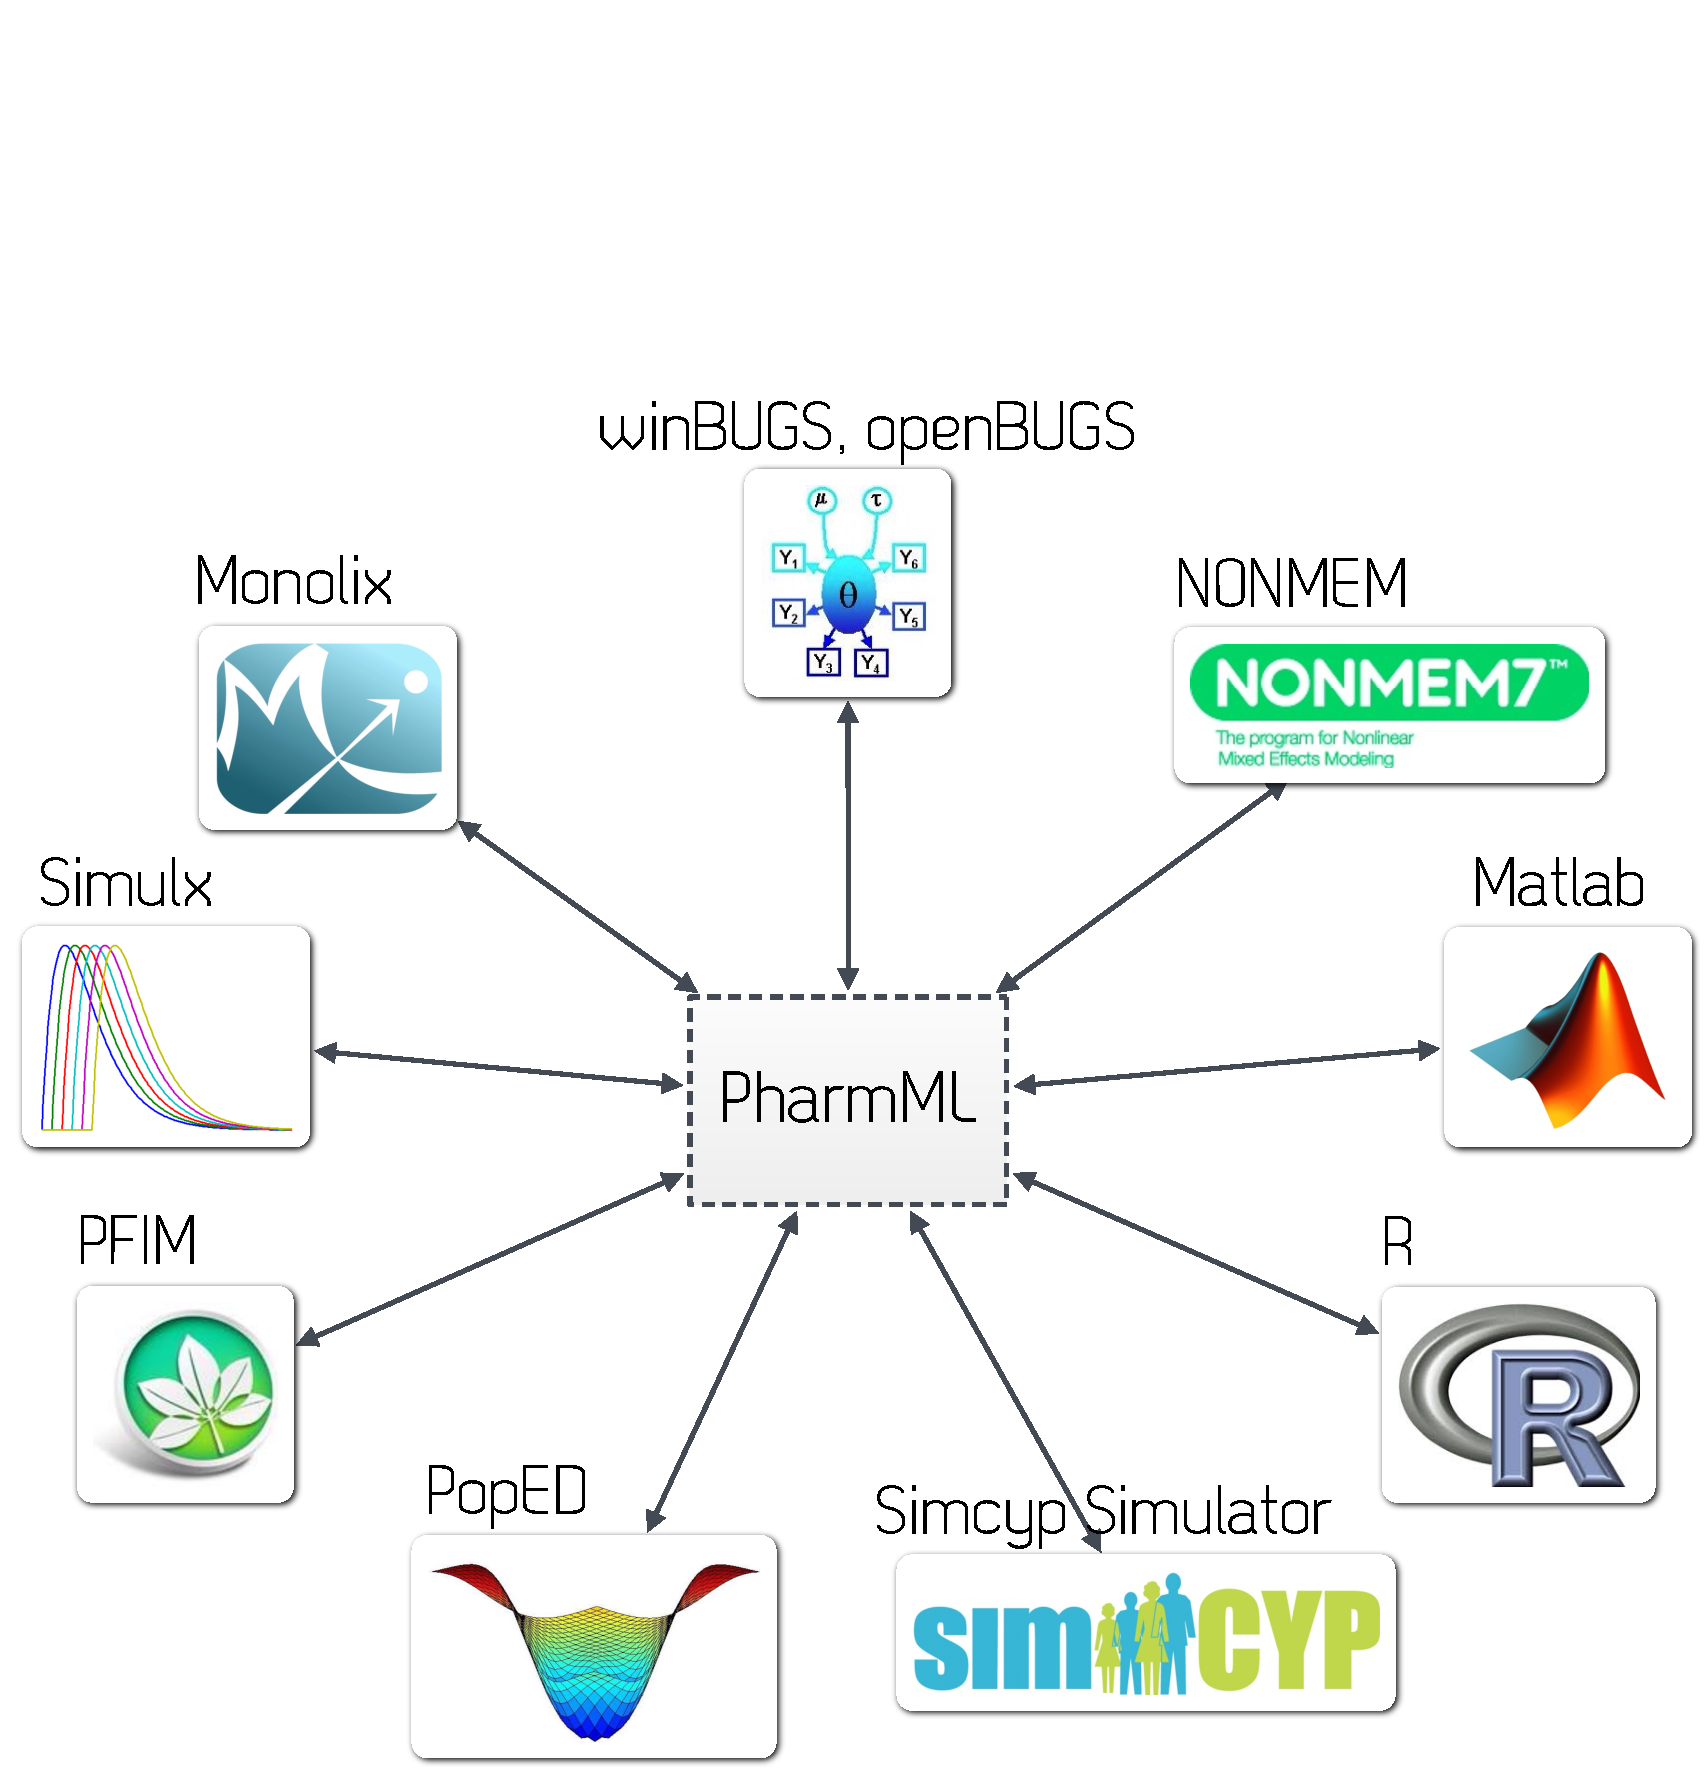
\includegraphics[width=0.60\linewidth]{pics/coverFigure}
 \label{fig:platformDDMoRe}
\end{figure}


\vfill

% Bottom of the page
{\large \today \\}
{1$^{st}$ public version, 0.2.1, was released on 21$^{st}$ November, 2013}

\end{center}
\end{titlepage} 


\cleardoublepage
\vspace*{\stretch{1}}
   \begin{minipage}{16cm}%
Copyright \copyright\xspace 2013-2015 The European Molecular Biology
Laboratory, Heidelberg, Germany\\* and Novo Nordisk A/S, Bagsv\ae rd, Denmark.
\end{minipage}


\cleardoublepage


\linenumbers
\tableofcontents


\newcommand{\matlab}{MATLAB\textsuperscript{\textregistered}}
\chapter{What is \pharmml?}
\label{chap:pharmml-what}

\section{The Problem}
%\begin{figure}[h]
%{
%\centring
\begin{wrapfigure}{r}{0.45\linewidth}
  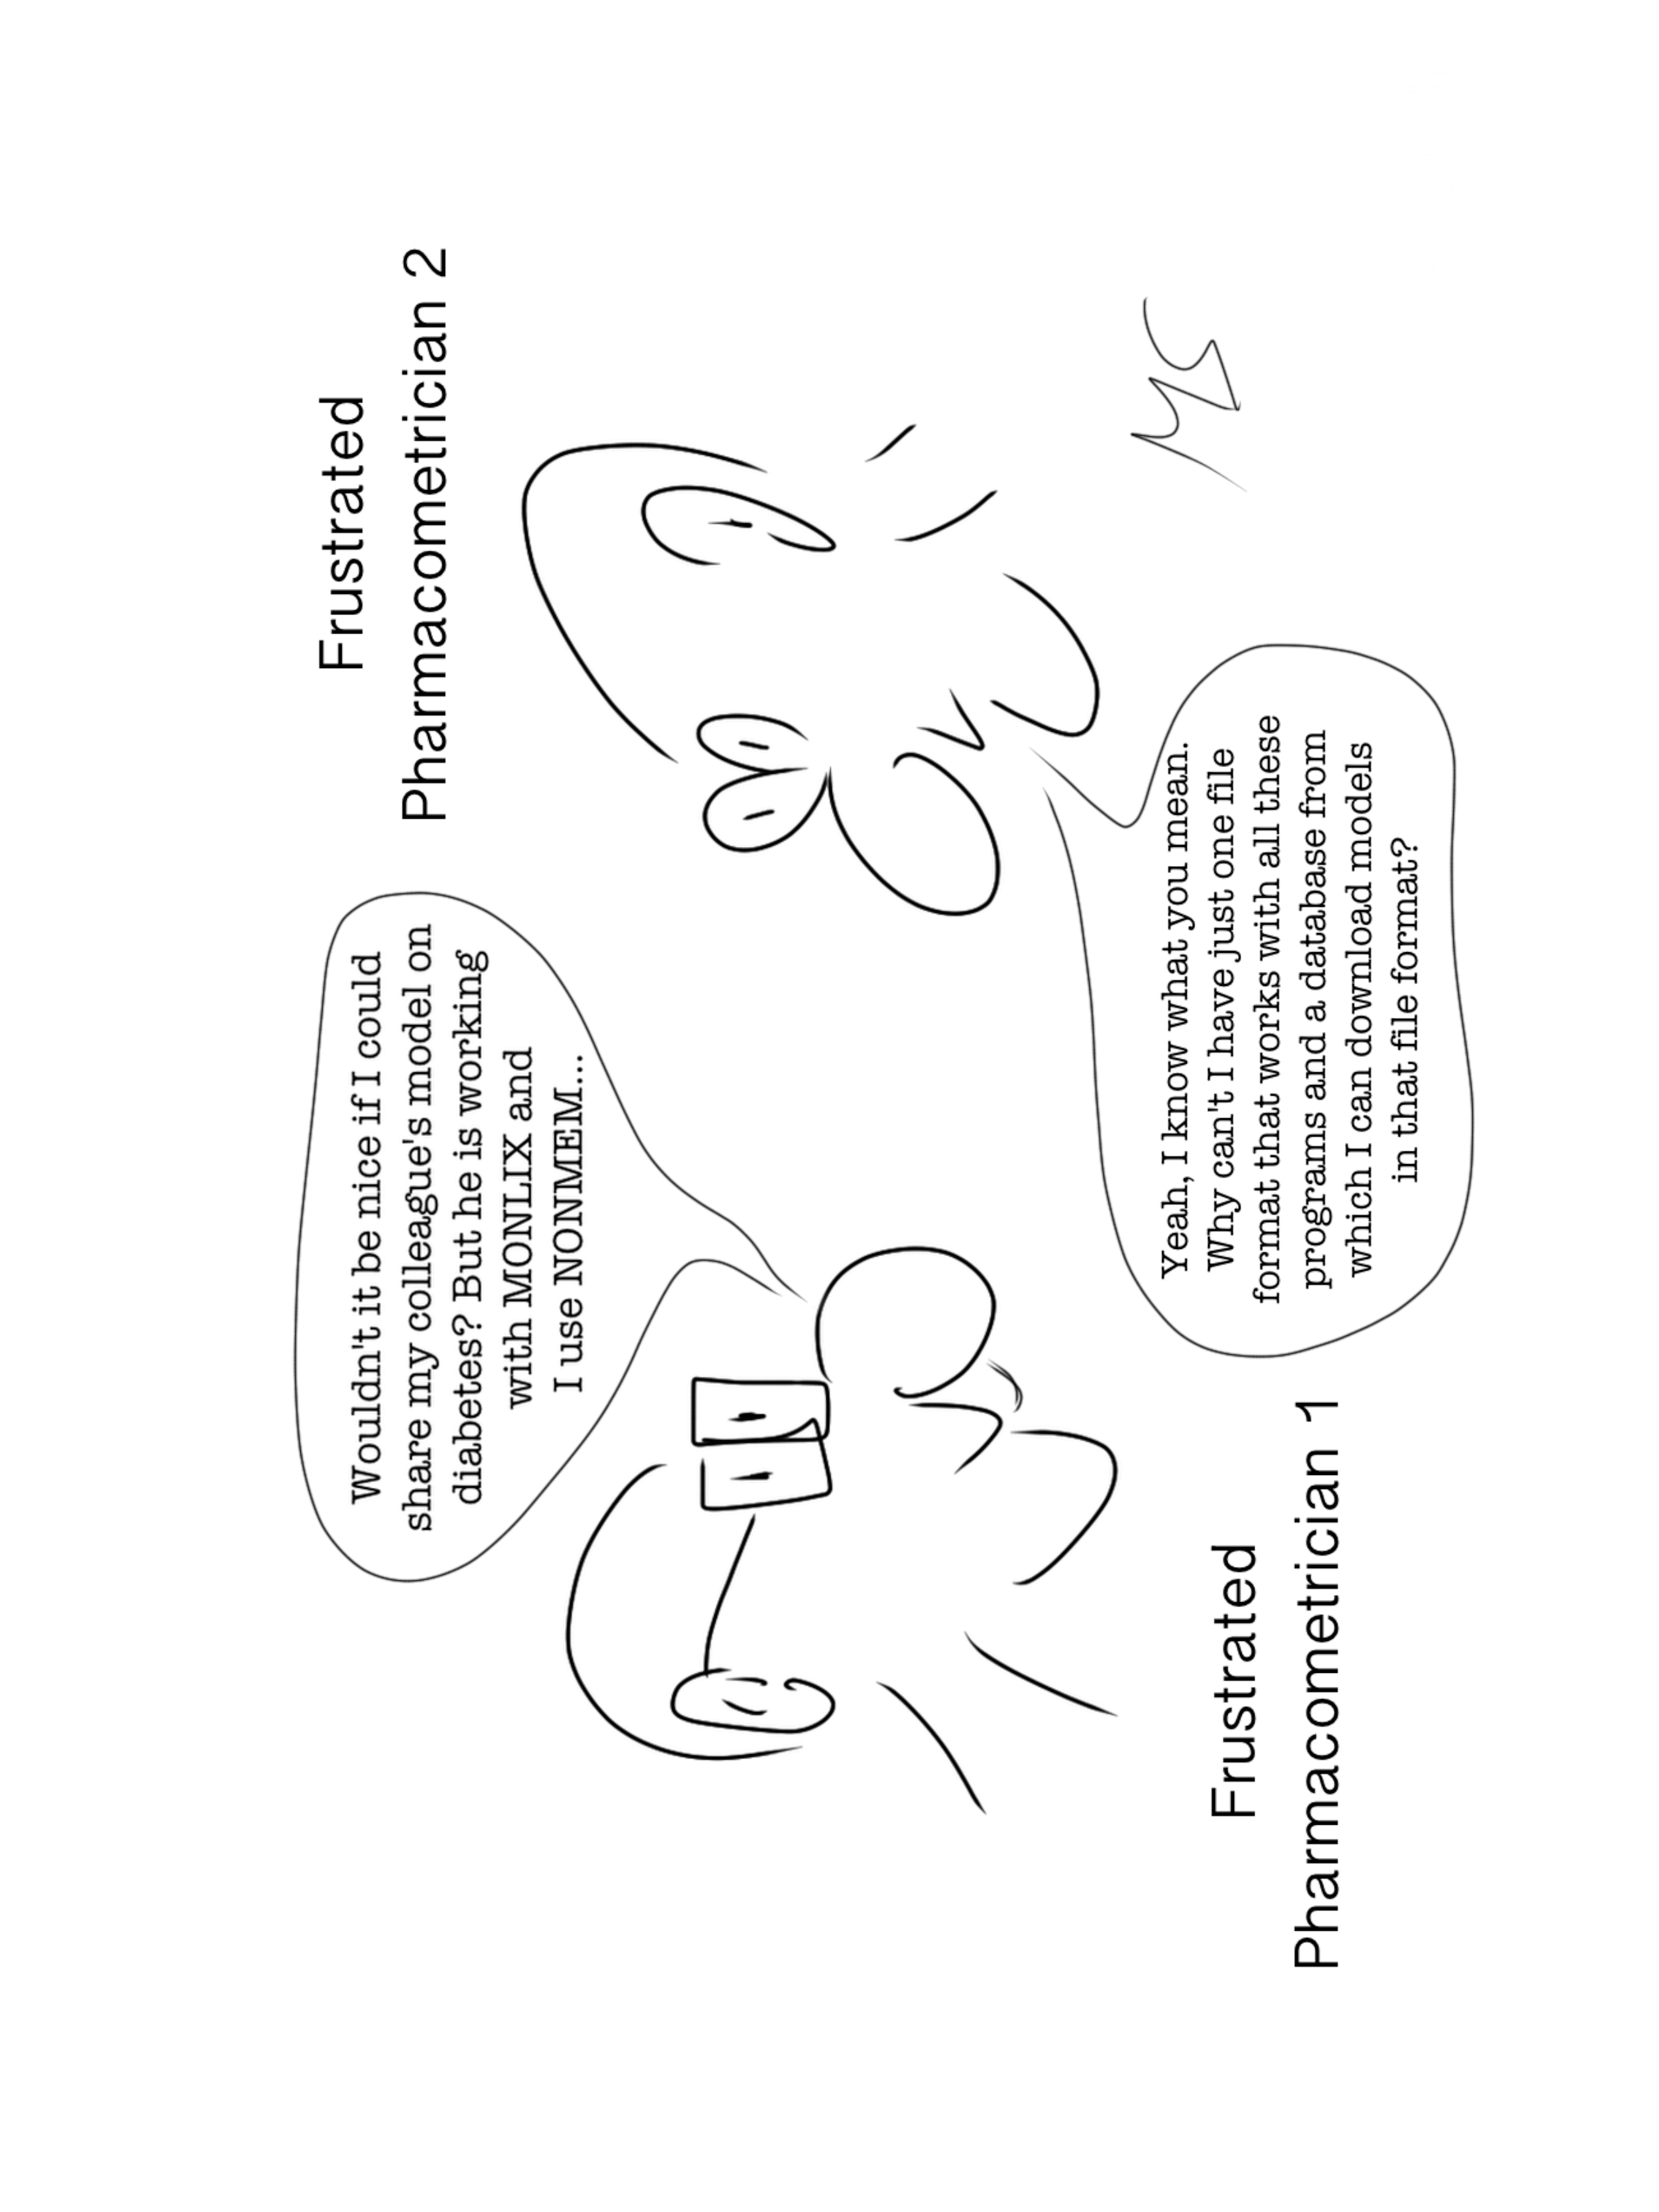
\includegraphics[angle=270,width=\linewidth,trim=90mm 80mm 80mm 50mm]{figures/MMLdudesFinal2}
\end{wrapfigure}
% }
%\end{figure}

%We could add to this cartoon, the caption: ``Someone, somewhere must be trying to solve this problem!''
%And if you read the \ddmore newsletter\footnote{Available from \url{www.ddmore.eu}.}, where this cartoon first featured, you will recall that our reply was, ``Well fortunately they are!'' We think this
The cartoon on the right summarises the principal problem that \pharmml addresses: namely,
the reliable exchange of pharmacometric models between software tools. What we are aiming
for is illustrated in Figure \ref{fig:platformDDMoRe}, where \pharmml is the exchange medium
for pharmacometric models for the main modelling and simulation tools in the field. This is
not an unreasonable goal and has been successfully realised in the field of Systems Biology.


 {\color{red} \scshape{SHOULD WE REWITE and REMOVE FIGURE?}}
 

In Systems Biology the problems our Frustrated Pharmacometricans complain of do not exist. Software
tools exchange models using the Systems Biology Markup Language (SBML; \url{www.sbml.org})
\cite{SBML} and many published models can be found in the BioModels Database
(\url{http://www.ebi.ac.uk/biomodels-main/}) \cite{BioModels2010}. Modellers don't worry about the
content of an SBML file; they rely on the fact that when they exchange it between their favourite
modelling tools, it just works. Crucial to its success has been an active community of tool
developers and modellers who have supported and used it during
that time. Equally important has been the provision of sophisticated software libraries (libSBML
and JSBML) that take away much of the pain a software tool developer would otherwise experience
supporting what is now quite a complex standard. It is a virtuous circle. Users demand their
modelling tools support SBML\@. Developers provide reliable SBML support using libSBML, which
enables them to give their users what they want. The more tools that support SBML, the more useful
it becomes. The cost of supporting SBML is not negligible but quality libraries like libSBML make
the cost acceptable.

\begin{figure}[htb]
\centering
  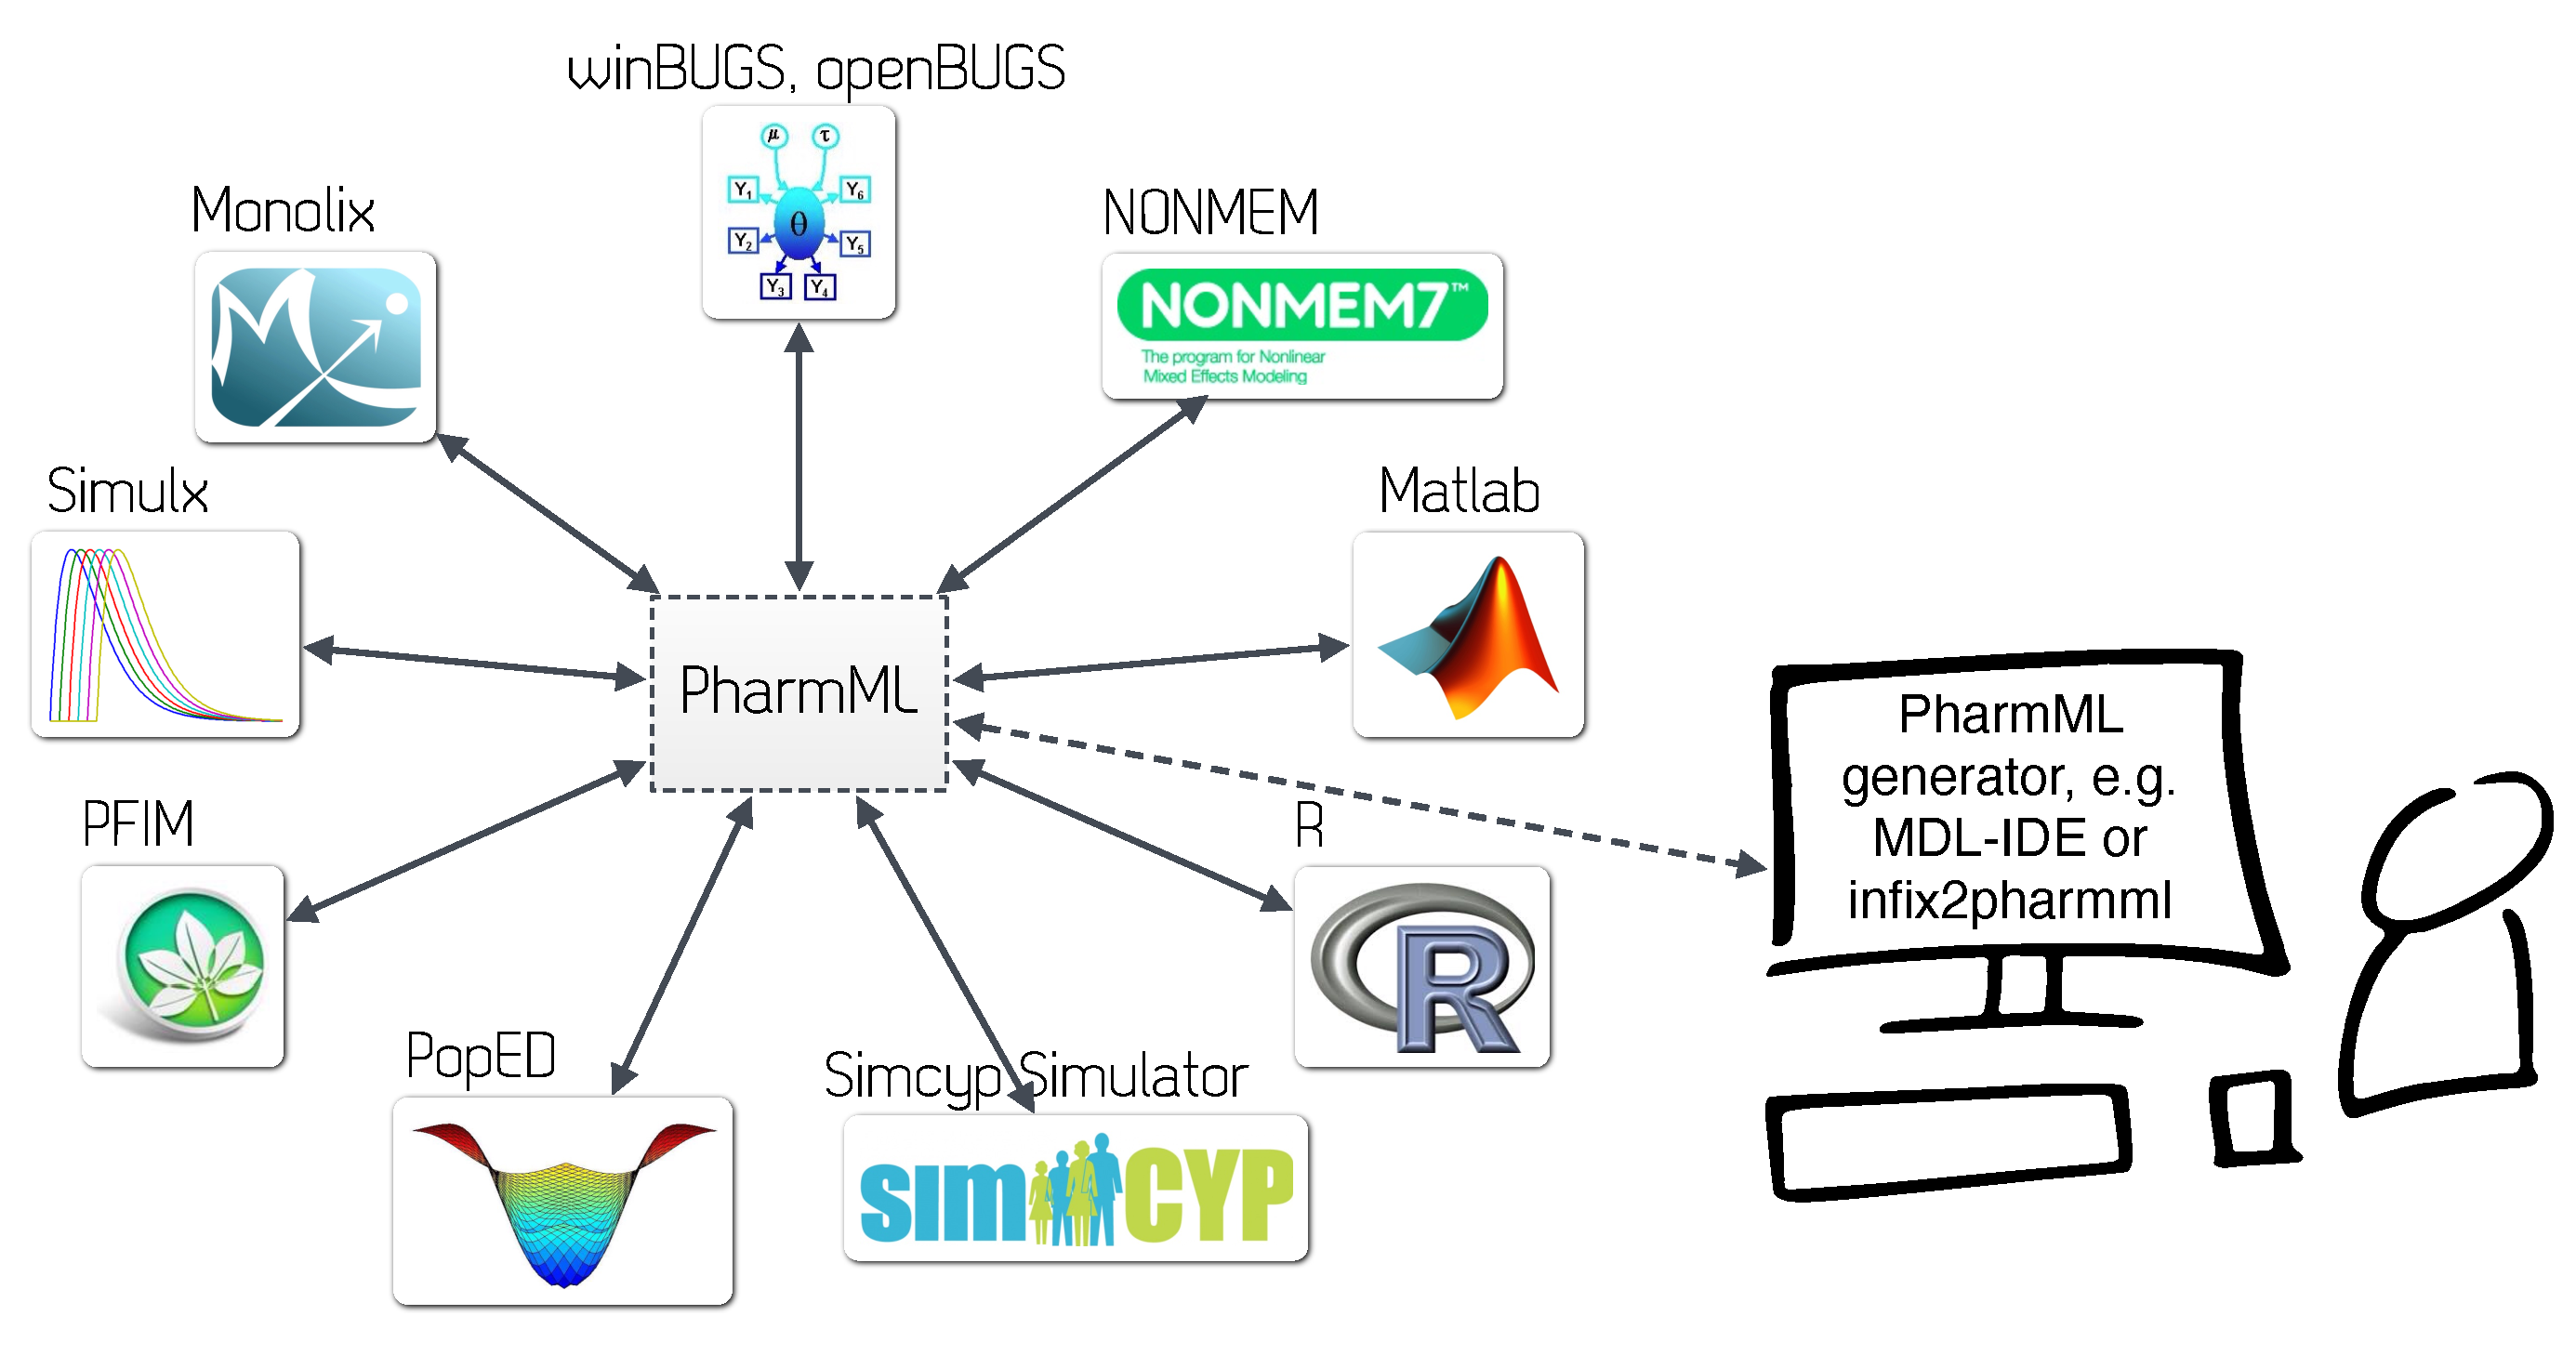
\includegraphics[width=0.95\linewidth]{pics/platformDDMoRe.pdf}
 \caption{Interoperability platform to exchange models via \pharmml.}
 \label{fig:platformDDMoRe}
\end{figure}

This lesson has not been ignored by the pharmacometrics community and in fact a number of years
ago the NLME consortium (a consortium of pharmaceutical companies now all part of \ddmore) started
to work on a very similar standard to \pharmml. This resulted in early drafts of an XML based exchange
language, called PharML, but work on it was unfortunately discontinued and the standard has never been
used and validated. There are a number of other exchange standards in related modelling fields, which we
have drawn on in the development of our work to varying degrees, including:

\begin{description}
\item[CellML] Supports the exchange and storage of computer based mathematical models of 
biological systems \cite{CELLML}.
\item[NeuroML] Supports the exchange and description of models ``to describe the biophysics, 
anatomy and network architecture of neuronal systems at multiple scales''\footnote{Quoted 
from \url{http://www.neuroml.org} on 15 Mar 2013.} \cite{NeuroML}.
\item[NineML] Describes neuronal networks in a ``simulator independent 
language''\footnote{Quoted from \url{http://software.incf.org/software/nineml} on 
15 Mar 2013.} that is design to interact with NeuroML \cite{ninemlspec}.
\item[SED-ML] Encodes simulation experiments of SBML and CellML models 
``to ensure exchangeability and reproducibility of simulation 
experiments''\footnote{Quoted from \url{http://sed-ml.org} on 15 Mar 2013.} \cite{sedmll1v1}.
\end{description}

So what is the solution to the problem? \pharmml. An XML based language that 
will be able to encode models from NONMEM, MONOLIX, BUGS and related tools. 
We intend this to be a community standard nucleated around the members of the 
\ddmore consortium. In addition we are developing a software library 
(libPharmML\footnote{\url{https://sourceforge.net/projects/libpharmml.ddmore.p}}) 
to help tool providers incorporate support of \pharmml and to facilitate its
general adoption in the field.

%%%%%%%%%%%%%%%%%%%%%%%%%%%%%%%%%%%%%%%%%%%%%%%%%%%%%%%%%%%%%%%%%%%%%%
\section{The Solution}
\label{intro:objectives}

Having described the problem, we here articulate the \emph{kind} of solution we wanted \pharmml to be.
Developing a language as complex as \pharmml is a difficult undertaking and we wanted to make sure
that we had some firm principles in place to help when designing the language. We've set these aims
and objectives below. \pharmml should:

\begin{description}
%\item[encode models used by pharmacometricians]
\item[describe the mathematics of a model] The language should not include 
information about the authorship of a model, its update history, or the nature 
of the disease process or drug that is being modelled. These aspects will be 
captured by the annotation of the \pharmml document and are out of scope 
of this specification.
\item[describe the task(s) associated with a model] The task(s), such as simulation 
or estimation, to be performed with a model should be encoded in the language.
\item[be declarative] The language should describe \emph{what} information is 
present in a model and \emph{what} the associated task(s) are. It should not 
describe \emph{how} the information is organised, or \emph{how} the task(s) 
should be performed.
\item[be platform independent] Language elements specific to a particular 
modelling tool should not be included. For example it should not describe 
a structural model using a name specific to PREDPP in NONMEM.
\item[serve as an exchange format for the \ddmore infrastructure] The language 
should either support features required by the infrastructure or provide extension 
mechanisms so that additional information can be associated with the \pharmml 
document.
\item[provide support for ontological annotation] The language should provide 
a mechanism for it to be annotated with information that is useful to describe 
the model, but which is beyond the scope of the \pharmml document itself.
\item[enable custom extension] Provide an extensibility mechanism so that 
software tools can associate additional, possibly tool specific information, 
with a \pharmml document.
\item[reuse existing standards where appropriate] Where an established 
information standard exists that can be used to represent information within 
the \pharmml document, we should adopt it.
\end{description}


%%%%%%%%%%%%%%%%%%%%%%%%%%%%%%%%%%%%%%%%%%%%%%%%%%%%%%%%%%%%%%%%%%%%%%
\section{PharmML \& SO -- workflow support and more}
\label{intro:workflows}
PharmML covers the input for a pharmacometric task, i.e. the model, trail design, 
according task description and experimental data. Another requirements 
posted for our work-package is to provide additionally a structure to store any type
of the numerical results coming from a target tool. This is now an ongoing 
effort and first draft specification of the so called Standardised Output (SO)
is already in use within the framework. 
\begin{figure}[ht!]
\centering
  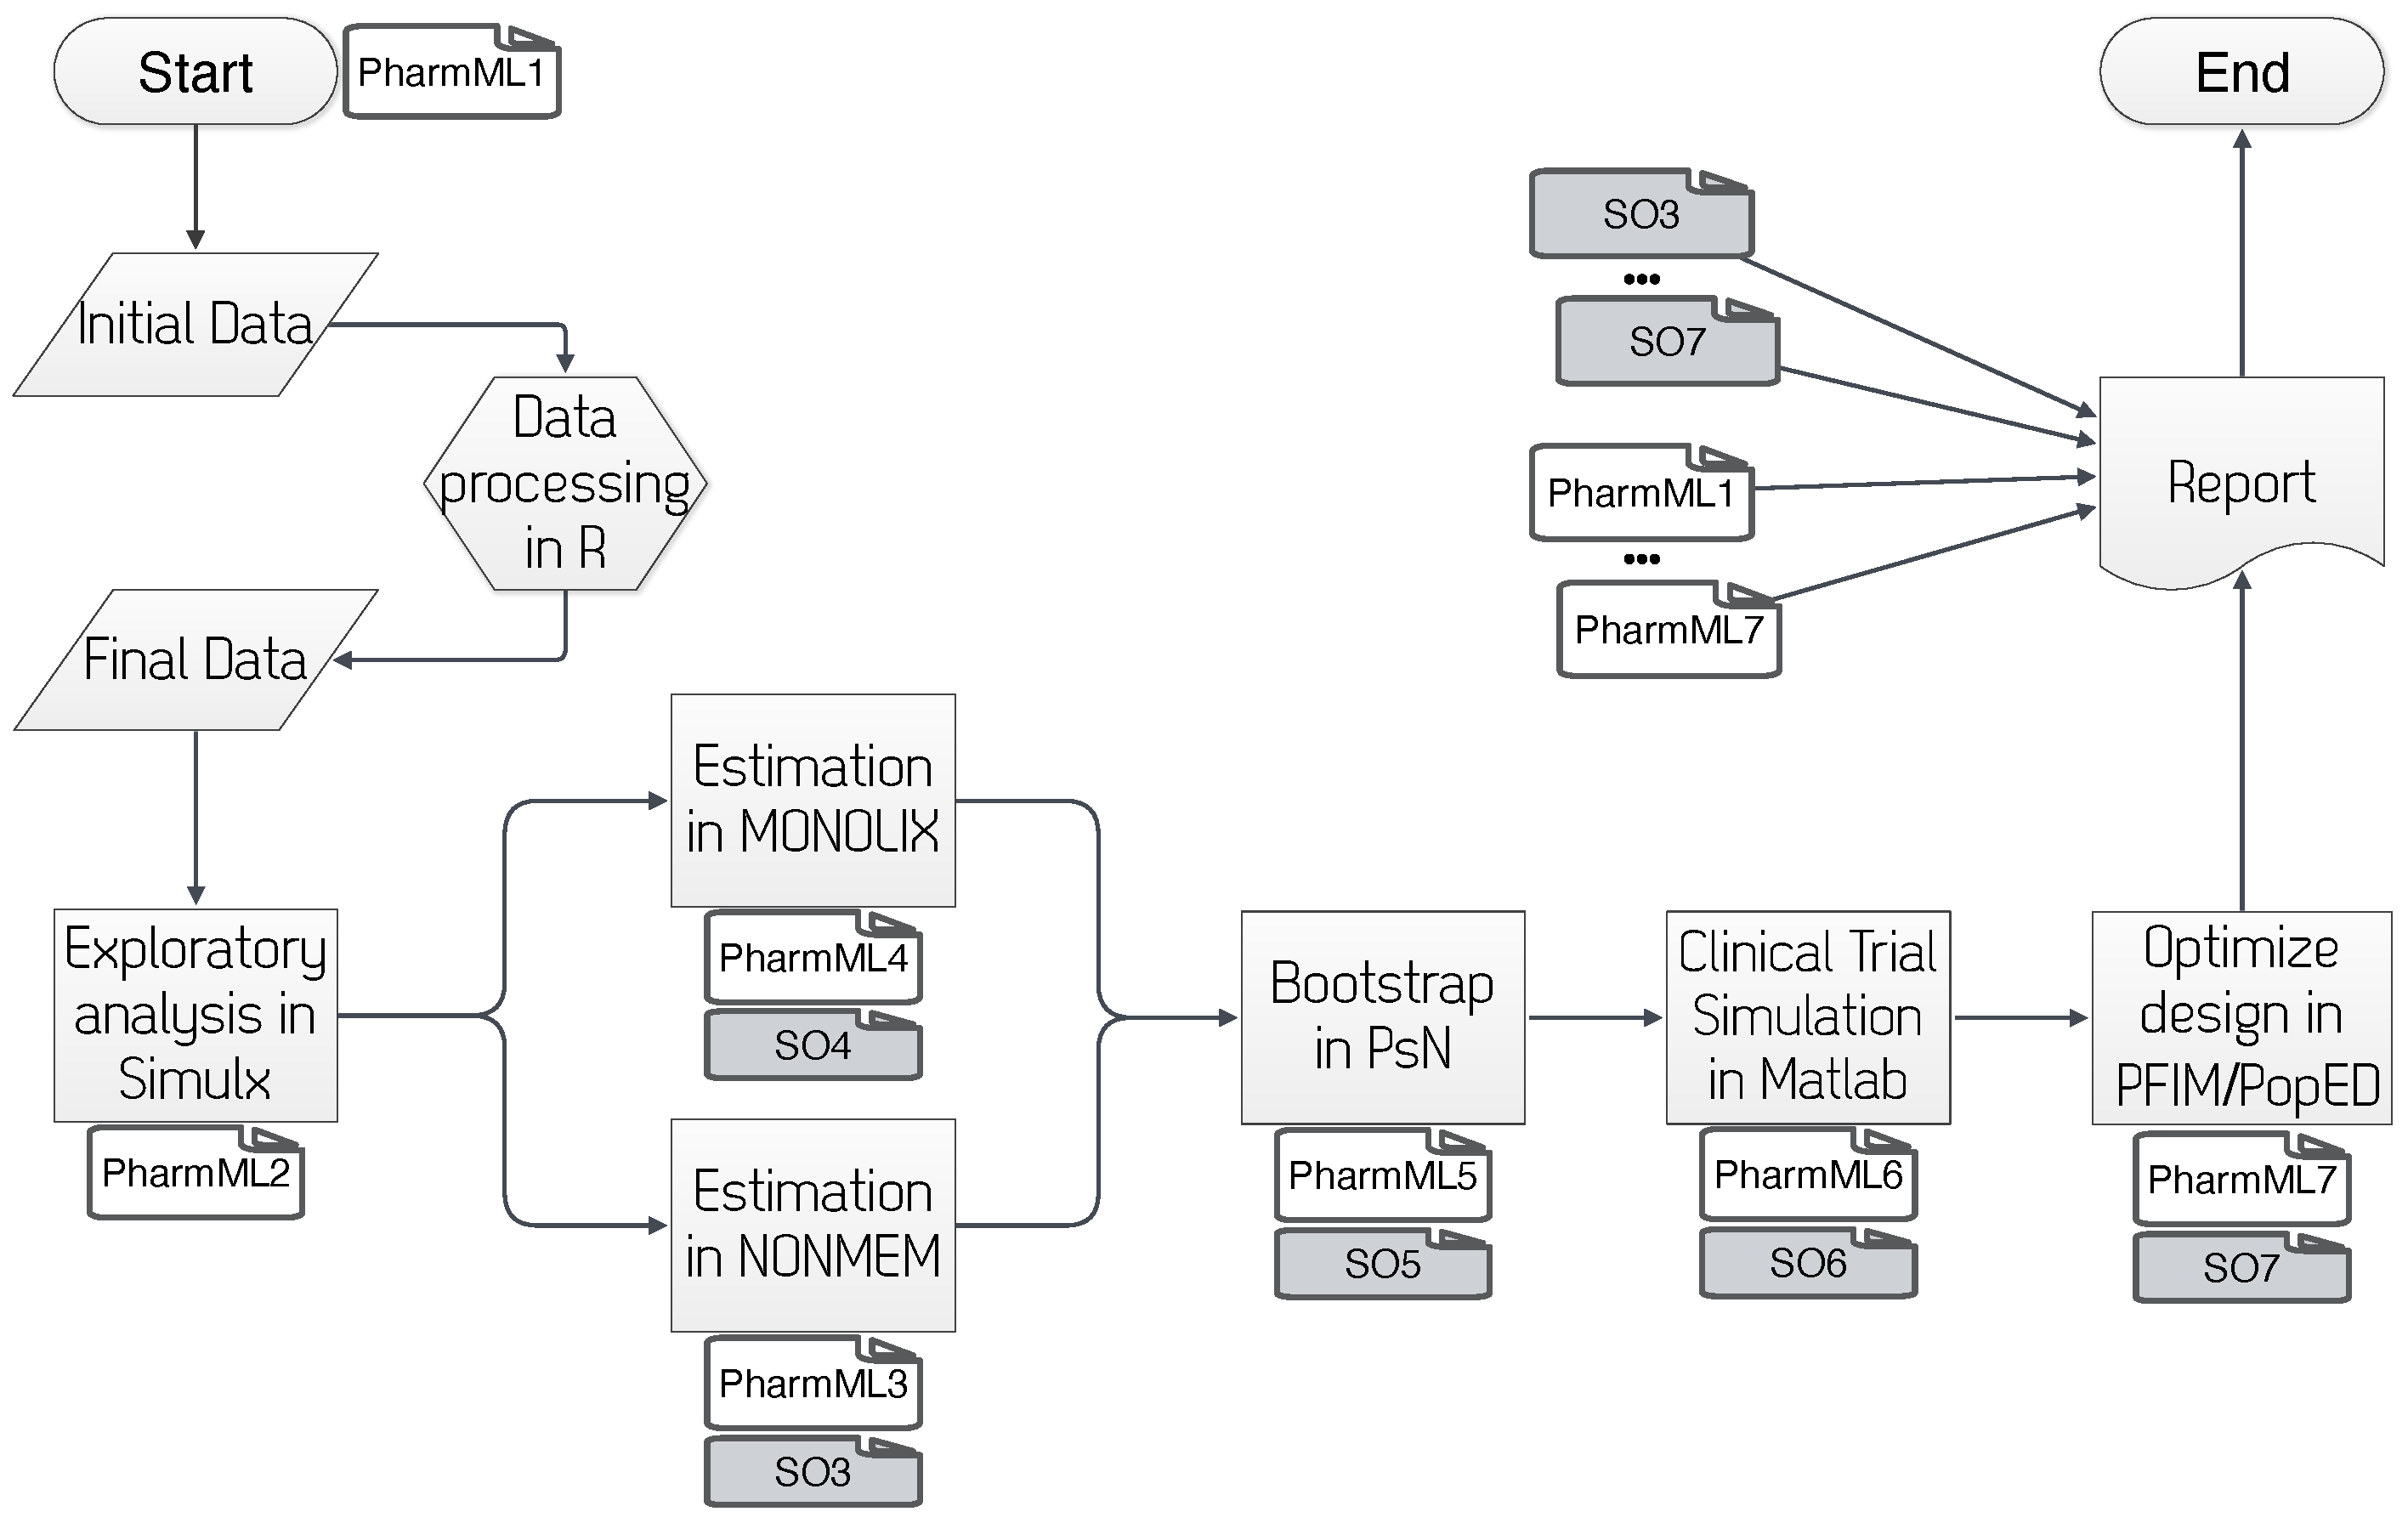
\includegraphics[width=0.95\linewidth]{pics/workflowPharmMLSO}
 \caption{PharmML and Standardised Output (SO) supporting a typical 
 workflow in Pharmacometrics featuring major target tools of the DDMoRe 
 platform. Here, it starts with data processing in R, which can consist of data 
 formatting, merging and/or missing-data imputation. After that an explanatory 
 analysis is carried out in Simulx, followed by estimation using either Monolix 
 or NONMEM. Subsequent steps are bootstrapping using PsN, clinical trial 
 simulation in Matlab and finally Optimal Design in either PFIM or PopED. 
 At every step of the workflow, the PharmML model can be stored and the 
 results following each step can be recorded in the corresponding SO file. 
 Documenting workflows in such a detailed way can potentially simplify 
 reporting and ensures reproducibility.}
 \label{fig:workflowPharmMLSO}
\end{figure}
A first public release of SO is planned in few months. Together, PharmML and SO 
are expected to facilitate:
\begin{itemize}
\item
Smooth and error-free transmission of models between tools
\item
Use of complex workflows via standardised model and output definitions, 
see for an example Figure \ref{fig:workflowPharmMLSO}
\item
Easier reporting and bug tracking
\item
Improved interaction with regulatory agencies regarding modelling and simulation
\item
Reuse of existing model resources, e.g. BioModels database
\item
Development of new tools and methods
\item
Expanding the community developing/applying pharmacometric models.
\end{itemize}


%%%%%%%%%%%%%%%%%%%%%%%%%%%%%%%%%%%%%%%%%%%%%%%%%%%%%%%%%%%%%%%%%%%%%%
\section{Creating PharmML coded models}
\label{intro:creatingPharmML}

As indicated in Figure \ref{fig:platformDDMoRe} once a model is encoded 
in PharmML it can be shared with any compatible target tool to perform simulation, 
estimation or optimal design. Modellers will be able in near future to write models 
using a human readable language also developed within DDMoRe, the 
Modelling Description Language, MDL (\url{http://ddmore.eu/mdl}). To facilitate its use, 
an Integrated Development Environment tool, MDL-IDE, is available, within which 
the model is automatically translated to PharmML and can be passed to PharmML 
compatible tools. Development of the MDL and the MDL-IDE is still on-going, 
but initial results are very promising. 

Alternatively, in cases when only the Structural Model is required, modellers can 
already use the web-editor infix2pharmml (\url{http://infix2pharmml.sourceforge.net}) 
to edit complete PharmML models. 


%%%%%%%%%%%%%%%%%%%%%%%%%%%%%%%%%%%%%%%%%%%%%%%%%%%%%%%%%%%%%%%%%%%%%%
\section{The \ddmore Consortium}

%Taken from the DDMoRe website need more work.

The Drug Disease Model Resources (DDMoRe) consortium aims to promote collaborative drug and disease
modelling and simulation research. Its aim is to develop tools and standards that will help the
consortium members and later the wider scientific community achieve this goal. Providing \pharmml
is a key goal of the consortium as it underpins a number of related deliverables of the consortium.
In particular:

\begin{itemize}
\item The \ddmore infrastructure in which \pharmml is used to exchange models between the different modelling tools.
\item The \ddmore model repository in which \pharmml will be used to upload and export models to and from the repository. It will also serve as the storage medium for the repository.
\item The \ddmore library of reference models and data-sets, which will provide models in several therapeutic areas. These models will be encoded using \pharmml.
\end{itemize}

The contribution of the \ddmore consortium members in guiding and reviewing the standard has been enormous.
As the standard evolves their role in using and then promoting the standard to the wider community will be invaluable.

Peer review is important in the development of \pharmml and to date we have hosted number of
face-to-face meetings since the development of \pharmml commenced in August 2011. These meetings were:

\begin{itemize}
\item A number of \ddmore consortium meetings in Leiden and Hoofddrop, in the years 2012--2014.
\item The \ddmore technical workshop hosted by Novo Nordisk in Copenhagen, 28--30 Jan 2013.
\item Two \pml technical workshops hosted by University of Pavia, November 2013 \& 2014 .
\end{itemize}

\section{How \pharmml was developed}

\pharmml was designed and implemented by a relative small group of individuals, 
but its development has very much been a collaborative process. At the beginning of 
this project we had a number of development guidelines that we adhered to. We aimed to:

%\begin{figure}[ht!]
%\centering
%  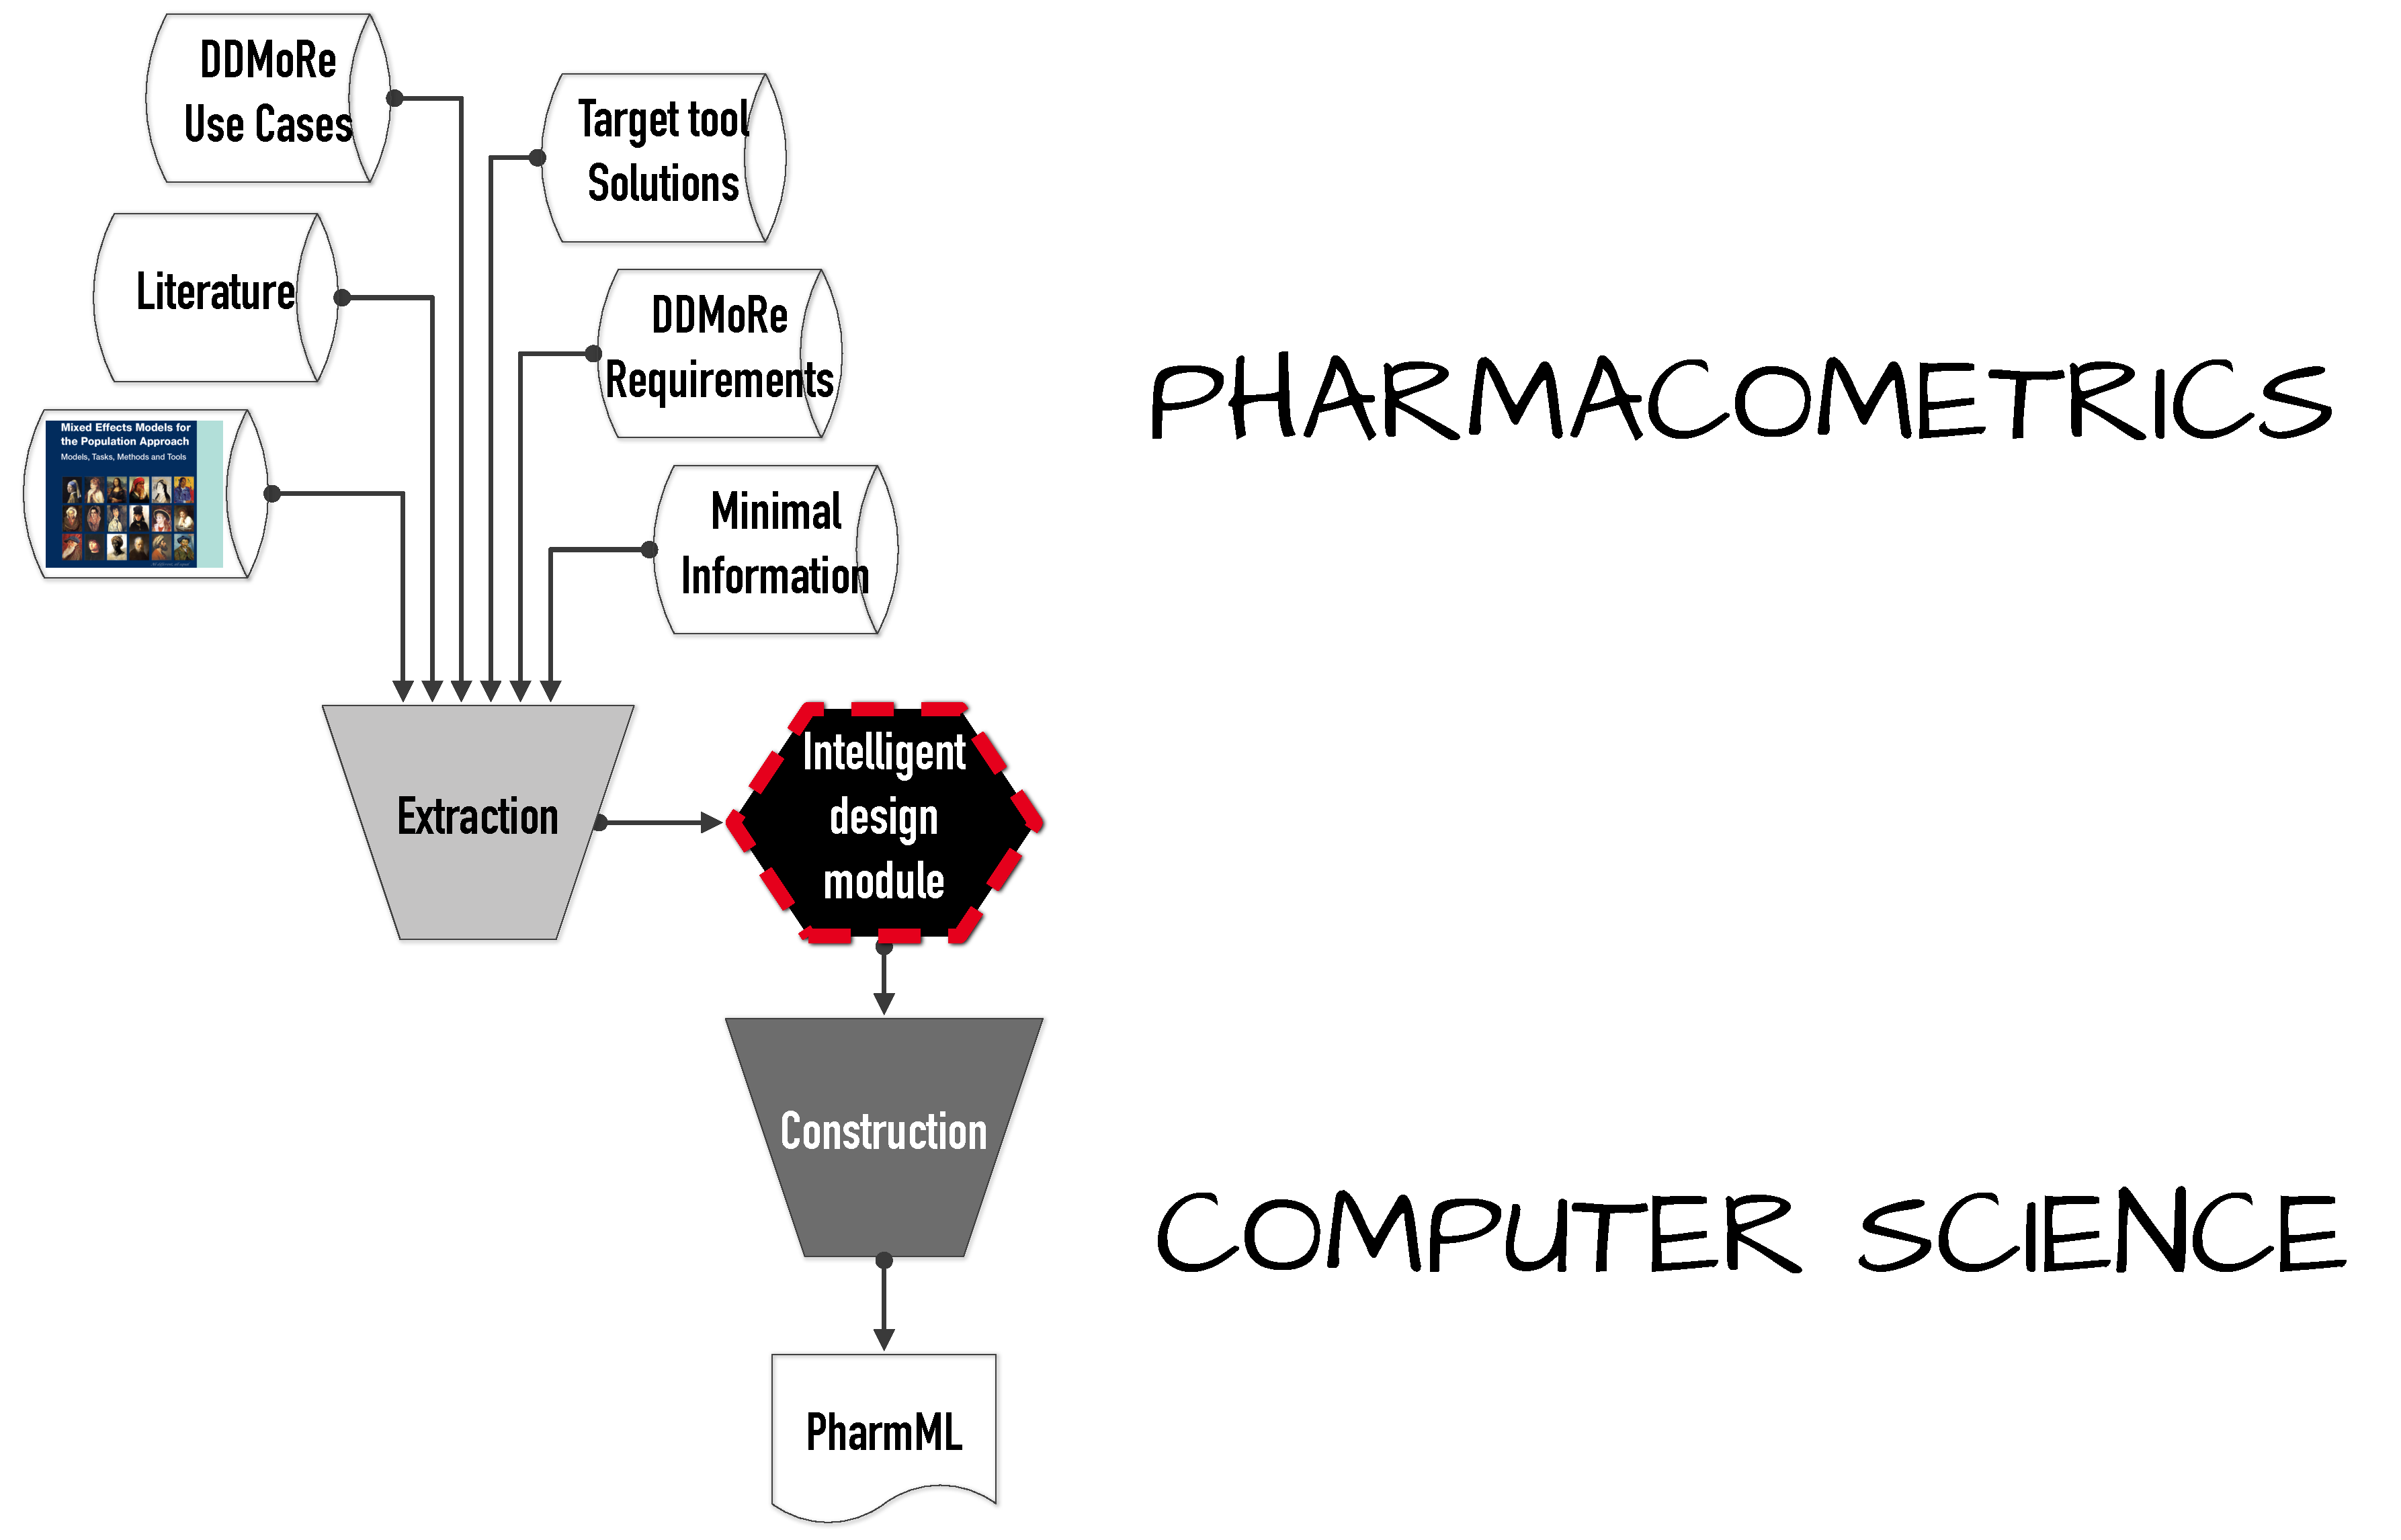
\includegraphics[width=0.9\linewidth]{pics/pharmmlDevelopment}
% \caption{PharmML development process}
% \label{fig:PharmMLdevelopment}
%\end{figure}

\begin{itemize}
\item start with a limited scope and expand the functionality we encode over time.
\item drive development using use cases which reflect the current scope.
\item test the implemented use cases by generating executable models.
\item have frequent review meetings with experts to make sure we are on the right track.
\item use existing technology standards if it is possible and reasonable to do so.
\item use existing information standards if applicable to avoid re-inventing the wheel.
\item make sure the standard is in a form and uses names and terms that make sense to the expert community.
\end{itemize}

In the first half of 2014 an Interoperability Group within the DDMoRe consortium 
was appointed to facilitate the testing of \pml and the interoperability platform driven 
by it. This typically includes 
\begin{itemize}
\item
Creating a MDL coded model in the MDL-IDE (see Figures \ref{fig:platformDDMoRe} 
and \ref{fig:workflowPharmMLSO} for an schematic representation of this and 
the following steps).
\item
Translation from MDL to PharmML.
\item
Translation from PharmML to a target tool language, e.g. MLXTRAN coded model 
for use in Monolix/Simulx or NMTRAN for NONMEM.
\item
Performing a task in a target tool and the export of results into SO.
\end{itemize}
Initial results are very promising, with a number of models being successfully processed 
though this pipeline providing a proof-of-concept for the interoperability concept. 
Figure \ref{fig:DDMoReTimeline} gives an overview of the development timeline, 
more details can be find in the detailed changelog in chapter \ref{cht:changeLog}.

\begin{figure}[ht!]
\centering
  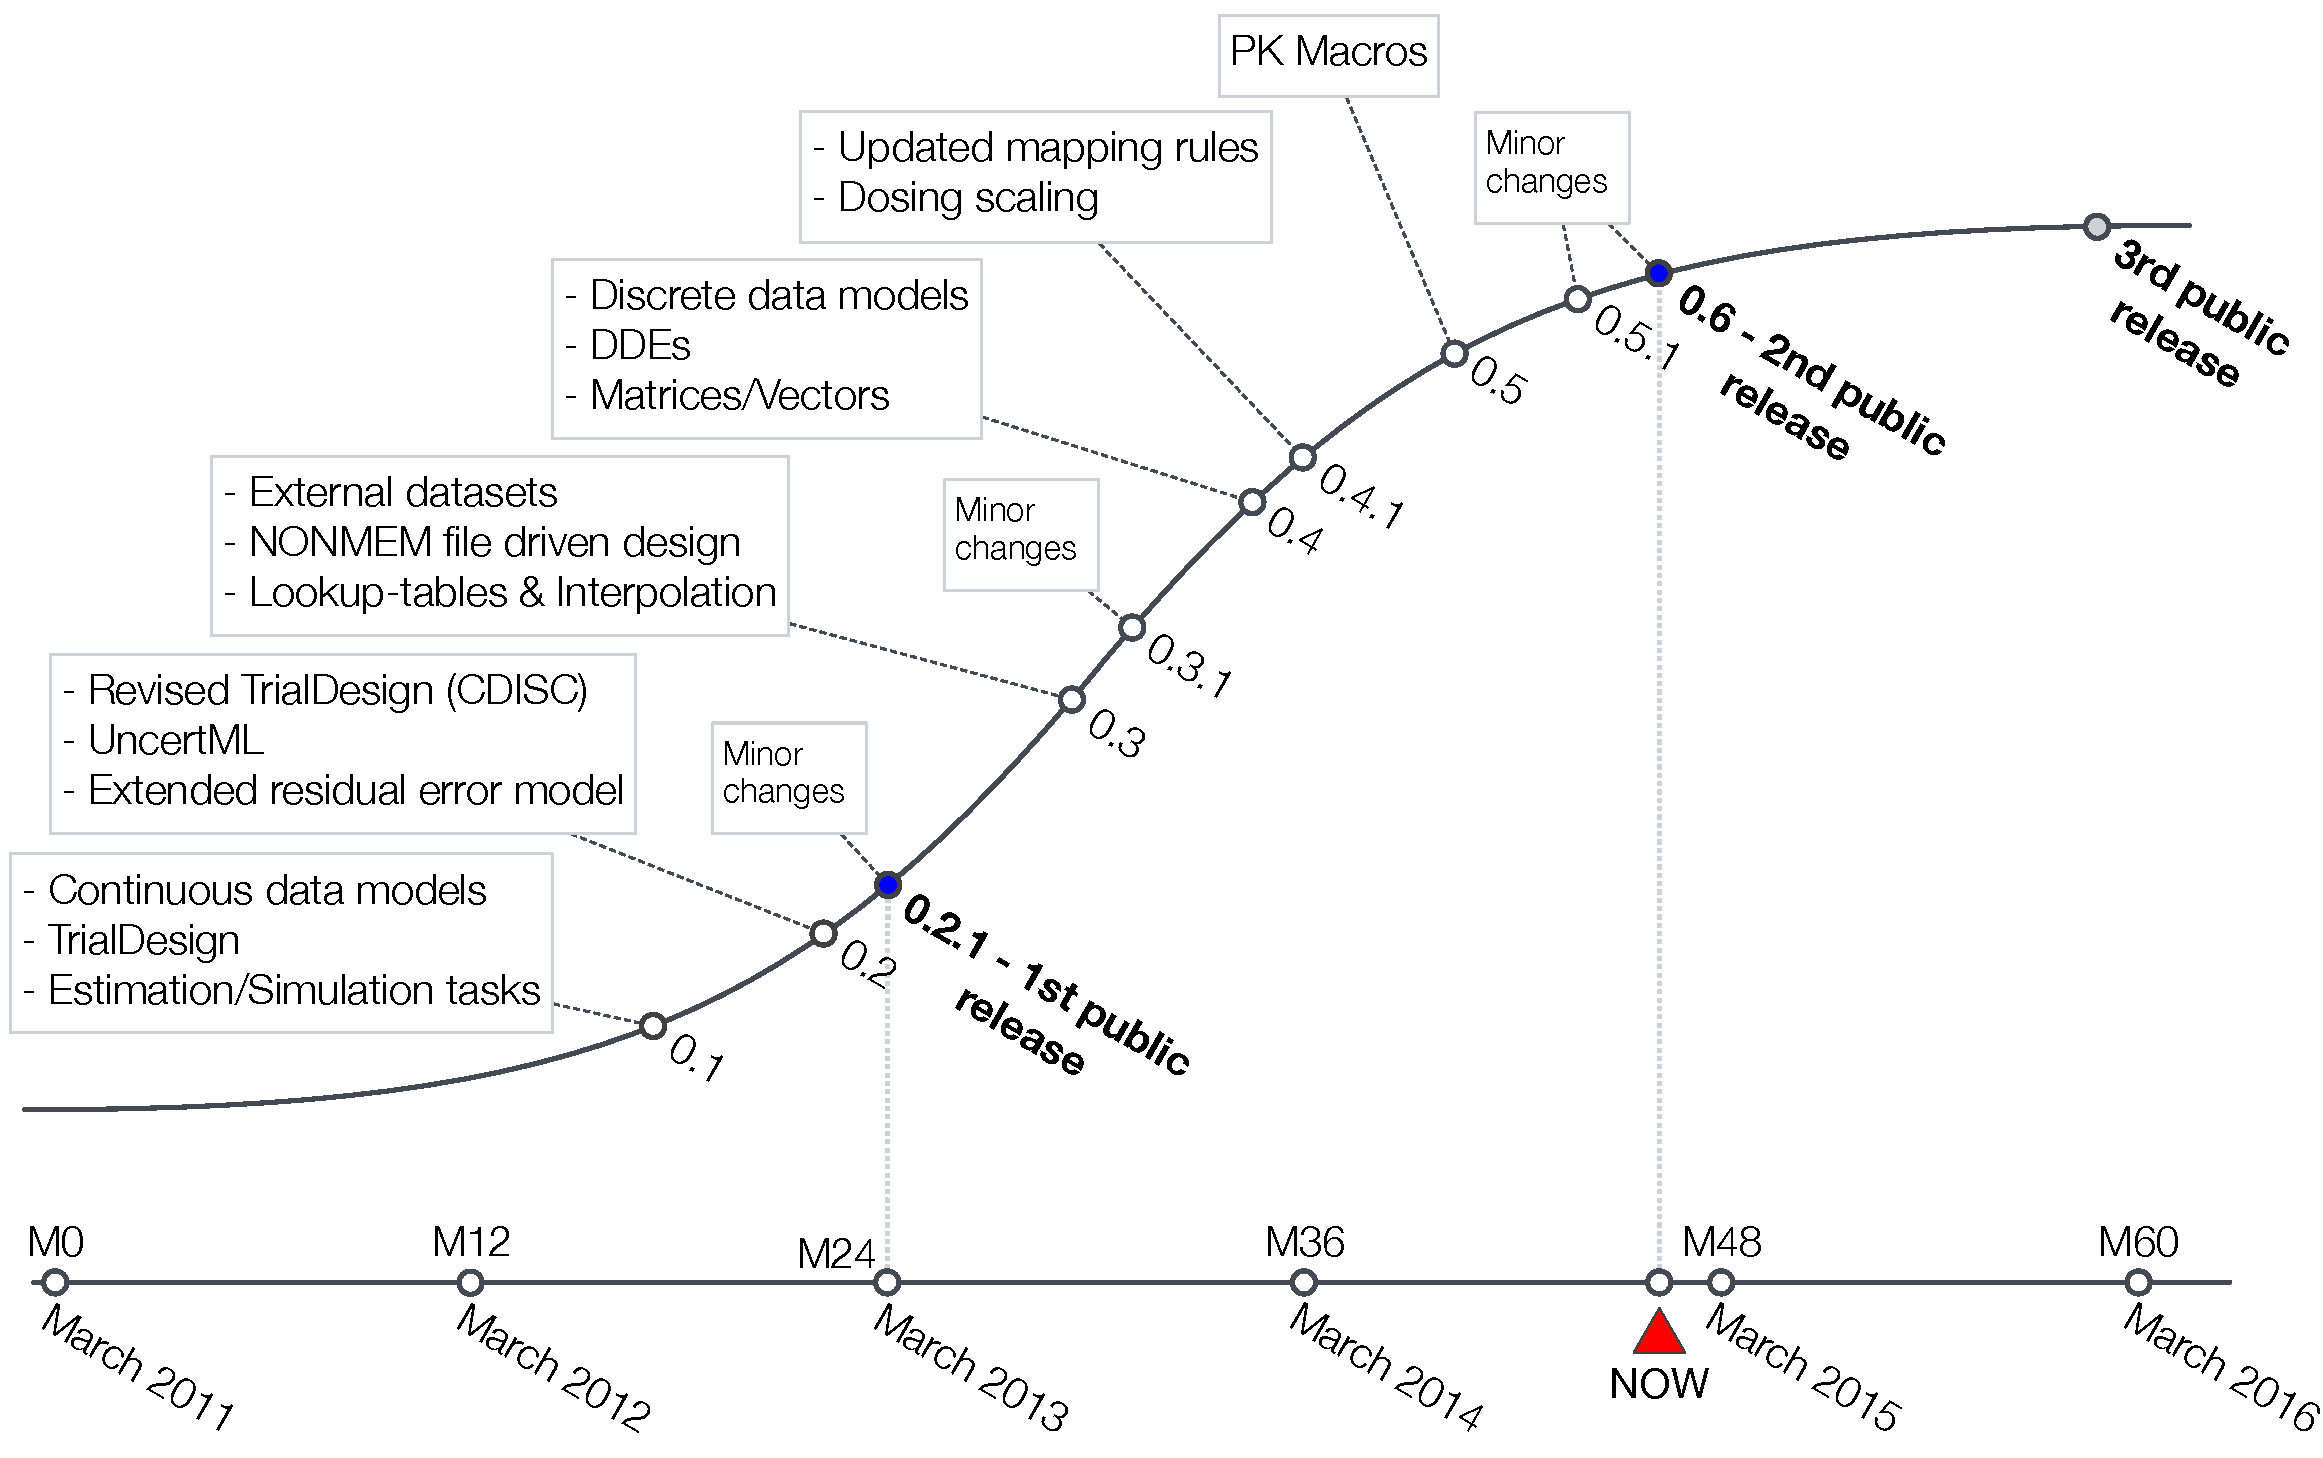
\includegraphics[width=0.95\linewidth]{pics/Timeline.pdf}
 \caption{Timeline of the \pharmml development process, deliverable schedule and version 
 features.}
 \label{fig:DDMoReTimeline}
\end{figure}

\section{Imperative or Declarative?}

In developing \pharmml we have designed it to be a declarative language (see section \ref{intro:objectives}).
While we feel this is the best approach to take for an information exchange langage, it does present us
with number of challenges when dealing with NONMEM, the leading tool in the field. Despite
having a specifically defined language (NM-TRAN \cite{NONMEM:2009}), NONMEM offers a lot of flexibility
to the user, and experienced users can make NONMEM do things that it was never designed to do, to a large
extent because the imperative approach used in NONMEM facilitates this.

The challenge is to convert from the imperative to the declarative language, because there are 
many ways to do the same thing in the imperative language. Therefore, generating 
a \pharmml document from a NONMEM control stream is challenging.

 % It is not the purpose of this document to conduct a detailed comparison between these two approaches but it is important to keep the characteristic differences in mind. One of the main objectives of the DDMoRe project and specifically work-package 4 (WP4) is the building a bridging technology for alternative approaches within one framework. PharmML, the XML based exchange standard which is now available in this first specification is the core element of this interoperability framework.

 % Nevertheless, the differences between these softwares, which manifest themselves mainly in the \emph{imperative} approach of NONMEM versus the \emph{declarative} approach of Monolix, created a chance to a cover broad spectrum of methods and ideas developed over decades. On the one hand FORTRAN-based NONMEM, despite having a specifically defined language (NM-TRAN \cite{NONMEM:2009}), offers almost
 % unlimited flexibility to the user. It can be viewed as a general purpose computational platform and in fact it has been developed
 % as such and can be compared to Matlab or Mathematica (REFs). On the other hand Monolix has been specifically developed for use in pharmacometrics. Although being very flexible, it is based on MLXTRAN, a constantly developing declarative language, defining very precisely the types of allowed models and algorithms.

%Let's put the NONMEM Monolix discussion here and then say that we have adopted a declaritive approach and say why it is better. Need to be careful 
%here to make sure we don't imply that in consequence Monolix is better than NONMEM.

\section{The Evolution of PharmML}
	
This document represents the second public release of \pharmml. The first one was released  
on 21$^{st}$ November, 2013, \cite{Pharmml_021}.

Any piece of software is upgraded as users request new features and developers find better 
ways to do the same thing. A successful standard is no different and with success in mind we 
expect \pharmml to evolve and change further as it is subject to the same influences. To manage this 
process we have adopted the following strategy to record versions of the \pharmml specification.

\paragraph{Version number}
\label{intro:versioning}

To record changes in the specification we will use the following three level numbering system, of the form
$x.y.z$. The levels correspond to the following types of revision:

\begin{description}
\item[$x$ major] Significant new features or radical change of design.
\item[$y$ minor] New features or evolutionary design changes.
\item[$z$ patch] Error corrections.
\end{description}


%%%%%%%%%%%%%%%%%%%%%%%%%%%%%%%%%%%%%%%%%%%%%%%%%%%%%%%%%%%%%%%%%%%%%%
\section{Feedback}

User and developer feedback is important. Typically,
this feedback will be in the form of a specific issue: either to report defects identified in
the specification or to request new features. Either way the specific issues can be submitted
to the tracker at: \url{https://github.com/pharmml/pharmml-spec/issues}. In some cases it is practical to raise
an issue that is broader than a specific issue or requires some discussion within the community. 
Here the contact is the \pharmml forum at \url{http://pharmml.org}.



\chapter{Scope of \pharmml}\index{PharmML!scope} 
\label{chap:scope}


\section{Introduction}

The scope of pharmacometric models is very wide, as such models can be empirical as well as
mechanistic; describe continuous as well as discrete data types; and be deterministic, stochastic
or a mixture of both. It is a challenging endeavour to accommodate this variety of possibilities
under one computational standard, therefore it is indispensable to split the task into multiple
steps of subsequent specifications and to define precisely the scope of every release.

In this chapter we define the scope of the functionality in
\pharmml, i.e. what information a \pharmml document can
represent. As is common practise in software engineering we have 
described the functionality as a set of ``features''.  It is important to remember 
that this specification is the second public release of \pharmml and over remaining 
time we expect additional features to be provided by future releases of the language.

The language is organised into three sections, which we believe naturally
describe the logical organisation of a pharmacometric model and its
associated tasks. Consequently we have grouped the features to match this
organisation. The sections are:
\begin{description}
\item[Model Definition] A description of the model, incl.\ the structural model, the model
  parameters, relevant covariates, the variability components, and the observations.
\item[Trial Design] A description of the design of a clinical trial associated with the model
  (for example a trial from which data is available to estimate the parameters of the model or
  a trial to be simulated with the model).
\item[Modelling Steps] A description of steps or tasks performed with
  the model. Typically this describes how the model has been used, for
  example to estimate its parameters or to perform a simulation.
\end{description}

\section{Model Definition}
\subsection{Structural Model}

\pharmml can encode:
\begin{itemize}
\item{A structural model defined by a set of algebraic equations.} Typically the explicit solution to a simple PK model, or a dose-response model.
\item{A structural model defined by a system of ODEs with initial conditions.} 
%\item{A structural model defined in \sbml format.}
\item{Delay Differential Equations (DDEs).}
\item{Compartmental PK models implemented using PK macros.}
\end{itemize}

\subsection{Covariate Model}

\pharmml can encode:
\begin{itemize}
\item{Continuous covariates.} These can be sampled from a probability distribution, 
used with an applied transformation and interpolated.
\item{Categorical covariates.} These can also be sampled from a probability distribution.
\end{itemize}

\subsection{Parameter Model}

\pharmml can encode:
\begin{itemize}
\item{Gaussian models with linear or non-linear covariate model.}
\item{General, equation based model such as those described in \cite{Keizer:2011aa}.}
\item{Random effects at arbitrary levels of variability.}
\item{Correlation of the random effects, described by a correlation or covariance matrix.}
\end{itemize}

\subsection{Variability Model}

\pharmml supports the following levels of variability:
\begin{itemize}
\item{Between-Subject Variability (BSV).} Aka inter-individual variability (IIV).
\item{Inter-Occasion Variability (IOV).} Such as within-subject variability.
\item{Higher levels of variability above BSV.} Such as variability between countries or centres.
\item{Lower levels of variability below IOV.} Such as variability between sub-occasions within occasions.
\end{itemize}

\subsection{Observations Model}

\pharmml supports the following observation model:
\begin{itemize}
\item{Continuous data models.} A residual error model applied to one or more observation variables..
%\item{Autocorrelation of the residual errors in a continuous observation model.}
\item{Discrete data models such as}
\begin{itemize}
\item{Count data models.} Such as Poisson, negative binomial, zero-inflated Poisson models etc.
\item{Nominal and ordered categorical models.} Logistic regression, proportional odds models etc.
\item{Time-to-event models.}
\end{itemize}
\end{itemize}

\section{Trial Design}

\subsection{Dataset based}

\pharmml supports external NONMEM/Monolix datasets which can be sourced 
to provide the full study design and the according experimental records. 
 
\subsection{\xelem{TrialDesign} based}

\pharmml can encode the following features of a trial design \emph{explicitly}:
\begin{itemize}
\item{Bolus and infusion dosing.}
\item{Multiple dosing regimens including mixed bolus and infusion.}
\item{Single, Repeated and Steady state dosing.}
\item{Dosing to more than one compartment.}
\item{Simple, parallel and cross-over designs.}
\item{Washout periods.}
\item{Occasions -- defined by time interval within a treatment epoch.}
\item{Trials with different centres or other levels of organisation above study arms}
\end{itemize}

\section{Modelling Steps}

\pharmml can encode the following features related to the task(s) associated with a model:
\begin{itemize}
\item{Estimation utilising the maximum likelihood principle.}
\item{Simulation of the model.}
\end{itemize}

\section{General}

\begin{description}
\item{Metadata annotation} Provides support to enable metadata
descriptions of the \pharmml document.
\item{Extension mechanism} Provides support to enable the extension of
the \pharmml document.
\end{description}



\chapter{Mathematical Representation}
\label{chap:mathsdefn}


\section{Introduction}
This chapter deals with the mathematical description of models which can be 
encoded in PharmML. The figure \ref{fig:indivModel} visualises the task every 
modeller is faced with -- find a model (solid line) which explains the experimental 
data (diamonds). A perfect mathematical model, given error free experimental 
measurements, would explain the underlying mechanism and therefore fit every 
measurement. The complexity of the human body makes detailed mechanistic 
representation impossible, so the models we use are only approximations of a 
physiological system under consideration with multiple sources of uncertainty 
we have to account for, see Figure \ref{fig:basicEquation}.

%{\Large
%\begin{eqnarray}
%&& Experimental \;data = Model \;Prediction + Error \nonumber
%\end{eqnarray}
%}
\begin{figure}[htbp]
\centering
 
\includegraphics[height=12mm]{pics/ModelEquation.pdf}
\caption{A basic equation visualising the relationship between experimental 
data and model prediction.}
%\caption{Basic mathematical model for frequently sampled individual data. 
%The black diamonds stand for experimental data, the solid line for the time 
%course of concentration as predicted by a mathematical model.}
\label{fig:basicEquation}
\end{figure}

Additional aspect is the difference between individual and population approach. 
In the former case, usually when dealing with animal or preclinical studies, 
frequently sampled data is available and one can estimate individual's PK and 
PD parameters, see Figure \ref{fig:indivModel}. In clinical practice however, 
the situation is quite different, Figure \ref{fig:popModel}. More data records 
in total are available but it's often impossible to estimate subject specific 
parameters. Instead, the data provides valuable information on the inter-individual 
variability. 
\begin{figure}[htbp]
\centering
 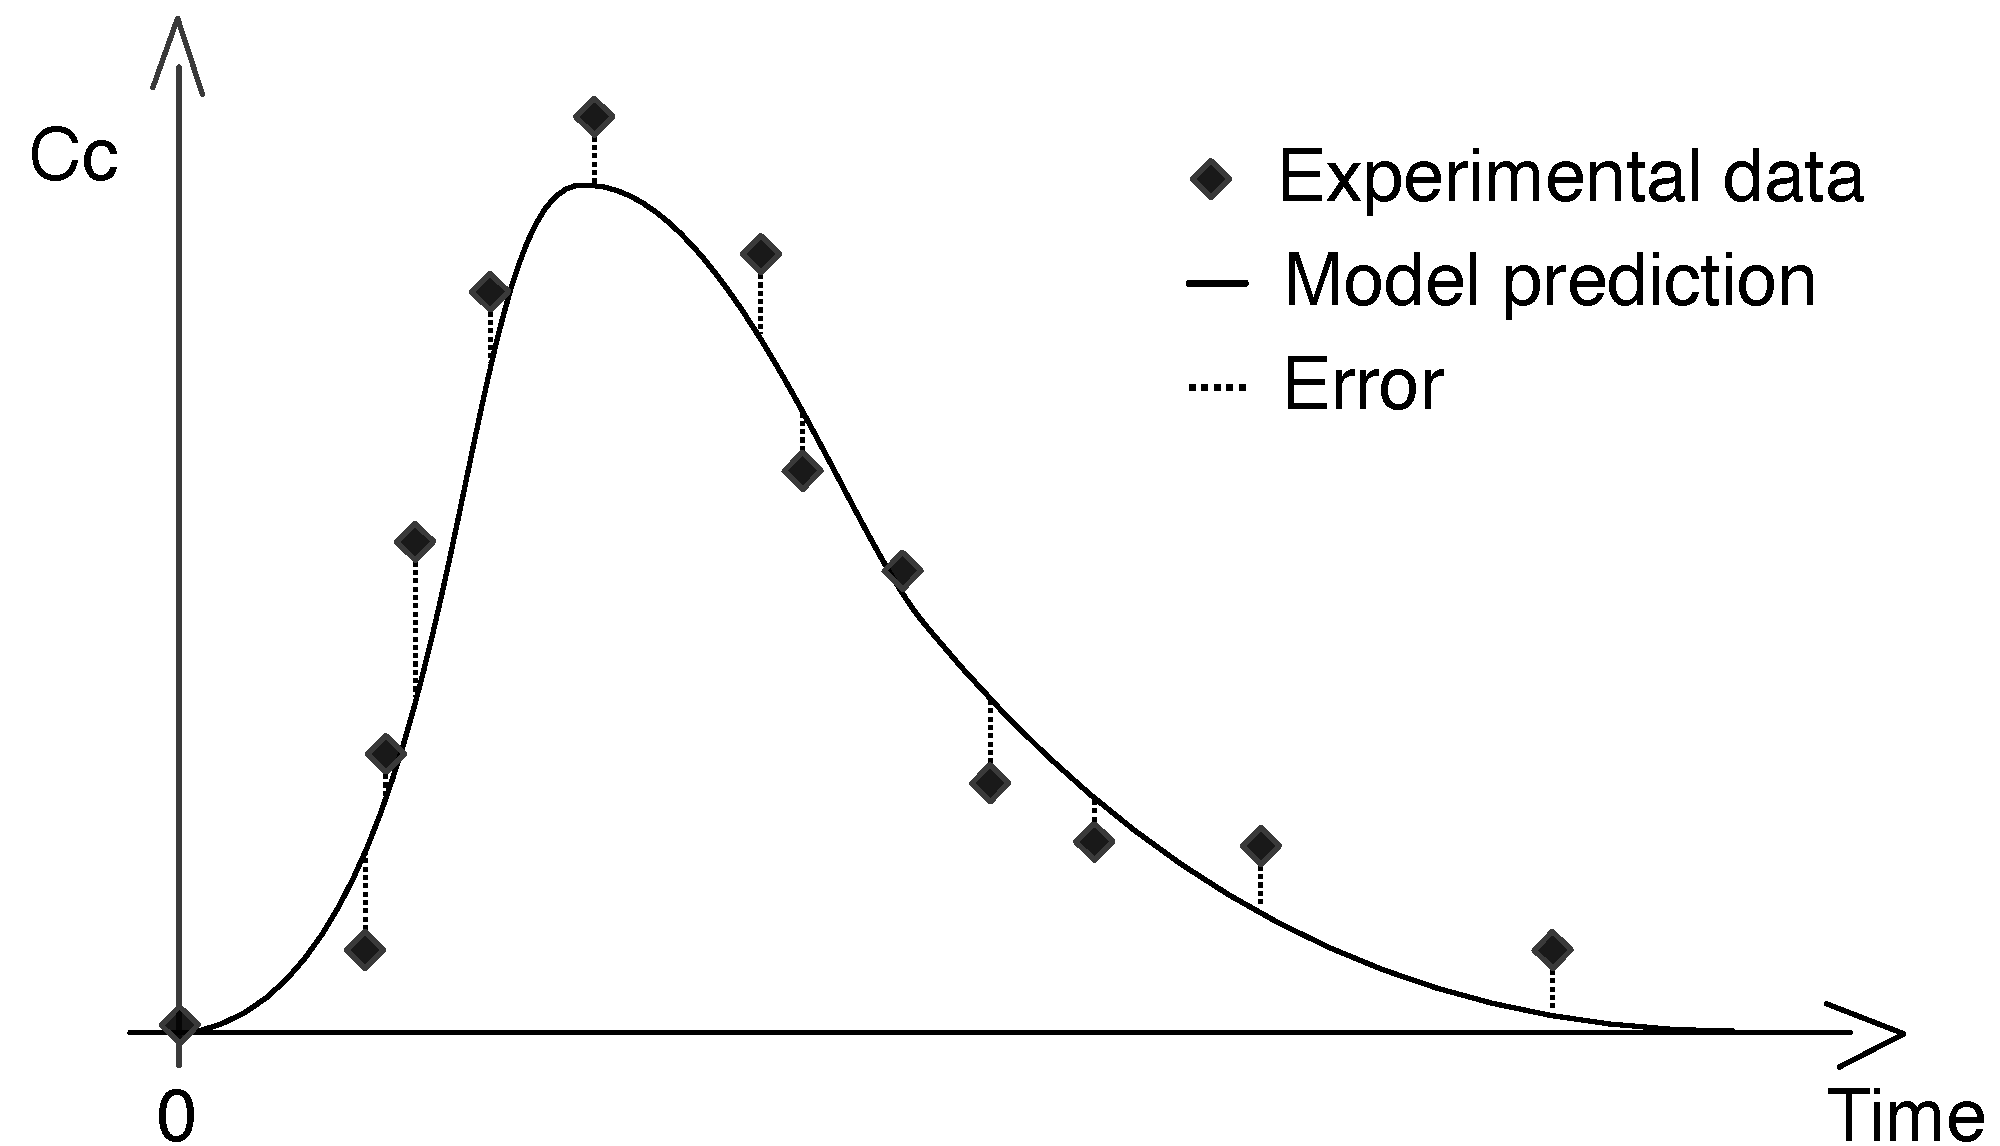
\includegraphics[height=45mm]{pics/Model-individual}
\caption{Frequently sampled individual PK data. The black diamonds stand 
for experimental data, the solid line for the time course of concentration as 
predicted by a mathematical model. }
\label{fig:indivModel}
\end{figure}

\begin{figure}[htbp]
\centering
 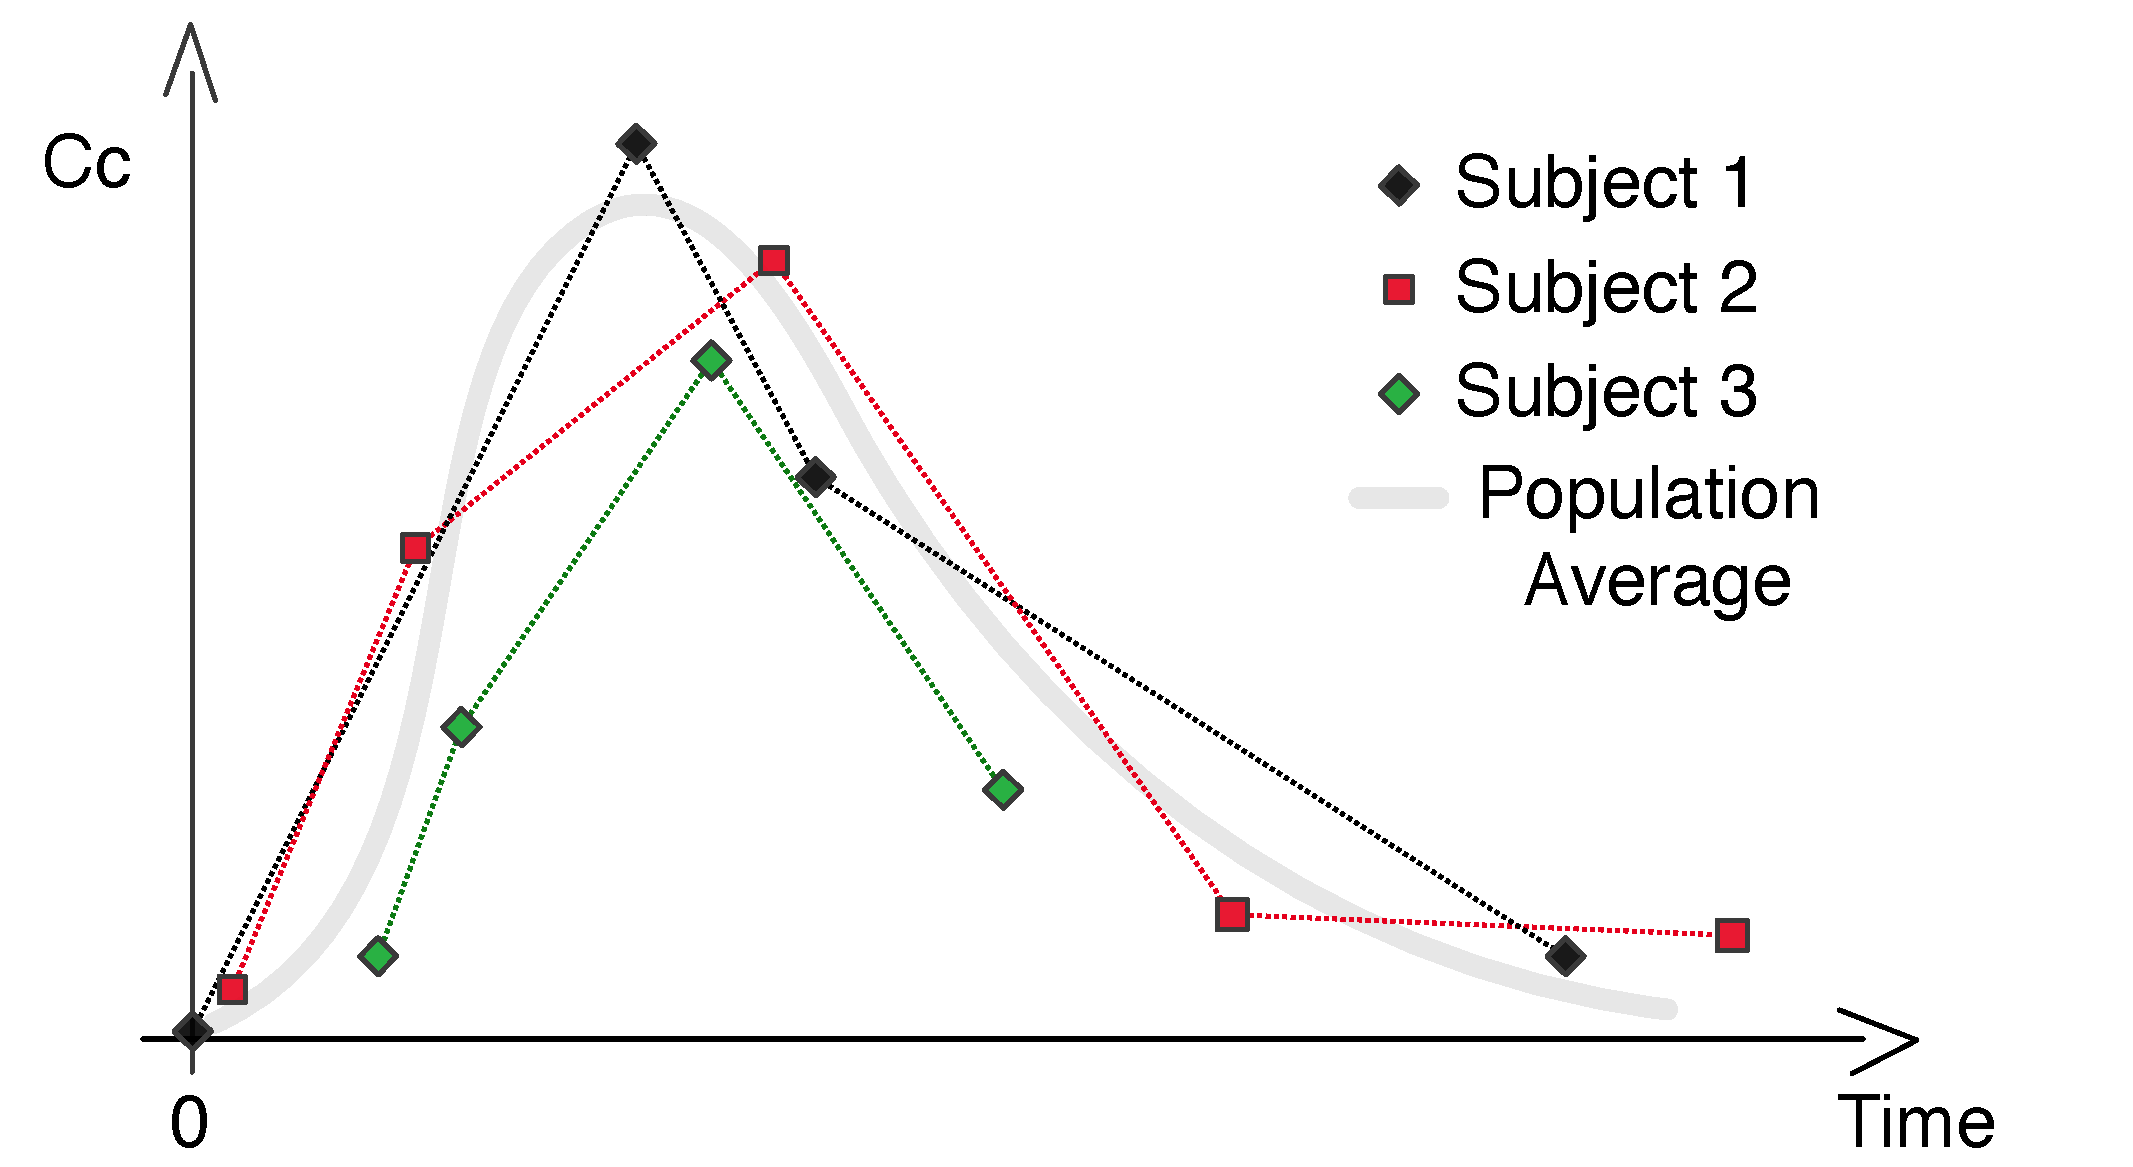
\includegraphics[height=45mm]{pics/Model-population}
\caption{Population PK data --  for three subjects with different observation times 
and varying characteristics, such as area under the curve, maximum values, 
time of the maximum etc. The grey line of the population average is to be 
estimated along with individual estimates.}
\label{fig:popModel}
\end{figure}

\section{Non-linear mixed effect models}\index{non-linear mixed effect models} 

The approach which proved to be very effective for the analysis of population 
data is that of \textbf{nonlinear mixed effect models}, NLME 
\cite{Bonate:2011fk,LavielleBook:2014}. 
The nonlinearity means that it can handle virtually any type of structural 
model, usually highly non-linear. Additionally one can consider population 
or subject related factors, known \emph{a priori} or collected during the 
study, which can be divided into two groups:
\begin{itemize}
\item
\textbf{fixed effects} -- population averages, e.g. typical/population value 
for volume, and other group or even subject specific explanatory variables, 
such as treatment groups, gender or weight, see covariate model in 
section \ref{maths:covariate_model}.\index{fixed effects}
\item
\textbf{random effects} -- subject/occasion specific, e.g. \textit{inter-individual} 
or \textit{inter-individual within subject within centre variability}, see section 
\ref{sec:variabilityModel} on variability.\index{random effects}
\end{itemize}
The notation of fixed versus random effects might be at first confusing as the 
former account for population, group but also subject characteristics. As 
explained in the parameter model section, the values of individual characteristics 
are subject specific features but the parameters assigned to them are identical 
for a group or population. \\
The structure of this chapter is the following, in section \ref{sec:continuousDataModel} 
we formulate a general nonlinear mixed effects model for continuous data, 
section \ref{sec:structuralModel} introduces the structural model, section 
\ref{sec:variabilityModel} discusses the variability as nested hierarchy, section 
\ref{sec:parameterModel} is about the parameter model, with discussion on 
correlation of random effects, covariate model and a comparison of equivalent 
representations of the parameter model and section \ref{sec:residualErrorModel} 
is about the residual error model. 
% and last section \ref{sec:CTS} about the trial design model.


\section{Continuous data model}\index{continuous data model}
\label{sec:continuousDataModel}
A general nonlinear mixed effects model for continuous data for $N$ subjects and $n_i$ measurements per subject $i$ reads as follows, \cite{LavielleBook:2014}:
\begin{align}
 \underbrace{ y_{ij}}_{\text{\parbox{2cm}{\centering Experimental \\[-4pt]  data}}} =
 \underbrace{ f(x_{ij}, \psi_{i})}_{\text{\parbox{2.5cm}{\centering Model \\[-4pt]  prediction}}} + 
 \underbrace{ g(x_{ij}, \psi_{i}, \xi) \; \epsilon_{ij}}_{\text{\parbox{3cm}{\centering Error}}} 
\quad 1\le i \le N, \quad 1\le j \le n_i \label{eq:nlmeModel}
 \end{align}
with
\begin{itemize}
\item
$y_{ij}$ -- $j^{th}$ observation for subject $i$
\item
$f$ -- structural model prediction
\item
$x_{ij}$ -- regression variables, e.g. $time$ or $concentration$
\item
$\psi_{i}$ -- individual parameters
\item
$\epsilon_{ij}$ -- residual error
\item
$g$ -- standard deviation of the residual error
\item 
$\xi$ -- parameters of the residual model
\end{itemize}
With $\epsilon_{ij}$ being normal distributed with mean 0 and variance 1, $y_{ij}$ is also normally distributed with mean $ f(x_{ij}, \psi_{i})$ and the standard deviation $g(x_{ij}, \psi_{i}, \xi)$. 


\section{Structural model}\index{structural model}
\label{sec:structuralModel}
This section deals with the first term of the right hand side in eq.\ref{eq:nlmeModel}
\begin{align*}
	f(x_{ij}, \psi_{i}) 
\end{align*}
i.e. the model prediction.

It can be formulated as a simple algebraic equation (e.g. Hill equation) or complex physiology-based PK model implemented as system of ODEs. When defined in such framework, this deterministic model for an individual will later be embedded in a statistical model. Other approaches, such as SDE-based structural models are not supported in this specification.\index{structural model!ordinary differential equations (ODE)}

%\begin{figure}[htbp]
%\begin{center}
%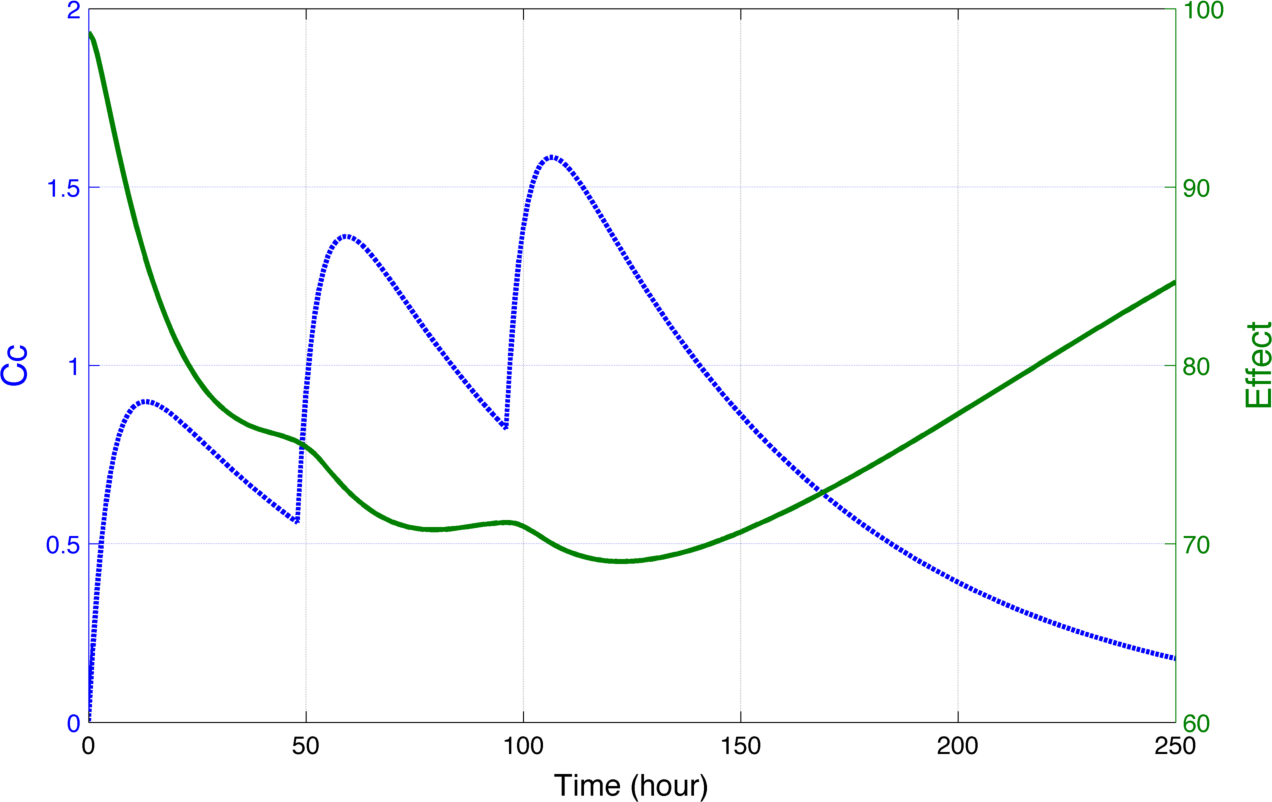
\includegraphics[width=.45\textwidth]{CTS1_smallPKPD}
%\caption{Simulated combined model as defined in the example with PK (blue) and PD (green) time courses for one subject. Here three doses were administered every $48h$.}
%\label{fig:simplePKPD}
%\vspace{-20pt}
%\end{center}
%\end{figure}
%  \vspace{-20pt}
%  \caption{A gull}
%  \vspace{-10pt}
%\end{wrapfigure}
\paragraph{Example}
As an example of a structural model we consider a combined PK/PD model, % see figure \ref{fig:simplePKPD},
\begin{itemize}
\item
PK -- oral one-compartmental model
\item
PD -- turnover model, so called $I_{max}$ model
\end{itemize}
with the following model parameters $ka$, $V$, $CL$, $Imax$, $IC50$, $Rin$ and $kout$.
\begin{align*}
k&=CL/V  \\
\frac{dAd}{dt} &=-ka\times Ad  \\
\frac{dAc}{dt}&=ka \times Ad - k \times Ac  \\
\frac{dE}{dt}&=Rin \times \Bigg(1-\frac{Imax \times Cc}{Cc+IC50}\Bigg) - kout \times E \\
\mbox{Initial condition: } & E(t=0) = Rin/kout   \\
& Ad(t=0) = DoseSize  \\
& Ac(t=0) = 0;  \\
Cc &= Ac/V  
\end{align*}

\paragraph{Alternative formulation 1}\index{structural model!analytic solution}
The PK model can, in this case, be formulated as an algebraic equation because an analytic solution exists, i.e.
\begin{align*}
C(t) = \frac{D}{V}  \frac{ka}{ka - k} \Big(e^{-k(t-t_D)} - e^{-ka(t-t_D)} \Big) 
\end{align*}

\paragraph{Alternative formulation 2}\index{structural model!PK macros}
PK macros offer an equation-free option to implement PK compartmental models.
For details see chapter\ref{sec:PKMacros}.

\subsection{Delayed Differential Equations (DDE)}\index{structural model!delayed differential equations (DDE)}
Additionally to the ODEs and algebraic equations, version \currpml of PharmML offers
the possibility to use Delayed Differential Equations. Similarly to initial conditions required
for an ODE, the so-called \emph{history} has to be defined. If a model is defined for times
$t \geq t_0$, the history specifies the values of the model variables for the 
time $\leq t_0$. 
The following simple example, from \cite{MLXTRANforMonolix:2014}, shows how 
such model and the according history can be formulated. 
\begin{align}
& \frac{dA}{dt} = r - c \times A \times B - k \times A \nonumber \\
& \frac{dB}{dt} = c \times A \times B - A(t-d) \nonumber 
\end{align}
with history $A_0 = r/k$ and $B_0 = 0$ for $t \le 5$. \emph{d} is the discrete delay parameter.

%
%\begin{eqnarray}
%\frac{d\textbf{y}(t)}{dt} &=& F(t,\textbf{y}(t)) \nonumber \\
%with  && \textbf{y}(t_0) = \textbf{y}_0  \nonumber
%\end{eqnarray}
%
%i.e. using explicit, first order ODEs.
%
%\paragraph*{Note on initial conditions}
%Some models have long algebraic expressions for every initial condition, e.g. here the value for glucose in liver:
%\begin{eqnarray}
%G_{L,0}=(1/Q_{G,L})*(Q_{G,A}*G_{H,0} + Q_{G,G}*G_{G,0} + Q_{G,PN}*G_{PN,0} + r_{B_{HGP}} - r_{B_{HGU}}) \nonumber
%\end{eqnarray}
%with 
%Initial conditions (defined/calculated before)
%\begin{eqnarray}
%&&G_{H,0} = a; \;\;\;G_{G,0} = b; \;\;\;G_{PN,0} = c; \quad with \quad a,b,c \in R \nonumber 
%\end{eqnarray}
%and other user defined functions
%\begin{eqnarray}
%&& r_{B_{HGP}} = f_1(y) \nonumber \\
%&& r_{B_{HGU}} = f_2(y) \nonumber
%\end{eqnarray}



\section{Nested hierarchy as the random variability structure}\index{variability model}\index{variability model!nested hierarchy}
\label{sec:variabilityModel}
\label{math:variability}

This section describes the variability structure of the random effects and the related naming 
convention. It is largely based on the discussions and conclusions from the DDMoRe 
Copenhagen focus 
meeting (Section \ref{sec:ddmoreMeetings}). Accordingly, in the following we will distinguish: 
\begin{itemize}
\item
(related to the observations) -- \textit{residual variability}, also known as \textit{intra-individual variability} and
\item
(related to the parameters) -- \textit{inter-individual} and \textit{inter-occasion variabilities}
\end{itemize}
The former is described in the section \ref{sec:residualErrorModel}, while the latter is described in this section.

\begin{figure}[htb!]
\centering
  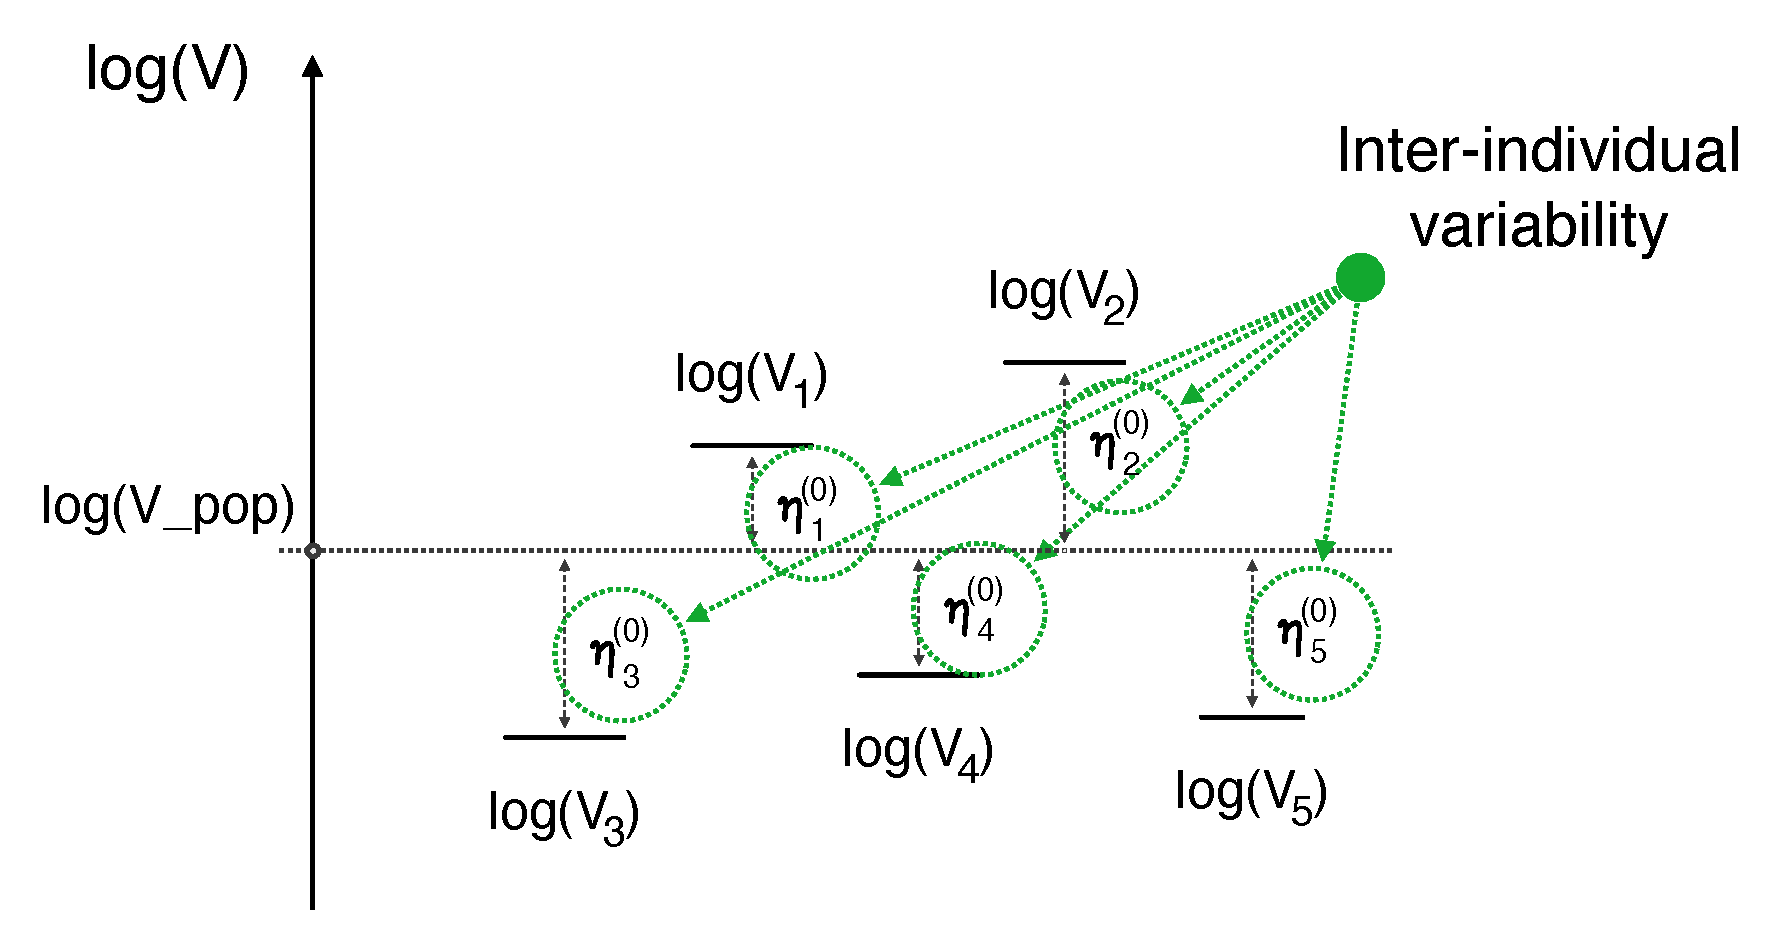
\includegraphics[width=95mm]{pics/Subject-level.pdf}
 \caption{Inter-individual variability typically occurring in an experiment, here $\log(V_{i=1\cdots5})$ 
 i.e. values for five subjects, varying around a typical value $\log(V_{pop})$, are shown.}
 \label{fig:subjectLevelVariability}
\end{figure}

\begin{figure}[htb!]\index{variability model!inter-individual variability (IIV)}
\centering
  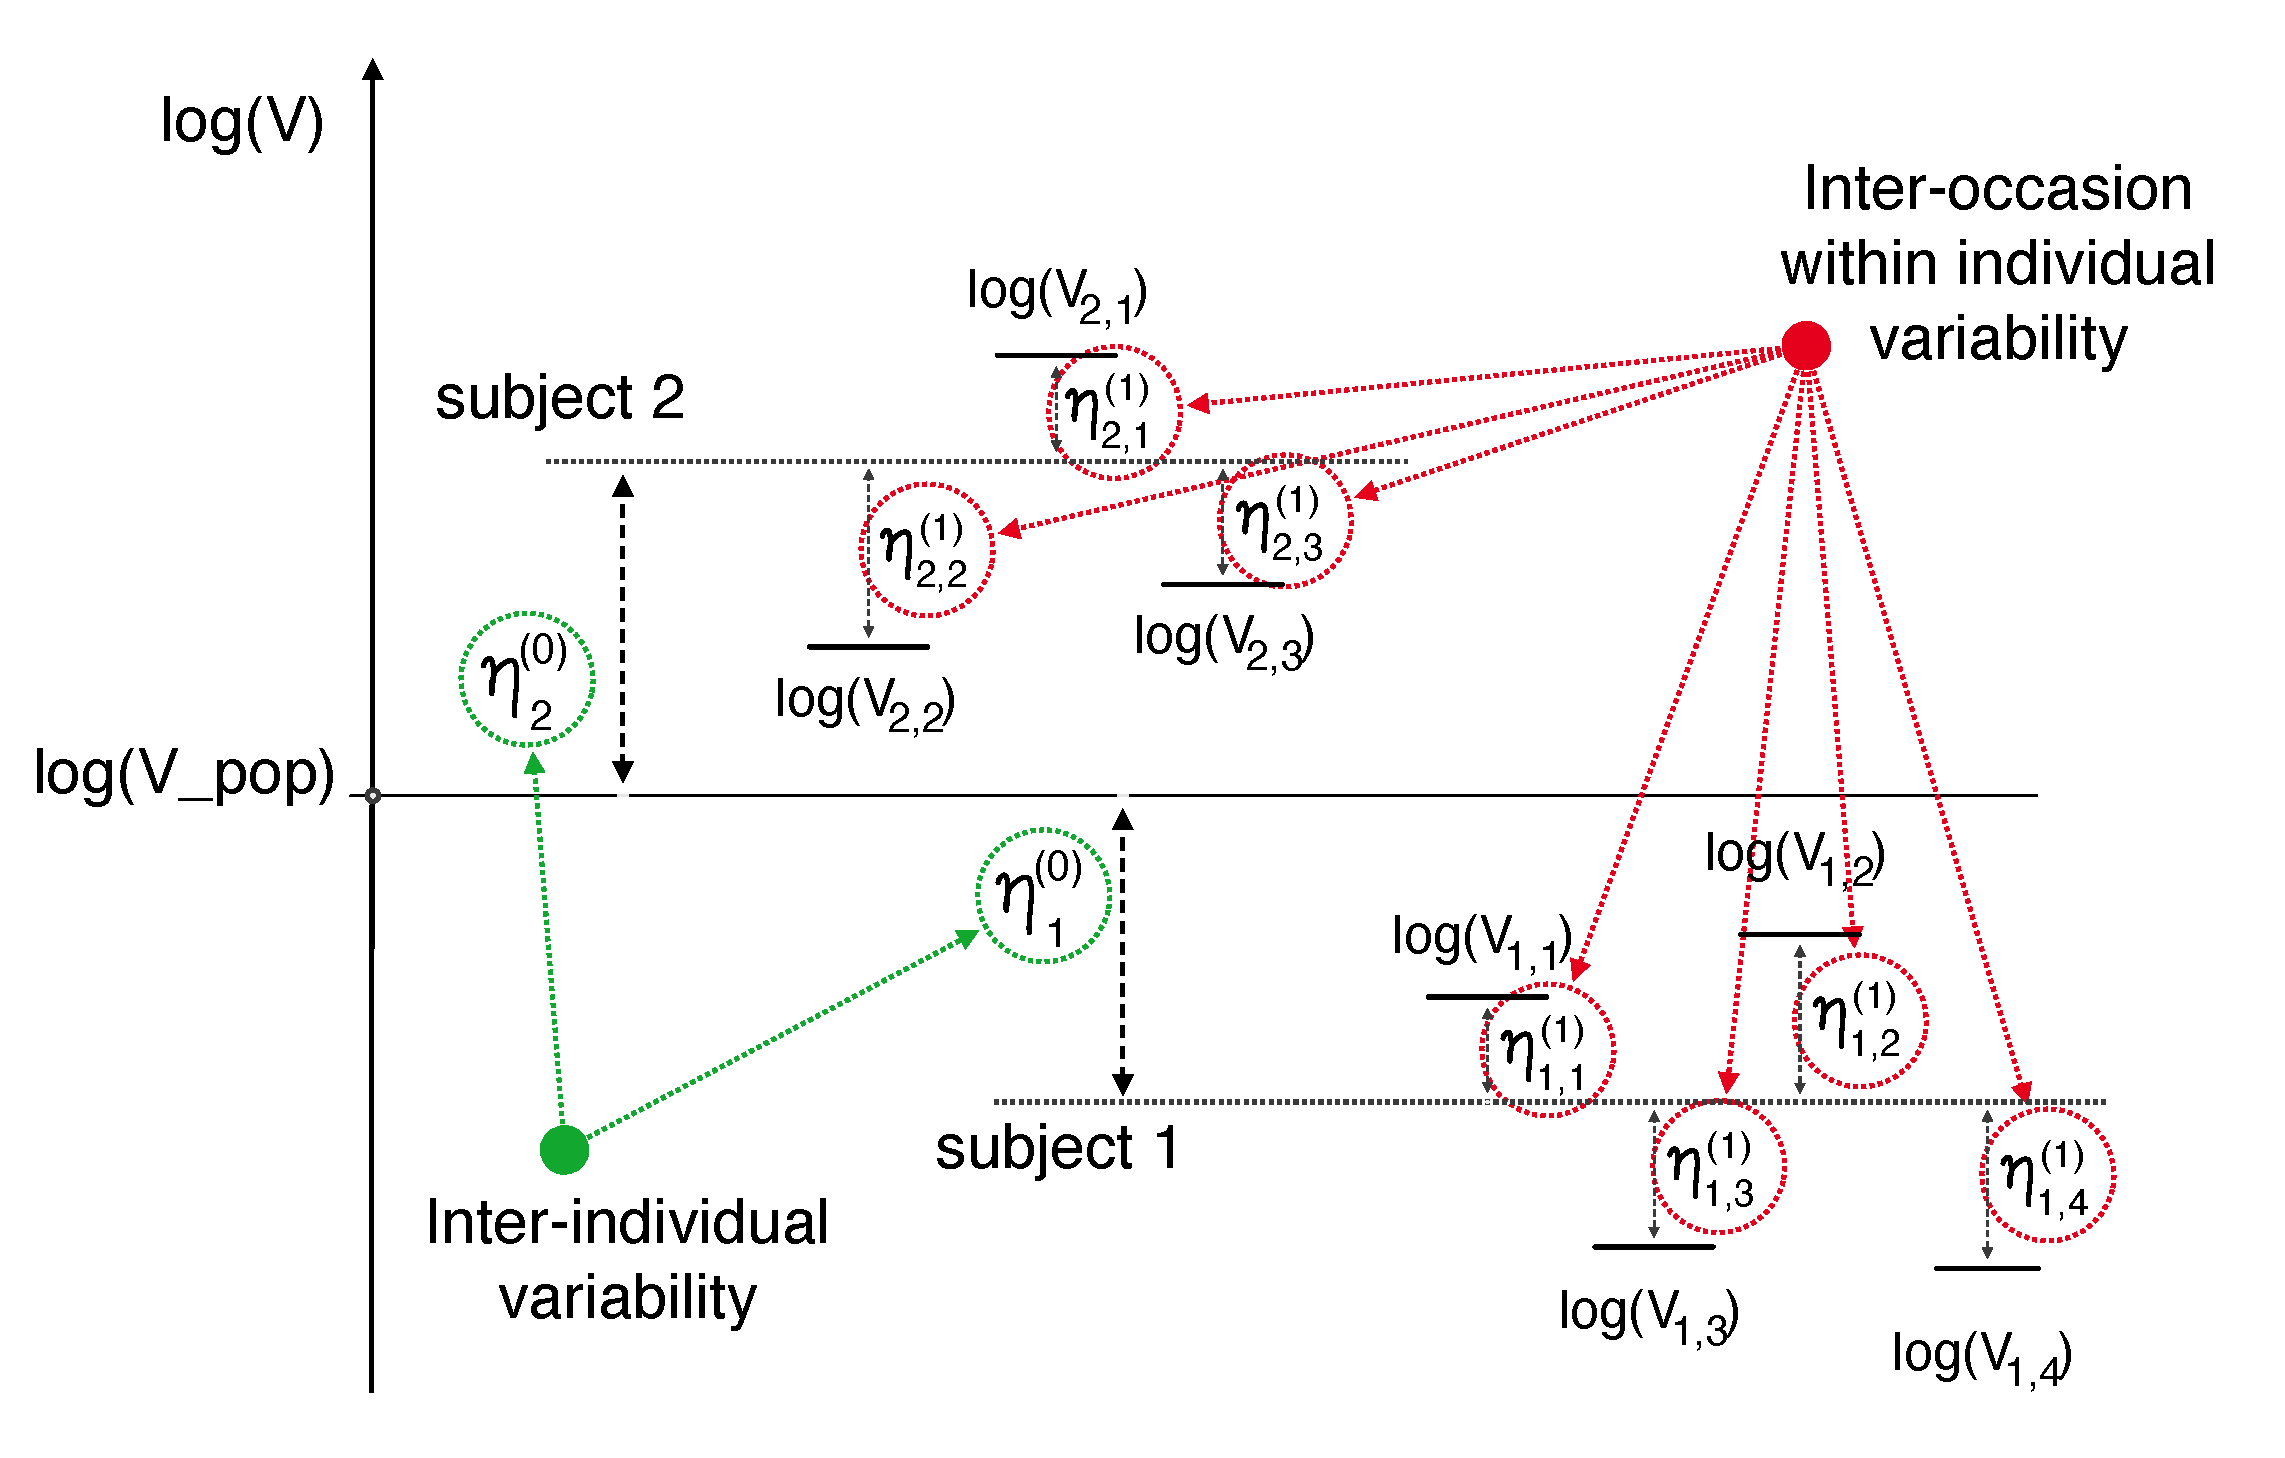
\includegraphics[width=120mm]{pics/Subject-occasion-level.pdf}
 \caption{Subject variability level, $(0)$, and within-subject (or occasion) variability level, $(1)$, typically occurring in an experiment, with index $i$ for subjects and $k$ for occasion. Here two subjects only are visualised, each of them having four or three occasions, respectively.}
 \label{fig:subjectOccasionLevelVariability}
\end{figure}

\subsection{Motivation}
One way to look at variability is to consider the following simple experiment: in this 
experiment, we estimate the volume of distribution in five subjects. Following a drug 
administration we collect blood samples over a time interval and estimate each 
subject's PK parameters. The result will be a set of five individual estimates such 
as those in Figure \ref{fig:subjectLevelVariability}. The values vary around a certain 
typical/population value. It is apparent that the only variability source is the fact that 
these are different persons, i.e. we have a rough estimate of the so called 
\textit{inter-individual} variability.\\
As an extension of this setup, we can now consider different number of occasions, 
when the PK parameters are estimated for each subject. If we restrict the discussion 
to two subjects only, each of them having three or four occasions, respectively, we 
can illustrate the results such those in Figure \ref{fig:subjectOccasionLevelVariability}. 
Repeatedly performing the same experiment for each subject is equivalent to create 
an additional level of variability, the \textit{inter-occasion within individual} variability.\\ 
Similarly, one can add e.g. 'country' or 'study centre' as new variability levels. 
If a clinical trial has been conducted in various countries or centres, it is reasonable 
to ask if the geographic location influences the outcome of the study. 

\subsection{General case}\index{variability model!inter-individual variability (IIV)}\index{variability model!inter-occasion variability (IOV)}
As a generalisation of the examples described above, one can derive the 
\textit{nested hierarchy} (also known as \textit{inclusion hierarchy}) of the variability 
structure of random effects. It can be visualised as a tree or alternatively using 
a Venn diagram, see Figures \ref{IOVgeneral_tree} and \ref{IOVgeneral_venn}. \\
The tree representation consists of \textit{nodes} and \textit{links} or \textit{edges}. 
It has the advantage that it visualises the whole structure explicitly from the top 
level, the \textit{root} node, down to lowest level of the variability. It provides 
immediate insights needed to understand or to verify the setup of a trial design. 
However, in case of a very complex structure, with high number of levels and/or 
subjects, it can become very large, making the tree difficult to represent in a typical 
document. It this case showing only partial branches will be more helpful, 
e.g. Figure \ref{IOVgeneral_tree}.\index{variability model!tree structure} 
On the contrary, the Venn diagram visualises 
the levels only, and it might be more suited for the complex cases.\index{variability model!Venn diagram} 
Usually, the variability structure consists of only one or two levels, e.g. \textit{individual} or 
\{\textit{individual}, \textit{occasion}\}, see examples below. 


The \textit{root}, i.e. the top node in the tree structure, stands for the population/typical 
value of a parameter. Following the current nomenclature, every subsequent variability 
level is either 'positive' or 'negative' dependent on its position relative to the reference 
'subject level', denoted as 0 -- the level 'zero'. Each level has a covariance matrix 
associated with it, i.e. 
\begin{itemize}
\item 
$\Omega^{-n}$ -- for levels above the reference level -- their names will vary according to 
the nature of the levels. For example the variability on country level is called 
'between-country variability'.
\item 
$\Omega^0$ -- reference level\footnote{Target tools such as NONMEM or Monolix assume 
the subject level as the reference level by default. \pml doesn't make such assumption and 
the \emph{zero} level can be explicitly defined and is required if more then one level exist.}, 
also called BSV (between subject variability) or IIV (inter-individual variability).
\item 
$\Omega^{+n}$ -- for levels below the reference level -- called  IOV (inter-occasion variability) or
WSV (within-subject variability).
\end{itemize}
The number of levels will vary dependent on the nature of the study. Cases without or 
with only positive/negative levels are possible. Please note that \pharmml doesn't require 
numbers to be assigned to the various levels of variability. Instead the user can 
define meaningful identifiers.

\begin{figure}[htb!]
\centering
  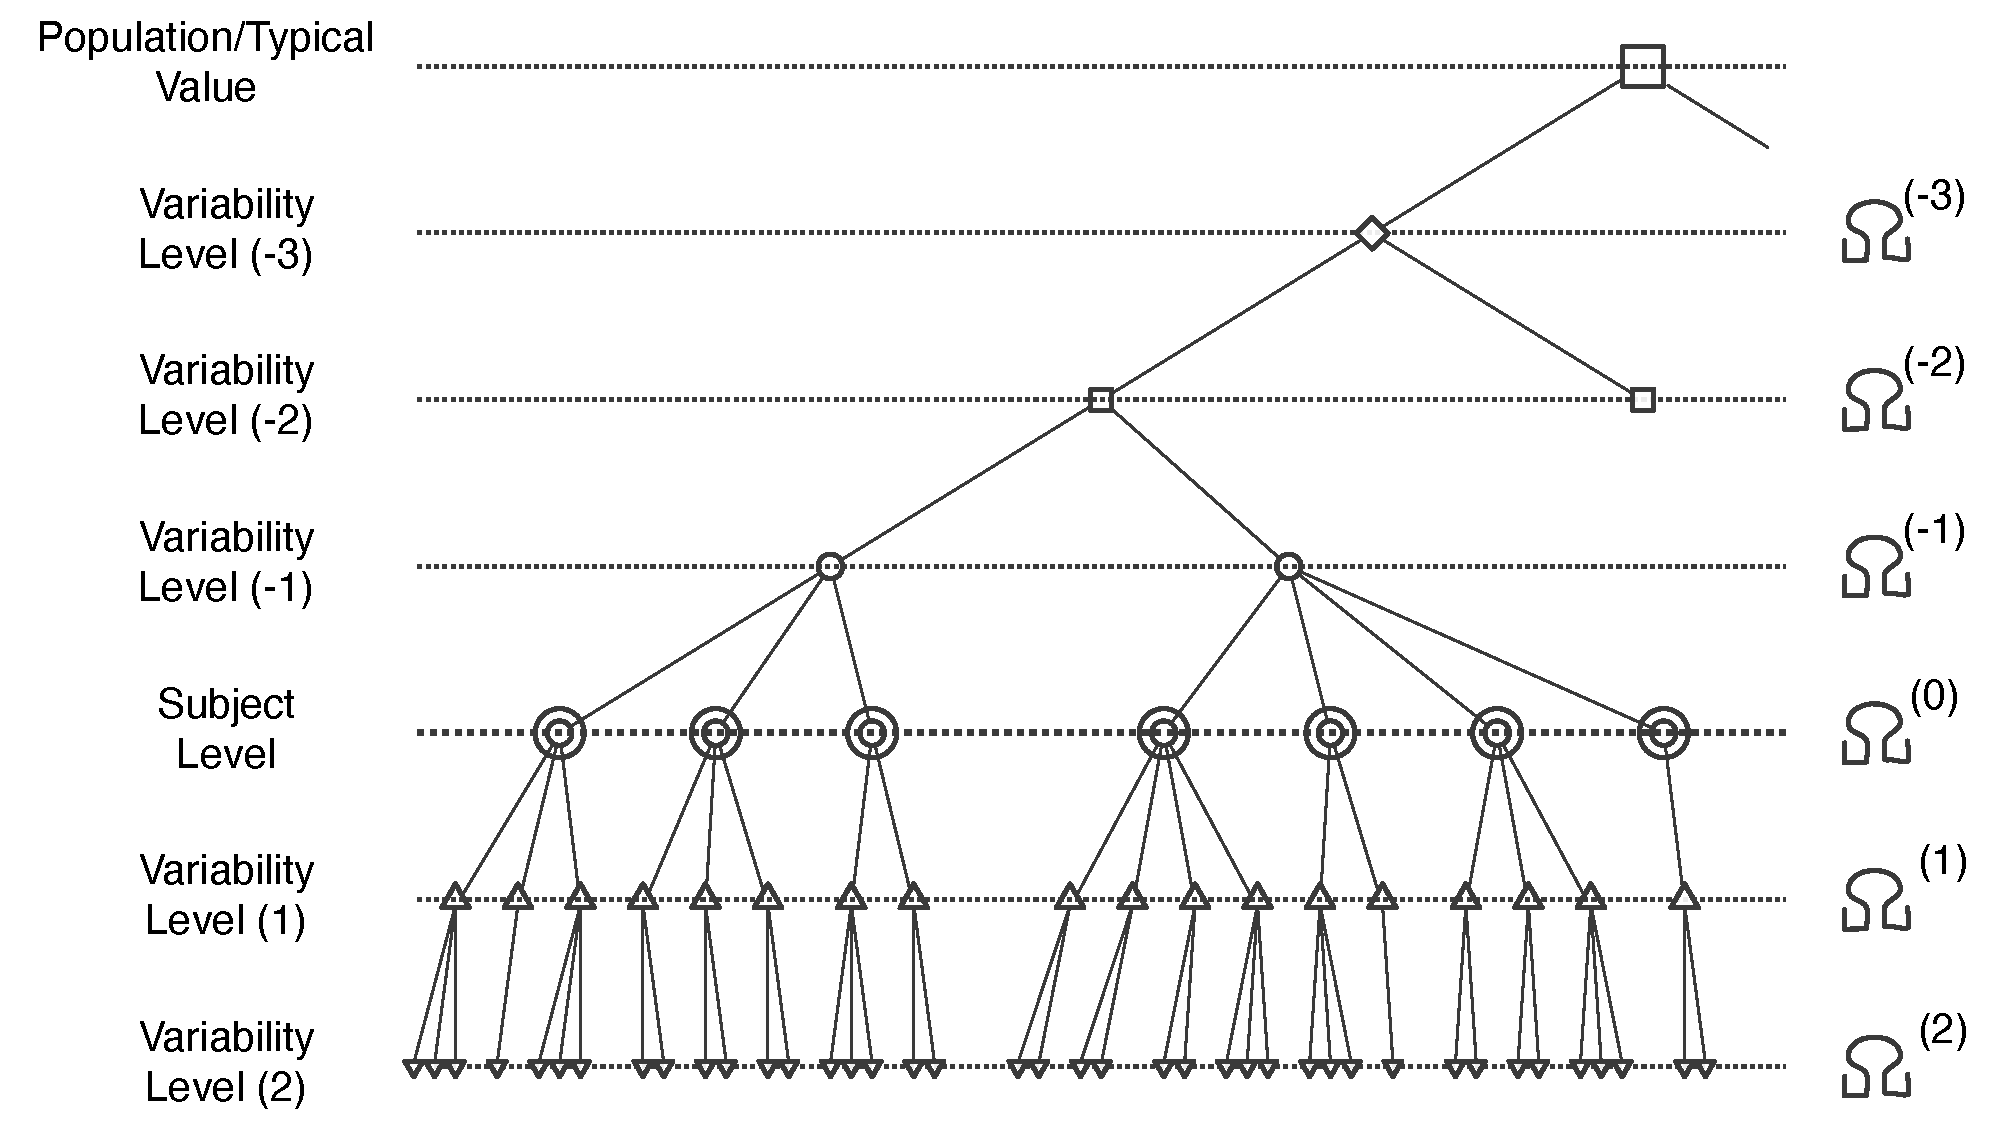
\includegraphics[width=130mm]{pics/IOV-general-TREE}
 \caption{General nested hierarchy of the variability structure -- as tree. Note that 
 \pharmml doesn't require or use numbers to be assigned to the various levels of 
 variability. Instead the user can define meaningful identifiers such as \emph{subject}
  or \emph{iiv} for level (0), \emph{occasion} or \emph{iov} for level (1), \emph{study} for level (-1) etc.}
 \label{IOVgeneral_tree}
\end{figure}

\begin{figure}[htb!]
\centering
  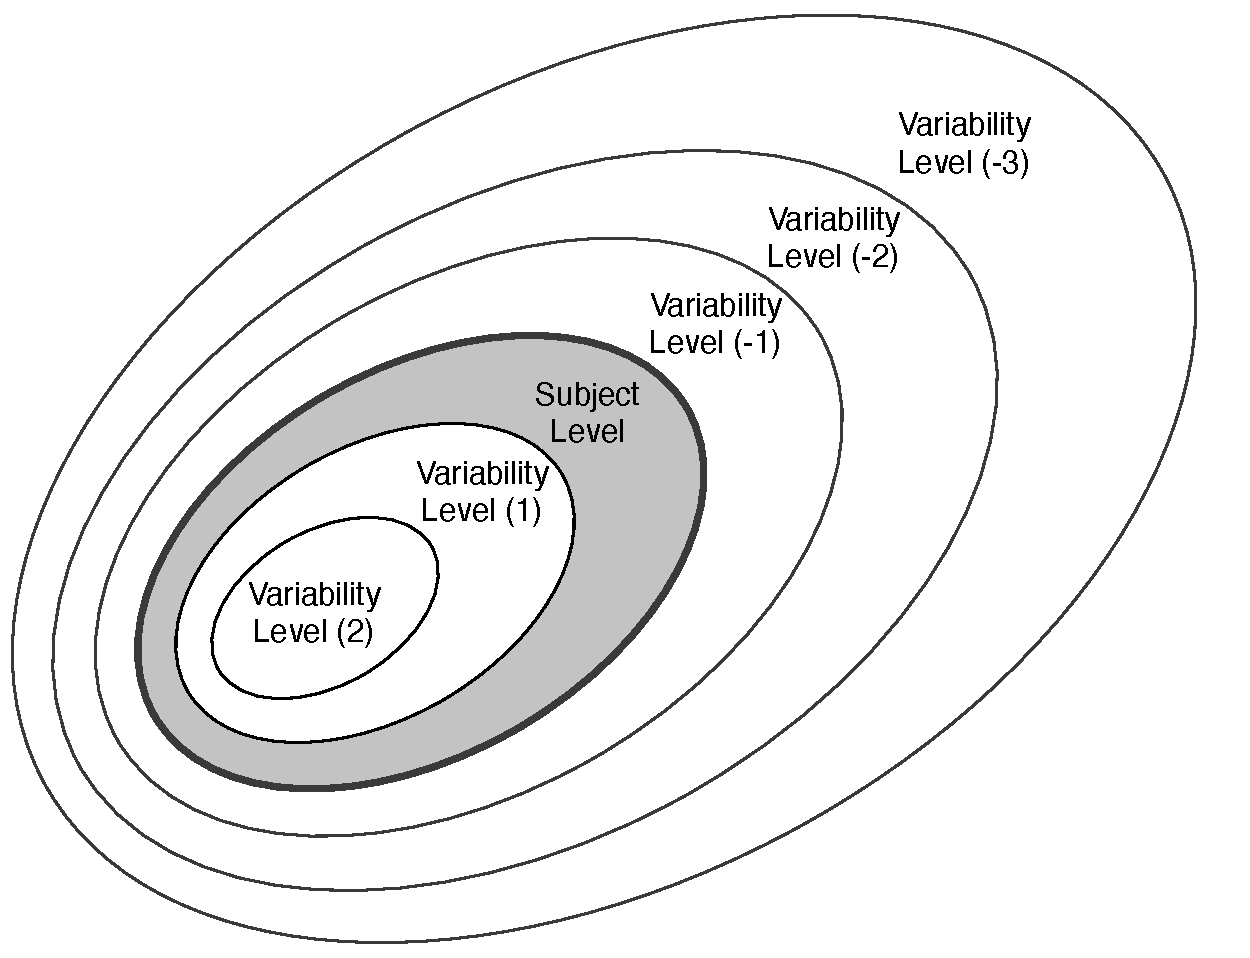
\includegraphics[width=90mm]{pics/IOV-general-VENN}
 \caption{General nested hierarchy of the variability structure -- as Venn diagram.}
 \label{IOVgeneral_venn}
\end{figure}


\paragraph{Example 1}\index{variability model!examples}
This example handles the simplest scenario, with only one level of variability: \textit{subject}--level, see Figure \ref{tree_IOV0}. The following symbols are used
\begin{itemize}
\item
$i$ -- subject index, $1\le i \le N$
\end{itemize} 
with $N_l$ -- number of subjects.\\
The typical parameter model, without covariate, reads as follows:
\begin{align*}
& \log(V_i) = \log(V_{pop}) + \eta_i^{(0)}  
\end{align*} 
or alternatively:
\begin{align*}
& V_i = V_{pop} \,e^{\eta_i^{(0)}}  
\end{align*} 
with $\eta_i^{(0)} \sim \mathcal{N}\big(0,\Omega^{(0)}\big)$.


\begin{figure}[htb!]
\centering
  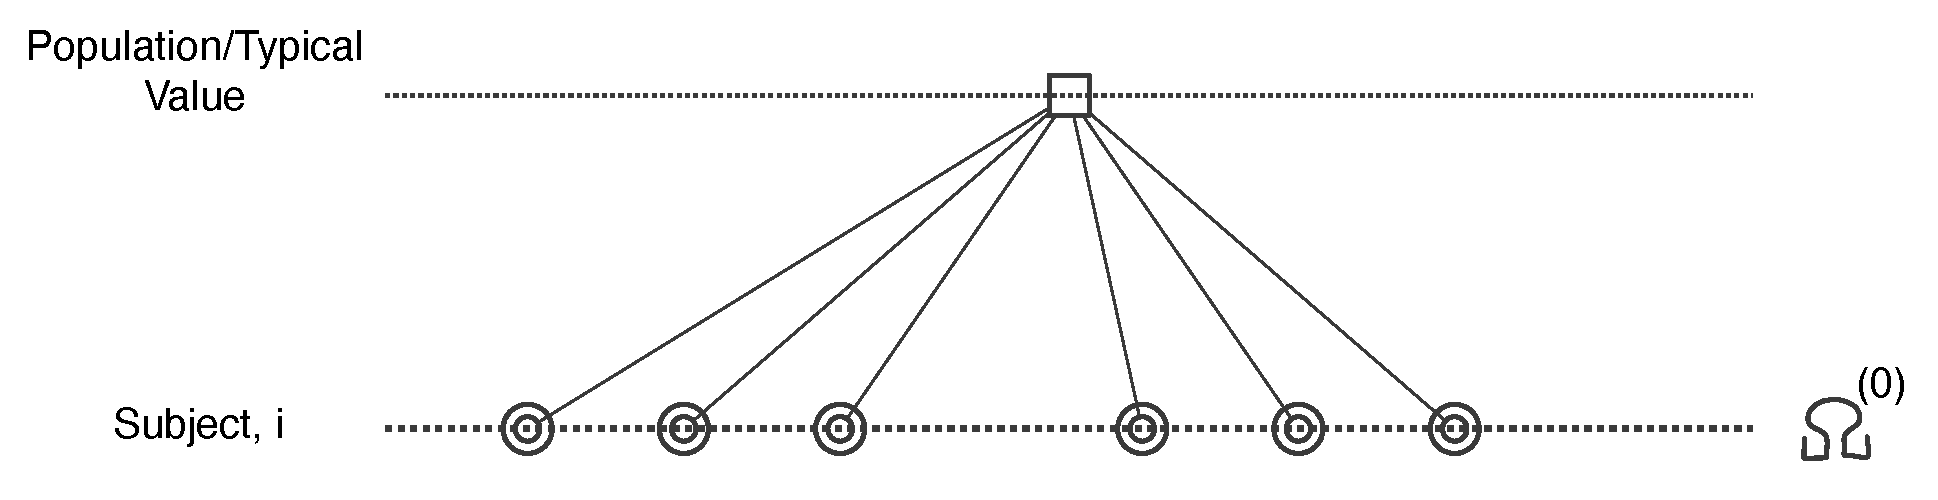
\includegraphics[width=120mm]{pics/tree_IOV0}
 \caption{Example 1 -- single level of variability: \textit{subject} -- (0) level.}
 \label{tree_IOV0}
\end{figure}

\paragraph{Example 2}\index{variability model!examples}
In this example there are three levels of variability: \{\textit{centre, subject, occasion}\}, see Figure \ref{tree_IOV1}. Following symbols are used:
\begin{itemize}
\item
$l$ -- centre index, $1\le l \le L$
\item
$i$ -- subject index, $1\le i \le N_l$
\item
$k$ -- occasion index, $1\le k \le N_{li}$
\end{itemize} 
with
\begin{itemize}
\item
$L$ -- number of centres
\item
$N_l$ -- number of subjects in centre \textit{l}
\item
$N_{li}$ -- number of occasions in subject \textit{i} in centre \textit{l}
\end{itemize} 
The parameter model, without covariate, reads as follows:
\begin{align*}
& \log(V_{lik}) = \log(V_{pop}) + \eta_l^{(-1)} + \eta_{li}^{(0)} + \eta_{lik}^{(+1)}  
\end{align*} 
or alternatively:
\begin{align*}
& V_{lik} = V_{pop} \, e^{\eta_l^{(-1)}} e^{\eta_{li}^{(0)}} e^{\eta_{lik}^{(+1)}}  
\end{align*} 
with
\begin{align*}
 & \eta_l^{(-1)} \sim \mathcal{N}\big(0,\Omega^{(-1)}\big), \quad \eta_{li}^{(0)} \sim \mathcal{N}\big(0,\Omega^{(0)}\big),
\quad \eta_{lik}^{(+1)} \sim \mathcal{N}\big(0,\Omega^{(+1)}\big) 
\end{align*}


\begin{figure}[htb!]
\centering
  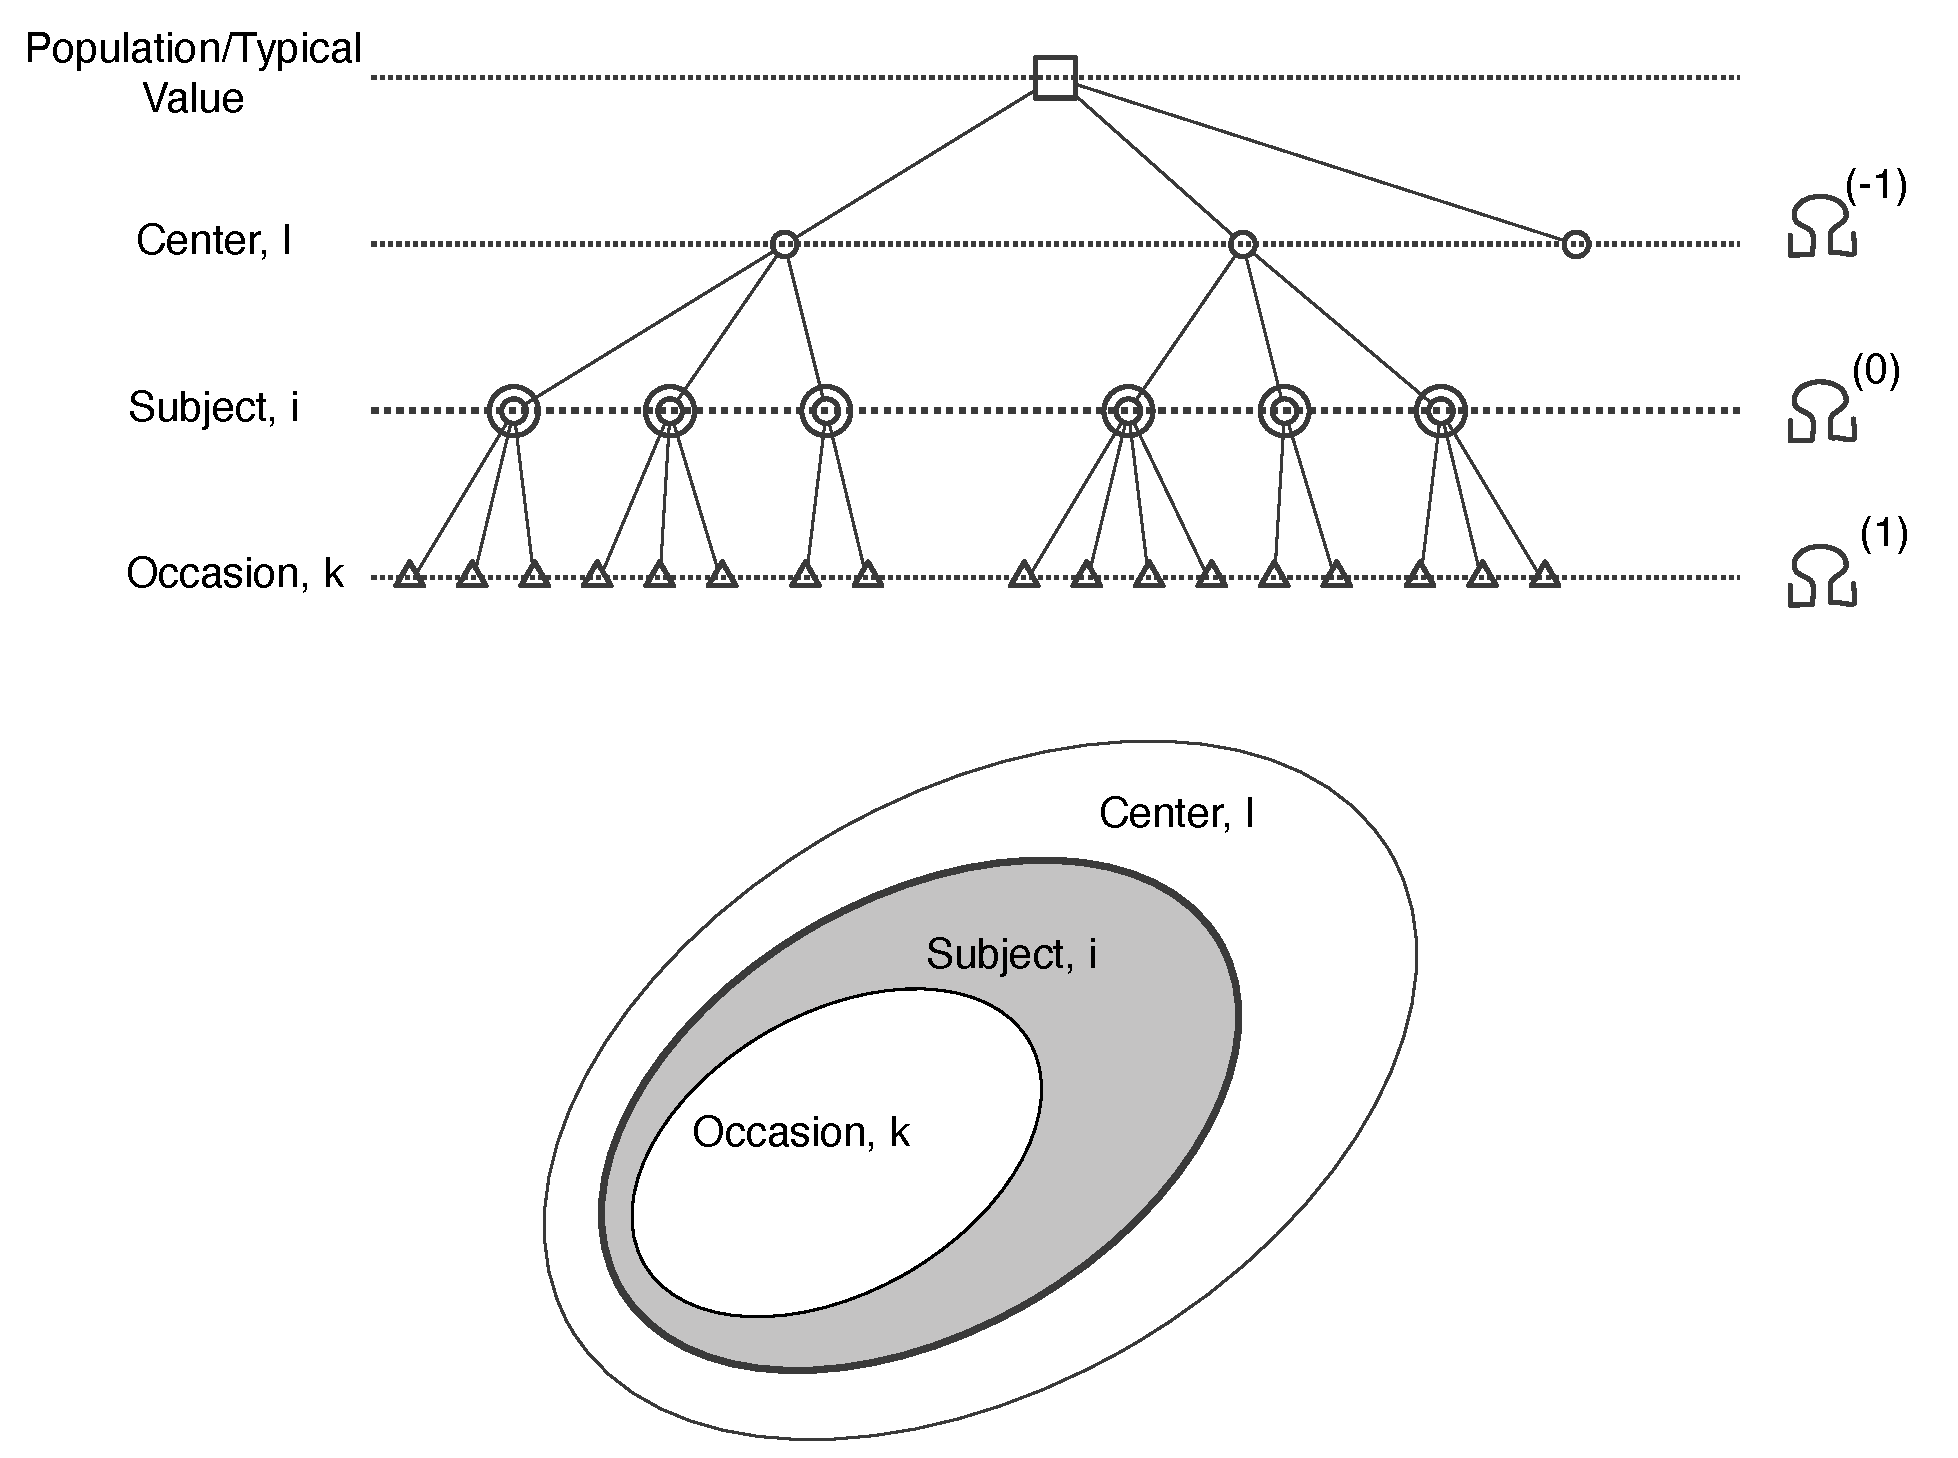
\includegraphics[width=120mm]{pics/tree_IOV1}
 \caption{Example 1 -- three levels of variability: \{\textit{centre (+1), subject (0), occasion (-1)}\}}
 \label{tree_IOV1}
\end{figure}


\paragraph{Example 3}\index{variability model!examples}
In this example there are four levels of variability: \{\textit{country, centre, subject, occasion}\}, see Figure \ref{tree_IOV2}. The symbol list is extended by one for 'country' as follows:
\begin{itemize}
\item
$m$ -- country index, $1\le m \le M$
\item
$l$ -- centre index, $1\le l \le N_m$
\item
$i$ -- subject index, $1\le i \le N_{ml}$
\item
$k$ -- occasion index, $1\le k \le N_{mli}$
\end{itemize} 
with
\begin{itemize}
\item
$M$ -- number of countries
\item
$N_m$ -- number of centres in country \textit{m}
\item
$N_{ml}$ -- number of subjects in centre \textit{l} in country \textit{m}
\item
$N_{mli}$ -- number of occasions in subject \textit{i} in centre \textit{l} in country \textit{m}
\end{itemize} 
The parameter model reads as follows:
\begin{align*}
& \log(V_{mlik}) = \log(V_{pop}) + \eta_m^{(-2)} + \eta_{ml}^{(-1)} + \eta_{mli}^{(0)} + \eta_{mlik}^{(+1)}  
\end{align*} 
or alternatively:
\begin{align*}
& V_{mlik} = V_{pop} \, e^{\eta_m^{(-2)}} e^{\eta_{ml}^{(-1)}} \; e^{\eta_{mli}^{(0)}} \; e^{\eta_{mlik}^{(+1)}}  
\end{align*} 
with
\begin{align*}
 & \eta_m^{(-2)} \sim \mathcal{N}\big(0,\Omega^{(-2)}\big), \quad \eta_{ml}^{(-1)} \sim \mathcal{N}\big(0,\Omega^{(-1)}\big), \quad
 \eta_{mli}^{(0)} \sim \mathcal{N}\big(0,\Omega^{(0)}\big), \quad \eta_{mlik}^{(+1)} \sim \mathcal{N}\big(0,\Omega^{(+1)}\big) 
\end{align*} 



\begin{figure}[htb!]
\centering
  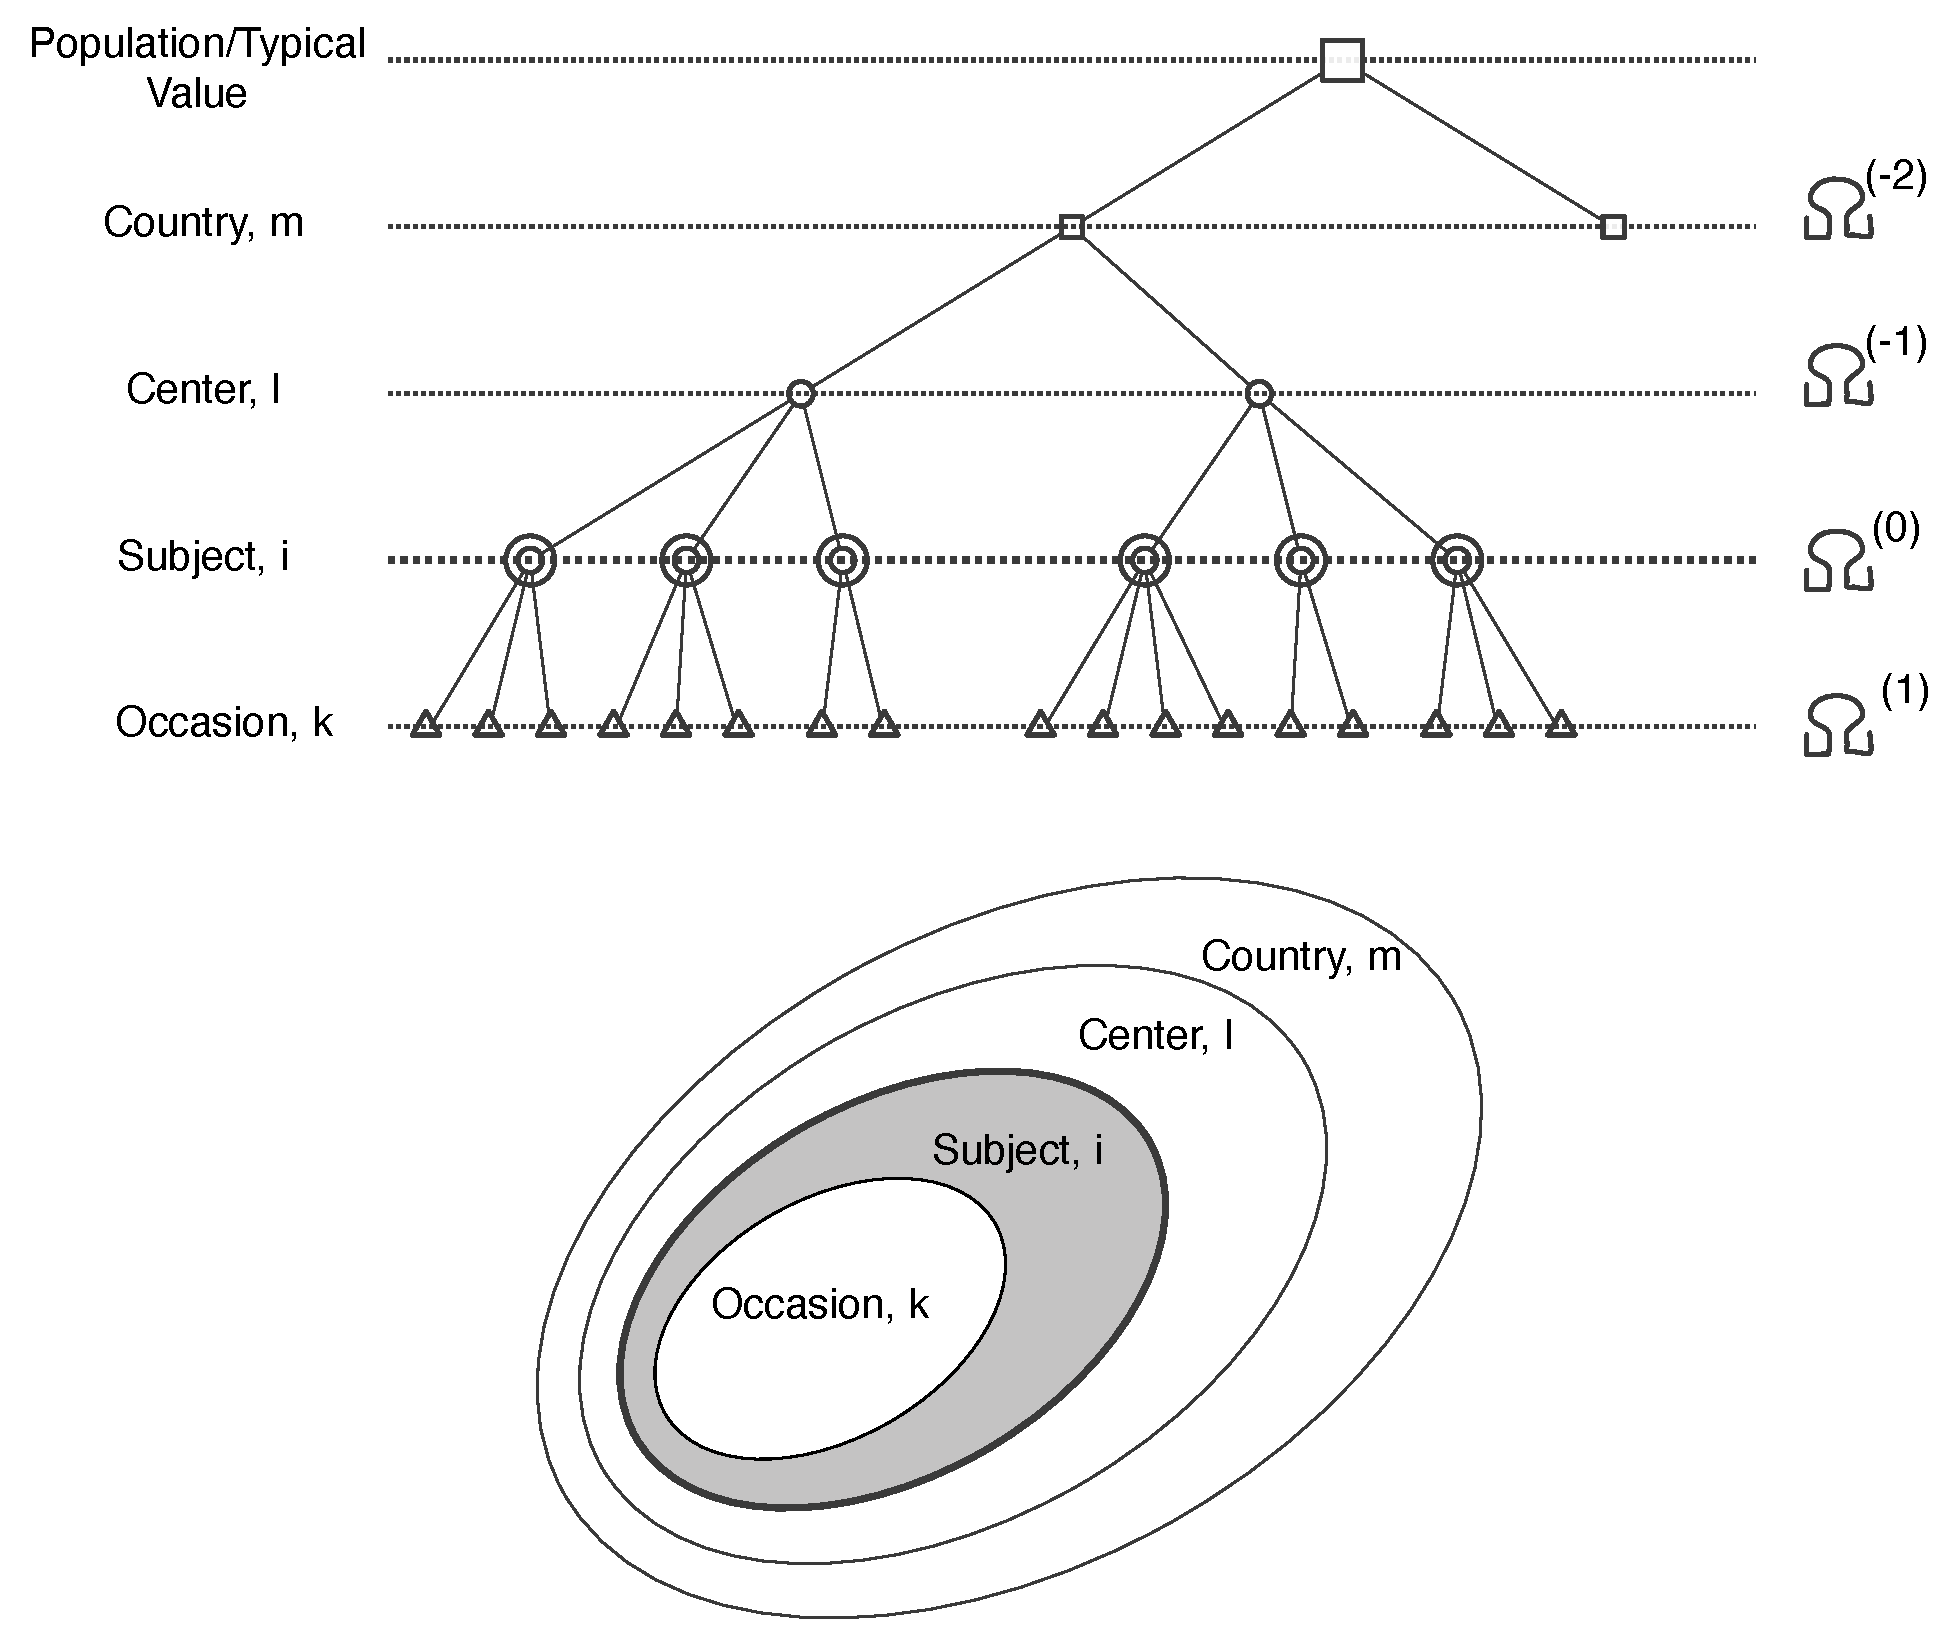
\includegraphics[width=120mm]{pics/tree_IOV2}
 \caption{Example 2 -- four levels of variability:  \{\textit{country (-2), centre (-1), subject (0), occasion (+1)}\}}
 \label{tree_IOV2}
 \end{figure}



\section{Parameter model}
\label{sec:parameterModel}
\label{maths:parameter_defn}
\label{maths:parameter-model}

The following section outlines the parameter model. We consider three types of parameter model:
\begin{itemize}
\item
Type 1. Implicit model \index{parameter model!implicit model}
\begin{align*}
\psi_i = H(\beta, C_i, \eta_i)
\end{align*}
This is the most general form of a parameter model with no constraints on the function $H$.
It is an implicit equation as it doesn't allow an easy interpretation of its elements in contrast to the two following forms.
\item
Type 2. Gaussian model with general covariate model \index{parameter model!Gaussian model!non-linear covariate model}
\begin{align*}
h(\psi_i) = H(\beta, C_i) + \eta_i
\end{align*}
Here the parameter is normally distributed up to a transformation $h$ with a general covariate model and additive random effects.
\item
Type 3. Gaussian model with linear covariate model \index{parameter model!Gaussian model!linear covariate model}
\begin{align*}
h(\psi_i) = h(\psi_{pop}) + \beta \, C_i + \eta_i
\end{align*}
This is a special case of the models above which allows for the most detailed interpretation as explained in the following section.
\end{itemize}
with
\begin{itemize}
\item
$\psi_i$ -- individual parameter
\item
$\psi_{pop}$ -- typical or population mean parameter
\item
$\eta_i$ -- random effect(s)
\item
$\beta$ -- fixed effect(s)
\item
$C_i$ -- covariate(s)
\item
H -- arbitrary function
\item
h -- function which transforms the model on both sides, e.g. log, logit, probit.
\end{itemize}

\subsection{Discussion and examples of Type 1 models}\index{parameter model!implicit model}
\label{subsec:paramModelType1}
This model type is the most flexible one, able to accommodate
\begin{itemize}
\item
multiple fixed effects
\item
multiple random effects and
\item
an arbitrary (nonlinear) covariate model.
\end{itemize}

\paragraph{Example}
Let's consider a complex clearance model as introduced in \cite{NONMEM:2006aa}, which contains
\begin{itemize}
\item
four fixed effects $\theta_1, \cdots, \theta_4$
\item
three continuous covariates $WT, AGE, SECR$
\item
one categorical covariate $ICU$
\item
three random effects $\eta_{1i,met}\sim \mathcal{N}(0,\omega_{1,met}^2),\eta_{2i,met}\sim \mathcal{N}(0,\omega_{2,met}^2), \eta_{3i,ren}\sim \mathcal{N}(0,\omega_{3,ren}^2)$
\end{itemize}
The model is composed of
\begin{enumerate}
\item
the average metabolic clearance which reads
\begin{align*}
& CL_{met_{average}} = WT\times \frac{\theta_1 - \theta_2 \times Cpss_2}{\theta_3 + Cpss_2}
\end{align*}
extended with random effects representing a patient being from an ICU (intensive care unit) or else
\begin{align*}
& CL_{i,met} = CL_{met_{average}} + (1 - ICU) \; \eta_{1,i} + ICU \; \eta_{2,i}
\end{align*}
i.e.
\begin{align*}
& CL_{i,met} = \left\{ \begin{array}{lcl}  CL_{met_{average}} + \eta_{1,i}  & \mbox{for} & ICU = 0 \quad \text{i.e. patient not from ICU} \\
CL_{met_{average}} + \eta_{2,i}  & \mbox{for} & ICU = 1 \quad \text{else}
\end{array}\right.
\end{align*}
\item
and average renal clearance which reads
\begin{align*}
& CL_{ren_{average}} = \theta_4 \times RF \quad \text{with}  \quad
RF = WT\times \frac{1.66 - 0.011 \times AGE}{SECR}
\end{align*}
so the clearance for subject $i$ amounts to
\begin{align*}
& CL_{i,ren} = CL_{ren_{average}}(1+ \eta_{3,i})
\end{align*}
\end{enumerate}
The complete model, combining (1) and (2), for an individual's clearance then reads
\begin{align*}
& CL_i = CL_{i,met} + CL_{i,ren}.
\end{align*}
This model, although fully flexible, is difficult to break into meaningful sub-components. This is an entirely different situation for the following model types, where clearly defined sub-components can be separately stored and annotated.
%\begin{itemize}
%\item
%metabolic clearance
%\begin{align*}
%& CL_{met_{average}} = WT\times \frac{\theta_1 - \theta_2 \times Cpss_2}{\theta_3 + Cpss_2}
%\end{align*}
%extended with random effects representing a patient being from an ICU (Intensive Care Unit) or else
%\begin{align*}
%& CL_{met} = CL_{met_{average}} + (1 - ICU) \, \eta_{1i,met} + ICU \, \eta_{2i,met}
%\end{align*}
%i.e.
%\begin{align*}
%& CL_{met} = \left\{ \begin{array}{lcl}  CL_{met_{average}} + \eta_1  & \mbox{for} & ICU = 0 \quad \text{i.e. patient not from ICU} \\
%CL_{met_{average}} + \eta_2  & \mbox{for} & ICU = 1 \quad \text{else}
%\end{array}\right.
%\end{align*}
%\item
%and renal clearance
%\begin{align*}
% CL_{ren} = \theta_4 \times RF
%\end{align*}
%with
%\begin{align*}
%& RF = WT\times \frac{1.66 - 0.011 \times AGE}{SECR}
%\end{align*}
%with covariates \var{WT}, \var{AGE} and \var{SECR}.
%\end{itemize}
%The complete model for an individual's clearance reads
%\begin{align*}
%& CL_i = CL_{met} + CL_{ren}\; \eta_{3i,ren}.
%\end{align*}

\subsection{Discussion and examples of Type 2 models}\index{parameter model!Gaussian model!non-linear covariate model}
\label{subsec:paramModelType2}
Here, we consider normally distributed parameters, up to a transformation $h$, i.e. normal, log-normal or logit-normally distributed with identity, the natural logarithm or the logit as transformation, respectively.

Compared to the Type 1 parameter model, the Type 2 parameter model has a more structured additive form:
\begin{align*}
h(\psi_i) =
\underbrace{H(\beta, C_i)}_{\text{\parbox{2.5cm}{\centering non-linear covariate\\[-4pt] model}}}
+ \underbrace{\eta_i^{(0)}+ \eta_{ik}^{(+1)} + \dots}_{\text{\parbox{3cm}{\centering IIV and other\\[-4pt] levels of variability}}}
\end{align*}
Accordingly a model for an individual parameter consists of
\begin{itemize}
\item
the left-hand transformation, $h$
\item
a non-linear covariate model, i.e. any function, $H$, of fixed effects, $\beta$, and categorical or continuous covariates, $C_i$, e.g. \textit{Sex} or \textit{Weight}, and
\item
random effects, $\eta$, for \textit{inter-individual, inter-occasion} and/or other levels of variability (see section \ref{sec:variabilityModel}).
\end{itemize}

\paragraph{Example}
The following example is taken from the 'Fisher/Shafer NONMEM Workshop', and in NMTRAN code reads
%\begin{xmlcode}
%	WTE = THETA(1) * WT / (THETA(2)+ WT)
%	V = (THETA(3) + WTE) * EXP(ETA(1))
%\end{xmlcode}
\lstset{language=NONMEMdataSet}
\begin{lstlisting}
	WTE = THETA(1) * WT / (THETA(2)+ WT)
	V = (THETA(3) + WTE) * EXP(ETA(1))
\end{lstlisting}

After taking the logarithm of both sides we get
\begin{align*}
\log(V_i) = \log\Big(\theta_3 + \frac{\theta_1 \times WT_i}{\theta_2 + WT_i}\Big) + \eta_{V,i}.
\end{align*}

\subsection{Discussion and examples of Type 3 models}\index{parameter model!Gaussian model!linear covariate model}
\label{subsec:paramModelType3}
Here, we again consider normally distributed parameters, up to a transformation $h$, i.e. normal, log-normal or logit-normally distributed with identity, the natural logarithm or the logit as transformation, respectively.

The Type 3 parameter model has a very convenient fully additive form, which separates all of the sub-components, making it very easy to understand and process:
\begin{align*}
h(X_i) = h(X_{pop})
+ \underbrace{\beta \,C_i}_{\text{\parbox{2cm}{\centering linear covariate\\[-4pt] model}}}
+ \underbrace{\eta_i^{(0)}+ \eta_{ik}^{(+1)} + \dots}_{\text{\parbox{3cm}{\centering IIV and other\\[-4pt] levels of variability}}}
\end{align*}
Accordingly a model for an individual parameter consists of
\begin{itemize}
\item
a parameter transformation, $h$
\item
a typical or population mean value of the parameter, $X_{pop}$
\item
a linear covariate model, $\beta \, C_i$, with
\begin{itemize}
\item
fixed effects, $\beta$, and
\item
categorical or continuous covariates, $C_i$, e.g. \textit{Sex} or \textit{Weight}
\end{itemize}
\item
random effects, $\eta$, for \textit{inter-individual, inter-occasion} and/or other levels of variability (section \ref{sec:variabilityModel}).
\end{itemize}
See Figure \ref{fig:weightAsCovariate} for an example of the linear relationship between a parameter and a continuous covariate and one, \textit{inter-individual}, level of variability.

\paragraph{Example}
Let's consider volume, $V$, as a log-normally distributed parameter with two covariates \textit{Sex} and \textit{Weight} and with three levels of variability as discussed in Example 3 in section \ref{sec:variabilityModel} (see Figure \ref{tree_IOV1}), which can be represented by the equation:
%\begin{align*}
%& \eta_i \sim \mathcal{N}(0,\omega_V); \quad \log( V_i ) = \log( V_{pop} ) + \beta_{V,1} 1_{Sex_i=F} + \beta_{V,2} \log\Big(\frac{W_i}{70}\Big) + \eta_{i,V}
%\end{align*}
\begin{align*}
V_{lik} = V_{pop} e^{\beta_{V,1} 1_{Sex_i=F}} \Big(\frac{W_i}{70}\Big)^{\beta_{V,2}} e^{\eta_{l,V}^{(-1)}}  e^{\eta_{li,V}^{(0)}} e^{\eta_{lik,V}^{(+1)}}
\end{align*}
or alternatively as
\begin{align*}
\underbrace{\log(V_{lik})}_{\text{\parbox{2cm}{\centering transformed\\[-4pt] individual value}}} =
\underbrace{\log(V_{pop})}_{\text{\parbox{2cm}{\centering transformed\\[-4pt] typical value}}} +
\underbrace{\beta_{V,1} 1_{Sex_i=F}}_{\text{\parbox{2.2cm}{\centering categorical\\[-4pt] covariate model\\[-4pt] for Sex}}}
+ \underbrace{\beta_{V,2} \log\Big(\frac{W_i}{70}\Big)}_{\text{\parbox{2.2cm}{\centering continuous\\[-4pt] covariate model\\[-4pt] for Weight}}}
+ \underbrace{\eta_{l,V}^{(-1)}}_{\text{\parbox{1.8cm}{\centering inter-centre\\[-4pt]  variability}}}
+ \underbrace{\eta_{li,V}^{(0)}}_{\text{\parbox{1.8cm}{\centering inter-individual\\[-4pt] within centre \\[-4pt]  variability}}}
+ \underbrace{\eta_{lik,V}^{(+1)}}_{\text{\parbox{2.2cm}{\centering inter-occasion\\[-4pt] within individual \\[-4pt] within centre \\[-4pt] variability}}}
\end{align*}
with
\begin{align*}
 && \eta_{l,V}^{(-1)} \sim \mathcal{N}\big(0,\Omega^{(-1)}\big), \quad \eta_{li,V}^{(0)} \sim \mathcal{N}\big(0,\Omega^{(0)}\big),
\quad \eta_{lik,V}^{(+1)} \sim \mathcal{N}\big(0,\Omega^{(+1)}\big).
\end{align*}
The equation for $V_{lik}$ represented in the additive form is clearly easier to understand and one can read out the following information from it:
\begin{itemize}
\item
the parameter transformation, the natural logarithm, $log$
\item
the typical volume, $V_{pop}$
\item
the two linear covariate models, $\beta_{V,1} C_1$ and $\beta_{V,2} C_2$ with
\begin{itemize}
\item
a fixed effect for the categorical covariate, $\beta_{V,1}$
\item
a categorical covariate, $1_{Sex_i=F}$
\item
a fixed effect for the continuous covariate, $\beta_{V,2}$
\item
a continuous covariate, $C_2 = \log(W/W_{pop})$ with $W_{pop}=70$
\end{itemize}
\item
multiple random effects
\begin{itemize}
\item
a random effect above the subject level for \textit{inter-centre} variability, $\eta_{l,V}^{(-1)}$
\item
a random effect at the subject level for \textit{inter-individual within centre} variability, $\eta_{li,V}^{(0)}$
\item
a random effect below the subject level for \textit{inter-occasion within individual within centre} variability, $\eta_{lik,V}^{(+1)}$.
\end{itemize}
\end{itemize}


\begin{figure}[htbp]
\centering
 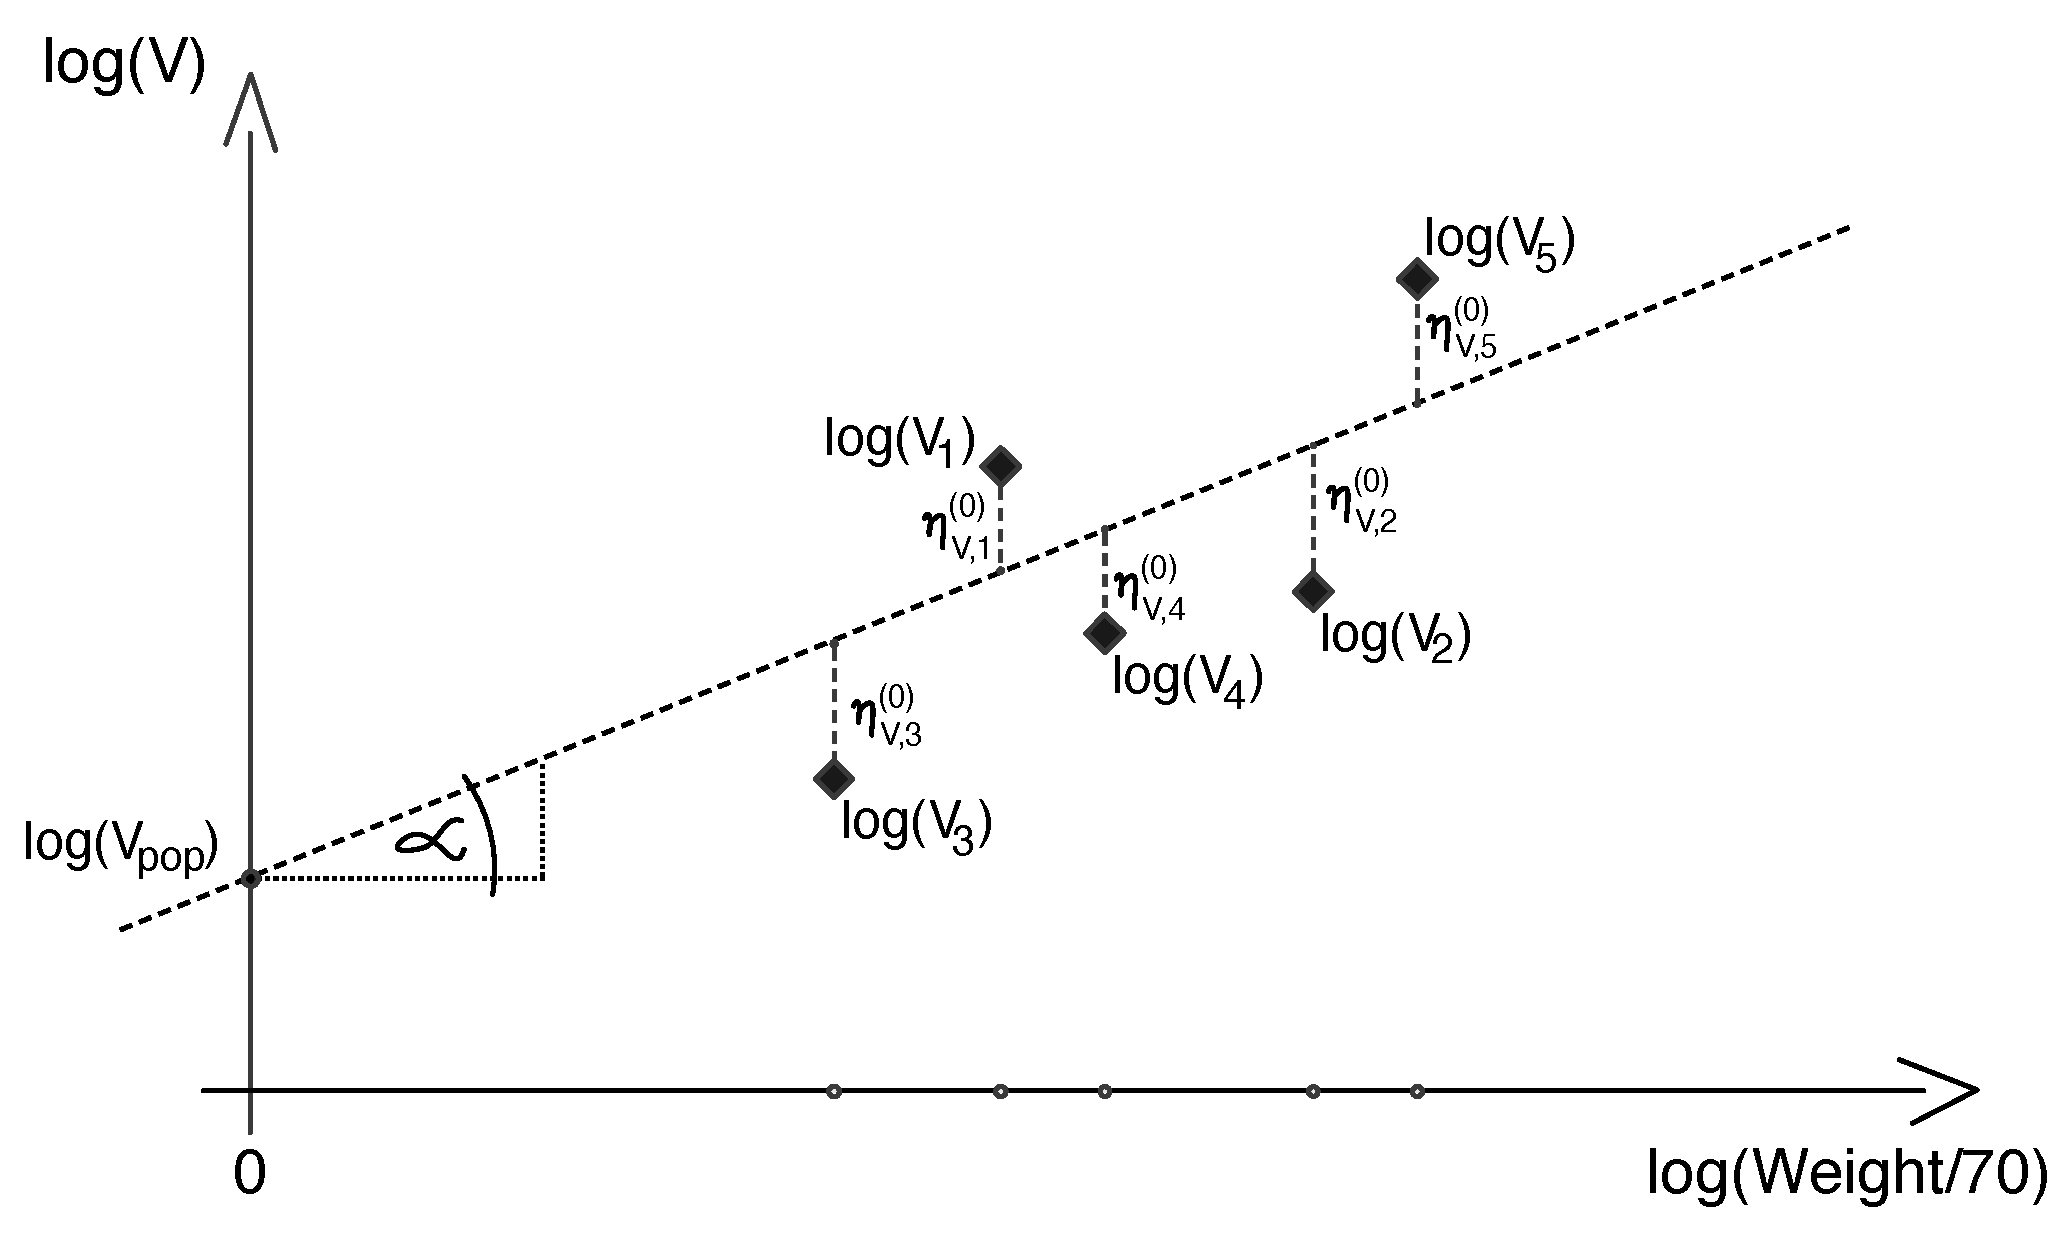
\includegraphics[width=100mm]{pics/weightAsCovariate.pdf}
\caption{The linear relationship between the parameter and a continuous covariate after application of appropriate transformations $V_i \longrightarrow \log(V_i)$ and $W \longrightarrow \log(W/70)$ with $\beta_{V,2} = \tan{\alpha}$, the slope of the regression line, and $\log(V_{pop})$ as the $y$-axis intercept.}
\label{fig:weightAsCovariate}
\end{figure}

%%%%%%%%%%%%%%%%%%%%%%%%%%%%%%%%%%%%%%%%%%%%%%%%%%%%%%%%%%%%%%%%%
\subsection{Correlation of random effects}\index{random effects!correlation structure}
\label{subsec:correlationModel}\label{maths:param correlation}
Correlation of random effects means that the transformed parameters. e.g. $\log(V_i)$ and $\log(CL_i)$ are correlated as well (although the relationship is not straightforward; see also the discussion below on correlation and covariates). There are two alternative ways to define the correlation, using either
\begin{itemize}
\item
a correlation matrix, $R$, or
\item
a variance-covariance matrix, $\Omega$.
\end{itemize}


\paragraph{Correlation matrix}\index{random effects!correlation matrix}
In this case it is sufficient to define the non-zero correlation coefficients, e.g. $\rho_{V,CL}$. All other off-diagonal correlation coefficients will be assumed to be equal to 0. For a simple one-compartment oral PK model with parameters $ka$, $V$, $CL$, and a correlation between $CL$ and $V$ the full correlation matrix reads as follows
\[
R =
 \begin{pmatrix}
  1 	& 0 	& 0  	\\
   		& 1	& \rho_{V,CL} \\
  		& 	& 1
 \end{pmatrix}
\]

\paragraph{Variance-covariance matrix}\index{random effects!variance-covariance matrix}
\label{maths:covariance-mat-derivation}
Alternatively, the variance-covariance matrix for the model
\[
 \Omega =
 \begin{pmatrix}
  \omega_{ka}^2 	& \omega_{ka,V}	& \omega_{ka,CL}\\
   			  	& \omega_{V}^2	& \omega_{V,CL} \\
  				& 				& \omega_{CL}^2
 \end{pmatrix}
 =
  \begin{pmatrix}
  \omega_{ka}^2 	& 0				& 0 \\
   			  	& \omega_{V}^2	& \omega_{V,CL} \\
  				& 				& \omega_{CL}^2
 \end{pmatrix}
\]
is providing the necessary information due to the reletionship
\begin{align*}
	&\mbox{Cov($p_i$,$p_j$)} = \sigma_i \sigma_j \mbox{Corr($p_i$,$p_j$)}  = \sigma_i \sigma_j \;\rho_{i,j} \quad \mbox{i.e.} \quad \omega_{V,CL} = \omega_V \omega_{CL} \rho_{V,CL}
\end{align*}
in which case it is enough to define $\Omega$ to cover the full correlation structure.

%%%%%%%%%%%%%%%%%%%%%%%%%%%%%%%%%%%%%%%%%%%%%%%%%%%%%%%%%%%%%%%%%
\subsection{Covariate model}\index{covariate model}
\label{maths:covariate_model}

The covariate model accounts for systematic or known subject
characteristics such as treatment group, gender or body
weight. Accordingly, the model can be defined for discrete and
continuous covariates and is the place where one category of fixed
effects is defined (the other being
the population averages, e.g. $V_{pop}$). Of course, the values of
individual characteristics (weight or sex) are subject specific but
the parameters assigned to them are identical for a group or
population.

As described in the example above the contribution of the continuous
covariate $Weight$ to the parameter value is formulated as
$\beta_{V,2} \log(W_i/70)$ (see figure
\ref{fig:weightAsCovariate}). The figure illustrates the linearity
after the appropriate transformation of the parameter, $V_i
\longrightarrow \log(V_i)$ and $W \longrightarrow \log(W/70)$ with
$\beta_{V,2} = \tan{\alpha}$, the slope of the regression line, and
$\log(V_{pop})$ as the $y$-axis intercept.

In the estimation case the values for the covariate are provided for
each individual. In the case of a simulation (see example
\ref{subsec:exp2_TaskDescription}) its probability distribution has to
be estimated. The information we have to provide is summarised in the
following
\paragraph{Continuous covariate model}\index{covariate model!continuous covariates}
\begin{align*}
Covariates & =  Weight  \\
CovariatesType & = Continuous  \\
CovariatesPopDistribution\{1\} & \sim \mbox{Normal}(pop_{Weight}, \omega_{Weight})  \\
 \text{with} & \quad pop_{Weight}=70.07 \\
 & \quad \omega_{Weight}=14.09  \\
CovariatesTransf & =\log(Weight/70) 
\end{align*}
Analog information has to be provided in the case of a categorical covariate, 
such as \textit{Sex} and is summarised for a simple example in the following

\paragraph{Categorial covariate model}\index{covariate model!categorical covariates}
\begin{align*}
Covariates &= Sex   \\
CovariatesType &= Categorical  \\
CategoriesNumber &= 2   \\
Categories &= \{F,M\}   \\
RefCategory &= F   \\
RefCategProbability &= 14/36 
\end{align*}


%%%%%%%%%%%%%%%%%%%%%%%%%%%%%%%%%%%%%%%%%%%%%%%%%%%%%%%%%%%%%%%%%%%
%%\subsection{Note on correlation and covariates}
%%This section discusses the influence of covariates on correlation between random effects and that of the parameters. In the case without e.g. normally distributed covariates, the correlation is identical. However, the presence of normally distributed body weight in the parameter model has interesting consequences for these correlations. \\
%%Let's consider as an example two correlated log-normally distributed parameters, $V$ and $CL$, without covariates i.e.
%%\begin{align*}
%%& \eta_{V} \sim \mathcal{N}(0,\omega_V); \quad \log( V ) = \log( V_{pop} ) + \eta_{V}  \\
%%& \eta_{CL} \sim \mathcal{N}(0,\omega_{CL}); \quad \log( CL ) = \log( CL_{pop} ) + \eta_{CL}
%%\end{align*}
%%then the correlation between the random effects is identical to the correlation of the (transformed) parameters, see Figure \ref{fig:correlationEtasLogedParams1}.
%%\begin{figure}[h!]
%%\centering
%% 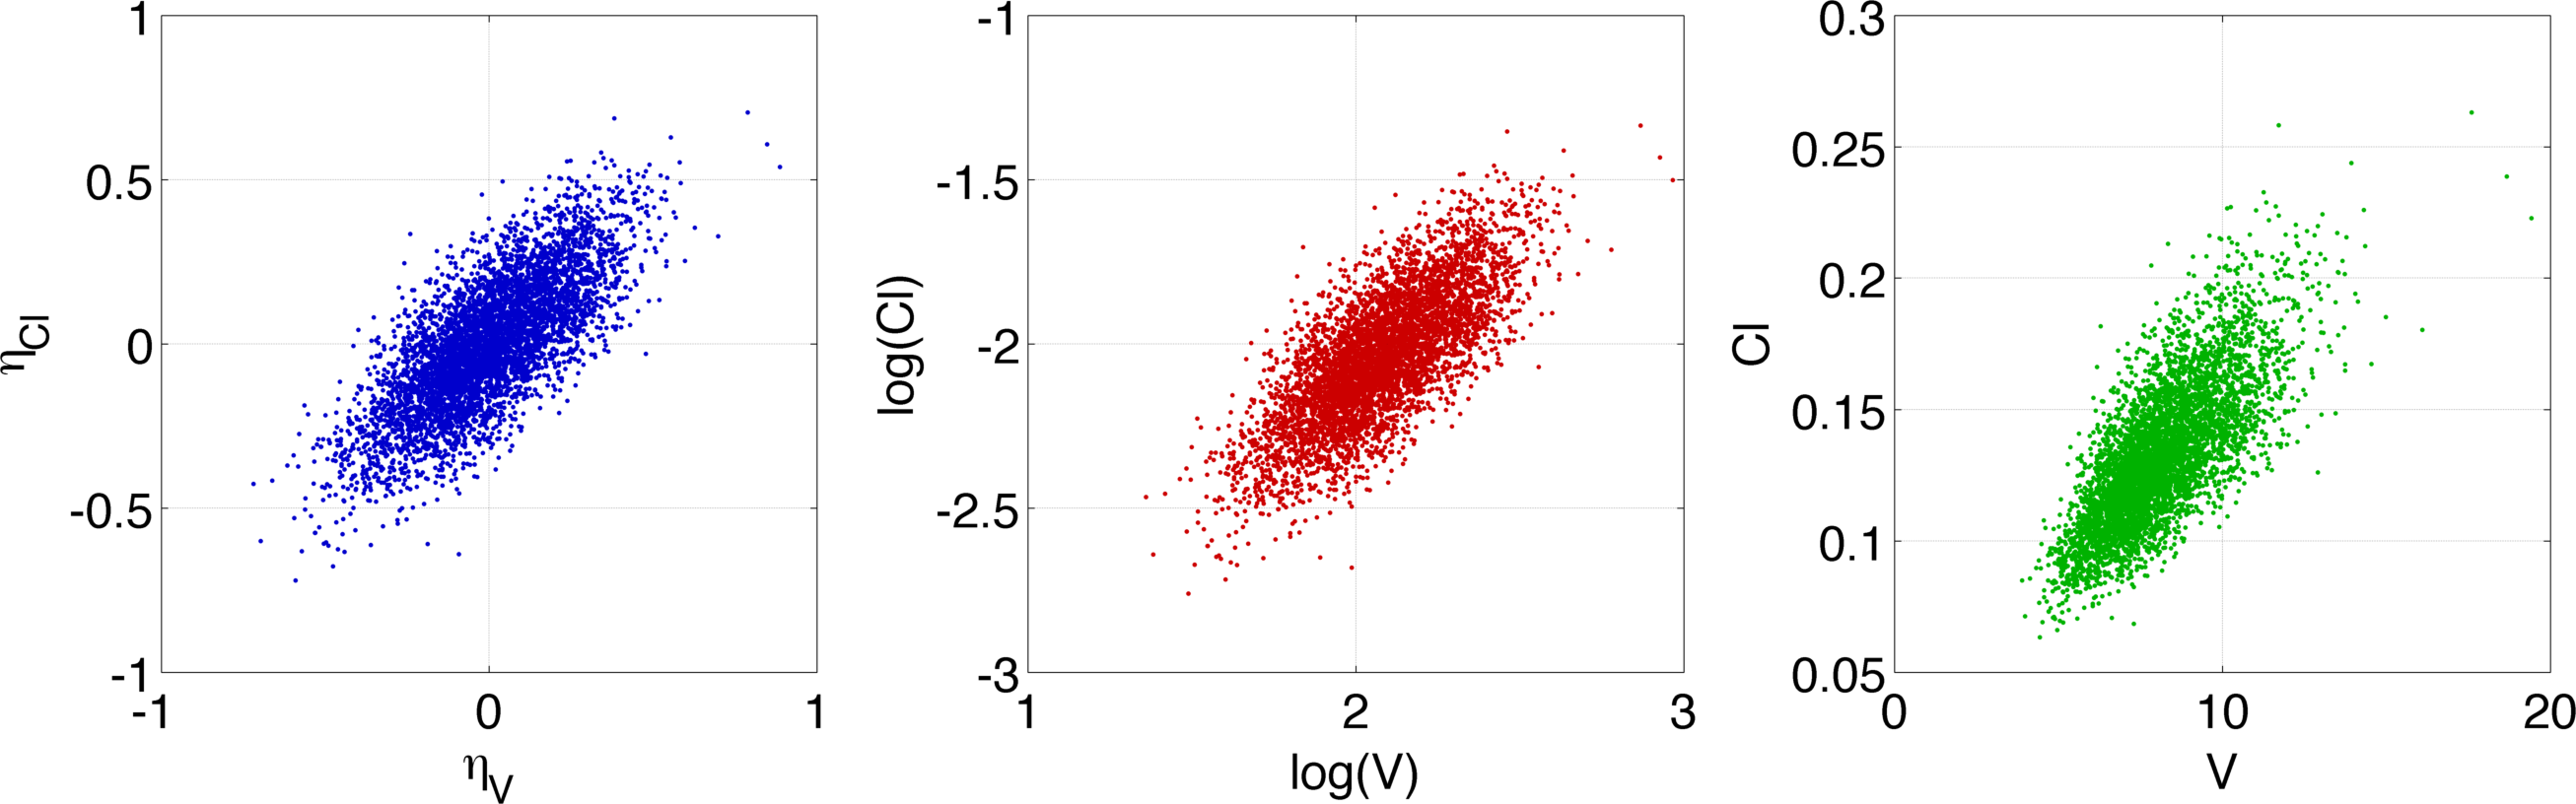
\includegraphics[height=45mm]{correlationsNoCovars}
%%\caption{Correlation of random effects $\eta_V$, $\eta_{CL}$ (blue), transformed parameters $\log(V)$ and $\log(CL)$ (red) and actual parameters  $V$ and $CL$ (green) is equal in the case without covariates. Values used: $V_{pop}=8, \omega_V=0.2, CL_{pop}=0.13,  \omega_{CL}=0.2$.}
%%\label{fig:correlationEtasLogedParams1}
%%\end{figure}
%%\newline
%%Now, we consider that both parameters depend on a continuous normally distributed covariate, e.g. the $Weight$,
%%\begin{align*}
%%& \eta_{V} \sim \mathcal{N}(0,\omega_V); \quad \log( V ) = \log( V_{pop} ) + \beta_{V} \log\Big(\frac{W}{70}\Big) + \eta_{V}  \\
%%& \eta_{CL} \sim \mathcal{N}(0,\omega_{CL}); \quad \log( CL ) = \log( CL_{pop} ) + \beta_{CL} \log\Big(\frac{W}{70}\Big) + \eta_{CL}
%%\end{align*}
%%then the correlation between the transformed parameters is higher then that of the random effects and increases proportionally to $corr(\eta_{V}, \eta_{CL})$, see Figure \ref{fig:correlationEtasLogedParams2}.
%%\begin{figure}[h!]
%%\centering
%% 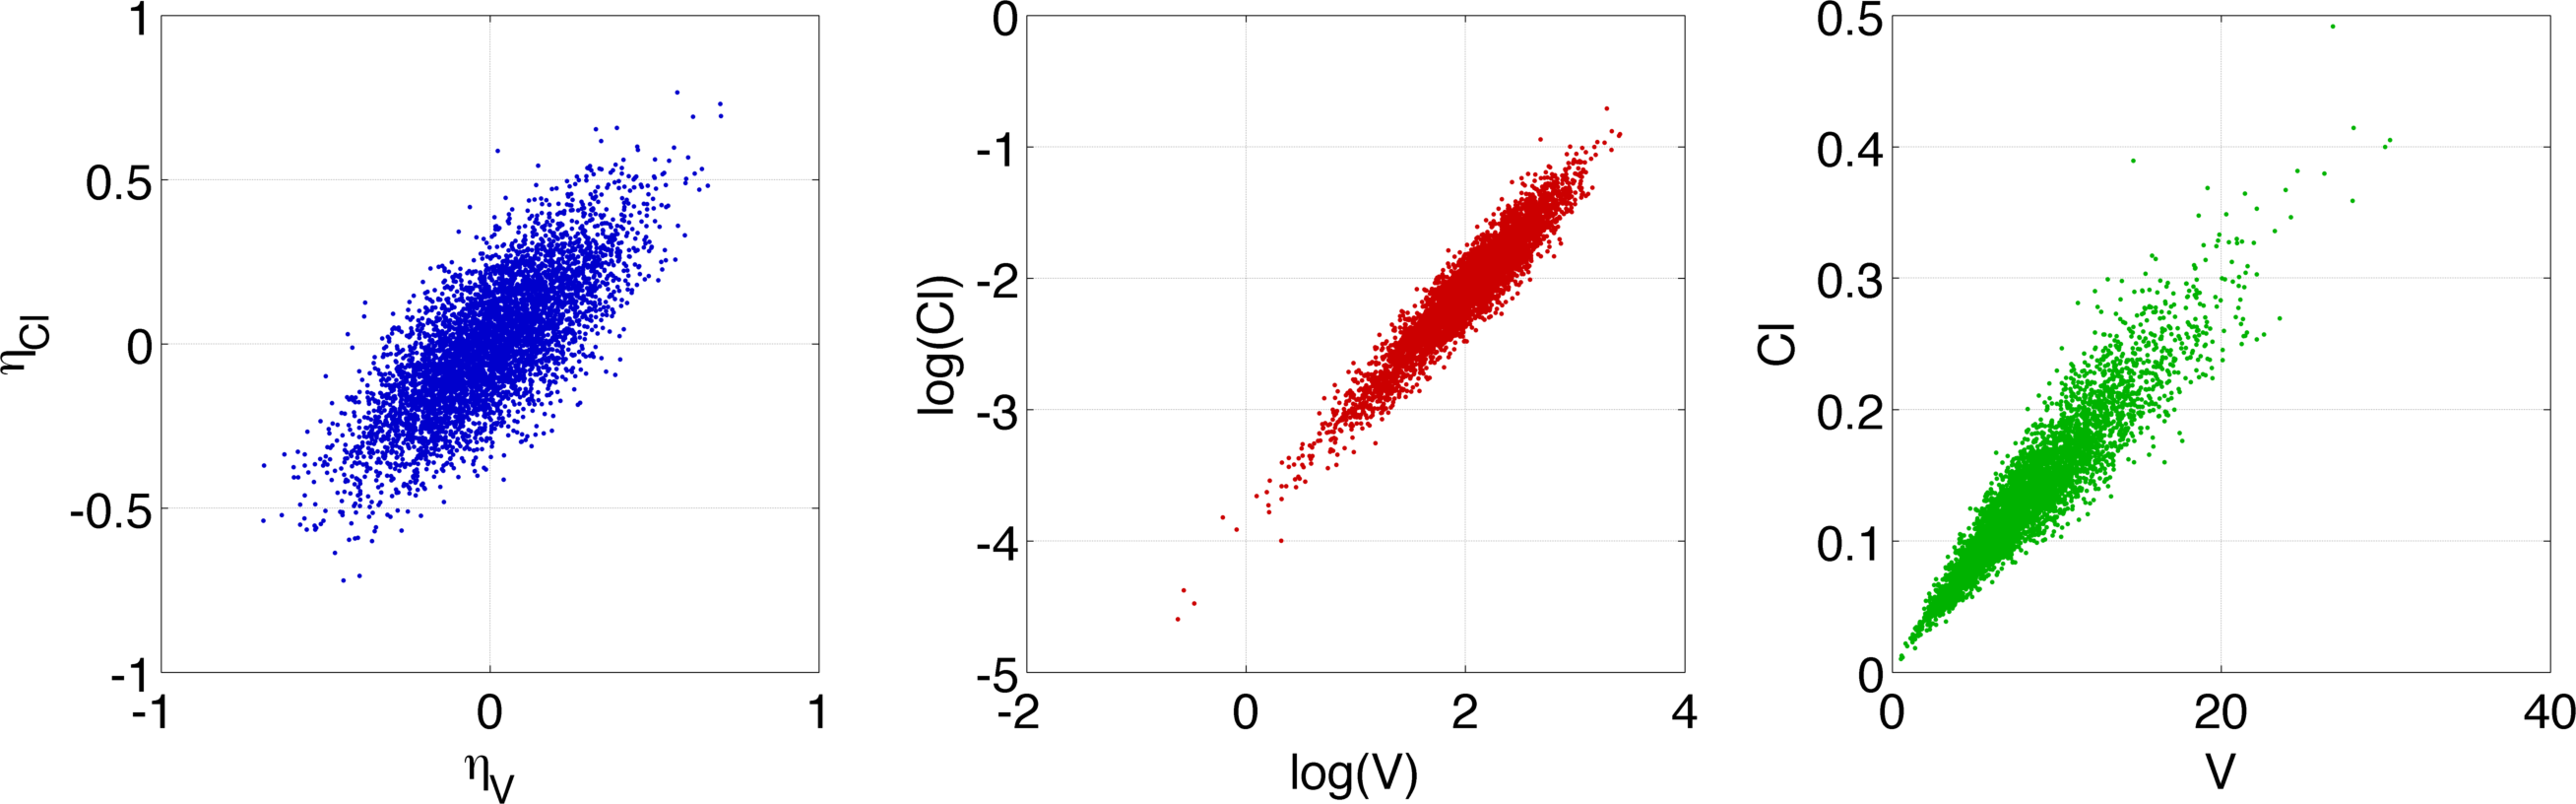
\includegraphics[height=45mm]{correlationsWithCovars}
%%\caption{The correlation between both the transformed parameters (red) and actual parameters (green) is higher then that of the random effects (blue) (and is equal 0.933, 0.948 and 0.750, respectively, for $n=10^8$). Values used as before with $\beta_V=2, \beta_{CL}= 1.75$.}
%%\label{fig:correlationEtasLogedParams2}
%%\end{figure}
%%\newline
%%The consequence of this discussion is that the correlation structure of random effects, as defined in PharmML, translates only in special cases to the correlation between parameters.
%%%This underlines the importance of the fact that we define in PharmML the relationship between random effects and not parameters.


%%%%%%%%%%%%%%%%%%%%%%%%%%%%%%%%%%%%%%%%%%%%%%%%%%%%%%%%%%%%%%%%%
\subsection{Equivalent representations of the parameter model}
Every parameter model represented in the Type 3 format discussed before has at least three mathematically equivalent representation forms,
which will be presented and discussed in terms of advantages and disadvantages in the following. It is important to understand these different
representation forms, as they explain the different forms of notation used in different software tools. Here, we concentrate on NONMEM and MONOLIX only.

%%%%%%%%%%%%%%%%%%%%%%%%%%%%%%%%%%%%%%%%%%%%%%%%%%%%%%%%%%%%%%%%%
% Log-Normal distributed
%%%%%%%%%%%%%%%%%%%%%%%%%%%%%%%%%%%%%%%%%%%%%%%%%%%%%%%%%%%%%%%%%

\subsubsection{Log-Normal distributed}
For a \textbf{log-normal} distributed parameter, e.g. $V$, the equivalent representations read
\begin{align*}
&(1) \eta_{i,V} \sim \mathcal{N}(0,\omega_V); \quad V_i= V_{pop} \; e^{\eta_{i,V}}   \\
&(2) \eta_{i,V} \sim \mathcal{N}(0,\omega_V); \quad \log( V_i ) = \log( V_{pop} ) + \eta_{i,V}  \\
&(3) \log( V_i ) \sim \mathcal{N}\big( \log( V_{pop} ),\omega_V\big)
\end{align*}
for a typical value $V_{pop}$ and standard deviation $\omega_V$ as described in \cite{LavielleBook:2014}.\\
The typical NMTRAN code for a log-normally distributed parameter is (\cite{Smith:2012aa})
\begin{lstlisting}
	GRPV=THETA(1)
	V=GRPV*EXP(ETA(1))
\end{lstlisting}
and in MLXTRAN (\cite{MonolixOverview:2012})
\begin{lstlisting}
	# as explicit equation
	eta_V ~ normal(0, omega_V)
	V = V_pop*exp(eta_V)

	# or using short notation
	V = {distribution=lognormal, typical=V_pop, sd=omega_V}
\end{lstlisting}

\begin{figure}[htbp]
\centering
 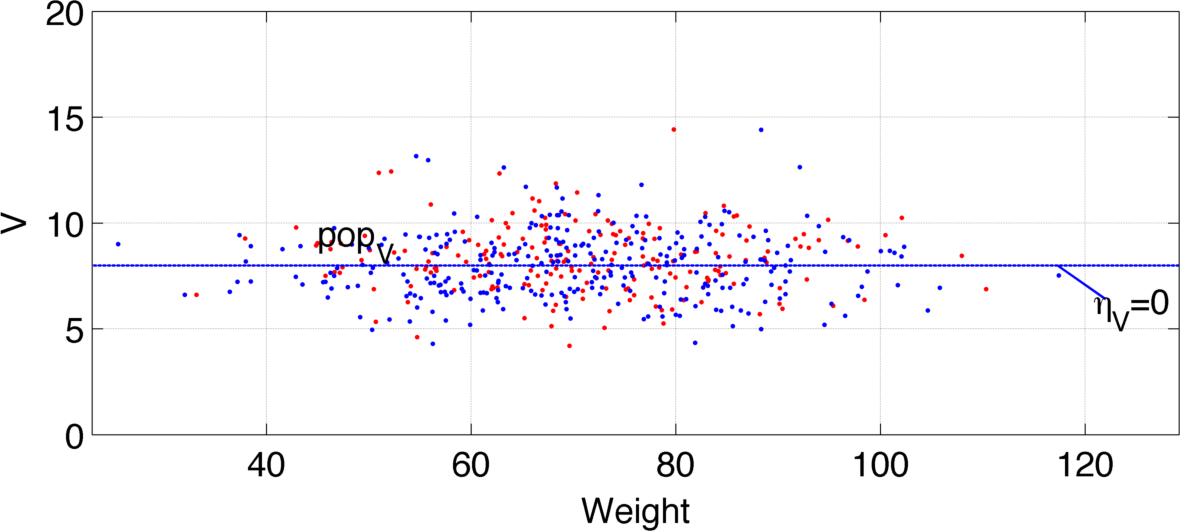
\includegraphics[width=100mm]{pics/paramCovModel_V}
\caption{Log-normally distributed 'V' with $V_{pop}=8$ and $\omega_V=0.2$}
\label{fig:parameterCovModel0}
\end{figure}


%%%%%%%%%%%%%%%%%%%%%%%%%%%%%%%%%%%%%%%%%%%%%%%%%%%%%%%%%%%%%%%%%
% Log-Normal distributed with a continuous covariate
%%%%%%%%%%%%%%%%%%%%%%%%%%%%%%%%%%%%%%%%%%%%%%%%%%%%%%%%%%%%%%%%%

\subsubsection{Log-Normal distributed with a continuous covariate}
For a \textbf{log-normal} distributed parameter, e.g. $V$, with body weight, $W$, as covariate the equivalent representations read
\begin{align*}
& (1) \quad \eta_{i,V} \sim \mathcal{N}(0,\omega_V); \quad V_i= V_{pop} \; \big(\frac{W_i}{70}\big)^\beta \; e^{\eta_{i,V}}   \\
&(2) \quad \eta_{i,V} \sim \mathcal{N}(0,\omega_V); \quad \log( V_i ) = \log( V_{pop} ) + \beta \log\big(\frac{W_i}{70}\big) + \eta_{i,V}  \\
&(3) \quad \log( V_i ) \sim \mathcal{N}\big( \log( V_{pop} )+ \beta\log\Big(\frac{W_i}{70}\Big),\omega_V\big)
\end{align*}
The typical NMTRAN code for a log-normally distributed parameter with weight as covariate is
\begin{lstlisting}
	GRPV=THETA(1)*(WT/70)**THETA(2)
	V=GRPV*EXP(ETA(1))
\end{lstlisting}
and in MLXTRAN
\begin{lstlisting}
	# as explicit equation
	V_pop = V_pop*(weight/70)^beta_V
	eta_V ~ normal(0, omega_V)	
	V = V_pop*exp(eta_V)

	# or using short notation
	V = {distribution=lognormal, typical=V_pop, covariate=lw70, coefficient=beta_V, sd=omega_V}
\end{lstlisting}
with $lw70 \equiv \log(W/70)$.

\begin{figure}[htbp]
\centering
 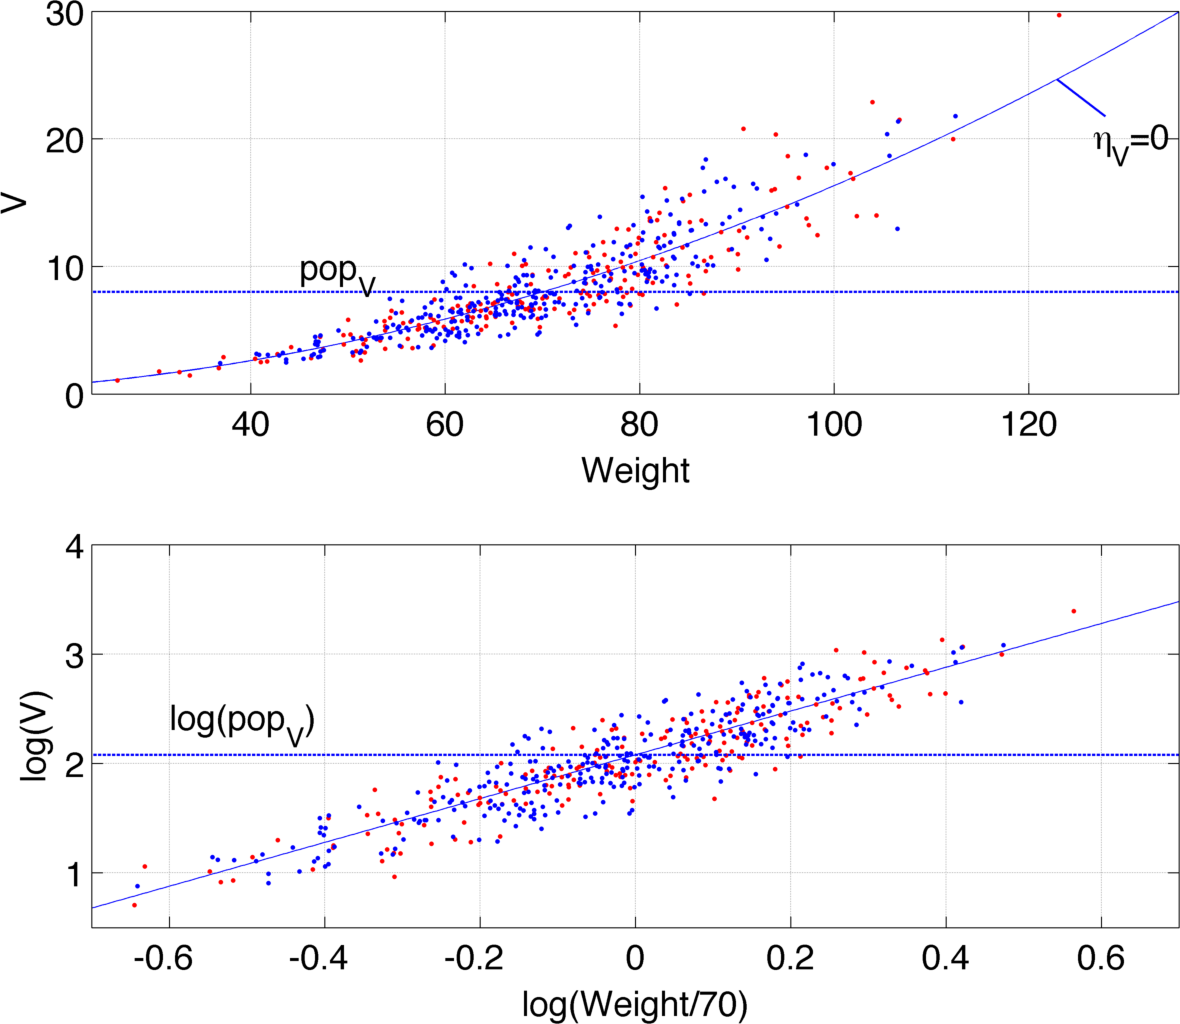
\includegraphics[width=100mm]{pics/paramCovModel_VlogV}
\caption{Log-normally distributed 'V' with 'Weight' as covariates.}
\label{fig:parameterCovModel1}
\end{figure}


%%%%%%%%%%%%%%%%%%%%%%%%%%%%%%%%%%%%%%%%%%%%%%%%%%%%%%%%%%%%%%%%%
% Logit-Normal distributed
%%%%%%%%%%%%%%%%%%%%%%%%%%%%%%%%%%%%%%%%%%%%%%%%%%%%%%%%%%%%%%%%%

\subsubsection{Logit-Normal distributed}
For a \textbf{logit-normal} distributed parameter, e.g. $Imax$, the equivalent representations read
\begin{align*}
&(1) \quad \eta_{i,Imax} \sim \mathcal{N}(0,\omega); \quad  Imax_i= \frac{\bigg[\frac{ Imax_{pop}}{1- Imax_{pop}} \; e^{\eta_{i, Imax}} \bigg]}{ 1+  \bigg[\frac{ Imax_{pop}}{1- Imax_{pop}} \; e^{\eta_{i, Imax}} \bigg]}   \\
&(2) \quad  \eta_{i,Imax} \sim \mathcal{N}(0,\omega); \quad \mbox{logit}(  Imax_i ) = \mbox{logit}(  Imax_{pop} ) + \eta_{i, Imax}  \\
&(3) \quad  \mbox{logit}(  Imax_i ) \sim \mathcal{N}\big( \mbox{logit}( Imax_{pop} ),\omega\big)
\end{align*}
Equation (1) can be rewritten using '$logit$' as follows
\begin{align*}
& Imax_i= \frac{\exp\big(logit(Imax_{pop})  + \eta_{i,Imax} \big)}{ 1+ \exp\big(logit(Imax_{pop}) + \eta_{i,Imax} \big)}  \\
& \Leftrightarrow  Imax_i= \frac{1}{ 1+ \exp\big(- logit(Imax_{pop}) - \eta_{i,Imax} \big)}
\end{align*}\newline
The last form is used for a typical NMTRAN implementation of a logit-normally distributed parameter
\begin{lstlisting}
	LGTIMAX=LOG(POP_IMAX/(1-POP_IMAX)) + ETA(IMAX)
	IMAX=1/(1+EXP(-LGTIMAX))
\end{lstlisting}
and in MLXTRAN
\begin{lstlisting}
	# as explicit equation
	eta_Imax ~ normal(0, omega_Imax)
	logitImaxi = log(pop_Imax/(1-pop_Imax)) + eta_Imax
	Imaxi = 1/(1 + exp(-logitImaxi))

	# or using short notation
	Imax = {distribution=logitnormal, typical=Imax_pop, sd=omega_Imax}
\end{lstlisting}


%%%%%%%%%%%%%%%%%%%%%%%%%%%%%%%%%%%%%%%%%%%%%%%%%%%%%%%%%%%%%%%%%
% Logit-Normal distributed with a continuous covariate
%%%%%%%%%%%%%%%%%%%%%%%%%%%%%%%%%%%%%%%%%%%%%%%%%%%%%%%%%%%%%%%%%

\subsubsection{Logit-Normal distributed with a continuous covariate}
For a \textbf{logit-normal} distributed parameter with \textit{Weight} as \textbf{covariate} we have
\begin{align*}
&(1)\quad \eta_{i,Imax} \sim \mathcal{N}(0,\omega); \quad Imax_i= \frac{\bigg[\frac{Imax_{pop}}{1-Imax_{pop}} \; \big(\frac{W_i}{70}\big)^\beta \; e^{\eta_{i,Imax}} \bigg]}{ 1+  \bigg[\frac{Imax_{pop}}{1-Imax_{pop}} \; \big(\frac{W_i}{70}\big)^\beta \; e^{\eta_{i,Imax}} \bigg]}
\end{align*}
\begin{align*}
&(2)\quad \eta_{i,Imax} \sim \mathcal{N}(0,\omega); \quad \mbox{logit}( Imax_i ) = \mbox{logit}( Imax_{pop} ) + \beta \log\bigg(\frac{W_i}{70}\bigg) + \eta_{i,Imax}  \\
&(3)\quad \mbox{logit}(  Imax_i ) \sim \mathcal{N}\big( \mbox{logit}( Imax_{pop}) + \beta\log\Big(\frac{W_i}{70}\Big),\omega\big)
\end{align*}
The first equation can be rewritten as follows
\begin{align*}
& Imax_i= \frac{\exp\big(logit(Imax_{pop}) + \beta \log\big(\frac{W_i}{70}\big) + \eta_{i,Imax} \big)}{ 1+ \exp\big(logit(Imax_{pop}) + \beta \log\big(\frac{W_i}{70}\big) + \eta_{i,Imax} \big)}  \\
& \Leftrightarrow Imax_i= \frac{1}{ 1+ \exp\big(- logit(Imax_{pop}) - \beta \log\big(\frac{W_i}{70}\big) - \eta_{i,Imax} \big)}
\end{align*}\newline
The last form is used for a typical NMTRAN implementation of a logit-normally distributed parameter with covariate
\begin{lstlisting}
	LGTIMAX=LOG(POP_IMAX/(1-POP_IMAX)) + BETA*LOG(WT/70) + ETA(IMAX)
	IMAX=1/(1+EXP(-LGTIMAX))
\end{lstlisting}
and in MLXTRAN
\begin{lstlisting}
	# as explicit equation
	eta_Imax ~ normal(0, omega_Imax)
	logitImaxi = log(pop_Imax/(1-pop_Imax)) + beta*lw70 + eta_Imax
	Imaxi = 1/(1 + exp(-logitImaxi))

	# or using short notation
	Imax =	{distribution=lognormal, typical=Imax_pop, covariate=lw70, coefficient=beta_Imax, sd=omega_Imax}
\end{lstlisting}

\begin{figure}[htbp]
\centering
 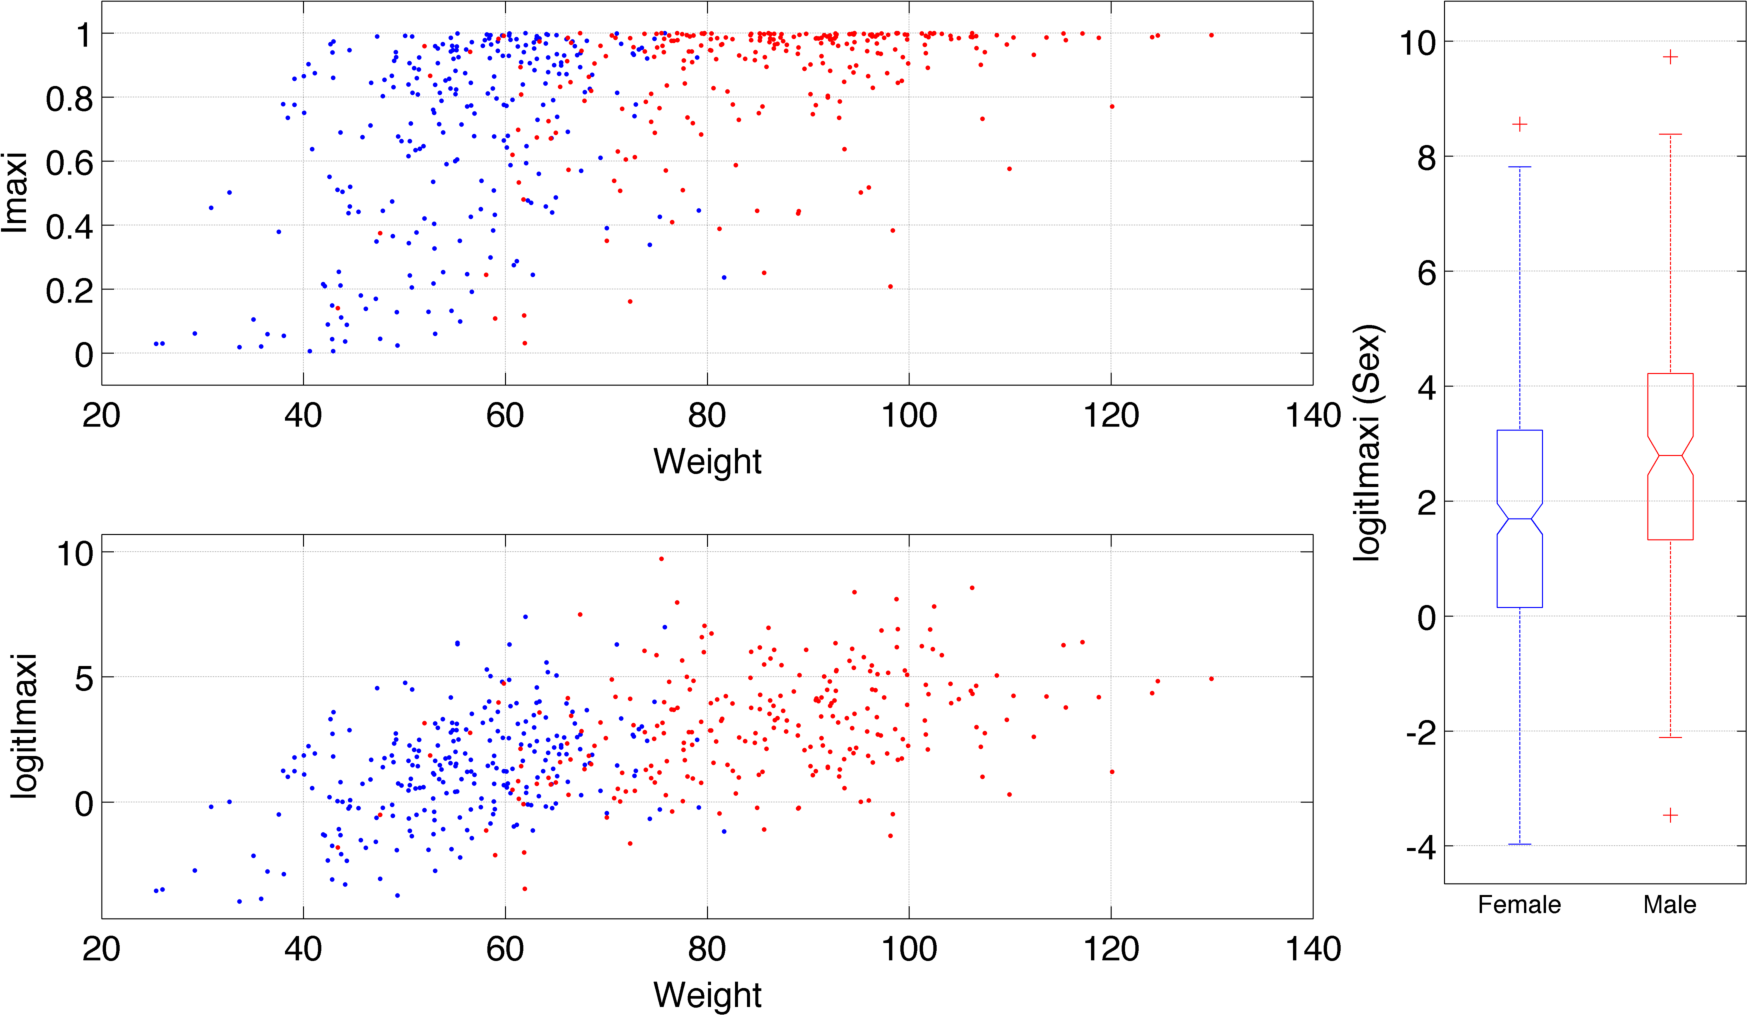
\includegraphics[width=100mm]{pics/paramCovModel_ImaxlogImax_Weight}
\caption{Logit-normally distributed 'Imax' with 'Weight' as covariate.}
\label{fig:parameterCovModel3}
\end{figure}


%%%%%%%%%%%%%%%%%%%%%%%%%%%%%%%%%%%%%%%%%%%%%%%%%%%%%%%%%%%%%%%%%%
%% Logit-Normal distributed with a categorical covariate
%%%%%%%%%%%%%%%%%%%%%%%%%%%%%%%%%%%%%%%%%%%%%%%%%%%%%%%%%%%%%%%%%%
%
%\subsubsection{Logit-Normal distributed with a categorical covariate}
%For a \textbf{logit-normal} distributed parameter with \textit{Sex} as \textbf{covariate} we have
%\begin{align*}
%&(1)\quad \eta_i \sim \mathcal{N}(0,\omega); \quad Imax_i= \frac{\bigg[\frac{Imax_{pop}}{1-Imax_{pop}} \; e^{\beta_{Imax_i} 1_{Sex_i=F}} \; e^{\eta_{i,Imax}} \bigg]}{ 1+  \bigg[\frac{Imax_{pop}}{1-Imax_{pop}} \; e^{\beta_{Imax_i} 1_{Sex_i=F}} \; e^{\eta_{i,Imax}} \bigg]}  \\
%&(2)\quad \eta_i \sim \mathcal{N}(0,\omega); \quad \mbox{logit}( Imax_i ) = \mbox{logit}( Imax_{pop} ) + \beta_{Imax_i} 1_{Sex_i=F} + \eta_{i,Imax}  \\
%&(3)\quad \mbox{logit}(  Imax_i ) \sim \mathcal{N}\big( \mbox{logit}( Imax_{pop}) + \beta_{Imax_i} 1_{Sex_i=F},\omega\big)
%\end{align*}
%The first equation can be rewritten as follows
%\begin{align*}
%& Imax_i= \frac{\exp\big(logit(Imax_{pop}) + \beta_{Imax_i} 1_{Sex_i=F} + \eta_{i,Imax} \big)}{ 1+ \exp\big(logit(Imax_{pop}) + \beta_{Imax_i} 1_{Sex_i=F} + \eta_{i,Imax} \big)}  \\
%& \Leftrightarrow Imax_i= \frac{1}{ 1+ \exp\big(- logit(Imax_{pop}) - \beta_{Imax_i} 1_{Sex_i=F} - \eta_{i,Imax} \big)}
%\end{align*}\newline
%The last form is used for a typical implementation of a logit-normally distributed parameter with covariate:\\
%in NMTRAN
%\begin{lstlisting}
%LGTIMAX=LOG(POP_IMAX/(1-POP_IMAX)) + BETA*SEX + ETA(IMAX)
%IMAX=1/(1+EXP(-LGTIMAX))
%\end{lstlisting}
%and in MLXTRAN
%\begin{lstlisting}
%# as explicit equation
%eta_Imax ~ normal(0, omega_Imax)
%logitImaxi = log(pop_Imax/(1-pop_Imax)) + beta*Sex + eta_Imax
%Imaxi = 1/(1 + exp(-logitImaxi))
%
%# or using short notation
%Imax =	{distribution=lognormal, typical=Imax_pop, covariate=Sex, coefficient=beta_Imax, sd=omega_Imax}
%\end{lstlisting}
%
%
%\begin{figure}[h!]
%\centering
% 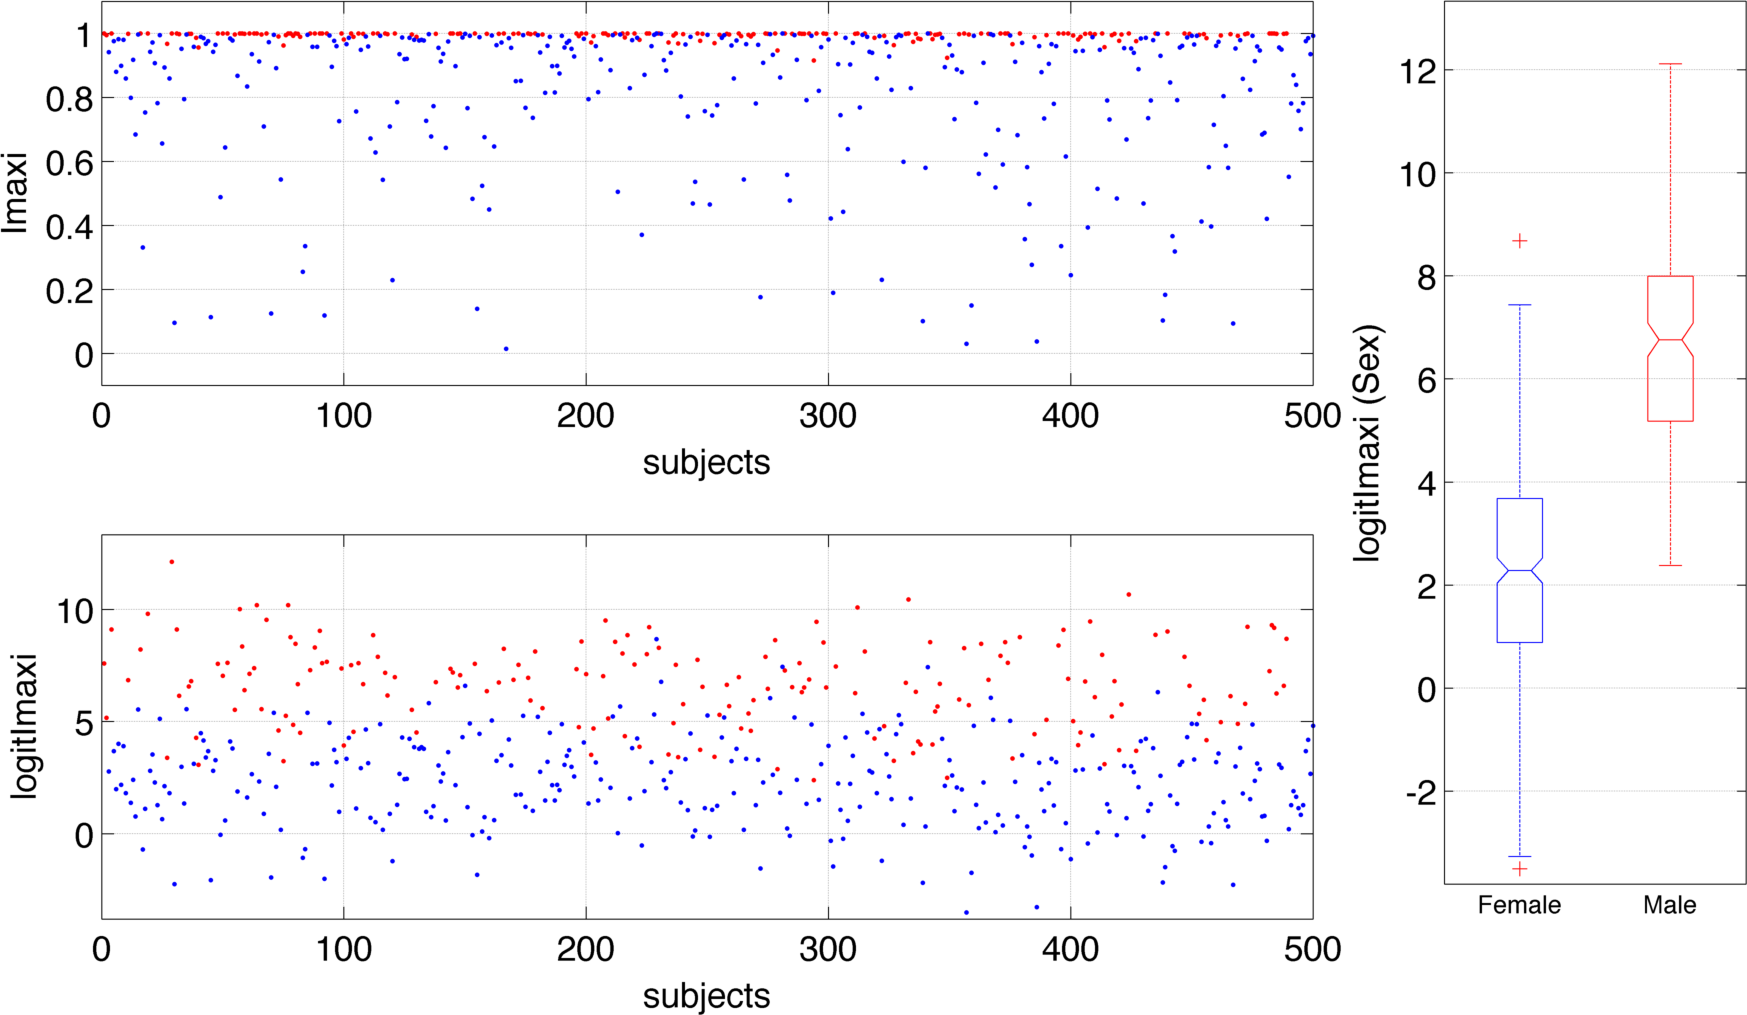
\includegraphics[width=100mm]{paramCovModel_ImaxlogImax_Sex}
%\caption{Logit-normally distributed 'Imax' with 'Sex' as a categorical covariate.}
%\label{fig:parameterCovModel4}
%\end{figure}


%%%%%%%%%%%%%%%%%%%%%%%%%%%%%%%%%%%%%%%%%%%%%%%%%%%%%%%%%%%%%%%%%
% Log-Normal distributed with complex variability structure
%%%%%%%%%%%%%%%%%%%%%%%%%%%%%%%%%%%%%%%%%%%%%%%%%%%%%%%%%%%%%%%%%

\subsubsection{Log-Normal distributed with complex variability structure}
\label{subsec:logIOVCovariate}
In this example we consider representations of type (1) and (2) only. A typical parameter model with a continuous covariate, $W$, for three levels of variability e.g. \{centre, subject, occasion\} (this will be explained in detail in next section), see Figure \ref{tree_IOV1}, reads as follows
\begin{align*}
&(1)\quad V_{lik} = V_{pop} \; \big(\frac{W_i}{70}\big)^\beta \; e^{\eta_{l,V}^{(-1)}} \; e^{\eta_{li,V}^{(0)}} \; e^{\eta_{lik,V}^{(+1)}}   \\
&(2)\quad \log(V_{lik}) = \log(V_{pop}) + \beta\log\Big(\frac{W_i}{70}\Big) + \eta_{l,V}^{(-1)} + \eta_{li,V}^{(0)} + \eta_{lik,V}^{(+1)}
\end{align*}
with
\begin{align*}
 & \eta_l^{(-1)} \sim \mathcal{N}\big(0,\Omega^{(-1)}\big), \quad \eta_{li}^{(0)} \sim \mathcal{N}\big(0,\Omega^{(0)}\big),
\quad \eta_{lik}^{(+1)} \sim \mathcal{N}\big(0,\Omega^{(+1)}\big)
\end{align*}
with $l$ -- centre index, $i$ -- subject index, $k$ -- occasion index.


%%%%%%%%%%%%%%%%%%%%%%%%%%%%%%%%%%%%%%%%%%%%%%%%%%%%%%%%%%%%%%%%%
% Discussion
%%%%%%%%%%%%%%%%%%%%%%%%%%%%%%%%%%%%%%%%%%%%%%%%%%%%%%%%%%%%%%%%%
%
%\subsection{Discussion}
%Currently, \pharmml supports the version (2) of the parameter model. Consider the parameter model from last example
%which with some additional annotation reads as follows
%\begin{align*}
%& \underbrace{\log(V_{lik})}_{\text{\parbox{2cm}{\centering transformed\\[-4pt] individual value}}} = \underbrace{\log(V_{pop})}_{\text{\parbox{2cm}{\centering transformed\\[-4pt] typical value}}} + \underbrace{\beta\log\Big(\frac{W_i}{70}\Big)}_{\text{covariate model}}
%+ \underbrace{\eta_{l,V}^{(1)}}_{\text{\parbox{2cm}{\centering inter-centre\\[-4pt]  variability}}}
%+ \underbrace{\eta_{li,V}^{(0)}}_{\text{\parbox{2cm}{\centering inter-individual\\[-4pt] within centre \\[-4pt]  variability}}}
%+ \underbrace{\eta_{lik,V}^{(-1)}}_{\text{\parbox{2.5cm}{\centering inter-occasion\\[-4pt] within individual \\[-4pt] within centre \\[-4pt] variability}}}
%\end{align*}
%This formula, linear for the transformed parameter, has the following \textbf{advantages}
%\begin{itemize}
%\item
%it has an additive structure allowing for easy interpretation and implementation of its components, i.e.
%\begin{itemize}
%\item
%typical/population value of the parameter
%\item
%covariate model
%\item
%any level of random effects
%\end{itemize}
%\item
%it covers the majority of models relevant for daily practice
%\end{itemize}
%The \textbf{disadvantage} is that it doesn't cover parameter models which cannot be represented in the linear form for the transformed parameter, e.g. the models proposed by \cite{Keizer:2011aa}. This issue has been recognised early on and discussed in the consortium. This class of models is being considered for a subsequent specification of \pharmml.


%
%\paragraph{Discussion}
%Consider for example equation (2) for a parameter with a continuous covariate, $W$, with three levels of variability e.g. \{country,subject, occasion\} from the last example. With some additional annotation it reads then
%\begin{align*}
%& \underbrace{\log(V_{lik})}_{\parbox{2cm}{\centering transformed\\[-4pt] individual\\[-4pt] value}} = \underbrace{\log(V_{pop})}_{\parbox{1.5cm}{\centering transformed\\[-4pt] typical\\[-4pt] value}}
%+ \underbrace{\beta\log\Big(\frac{W_i}{70}\Big)}_{\parbox{2cm}{\centering covariate\\[-4pt] model}}
%+ \underbrace{\eta_{l,V}^{(1)}}_{\parbox{2cm}{\centering inter-centre\\[-4pt]  variability}}
%+ \underbrace{\eta_{li,V}^{(0)}}_{\parbox{2.25cm}{\centering inter-centre-\\[-4pt] individual\\[-4pt]  variability}}
%+ \underbrace{\eta_{lik,V}^{(-1)}}_{\parbox{3cm}{\centering inter-centre-\\[-4pt] individual-occasion\\[-4pt] variability}}
%\end{align*}
%
%This formulation, linear for the transformed parameter, has the following advantages
%\begin{itemize}
%\item
%it has an additive structure allowing for easy interpretation and implementation of its components, i.e.
%\begin{itemize}
%\item
%typical/population value of the parameter
%\item
%covariate model
%\item
%inter-individual variability random effects
%\item
%higher levels of variability
%\end{itemize}
%\item
%it covers the majority of models relevant for daily practice
%\end{itemize}
%More complex models will be supported in an upcoming specification.
%


\section{Observation model}
\label{sec:observationModel}
Figure \ref{fig:observModel} shows the classification of continuous and discrete data models in \pml \currpml. 
The defining characteristic of data is their distribution which will be described first
\begin{itemize}
\item
Continuous data
\begin{itemize}
\item
usually described by the normal distribution.
\end{itemize}
\item
Discrete data
\begin{itemize}
\item
Count data -- non-negative integers -- described by the Poisson or a related distribution.
\item
Categorical data -- finite set of integer values, nominal or ordered -- described by the Bernoulli
or the categorical distribution. 
\item
Time-to-event data -- time until an event occurs, can be unique or repeated -- described by 
survival or hazard function.
\end{itemize}
\end{itemize}

\begin{figure}[h!]
\centering
 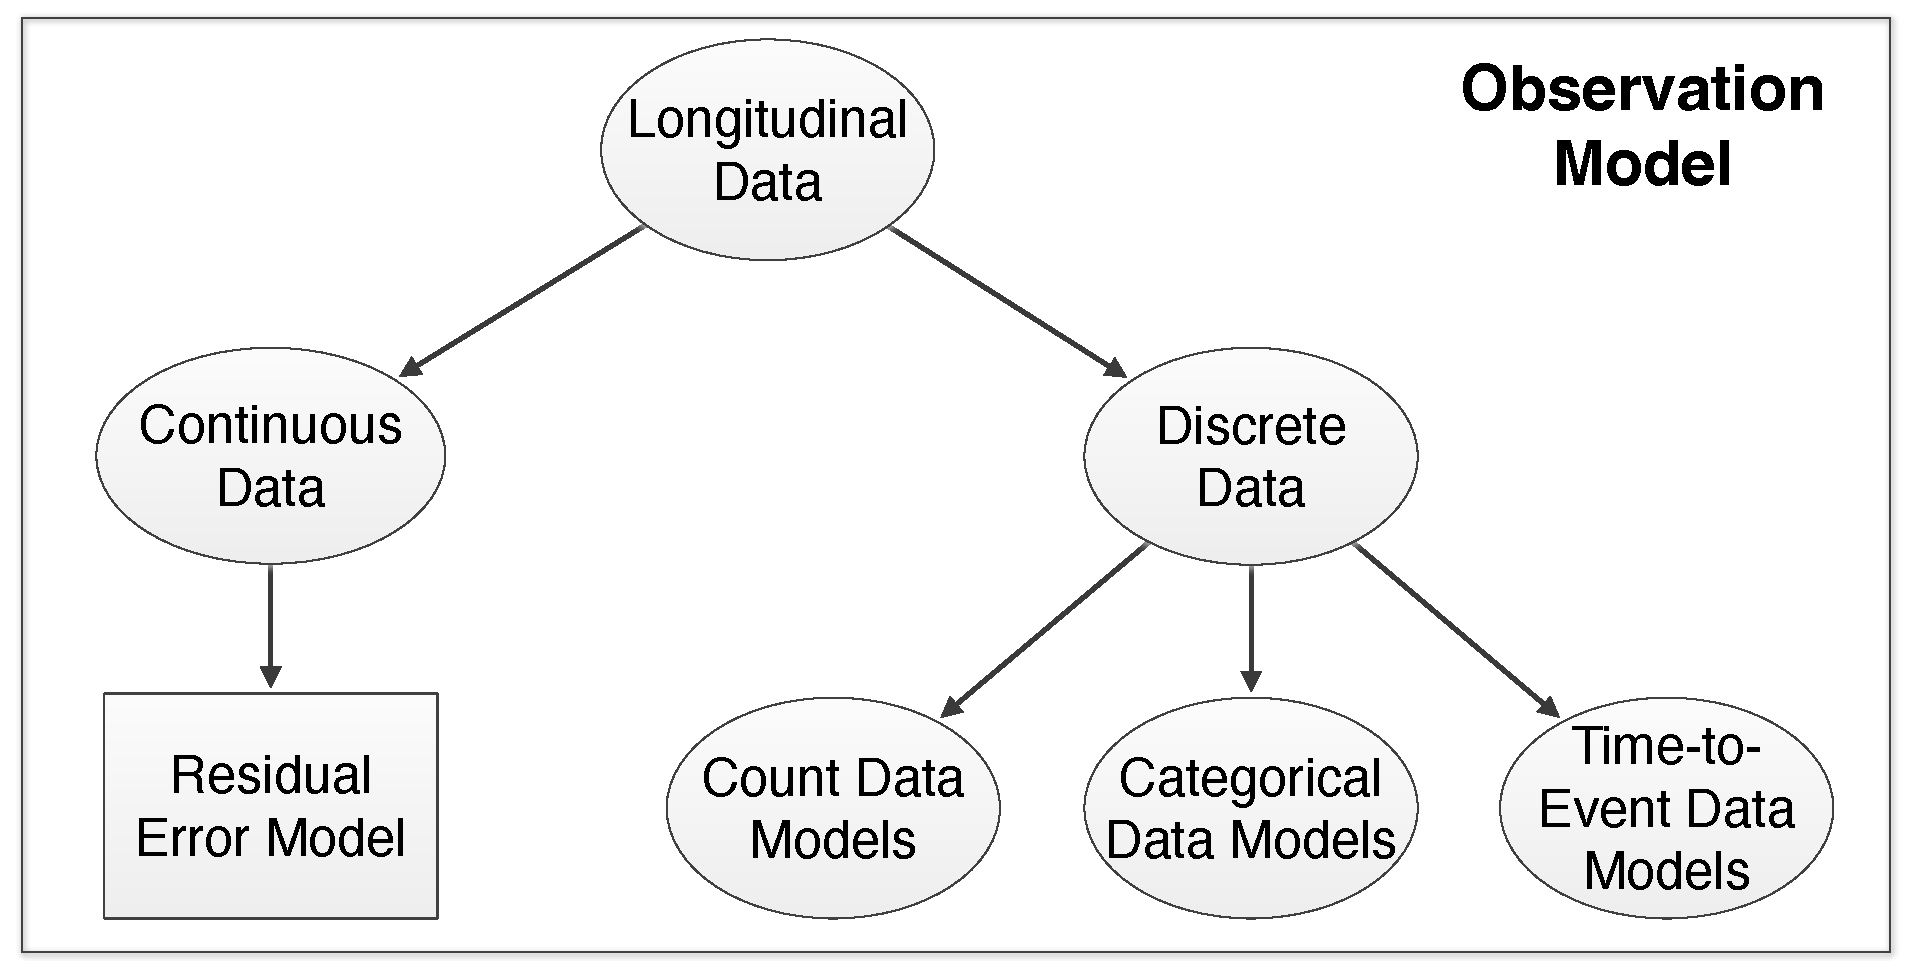
\includegraphics[height=75mm]{pics/observationalModel}
\caption{Observation model for continuous and discrete data. 
The residual error model of continuous data is described by a continuous distribution 
(e.g. normal distribution), while the error distribution of discrete data
is described by a discrete distribution (e.g. binomial for binary data).}
\label{fig:observModel}
\end{figure}


%%%%%%%%%%%%%%%%%%%%%%%%%%%%%%%%%%%%%%%%%%%%%%%%%%%%%%%%%%%%%%%%%%
\subsection{Contiuous data}
\label{subsec:ContinuesData}

An essential component of the continuous observation model is the residual error model.

%%%%%%%%%%%%%%%%%%%%%%%%%%%%%%%%%%%%%%%%%%%%%%%%%%%%%%%%%%%%%%%%%%
\subsubsection{Residual error model}
\label{sec:residualErrorModel}
\label{maths:error_model}
\label{maths:combined-err-model}
In this section we consider different forms of the residual error, i.e. this section is about $g$ in the term
\begin{align*}
g(x_{ij}, \psi_{i}, \xi) \epsilon_{ij}
\end{align*}
of eq.\ref{eq:nlmeModel} with $\epsilon_{ij} \sim N(0, 1)$, i.e. a standard normally distributed random variable. We distinguish between
\begin{itemize}\addtolength{\itemsep}{-.95\baselineskip}
\item
models for \textbf{untransformed} data
\begin{align*}
 \underbrace{ y_{ij}}_{\text{\parbox{2cm}{\centering Experimental \\[-4pt]  data}}} =
 \underbrace{ f(x_{ij}, \psi_{i})}_{\text{\parbox{2.5cm}{\centering Model \\[-4pt]  prediction}}} +
 \underbrace{ g(x_{ij}, \psi_{i}, \xi_i) \; \epsilon_{ij}}_{\text{\parbox{3cm}{\centering Residual \\[-4pt] error}}}
 \end{align*}
 \item
\textbf{transform-both-sides} models
\begin{eqnarray}
 \underbrace{ u(y_{ij})}_{\text{\parbox{2cm}{\centering Transformed \\[-4pt] experimental \\[-4pt]  data}}} =
 \underbrace{ u\big(f(x_{ij}, \psi_{i})\big)}_{\text{\parbox{2.5cm}{\centering Transformed \\[-4pt]  model \\[-4pt]  prediction}}} +
 \underbrace{ g(x_{ij}, \psi_{i}, \xi_i) \; \epsilon_{ij}}_{\text{\parbox{3cm}{\centering Residual \\[-4pt] error}}} \nonumber
 \end{eqnarray}
 \item
and \textbf{implicit} models
\begin{eqnarray}
 \underbrace{ u(y_{ij})}_{\text{\parbox{2.5cm}{\centering Transformed \\[-4pt] experimental  data}}} =
 \underbrace{ U\big(f(x_{ij}, \psi_{i}),\xi_i, \epsilon_{1,ij}, \epsilon_{2,ij}, \dots\big)}_{\text{\parbox{2.5cm}{\centering Transformed \\[-4pt]  model prediction}}} \nonumber
 \end{eqnarray}
\end{itemize}
The \textit{untransformed} form is a special case of the \textit{transform-both-sides} form with $u \equiv Id$, i.e. the identity transformation.
Then for models of both types with $\epsilon_{ij}$ being normally distributed with mean 0 and variance 1, $u(y_{ij})$ is also normally distributed
with mean $u(f(x_{ij}, \psi_{i}))$ and the standard deviation $g(x_{ij}, \psi_{i}, \xi_i)$. \\
Possible extensions to the basic models are
\begin{itemize}
\item
when more than one random variable is applied, i.e. multiple $\epsilon$'s,
\item
when more than one type of measurement or observation is defined, or
\item
when variability, as discussed in section \ref{sec:variabilityModel}, is applied to parameters of the residual error model (see section \ref{subsec:varModelResidualError} for details).
\end{itemize}


%%%%%%%%%%%%%%%%%%%%%%%%%%%%%%%%%%%%%%%%%%%%%%%%%%%%%%%%%%%%%%%%%%
\subsubsection{Incorporating variability on the residual error model parameters}
\label{subsec:varModelResidualError}
In analogy to the nested hierarchical structure for the variability on the individual parameters,
variability on residual error model parameters can be defined using the same structure.
By doing so, no new structure is necessary to account for any inter-individual and/or inter-occasion variability of the residual error model parameters.

This allows \pharmml to cover the so-called 'ETA-on-EPS' approach -- e.g. IIV on the residual error model parameters or in other words varying residual
error magnitude between individuals, see Figure \ref{fig:IOV0_residualError}.
For example, if an additive residual error model and a log-normal distribution for $a$ is assumed, then the parameter model reads
\begin{align*}
	& \log(a_i) = \log(a_{pop}) + \eta_a, \quad  \eta_a \sim \mathcal{N}(0,\omega_a^2)
\end{align*}
and the observation model reads
\begin{align*}
	& y_{ij} \sim \mathcal{N}(f_{ij},a_i^2): \quad y_{ij} = f_{ij} + a_i \epsilon_{ij}, \quad \epsilon_{ij} \sim \mathcal{N}(0,1).
\end{align*}
\begin{figure}[htb!]
\centering
  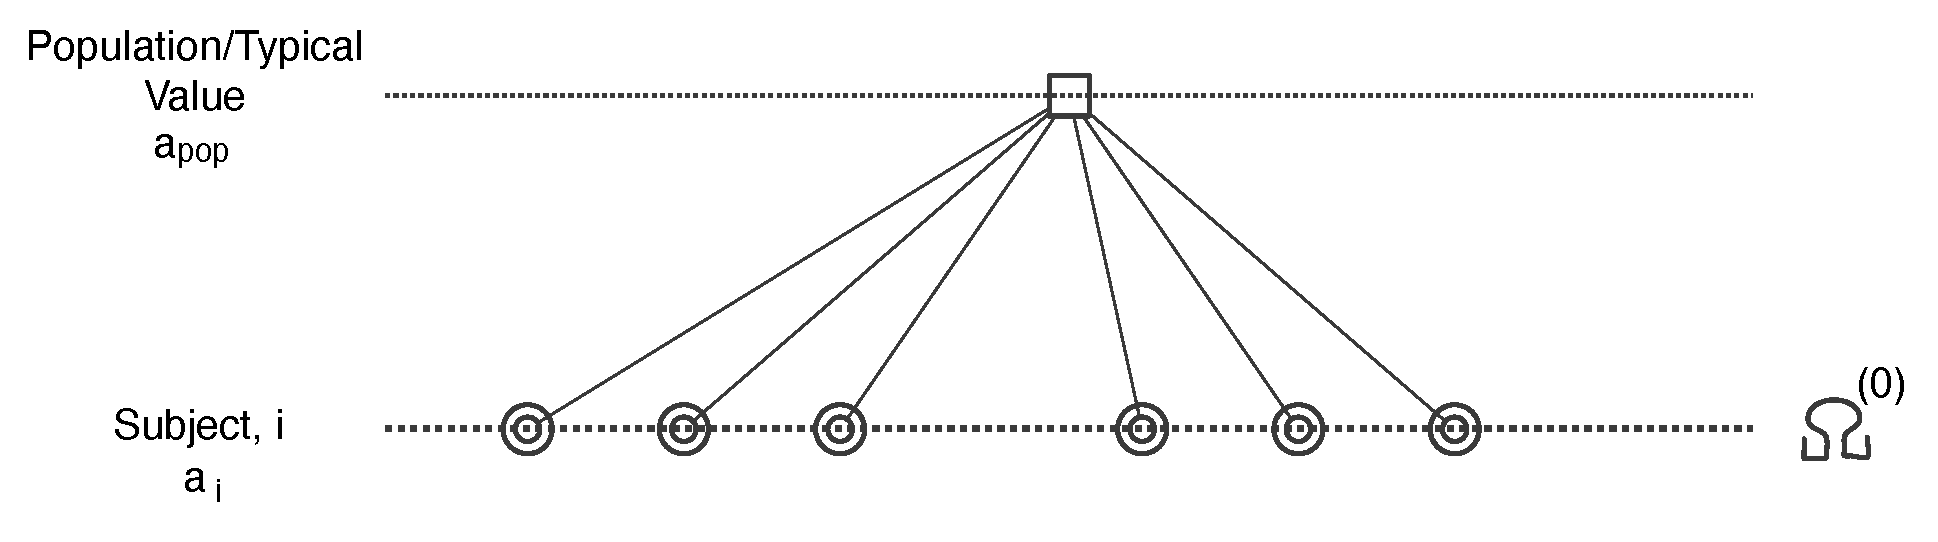
\includegraphics[width=130mm]{pics/IOV0}
 \caption{Inter-individual variability of the residual error parameter $a$. The nested hierarchical structure is identical to that of structural model parameters.}
 \label{fig:IOV0_residualError}
\end{figure}


%%%%%%%%%%%%%%%%%%%%%%%%%%%%%%%%%%%%%%%%%%%%%%%%%%%%%%%%%%%%%%%%%%
\subsubsection{Residual error model examples}
\label{subsec:modelExamples}
Currently, there is no library of residual error models but this might change in the future. All of the following residual error model examples and their different versions can be implemented in the present version of PharmML:
\begin{itemize}
\item
Constant/additive:
\begin{align*}
& y_{ij} = f_{ij} + a \; \epsilon_{ij}; \quad \epsilon_{ij} \sim N(0,1)  \\
\text{or} \quad & y_{ij} = f_{ij} + \epsilon_{ij}; \quad \epsilon_{ij} \sim N(0,\sigma^2)
\end{align*}
\item
Proportional or constant CV (CCV):
\begin{align*}
&y_{ij} =  f_{ij} + bf_{ij} \; \epsilon_{ij}; \quad \epsilon_{ij} \sim N(0,1)  \\
\text{or} \quad & y_{ij} =  f_{ij}(1+\epsilon_{ij}); \quad \epsilon_{ij} \sim N(0,\sigma^2)
\end{align*}
\item
Combined additive and proportional 1:
\begin{align*}
& y_{ij} =  f_{ij} + (a + bf_{ij}) \; \epsilon_{ij}; \quad \epsilon_{ij} \sim N(0,1)
\end{align*}
\item
Combined additive and proportional 2:
\begin{align*}
& y_{ij} =  f_{ij} + \sqrt{a^2 + b^2f_{ij}^2} \; \epsilon_{ij}; \quad \epsilon_{ij} \sim N(0,1)  \\
\text{or}  \quad & y_{ij} =  f_{ij} +  a\, \epsilon_{1,ij} + b f_{ij}\, \epsilon_{2,ij}; \quad \epsilon_{1,ij} \sim N(0,1); \quad \epsilon_{2,ij} \sim N(0,1);   \\
\text{or}  \quad & y_{ij} =  f_{ij} (1 + \epsilon_{1,ij}) + \epsilon_{2,ij}; \quad \epsilon_{1,ij} \sim N(0,\sigma_1^2); \quad \epsilon_{2,ij} \sim N(0,\sigma_2^2);
\end{align*}
\item
Power error model:
\begin{align*}
& y_{ij} = f_{ij} + b\,f_{ij}^c \; \epsilon_{ij}; \quad \epsilon_{ij} \sim N(0,1)
\end{align*}
\item
Combined additive and power error model 1:
\begin{align*}
& y_{ij} =  f_{ij} + (a + b f_{ij}^c) \; \epsilon_{ij}; \quad \epsilon_{ij} \sim N(0,1)
\end{align*}
\item
Combined additive and power error model 2:
\begin{align*}
& y_{ij} = f_{ij} + a\epsilon_{1,ij} + b f_{ij}^c \epsilon_{2,ij}; \quad \epsilon_{1,ij} \sim N(0,1); \quad \epsilon_{2,ij} \sim N(0,1)
\end{align*}
\item
Two (or more) types of measurements error model:
\begin{align*}
& y_{ij} = f_{ij} + \text{ASY}_j\epsilon_{1,ij} + (1-\text{ASY}_j) \epsilon_{2,ij}; \quad \epsilon_{1,ij} \sim N(0,\sigma_1^2); \quad \epsilon_{2,ij} \sim N(0,\sigma_2^2)
\end{align*}
\item
Two (or more) types of observations error model:
\begin{align*}
& y_{ij} = \text{TYP}_{ij} f_{1,ij} + (1-\text{TYP}_{ij}) f_{2,ij} + \text{TYP}_{ij}\epsilon_{1,ij} + (1-\text{TYP}_{ij}) \epsilon_{2,ij};  \\
&  \epsilon_{1,ij} \sim N(0,\sigma_1^2); \quad \epsilon_{2,ij} \sim N(0,\sigma_2^2)
\end{align*}
%\item
%Extended error model:
%
%y_{ij} = \left\{ \begin{array}{rcl}  f_{ij} + \epsilon_{1,ij}  & \mbox{for} & \text{TIME == 1 \&\& ID == 1} \\
%f_{ij} + \epsilon_{2,ij}  & \mbox{for} & \text{TIME == 2 \&\& ID == 1} \\
%\cdots \end{array}\right\} \quad \text{with} \quad
%\epsilon_{1,ij} \sim N(0,\sigma_1^2),\, \epsilon_{2,ij} \sim N(0,\sigma_2^2), \cdots
%
\end{itemize}
Main sources: \cite{NONMEM:2006aa} and \cite{POPIX:2013}.

\subparagraph{Note 1}
In the list above models are pulled together which have the same variance function.
\subparagraph{Note 2}
Models listed above are the most popular ones in use but the present PharmML 
structure allows for implementation of virtually any user-defined model. See 
section ref:XYZ for more examples and PharmML implementation.

%%%%%%%%%%%%%%%%%%%%%%%%%%%%%%%%%%%%%%%%%%%%%%%%%%%%%%%%%%%%%%%%%%
\subsection{Discrete data }
\label{subsec:DiscreteData}

The central piece of information to be provided when modeling discrete data is 
their distribution. While it is possible to encode in PharmML virtually any 
probability mass or density function explicitly, in few cases we can use the UncertML 
\cite{uncertml3:2014} and its extensive collection of distributions. 

The following sections are about the minimal information necessary to be 
implemented for most common types of discrete data models. It is important to note 
that we tried to stay generic rather then to provide the support for 
encoding of models in a particular tool. 

%%%%%%%%%%%%%%%%%%%%%%%%%%%%%%%%%%%%%%%%%%%%%%%%%%%%%%%%%%%%%%%%%%%%
\subsubsection{Count data}
\label{subsec:mmCountData}
An example for count data is the number of events of certain types, such as seizures, heart attacks and 
is typically modelled by the Poisson distribution. In the case of so called \textit{over-dispersed} 
data, i.e. when the variability is greater then what one would expect based on typical data sample, 
we have to resort to more complex models, such as negative binomial or zero-inflated Poisson model, 
see \ref{subsubsec:alternatives}.
Typically the minimal information to be provided consists of:
\begin{itemize}
\item
Type of observed variable -- discrete/count
\item
Count variable, e.g. $y$
\item
Parameters (see also Table \ref{tab:countDataModels})
\begin{itemize}
\item
Rate parameter $\lambda$, also called the Poisson 'intensity' $\lambda_{ij} = \lambda(t_{ij}, \psi_{ij})$, can be
\begin{itemize} %\addtolength{\itemsep}{-.95\baselineskip} 
\item
constant (\emph{homogenous Poisson process})
\begin{eqnarray}
\lambda(t_{ij}, \psi_{i}) = \lambda_{i} \nonumber
\end{eqnarray}
\item
a function of time (\emph{non-homogenous Poisson process})
\begin{eqnarray}
\lambda(t_{ij}, \psi_{i}) = \lambda_{0,i} + a_i t_{ij} \nonumber
\end{eqnarray}
\item
a function of additional regression variables, e.g. drug concentration linked to $\lambda$ via an Imax-model
\begin{eqnarray}
\lambda(t_{ij}, \psi_{i}) = \lambda_{0,i} \Big(1 - Imax_i \frac{C_i(t_{ij})}{IC_{50,i} + C_i(t_{ij})} \Big) \nonumber
\end{eqnarray}
\end{itemize}
\item
Overdispersion parameter, $\tau$ (NB model) %, section \ref{subsec:NBmodel})
\item
Dispersion parameter, $\delta$ (GP model) %, section \ref{subsec:GPmodel})
\item
Mixture probability, $\pi$ (PMIX$_2$ model) %, section \ref{subsec:PMIX2model})
\item
Zero probability, $p_0$ (ZIP model) %, section \ref{subsec:ZIPmodel})
\end{itemize}
\item
Probability mass function (PMF) with a link function. 
For example one can define 
\begin{itemize}
\item
the untransformed PMF, e.g.
\begin{eqnarray}
&& P(y_{ij}=k; \lambda) = \frac{\lambda^k \exp(-\lambda))}{k!} \nonumber
 \end{eqnarray}
\item
or log(Poisson-PMF) 
\begin{eqnarray}
&&	\log(P(y_{ij}=k;\lambda)) = -\lambda + k \log(\lambda) - \log(k!) \nonumber
\end{eqnarray}
%\item
%or explicit PMF definition
%\begin{itemize}
%\item
%PM -- Poisson -- parameter: $\lambda$
%\item
%ZIP -- Zero-inflated Poisson  -- parameters: $\lambda, p_0$
%\item
%GP -- Generalised Poisson -- parameters: $\lambda, \delta$
%\item
%PMIX -- Poisson with mixture distribution -- parameters: $\lambda_1,\lambda_2,\pi$
%\item
%NB -- Negative Binomial -- parameters: $\lambda, \tau$
%\end{itemize}
\end{itemize}
\item
Link function -- one from the list: $\{$\emph{identity}, \emph{log}, \emph{logit}, \emph{probit}$\}$. 
\item
Markovian dependence, see Sec.\ref{subsec:markovian}.
\end{itemize}


The following table gives an overview of common count data models encodable 
in \pharmml.

\begin{table}[htdp]
\centering  % centering table
\begin{tabular}{c c c c c}  
\hline\hline
Short  & Full Model 	& Distribution 	& Dependance 		& Markov \\ [-0.5ex]   
name  & 			& parameters 	& 			 	& order 	\\ [0.5ex]   
\hline
\multicolumn{5}{c}{equi-dispersed data}  \\[.1ex]
\hline
PS  		& Poisson 		& $\lambda$ 	& -- 		& -- 			 \\ [1ex] % & \textsection\ref{subsec:PMmodel} \\ [1ex]
PMAK 	& Poisson with 		& $\lambda_i$ 	& Markov 	& any order 	 \\ [-.5ex] % & \textsection\ref{subsec:PMAKmodel} \\[-.5ex]
		& Markov elements	&			&		& is supported \\[1ex]
\hline
\multicolumn{5}{c}{over-dispersed data}  \\[.1ex]
\hline
NB 		& Negative Binomial 	&  $\lambda, \tau$ 			& -- 	& -- \\ [1ex] % & \textsection\ref{subsec:NBmodel}
ZIP 		& Zero-Inflated Poisson 	& $\lambda, p_0$ 			& -- 	& -- \\ [1ex] % & \textsection\ref{subsec:ZIPmodel} \\ [1ex]
GP 		& Generalized Poisson 	& $\lambda, \delta$ 			& -- 	& -- \\ [1ex] % & \textsection\ref{subsec:GPmodel} \\ [1ex]
PMIX$_2$ & Poisson with 		& $\lambda_1, \lambda_2, \pi$ & -- 	& --  \\ [1ex] % & \textsection\ref{subsec:PMIX2model} \\[-.5ex]
  		& Mixture Distribution 	&  						&  	&  \\[1ex]
% [1ex] adds vertical space
\hline                          % inserts single-line
\end{tabular}
\caption{Overview of most popular count data models as used in pharmacometrics, based on \cite{Plan:2009fk}.
All of them are encodable in PharmML.}
\label{tab:countDataModels}
\end{table}%


\paragraph{Alternative models} 
\label{subsubsec:alternatives}
Poisson model listed above applies to equi-dispersed data only.
There is a number of alternative models which can handle over-dispersed data. 
Note, that the according PMF or log(PMF) has to be explicitly encoded in PharmML, see \cite{Plan:2009fk}:
\begin{itemize}%\addtolength{\itemsep}{-.95\baselineskip} 
\item
Zero-inflated Poisson model, ZIP
\begin{eqnarray}
P(y_{ij} = k; \lambda, p_0) =  \left\{ \begin{array}{rcl} p_0 + (1-p_0) e^{-\lambda} & \mbox{if} & k = 0 \\ 
(1-p_0)\frac{e^{-\lambda}\lambda^k}{k!} & \mbox{if} & k > 0 \end{array}\right. \nonumber
\end{eqnarray}
with $\lambda > 0$ and $p_0 \in [0,1]$
\item
Generalised Poisson model, GP
\begin{eqnarray}
P(y_{ij} = k; \lambda, \delta) &=& \frac{\lambda (\lambda + k \delta)^{k-1} e^{-\lambda - k\delta}}{k!} \nonumber
\end{eqnarray}
with $\lambda > 0$ and  $\delta \in [0,1]$
\item
Poisson model with mixture distribution, PMIX
\begin{eqnarray}
P(y_{ij} = k;\pi,\lambda_1,\lambda_2) &=& \pi \frac{e^{-\lambda_1} \lambda_1^k}{k!} + (1-\pi) \frac{e^{-\lambda_2} \lambda_2^k}{k!} \nonumber
\end{eqnarray}
with $\lambda_1, \lambda_2 > 0$ and $\pi \in [0,1]$
\item
Negative Binomial model, NB
\begin{eqnarray}
P(y_{ij} = k;\lambda,\tau) &=& \frac{\Gamma \big( k + \frac{1}{\tau} \big)}{k! \times \Gamma \big(\frac{1}{\tau} \big)} \times \Bigg( \frac{1}{1 + \tau \times \lambda} \Bigg)^{\frac{1}{\tau}} \times \Bigg(\frac{\lambda}{\frac{1}{\tau} + \lambda} \Bigg)^k \nonumber
\end{eqnarray}
with $\lambda, \tau > 0$.
%\item
%Poisson model with Markovian dependence, PMAK
%\begin{align}
% \lambda = \left\{ \begin{array}{rcl}
%			\lambda_1 & \mbox{for} & yp = 0 \\
%			\lambda_2 & \mbox{for} & yp \neq 0 \nonumber
%\end{array}\right. 
%\quad \text{and} \quad P(y=k; \lambda) = \frac{\lambda^k \exp(-\lambda)}{k!} \nonumber
%\end{align}
\end{itemize}

\subparagraph{Note 1} PharmML 0.4 supports the mathematical functions \textit{gammaln} 
-- logarithm of gamma function and \textit{factln} -- logarithm of the factorial.
\subparagraph{Note 2} Currently only the Poisson distribution is supported by UncertML, 
meaning that all other PMF's have to be implemented explicitly. The Negative Binomial distribution
is featured in UncertML as well but is using a different parametrisation and therefore cannot be used 
for our purposes.

%%%%%%%%%%%%%%%%%%%%%%%%%%%%%%%%%%%%%%%%%%%%%%%%%%%%%%%%%%%%%%%%%%%%
\subsubsection{Categorical data}
\label{subsec:mmCategoricalData}
The standard count data models, as presented in the previous section, are simpler to categorise 
and implement then the categorical ones. This is because for the former the definition of a probability 
mass function (PMF) and few parameters is sufficient. On the contrary the categorical models come 
with a vast variety of probability expressions, such as basic nominal and ordered models but also 
more complex once e.g. adjacent category models, continuation ratio 
models, latent continuous variable model and others. \cite{Paule:2012fk} provides an excellent 
overview of discrete models as used in pharmacodynamics.

Categorical model type deals with data organised in nominal (e.g. presence/absence of an event) 
or ordered (e.g. pain scale) categories. In the first case the probability for each category is defined. 
For the second case the cumulative or tail probabilities have to be defined. Furthermore, there are cases
when Markovian dependency and initial/conditional probabilities have to be considered.

Typically the minimal information to be provided consists of:
\begin{itemize}
\item
Nominal categorical data 
\begin{itemize}
\item
Set of categories, e.g. $\{0,1\}$ or $\{1,2,3\}$
\item
Category variable: e.g. $Y$
\item
Probability for each category
\begin{itemize}
\item
Binomial distribution, e.g. $P(Y=1) = p$ (for $Y \in \{0,1\}$) 
\item
Probabilities for the $k$ (or $k-1$) categories, here for $Y \in \{1,2,3\}$, 
\begin{eqnarray}
&&P(Y=1)=a1/(a1+a2+a3) \nonumber \\
&&P(Y=2)=a2/(a1+a2+a3)  \nonumber \\
&&P(Y=3)=1-P(Y=1)-P(Y=2) \nonumber
\end{eqnarray}
\end{itemize}
\item
or alternatively PMF using predefined distributions in UncertML -- available are following distributions: 
bernoulli, binomial, categorical.
\item
Markovian dependence, see Sec.\ref{subsec:markovian}
\item
Link function from the list $\{$\emph{identity}, \emph{log}, \emph{logit}, \emph{probit}$\}$
%\emph{loglog}, \emph{comloglog}--  {\color{red} \scshape{*}}last two link function have been introduced in the 0.4.1 version.\\
%-- ADD definition  {\color{red} \scshape{*}}\\
\end{itemize}
\item
Ordered categorical data
\begin{itemize}
\item
Set of categories, e.g. $\{0,1\}$ or $\{1,2,3\}$
\item
Category variable: e.g. $Y$
\item
Link function -- one from the list: $\{$\emph{identity}, \emph{log}, \emph{logit}, \emph{probit}, \emph{loglog}, \emph{comploglog}$\}$. 
\item
Probability for $k$ or $(k - 1)$ categories -- using one of the link functions. The possible options are 
\begin{itemize}
\item
Exact Cumulative  probability -- P(Y $\leq$ i), log(P(Y $\leq$ i)), logit(P(Y $\leq$ i)), probit(P(Y $\leq$ i)), loglog(P(Y $\leq$ i)), comploglog(P(Y $\leq$ i)) 
\item
Cumulative  probability -- P(Y$<$i), log(P(Y $<$ i)), logit(P(Y $<$ i)), probit(P(Y $<$ i)), loglog(P(Y $<$ i)), comploglog(P(Y $<$ i)), 
\item
Exact Tail probability  -- P(Y $\geq$ i), log(P(Y $\geq$ i)), logit(P(Y $\geq$ i)), probit(P(Y $\geq$ i)), loglog(P(Y $\geq$ i)), comploglog(P(Y $\geq$ i)) 
\item
Tail probability -- P(Y $>$ i), log(P(Y $>$ i)), logit(P(Y $>$ i)), probit(P(Y $>$ i)), loglog(P(Y $>$ i)), comploglog(P(Y $>$ i)) 
\end{itemize}

e.g. 
\begin{itemize}
\item
Cumulative probabilities, e.g. 
\begin{eqnarray}
&&P(Y\leq1)=a1/(a1+a2+a3) \nonumber \\
&&P(Y\leq2)=(a1+a2)/(a1+a2+a3) \nonumber \\
&&P(Y\leq3)=1-P(Y<=2) \nonumber
\end{eqnarray}
\item
Tail probabilities, e.g. 
\begin{eqnarray}
&& P(Y>1)=(a2+a3)/(a1+a2+a3) \nonumber \\
&& P(Y>2)=a3/(a1+a2+a3)  \nonumber \\ 
&& P(Y>3)=1-P(Y>2) \nonumber
\end{eqnarray}
\item
Cumulative logit probabilities, e.g. 
\begin{align}
& \text{logit}(P(Y\leq1))= \theta_1  \nonumber \\
& \text{logit}(P(Y\leq2))= \theta_1+\theta_2  \nonumber \\
& \text{logit}(P(Y\leq3))=1  \nonumber
\end{align}
\end{itemize}
\item
Markovian dependence, see Sec.\ref{subsec:markovian} for definition and examples.
\end{itemize}
\end{itemize}

\paragraph{Complex categorical data} The proposed PharmML structure allows to encode 
other popular models useful in pharmacometrics \cite{Dobson:2002uq}, for example
\begin{itemize}
\item
Complementary log-log models
\begin{align}
& \log\{-\log[P(y=j)]\} = \beta_0 + \beta_1 x \nonumber
\end{align}
\item
Continuation ratio model
\begin{align}
& \text{logit}\Big[\frac{P(y=j) }{ \sum_{i =j+1}^{J} P(y=i) } \Big] = b + \sum_{j = 1}^{N} \beta_j x_j \nonumber
\end{align}
\item
Adjacent category logit model
\begin{align}
& \log\Big[\frac{P(y=j) }{ P(y=j+1) } \Big] = \sum_{j = 1}^{N} \beta_j x_j \nonumber
\end{align}
\item
Complex logit functions (based on \cite{Girard:1998fk})
\begin{align}
& \log \Big[\frac{P(n_j=r | n_{j-1}=q) }{ 1 - \sum_{j\in \{0,2\}} P(n_j=k | n_{j-1} = q)} \Big] = p_{rqkq} \nonumber
\end{align}
\end{itemize}


%\paragraph{Build-in categorical models} Even though such complex models as shown above are implementable
%explicitly in \pml 
%\cite{Dobson:2002uq}, for example
%\begin{itemize}
%\item
%
%\item
%
%\end{itemize}


%%%%%%%%%%%%%%%%%%%%%%%%%%%%%%%%%%%%%%%%%%%%%%%%%%%%%%%%%%%%%%%%%%%%
\subsubsection{Time-to-event data}
In this case the observation is time until an event occurs, which can be unique or repeated.
The model is fully described by defining the the survival or hazard function. Following minimal information 
needs to provided to ensure lossless encoding of this model type.
\begin{itemize}
\item
Type of observed variable -- discrete/time-to-event
\item
One of the probability distribution defining functions
\begin{itemize}
\item
Hazard function, $h(t; \psi_i)$ or
\item
Survival function $S(t;\psi_i)$
\end{itemize}
\item
Type of censoring
\begin{itemize}
\item
Right censoring -- right censoring time 
\item
Interval censoring -- interval length
\end{itemize}
\item
Maximum number of possible events.
\end{itemize}


%%%%%%%%%%%%%%%%%%%%%%%%%%%%%%%%%%%%%%%%%%%%%%%%%%%%%%%%%%%%%%%%%%%%
\subsubsection{Markovian dependence}
\label{subsec:markovian}

%\begin{figure}[htb!]
%\centering
%  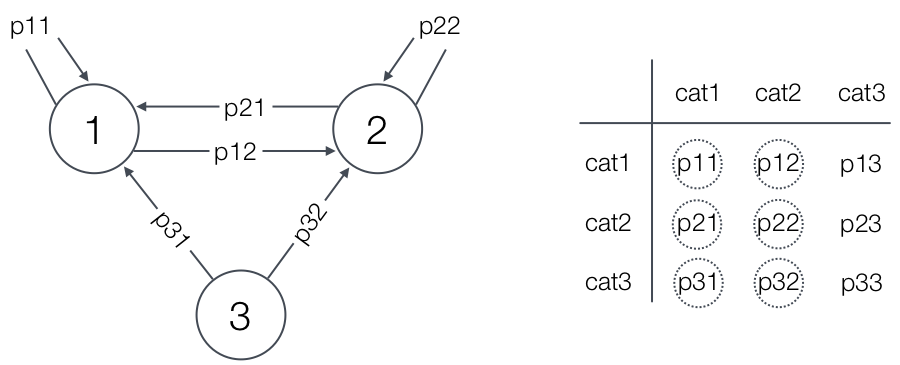
\includegraphics[width=105mm]{pics/markovDependency}
% \caption{An example for Markovian dependence state network.}
% \label{fig:markovDependency}
%\end{figure}
%

To define Markovian dependence in any of those models above, one needs to specify:
\begin{itemize}
\item
State variables as one of the following
\begin{itemize}
\item
Initial state variable, $yinit$
\item
Current state variable, $y$
\item
Previous state variable, $yp$
\end{itemize}
\item
Probability transitions or their alternative transformed forms for a discrete-time models Markov process, e.g.
\begin{align}
& \text{logit}(P(y<=1 | yp=1)) = a11 \nonumber \\
& \text{logit}(P(y<=2 | yp=1)) = a11 + a12\nonumber
\end{align}
with $y$ -- current state, $yp$ -- previous state.
\item
Transition rates for a continuous-time Markov process, \cite{LavielleBook:2014}, e.g.
\begin{align}
& \rho_{1,2}(t) = \exp(a_i+b_i t)  \nonumber \\
& \rho_{2,1}(t) = \exp(c_i+d_i t) \nonumber 
\end{align}
\item
Probability distribution of the initial states, $yinit1, yinit2, ...$ -- 'distribution of first observations'
% -- is equal to the row vector of the stochastic matrix.
\item
Markov order.
\end{itemize}








%\paragraph{Covariate model}
%Covariate model is barely covered so far. See also \cite{Keizer:2011aa}. Missing are following features:\\
%For categorical covariates:\\
%-- categorical distribution of categorical covariates \\
%---- estimating categorical distribution from external data file \\
%---- sampling from known categorical distribution \\
%---- clusters of categorical covariates \\
%For continuous covariates:\\
%-- power-normal distribution for continuous covariates \\
%---- estimating parameters $\lambda$,$\mu$,$\sigma$ from external data file \\
%---- sampling from known power-normal distribution \\
%---- conditional distribution of continuous covariates \\
%------ none \\
%------ defined \\
%------ to be estimated \\
%---- selecting criteria for continuous covariates \\
%---- dependent distribution of continuous covariates \\
%---- correlated continuous covariates \\
%For both types: \\
%-- selection/exclusion criteria missing \\
%
%\subsection{Observation model}
%- Name\\
%- Units\\
%- Observation types - continuous/discrete\\
%- Symbol of predicted output\\
%
%\subsection{Task model}
%-- Combination of tasks, e.g.\\
%1. estimate distribution of covariate from experimental data\\
%2. Simulation task using the estimated PDF
%
%
%\subsection{Not covered so far}
%- correlation of residual errors \\
%---- number models of relevant models identified and described in Use Case document\\
%


%%%%%%%%%%%%%%%%%%%%%%%%%%%%%%%%%%%%%%%%%%%%%%%%%%%%%%%%%%%%%%%%%
%%%%%%%%%%%%%%%%%%%%%%%%%%%%%%%%%%%%%%%%%%%%%%%%%%%%%%%%%%%%%%%%%
\chapter{Trial design model}
\label{sec:CTS}
\label{maths:epoch-defn}

%%%%%%%%%%%%%%%%%%%%%%%%%%%%%%%%%%%%%%%%%%%%%%%%%%%%%%%%%%%%%%%%%
\section{Introduction}

In tools such as NONMEM and MONOLIX it has been common practice to encode the trial design in a data file.
More specifically parts of the overall problem, e.g. the structural model and the parameters are explicitly
encoded in the model file, while other, design related, parts are encoded in the data file. This implies
that the software tool, when processing the data file, must associate the data items with model variables
in order to recognise all characteristics of a study, such as subject-specific measurement time points
and values, covariates, variability levels, etc. This has clear disadvantages for simulation purposes,
because it means that when wanting to change only the design, the data file has to be changed, an error
prone and time consuming work. This is clearly not an ideal situation and PharmML addresses this issue.

It is important to stress that we have based a major part of the trial design on one of the standards 
developed by CDISC "a global, open, multidisciplinary, non-profit organisation that has established 
standards to support the acquisition, exchange, submission and archive of clinical research data 
and metadata" \cite{CDICS:2013}. Over the recent years, this organisation has worked out a set of 
standards widely used in the medical and pharmaceutical research, both in academic and commercial centres. 
Using this standard gives us the reassurance that \pharmml will be able
to represent all trial structures that we are likely to encounter. 


\subsection{Sources of clinical data}

Clinical trials are carefully structured and can vary considerably in
their complexity. Typically, a trial will have one or more arms with
each arm containing one or more treatment regimens and observation
protocols. Individuals are then allocated to each arm from a population
of subjects who have been screened for their suitability to participate
in the trial. In \pharmml we describe the structure and population of a
trial explicitly in a dedicated section. This differs from some other
approaches, but we feel it makes the clinical trial much clearer to
document and easier to encode computationally.


%Typically, in tools such as NONMEM and MONOLIX, the trial design is
%encoded within a tabular data-file. This file contains dosing
%information, covariates and experimental observations for each
%individual in the trial. In addition the definition of the structure
%of the clinical trial is also embedded into this table, meaning that
%the data-file contains a lot of redundant information.

The clinical data comes usually from different sources (and formats) and 
in \pharmml we distinguish this information by separating it into the following three
classes of data dependent on their origin\footnote{It is interesting to note that the developers of
PharML had a similar insight and organised data in a similar
way \cite{NLMEcons:2008}.}:
%
\begin{description}
\item[Population] The attributes of the individuals in the study: the
  population in the population model. Each individual has a weight,
  an age, a gender and numerous other properties that may or may not
  be modelled as covariates in a given model. Importantly, the 'arm' 
  membership of every subject/patient is part of this information.
  In addition, these properties may change over time. 
\item[Dosing] When and how a drug or drugs are administered to the
  individuals in the trial.
\item[Measurements] These are the observations taken from each
  individual at specific times during the study. Such measurements
  provide the objective data used during parameter estimation and are
  typically the outputs calculated during a simulation.
\end{description}

%%%%%%%%%%%%%%%%%%%%%%%%%%%%%%%%%%%%%%%%%%%%%%%%%%%%%%%%%%%%%%%%%
\section{Trial Design}

By separating out these classes of information you can see that the
information we need to define for a clinical trial is as follows:
%
\begin{description}
\item[Structure] The organisation of the trial, how the subjects
  are grouped into different treatment groups and what the dosing
  regimen is within these treatment groups.
\item[Population] As above, the properties specific to the individuals,
  including those that vary over time.
\item[Individual Dosing] This is related to the treatment regimens
  described in the trial structure, but describes the dosing history
  for each individual in the study.
\end{description}
%
The measurement data is then used exclusively for estimation and
is encoded in the third major building block of \pharmml, in the 'Modelling 
Steps'.

%%%%%%%%%%%%%%%%%%%%%%%%%%%%%%%%%%%%%%%%%%%%%%%%%%%%%%%%%%%%%%%%%
\subsection{Structure}
\label{subsec:TrialStructure}

To define the Trial Structure we have reused, almost verbatim, the
CDISC Study Design Model \cite{CDISC:2011a}, which is an
XML representation of a clinical trial. Figure \ref{fig:CellSegmentEpochArmEvent_concept}
below shows how the CDISC trial structure is organised. It has six main components:
\begin{description}
\item[Epoch] The epoch defines a period of time during the study which
  has a purpose within the study. For example a washout or a treatment
  window. In CDISC Epochs can describe screening or follow-up periods,
  which are out of the scope of \pharmml. An epoch is usually defined
  by a time period.
\item[Arm] The arm represents a path through the study taken by a
  subject. An arm is composed of a study cell for each epoch in the study.
\item[Cell] The study cell describes what is carried out during an
  epoch in a particular arm. There is only one cell per epoch.
\item[Segment] The segment describes a set of planned observations and
  interventions, which may or may not involve treatment. Note that in
  \pharmml our definition is more limited and we only describe
  treatments. A segment can contain one or more activities.
\item[Activity] The activity is an action that is taken in the
  study. Here it is typically a treatment regimen or a washout.
\item[StudyEvent] A study event describes the collection of
  information about a particular individual. In CDISC this can be
  information captured during screening or other non-treatment phases
  of the clinical trial. But here we restrict it to capturing
  observations during the treatment. In \pharmml this is how we
  capture occasions.
\end{description}
\begin{figure}[htb]
\centering
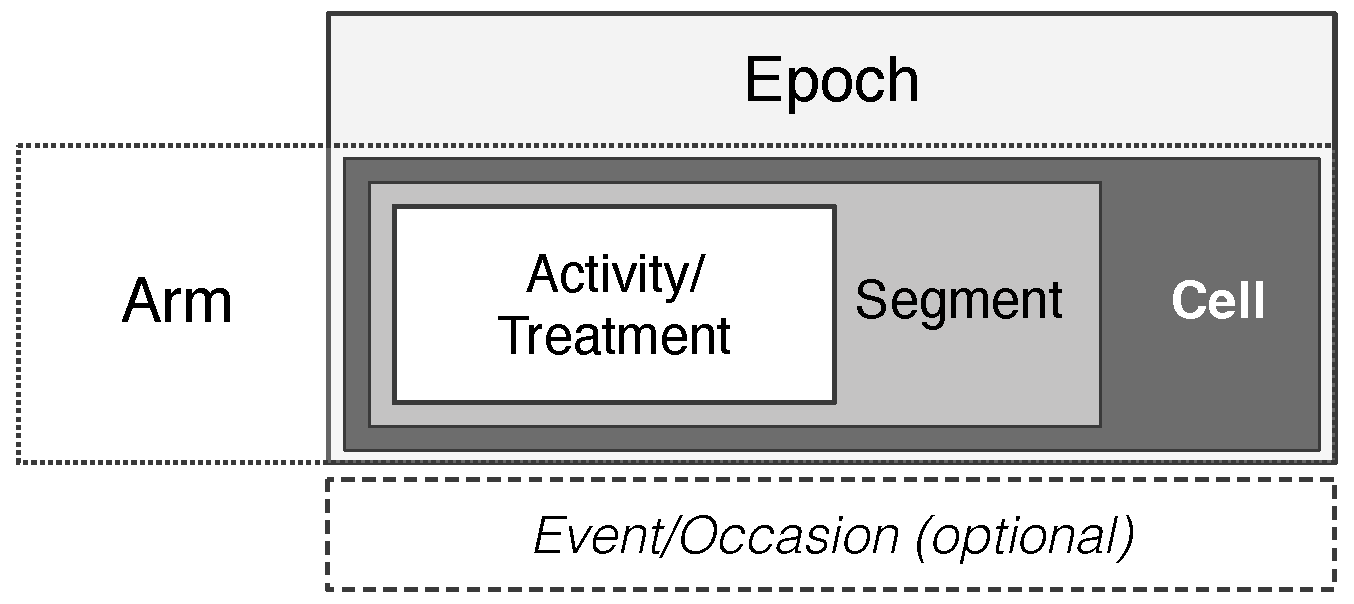
\includegraphics[height=0.2\textheight]{pics/CellSegmentEpochArmEvent_concept}%
\caption{Overview of the basic concept of the Trial Structure: arm,
epoch, event and a cell with segment and activity/treatment as used in the CDISC Study
  Design Model. See the next figure for an example.}
\label{fig:CellSegmentEpochArmEvent_concept}
\end{figure}
\begin{figure}[htb]
\centering
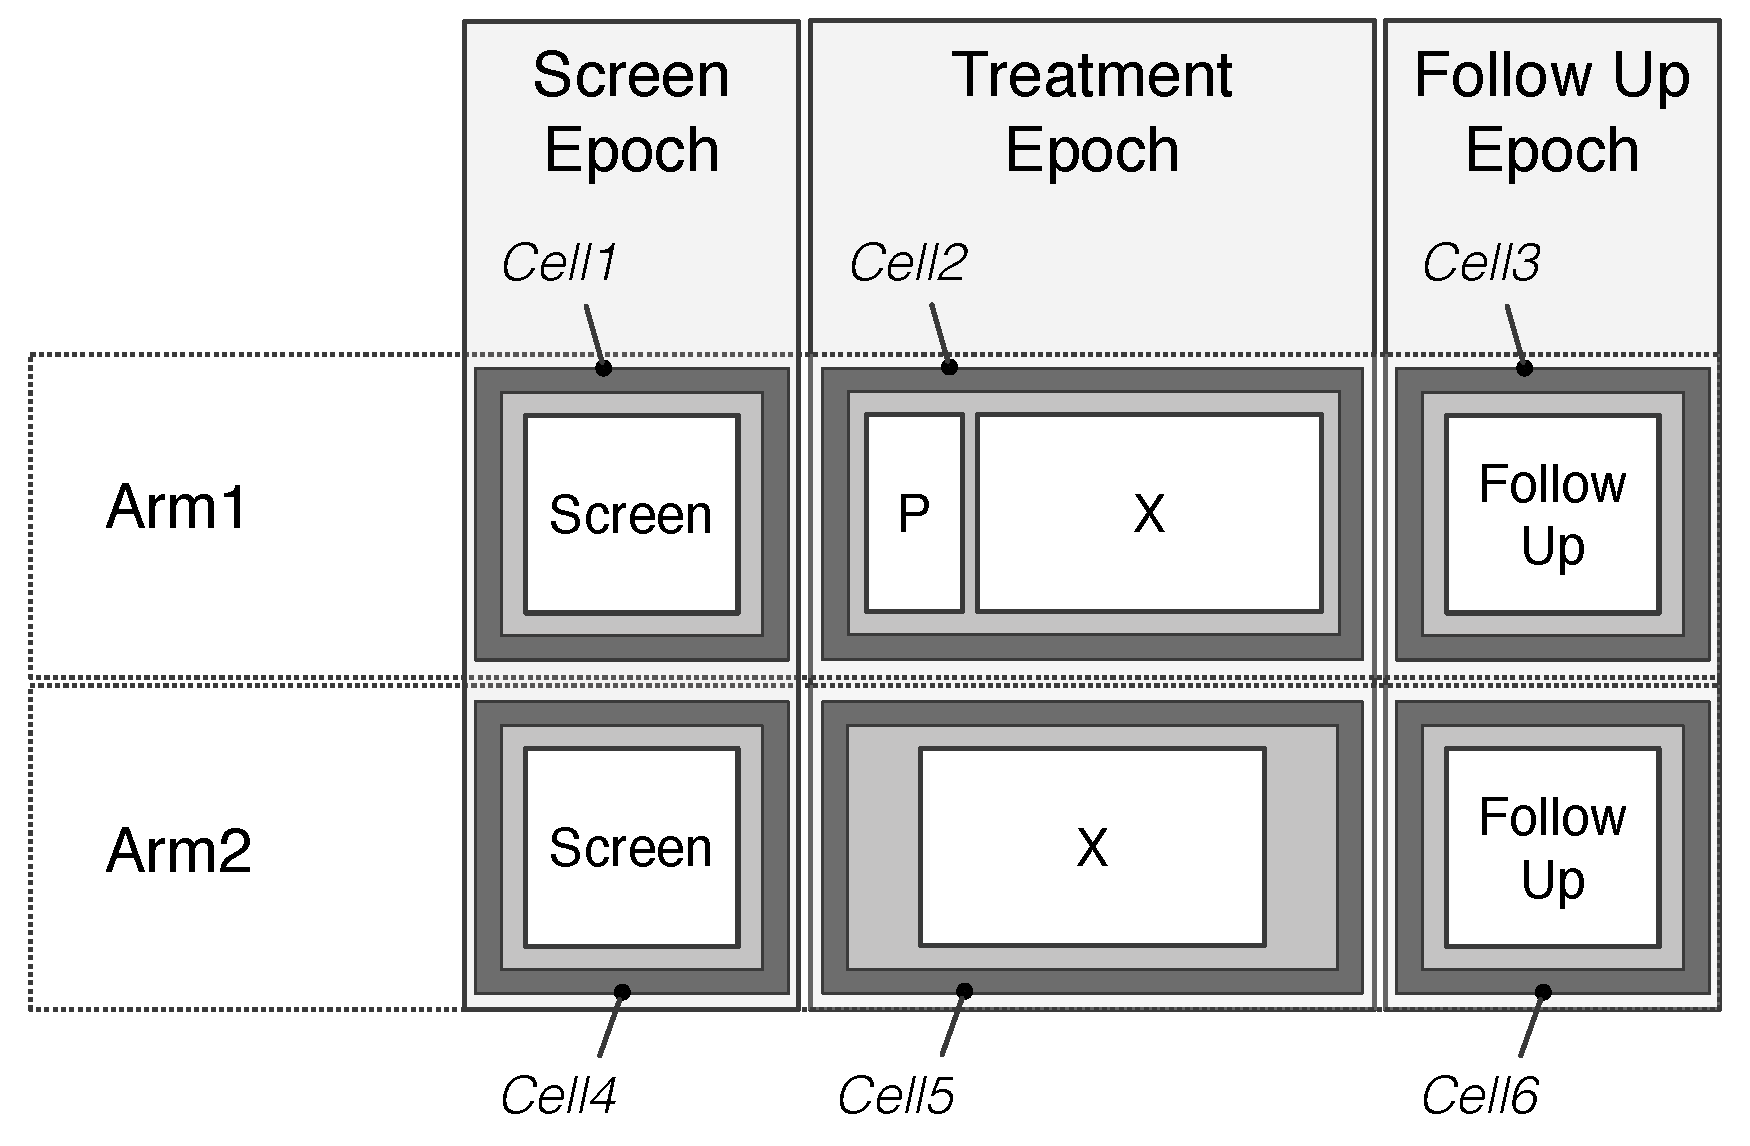
\includegraphics[height=0.375\textheight]{pics/templateTrialDesign.pdf}%
\caption{An example of a study with two arms and three epochs: Screen,
Treatment and Follow Up. A segment can contain more then one Activity/Treatment
as can be seen in \emph{Cell2} with one Pre-Treatment \emph{P} and one Treatment \emph{X}.
In this particular example no Event/Occasion is specified.}
\label{fig:templateTrialDesign}
\end{figure}
Figure \ref{fig:templateTrialDesign} shows one such example of a hypothetical trial
consisting of two arms and three epochs: \emph{Screen}, \emph{Treatment} and
\emph{Follow Up}. There are accordingly six cells and segments, each consisting of one
or two activities. \emph{Cell2} has the most complex structure carrying two
subsequent treatments, Pre-Treatment \emph{P} and Treatment \emph{X}. In this case
no Events/Occasions are specified which is an optional element in the design.

Examples of how a trial design is encoded in \pharmml can be found in
the examples (see chapter \ref{chap:worked-egs}).

\paragraph{Variability}
There is one aspect regarding the random variability worth mentioning
here. The \xelem{Population} block carries the information about subject 
level variability and those variability levels above the subject, see next section for more details.  
In the \xelem{Structure} element we encode the variability which is located below the
subject. This is typically known as \textit{inter-occasion variability} but deeper levels
are allowed in theory. The reader is referred to the section \ref{sec:variabilityModel} where the 
full nested hierarchy of the random variability discussed in detail.


%%%%%%%%%%%%%%%%%%%%%%%%%%%%%%%%%%%%%%%%%%%%%%%%%%%%%%%%%%%%%%%%%
\subsection{Population}
\label{subsec:TrialPopulation}

This is the second major element of the trial design description where we:
\begin{itemize}
\item
describe the individuals in the study
\item
describe their attributes (such as weight, gender, etc.)
\item
assign them to an arm of the study, but also
\item
indicate if variability at and/or below the subject level is to be defined, which is the case in the majority of models (if omitted
then this means that we explicitly consider a setup without any random variability,
which is the case for the na\"{\i}ve pooled data method), and
\item
indicate their country or centre membership to define higher levels of variability above the subject level.
\end{itemize}
We define the possible attributes of all individuals using the \emph{IndividualTemplate} block and then map
each individual to this template using a \emph{Dataset} block.

%\begin{description}
% \item[]
%
% \item[Epoch]
%
% \item[Epoch]
%
%\end{description}

%%%%%%%%%%%%%%%%%%%%%%%%%%%%%%%%%%%%%%%%%%%%%%%%%%%%%%%%%%%%%%%%%
\subsection{Individual dosing}
\label{subsec:TrialSIndivDosing}

The two previous sections on \emph{Structure} and \emph{Population} described information,
which is sufficient to encode e.g. a simple simulation task. Specifically, when the dosing is 
equal among the patients then this can be encoded in the \emph{Structure} part of the schema with
one or more dose amounts and one or more dosing times for all. However, in most cases, especially
when we deal with real clinical data this is not so straighforward. Every patient will have its own specific 
amounts and dosing times.

For an estimation task we always need to provide experimental data for each dosing activity 
relevant to the particular case. With the current structure we can provide individual dosing 
information for every dosing activity defined in the \emph{Structure} part (see \ref{subsec:TrialStructure}).

The structure of this part is similar to that used for \emph{Population} in that first
a table template is defined with all relevant columns, i.e. \emph{ID}, \emph{TIME}, and \emph{DOSE},
which is then populated with individual dosing data. 


%%%%%%%%%%%%%%%%%%%%%%%%%%%%%%%%%%%%%%%%%%%%%%%%%%%%%%%%%%%%%%%%%%
%\subsection{PharmML implementation}
%\label{subsec:TrialSIndivDosingPharmML}
%
%Dependent on the task to be implemented, the information to be stored
%in the Trial Design block will differ. For example an estimation task requires all three
%elements discussed above, which in \pharmml have the intuitive names
%\xelem{Structure}, \xelem{Population} and \xelem{IndividualDosing}
%(see figure \ref{fig:simEstTasks_trialList}). For a simulation task only the first two are
%necessary.
%
%
%\begin{figure}[htb]
%\centering
%\includegraphics[width=0.7\linewidth]{pics/simEstTasks_trialList}%
%\caption{PharmML building blocks used in the definition of a trial design.}
%\label{fig:simEstTasks_trialList}
%\end{figure}


%%%%%%%%%%%%%%%%%%%%%%%%%%%%%%%%%%%%%%%%%%%%%%%%%%%%%%%%%%%%%
%\begin{figure}[htbp!]
%\centering
%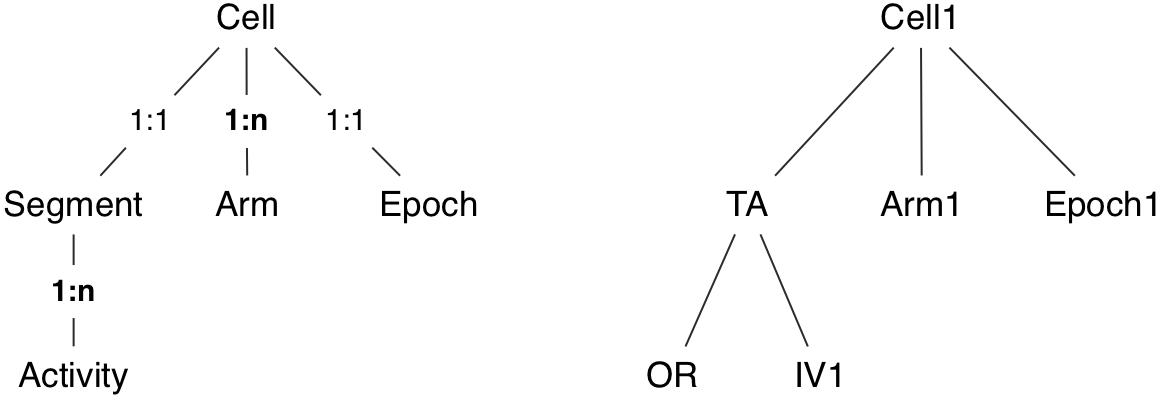
\includegraphics[width=0.8\linewidth]{../pics/cellHierarchy2}
%\caption{General cell hierarchy (left); The root of the hierarchy is the cell which can contain one segment, one epoch and multiple arms. The segment element can have multiple child elements, the activities e.g. treatments or a washout. (right) An example of how it is applied in this example.}
%\label{fig:cellHierarchy}
%\end{figure}

%\section{Design elements and examples}
%\label{sec:CTS_exampleSection} % KEEP THIS LABEL!!!!!!
%The default working mode, as mentioned above, is when all the study characteristics are encoded in the data file. Alternatively, PharmML offers a very flexible structure for the setup of clinical trials. Using only a few basic elements the modeller can compose several types of designs, including parallel design and crossover designs with or without washout or run-in period\footnote{\textit{Run-in} -- do be continued. Definition after \cite{Iverson:2007fk}}, see Figure \ref{fig:CTSfigure1} for examples. The basic elements are:
%
%\begin{itemize}
%\item
%%\textit{Dosing}
%%\begin{itemize}
%%\item
%%one or multiple dosing events can be defined
%%\item
%%dosing type: single dose, sequence/repeated or steady-state dosing
%%\item
%%type of administration: bolus or infusion
%%\item
%%target compartment/variable
%%\item
%%amount and/or infusion rate
%%\item
%%dosing times
%%\end{itemize}
%%\item
%\textit{Treatment} -- describes dosing related data
%\begin{itemize}
%\item
%Administration/dosing type, \textit{Bolus} or \textit{Infusion}, as single value or a sequence
%\item
%Dosing Times -- as single value or a sequence
%\item
%Dose Amount -- as single value or a sequence
%\item
%Dosing target
%\begin{itemize}
%\item
%Target variable (indicates the target compartment) -- for ODE coded structural models, e.g. $Ad$ the drug amount in the depot compartment (see section \ref{sec:structuralModel})
%\item
%Dose variable -- for explicit algebraic equations with a dose amount variable, e.g. $D$ as in $C(t)= \frac{D}{V}e^{-k(t-t_D)}$
%\end{itemize}
%\end{itemize}
%\item
%\textit{Treatment Epoch\footnote{\textit{Epoch} -- Interval of time in the planned conduct of a study. An epoch is associated with a purpose (e.g., screening, randomization, treatment, follow-up), which applies across all arms of a study. NOTE: Epoch is intended as a standardised term to replace: period, cycle, phase, stage. Definition after \cite{CDICS:2011}}} -- basic time interval within a study
%\begin{itemize}
%\item
%Epoch name, e.g. \textit{Treatment\_A} or \textit{Washout}\footnote{\textit{Washout} -- A period in a clinical study during which subjects receive no treatment for the indication under study and the effects of a previous treatment are eliminated (or assumed to be eliminated).} or \textit{Run-in}
%\item
%\textit{Start time} and \textit{end time} of an epoch -- this sets reference time frame for any possible occasion within an epoch
%\item
%Occasion(s) -- defined by
%\begin{itemize}
%\item
%\textit{start time} and \textit{end time} of each occasion relative to epoch time frame
%\item
%level identifier
%\end{itemize}
%\end{itemize}
%\item
%\textit{Group} -- basic grouping structure for subjects usually containing one or more treatment epochs
%\begin{itemize}
%\item
%a sequence of epochs for a number of subjects, e.g. [\textit{Epoch\_A}, \textit{Washout}, \textit{Epoch\_B}]
%\item
%number of subjects
%\end{itemize}
%\end{itemize}
%
%\paragraph{Note 1} The name of a particular trial design, e.g. \textit{parallel} or \textit{crossover with washout} is not part of the language. It can be provided as annotation of the trial design model using an appropriate ontology.
%\paragraph{Note 2} The 'Washout' epoch means complete reset of all variables and is defined without start and end times, but this restrictions will be released in an upcoming specification.
%\paragraph{Note 3} The support for variability levels is limited in this specification of PharmML. More specifically, it can only encode occasions definable using start and end times for each occasion. Levels above the subject reference level, such as 'country' or 'centre' cannot be encoded.
%


%\begin{figure} % [htb!]
%\centering
%\begin{tabular}{c}
% \includegraphics[width=140mm]{ClinicalDesignPatterns_version3}
% \end{tabular}
%\caption{Examples for basic clinical trial design types and configurations. In general any combination of the basic structural elements, i.e. \textit{Dosing}, \textit{Treatment}, \textit{Treatment Epoch} and \textit{Group}, can be created. Based on \cite{Lavielle:2012} and \cite{Wang:2006}.}
%\label{fig:CTSfigure1}
%\end{figure}


%%%%%%%%%%%%%%%%%%%%%%%%%%%%%%%%%%%%%%%%%%%%%%%%%%%%%%%%%%%%%%%%%
%\subsection{Example 1 -- Basic crossover with washout}
%This example describes a crossover design\footnote{\textit{Crossover design} -- Each subject is allocated to a sequence of treatments across a number of treatment periods. Within crossover trials, sequences can include all possible treatments or a subset of these (incomplete block). Definition after \cite{CDICS:2011}} with washout, see example F in Figure \ref{fig:CTSfigure1}.
%
%\subsubsection{Trial design model}
%
%-- Treatment definition
%\begin{align*}
%Treatment\_A: & AdministrationType = \text{[OR bolus, IV bolus]}  \\
%& DoseTime = [6:24:72, 0:24:72]   \\
%& DoseSize = [50, \;\;100]   \\
%& DoseVariable = \text{[D, \;\;D]}  \\
%Treatment\_B: & AdministrationType = \text{OR bolus}  \\
%& DoseTime = 0:24:72   \\
%& DoseSize = 150   \\
%& DoseVariable = \text{D}
%\end{align*}
%
%-- Treatment Epoch definition
%\begin{align*}
%Epoch\_1: & Treatment\_A  \\
%& TreatmentStart = 0  \\
%& TreatmentEnd = 100  \\
%Epoch\_2: & Treatment\_B  \\
%& TreatmentStart = 0  \\
%& TreatmentEnd = 100  \\
%Epoch\_3: & Washout
%\end{align*}
%
%-- Group definition
%\begin{align*}
%Group 1: 	& TreatmentSeq = \text{[Epoch\_1, Epoch\_3, Epoch\_2]}	 \\
%			& GroupSize = 40		 \\
%Group 2: 	& TreatmentSeq = \text{[Epoch\_2, Epoch\_3, Epoch\_1]}  \\
%			& GroupSize = 60
%\end{align*}
%
%
%%%%%%%%%%%%%%%%%%%%%%%%%%%%%%%%%%%%%%%%%%%%%%%%%%%%%%%%%%%%%%%%%
%\subsection{Example 2 -- Complex crossover trial with washout, 4 groups}
%See example H in Figure \ref{fig:CTSfigure1}.
%
%\subsubsection{Trial design model}
%
%-- Treatment definition
%\begin{align*}
%T1: & AdministrationType = \text{[OR1, OR2, IV]}  \\
%& DoseSize = [50 \;\;\;100 \;\;\;100];   \\
%& DoseTime = [6:24:72, 0:24:72, 12:24:72];   \\
%& DoseVariable = \text{[D, \;\;D, \;\;D]}  \\
%T2: & AdministrationType = \text{OR1}  \\
%& DoseSize = 150;   \\
%& DoseTime = [0:24:72];    \\
%& DoseVariable = \text{D}  \\
%T3: & AdministrationType = \text{OR2}  \\
%& DoseSize = 150;   \\
%& DoseTime = [0:24:72];   \\
%& DoseVariable = \text{D}  \\
%T4: & AdministrationType = \text{IV}  \\
%& DoseSize = 150;   \\
%& DoseTime = [0:24:72];   \\
%& DoseVariable = \text{D}
%\end{align*}
%
%
%-- Treatment Epoch definition
%\begin{align*}
%Epoch\_1: & T1  \\
%& TreatmentStart = 0  \\
%& TreatmentEnd = 100  \\
%Epoch\_2: & T2  \\
%& TreatmentStart = 0  \\
%& TreatmentEnd = 100  \\
%Epoch\_3: & T3  \\
%& TreatmentStart = 0  \\
%& TreatmentEnd = 100  \\
%Epoch\_4: & T4  \\
%& TreatmentStart = 0  \\
%& TreatmentEnd = 100  \\
%Epoch\_5: & Washout
%\end{align*}
%
%
%-- Group definition
%\begin{align*}
%Group 1: 	& TreatmentSeq = \text{[Epoch\_1, Epoch\_5, Epoch\_2, Epoch\_5, Epoch\_3]}	 \\
%			& GroupSize = 40		 \\
%Group 2: 	& TreatmentSeq = \text{[Epoch\_2, Epoch\_5, Epoch\_3, Epoch\_5, Epoch\_4]}  \\
%			& GroupSize = 40		 \\
%Group 3: 	& TreatmentSeq = \text{[Epoch\_4, Epoch\_5, Epoch\_1, Epoch\_5, Epoch\_2]}	 \\
%			& GroupSize = 60		 \\
%Group 4: 	& TreatmentSeq = \text{[Epoch\_4, Epoch\_5, Epoch\_3, Epoch\_5, Epoch\_2]}  \\
%			& GroupSize = 60
%\end{align*}





%%%%%%%%%%%%%%%%%%%%%%%%%%%%%%%%%%%%%%%%%%%%%%%%%%%%%%%%%%%%%%%%%
%\subsubsection{To-Do list}
%
%\paragraph{Crossover - other aspects not covered yet}
%- 2x2 -- covered already \\
%- p x q -- see Table 2 in \cite{Wang:2006} \\
%- Latin square 3x3 \& 4x4
%
%
%%%%%%%%%%%%%%%%%%%%%%%%%%%%%%%%%%%%%%%%%%%%%%%%%%%%%%%%%%%%%%%%%
%\paragraph{Factorial design}
%In a factorial design two or more treatments are evaluated simultaneously through the use of varying combinations of the treatments. The simplest example is the 2x2 factorial design in which subjects are randomly allocated to one of the four possible combinations of two treatments, A and B say. These are: A alone; B alone; both A and B; neither A nor B. Source: \cite{EMA:1998}\\
%- no example available
%
%\paragraph{Other aspects of factorial design to be considered}
%- 2x2, Ix J x K, unbalanced, 'complicated'
%
%
%%%%%%%%%%%%%%%%%%%%%%%%%%%%%%%%%%%%%%%%%%%%%%%%%%%%%%%%%%%%%%%%%
%\paragraph{Cohort study}
%Study of a group of individuals, some of whom are exposed to a variable of interest, in which subjects are followed over time. Cohort studies can be prospective or retrospective. [AMA Manual of Style] See also prospective study.
%
%%%%%%%%%%%%%%%%%%%%%%%%%%%%%%%%%%%%%%%%%%%%%%%%%%%%%%%%%%%%%%%%%
%\paragraph{Prospective study}
%Investigation in which a group of subjects is recruited and monitored in accordance with criteria described in a protocol.
%
%
%%%%%%%%%%%%%%%%%%%%%%%%%%%%%%%%%%%%%%%%%%%%%%%%%%%%%%%%%%%%%%%%%
%\paragraph{Survival}
%Observe N subjects until at most time T (censored observations). Alternatively observe N subjects until at least R events occur.\\
%- no example available
%
%
%%%%%%%%%%%%%%%%%%%%%%%%%%%%%%%%%%%%%%%%%%%%%%%%%%%%%%%%%%%%%%%%%
%\paragraph{Observational}
%Subjects are not randomly allocated to treatment.\\
%- no examples available
%
%
%%%%%%%%%%%%%%%%%%%%%%%%%%%%%%%%%%%%%%%%%%%%%%%%%%%%%%%%%%%%%%%%%
%\paragraph{Dose escalation Methods in Phase I, \cite{Le-Tourneau:2009fk}}
%-- Rule-based designs: \\
%Traditional 3+3 design, Accelerated titration designs, Pharmacologically guided dose escalation\\
%Model-based designs: \\
%-- Modified continual reassessment method, Escalation with overdose control, Time-to-event continual reassessment method, EffTox -- efficacy and toxicity method, TriCRM -- an adaptive continual reassessment method that considers three potential trial outcomes: no efficacy and no toxicity, efficacy only, and toxicity only\\
%
%%%%%%%%%%%%%%%%%%%%%%%%%%%%%%%%%%%%%%%%%%%%%%%%%%%%%%%%%%%%%%%%%
%\paragraph{Additional option/criteria -- from Mike's list}
%Within each of these general types of study there are several possible flavours:\\
%Titration, Forced titration, Target concentration, Adaptive, With stopping rules, With interim analyses\\
% - no examples available
%
%%%%%%%%%%%%%%%%%%%%%%%%%%%%%%%%%%%%%%%%%%%%%%%%%%%%%%%%%%%%%%%%%
%\paragraph{Other classification criteria}
%
%\paragraph{Blinding:}
%open/unblinded, single/double/triple  blinded
%
%\paragraph{Order of study}
%- pxq, IxJxK








%%%%%%%%%%%%%%%%%%%%%%%%%%%%%%%%%%%%%%%%%%%%%%%%%%%%%%%%%%%%%%%%%
%%%%%%%%%%%%%%%%%%%%%%%%%%%%%%%%%%%%%%%%%%%%%%%%%%%%%%%%%%%%%%%%%
\chapter{PK Macros}
\label{sec:PKMacros}

%%%%%%%%%%%%%%%%%%%%%%%%%%%%%%%%%%%%%%%%%%%%%%%%%%%%%%%%%%%%%%%%%
\section{Introduction}
A long standing problem in Pharmacometrics is how to define effectively PK models, 
without using ODEs, in a tool-independent way. There are many tool-specific solutions, 
each of them using their own ways to define PK models. 
After a thorough analysis of a number of available approaches, the MLXTRAN PK macro 
system has been selected to be supported in PharmML 
\cite{MLXTRANforMonolix:2014}.  It has the following features 
\begin{itemize}
\item
Tool-independent, but easily translatable to tool-specific libraries
\item
User friendly and easy to learn for users new to the field
\item
Flexible and providing consistent specification of compartmental PK models
\item
More models can be specified without ODEs, compared to nmadvan/PREDPP
\item
No limitations will be imposed, compared to nmadvan/PREDPP:
\begin{itemize}
\item
All PREDPP library models with underlying analytical solutions (ADVAN1-4, 11-12) can be specified. 
Templates are provided for these to help NONMEM users, see Section \ref{subsec:PREDPPinMACROS}.
\item
The PREDPP library models applying matrix exponential-based solutions (ADVAN 5, 7) are already 
being defined in a way very similar to the macro-based solution proposed.
\item
The PREDPP library models applying numerical ODE solution (ADVAN 6, 8-9, 10, 13) can still be 
specified by using ODEs explicitly (or by using/mixing with macro-definitions).
\end{itemize}
\end{itemize}

Adopting the PK macros should allow seamless translation of models between MDL and 
PharmML and MLXTRAN. Therefore, in the PharmML implementation of the macros we tried 
to stay as close as possible to the original MLXTRAN specification. We had to make sure 
that the macros, their attributes and possible assignments are defined in a unambiguous 
way. In the sections \ref{subsec:encodingRules} and \ref{subsec:fixedArguments} we 
explain the rules to be followed in their implementation and the translation process to and 
from PharmML.


%%%%%%%%%%%%%%%%%%%%%%%%%%%%%%%%%%%%%%%%%%%%%%%%%%%%%%%%%%%%%%%%%%%%%%
\subsection{The macro idea}
Figure \ref{fig:flowDiagram} visualises the principle of the PK macros solution and its use. The module 
within the inner MDL/PharmML box shows few example PK macros and their attributes using which a 
PK model can be formulated. 
\begin{figure}[htb!]
\centering
  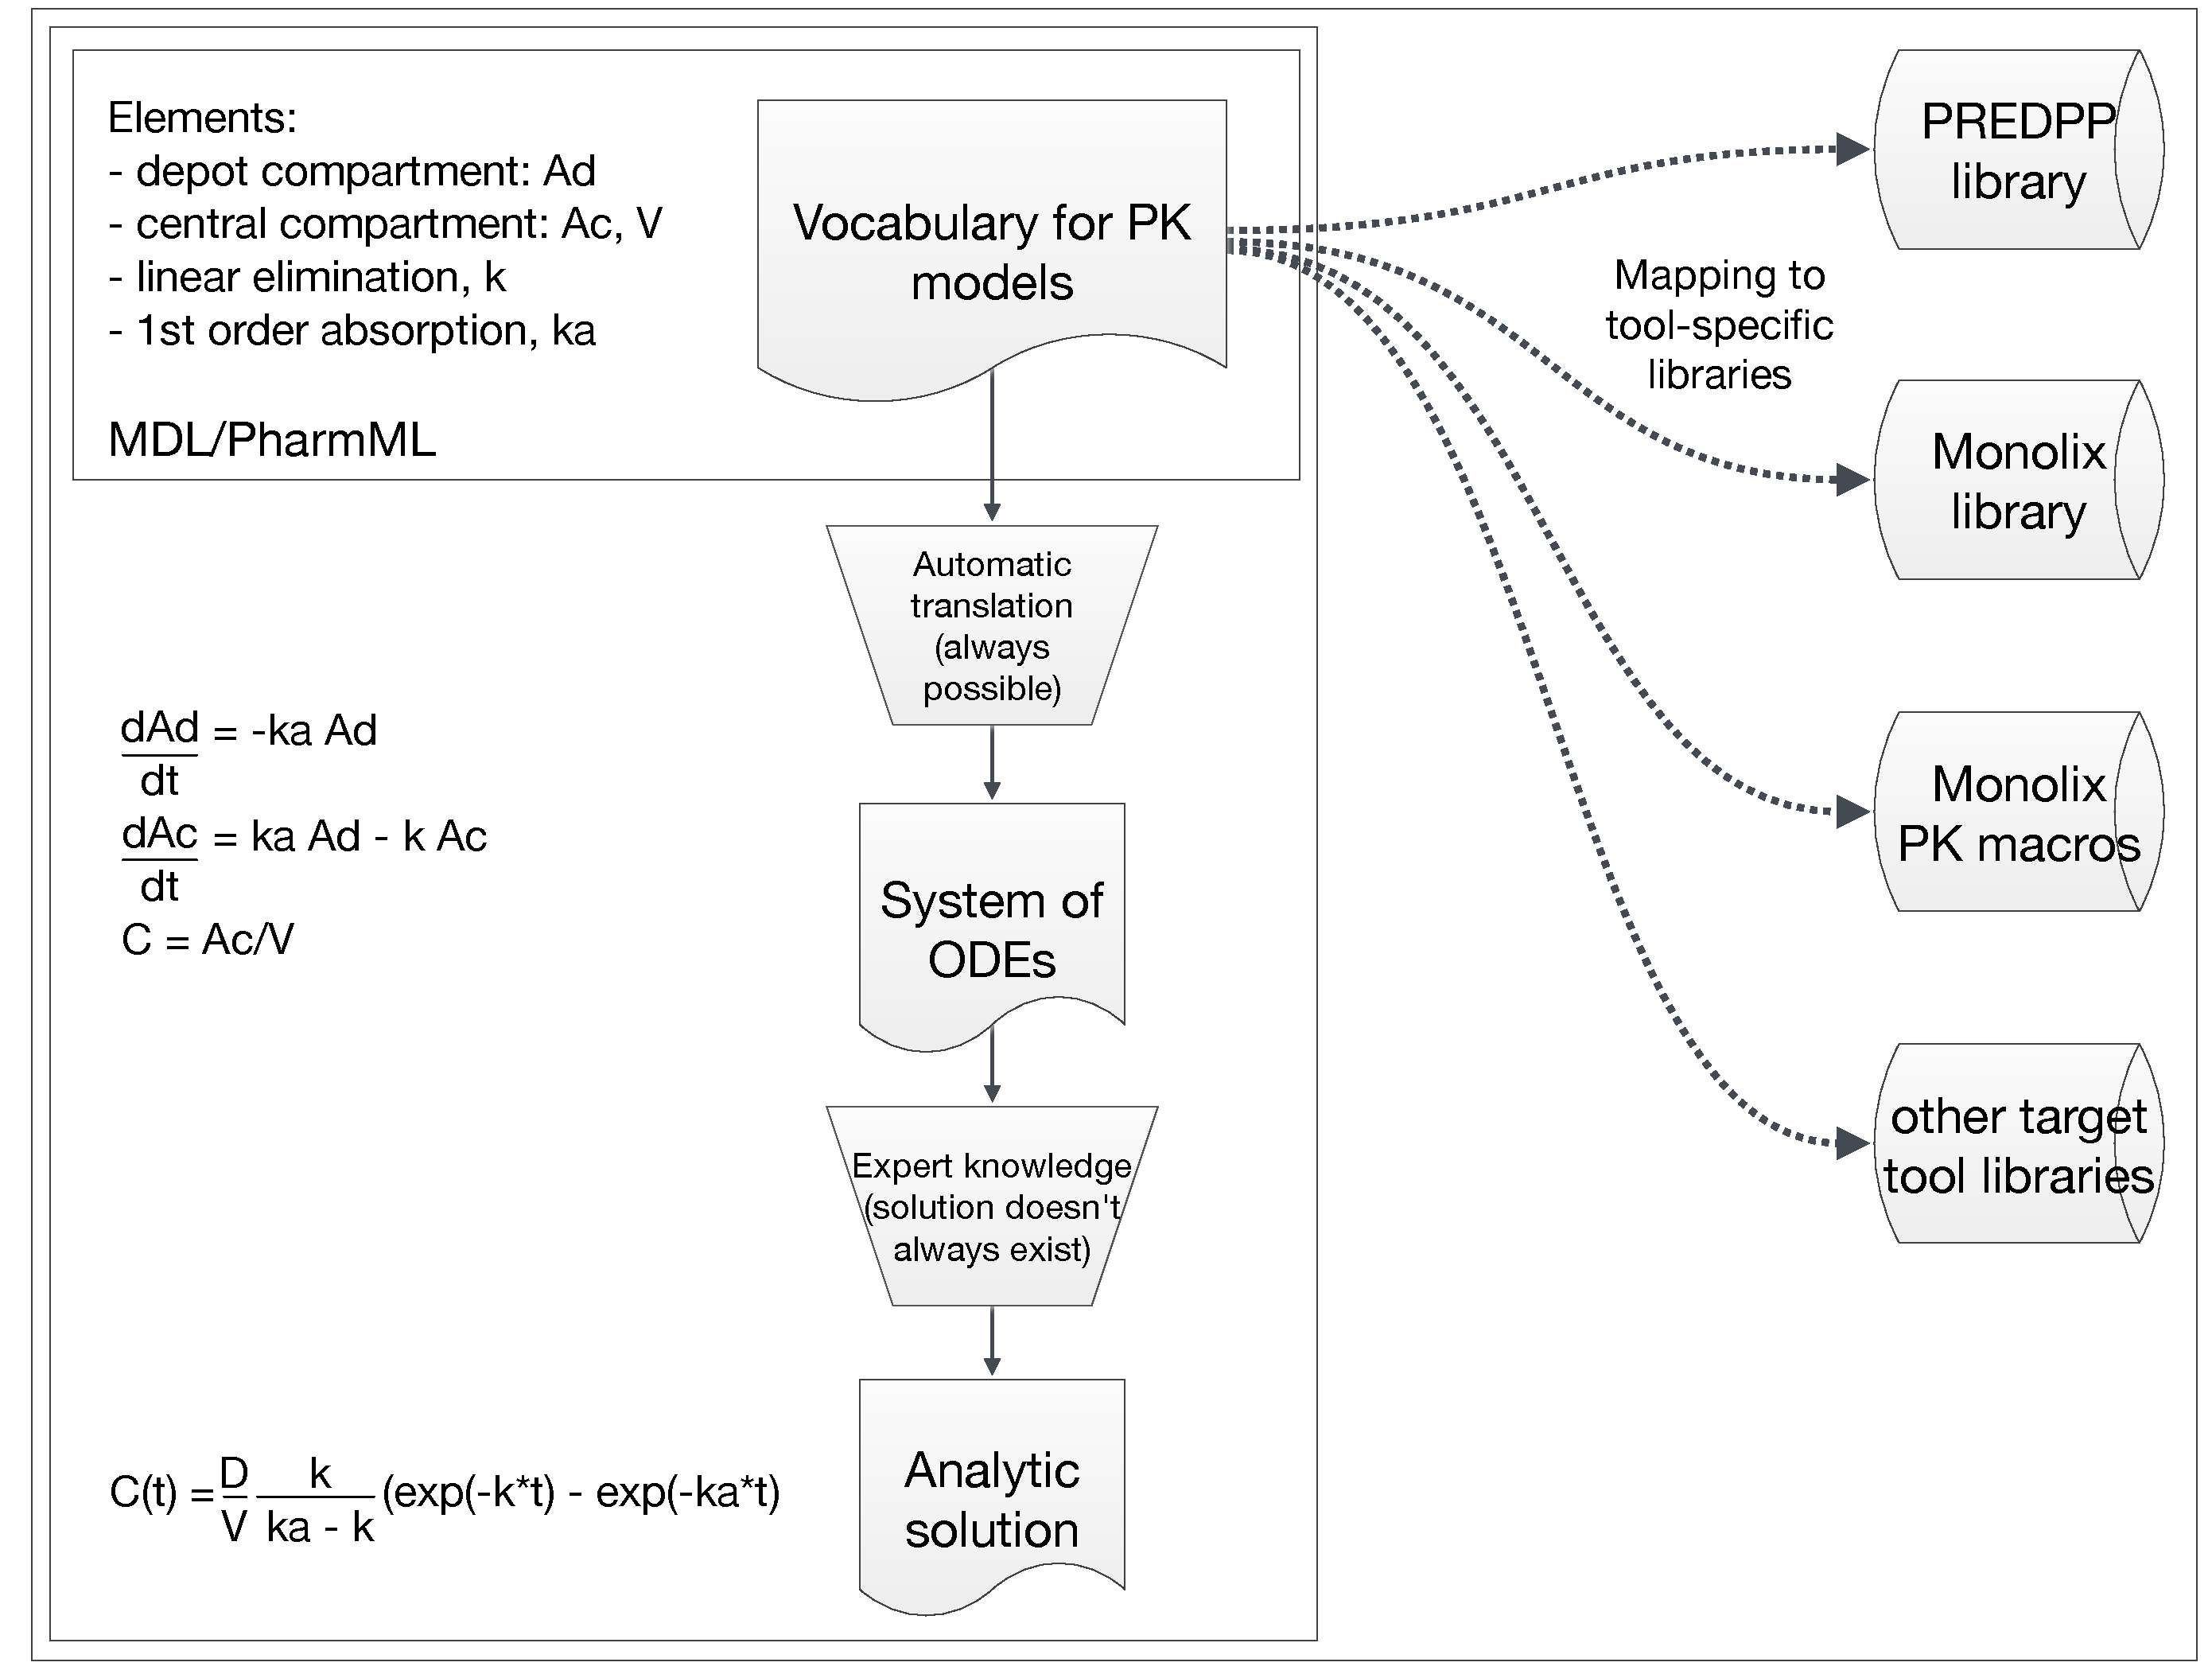
\includegraphics[width=160mm]{pics/PKmacrosPrinciple.pdf}
 \caption{A diagram explaining how the PK macro system can be used in practise. The inner 
 MDL/PharmML box contains the information to be stored in PharmML, i.e. the macros and arguments 
 from the PK model vocabulary. It can then be automatically translated into a set of ODEs and for some 
 models there exists an analytic solution. Models encoded using the controlled vocabulary can be 
 mapped to tool specific implementations (dotted lines).}
 \label{fig:flowDiagram}
\end{figure}
In this case four macros, with one or more arguments, are used to encode a basic \emph{oral 1-compartment 
model with linear elimination} consisting of the following items
\begin{enumerate}
\item
depot compartment, with amount \emph{Ad},
\item
central compartment, with amount \emph{Ac} and volume \emph{V},
\item
oral administration, 1$^{st}$ order absorption with rate constant \emph{ka}, and 
\item
linear elimination, with rate constant \emph{k}.
\end{enumerate}
%For other examples see Tab.\ref{tab:MappingTable}. 
This is the \emph{only} information that needs to be encoded in PharmML for this particular PK model. It 
corresponds to the following macro
\lstset{language=NONMEMdataSet}
\begin{lstlisting}
		compartment(cmt=1,concentration=Cc,volume=V) 
		oral(cmt=1, ka) 
		elimination(cmt=1, k)
\end{lstlisting}
Any information about input, i.e. dosing times and amounts will be stored in the dataset 
or explicitly within the \xelem{TrialDesign}.

The key \marginpar{\HandCuffLeft} realisation is that every set of such macro statements, 
if correctly defined, can be translated automatically into a unique set of ODE's and/or 
algebraic equations, in this case:
\begin{align}
\frac{dAd}{dt} &= -ka \times Ad \nonumber \\
\frac{dAc}{dt} &= ka \times Ad - k \times Ac  \nonumber \\
C &= Ac/V \nonumber
\end{align}

Moreover, for some models such as the above one, there exists an analytic solution. This however cannot 
be derived automatically for an arbitrary ODE system. It requires a powerful symbolic calculation 
software or expert knowledge. Once the PK model macros and their attribute set have been defined, 
a mapping to tool-specific libraries can be provided, see Fig.\ref{fig:flowDiagram}. 
This again requires expert knowledge of each particular tool. 



%%%%%%%%%%%%%%%%%%%%%%%%%%%%%%%%%%%%%%%%%%%%%%%%%%%%%%%%%%%%%%%%%%%%%%%
\section{PK macros in PharmML}
\label{subsec:PKmacros}

\subsection{MLXTRAN macros}
\label{sec:MLXTRANmacros}

PK macros offer an equation-free encoding solution for pharmacokinetic models. 
The novel system allows to implement in MLXTRAN virtually any compartmental 
model within well-defined constraints. See \cite{MLXTRANforMonolix:2014} for a detailed 
description. The following table lists the available PK macros with their arguments. 

\begin{table}[ht!]
\begin{center}
\begin{tabular}{lll}
  \hline
  \hline
Component & Macro & Arguments \\
  \hline
Compartment 			& \textit{compartment}	 	& cmt, amount, volume, concentration \\
Peripheral compartment	& \textit{peripheral}			& \textbf{kij}, \textbf{k$\_$i$\_$j}, amount, volume, concentration \\
Effect compartment 		& \textit{effect} 				& cmt, \textbf{ke0}, concentration \\
Absorption from a depot 	& \textit{depot} 				& type/adm, \textbf{Tlag}, \textbf{p}, target, \textbf{Tk0}, \textbf{ka}, \textbf{Ktr}/\textbf{Mtt} \\
Absorption for IV dose 	& \textit{iv} 				& cmt, type/adm, \textbf{Tlag}, \textbf{p} \\
0-order absorption 		& \textit{absorption}			& cmt, type/adm, \textbf{Tlag}, \textbf{p}, \textbf{Tk0} \\[-.5ex]
					& or \textit{oral}				& \\
1st order absorption 	& \textit{absorption}			& cmt, type/adm, \textbf{Tlag}, \textbf{p}, \textbf{ka}, \textbf{Ktr}/\textbf{Mtt} \\[-.5ex]
					& or \textit{oral}				& \\
Linear elimination 		& \textit{elimination}			& cmt, volume, \textbf{k}, \textbf{CL} \\
MM elimination 		& \textit{elimination}			& cmt, \textbf{Km}, \textbf{Vm} \\
Transfer 				& \textit{transfer}			& from, to, \textbf{kt} \\
  \hline
\end{tabular}
\caption{PK macros and their arguments as used in MLXTRAN, based on 
\cite{MLXTRANforMonolix:2014}. Please, note that there are more components listed, 
10, than macros, 9, actually defined in the MLXTRAN system. Different absorption 
and elimination types are listed separately for better readability. The arguments can be 
devided in two groups. Those who can act alone in the macro are marked with bold font,
all others need to be assigned a numerical value or a symbol reference, see explanation in text.}
\label{tab:MLXPLORElibrary}
\end{center}
\end{table}
One can distinguish two types of arguments, see Table \ref{tab:MLXPLORElibrary}. 
The arguments marked with \textbf{bold} font, can be simply references to identifiers 
defined somewhere else in the model file such as \emph{ka} or \emph{Tlag}. The remaining 
arguments cannot be left unassigned and have to be explicitly specified as attributes 
of the \xelem{Value} element and subsequently assigned a numerical value or 
symbol reference, e.g. \emph{cmt} or \emph{amount}. See Section 
\ref{subsec:encodingRules} for the detailed explanation.

%An essential aspect of the macros is their connectivity to the 
%remaining model elements and the data. The necessary extensions in the current structure are
%discussed, for the input in section \ref{subsec:LinkingMacrosDatasets} and for the output in 
%section \ref{subsec:macroOutputLink}. 

%{\color{red} \scshape{NEW}}
%%%%%%%%%%%%%%%%%%%%%%%%%%%%%%%%%%%%%%%%%%%%%%%%%%%%%%%%%
\subsection{Encoding rules}
\label{subsec:encodingRules}
To provide the full support for MLXTRAN PK macros, all macros and their (unordered) named 
arguments have to be encodable, see Table \ref{tab:MLXPLORElibrary}. Every macro has its own 
PharmML element, e.g. the basic \emph{concentration} macro with all its arguments, encoded as \xelem{Value} 
elements, will be encoded within the \xelem{Concentration} element. The optional attribute \xatt{argument}
is assigned a value corresponding to the argument of the macro. 

%\subparagraph{The basic principle for the implementation and translation to and from PharmML} 
%Macros arguments are encoded as attributes of macro elements only if an assignment is required, 
%otherwise we just refer to them with the standard \xelem{SymbRef} element. 

As mentioned above, there are two types of arguments, and the following rules 
are defined to achieve a consistent macro definition and its interpretation:
\begin{itemize}
\item
\textbf{bold} arguments (\emph{can act alone}) can be references to symbol identifiers defined in other 
places in the model, such as \xatt{k}, \xatt{ka} etc.
\begin{itemize}
\item
cannot be assigned numerical values or expressions within the macro -- 
all such assignments must be defined outside the \xelem{PKmacros} element, for example in the 
\xelem{ParameterModel} or in the \xelem{ModellingSteps} section
\item
if an argument, e.g. 'k', is specified in a macro only, as shown below
\lstset{language=NONMEMdataSet}
\begin{lstlisting}
		elimination(cmt=1, k)
\end{lstlisting}
then a simple \xatt{SymbIdRef} is sufficient
 \lstset{language=XML}
\begin{lstlisting}
                <Elimination>
                    <!-- cmt argument omitted -->>
                    <Value>
                        <ct:SymbRef blkIdRef="pm1" symbIdRef="k"/>
                    </Value>
                </Elimination>
\end{lstlisting}
but it must be defined in a parameter model, here \xatt{pm1}.
\item
if a symbol identifier, here 'k1', is assigned to the key-word argument \xatt{k}, e.g.
\lstset{language=NONMEMdataSet}
\begin{lstlisting}
		elimination(cmt=1, k=k1)
\end{lstlisting}
 then both the keyword as argument, \xatt{k}, and the \xatt{symbIdRef}, \xatt{k1} are required 
 \lstset{language=XML}
\begin{lstlisting}
                <Elimination>
                    <!-- cmt argument omitted -->>
                    <Value argument="k">
                        <ct:SymbRef blkIdRef="pm1" symbIdRef="k1"/>
                    </Value>
                </Elimination>
\end{lstlisting}
\end{itemize}
\item
all \textit{other} arguments (which \emph{cannot act alone}), e.g. 'cmt' or 'amount' as in the following macro
\lstset{language=NONMEMdataSet}
\begin{lstlisting}
		compartment(cmt=1, amount=Ac)
\end{lstlisting}
 \lstset{language=XML}
have to be specified as attributes first and subsequently assigned a numerical value 
or a symbol reference using element \xatt{SymbRef} as in the following code snippet
\begin{lstlisting}
                <Compartment>
                    <Value argument="cmt">
                        <ct:Int>1</ct:Int>
                    </Value>
                    <Value argument="amount">
                        <ct:SymbRef symbIdRef="Ac"/>
                    </Value>
                </Compartment>
\end{lstlisting}

\end{itemize}


%For example, the \emph{elimination} macro defining the linear elimination with rate constant \xatt{k}
%from the first compartment reads
%\lstset{language=NONMEMdataSet}
%\begin{lstlisting}
%		elimination(cmt=1, k)
%		OR
%		elimination(cmt=1, k=k1)		
%		NOT ALLOWED
%		elimination(cmt=1, k = 0.5)		
%\end{lstlisting}
%and is encoded in PharmML as
%\lstset{language=XML}
%\begin{lstlisting}
%            <!-- omitted other model elements-->
%                <Elimination>
%                    <Value argument="cmt">
%                        <ct:Int>1</ct:Int>
%                    </Value>
%                    <Value>
%                        <ct:SymbRef blkIdRef="pm1" symbIdRef="k"/>
%                    </Value>
%                    OR
%                    <Value argument="k">
%                        <ct:SymbRef blkIdRef="pm1" symbIdRef="k1"/>
%                    </Value>
%                </Elimination>
%            </PKmacros>
%        </StructuralModel>
%\end{lstlisting}
%This code makes the above principle and these two implementation options clear. In the first case, 
%an assignment is necessary. The attribute \xatt{argument="cmt"} is used to specify the compartment argument 
%of the macro \xelem{Elimination} and in the next line the number '1' is assigned to it.
%
%In the second case, the elimination rate parameter \xatt{k} is simply referred to without an assignment. 
%The mandatory here \xatt{blkIdRef} attribute points to the parameter model, \xatt{pm1}, where \xatt{k} 
%is expected to be defined.


%%%%%%%%%%%%%%%%%%%%%%%%%%%%%%%%%%%%%%%%%%%%%%%%%%%%%%%%%
\subsection{Fixed argument values and exceptions}
\label{subsec:fixedArguments}
All but one macro have a fixed set of arguments, e.g. the \xatt{compartment} can take only these predefined
four arguments: \xatt{\{cmt, amount, volume, concentration\}}. The exception is the \xatt{peripheral} macro with three fixed
arguments \xatt{\{amount, volume, concentration\}} and a variable one, \xatt{k\_ij or k\_i\_j}, where \xatt{i} and
\xatt{j} stand for input and output compartment, respectively. These compartments numbers are set 
according to the model configuration. 

For example, in the case of models ADVAN11 or 12, see section \ref{subsubsec:ADVAN12} 
for a complete description of the latter, 
we need to set the \xatt{kij} argument names accordingly to the model specification, 
meaning the macro 
\lstset{language=NONMEMdataSet}
\begin{lstlisting}
		peripheral(k12, k21, amount=Ap1)
\end{lstlisting}
will be implemented as shown in the following snippet
\lstset{language=XML}
\begin{lstlisting}
                <Peripheral>
                    <Value>
                        <ct:SymbRef blkIdRef="pm1" symbIdRef="k12"/>
                    </Value>
                    <Value>
                        <ct:SymbRef blkIdRef="pm1" symbIdRef="k21"/>
                    </Value>
                    <!-- omitted amount argument -->
                </Peripheral>
\end{lstlisting}

The \xatt{k\_ij or k\_i\_j} attributes are a special case in that an assignment in the macro 
formulated as
\lstset{language=NONMEMdataSet}
\begin{lstlisting}
		peripheral(k12, k21 = k_test, amount=Ap1)
\end{lstlisting}
will be translated to PharmML as
\lstset{language=XML}
\begin{lstlisting}
                <Peripheral>
                    <Value>
                        <ct:SymbRef blkIdRef="pm1" symbIdRef="k12"/>
                    </Value>
                    <Value argument="k21">
                        <ct:SymbRef blkIdRef="pm1" symbIdRef="k_test"/>
                    </Value>
                    <!-- omitted amount argument -->
                </Peripheral>
\end{lstlisting}
Note the difference between the implementation of the two first arguments. 
The first argument, \xatt{k12}, is implemented as before because no assignment
is required. In the second case we use the \xatt{argument} attribute to inform 
the target tool about the meaning of the assigned parameter. Therefore, the 
symbol \xatt{k12} is not a parameter itself and \xatt{k\_test} serves as the 
transfer parameter \xatt{kij} between compartment 1 and 2, which can be defined 
in the parameter model \xatt{pm1} and can be assigned any value in the 
\xelem{ModellingSteps} section.


%\newpage
%%%%%%%%%%%%%%%%%%%%%%%%%%%%%%%%%%%%%%%%%%%%%%%%%%%%%%%%%
\subsection{Macros and target tools}
\label{subsec:LinkingMacrosDatasets}

One of the main reasons to introduce the system of macros is that they offer a flexible 
and efficient way of encoding PK models. The proposed macros are fully compatible with 
Monolix and its data format, see Appendix B in \cite{Monolix4.3.2UserGuide:2014}. 

Of course, from the perspective of the interoperability platform \marginpar{\HandCuffLeft}
it is crucial that the models stored in PharmML using macros can be unambiguously translated 
to NONMEM and other target tools. Especially the compatibility with the predefined PREDPP 
routines (i.e. ADVAN 1-4 and 10-12) is essential because of their popularity among the 
NONMEM modellers community. 

To understand the required translation rules, the knowledge of relevant NONMEM and 
MONOLIX features and the dataset formats these target tools use is helpful. 
For convenience, the most essential differences between these tools/formats from the 
perspective of the macros and their usage are listed here
\begin{itemize}
\item
In PREDPP (but only when using ADVAN 1-4, 10-12 routines) the \emph{DEPOT} 
compartment is always considered as the $1^{st}$ compartment, the central compartment 
as $2^{nd}$ and the peripheral compartments as $3^{rd}$, $4^{th}$ etc. 
\item
In contrast, MONOLIX doesn't assign a number to the \emph{DEPOT} 
compartment at all and the numbering starts usually with the central compartment. 
\item
The CMT column, standard in NONMEM dataset, is not used in Monolix. It uses an ADM 
column instead.
\end{itemize}

%To provide such flexibility we have to 
%ensure that they can handle, for start, the three basic data formats 
%\begin{itemize}
%\item
%NONMEM dataset, as described in \cite{NONMEM:2009} (with restrictions such as 
%no support for PREDPP keywords and special encoding tricks)
%\item
%MONOLIX' version, a modified NONMEM dataset, see a detailed specification in \cite{Monolix4.3.2UserGuide:2014}.
%\item
%\xelem{TrialDesign} model provides the possibility to store data records in a tool-independent manner. 
%\xelem{IndividualDosing} element is the place where relevant dosing data can be encoded inline
%or be referred to from an external datafile. The actual mapping is defined within the \xelem{Activity}
%tag.  
%\end{itemize}
%There are many incompatible differences between these dataset formats, \marginpar{\HandCuffLeft} 
%here just a couple relevant points from the point of view of the PK macros


%Due to the lack of an common data format and in order to make sure that the macros can work 
%both with Monolix, NONMEM and \xelem{TrialDesing} coded datasets we needed a modification 
%in the original MLXTRAN macros.
%
%\begin{figure}[ht!]
%\centering
% 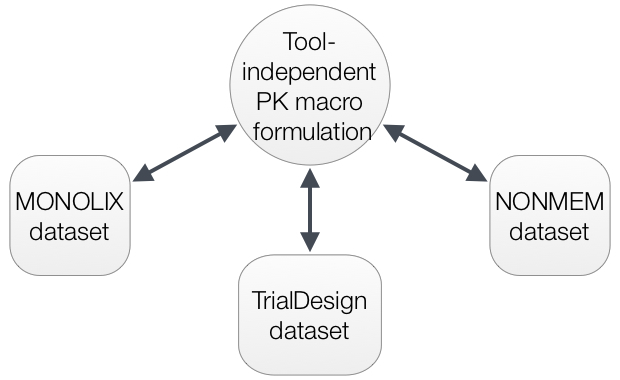
\includegraphics[width=0.6\textwidth]{pics/MacrosDatasets}
%\caption{Macros are suppose to work with Monolix, NONMEM and \xelem{TrialDesing} coded 
%datasets. }
%\label{fig:MacrosDatasets}
%\end{figure}

%\subsubsection{Modifications}
%Figure \ref{fig:ComplexModel3A} and Table \ref{tab:datasetComparison} will be used 
%to illustrate the problem. Two administrations are defined, one oral, one intravenous.
%While MONOLIX (left) doesn't assign a number to the depot compartment, 
%NONMEM (right) does. The differences are inter-connected with the format of the dataset 
%compatible with each model version. Monolix uses administration type number stored 
%in the ADM column to identify the administration process. NONMEM requires a CMT 
%column in the dataset to link a drug administration with its target. 
%
%To describe an oral administration in the original MONOLIX macro system two lines 
%of code are required and is sufficient to inform the tool about the dosing process
%\lstset{language=NONMEMdataSet}
%\begin{lstlisting}
%		compartment(cmt=1, volume=V, concentration=Cc)
%		oral(adm=1, cmt=1, ka)
%\end{lstlisting}
%
%
%However, to make the macro work with the NONMEM dataset, 
%Figure \ref{tab:datasetComparison} (RIGHT), the following modifications (in red) 
%are required
%\lstset{language=NONMEMdataSet}
%\begin{lstlisting}
%		compartment(cmt=1, volume=V, concentration=Cc)
%		[*compartment(cmt=2, amount=Depot)*]
%		oral(adm=1, [*fromCmt=2,*] cmt=1,k)
%\end{lstlisting} 
%A new \xatt{compartment} macro for the depot needs to be defined and to make 
%the connection with the target compartment work a new attribute \xatt{fromCmt}
%has to be introduced.

\subsubsection{An illustrative example}
Figure \ref{fig:ComplexModel_Rules} and datasets in Table \ref{tab:C3ModelData} 
give us some clues about two alternative interpretations for a model with at 
least one oral administration, dependent on the target tool. Note, that apart from a
few predefined models, such as ADVAN1-4 and 10-12, one can assign an arbitrary 
number to the  (first) depot compartment in the NONMEM dataset. This is exactly what 
happens in this example. While in MONOLIX we would have only two compartments 
with assigned number to them, all four compartments have numbers assigned in NONMEM,
Figure \ref{fig:ComplexModel_Rules} (right). This means that when translating a model 
from PharmML, a transformation of the associated dataset is required. 

It is therefore possible to translate a macro and dataset, utilising the ADM column to identify 
administrations, used by Monolix into an PREDPP/ADVAN based NONMEM encoding 
system with data set using the CMT column, see Figure \ref{fig:ComplexModel_Rules} and
Table \ref{tab:C3ModelData}.


\begin{figure}[h!]
\centering
 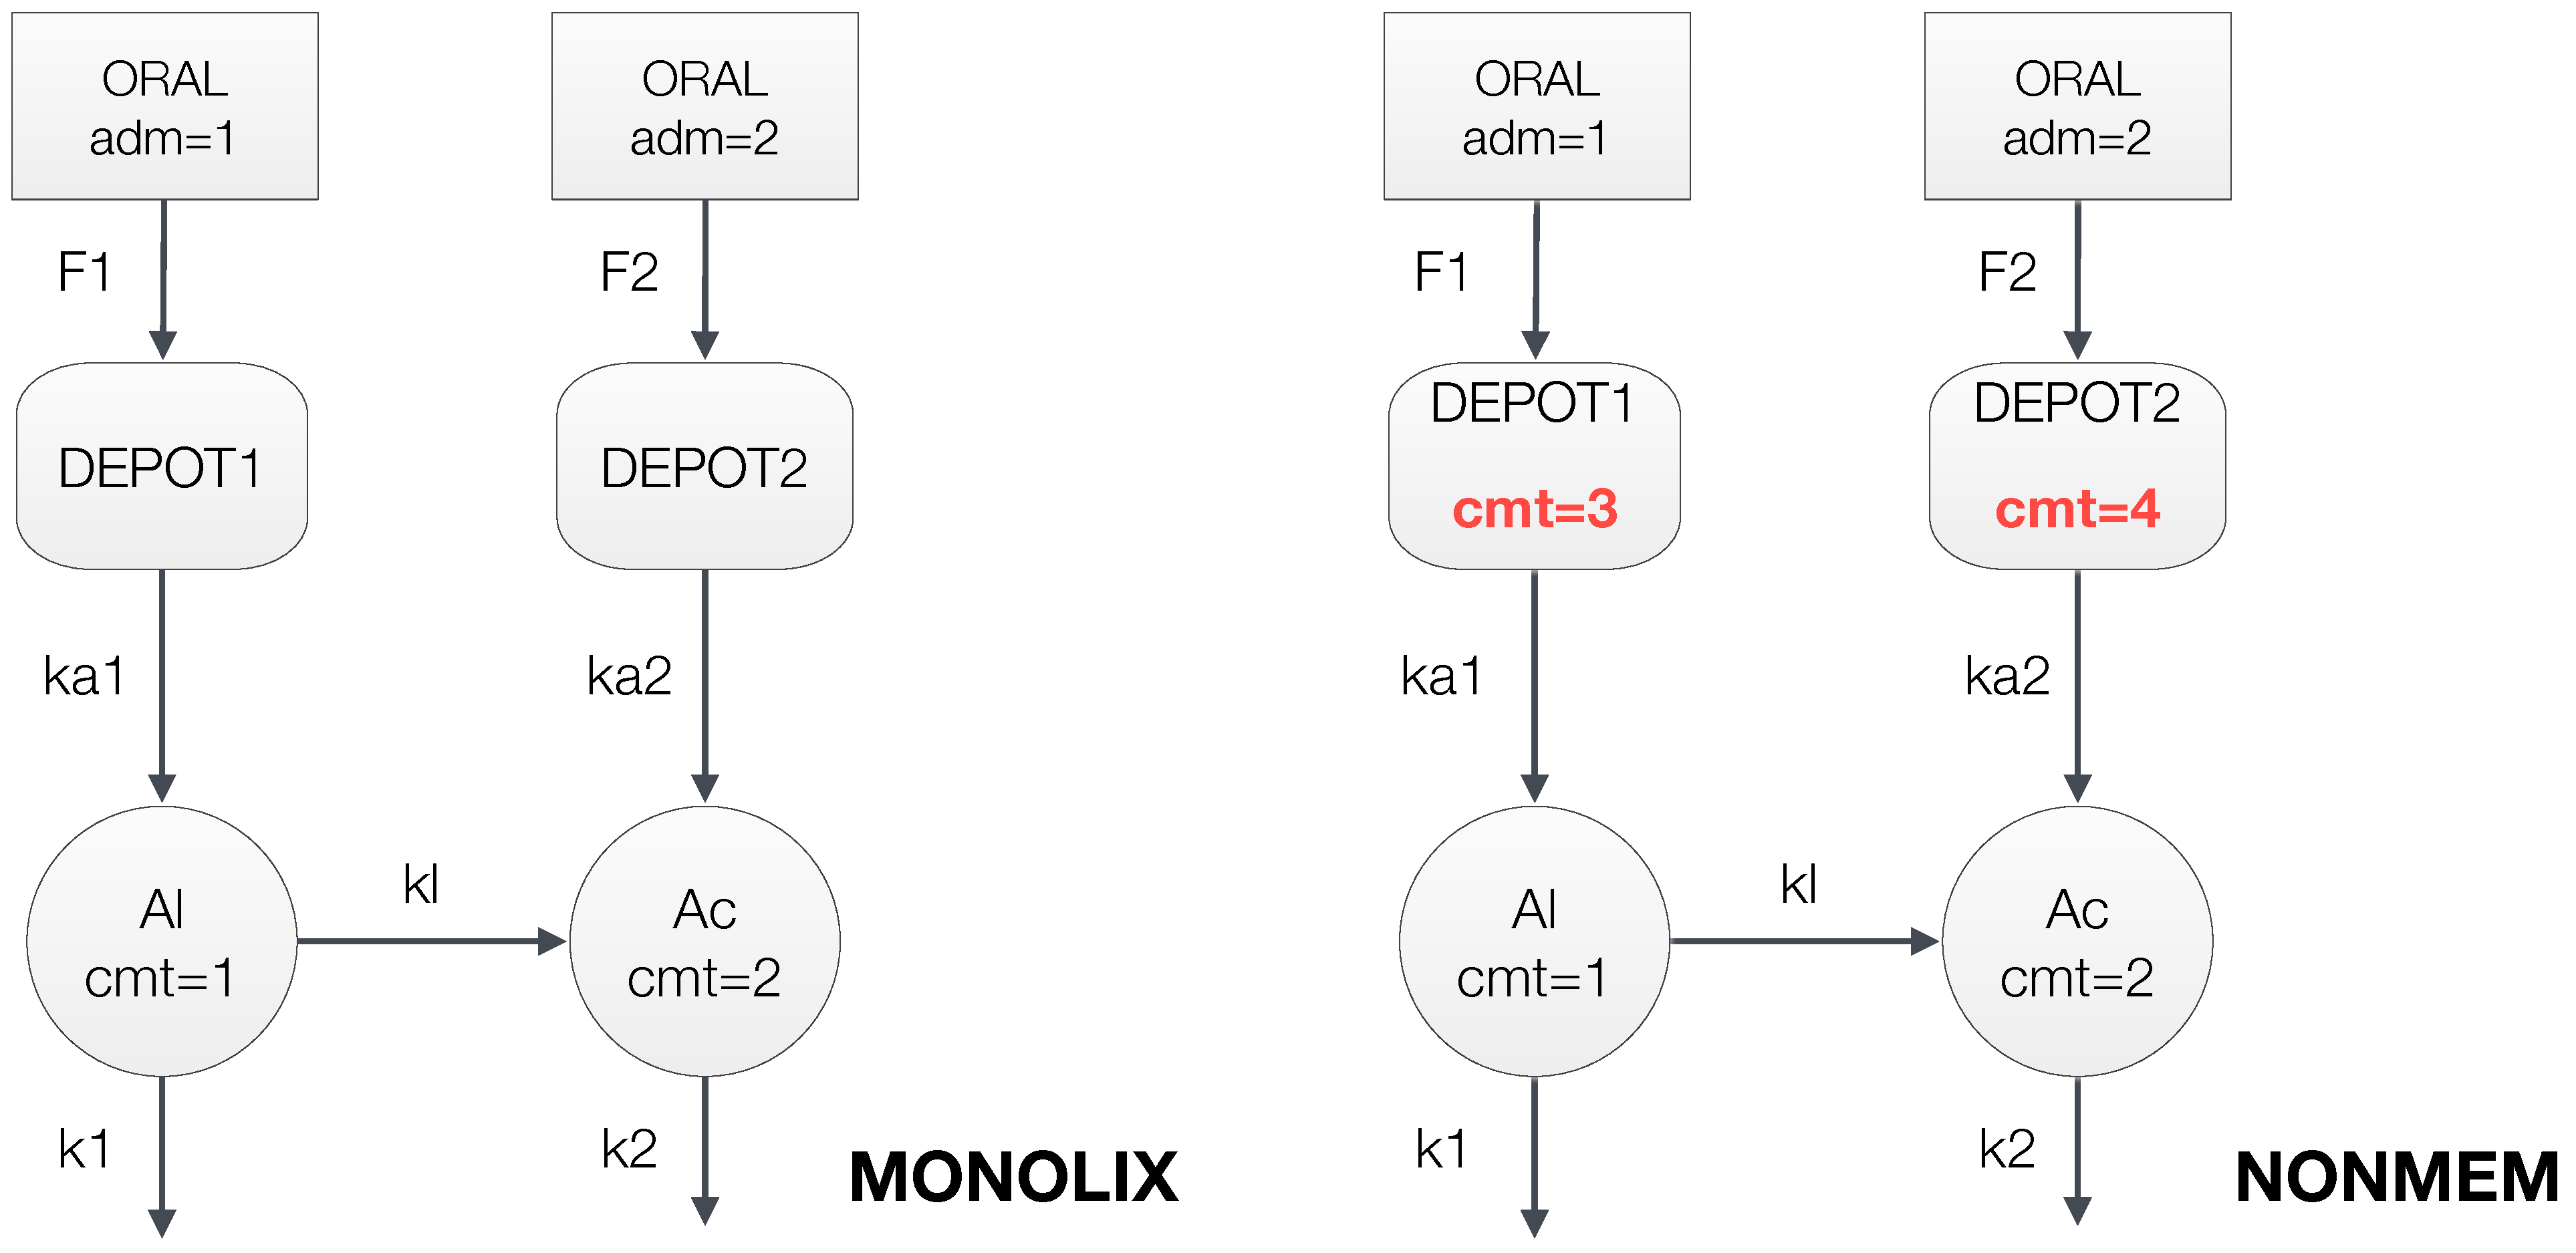
\includegraphics[width=140mm]{pics/ComplexModel_Rules.pdf}
\caption{Two interpretations for a model with two oral administrations.
While MONOLIX (left) doesn't assign a number to the depot compartments, 
NONMEM (right) does. The translation of macro coded models to target tools 
requires in this case changes in the dataset as well, see Table \ref{tab:C3ModelData}.}
\label{fig:ComplexModel_Rules}
\end{figure}



\begin{table}[h!]
\footnotesize
\parbox{.5\linewidth}{
\centering
\begin{tabular}{ccccc}
  \hline
   \multicolumn{5}{c}{\textbf{MONOLIX}} \\
  \hline
ID	& TIME  & AMT	 & \textbf{ADM}  &	Y \\
  \hline
1	& 6	    & 10	& \textbf{1}	 & . \\
1	& 9	    & 20	& \textbf{2}	 & . \\
1	& 18	    & 10	& \textbf{1}	 & . \\
1	& 33	    & 20	& \textbf{2}	 & . \\
...     &  ...     &  ...     &  ...  & ... \\
1	& 0	    & .	& .	& 0 \\
1	& 12	    & .	& .	& 1.18 \\
...     &  ...     &  ...     & ...  & ...\\
\end{tabular}
}
\hfill
\parbox{.5\linewidth}{
\centering
\begin{tabular}{ccccc}
  \hline
   \multicolumn{5}{c}{\textbf{NONMEM}} \\
  \hline
ID	& TIME  & AMT	 & \textbf{\textcolor{red}{CMT}} &	DV \\
  \hline
1	& 6	    & 10	& \textbf{\textcolor{red}{3}}	 & . \\
1	& 9	    & 20	& \textbf{\textcolor{red}{4}}	 & . \\
1	& 18	    & 10	& \textbf{\textcolor{red}{3}}	 & . \\
1	& 33	    & 20	& \textbf{\textcolor{red}{4}}	 & . \\
...     &  ...     &  ...     &  ...  & ... \\
1	& 0	    & .	& 1	& 0 \\
1	& 12	    & .	& 1	& 1.18 \\
...     &  ...     &  ...     & ...  & ...\\
\end{tabular}
}
\caption{MONOLIX and NONMEM datasets for the model above, Figure 
\ref{fig:ComplexModel_Rules}. The translator has to make sure that the numbers 
in the ADM column of the former are properly converted to the CMT column in the latter dataset.}
\label{tab:C3ModelData}
\end{table}
%See Appendix \ref{sec:PKMacrosAppendix} for more examples.

\subsubsection{Basic translation rules}
The following few basic translation rules should be treated merely as a guidance
because they do not cover the whole aspect of the model/data handling within the 
interoperability platform but are limited to the models encoded with macros. 
A more careful analysis is required to cover the structural model exchange between 
the key target tools and associated datasets.

The flow of the data within the framework \marginpar{\HandCuffLeft}  has been so far 
successfully avoided/neglected and needs to return to the agenda again. 

\subparagraph{A -- Models corresponding to ADVAN 1-4 and 10-12}
Fortunately, the translation of models encoded with macros and having their equivalents 
in routines ADVAN1-4 and 10-12 in PREDPP and their datasets is straightforward. 
Simply, one has to translate a corresponding macro into its equivalent ADVAN 
routine and then to rename the ADM column in the MONOLIX data set into CMT, 
see for more details and examples in Section \ref{subsec:PREDPPinMACROS}
and \ref{subsec:PREDPPinMACROSExamples}.

\subparagraph{B -- All other models}
For every oral administration one new depot compartment needs to be introduced
and assigned a number. The Figure \ref{fig:ComplexModel_Rules} and datasets 
in Table \ref{tab:C3ModelData} can again help to understand what is required. 

In this example, \xatt{adm=1} and \xatt{adm=2} denote two oral administrations. 
In the NONMEM system, Figure \ref{fig:ComplexModel_Rules} (right), '1' and '2' are  
assigned to the central and peripheral compartment respectively, as in the MONOLIX 
case, so that the next free numbers, '3' and '4', will be assigned to the depot 
compartments. 

Next, the NONMEM dataset needs to be produced based on the information stored 
in the MONOLIX dataset in such a way that it will match the new compartment 
numbering scheme with the CMT column replacing the ADM column. 

The oral administration, \xatt{adm=1}, aims now at the compartment 3, so that '1' 
in the ADM column will correspond to '3' in the CMT column. Similarly, \xatt{adm=2}, 
aims now at the compartment 4, so that '2' in the ADM column will be translated to '4' 
in the CMT column.

As additional rules, applicable for all models, one should keep in mind that 
(1) Y column in a MONOLIX dataset has to be renamed into DV of the NONMEM dataset 
and (2) the TINF column has to be renamed into RATE 
and its content recalculated accordingly. 

%\subparagraph{Column names} TINF and Y columns in the original datasets have 
%to be renamed to RATE and DV, respectively. 

%\begin{figure}[h!]
%\centering
% 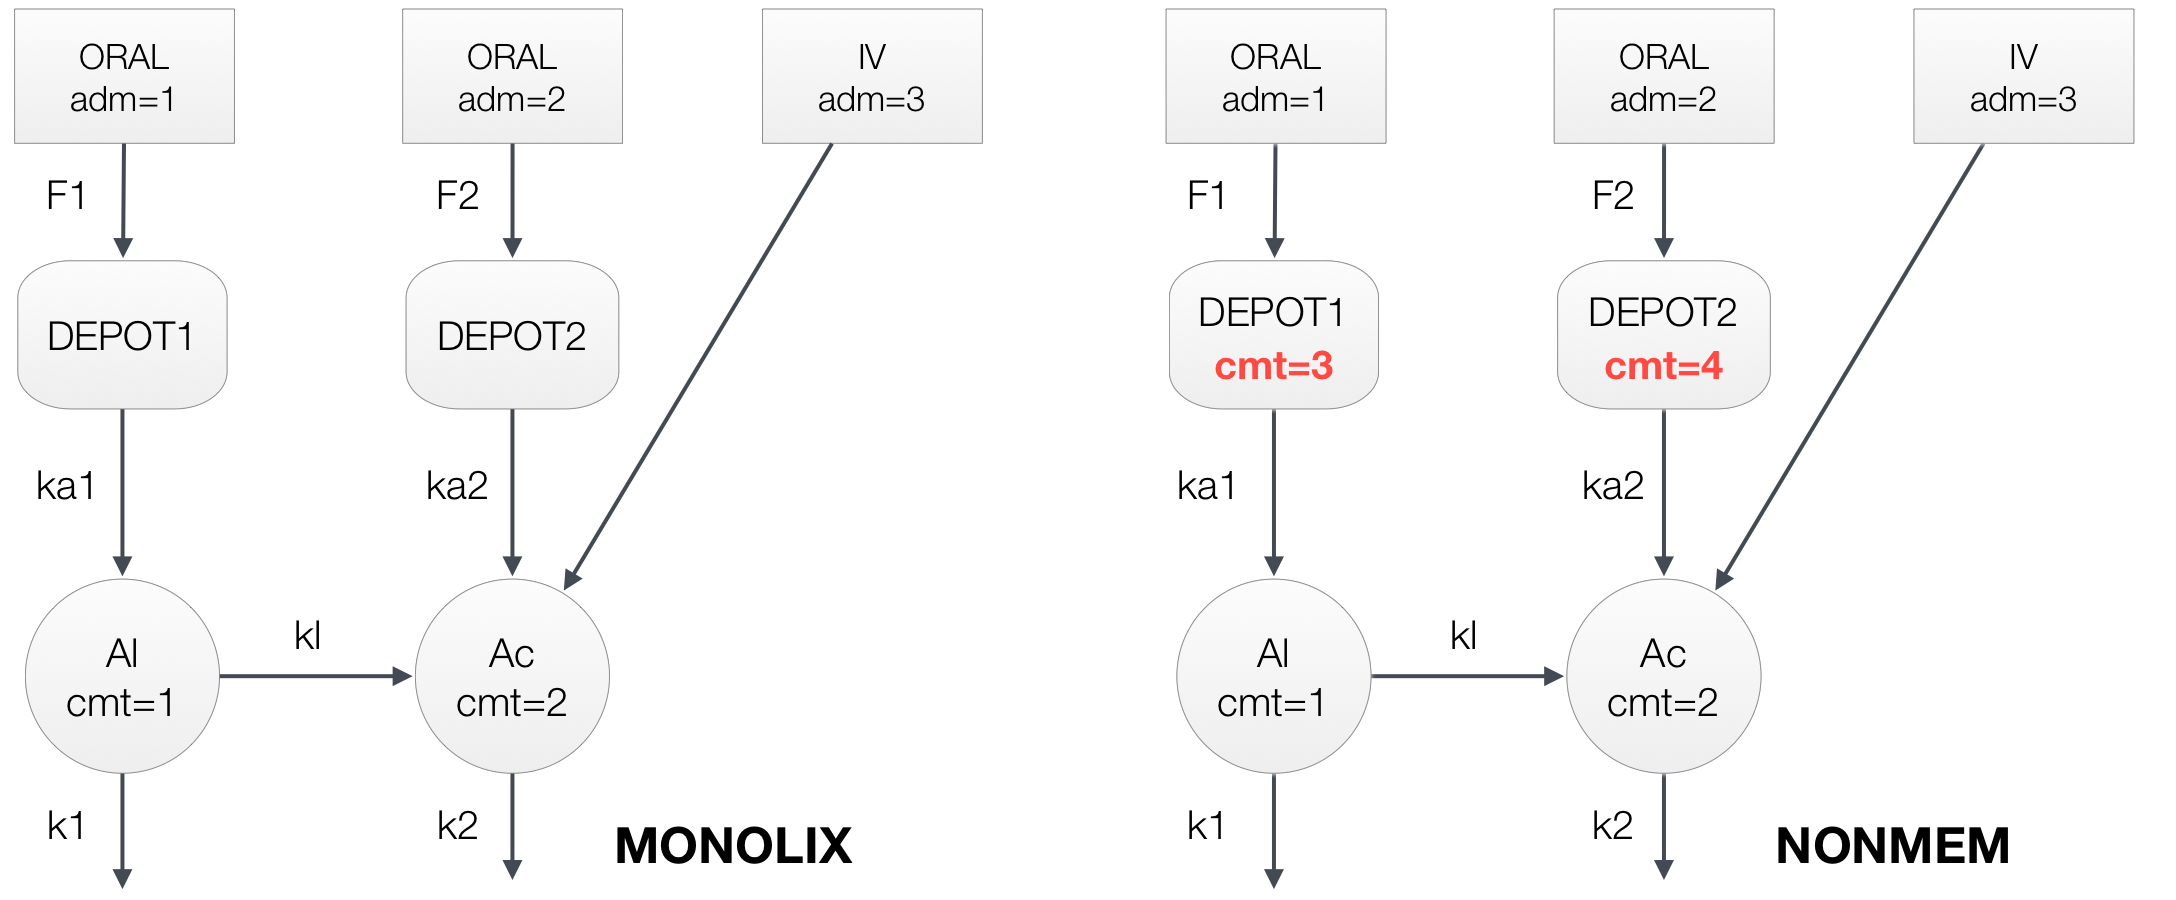
\includegraphics[width=120mm]{pics/ComplexModel3}
%\caption{Two model interpretations for a model with more then one administration 
%from which at least one is of oral type, dependent on the target tool. 
%While MONOLIX (left) doesn't assign a number to the depot compartment, 
%NONMEM (right) does. The difference is inter-connected with the format of the 
%dataset compatible with each model version, see Table \ref{tab:datasetComparison}.}
%\label{fig:ComplexModel3A}
%\end{figure}
%
%
%\begin{table}[ht!]
%\footnotesize
%\parbox{.5\linewidth}{
%\centering
%\begin{tabular}{ccccc}
%  \hline
%     \multicolumn{5}{c}{\textbf{MONOLIX}} \\
%  \hline
%ID	& TIME  & AMT	 & \textbf{ADM} &	Y \\
%  \hline
%1	& 0	    & 2.24	& \textbf{2}	& . \\
%1	& 1	    & .	& .		 	& 142 \\
%1	& 2	    & .	& .	 		& 54.9 \\
%1	& 3	    & .	& .			& 25.9 \\
%1	& 4	    & .	& .			& 17.5 \\
%1	& 6	    & 7	& \textbf{1}	& . \\
%1	& 7	    & .	& .			& 192 \\
%1	& 8	    & .	& .			& 141 \\
%1	& 9	    & .	& .			& 189 \\
%2	& 0	    & 2.73	& \textbf{2}	& . \\
%2	& 1	    & . 	& .			& 176 \\
%...     &  ...     &  ...     & ...  			& ...\\
%\end{tabular}
%}
%\hfill
%\parbox{.5\linewidth}{
%\centering
%\begin{tabular}{ccccc}
%  \hline
%   \multicolumn{5}{c}{\textbf{NONMEM}} \\
%  \hline
%ID	& TIME  & AMT	 & \textbf{\textcolor{red}{CMT}} &	Y \\
%  \hline
%1	& 0	    & 2.24	& \textbf{\textcolor{red}{1}}	& . \\
%1	& 1	    & .	& .		 	& 142 \\
%1	& 2	    & .	& .	 		& 54.9 \\
%1	& 3	    & .	& .			& 25.9 \\
%1	& 4	    & .	& .			& 17.5 \\
%1	& 6	    & 7	& \textbf{\textcolor{red}{2}}	& . \\
%1	& 7	    & .	& .			& 192 \\
%1	& 8	    & .	& .			& 141 \\
%1	& 9	    & .	& .			& 189 \\
%2	& 0	    & 2.73	& \textbf{\textcolor{red}{1}}	& . \\
%2	& 1	    & . 	& .	 		& 176 \\
%...     &  ...     &  ...     & ...  			& ...\\
%\end{tabular}
%}
%\caption{Comparison of NONMEM and MONOLIX datasets for the model shown 
%in Figure \ref{fig:ComplexModel3A}. NONMEM requires additionally a CMT column in 
%the dataset, whereas MONOLIX doesn't and uses instead administration type number
%stored in the ADM column.}
%\label{tab:datasetComparison}
%\end{table}


%\newpage
\subsubsection{Datasets mapping}
We will discuss now briefly the mapping between macros and the MONOLIX dataset, 
i.e. the mapping between \xatt{adm/type} attributes in the PK macros and the 
administration type as stored in the ADM column,
\begin{itemize}
\item 
\xelem{TargetMapping} element with the \xatt{blkIdRef} attribute, the latter one because 
in PharmML multiple structural models are allowed, so we have to specify which model is 
holding the target compartment definition
\item
\xelem{Map} element with
\begin{itemize}
\item 
\xatt{dataSymbol} -- attribute denoting the target symbol as encoded in a dataset and
\item 
new attribute \xatt{admNumber} -- to identify the target symbol in the model.
\end{itemize}
\end{itemize}

%\xatt{modelSymbol}/\xatt{cmtNumber}/

The use of these new elements is explained in the Table \ref{tab:mappingNONMEMAndMacros}. 
%(Left) the mapping if MONOLIX dataset is used, {right} for the NONMEM dat set.
\begin{table}[ht!]
\setlength{\tabcolsep}{5pt}
\begin{center}
\begin{tabular}{l}
  \hline
  \hline
MONOLIX datasets mapping \\ %  	& NONMEM datasets mapping \\
  \hline
\lstset{language=XML}
\begin{lstlisting}
<ExternalDataSet toolName="Monolix" oid="MLXoid">
    <!-- omitted details -->
    
    <ColumnMapping>
        <ds:ColumnRef columnIdRef="ADM"/>
        <ds:TargetMapping blkIdRef="sm3">
            <ds:Map dataSymbol="1" admNumber="1"/>
            <ds:Map dataSymbol="2" admNumber="2"/>
            <ds:Map dataSymbol="3" admNumber="3"/>
        </ds:TargetMapping>
    </ColumnMapping>
    
    <!-- omitted ColumnMappings and Definition of dataset  
    		columns such as ID,TIME,AMT,ADM  -->
\end{lstlisting}
%&
%\lstset{language=XML}
%\begin{lstlisting}
%<NONMEMdataSet oid="NMoid">
%    <!-- omitted details -->
%    
%    <ColumnMapping>
%        <ds:ColumnRef columnIdRef="CMT"/>
%        <ds:TargetMapping blkIdRef="sm3">
%            <ds:Map dataSymbol="2" cmtNumber="2"/>
%            <ds:Map dataSymbol="3" cmtNumber="3"/>
%            <ds:Map dataSymbol="4" cmtNumber="4"/>
%        </ds:TargetMapping>
%    </ColumnMapping>
%    
%    <!-- omitted Definition of dataset  
%    	columns such as ID,TIME,AMT,CMT  -->
%\end{lstlisting}
%\\
%& OR \\
%&
%\lstset{language=XML}
%\begin{lstlisting}
%<NONMEMdataSet oid="NMoid">
%    <!-- omitted details -->
%    
%    <ColumnMapping>
%        <ds:ColumnRef columnIdRef="CMT"/>
%        <ds:TargetMapping blkIdRef="sm3">
%            <ds:Map dataSymbol="2" modelSymbol="Ac"/>
%            <ds:Map dataSymbol="3" modelSymbol="Depot1"/>
%            <ds:Map dataSymbol="4" modelSymbol="Depot2"/>
%        </ds:TargetMapping>
%    </ColumnMapping>
%    
%    <!-- omitted Definition of dataset  
%    	columns such as ID,TIME,AMT,CMT  -->
%\end{lstlisting}
\\
    \hline
\end{tabular}
\caption{Mappings of MONOLIX type datasets and PK macros.}
\label{tab:mappingNONMEMAndMacros}
\end{center}
\end{table}



%\newpage
%%%%%%%%%%%%%%%%%%%%%%%%%%%%%%%%%%%%%%%%%%%%%%%%%%%%%%%%%
\subsection{Linking macros and \xelem{TrialDesign}}
\label{subsec:LinkingMacrosTrialDesign}
\xelem{TrialDesign} section provides an alternative to encode design and to store 
data records (observations, dosing and covariates) in a tool-independent manner. 
The \xelem{IndividualDosing} element is the place where relevant dosing data can 
be encoded inline or be referred to from an external datafile. The actual mapping 
is defined within the \xelem{Activity} tag.

A minor extension in the \xelem{TrialDesign} is necessary to link the administrations coded
in \xelem{Activity} elements  to the targets in the PK macros and identified using the 
\xatt{adm} attribute, i.e.
\begin{itemize}
\item
new value \textit{administrationType} is added to the \xatt{inputTarget} attribute.
\end{itemize}
Otherwise, elements defined in the last section will be reused. The Table 
\ref{tab:mappingTrialDesignAndMacros} shows the implementations within the 
\xelem{TrialDesign} element in cases when (left) a PK model is expressed using 
algebraic equation with dose parameter, D, and (right) when using PK macros.
\begin{table}[ht!]
\setlength{\tabcolsep}{5pt}
\begin{center}
\begin{tabular}{ll}
  \hline
  \hline
Using dose \xatt{parameter}, D, and algebraic & Using value \emph{administrationType} for \xatt{inputTarget}  \\
equation for PK model, e.g. $C(t)=f(D,V,k,...)$ 	& and \xelem{TargetMapping}/\xelem{Map} elements   \\
(available in PharmML since version 0.2.1)	& 	\\
  \hline
\lstset{language=XML}
\begin{lstlisting}
<Activity oid="actBolusD">
    <Bolus>
        <DoseAmount inputTarget="parameter">
            <ct:SymbRef blkIdRef="sm3" symbIdRef="D"/>
            <ct:Assign>
                <ct:Real>10</ct:Real>
            </ct:Assign>
        </DoseAmount>
        <DosingTimes>
            <!-- e.g. 10 -->
        </DosingTimes>
    </Bolus>
</Activity>
\end{lstlisting}
&
\lstset{language=XML}
\begin{lstlisting}
<Activity oid="actBolusMacro">
    <Bolus>
        <DoseAmount inputTarget="admType">
            <ds:TargetMapping blkIdRef="sm3">
                <ds:Map admNumber="2"/>
            </ds:TargetMapping>
            <ct:Assign>
                <ct:Real>10</ct:Real>
            </ct:Assign>
        </DoseAmount>
        <!-- omitted DosingTimes -->
    </Bolus>
</Activity>
\end{lstlisting}
\\
    \hline
\end{tabular}
\caption{Comparison of the link between administration definitions and structural model, 
dependent on the formulation of the latter. (left) PK model expressed using algebraic equations
 with dose parameter, $D$, and when using the PK macros (right).}
\label{tab:mappingTrialDesignAndMacros}
\end{center}
\end{table}


%{\color{red} \scshape{NEW}}
%\newpage
%%%%%%%%%%%%%%%%%%%%%%%%%%%%%%%%%%%%%%%%%%%%%%%%%%%%%%%%%
\subsection{Connection between macros and the model}
\label{subsec:macroOutputLink}
The possible outputs of PK macros are amounts, e.g. $Ac$, and concentrations, e.g. $C$. 
A PK model defined by a system of macros will often be connected to a subsequent PD 
model, which expects the concentration, $C$, as one of the inputs. Another option is that the output
of the PK macros will be mapped directly to the data in the \xelem{ObservationModel}. 

For the \emph{compartment} macro in question, there are two possibilities, either
\begin{itemize}
\item
the concentration is defined in the macro
\lstset{language=NONMEMdataSet}
\begin{lstlisting}
		compartment(cmt=1,concentration=C, volume=V)
\end{lstlisting}
in which case no output has to be defined explicitly, or
\item
the alternative form of this macro is used
\lstset{language=NONMEMdataSet}
\begin{lstlisting}
		compartment(cmt=1,amount=Ac, volume=V)
\end{lstlisting}
and because eventually the concentration is required, a subsequent assignment for $C$ must be provided in MLXTRAN
in the \emph{EQUATION} block, i.e.
\lstset{language=NONMEMdataSet}
\begin{lstlisting}
		C = Ac/V
\end{lstlisting}
\end{itemize}
In PharmML, these two cases have to be treated accordingly. 
\begin{itemize}
\item
In the first case only the concentration variable, $C$, needs to be defined
\lstset{language=XML}
\begin{lstlisting}
        <StructuralModel blkId="sm1">
            <ct:Variable symbolType="real" symbId="C"/>
            
            <PKmacros>
                    <!-- omitted details of the macro 
                    compartment(cmt=1,concentration=C, volume=V) -->
\end{lstlisting}
\item
in the second case, both the amount variable, $Ac$, and concentration variable, $C$, 
with the $C=Ac/V$ assignment needs to be defined
\lstset{language=XML}
\begin{lstlisting}
        <StructuralModel blkId="sm1">
            <ct:Variable symbolType="real" symbId="Ac"/>
            <ct:Variable symbolType="real" symbId="Cc">
                <ct:Assign>
                    <math:Equation>
                        <math:Binop op="divide">
                            <ct:SymbRef symbIdRef="Ac"/>
                            <ct:SymbRef blkIdRef="pm1" symbIdRef="V"/>
                        </math:Binop>
                    </math:Equation>
                </ct:Assign>
            </ct:Variable>
            
            <PKmacros>
                <Compartment>
                    <!-- omitted details of the macro 
                    compartment(cmt=1,amount=Ac, volume=V) -->
\end{lstlisting}
\end{itemize}
If a model using the PK macros is defined properly, following the principles described above, 
both options make sure that the connection to a subsequent model or the \xelem{ObservationModel} 
can be established.



%%%%%%%%%%%%%%%%%%%%%%%%%%%%%%%%%%%%%%%%%%%%%%%%%%%%%%%%%%%%%%%%%%%%%%
\section{PREDPP models and PK macros}
\label{subsec:PREDPPinMACROS}

This section describes PREDPP library models as encoded in routines ADVAN1-4 and 10-12 
and their PK macros implementation. 


As explained in Section \ref{subsec:LinkingMacrosDatasets} there are differences between 
NONMEM and MONOLIX and their datasets one has to consider when dealing with PK macros.
They manifest themselves also in that way how the transfer rate constants are numbered/named. 
Models with more then two compartments and with 1st order input (using \emph{DEPOT} 
compartment) will have different transfer rate symbols, e.g.:
\begin{itemize}
\item
ADVAN 4
\begin{table}[ht]
\begin{center}
\begin{tabular}{lcc}
  \hline
  \hline
				 	& PREDPP routines 	& PK macros \\
  \hline
transfer rate constants 	& k23, k32 		& k12, k21  \\
   \hline
\end{tabular}
\end{center}
\end{table}

\item
ADVAN 12 
\begin{table}[ht]
\begin{center}
\begin{tabular}{lcc}
  \hline
  \hline
				 	& PREDPP routines 	& PK macros \\
  \hline
transfer rate constants 	& k23, k32 		& k12, k21  \\
					& k24, k42 		& k13, k31  \\
   \hline
\end{tabular}
\end{center}
\end{table}
\end{itemize}
Models described in this section use the MLXTRAN numbering convention in order to comply
with the PK macros notation.

To allow for a lossless translation between PREDPP coded models and PK macros one needs
to establish well defined translation rules. To achieve this goal and provide help to other 
translation/converter teams one needs to analyse the predefined PREDPP routines ADVAN1-4 \& 10-12
and more specifically to
\begin{enumerate}
\item
understand what they mean
\item
dissect the routines into elementary components and finally 
\item
find equivalent formulation for each such element in the PK macro speak.
\end{enumerate}
The above steps are illustrated in Table \ref{tab:ADVAN_translation} in an abbreviated form. 
In the column \emph{Interpretation} first two steps are implemented, 
the last column provides the according PK macro formulation.

\begin{center}
\begin{longtable}{lll}
  \hline
  \hline
ADVAN routine & Interpretation & MLXTRAN macro \\
\& default TRANS1 &		& \\
%ADVAN\_X & Interpretation & Elements & MLXTRAN macro \\
%(w. TRANS1)		&			 &		    &	\\
\hline
\multicolumn{3}{c}{one compartment}  \\[.1ex]
\hline
%1-comp, IV input
\lstset{language=NONMEMdataSet}
\begin{lstlisting}
ADVAN1
compartment
\end{lstlisting}
&
\lstset{language=Elements}
\begin{lstlisting}
- 1 compartment

- iv bolus administration

- linear elimination
\end{lstlisting}
& 
\lstset{language=MLXTRANcode}
\begin{lstlisting}
compartment(cmt=1, amount=Ac, volume=V)

iv(adm=1, cmt=1)

elimination(cmt=1, k)
\end{lstlisting} 

\\
& 
\\
\hdashline


%1-comp, 1st order input
\lstset{language=NONMEMdataSet}
\begin{lstlisting}
ADVAN2
\end{lstlisting}
&
\lstset{language=Elements}
\begin{lstlisting}
- 1 compartment

- oral administration, 1st order absorption

- linear elimination
\end{lstlisting}
%&
%
&
\lstset{language=MLXTRANcode}
\begin{lstlisting}
compartment(cmt=1, amount=Ac, volume=V)

oral(adm=1, cmt=1, ka)

elimination(cmt=1, k)
\end{lstlisting}

\\
& 
\\
\hdashline

%1-comp, IV input 
%with saturable elimination
\lstset{language=NONMEMdataSet}
\begin{lstlisting}
ADVAN10
\end{lstlisting}
&
\lstset{language=Elements}
\begin{lstlisting}
- 1 compartment

- iv bolus administration

- saturable elimination
\end{lstlisting}
%&
%
&
\lstset{language=MLXTRANcode}
\begin{lstlisting}
compartment(cmt=1, amount=Ac, volume=V)

iv(adm=1, cmt=1)

elimination(cmt=1, Km, Vm)
\end{lstlisting}

\\
\hline
\multicolumn{3}{c}{two compartments}  \\[.1ex]

  \hline

%2-comp, IV input
\lstset{language=NONMEMdataSet}
\begin{lstlisting}
ADVAN3 
\end{lstlisting}
&
\lstset{language=Elements}
\begin{lstlisting}
- 2 compartments 
one central (1) & one peripheral with
linear transfer rates

- iv bolus administration (into 1)

- linear elimination (from 1)
\end{lstlisting}
%&
%
&
\lstset{language=MLXTRANcode}
\begin{lstlisting}
compartment(cmt=1, amount=Ac, volume=V)
peripheral(k12, k21, amount=Ap)


iv(adm=1, cmt=1)

elimination(cmt=1, k)
\end{lstlisting}

\\
& 
\\
\hdashline


%2-comp, 1st order input 
\lstset{language=NONMEMdataSet}
\begin{lstlisting}
ADVAN4 
\end{lstlisting}
&
\lstset{language=Elements}
\begin{lstlisting}
- 2 compartments 
one central (1) & one peripheral with
linear transfer rates

- oral administration, 1st order absorption 
(into 1)

- linear elimination (from 1)
\end{lstlisting}
%&
%
&
\lstset{language=MLXTRANcode}
\begin{lstlisting}
compartment(cmt=1, amount=Ac, volume=V)
peripheral(k12, k21, amount=Ap)


oral(adm=1, cmt=1, ka)

elimination(cmt=1, k)
\end{lstlisting}

\\
\hline
\multicolumn{3}{c}{three compartments}  \\[.1ex]
  \hline
  
%3-comp, IV input 
\lstset{language=NONMEMdataSet}
\begin{lstlisting}
ADVAN11
\end{lstlisting}
&
\lstset{language=Elements}
\begin{lstlisting}
- 3 compartments 
one central (1) & two peripheral with
linear transfer rates

- iv bolus administration (into 1)

- linear elimination (from 1)
\end{lstlisting}
%&
%
&
\lstset{language=MLXTRANcode}
\begin{lstlisting}
compartment(cmt=1, amount=Ac, volume=V)
peripheral(k12, k21, amount=Ap1)
peripheral(k13, k31, amount=Ap2)

iv(adm=1, cmt=1)

elimination(cmt=1, k)
\end{lstlisting}

\\
& 
\\
\hdashline

%3-comp, 1st order input 
\lstset{language=NONMEMdataSet}
\begin{lstlisting}
ADVAN12
\end{lstlisting}
&
\lstset{language=Elements}
\begin{lstlisting}
- 3 compartments 
one central (1) & two peripheral with
linear transfer rates

- oral administration, 1st order absorption 
(into 1)

- linear elimination (from 1)
\end{lstlisting}
%&
%
&
\lstset{language=MLXTRANcode}
\begin{lstlisting}
compartment(cmt=1, amount=Ac, volume=V)
peripheral(k12, k21, amount=Ap1)
peripheral(k13, k31, amount=Ap2)

oral(adm=1, cmt=1, ka)

elimination(cmt=1, k)
\end{lstlisting}
    \\ [+1ex]
      \hline
      \\
\caption{Interpretation and translation of PREDPP models using ADVAN1-4 \& 10-12 routines, 
with default TRANS1 parameterization, into PK macros.}
\label{tab:ADVAN_translation}
\end{longtable}
\end{center}

\begin{figure}[htbp!]
\centering
 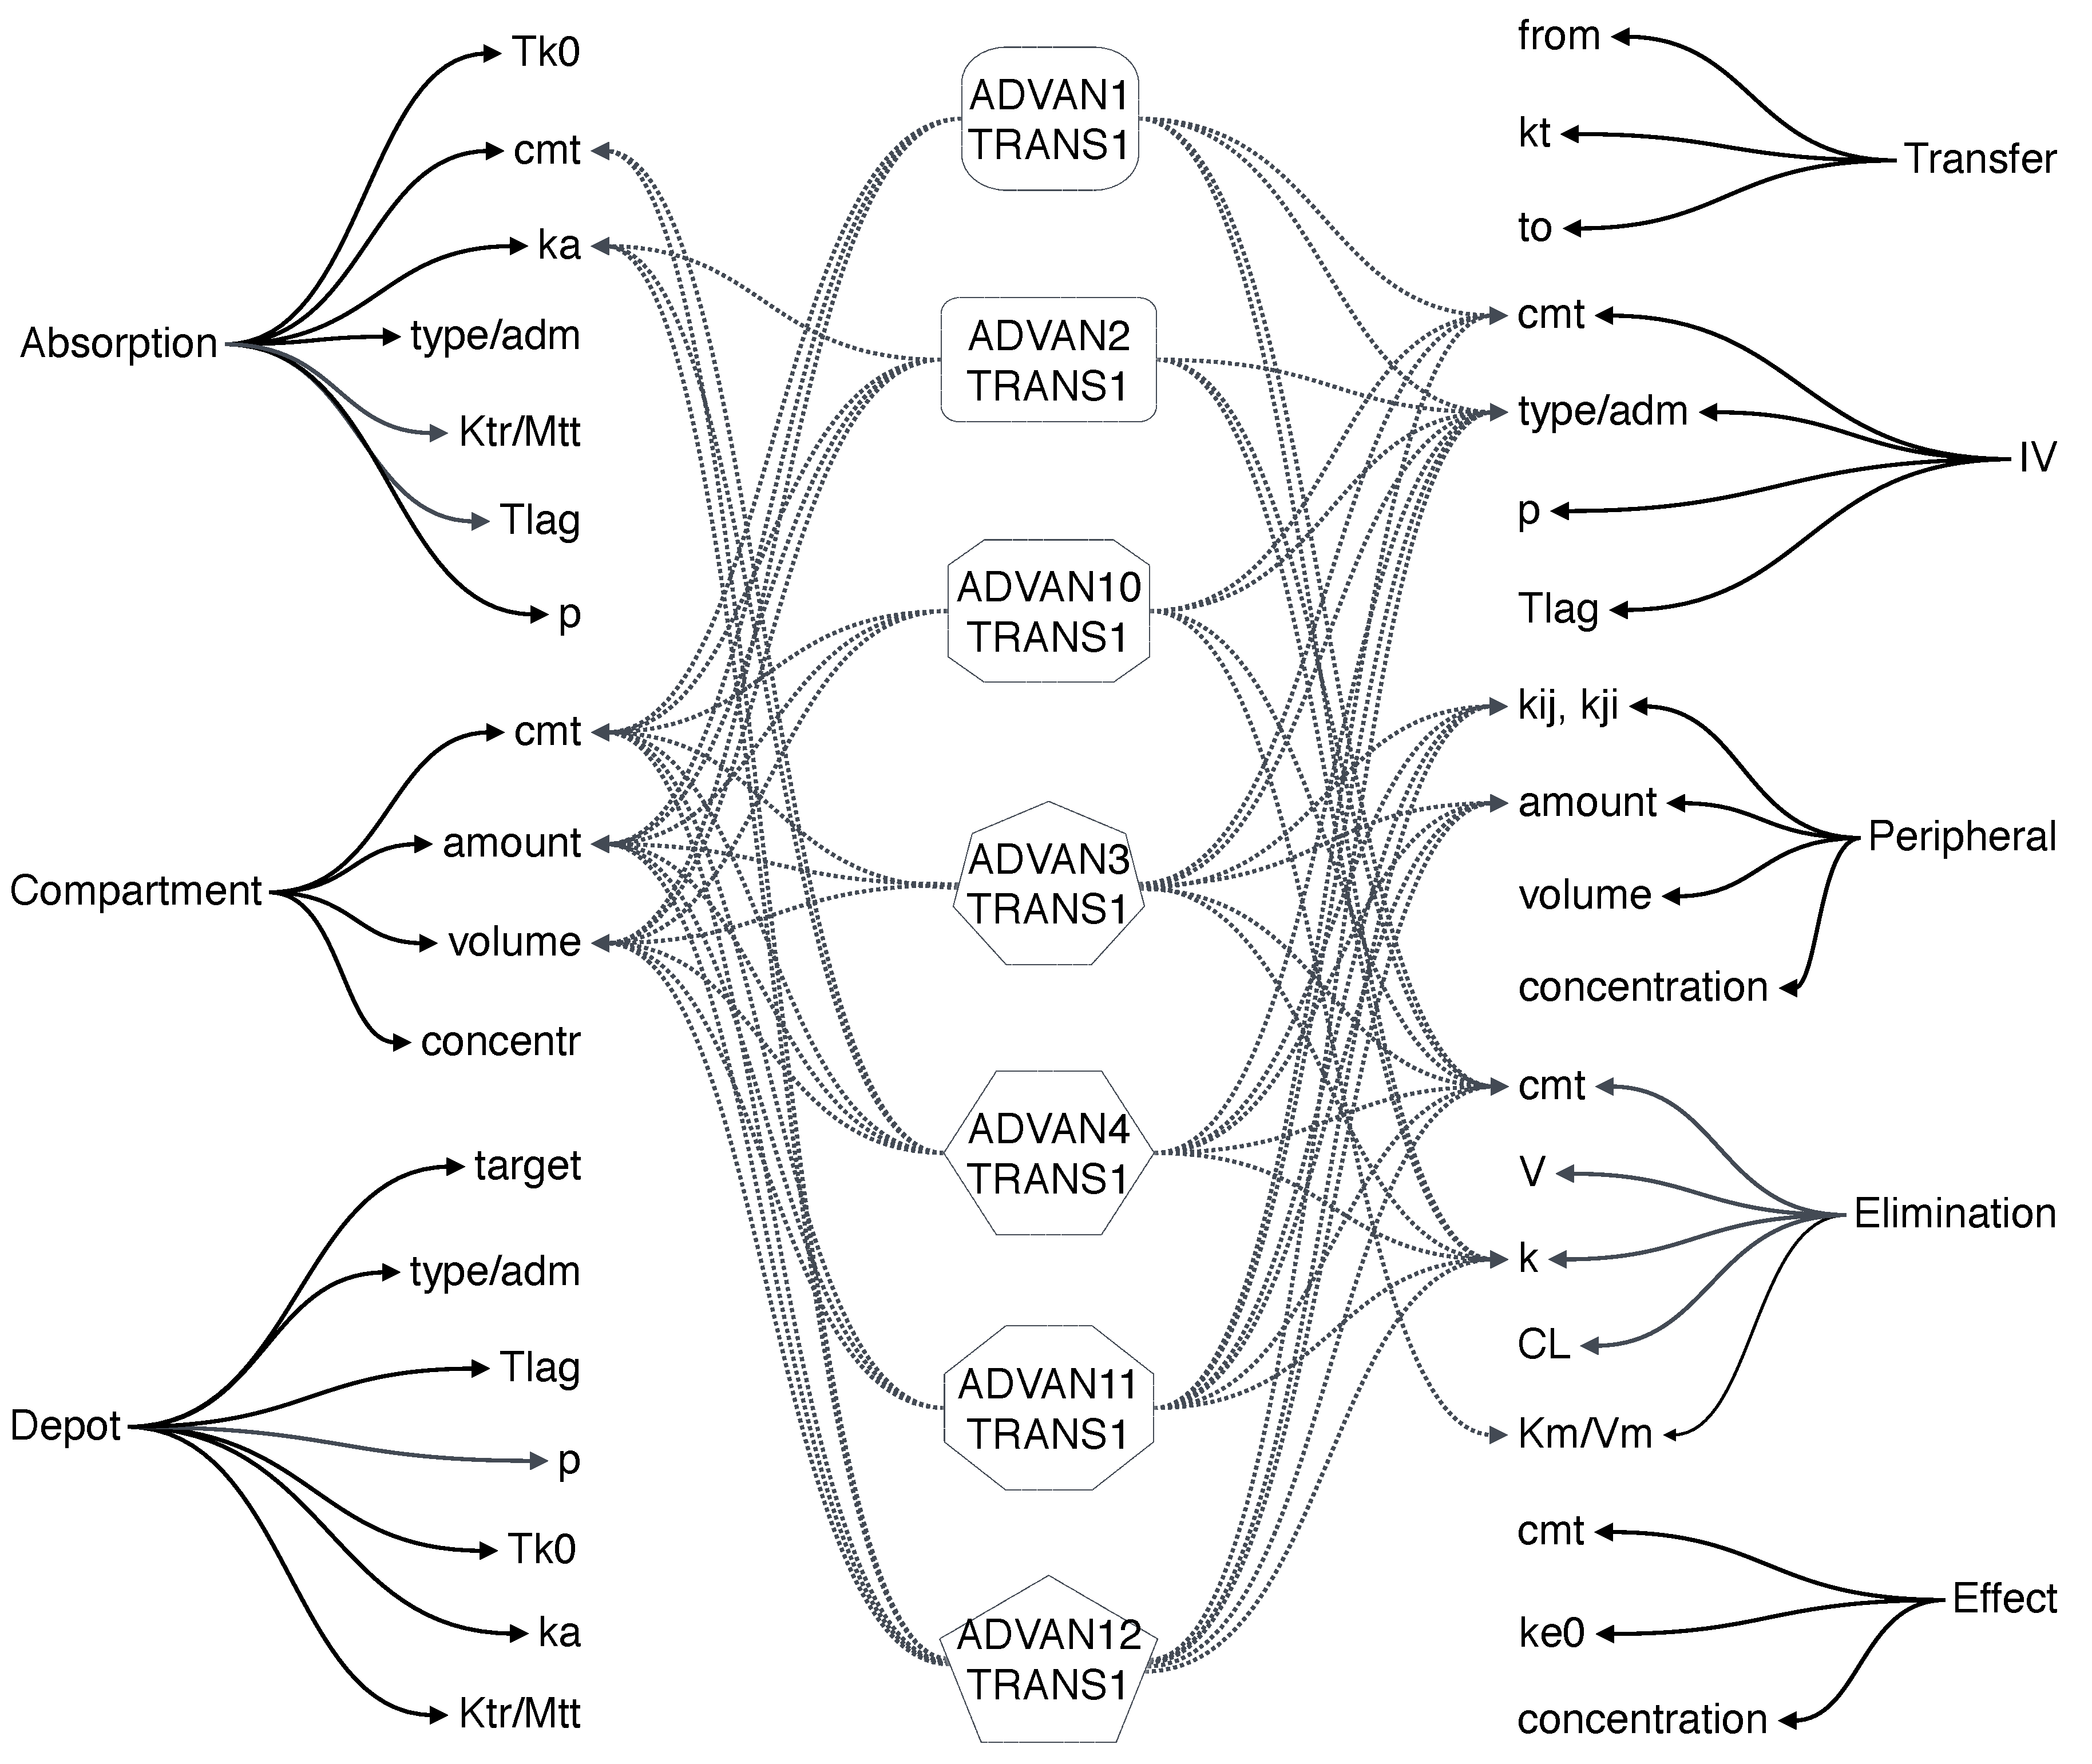
\includegraphics[width=170mm]{pics/AdvanMacrosMaster.pdf}
\caption{The overview of the ADVAN models, with their default parameterisation TRANS1, 
and their connection to PK macros based on the analysis in Table \ref{tab:ADVAN_translation}. 
Each ADVAN model can be uniquely mapped to macros and their attributes. For more 
details see next section with examples.}
\label{fig:AdvanMacrosMaster}
\end{figure}


%%%%%%%%%%%%%%%%%%%%%%%%%%%%%%%%%%%%%%%%%%%%%%%%%%%%%%%%%%%%%%%%%%%%%%
\section{Examples}
\label{subsec:PREDPPinMACROSExamples}

We will conclude this section with two examples of PREDPP coded models 
and show their implementation in PK macros in PharmML, which will
illustrate number of aspects described in the previous sections such as 
interpretation of the models, their translation and the associated dataset 
conversion.

%%%%%%%%%%%%%%%%%%%%%%%%%%%%%%%%%%%%%%%%%%%%%%%%%%%%%%%%%%%%%%%%%%%%%%
\subsection{ADVAN4, TRANS1 -- 2-comp 1st order input}
ODE formulation:
\begin{align}
\frac{dAd}{dt} &= -ka \times Ad \nonumber \\
\frac{dAc}{dt} &= ka \times Ad - k_{12} \times Ac + k_{21} \times Ap - k \times Ac  \nonumber \\
\frac{dAp}{dt} &= k_{12} \times Ac - k_{21} \times Ap  \nonumber
\end{align}

\begin{figure}[htbp!]
\centering
 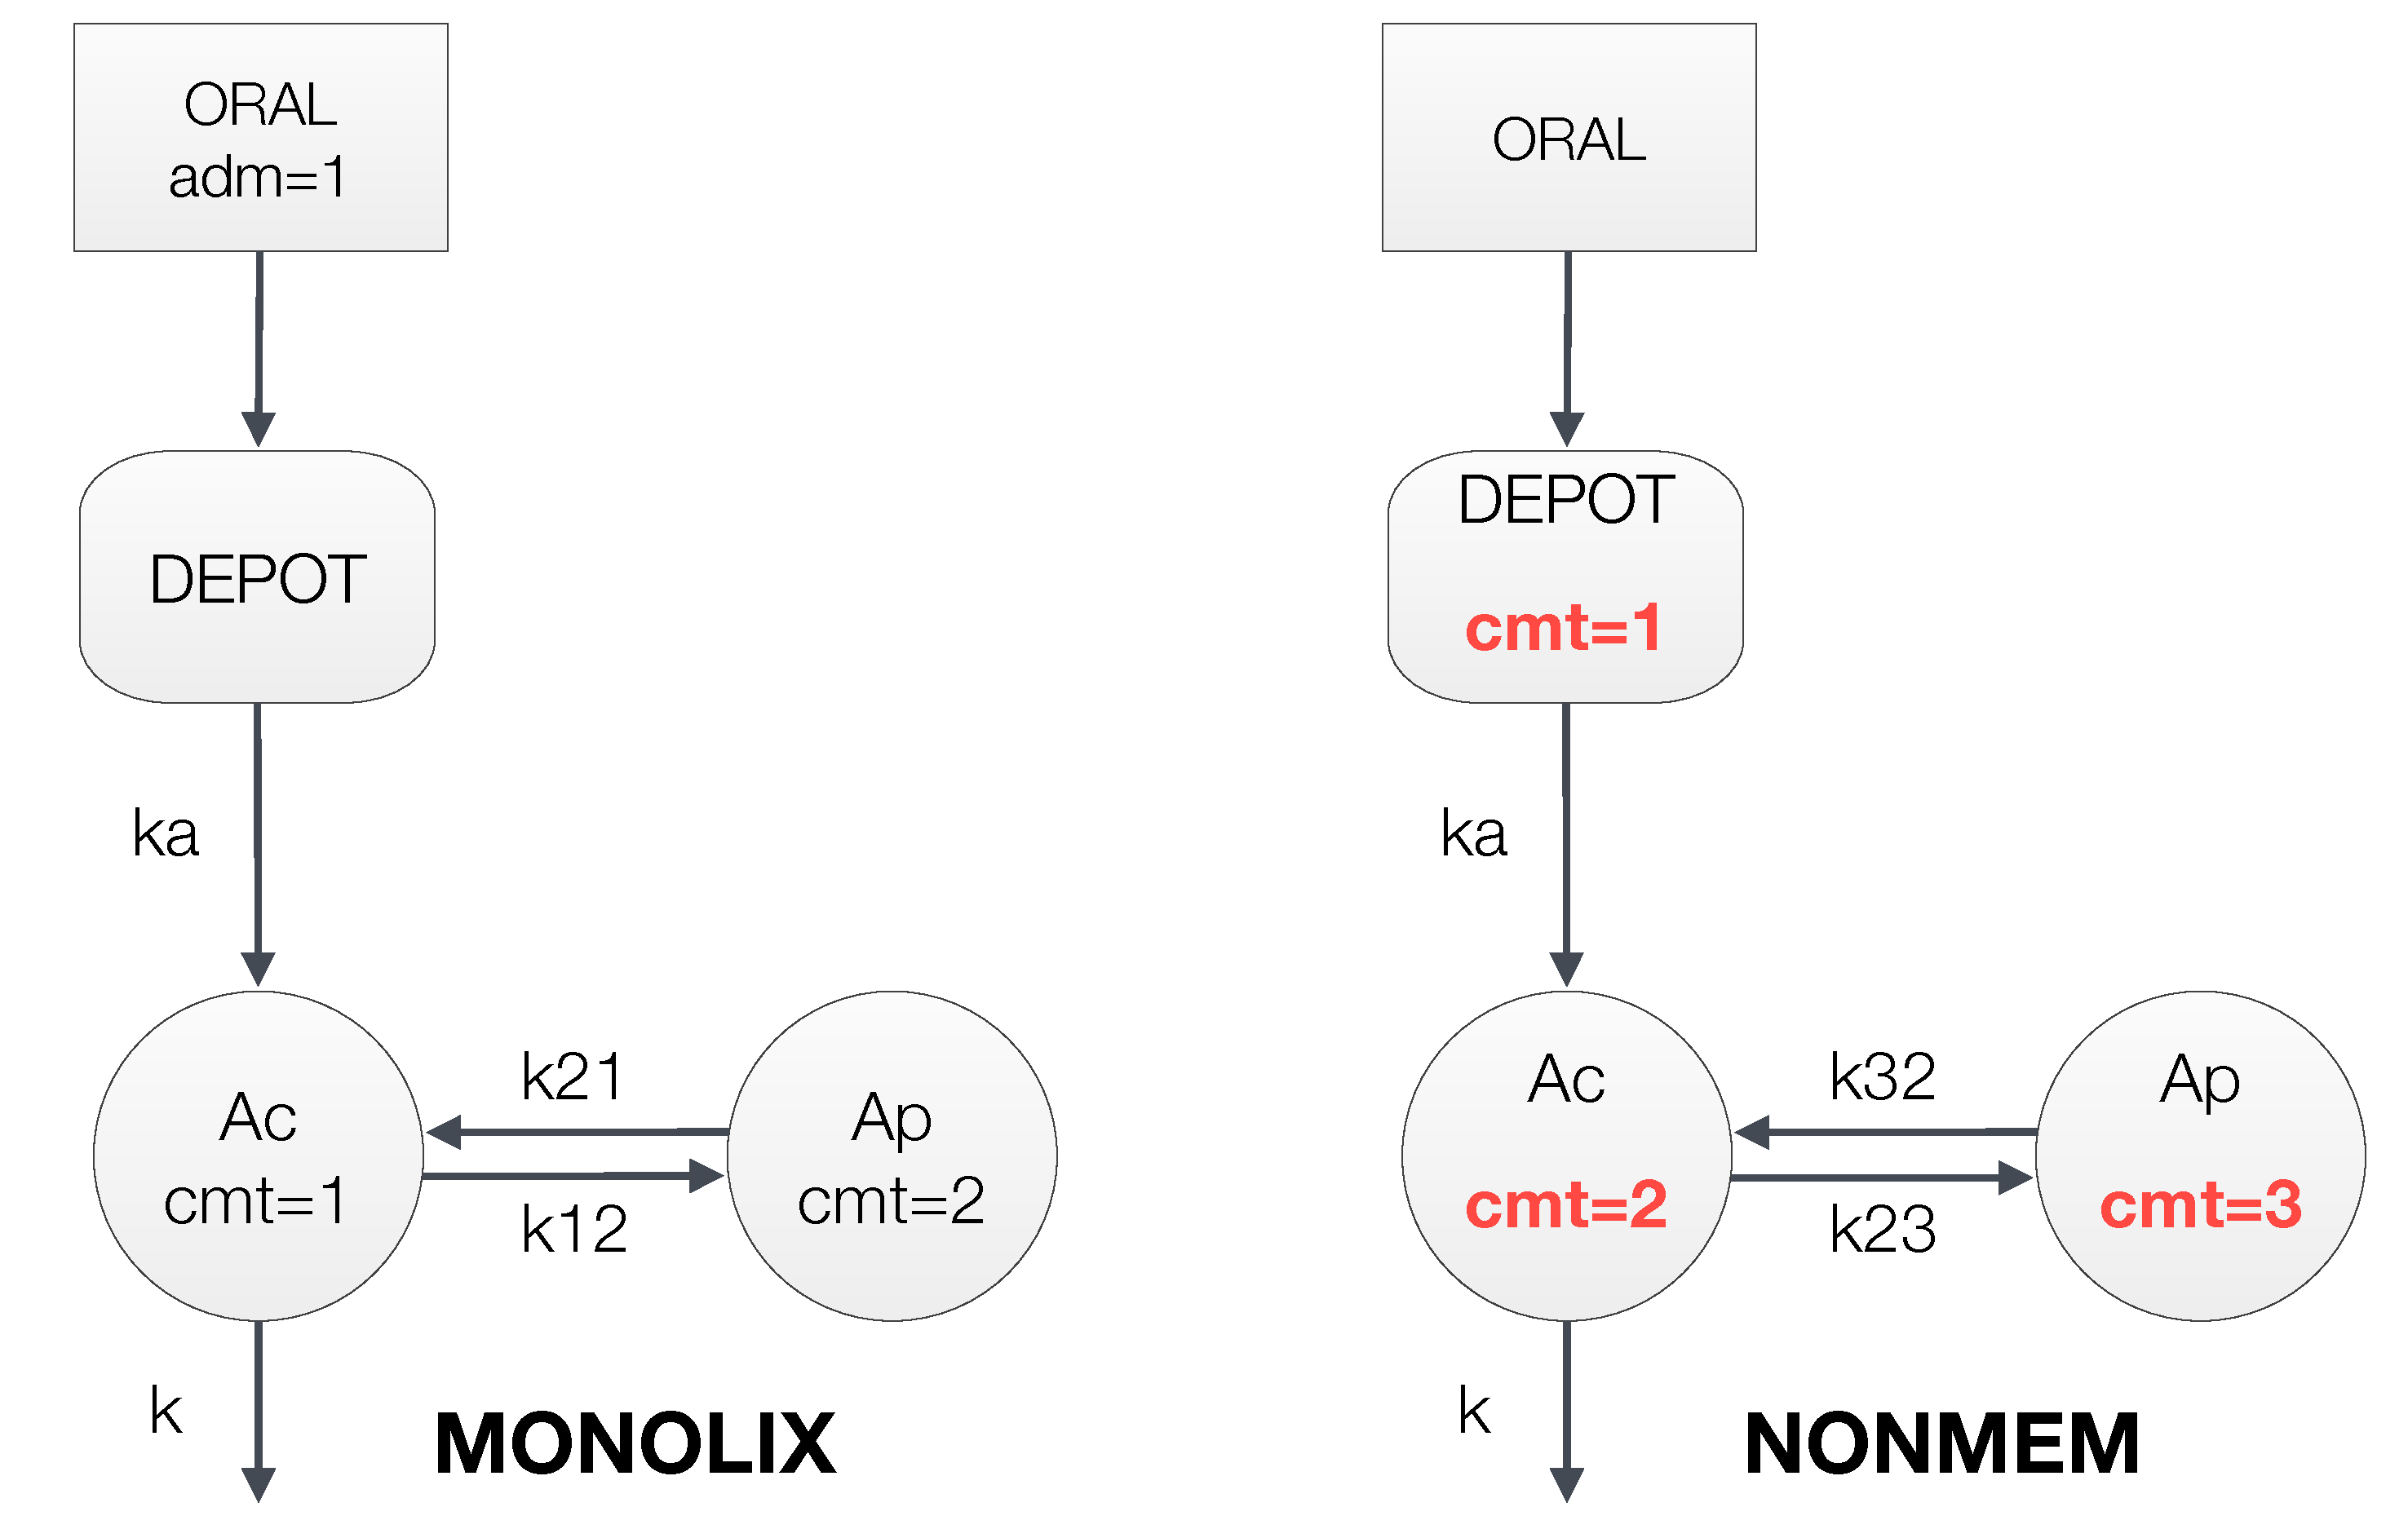
\includegraphics[width=110mm]{pics/Advan4.pdf}
\caption{ADVAN4 model, with compartment numbering dependent on the target tool. 
Note, that not only the compartment numbers are different in NONMEM coded model, 
the rate constants names are different as well.}
\label{fig:Advan4}
\end{figure}


\begin{table}[ht!]
\footnotesize
\parbox{.5\linewidth}{
\centering
\begin{tabular}{ccccc}
  \hline
   \multicolumn{5}{c}{\textbf{MONOLIX}} \\
  \hline
ID & TIME & AMT & \textbf{ADM} & Y \\
  \hline
1  & 0        & 10   & \textbf{1} & .       \\
1  & 2        & .      & . & 5        \\
... &  ...      &  ...   &  ...&  ...     \\
\end{tabular}
}
\hfill
\parbox{.5\linewidth}{
\centering
\begin{tabular}{ccccc}
  \hline
   \multicolumn{5}{c}{\textbf{NONMEM}} \\
  \hline
ID & TIME & AMT & \textbf{\textcolor{red}{CMT}} & DV \\
  \hline
1  & 0        & 10   & \textbf{\textcolor{red}{1}}   & .    \\
1  & 2        & .      & 2    & 5   \\
... &  ...      &  ...   &  ... & ...  \\
\end{tabular}
}
\caption{MONOLIX and NONMEM datasets for the ADVAN4 model.}
\end{table}

\begin{table}[h!]
\setlength{\tabcolsep}{15pt}
\begin{center}
%\begin{tabular*}{.95\textwidth}{@{\extracolsep{\fill} } ll}
\begin{tabular}{l}
  \hline \hline
PK macro  \\[-.25ex]
  \hline
\lstset{language=NONMEMdataSet}
\begin{lstlisting}
compartment(cmt=1, amount=Ac, volume=V)
peripheral(k12, k21, amount=Ap)
oral(adm=1, cmt=1, ka)
elimination(cmt=1, k)
\end{lstlisting}
%&
%\lstset{language=NONMEMdataSet}
%\begin{lstlisting}
%input = {ka, V, k, k12, k21}
%PK:
%compartment(cmt=1, amount=Ac, volume=V)
%[*compartment(cmt=3, amount=Depot)*]
%peripheral(k12, k21, amount=Ap)
%oral(adm=1, [*fromCmt=3,*] cmt=1, ka)
%elimination(cmt=1, k)
%\end{lstlisting} 
\\
  \hline
\end{tabular}
\caption{PK macros  for the ADVAN4 model, as shown in Figure \ref{fig:Advan4} (left).}
\label{tab:advan4Table}
\end{center}
\end{table}

PharmML code:
\lstset{language=XML}
\begin{lstlisting}
        <StructuralModel blkId="sm4">
            <ct:Variable symbolType="real" symbId="Ac"/>
            <ct:Variable symbolType="real" symbId="Ap"/>
            <ct:Variable symbolType="real" symbId="Cc">
                <ct:Assign>
                    <math:Equation>
                        <math:Binop op="divide">
                            <ct:SymbRef symbIdRef="Ac"/>
                            <ct:SymbRef blkIdRef="pm1" symbIdRef="V"/>
                        </math:Binop>
                    </math:Equation>
                </ct:Assign>
            </ct:Variable>
            <PKmacros>
                <Compartment>
                    <Value argument="cmt">
                        <ct:Int>1</ct:Int>
                    </Value>
                    <Value argument="amount">
                        <ct:SymbRef symbIdRef="Ac"/>
                    </Value>
                    <Value argument="volume">
                        <ct:SymbRef blkIdRef="pm1" symbIdRef="V"/>
                    </Value>
                </Compartment>
                <Peripheral>
                    <Value>
                        <ct:SymbRef blkIdRef="pm1" symbIdRef="k12"/>
                    </Value>
                    <Value>
                        <ct:SymbRef blkIdRef="pm1" symbIdRef="k21"/>
                    </Value>
                    <Value argument="amount">
                        <ct:SymbRef symbIdRef="Ap"/>
                    </Value>
                </Peripheral>
                <Oral>
                    <Value argument="adm">
                        <ct:Int>1</ct:Int>
                    </Value>
                    <Value argument="cmt">
                        <ct:Int>1</ct:Int>
                    </Value>
                    <Value>
                        <ct:SymbRef blkIdRef="pm1" symbIdRef="ka"/>
                    </Value>
                </Oral>
                <Elimination>
                    <Value argument="cmt">
                        <ct:Int>1</ct:Int>
                    </Value>
                    <Value>
                        <ct:SymbRef blkIdRef="pm1" symbIdRef="k"/>
                    </Value>
                </Elimination>
            </PKmacros>
        </StructuralModel>
\end{lstlisting}


%%%%%%%%%%%%%%%%%%%%%%%%%%%%%%%%%%%%%%%%%%%%%%%%%%%%%%%%%%%%%%%%%%%%%%
\subsection{ADVAN12, TRANS1 -- 3-comp 1st order input}
\label{subsubsec:ADVAN12}
ODE formulation:
\begin{align}
\frac{dAd}{dt} & =  -ka \times Ad \nonumber \\
\frac{dAc}{dt} & = ka \times Ad - k_{12} \times Ac + k_{21} \times Ap1 - k_{13} \times Ac \nonumber \\
			& + k_{31} \times Ap2 - k \times Ac  \nonumber \\
\frac{dAp1}{dt} & =  k_{12} \times Ac - k_{21} \times Ap1  \nonumber \\
\frac{dAp2}{dt} & =  k_{13} \times Ac - k_{31} \times Ap2  \nonumber
\end{align}

\begin{figure}[htbp!]
\centering
 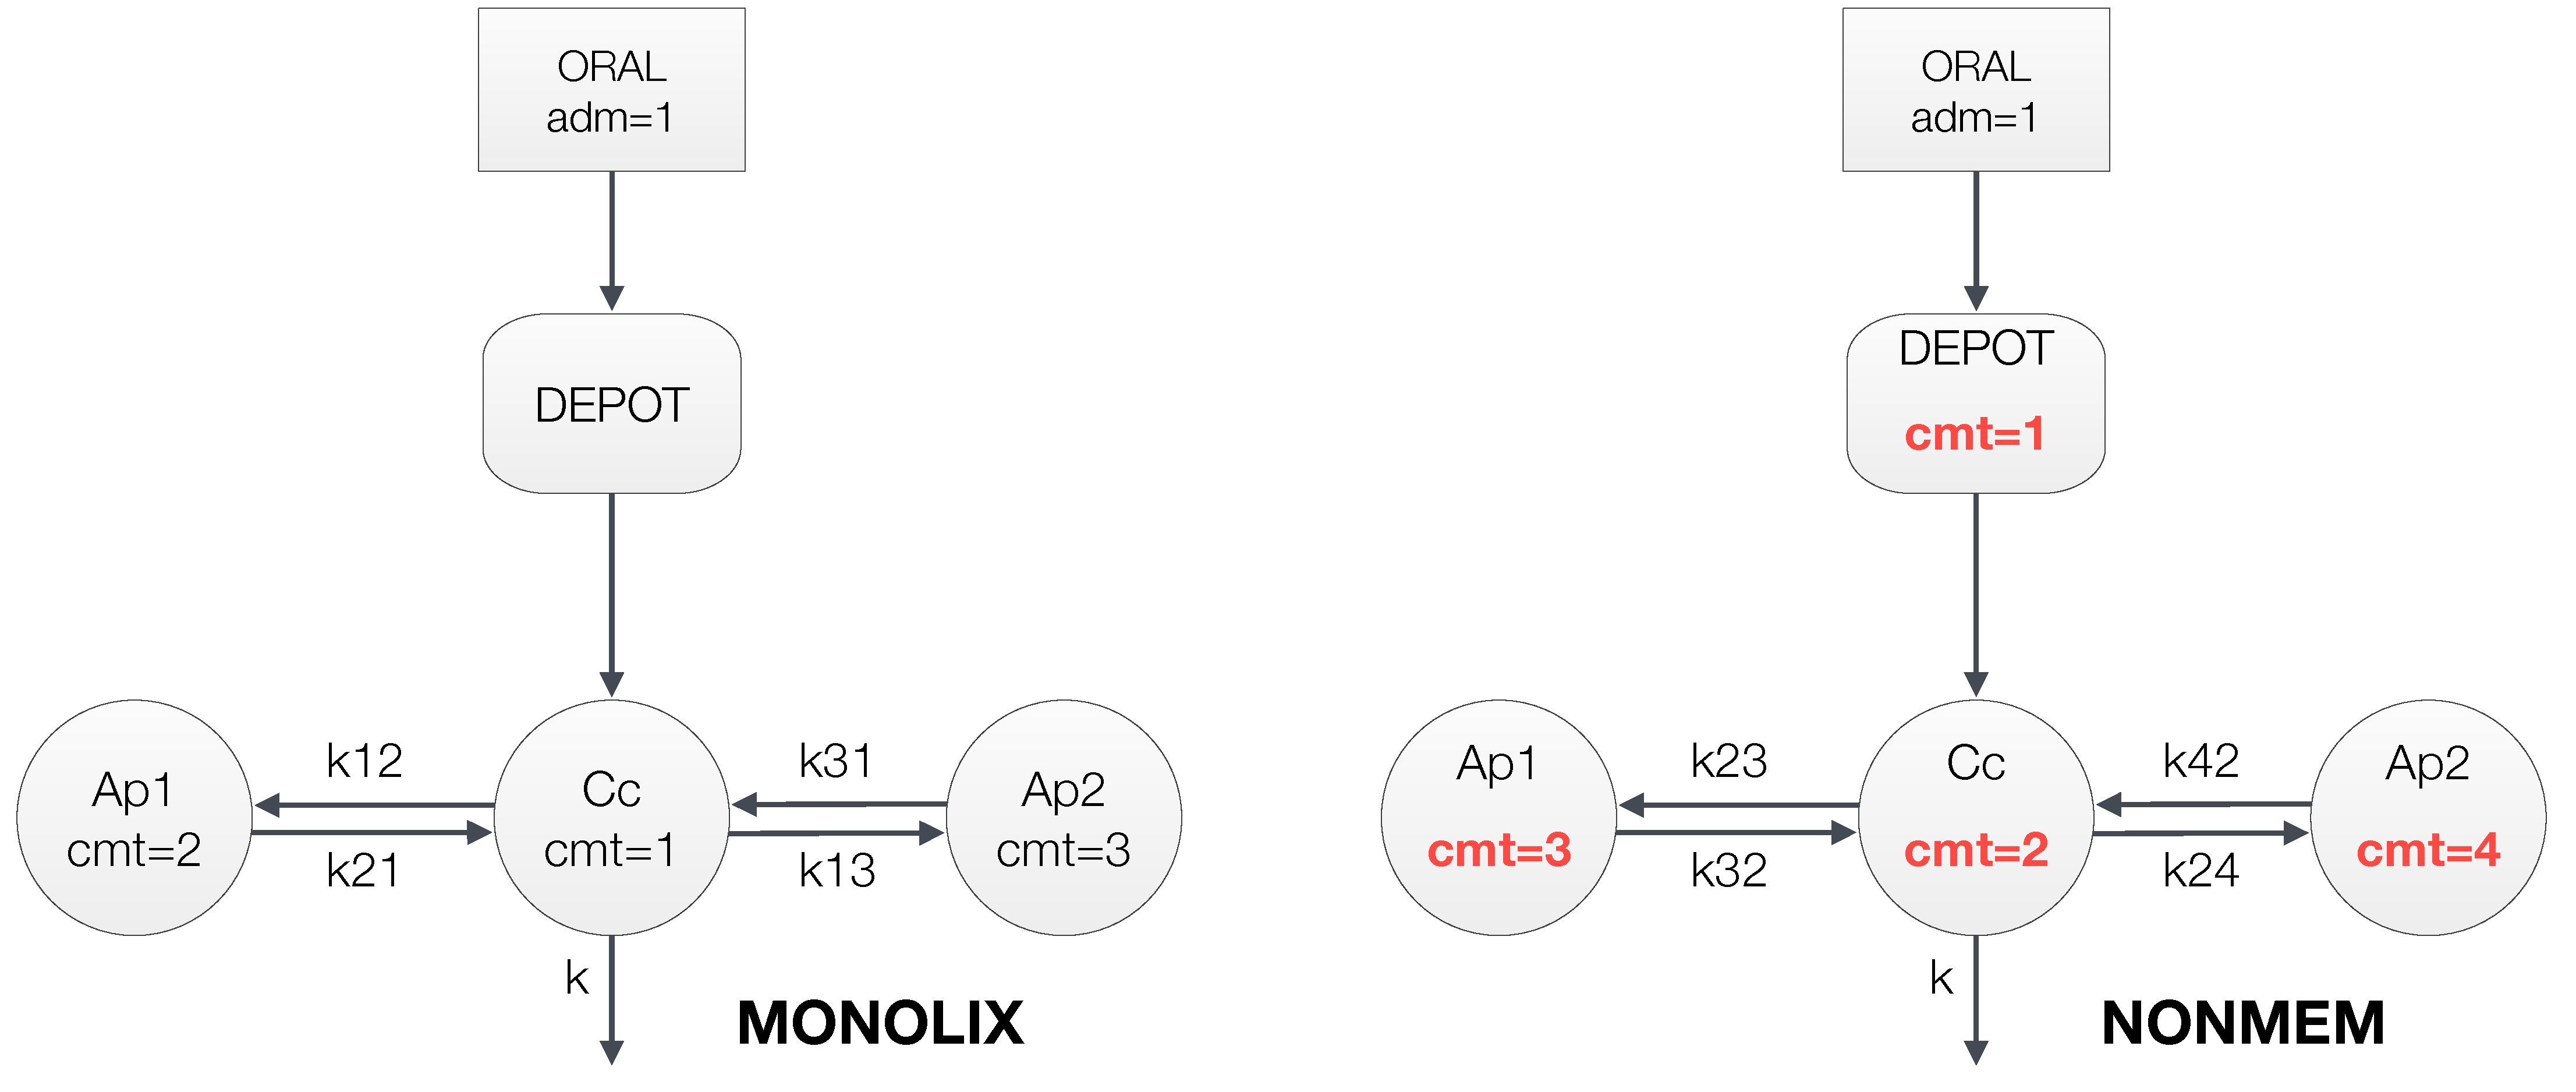
\includegraphics[width=160mm]{pics/Advan12.pdf}
\caption{ADVAN12 model, with compartment numbering dependent on the target tool. 
Note, that not only the compartment numbers are different in NONMEM coded model, 
the rate constants names are different as well.}
\label{fig:Advan12}
\end{figure}


\begin{table}[ht!]
\footnotesize
\parbox{.5\linewidth}{
\centering
\begin{tabular}{ccccc}
  \hline
   \multicolumn{5}{c}{\textbf{MONOLIX}} \\
  \hline
ID & TIME & AMT & \textbf{ADM} & Y \\
  \hline
1  & 0        & 10   & \textbf{1} & .       \\
1  & 2        & .      & . 	& 5        \\
... &  ...      &  ...   &  ...  &  ...     \\
\end{tabular}
}
\hfill
\parbox{.5\linewidth}{
\centering
\begin{tabular}{ccccc}
  \hline
   \multicolumn{5}{c}{\textbf{NONMEM}} \\
  \hline
ID & TIME & AMT & \textbf{\textcolor{red}{CMT}} & DV \\
  \hline
1  & 0        & 10   & \textbf{\textcolor{red}{1}}   & .    \\
1  & 2        & .      & 2    & 5   \\
... &  ...      &  ...   &  ... & ...  \\
\end{tabular}
}
\caption{MONOLIX and NONMEM datasets for the ADVAN12 model.}
\end{table}


\begin{table}[h!]
\setlength{\tabcolsep}{15pt}
\begin{center}
%\begin{tabular*}{.95\textwidth}{@{\extracolsep{\fill} } ll}
\begin{tabular}{l}
  \hline \hline
PK macro \\[-.25ex]
  \hline
\lstset{language=NONMEMdataSet}
\begin{lstlisting}
compartment(cmt=1, amount=Ac, volume=V)
peripheral(k12, k21, amount=Ap1)
peripheral(k13, k31, amount=Ap2)
oral(adm=1, cmt=1, ka)
elimination(cmt=1, k)
\end{lstlisting}
\\
  \hline
\end{tabular}
\caption{PK macros  for the ADVAN12 model, as shown in Figure \ref{fig:Advan12} (left).}
\label{tab:advan12Table}
\end{center}
\end{table}


PharmML code:
\lstset{language=XML}
\begin{lstlisting}
        <StructuralModel blkId="sm12">
            <ct:Variable symbolType="real" symbId="Ac"/>
            <ct:Variable symbolType="real" symbId="Ap1"/>
            <ct:Variable symbolType="real" symbId="Ap2"/>
            <ct:Variable symbolType="real" symbId="Cc">
                <ct:Assign>
                    <math:Equation>
                        <math:Binop op="divide">
                            <ct:SymbRef symbIdRef="Ac"/>
                            <ct:SymbRef blkIdRef="pm1" symbIdRef="V"/>
                        </math:Binop>
                    </math:Equation>
                </ct:Assign>
            </ct:Variable>
            
            <PKmacros>
                <Compartment>
                    <Value argument="cmt">
                        <ct:Int>1</ct:Int>
                    </Value>
                    <Value argument="amount">
                        <ct:SymbRef symbIdRef="Ac"/>
                    </Value>
                    <Value argument="volume">
                        <ct:SymbRef blkIdRef="pm1" symbIdRef="V"/>
                    </Value>
                </Compartment>
                <Peripheral>
                    <Value>
                        <ct:SymbRef blkIdRef="pm1" symbIdRef="k12"/>
                    </Value>
                    <Value>
                        <ct:SymbRef blkIdRef="pm1" symbIdRef="k21"/>
                    </Value>
                    <Value argument="amount">
                        <ct:SymbRef symbIdRef="Ap1"/>
                    </Value>
                </Peripheral>
                <Peripheral>
                    <Value>
                        <ct:SymbRef blkIdRef="pm1" symbIdRef="k13"/>
                    </Value>
                    <Value>
                        <ct:SymbRef blkIdRef="pm1" symbIdRef="k31"/>
                    </Value>
                    <Value argument="amount">
                        <ct:SymbRef symbIdRef="Ap2"/>
                    </Value>
                </Peripheral>
                <Oral>
                    <Value argument="adm">
                        <ct:Int>1</ct:Int>
                    </Value>
                    <Value argument="cmt">
                        <ct:Int>1</ct:Int>
                    </Value>
                    <Value>
                        <ct:SymbRef blkIdRef="pm1" symbIdRef="ka"/>
                    </Value>
                </Oral>
                <Elimination>
                    <Value argument="cmt">
                        <ct:Int>1</ct:Int>
                    </Value>
                    <Value>
                        <ct:SymbRef blkIdRef="pm1" symbIdRef="k"/>
                    </Value>
                </Elimination>
            </PKmacros>
        </StructuralModel>
\end{lstlisting}
\subparagraph{Note} A detailed description of all remaining predefined PREDPP models 
(ADVAN 1-3, 10, 11), alternative parameterizations other then the default TRANS1 as well 
aa more complex examples of macro implementation can be found in a technical report 
\cite{PKmacros:2015a} on PharmML related websites \url{http://ddmore.eu/pharmml} or 
\url{http://pharmml.org}.




\chapter{Language Overview}
\label{chap:lang-overview}

\section{Introduction}

This chapter provides the background knowledge 
to understand \pharmml. We recommend that you read this chapter
before working through the examples in chapter
\ref{chap:worked-egs}. The chapter starts by describing how a
\pharmml document is organised and then go on to illustrate some of
the key concepts and constructs of the language. For example, among
other things, we discuss variable and parameter scoping (section
\ref{sec:scoping-rules}), how to write maths (sections~\ref{sec:odes}
and~\ref{sec:maths}), and how to define data (section~\ref{subsec:inlineDataset}).
%and how to define and use units (section~\ref{sec:units}).
The chapter concludes with a discussion of the additional resources that
we expect to be used in support of \pharmml, but which are outside the
scope of this language specification (section~\ref{sec:supporting-res}).

\section{Organisation of \pharmml}
\label{sec:structure-overview}

\pharmml is organised into three main sections (\ref{fig:momloverview}): \emph{Model Definition}, \emph{Trial
  Design} and \emph{Modelling Steps}. This reflects the natural
organisation of a pharmacometric model and is the organisation
implicitly found in the M\&S tools used by modellers in this
area. Below we detail the purpose and
organisation of each section.

\begin{figure}[htb!]
 \centering
  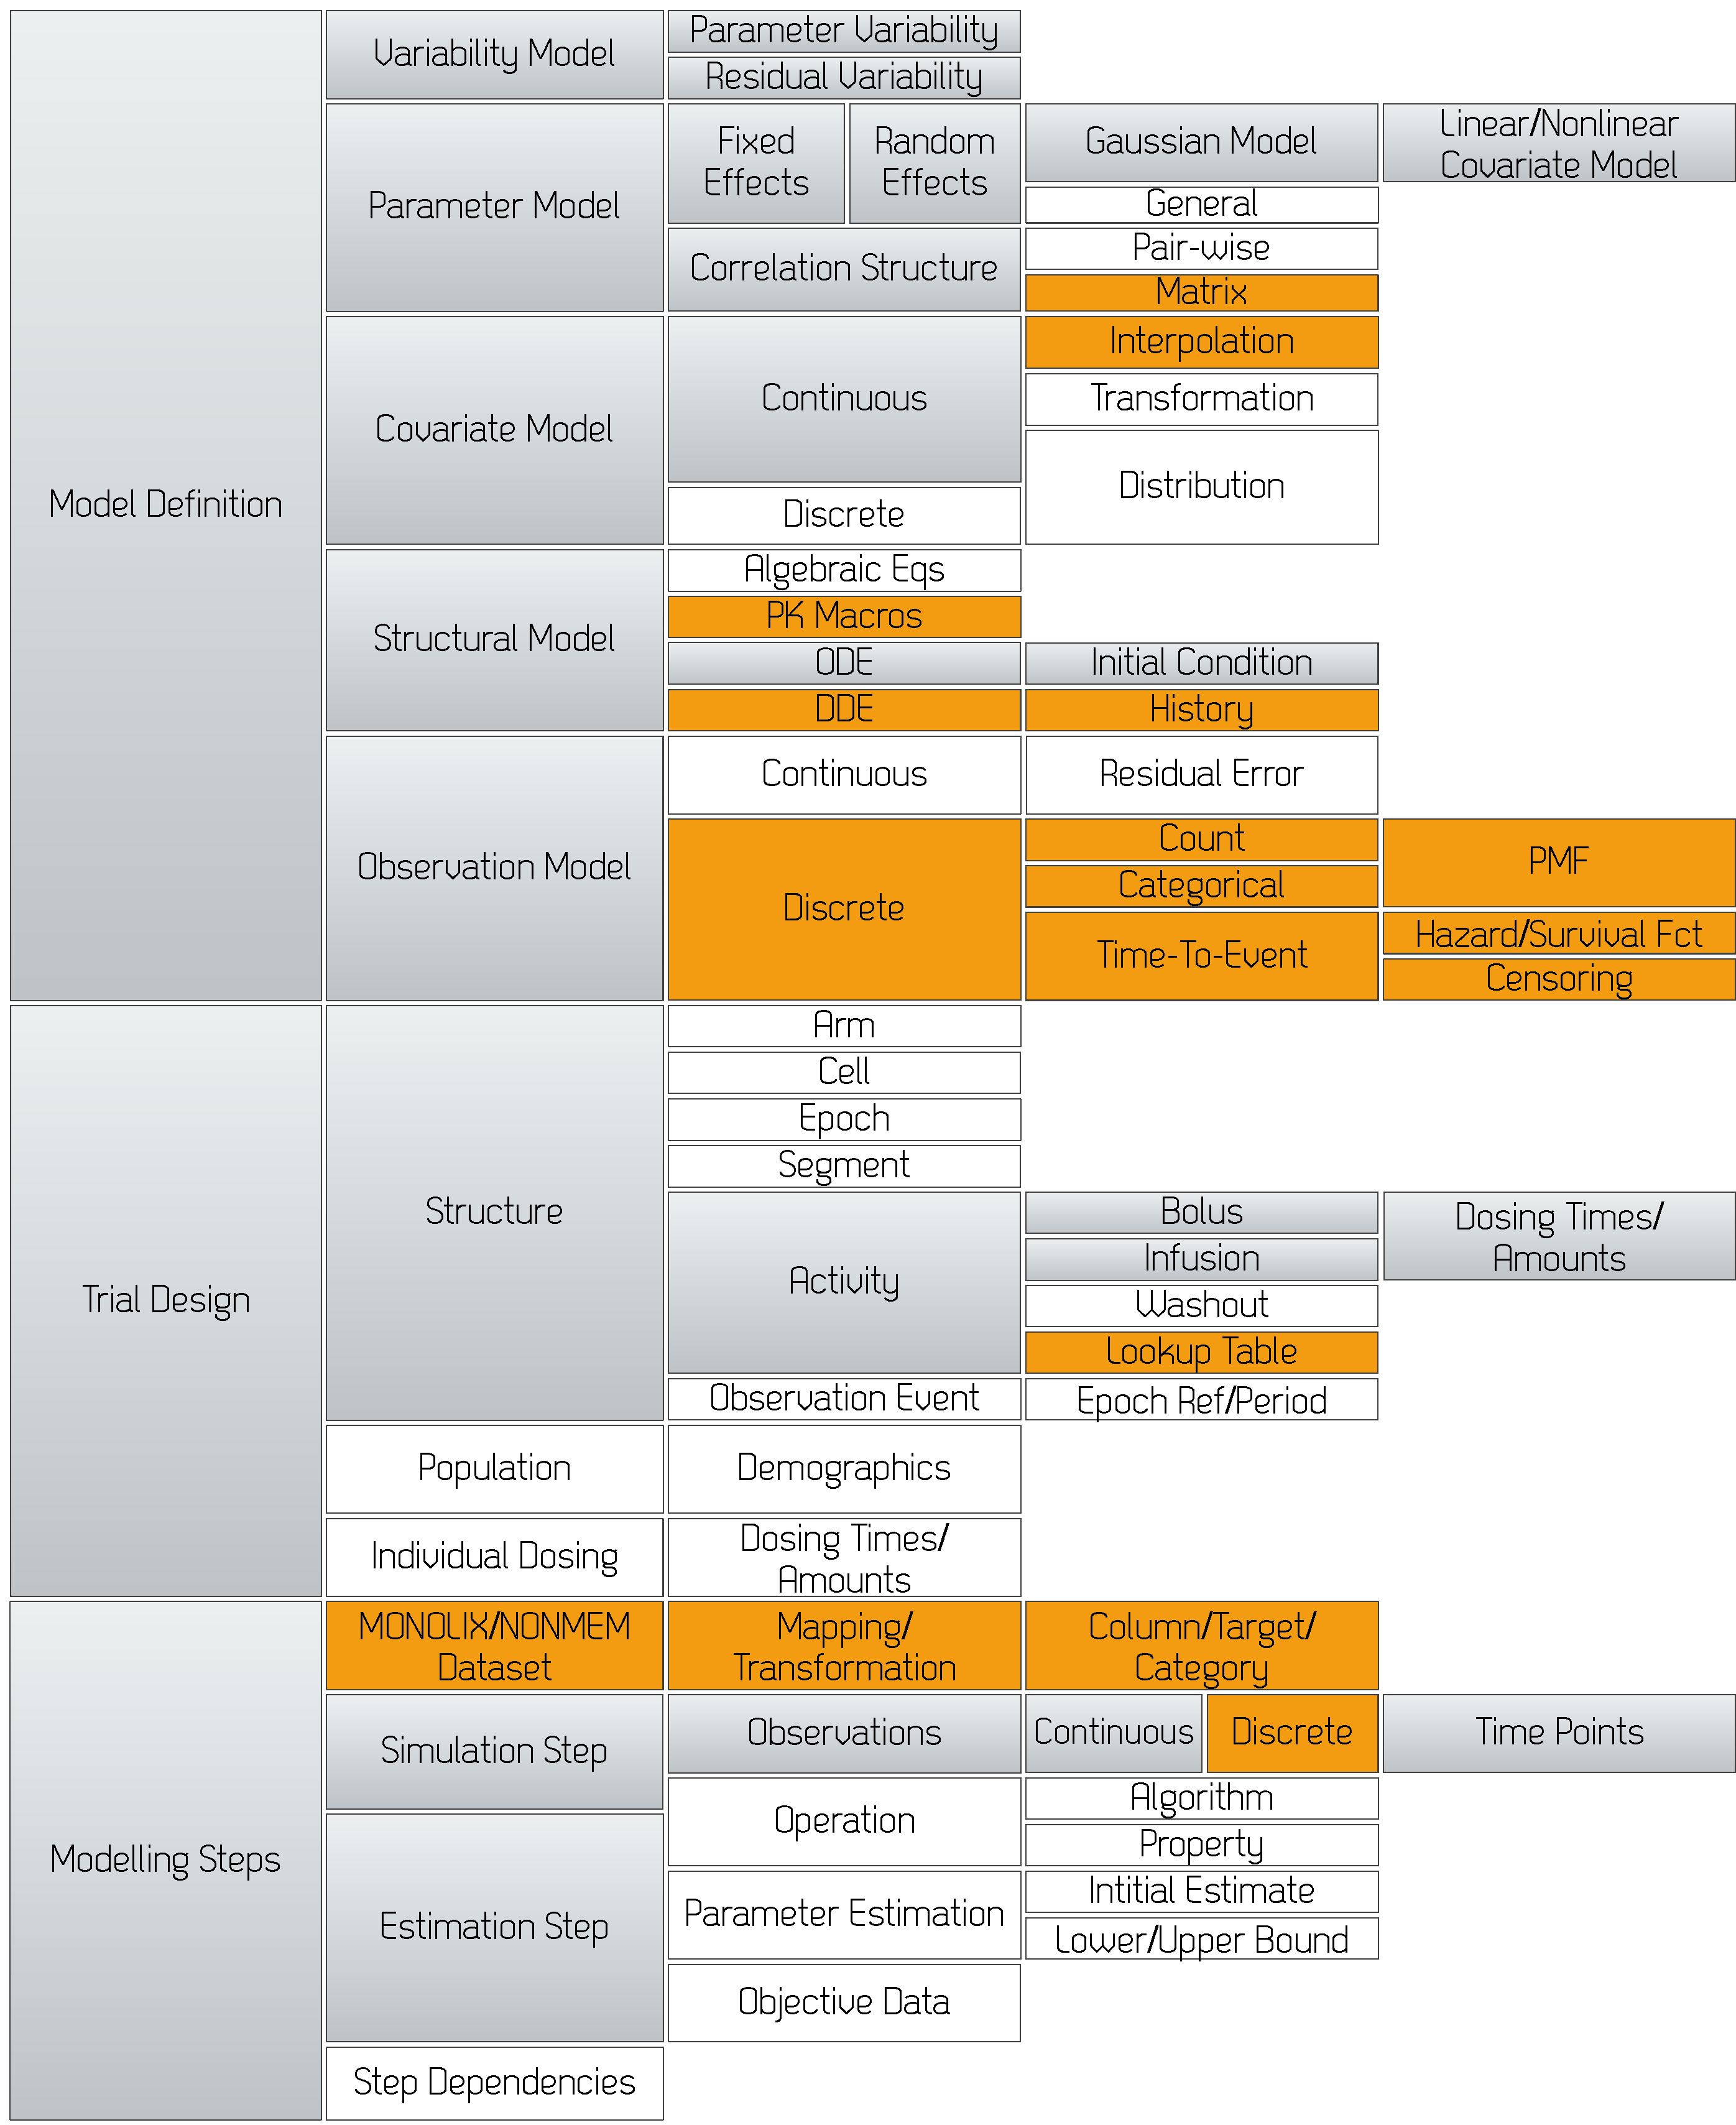
\includegraphics[height=0.85\textheight]{pics/PharmMLschemaOverview} % OverviewOfPharmML
  \caption{An overview of the organisation of \pharmml. The orange highlighted cells illustrate the 
  	new elements introduced in this specification compared to the first public version 0.2.1. 
	Grey indicate minor changes or extensions.}
  \label{fig:momloverview}
\end{figure}

\subsection{Model Definition}

The \emph{Model Definition} defines the model, typically a population
model, that describes the system under investigation and any variability
between individuals in the population. The modeller may wish to use
it for simulation, parameter estimation or other types of analysis and
exploration. The \emph{Model Definition} in turn is composed of another
set of ``models'' that describe specific aspects of the overall model
definition. These are described below.

\subsubsection{Variability Model}
\label{sec:variability_model}

Variability is the concept that underpins a pharmacometric model and
the \emph{Variability Model} enables us to describe this. Note that it
is possible to describe variability in a \pharmml model without
defining random variability, but by using covariates.
Therefore the use of the \emph{Variability Model}
is optional. In \pharmml you can use this to define
individual random variability, but also a hierarchy of variability
above and/or below the level of the individual (e.g.\xspace inter-occasion
variability). For more details of the theory behind the random
variability model, see section \ref{sec:variabilityModel}.


\subsubsection{Covariate Model}

The \emph{Covariate Model} describes the covariates, both continuous and discrete, 
to be used in the \emph{Parameter Model} (figure \ref{fig:momloverview}). 
This defines a transformation, interpolation or probability distribution 
for a covariate. The formal description of the covariate
model can be found in section \ref{maths:covariate_model}.

\subsubsection{Parameter Model}

The \emph{Parameter Model} principally describes the parameters of the model
definition and is typically used to describe parameters with some
level of variability (typically between subject variability). The
parameter is defined more formally in section
\ref{maths:parameter_defn}, but essentially for each parameter we
define a population term, one or more random effects, and its
relationship to the covariates defined in the covariate model. The
random effects can be defined at different levels of variability
(defined by the variability model, see section
\ref{sec:variability_model}), which includes capturing their correlation
structure by providing a covariance (or correlation)
matrix for each level of variability.

\subsubsection{Structural Model}

At the heart of the model definition are one or more \emph{Structural
Model}s. These describe the system or systems that a modeller is
interested in and they represent a particular abstraction of that
system. For example a structural model may be used to describe the
pharmacokinetics of a drug. We can represent PK, PD or PK-PD models as
combinations of ODEs and algebraic equations. For compartmental
PK models an alternative coding options are the PK macros, as described
in the chapter \ref{sec:PKMacros}.
\subsubsection{Observation Model}

In clinical trials experimental observations are made, and these
observations are subject to experimental error. Different types of
instrument, assay or material sampled will all have different
statistical errors associated with them. In a pharmacometric model
these errors are described using a residual error model (see
section~\ref{maths:error_model}). In \pharmml we encode the residual
error model using the \emph{Observation Model}.


The outcomes of a clinical trial that we wish to model are not always
experimental measurements. A trial may aim to determine the efficacy
of an analgesic using a pain score provided by the subject; or measure
the frequency of seizure based on the maximum drug concentration; or
establish the remission rate over a given time in a cancer trial
\cite{Bonate:2011fk}. In each of these cases one needs to use a
discrete statistical model to represent these outcomes. These are also
defined in the Observation Model.

\subsection{Trial Design}
\label{sec:trialdesign_model}

Clinical trials are carefully structured and can vary considerably in
their complexity. Typically, a trial will be structured into one or
more arms with each arm subject to one or more treatment regimens
and observation protocols. Each arm is then populated with individuals
from a population of subjects who have been screened for their
suitability to participate in the trial. In \pharmml we have two options: 1)
the NONMEM/Monolix dataset to inform the model about the 
design, dosing and observation records, 2) \xelem{TrialDesign} section is used 
to describe the trial structure and subject population explicitly.
The latter option is a novel approach making the clinical trial much clearer 
to document, easier to encode computationally and to use for simulations 
or optimal design. More information can be found in chapter~\ref{sec:CTS}.

\begin{figure}[htb!]
 \centering
  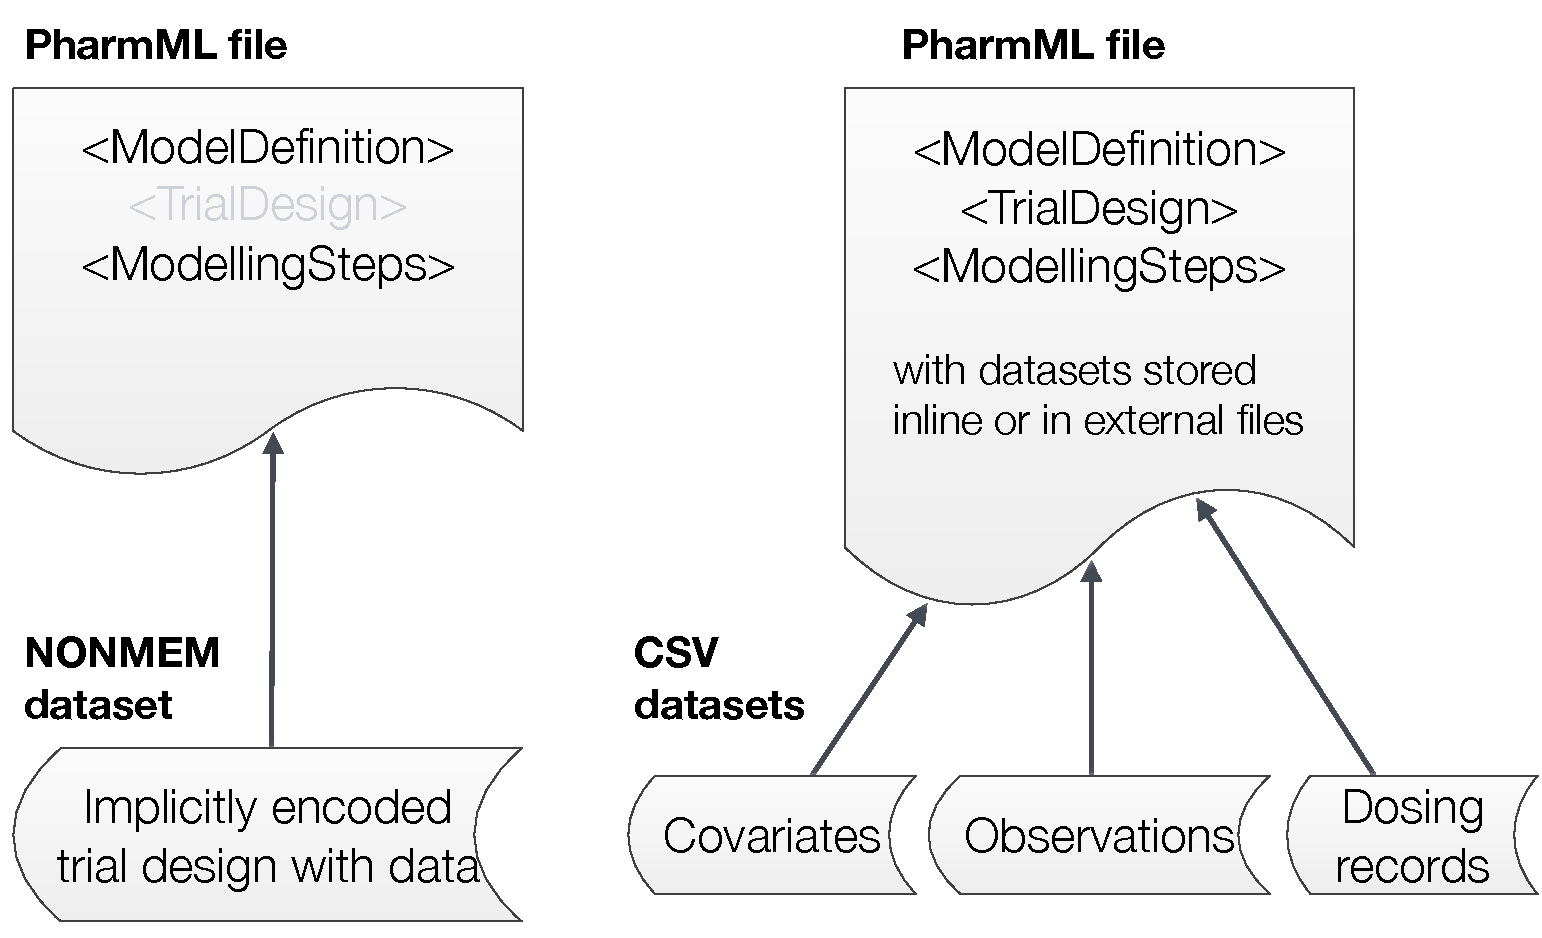
\includegraphics[width=0.5\textheight]{pics/DataVersusTrialDesign}
  \caption{Alternative ways to work with \pharmml -- either the information about the 
  underlying trial design and experimental records are sourced from a NONMEM type
  dataset or the trial design structure is encoded explicitly with datasets (covariates, 
  observation and dosing records) stored inline within the \pml model file or external 
  CSV files, see also Figure \ref{fig:dataStudyTaskFlow} for more details.}
  \label{fig:DataVersusTrialDesign}
\end{figure}

\begin{figure}[htb!]
 \centering
  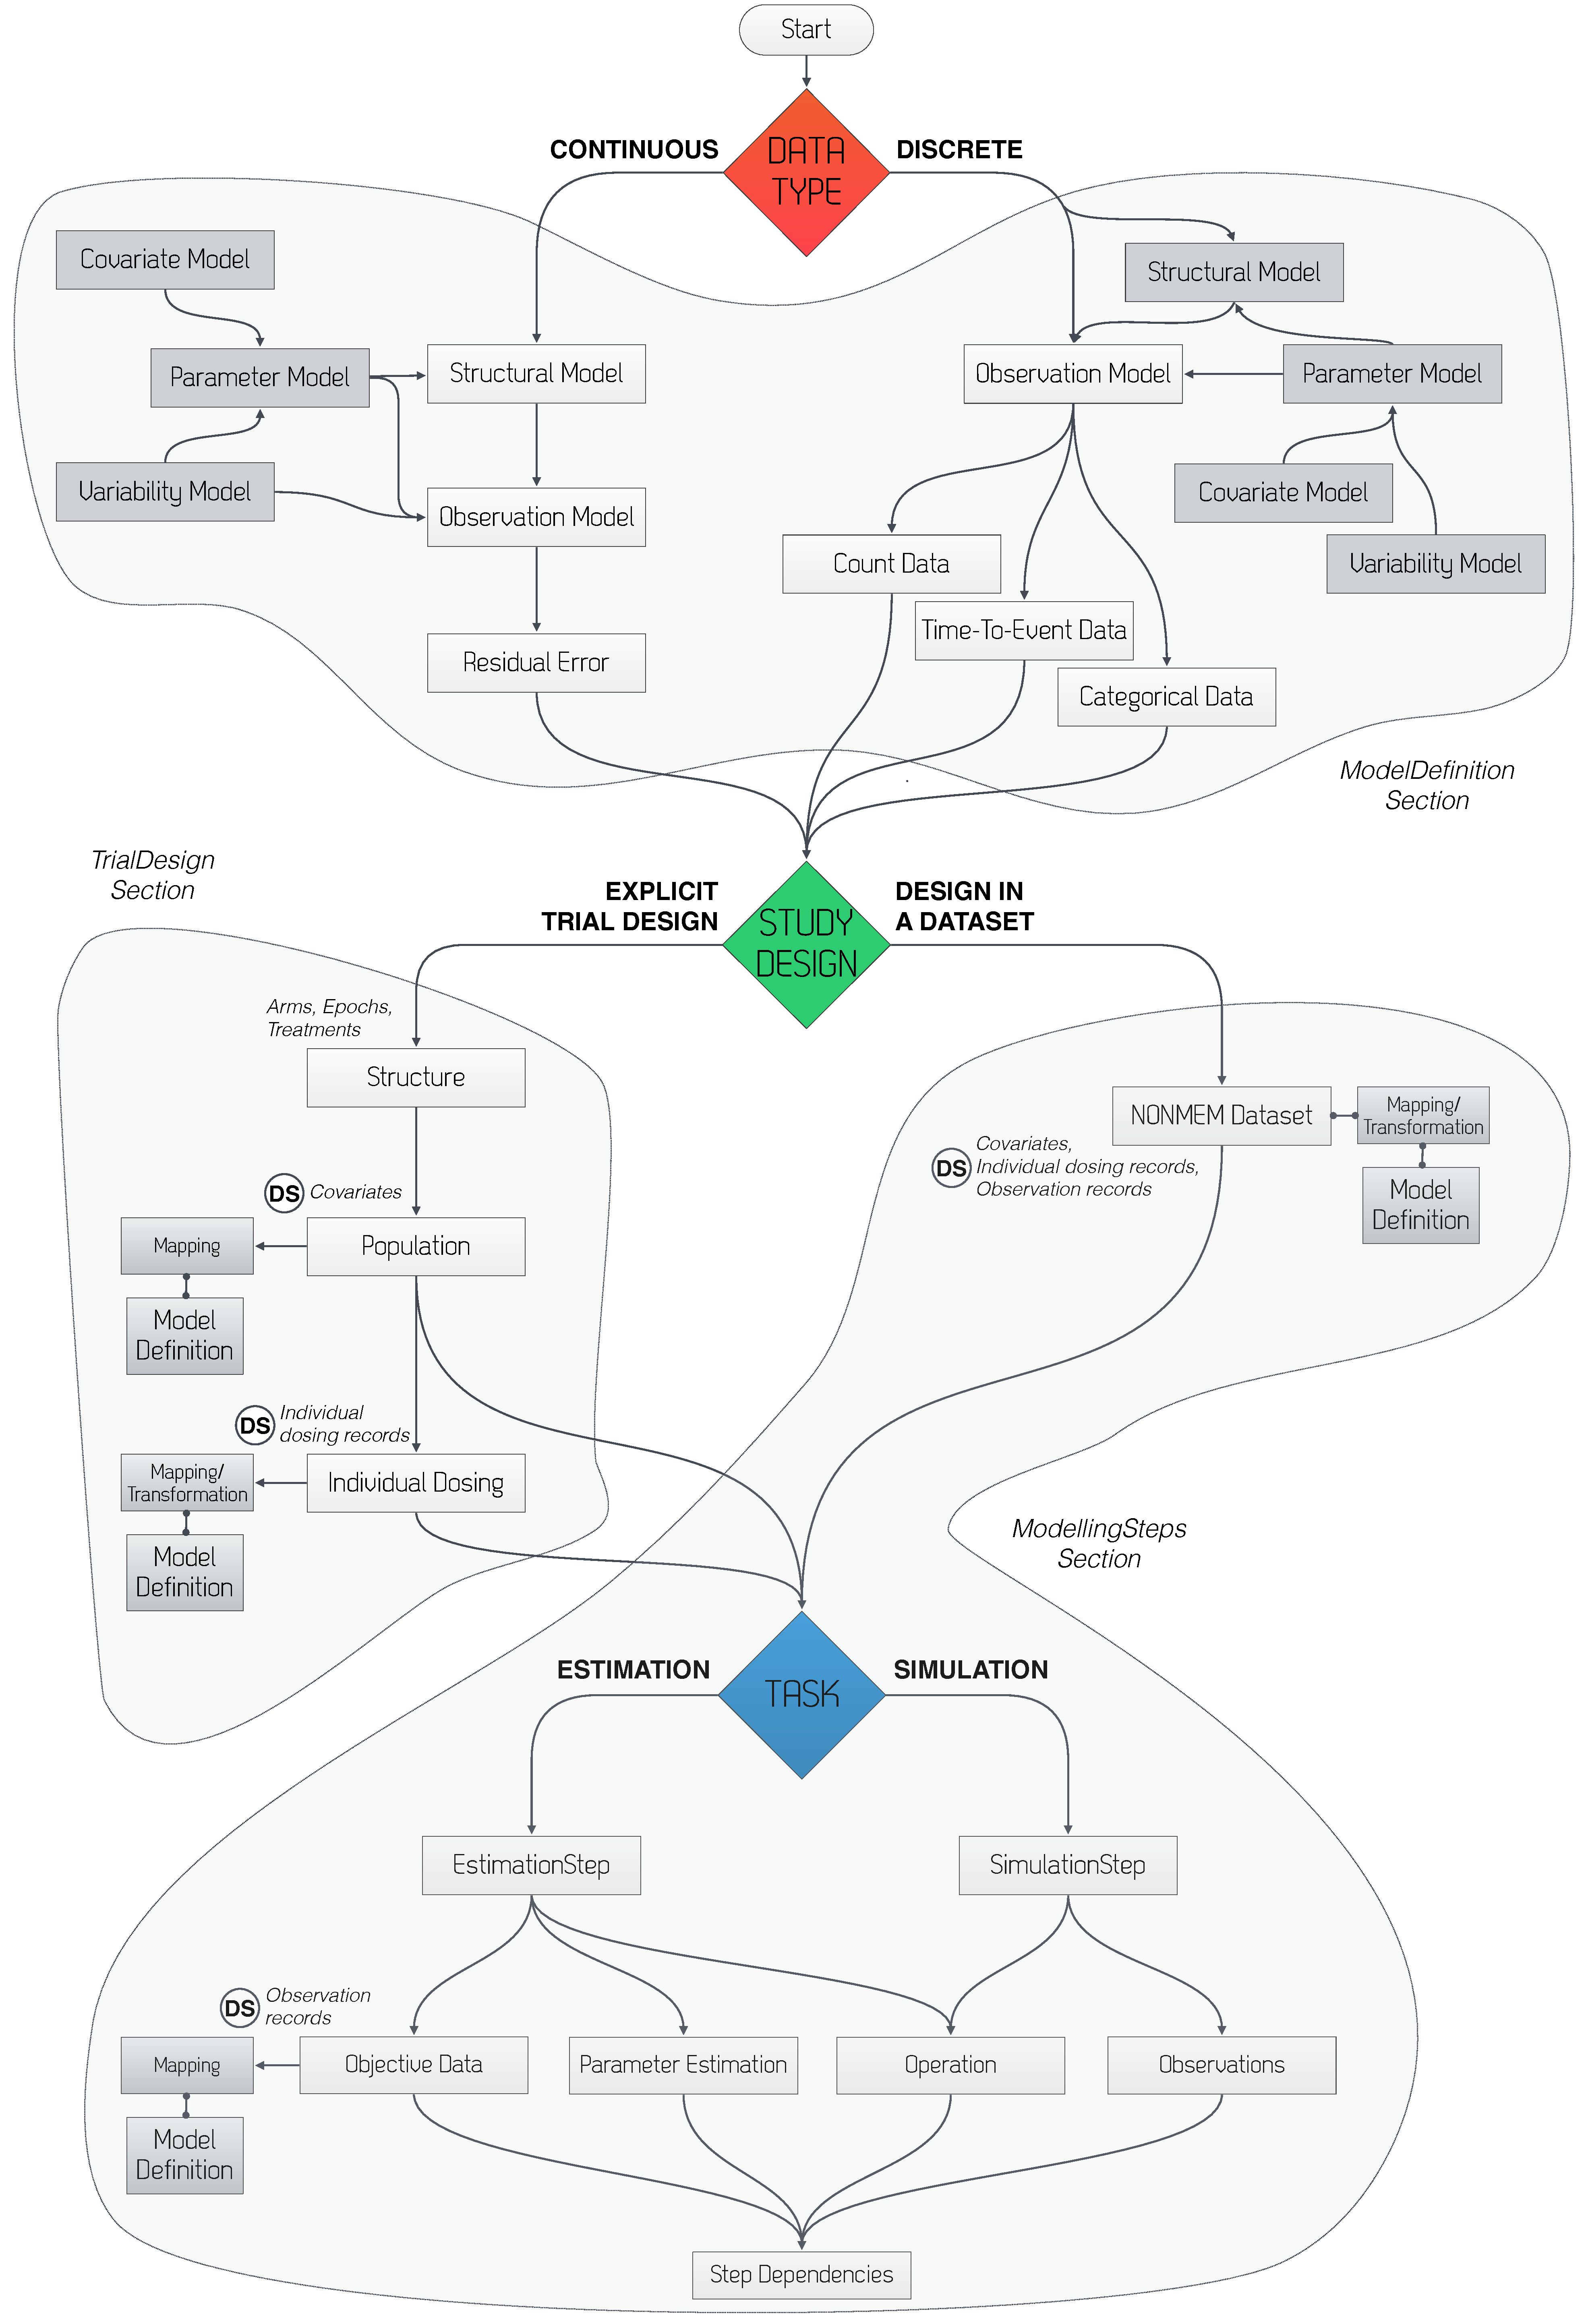
\includegraphics[height=0.90\textheight]{pics/Flowchart-dataTypeStudyTask}
  \caption{Working with \pharmml -- schema showing three essential decision points:
  the type of data (continuous and discrete), the source of the study design and data 
  (NONMEM dataset or \xelem{TrialDesign}) and finally the task type 
  (for now only simulation and estimation tasks are supported).}
  \label{fig:dataStudyTaskFlow}
\end{figure}

%%%%%%%%%%%%%%%%%%%%%%%%%%%%%%%%%%%%%%%%%%%%%%%%%%%%%%%%%%%%%%%%%%%%%%
\subsection{Modelling Steps}
\label{sec:stepdeps}
The final element when describing an M\&S experiment, after defining
the model and the associated trial design, is to describe how the
model was used. This section of a \pharmml document is akin to the
Methods section of a paper. The aim is not to replicate your modelling
exactly, but to provide enough information to reproduce the
model\footnote{To replicate the execution of a model requires detailed
  information about not only what algorithms were used to simulate or
  execute a model, but also what software implementation was used and
  exact supporting libraries such as that of the random number
  generator.}.

%%%%%%%%%%%%%%%%%%%%%%%%%%%%%%%%%%%%%%%%%%%%%%%%%%%%%%%%%%%%%%%%%%%%%%
\section{Identifiers, references and namespaces}

In \pharmml we use the Object Identifier \xatt{oid} to identify components in the
\emph{Trial Design} and \emph{Modelling Steps} sections of a \pharmml document and
the Symbol Identifier \xatt{symbId} to identify parameters and variables within the
\emph{Model Definition} section. Below we will describe the rules associated
with how they are defined and referenced.


%%%%%%%%%%%%%%%%%%%%%%%%%%%%%%%%%%%%%%%%%%%%%%%%%%%%%%%%%%%%%%%%%%%%%%
\subsection{Object identifiers}

The concept of the Object Identifier is borrowed from the CDISC XML
description of a trial design \cite{CDISC:2011a}. There they use the
attribute \xatt{oid} to identify and to reference components used in
the design. Object identifiers have global scope, which means that all
object identifiers defined in a \pharmml document must be unique.

Elements that reference an object identifier by convention use the
attribute \texttt{oidRef} and the id referred to must exist in the
\pharmml document. In addition the object referred to must be
compatible with the element referencing it. The example below shows
how this works:
%
\lstset{language=XML}
\begin{lstlisting}
<Epoch oid="e1">
  <!-- Detail omitted -->
</Epoch>
<Arm oid="a2">
  <!-- Detail omitted -->
</Arm>
<Cell oid="c2">
    <EpochRef oidRef="e1" />
    <ArmRef oidRef="a2"/>
    <SegmentRef oidRef="tb"/>
</Cell>
\end{lstlisting}
%
Here the element \xelem{EpochRef} refers to the object identifier of
the Epoch, ``e1'', and the \xelem{ArmRef} element refers to the Arm
object, ``a2''. This is correct. However, the following example
is incorrect:
%
\lstset{language=XML}
\begin{lstlisting}
<Epoch oid="e1">
  <!-- Detail omitted -->
</Epoch>
<Arm oid="a2">
  <!-- Detail omitted -->
</Arm>
<Cell oid="c2">
    <!-- ERROR: not valid PharmML -->
    <EpochRef oidRef="a2" />
    <ArmRef oidRef="a2"/>
    <SegmentRef oidRef="tb"/>
</Cell>
\end{lstlisting}
%
The \xelem{EpochRef} points to the Arm object, which is not compatible
with it. Note that this cannot be validated using SML Schema. 
These compatibilities are documented for each element
containing an object reference (i.e.\xspace an \xatt{oidRef}
attribute) in the XML Schema. 


%%%%%%%%%%%%%%%%%%%%%%%%%%%%%%%%%%%%%%%%%%%%%%%%%%%%%%%%%%%%%%%%%%%%%%
\subsection{Blocks and symbol scoping}
\label{sec:blocks}
\label{sec:scoping-rules}

\pharmml defines names for the
parameters, variables and parts of the model that need to be uniquely
identified. In \pharmml we refer to these collectively as symbols. The
rules we apply are relatively simple in that all symbols within a
\pharmml document must be unique and that all symbols in the document are
`visible'. In other words a symbol defined in one part of a document
will be available to a component elsewhere in the document. Symbols in
\pharmml can be organised into different scopes, which in turn are
defined by blocks. We illustrate this conceptually in the example
below\footnote{Note that in the example we use the element
  \xelem{Symbol} to define a symbol and \xelem{Block} a block. These
  are not actually valid \pharmml elements, but we hope to make the
  scoping discussion clearer by using these.}:

\lstset{language=XML}
\begin{lstlisting}
<Block blkId="blockID">
	...
	<Symbol symbId="symbolID">
		...
	</Symbol>
	...
        <SymbRef symbIdRef="symbolID"/>
</Block>

<ElsewhereInXMLDocument>
	<SymbRef blkIdRef="blockID" symbIdRef="symbolID"/>
</ElsewhereInXMLDocument>
\end{lstlisting}
The block is given an identifier and is used to organise symbols. Any
symbols that are defined within it are part of the block's scope (private symbols). If
we refer to that symbol within the block then we do not need to specify the
block name. When referred to outside the block, then the same symbol
must be referred to using a combination of the block identifier
(\xatt{blkId}) and symbol identifier (\xatt{symbId}). This is illustrated
more completely in the example below:

\lstset{language=XML}
\begin{lstlisting}
<Symbol symbId="symb2"/> <!-- Decl 1 -->
<Symbol symbId="symb3"/> <!-- Decl 2 -->

<Block blkId="A">
	<Symbol symbId="symb2"/> <!-- Decl 3 -->
        <SymbRef symbIdRef="symb2"/> <!-- resolves to Decl 3 -->
        <SymbRef symbIdRef="symb3"/>  <!-- resolves to Decl 2 -->
</Block>

<Block blkId="B">
	<Symbol symbId="symb2"/>  <!-- Decl 4 -->
	<Symbol symbId="symb3"/> <!-- Decl 5 -->
        <SymbRef symbIdRef="symb2"/>  <!-- resolves to Decl 4 -->
</Block>

<ElsewhereInXMLDocument>
	<SymbRef symbIdRef="symb2"/> <!-- resolves to Decl 1 -->
	<SymbRef blkIdRef="A" symbIdRef="symb2"/> <!-- resolves to Decl 3 -->
	<SymbRef blkIdRef="B" symbIdRef="symb2"/> <!-- resolves to Decl 4 -->
	<SymbRef blkIdRef="B" symbIdRef="symb3"/> <!-- resolves to Decl 5 -->
</ElsewhereInXMLDocument>
\end{lstlisting}

Here, the \xelem{Symbol} element defines a symbol and \xelem{SymbRef}
refers to it.  As you can see, a symbol can be defined in several
places: globally (outside a block) and within blocks A and B. In each
case identical \xatt{symbID}s are used, but the language can
distinguish between them because of the context. This is clear when we
look at the symbol references in the \xelem{ElsewhereInXMLDocument}
element. Referring to a symbol, for example symbol \attval{symb2} in
block A may seem ambiguous, but the scoping rules of \pharmml are
clear. The reference is resolved first to the scope within the block
and then to the global scope. So in block A the reference to
\attval{symb2} points to Decl 3, and the reference to \attval{symb3}
points to the global symbol, Decl 2 and not Decl 5, which is a
different scope. These scoping rules are common to many programming
languages. One question you may ask is what if a globally defined symbol
has the same name as a block identifier? This is handled by the
symbol namespace rules. Both types of identifier share the same (global)
namespace and so cannot have the same name.

You will notice in the discussion above that we use the words `define'
and `reference'. These are important concepts in \pharmml. Symbols can be
\emph{defined} only once, but can be \emph{referred} to many
times. Symbols can be referred to before they are defined. 
\pharmml is a declarative language (unlike C or Fortran), thus it is natural
that the order of variable definition is not important. The listing below
shows how this works using real \pharmml.

\lstset{language=XML}
\begin{lstlisting}
<ct:Variable symbId="c" symbolType="real">
    <ct:Assign>
        <Equation xmlns="http://www.pharmml.org/pharmml/0.6/Maths">
            <Binop op="divide">
                <ct:SymbRef symbIdRef="b"/>
                <ct:Real>10</ct:Real>
            </Binop>
        </Equation>
    </ct:Assign>
</ct:Variable>
<ct:Variable symbId="a" symbolType="real">
    <ct:Assign>
        <Equation xmlns="http://www.pharmml.org/pharmml/0.6/Maths">
            <Binop op="plus">
                <ct:SymbRef symbIdRef="b"/>
                <ct:SymbRef symbIdRef="c"/>
            </Binop>
        </Equation>
    </ct:Assign>
</ct:Variable>
<ct:Variable symbId="b" symbolType="real">
    <ct:Assign>
        <ct:Real>1</ct:Real>
    </ct:Assign>
</ct:Variable>
\end{lstlisting}

One danger with this approach is that the language syntax does not
prevent the creation of cyclic dependencies between variables. An
example of this is shown below where there is dead-lock because neither variable can be initialised
because the other is yet to be defined. Such cycles are forbidden in
\pharmml and must be checked for when validating the language.
(See section \ref{subsec:AssinmentRules} with the description of related
validation rules, which are already or are supposed to be implemented 
and handled by 
libPharmML\footnote{\url{https://sourceforge.net/projects/libpharmml.ddmore.p}}, 
an API under development as part of the DDMoRe project.)
\lstset{language=XML}
\begin{lstlisting}
<!-- ERROR: The declaration below creates a cycle -->
<ct:Variable symbId="d" symbolType="real">
    <ct:Assign>
        <ct:SymbRef symbIdRef="e"/>
    </ct:Assign>
</ct:Variable>
<ct:Variable symbId="e" symbolType="real">
    <ct:Assign>
        <ct:SymbRef symbIdRef="d"/>
    </ct:Assign>
</ct:Variable>
\end{lstlisting}

Related to variable definition is the initialisation of a symbol: also
known as initial assignment. When a symbol is defined it is in an
uninitialised state and has no value. It may be either initialised
during the definition, as in the examples above, or via a subsequent
initial assignment as below:

\lstset{language=XML}
\begin{lstlisting}
<!-- Symbol defined, but not initialised -->
<ct:Variable symbId="a" symbolType="real"/>
<!--  Omitted detail -->
<ct:VariableAssignment>
    <ct:SymbRef  symbIdRef="a"/>
    <ct:Assign>
        <math:Equation>
            <math:Binop op="plus">
                <ct:SymbRef symbIdRef="a"/>
                <ct:Real>10</ct:Real>
            </math:Binop>
        </math:Equation>
    </ct:Assign>
</ct:VariableAssignment>
\end{lstlisting}

Either way this can only be done once. This listing illustrates the problem:
\lstset{language=XML}
\begin{lstlisting}
<!-- Symbol defined, but not initialised -->
<ct:Variable symbId="a" symbolType="real"/>
<!-- Snip -->

<!-- Incorrect -->
<!-- Duplicate initial assignments here. -->
<ct:VariableAssignment>
    <ct:SymbRef  symbIdRef="a"/>
    <ct:Assign>
        <ct:Real>0</ct:Real>
    </ct:Assign>
</ct:VariableAssignment>
<ct:VariableAssignment>
    <ct:SymbRef  symbIdRef="a"/>
    <ct:Assign>
        <math:Equation>
            <math:Binop op="plus">
                <ct:SymbRef symbIdRef="a"/>
                <ct:Real>10</ct:Real>
            </math:Binop>
        </math:Equation>
    </ct:Assign>
</ct:VariableAssignment>
\end{lstlisting}
\pharmml is a declarative language and the order is not important, 
thus symbols in \pharmml can only be initialised
once.


Note that in \pharmml symbol references between sections only go in one
direction. All sections point to the \emph{Model Definition}, but not
the reverse and the \emph{Modelling Steps} section points to the
\emph{Trial Design} section, but again not \emph{vice
  versa}\xspace. By maintaining this layered dependency structure in
the design of \pharmml we simplify the design of the language and ensure
that the \emph{Model Definition} section is guaranteed to be
independent of the other \pharmml sections.

\subsection{Interaction between Object and Symbol identifiers}

The Object and Block identifier (\xatt{oid} and \xatt{blkId}
respectively) both exist in the same \pharmml document and they share
the same namespace. This means that they cannot share the same
identifier, as is illustrated below:
%
\lstset{language=XML}
\begin{lstlisting}
<Symbol symbId="symb2"/>

<Block blkId="A"> <!-- ERROR -->
	<Symbol symbId="symb3"/>
</Block>

<Block blkId="B"> <!-- OK -->
	<Symbol symbId="symb4"/>
</Block>

<Oid oid="A"/> <!-- ERROR -->
<Oid oid="Z"/> <!-- OK -->
<Oid oid="symb2"/> <!-- ERROR -->
<Oid oid="symb3"/> <!-- OK -->
\end{lstlisting}
%
Similarly, just as a global \xatt{symbId} cannot share an identifier with a
\xatt{blkId} (see section~\ref{sec:scoping-rules}), neither can it
share an identifier (in the above case ``symb2'') with an \xatt{oid}.


%%%%%%%%%%%%%%%%%%%%%%%%%%%%%%%%%%%%%%%%%%%%%%%%%%%%%%%%%%%%%%%%%%%%%%
\section{Type checking}
\label{sec:type-checking}

Symbols in \pharmml have a type. By symbol we mean something defined
using a \xatt{symbId} attribute (for example a variable or
parameter). Like a variable a type is simply a way we use in \pharmml to
map symbols to an abstraction: such as a number, a string or a table
of values. As you might expect, symbols with different types are not
always compatible with each other, so it is necessary when validating
the correctness of a \pharmml document to ensure that the types of its
symbols are compatible with each other. This is known as type checking
(see \cite[Chapter6]{Aho:1986fk} and \cite[Chapter 8]{Parr:2010uq} for
more information). The types in \pharmml are enumerated in table
\ref{tab:type-specification}.


The types used in \pharmml must be consistent. In general this means that
all types in an expression should be identical. This is illustrated in
the following example:
%
\lstset{language=XML}
\begin{lstlisting}
<!-- ERROR: incompatible type -->
<ct:Variable symbId="a" symbolType="int">
    <ct:Assign>
        <ct:String>A value</ct:String>
    </ct:Assign>
</ct:Variable>
<ct:Variable symbId="b" symbolType="boolean"/>
<ct:Variable symbId="c" symbolType="real">
    <ct:Assign>
        <m:Equation>
            <m:Binop op="plus"> <!-- ERROR: Cannot add a real to a Boolean -->
                <ct:Real>22</ct:Real>
                <ct:SymbRef symbIdRef="b"/>
            </m:Binop>
        </m:Equation>
    </ct:Assign>
</ct:Variable>
<ct:Variable symbId="d" symbolType="real">
    <ct:Assign>
        <ct:Int>453</ct:Int> <!-- OK -->
    </ct:Assign>
</ct:Variable>
\end{lstlisting}
%
Note that the variable $d$ is of type real but was
initialised with an integer value, and that this was permitted. This
is an exception to the rule that all types must be the same and is
a common mechanism in computer languages, called type promotion. Here
the integer value can be converted to a real with no loss of
information and so it is permitted. The reverse conversion is not
permitted because a real value may lose information when converted to
an integer.


%%%%%%%%%%%%%%%%%%%%%%%%%%%%%%%%%%%%%%%%%%%%%%%%%%%%%%%%%%%%%%%%%%%%%
\section{Two ways to connect trial design and model}
\label{subsec:twoModes}
There are two basic options\footnote{In version 0.2.1 only the \xelem{TrailDesign}
based option was supported. This however proved to be very limiting for 
various reasons and support for NONMEM/Monolix datasets has been required.}  
to provide trial design related information in \pml. In the first the entire information 
is implemented in the \pml file, while in the second datasets with experimental 
data are used, see Figure \ref{fig:DataVersusTrialDesign} and \ref{fig:dataStudyTaskFlow}.

\begin{table}[h!]
\setlength{\tabcolsep}{15pt}
\begin{center}
\begin{tabular}{ll}
  \hline
 \xelem{TrialDesign} and inline datasets & External NONMEM dataset \\
  \hline
  \lstset{language=XML}
\begin{lstlisting}
<ModelDefinition>
    ...
</ModelDefinition>
<TrialDesing>
    <Structure>
        ...
    </Structure>
    <Population>
        ...
    </Population>
</TrialDesing>
<ModellingsSteps>
    <EstimationStep oid="est1">
        <ObjectiveDataSet>
            ...
        </ObjectiveDataSet>                
        ...
    </EstimationStep>
    ...
</ModellingsSteps>
\end{lstlisting}
&
\lstset{language=XML}
\begin{lstlisting}
<ModelDefinition>
    ...
</ModelDefinition>

<!-- TrailDesign section is not required -->

<ModellingsSteps>
    <ExternalDataSet toolName="NONMEM" oid="DSoid">
        ...
    </ExternalDataSet>
    
    <EstimationStep oid="est1">
        <ExternalDataSetReference>
            <ct:OidRef oidRef="DSoid"/>
        </ExternalDataSetReference>
        ...
    </EstimationStep>
    ...
</ModellingsSteps>
\end{lstlisting}  
\\
    \hline
\end{tabular}
\caption{Comparison of model structures encoded using \xelem{TrialDesign} 
(left) and using NONMEM format dataset (right). In the latter case the 
\xelem{TrialDesign} part is redundant and the complete information about 
the study design is sourced from the dataset. This holds for both estimation and 
simulation tasks.}
\label{tab:withAndWithoutNM}
\end{center}
\end{table}

Table \ref{tab:withAndWithoutNM} shows the \pml code for these two options 
as described in the following
\begin{itemize} 
\item
Using \xelem{TrialDesign}/\xelem{ModellingSteps} -- trial design (information about 
design arms, dosing times, amounts etc.) is encoded explicitly in XML and according 
experimental data records are provided within three datasets.
More specifically covariates and individual dosing records are encoded in 
the \xelem{Population} element of the \xelem{TrialDesign} section, while the
observation records, in \pml referred to as \xelem{ObjectiveDataSet}, are stored 
in \xelem{ModellingSteps}, see Table \ref{tab:withAndWithoutNM} (left).
\item
Using NONMEM/Monolix datasets -- these files contain the complete information 
about the underlying trial design, both for estimation or simulation tasks. 
Using datasets has consequences for the content of the \pml document 
in that the \xelem{TrialDesign} part is in such case redundant. Instead the dataset
is referenced in the \xelem{ExternalDataSet} element and referenced later in e.g.
estimation task, \xelem{ExternalDataSetReference}, see Table \ref{tab:withAndWithoutNM}
(right).
\end{itemize}


%%%%%%%%%%%%%%%%%%%%%%%%%%%%%%%%%%%%%%%%%%%%%%%%%%%%%%%%%%%%%%%%%%%%%%
\section{Datasets}
\label{sec:datasets}

The dataset is a key concept in PharmML and is used to describe the data 
of the relevant trial design, i.e. the observations, covariates and dosing
records. 
The data is tabular and the dataset has therefore been designed to 
represent this type of information and all data is explicitly typed.


%%%%%%%%%%%%%%%%%%%%%%%%%%%%%%%%%%%%%%%%%%%%%%%%%%%%%%%%%%%%%%%%%%%%%%
\subsection{Inline datasets}
\label{subsec:inlineDataset}
We start with the data implemented entirely within the \pml file. As usual 
the simplest way to explain it is to look at an example, such as the code 
snippet below:
\lstset{language=XML}
\begin{lstlisting}
<ds:DataSet>
    <ds:Definition>
        <ds:Column columnId="id" columnType="id" valueType="string" columnNum="1"/>
        <ds:Column columnId="arm" columnType="arm" valueType="string" columnNum="2"/>
        <ds:Column columnId="reps" columnType="replicate" valueType="int" columnNum="3"/>
    </ds:Definition>
    <ds:Table>
        <ds:Row>
            <ct:String>i1</ct:String><ct:String>a1</ct:String><ct:Int>20</ct:Int>
        </ds:Row>
        <ds:Row>
            <ct:String>i2</ct:String><ct:String>a2</ct:String><ct:Int>20</ct:Int>
        </ds:Row>
        <ds:Row>
            <ct:String>i3</ct:String><ct:String>a3</ct:String><ct:Int>40</ct:Int>
        </ds:Row>
        <ds:Row>
            <ct:String>i4</ct:String><ct:String>a4</ct:String><ct:Int>40</ct:Int>
        </ds:Row>
    </ds:Table>
</ds:DataSet>
\end{lstlisting}
%
The dataset starts with \xelem{Definition} where the columns of the
dataset table are defined. For each column the following attributes have to be 
specified
\begin{itemize} 
\item
\xatt{columnId} -- the name of the column  
\item
\xatt{columnType} --  the type of the column identifies 
the role the stored item plays in the model, see Table \ref{tab:MDLPharmML_columnTypes}
for the explanation of allowed values.  

\item
\xatt{valueType} -- the type of each column value is specified, which
complies with the \pharmml type system.  
\item
\xatt{columnNum} -- the column number must start at 1 and each
column must be numbered in consecutive order (i.e.\xspace 1,2,3,4\ldots etc.). 
\end{itemize}
Next the content of the dataset is held within the \xelem{Table} element and 
this consists of one or more \xelem{Row} elements. Each row must contain 
an entry for each column defined. This approach is based on the concept of 
a relation in relational theory. Therefore the ordering of rows is not significant. 

\begin{table}[ht!]
\begin{center}
\begin{tabular}{ll}
  \hline
\xatt{columnType} & Meaning \\  
  \hline
addl  & number of additional doses     \\
adm  & type of administration     \\
arm &     study arm \\
censoring  & left-censored data     \\
covariate  & covariates     \\
cmt & target compartment \\
demographic &     demographic type \\
dose  & dose      \\
duration & infusion duration \\
dv  & dependent variable     \\
dvid  & mixed observations     \\
epoch &     study epoch \\
evid  &  dose events     \\
id   & subject identifiers      \\
idv   & independent variable     \\
ii   & inter-dose interval     \\
limit  & lower limit for interval-censored data     \\
mdv  & missing dependent variable     \\
occasion   & occasions     \\
rate   & infusion rate     \\
reg   & regression variable     \\
replicate &     in cases when subjects are assumed identical \\
ss   & steady state \\
ssEndTime &     steady-state administration end time \\
ssPeriod &     steady-state administration interval \\
time  & time     \\
undefined & value for any undefined cases \\
   \hline
\end{tabular}
\caption{A summary of allowed values for the \xatt{columnType} attribute in \pml.}
\label{tab:MDLPharmML_columnTypes}
\end{center}
\end{table}


%%%%%%%%%%%%%%%%%%%%%%%%%%%%%%%%%%%%%%%%%%%%%%%%%%%%%%%%%%%%%%%%%%%%%%
\subsection{NONMEM/Monolix datasets}
\label{subsec:externalDataset}
Inline storage of data split into three tables has disadvantages in that 
it requires provision of additional translation tools to convert standard 
datasets to this format. Editing such data sets by hand is 
very error prone and time consuming.

There was a lot of request for supporting external datasets, more specifically
those used by NONMEM, Monolix and other tools. 
As shown in the following listing, the external data set can be specified using the 
new \xelem{ImportData} element, instead of \xelem{Table}, by providing the file 
path relative to the \pml file. Optional parameters such as file format and 
delimiter can also be provided. The external file must be a valid input file for the target tool.
%\emph{CSV}, with four delimiters: \xatt{COMMA}, \xatt{SEMICOLON}, \xatt{SPACE} 
%and \xatt{TAB}. 
The template for this reads: 
\lstset{language=XML}
\begin{lstlisting}
    <ds:ExternalFile oid="id1">
        <ds:path>FILE_PATH</ds:path>
        <ds:format>FORMAT</ds:format>
        <ds:delimiter>DELIMITER_TYPE</ds:delimiter>
    </ds:ExternalFile>
    \end{lstlisting}
And listing below shows a simple example how this works. As before the \xelem{Definition}
defines the table content and a reference to the according file and its type is provided.
\lstset{language=XML}
\begin{lstlisting}
    <ds:DataSet>
        <ds:Definition>
            <ds:Column columnId="ID" columnType="id" valueType="id" columnNum="1"/>
            <ds:Column columnId="ARM" columnType="arm" valueType="id" columnNum="2"/>
            <ds:Column columnId="SEX" columnType="covariate" valueType="id" columnNum="3"/>
            <ds:Column columnId="EPOCH" columnType="epoch" valueType="id" columnNum="4"/>
        </ds:Definition>
    	<ds:ExternalFile oid="id1">
	    <ds:path>warfarin_conc_pca.csv</ds:path>
            <ds:format>CSV</ds:format>
            <ds:delimiter>COMMA</ds:delimiter>
        </ds:ExternalFile>
    </ds:DataSet>
\end{lstlisting}

%%%%%%%%%%%%%%%%%%%%%%%%%%%%%%%%%%%%%%%%%%%%%%%%%%%%%%%%%%%%%%%%%%%%%%
\subsection{\xelem{TrialDesign} external datasets}
\label{subsec:TrialDesignExternal}

In the \xelem{TrialDesign} section the user has the choice between inline or
external dataset storage, see Section \ref{sec:trialdesign_model}.
External datasets can be specified using the \xelem{ImportData} element. 
As shown in the example below, you must provide the file path relative to the PharmML file, 
file format (only CSV files allowed) and one of the allowed delimiters (\xatt{COMMA}, 
\xatt{SEMICOLON}, \xatt{SPACE}, \xatt{TAB}). Further validation rules are listed in xxx.

\lstset{language=XML}
\begin{lstlisting}
            <ds:ExternalFile oid="id1">
                <ds:path>/datasets/myData.csv</ds:path>
                <ds:format>CSV</ds:format>
                <ds:delimiter>COMMA</ds:delimiter>
            </ds:ExternalFile>
\end{lstlisting}



%%%%%%%%%%%%%%%%%%%%%%%%%%%%%%%%%%%%%%%%%%%%%%%%%%%%%%%%%%%%%%%%%%%%%%
\subsection{Lookup table}
\label{subsec:lookupTable}

\xelem{TrialDesign} can be used to define a wide range of dosing scenarios 
which can be used to encode virtually any PK model. Sometimes however, 
the concentration data we want to couple with a PD model is available as a 
lookup table, i.e. PK measurement records for which the underlying model 
is unknown or not required.

First the data has to be implemented and this is done using the \xelem{LookupTable}
element within the \xelem{Activity} of the \xelem{TrialDesign}. The target variable 
in the model needs to be defined and finally an interpolation algorithm chosen 
from a build-in list with the most common choices, i.e. constant, linear, nearest, 
spline, pchip and cubic. There are of course other scenarios when a lookup table is 
useful, e.g. in the minimal model where the measured insulin is provided in tabular
format.


%%%%%%%%%%%%%%%%%%%%%%%%%%%%%%%%%%%%%%%%%%%%%%%%%%%%%%%%%%%%%%%%%%%%%%
\subsection{Dataset mapping and scaling}
\label{subsec:lookupTable}

The provision of a dataset, implemented as inline data, as external files or 
as lookup tables is not sufficient to make it work. What is additionally required 
is a set of consistent rules and structure for the mapping between 
various model elements (such as administration targets, continuous/discrete 
observations, continuous/discrete covariates, categories in discrete models, 
occasions) and data records. The same holds for mapping between above 
mentioned model elements and various administration options as defined 
in \xelem{TrialDesign}. We will see lots of examples for such mappings in 
Chapter \ref{chap:worked-egs}.

Similar holds for the dose adjustment, a very frequent element of a PK study, 
which is tightly coupled with column mapping. Typically such adjustment 
means scaling with respect to bodyweight, BW, or body surface area, BSA, 
or other continues covariates, such as creatine clearance, CLcr. We will discuss 
examples for such mappings which are defined in connection with the datasets 
in Chapter \ref{chap:worked-egs}.


%%%%%%%%%%%%%%%%%%%%%%%%%%%%%%%%%%%%%%%%%%%%%%%%%%%%%%%%%%%%%%%%%%%%%%
\section{Defining differential equations}
\label{sec:odes}

The easiest way to understand how one defines a differential equation in \pharmml
is to look at an example.

\begin{align*}
	\dfrac{\mathrm{d}\mathit{Ad}}{\mathrm{d}t}  &=  -\mathit{ka}\,  \mathit{Ad}, \quad \textit{Ad}(t=t_0)  =  A_0
\end{align*}
%
The corresponding \pharmml to the above equation is listed below:
%
\lstset{language=XML}
\begin{lstlisting}
            <ct:DerivativeVariable symbId="Ad" symbolType="real">
                <ct:Assign>
                    <Equation xmlns="http://www.pharmml.org/pharmml/0.6/Maths">
                        <Binop op="times">
                            <Uniop op="minus">
                                <ct:SymbRef blkIdRef="p1" symbIdRef="ka"/>
                            </Uniop>
                            <ct:SymbRef symbIdRef="Ad"/>
                        </Binop>
                    </Equation>
                </ct:Assign>
                <ct:IndependentVariable>
                    <ct:SymbRef symbIdRef="t"/>
                </ct:IndependentVariable>
                <ct:InitialCondition>
                    <ct:InitialValue>
                        <ct:Assign>
                            <ct:SymbRef symbIdRef="A0"/>
                        </ct:Assign>
                    </ct:InitialValue>
                    <ct:InitialTime>
                        <ct:Assign>
                            <ct:SymbRef symbIdRef="t0"/>
                        </ct:Assign>
                    </ct:InitialTime>
                </ct:InitialCondition>
            </ct:DerivativeVariable>
\end{lstlisting}


As you can see a derivative variable is defined using the
\xelem{DerivativeVariable} element and the right-hand side of the
equation is described by the \xelem{Assign} element. The independent
variable is explicitly defined in this example using the
\xelem{IndependentVariable}. If it had been omitted then the
derivative would have defaulted to the independent variable set for
the \pharmml document as a whole. Finally its initial condition is
set to a constant $A_0$ at $t_0$ in the \xelem{InitialCondition} element, but 
in fact any expressions are allowed in \xelem{InitialValue} and \xelem{InitialTime}. 
There are a few points to note about the definition of the derivative:
%
\begin{enumerate}
\item The symbol types on the RHS of the definition are a mixture of
  derivative variables and non-derivative variables and
  parameters. 
\item The definition of the variable $Ad$ contains a reference to
  itself. If this were the definition of a non-derivative type, then this
  would be regarded as a cyclic dependency and not be permitted, but
  in the definition of an ODE it is.
\end{enumerate}


%%%%%%%%%%%%%%%%%%%%%%%%%%%%%%%%%%%%%%%%%%%%%%%%%%%%%%%%%%%%%%%%%%%%%%
\subsection{Delayed differential equations}
\label{subsec:ddes}

The following new elements extend the ODE structure
\begin{itemize}
\item
\xelem{Delay} element with arguments
\begin{itemize}
\item
y, a model variable
\item
$\tau$, discrete delay, can be a numerical value or a symbol
\end{itemize}
\item
\xelem{History} element where the past of a variable is defined for $t \leq t_0$. 
It comes with two child elements
\begin{itemize}
\item
\xelem{HistoryValue} stands for past/historical value of a variable $y$, denoted by $y_0$.
\item
\xelem{HistoryTime} stands for the end time, t0, of the history definition. 
By default, history is defined for $t \leq t_0$.
\end{itemize}
\end{itemize}
Then the typical delay expression such as $y(t-\tau)$ would be encoded as
\lstset{language=XML}
\begin{lstlisting}
            <ct:Delay>
                <ct:SymbRef symbIdRef="y"/>
                <ct:DelayVariable >
                    <ct:SymbRef blkIdRef="pm1" symbIdRef="tau"/>
                </ct:DelayVariable>
            </ct:Delay>
\end{lstlisting}
with $\tau$ defined in the \xelem{ParameterModel} \emph{pm1}.


%%%%%%%%%%%%%%%%%%%%%%%%%%%%%%%%%%%%%%%%%%%%%%%%%%%%%%%%%%%%%%%%%%%%%%
\section{Mathematical expressions}
\label{sec:maths}
Mathematical expressions are a fundamental part of a pharmacometric
model and so it was important that \pharmml incorporated the
ability to encode these. The question we had in designing the language, however, was
what is the best way to do this?  Our initial approach was to reuse an
existing W3C standard called
\mathml\footnote{\url{http://www.w3.org/TR/MathML3/}}, which was
designed to represent mathematical equations on web pages.
Unfortunately, the full \mathml standard is bigger and more complex
than we need: indeed much of the standard focuses on the presentation
and layout of mathematical equations rather than their underlying
meaning\footnote{We should emphasise that his is not a criticism of
\mathml, as this was the problem it was created to solve!}.  This
was also the conclusion reached for similar standards to \pharmml such as
SBML \cite[Section 3.4]{sbmll3v1c},
CellML\footnote{\url{http://www.cellml.org/specifications/cellml_1.1/\#sec_mathematics}}
and \sedml \cite{sedmll1v1}. Their solution to this problem was to use
a subset of the standard that did what they wanted and to develop their
own software to support this subset. In effect they created their own
version of the \mathml standard. This means that the CellML version of
\mathml is not compatible with the \sbml version and so on, and as a
consequence each standard has had to develop its own software
libraries to support their own version of \mathml.

Faced with the same dilemma we considered adopting yet another subset
of \mathml, but decided against it for a number of reasons:
\begin{enumerate}
\item Because \mathml is designed for the presentation of maths its
  basic design is much more complicated than we require.
\item The design of \mathml is such that it is impossible to validate
  whether a sensible mathematical expression has been formed using
  just XML Schema validation\footnote{XML Schema is an XML standard
    that let's you effectively define an object model in XML. The
    benefit of the standard is that it there many tools that can then
    validated automatically whether your XML document conforms to this
    `object model'. We have taken advantage of this technology in
    \pharmml and it has made development of the specification and
    software support much more efficient.}. This is because it uses
  \verb|<apply></apply>| elements to group operands and operators
  together and so a statement such as
  \verb|<apply><divide/><cn>20/<cn></apply>| ($\div 20$) is
  syntactically valid \mathml, but an incomplete mathematical
  expression.
\item Taking a subset of \mathml requires the creation of a new XML
  Schema definition, new tools for validation and is effectively
  creating a new standard. In our view calling this \mathml is
  misleading as each of the \mathml subsets currently used are not the
  same and cannot be exchanged with each other, nor with W3C \mathml
  (see discussion above).
\end{enumerate}
Consequently we created our own mathematics definition, which has the
following design goals:
\begin{enumerate}
\item Have a design that ensured that mathematical expressions
  were syntactically correct --- allowing us to use XML Schema
  validating software to ensure this correctness.
\item Ensure that the maths could handle all mathematical expressions
  we require in \pharmml.
\item Provide logical expressions for use in piecewise functions.
\item Have a simple and concise design that could be easily written by hand
  and also read by a developer --- to facilitate testing.
\end{enumerate}

Our design follows that of many programming languages, such as C
\cite{Kernighan:1988:CPL:576122}, by defining unary and binary
operators that take one or two operands respectively. Such operands
can be literal values (e.g.\xspace numbers), variables or another
operator. In languages such as C, mathematical expressions are
designed to be easily read by humans, but in \pharmml we don't have
this restriction and we are more interested in ease of computational
processing. For this reason we have adopted a prefix representation.


In a prefix representation, also called Polish notation\footnote{For
  more information see
  \url{http://en.wikipedia.org/wiki/Polish_notation}.}, the operator is
placed before its operands. We can illustrate this using the following
expression, $(9 - 5) \times 2$, becomes $\times-9\,5\,2$. This is
evaluated from left to right. You first evaluate the operator which
has operands that are numerical values. The result of this operator is
then used as an operand of another operator and the process is
repeated until all operators are evaluated. Using the expression above
as an example: $-9\,5$ is evaluated first that then reduces the
expression to $\times 4\,2$, until finally we are left with the result
of $2$. The benefits for the parser are obvious because we no longer
require grouping constructs like parenthesis. As can be seen in the
following listing, this prefix approach fits well with XML and allows
us to express the above expression concisely\footnote{In fact the XML
  structure actually defines the abstract syntax tree of the
  mathematical expression, which is typically the output of a language
  parser.}.
%
\lstset{language=XML}
\begin{lstlisting}
<!-- (9 - 5) * 2 -->
<Equation xmlns="http://www.pharmml.org/pharmml/0.6/Maths"/>
    <Binop op="times">
        <Binop op="minus">
            <ct:Real>9</ct:Real>
            <ct:Real>5</ct:Real>
        </Binop>
        <ct:Int>2</ct:Int>
    </Binop>
</Equation>
\end{lstlisting}
%
It also allows us to use XML Schema validation to ensure correctness
because we can validate that all binary operators require two operands
and a unary operator one. The more complicated example below shows how
to define the expression $\exp\left(-\textrm{logit}(i) + \beta
  \ln\left(\frac{W}{70}\right)+\eta\right)$ with unary and binary
operators:
%
\lstset{language=XML}
\begin{lstlisting}
<Equation xmlns="http://www.ddmore.eu/pharmml/0.6/Maths"/>
    <!-- Omitted namespace declarations -->
    <Uniop op="exp">
        <Binop op="plus">
            <Uniop op="minus">
                <Uniop op="logit">
                    <ct:SymbRef symbIdRef="i"/>
                </Uniop>
            </Uniop>
            <Binop op="plus">
                <Binop op="times">
                    <ct:SymbRef symbIdRef="beta"/>
                    <Uniop op="ln">
                        <Binop op="divide">
                            <ct:SymbRef symbIdRef="W"/>
                            <ct:Real>70</ct:Real>
                        </Binop>
                    </Uniop>
                </Binop>
                <ct:SymbRef symbIdRef="eta"/>
            </Binop>
        </Binop>
    </Uniop>
</Equation>
\end{lstlisting}
%
Besides mathematical expressions \pharmml Maths can also define logical
expressions used in conditional logic that enables us to define
piecewise functions. %

This uses the same postfix approach, but with alternate logical binary
and unary operators defined by the \xelem{LogicBinop} and
\xelem{LogicUniop} elements, respectively. The following example shows
how it can be combined with mathematical expressions to describe the
piecewise expression:
%
\[
\begin{cases}
-x & \text{if } x < 0\\
 x & \text{if } x \geq 0
\end{cases}
\]
%
Note that because logical expressions can contain strings it is
possible to define such expressions using non-numerical criteria:
%
\lstset{language=XML}
\begin{lstlisting}
<Equation xmlns="http://www.ddmore.eu/pharmml/0.6/Maths/"/>
    <!-- Omitted namespace declarations -->
    <Piecewise>
        <Piece>
            <Uniop op="minus">
                <ct:SymbRef symbIdRef="x"/>
            </Uniop>
            <Condition>
                <LogicBinop op="lt">
                    <ct:SymbRef symbIdRef="x"/>
                    <ct:Int>0</ct:Int>
                </LogicBinop>
            </Condition>
        </Piece>
        <Piece>
            <ct:SymbRef symbIdRef="x"/>
            <Condition>
                <LogicBinop op="geq">
                    <ct:SymbRef symbIdRef="x"/>
                    <ct:Real>0</ct:Real>
                </LogicBinop>
            </Condition>
        </Piece>
    </Piecewise>
</Equation>
\end{lstlisting}
%
A complete list of the mathematical and operators that are available
is provided in section~\ref{sec:phmaths-defns}.  Here you will also
find a description of each operator's semantics and the permitted types
of its operands.

\section{Vectors and Matrices}
\label{sec:vectorsAndMatrices}
Current version of \pharmml provides support for vectors and matrices, which for 
now can be mainly used for encoding of correlation/covariance matrices and the storing of
matrices in the Standardised Output (SO), such as Fisher Information Matrix (FIM)
or correlation matrix os the estimated parameters.
The schema for these new elements is based on two standards, one dealing with 
mathematical notation, MathML \cite{mathml3:2010}, 
and another one with data mining models, PMML \cite{pmml:2014}, and comes with 
a wide range of features enabling flexible handling of vectors and matrices via a 
indexing schema.

The following section provide a brief overview of their structures, a more detailed 
description can be found in a dedicated report on PharmML related websites 
\url{http://pharmml.org} or \url{http://ddmore.eu/pharmml}.

\begin{figure}[htbp]
\centering
 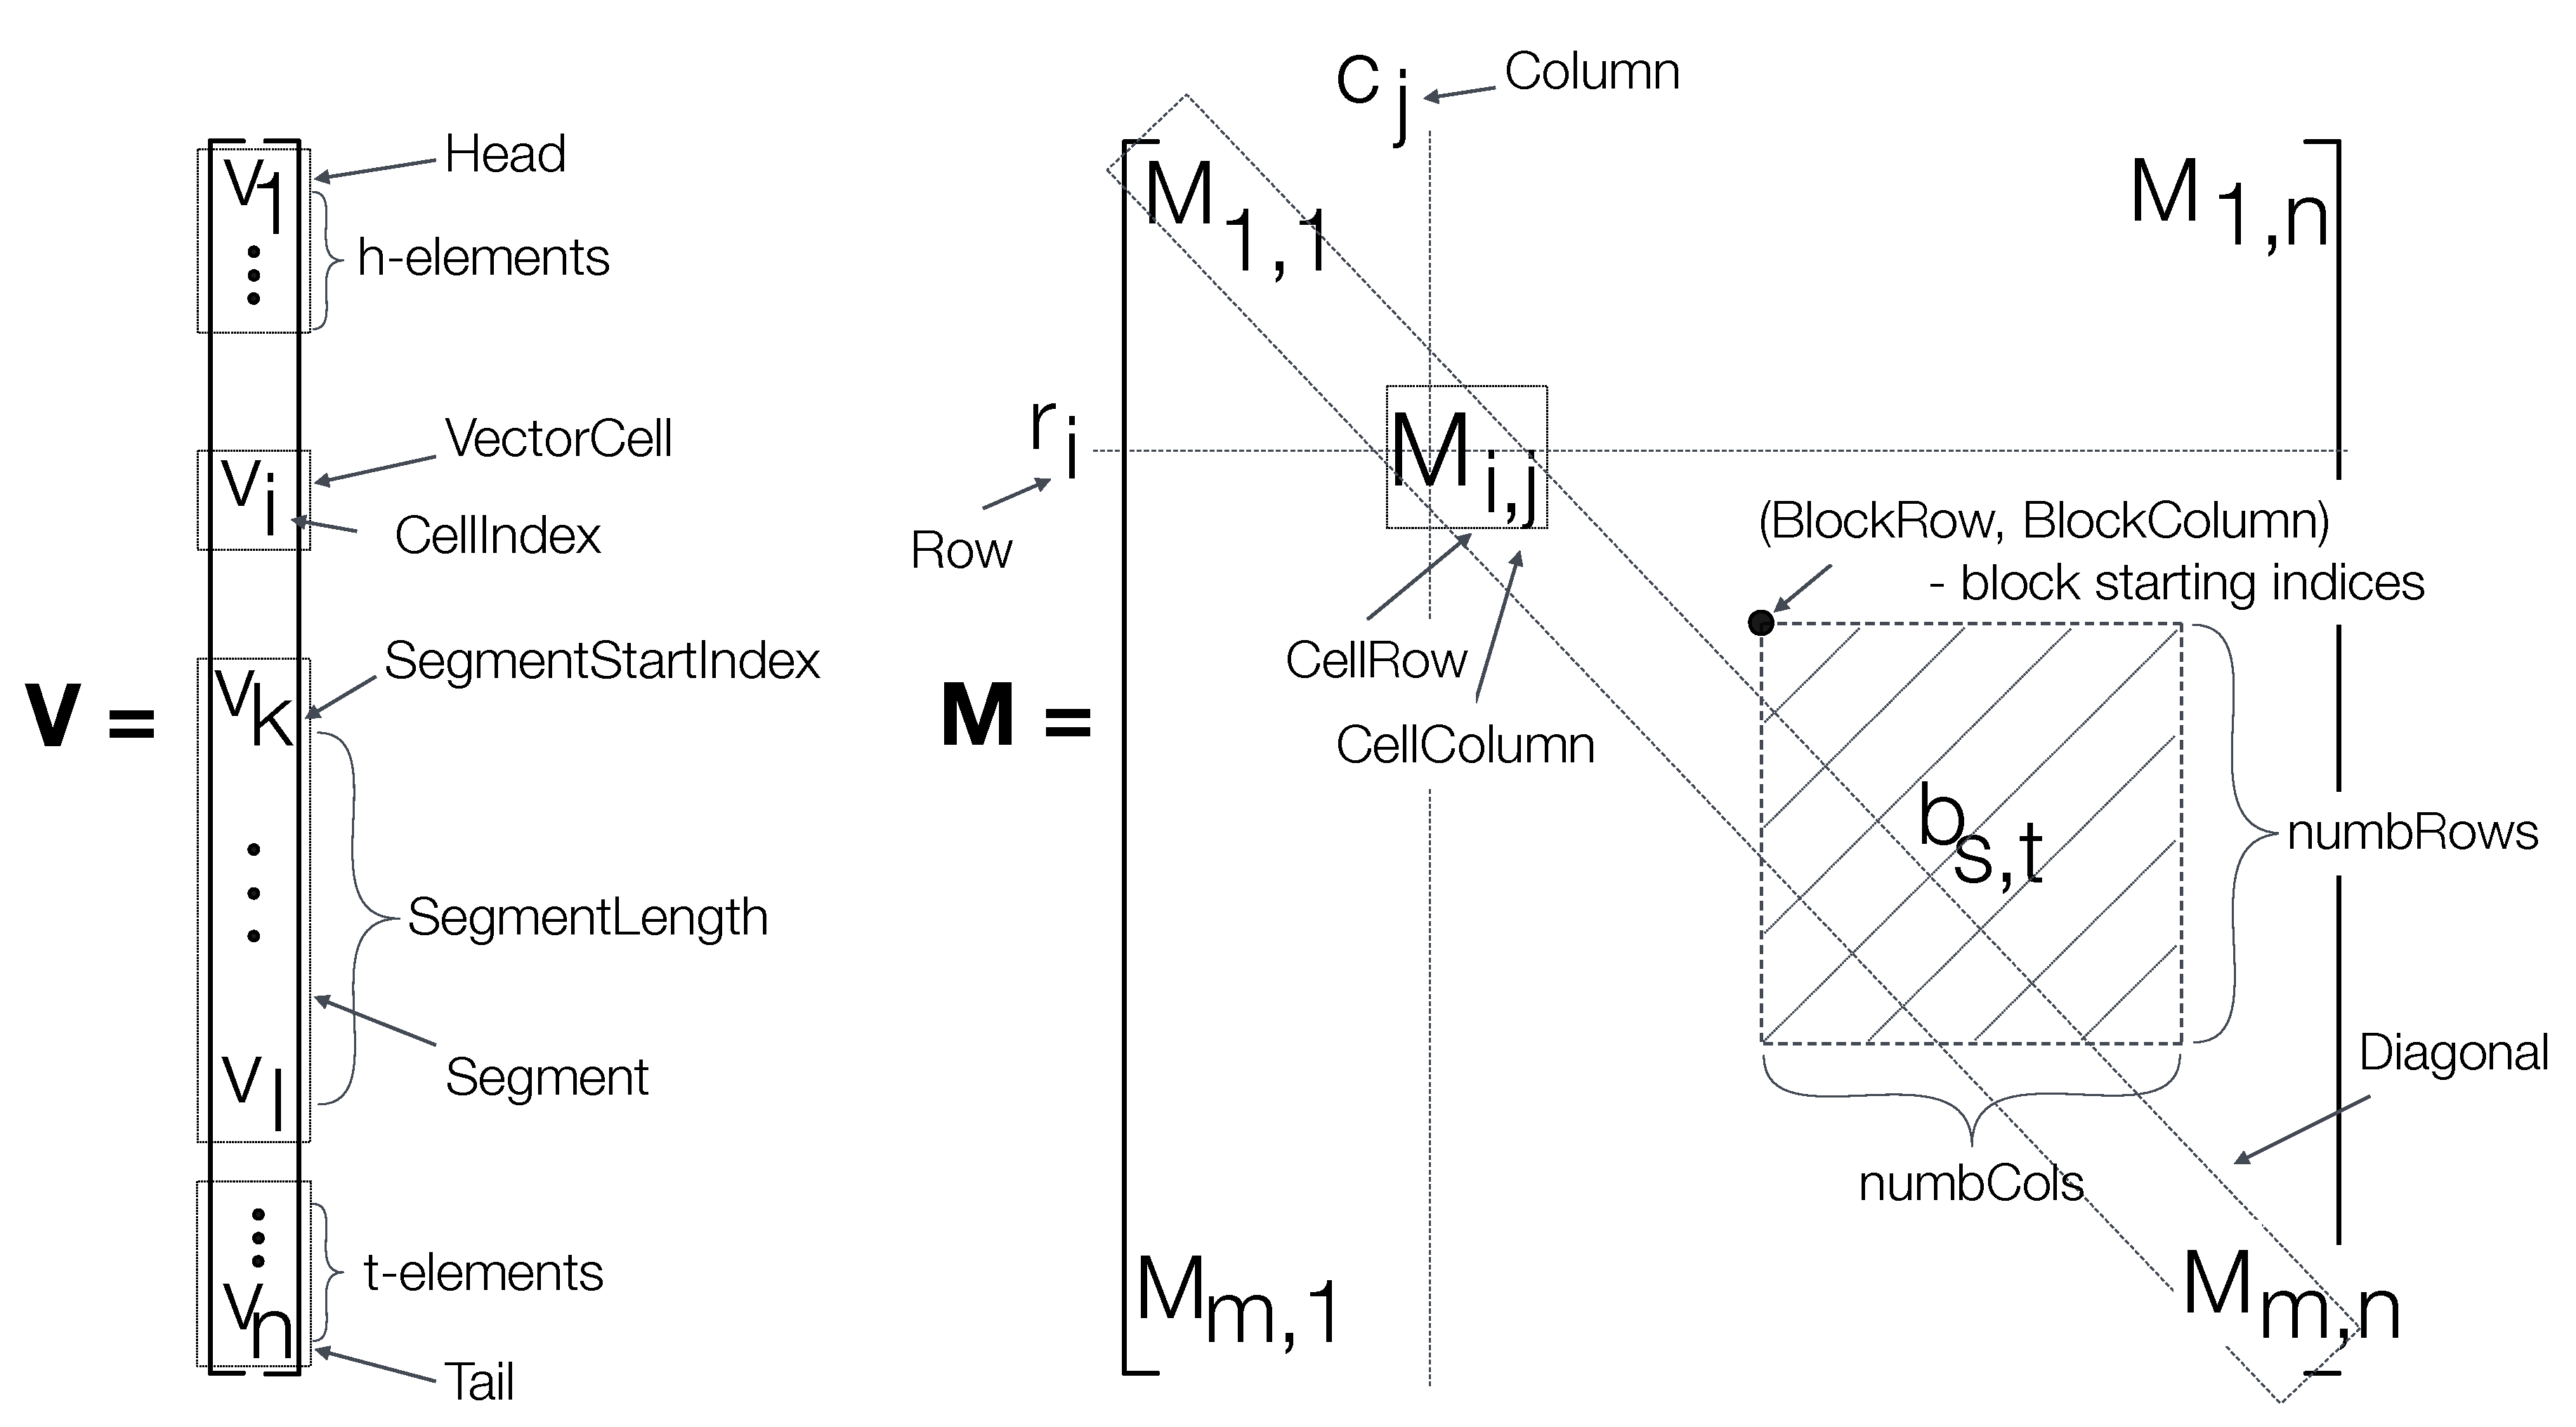
\includegraphics[width=170mm]{pics/VectorMatrixStructure}
\caption{Vector and matrix -- vocabulary and structure overview.}
\label{fig:vectorMatrix}
\end{figure}



%%%%%%%%%%%%%%%%%%%%%%%%%%%%%%%%%%%%%%%%%%%%%%%%%%%%%%%%%%%%%%%%%%%%%%
\subsection{Vector structure with examples}
\label{subsec:vectorType}
The index for vector or matrix elements start with 1. Vectors are assumed to 
be column vectors. We provide both support for populating and reading 
vectors. 

\subsubsection{Populating vectors}
The elements and attributes that are available to handle most common situation,
schematically visualised in Figure \ref{fig:vectorMatrix} (left).

Table \ref{tab:twoOptionsForVector} shows two examples of how a sparse vector 
[0,2,0,0,5,0,0,0,0,0] can be coded in \pharmml. A vector is either 
encoded explicitly with \xelem{VectorElements} using a mixture of numbers 
and symbol references or using the \xelem{VectorCell} elements (bottom right). 
The latter option, allowing to avoid unnecessary repetitions, requires the 
\xatt{default} attribute to define all remaining entires and \xatt{length} attribute 
to infer the vector length.

\begin{table}[hb!]
\setlength{\tabcolsep}{5pt}
\begin{center}
\begin{tabular}{ll}
  \hline
 Population of a vector using  	& Populating a vector using \xelem{VectorCell} \\
 \xelem{VectorElements}		& and attributes \xatt{default} and \xatt{length} \\
  \hline
\lstset{language=XML}
\begin{lstlisting}
<SimpleParameter symbId="V1">
    <ct:Assign>
        <ct:Vector length="10">
            <ct:VectorElements>
                <ct:Real>0</ct:Real>
                <ct:Real>2</ct:Real>
                <ct:Real>0</ct:Real>
                <ct:Real>0</ct:Real>
                <ct:SymbRef symbIdRef="fifthElement"/>
                <ct:Real>0</ct:Real>
                <ct:Real>0</ct:Real>
                <ct:Real>0</ct:Real>
                <ct:Real>0</ct:Real>
                <ct:Real>0</ct:Real>
            </ct:VectorElements>
        </ct:Vector>
    </ct:Assign>
</SimpleParameter>
\end{lstlisting}  
    &
    \lstset{language=XML}
    \begin{lstlisting}
<SimpleParameter symbId="V2">
    <ct:Assign>
        <ct:Vector default="0" length="10">
            <ct:VectorCell>
                <ct:CellIndex>
                    <ct:Int>2</ct:Int>
                </ct:CellIndex>
                <ct:Real>2</ct:Real>
            </ct:VectorCell>
            <ct:VectorCell>
                <ct:CellIndex>
                    <ct:Int>5</ct:Int>
                </ct:CellIndex>
                <ct:SymbRef symbIdRef="fifthElement"/>
            </ct:VectorCell>
        </ct:Vector>
    </ct:Assign>
</SimpleParameter>
    \end{lstlisting} 
    \\
    \hline
\end{tabular}
\caption{Comparison of two encoding types of the vector [0,2,0,0,5,0,0,0,0,0].
The vector is either encoded explicitly with \xelem{VectorElements} using a mixture 
of numbers and symbol references (left) or using the \xelem{VectorCell} elements (right).
In the latter case the use of attributes  \xatt{default} and \xatt{length} is required,
otherwise the dimension of the vector could not be estimated.}
\label{tab:twoOptionsForVector}
\end{center}
\end{table}


\subsubsection{Reading vectors}
Selecting elements out of a vector is very flexible and efficient. 
Once a vector is assigned, we need a mechanism for the readout of vector
elements. This is done with the \xelem{VectorSelector} element. 
Let's consider following basic assignment operation
\begin{align}
	& m = a + V2[5] \nonumber
\end{align}
i.e. adding parameter $a$ to the fifth element of vector $V2$. 
The following code shows how this is done. 

\lstset{language=XML}
\begin{lstlisting}
           <SimpleParameter symbId="m">
               <ct:Assign>
                   <math:Equation>
                       <math:Binop op="plus">
                           <ct:SymbRef symbIdRef="a"/>
                           <ct:VectorSelector>
                               <ct:SymbRef symbIdRef="V2"/>
                               <ct:Cell>
                                   <ct:Int>5</ct:Int>
                               </ct:Cell>
                           </ct:VectorSelector>
                       </math:Binop>
                   </math:Equation>
               </ct:Assign>
           </SimpleParameter>
\end{lstlisting}

Additionally to the vocabulary we used before, we have now the \xelem{Head} and \xelem{Tail} 
methods, i.e. two ways to extract the first or last $n$ elements which number can be specified
explicitly. The following child elements allow flexible access to any vector element: 
\xelem{SymbRef} identifies the vector of interest (mandatory), 
\xelem{Cell} is used to pick one element, and
\xelem{Segment} allows to select a segment of a vector.


Assume a vector V2 that has 13 elements and we want to select only those specified by the
following indexes $i=\{1:3,\;6:8,\;10,\;12:13\}.$
\lstset{language=XML}
\begin{lstlisting}
            <SimpleParameter symbId="n">
                <ct:Assign>
                    <math:Equation>
                        <ct:VectorSelector>
                            <ct:SymbRef symbIdRef="V2"/>
                            <ct:Head><ct:Int>3</ct:Int></ct:Head>
                            <ct:Segment>
                                <ct:StartIndex><ct:Int>6</ct:Int></ct:StartIndex>
                                <ct:SegmentLength><ct:Int>3</ct:Int></ct:SegmentLength>
                            </ct:Segment>
                            <ct:Cell><ct:Int>10</ct:Int></ct:Cell>
                            <ct:Tail><ct:Int>2</ct:Int></ct:Tail>
                        </ct:VectorSelector>
                    </math:Equation>
                </ct:Assign>
            </SimpleParameter>
\end{lstlisting}


%%%%%%%%%%%%%%%%%%%%%%%%%%%%%%%%%%%%%%%%%%%%%%%%%%%%%%%%%%%%%%%%%%%%%%
\subsection{Matrix structure with examples}
\label{subsec:matrixStructure}
Similarly to the vector structure there are a few alternative options to encode a matrix.
Note, that for now matrices can be used for encoding of the correlation structure between\marginpar{COMPLETE DESCRIPTION AND SECTION} 
random effect, i.e. within the \xelem{Correlation} element only. Their use will be extended to 
handle covariance matrices of multivariate distributions and other model elements in 
a future release. The index for matrix elements start with 1.

\subsubsection{Populating matrices}
\pharmml provides multiple ways to populate matrices. 
Following matrix, $\Sigma$ can be represented as a full matrix or sparse matrix. 
\label{subsec:matrixType}
\begin{align}
\Sigma = 
  \begin{bmatrix} 
  1 & \Sigma_{12} & 0 & 0 \\
  0 & 1 & \Sigma_{23} & 0 \\
  \Sigma_{31} & 0 & 1 & 0 \\
  0 & 0 & 0 & \Sigma_{44} \nonumber \end{bmatrix} 
\end{align}

\subsubsection{Implementation of $\Sigma$ as full matrix}
This is a straightforward implementation of every matrix element explicitly using
the \xelem{MatrixRow} elements, which is used to define the matrix row-by-row.  
\lstset{language=XML}
\begin{lstlisting}
            <Correlation deviationMatrixType="CovMatrix">
                <ct:VariabilityReference>
                    <ct:SymbRef symbIdRef="indiv"/>
                </ct:VariabilityReference>
                <Matrix matrixType="Any">
                    <ct:MatrixRow>
                        <ct:RowIndex><ct:Int>1</ct:Int></ct:RowIndex>
                        <ct:Real>1</ct:Real>
                        <ct:SymbRef symbIdRef="Sigma12"/>
                        <ct:Real>0</ct:Real>
                        <ct:Real>0</ct:Real>
                    </ct:MatrixRow>
                    <!-- omitted rows 2 & 3 -->
                    <ct:MatrixRow>
                        <ct:RowIndex><ct:Int>4</ct:Int></ct:RowIndex>
                        <ct:Real>0</ct:Real>
                        <ct:Real>0</ct:Real>
                        <ct:Real>0</ct:Real>
                        <ct:SymbRef symbIdRef="Sigma44"/>
                    </ct:MatrixRow>
                </Matrix>
            </Correlation> 
\end{lstlisting}
 
\subsubsection{Implementation of $\Sigma$ as sparse matrix}
Here the $\Sigma$ matrix is implemented using \xelem{MatrixCell}, which is useful for matrices with a few non-zero elements. Only four 
values have to be stored while the rest is encoded using \xatt{diagDefault} and \xatt{offDiagDefault} attributes.
\lstset{language=XML}
\begin{lstlisting}
            <Correlation deviationMatrixType="CovMatrix">
                <ct:VariabilityReference>
                    <ct:SymbRef symbIdRef="indiv"/>
                </ct:VariabilityReference>
                <Matrix matrixType="Any" diagDefault="1" offDiagDefault="0">
                    <ct:MatrixCell>
                        <ct:CellRow><ct:Int>1</ct:Int></ct:CellRow>
                        <ct:CellColumn><ct:Int>2</ct:Int></ct:CellColumn>
                        <ct:SymbRef symbIdRef="Sigma12"/>
                    </ct:MatrixCell>
                    <!-- omitted MatrixCell's in rows 2 & 3 -->
                    <ct:MatrixCell>
                        <ct:CellRow><ct:Int>4</ct:Int></ct:CellRow>
                        <ct:CellColumn><ct:Int>4</ct:Int></ct:CellColumn>
                        <ct:SymbRef symbIdRef="Sigma44"/>
                    </ct:MatrixCell>
                </Matrix>
            </Correlation>
\end{lstlisting}  
Note that the attributes \xatt{diagDefault} and \xatt{offDiagDefault}
are set to 1 or 0, respectively, which makes the matrix encoding very efficient.

\subsubsection{Example 1 -- Covariance matrix with expressions}
The elements of a matrix can contain arbitrary expressions. For example, the following covariance matrix
\begin{align}
\Sigma = 
  \begin{bmatrix} 
  	\sigma_V^2  			& \rho\; \sigma_V \sigma_k \\
        \rho\; \sigma_V \sigma_k   	& \sigma_V^2 \nonumber \\
\end{bmatrix} 
\end{align}
is easily implemented as the following code shows

\lstset{language=XML}
\begin{lstlisting}
            <Correlation deviationMatrixType="CovMatrix">
                <ct:VariabilityReference>
                    <ct:SymbRef blkIdRef="modelVar" symbIdRef="indiv"/>
                </ct:VariabilityReference>
                <Matrix matrixType="Any">
                    <ct:MatrixRow>
                        <ct:RowIndex><ct:Int>1</ct:Int></ct:RowIndex>
                        <math:Equation>
                            <math:Binop op="power">
                                <ct:SymbRef symbIdRef="sigma_V"/>
                                <ct:Real>2</ct:Real>
                            </math:Binop>
                        </math:Equation>
                        <math:Equation>
                            <math:Binop op="times">
                                <ct:SymbRef symbIdRef="rho"/>
                                <math:Binop op="times">
                                    <ct:SymbRef symbIdRef="sigma_V"/>
                                    <ct:SymbRef symbIdRef="sigma_k"/>
                                </math:Binop>
                            </math:Binop>
                        </math:Equation>
                    </ct:MatrixRow>
                    <!-- omitted 2nd row -->
                </Matrix>
            </Correlation>
\end{lstlisting}  


%%%%%%%%%%%%%%%%%%%%%%%%%%%%%%%%%%%%%%%%%%%%%%%%%%
\subsubsection{Reading matrices}
Once a matrix is assigned, we need a mechanism for the readout of its elements. 
This is done with the \xelem{MatrixSelector} element. 
Following code shows few examples of how to access single element or 
row from the $\Sigma$ matrix defined in previous example.

\lstset{language=XML}
\begin{lstlisting}
            <!-- extract one element -->
            <SimpleParameter symbId="rho_tlag_ka">
                <ct:Assign>
                    <math:Equation>
                        <ct:MatrixSelector>
                            <ct:SymbRef symbIdRef="Omega"/>
                            <ct:Cell>
                                <ct:RowIndex><ct:Int>1</ct:Int></ct:RowIndex>
                                <ct:ColumnIndex><ct:Int>2</ct:Int></ct:ColumnIndex>
                            </ct:Cell>
                        </ct:MatrixSelector>
                    </math:Equation>
                </ct:Assign>
            </SimpleParameter>
            
            <!-- extract 2nd row -->
            <ct:Variable symbolType="real" symbId="SecondRow">
                <ct:Assign>
                    <math:Equation>
                        <ct:MatrixSelector>
                            <ct:SymbRef symbIdRef="Omega"/>
                            <ct:Row>
                                <ct:Int>2</ct:Int>
                            </ct:Row>
                        </ct:MatrixSelector>
                    </math:Equation>
                </ct:Assign>
            </ct:Variable>
\end{lstlisting}


\section{Representing statistics}

As can be seen in chapter \ref{chap:mathsdefn}, \pharmml relies on the
ability to use probability distributions to describe the variability
in a pharmacometric model. Admittedly, the most commonly used
distribution is the normal distribution (or transformations of it),
but our intention is that \pharmml will have the flexibility to
describe a wide range of probability distribution types. To do this
the languages uses \uncertml version
3\footnote{\url{http://www.uncertml.org}}, which is an XML Schema
based language that aims to ``describe and exchange
uncertainty''. UncertML supports all the commonly used continuous and
discrete probability distributions and so more than adequately
supports the needs of \pharmml.  As an example we can show how the
normal distribution $\mathcal{N}(0, \omega^2)$ can be defined in
\uncertml.
% shown in listing \ref{code:normal-dist-eg}.
\lstset{language=XML}
\begin{lstlisting}
<NormalDistribution xmlns="http://www.uncertml.org/3.0"
    definition="http://www.uncertml.org/distributions/normal">
    <mean>
        <rVal>0</rVal>
    </mean>
    <stddev>
        <var varId="omega"/>
    </stddev>
</NormalDistribution>
\end{lstlisting}

% \begin{listing*}[htb]
% \inputxml{normal.xml}
% \caption{XML code encoding the normal distribution, $\mathcal{N}(0,
%   1)$.}
% \label{code:normal-dist-eg}
% \end{listing*}


% \section{Representing the Structural Model}

% In \pharmml one of our aims has been to reuse existing standards where it
% makes sense to do so. One standard that is suited for this purpose is
% \sbml. It can be used to encode systems of ODEs or algebraic
% equations, but it can also encode more complicated mechanistic models
% too. For example models that describe signalling pathways spanning
% multiple compartment. Therefore, it is our preferred mechanism for
% representing the structural model in \pharmml.

% However, in order to use a structural model encoded in \sbml we need
% to somehow incorporate it into the \pharmml document. We do this with the
% \xelem{Import} element as can be seen in listing
% \ref{code:import-eg}. In doing so the import statement maps equivalent
% variables in the \pharmml document to those in the \sbml model.

% \begin{listing*}[htb]
% \inputxml {sbml-import1.xml}
% \caption{This snippet illustrates how we map the parameters
%   and variables in the \pharmml document to the \sbml model. The model
%   itself is identified by a URL and the type of model is identified as
% \attval{sbml}. The variables and the parameters (not shown) in the
% \pharmml document are mapped to those in the \sbml model.}
% \label{code:import-eg}
% \end{listing*}

% In addition to incorporating \sbml models we can also incorporate
% other structural models defined in \pharmml. This mechanism is there for
% completeness and is not the preferred method for including models,
% so we will not go into in more detail here.

\section{Time}
\label{sec:independent-var}

Time is required by most pharmacometric models and in \pharmml it can
be referred to explicitly. The symbol used for the time variable is
configurable at the beginning of the document as shown below:

\lstset{language=XML}
\begin{lstlisting}
<PharmML xmlns="http://www.pharmml.org/pharmml/0.6/PharmML"
    xmlns:xsi="http://www.w3.org/2001/XMLSchema-instance"
    xsi:schemaLocation="http://www.pharmml.org/pharmml/0.6/PharmML ..."
    xmlns:math="http://www.pharmml.org/pharmml/0.6/Maths"
    xmlns:ct="http://www.pharmml.org/pharmml/0.6/CommonTypes"
    xmlns:ds="http://www.pharmml.org/pharmml/0.6/Dataset"
    xmlns:design="http://www.pharmml.org/pharmml/0.6/TrialDesign"
    writtenVersion="0.6">
    <ct:Name>IOV1 with covariates</ct:Name>
    <IndependentVariable symbId="t"/>
\end{lstlisting}

Rather than time we call the element \xelem{IndependentVariable}
because this is more correct and because you could define a model that
uses another quantity than time as the independent variable (e.g.\xspace
dose in a dose-response model). Note that the independent variable
always has a real type.

\section{Element identifier}
\label{sec:element-id}

To enable other resources to refer to
specific pieces of information in a \pharmml document,
every XML element in the document with an optional unique
identifier is provided. The listing below shows how the \xatt{id} attribute is
used:
%
\lstset{language=XML}
\begin{lstlisting}
<FixedEffect id="e10" symbId="beta_V">
    <Covariate>
        <ct:SymbRef  symbIdRef="W"/>
    </Covariate>
</FixedEffect>
<FixedEffect id="e13" symbIdRef="beta_Cl">
    <Covariate>
        <ct:SymbRef symbIdRef="W"/>
    </Covariate>
</FixedEffect>
<RandomVariable id="e16" symbId="eta_V">
    <ct:VariabilityReference id="e17">
        <ct:SymbRef id="e18"  blkIdRef="model" symbIdRef="level"/>
   </ct:VariabilityReference>
   <!-- Snip -->
</RandomVariable>
\end{lstlisting}
%
The \xatt{id} attribute is optional and need only be
used for elements that you want to refer to. There are no rules other
than that the identifier must be unique within the \pharmml document.
Thus to refer to a specific part of a document all you need to define is
the location of the document and the identifier. So assuming that the
above code snippet is found in a file called ``testFile.xml'' a
suitable (relative) URI that refers to the random variable in the
example might be \url{testFile.xml#e16}.

The benefit of this approach is that the \xatt{id} attribute can
easily be made available programmatically and searched on with a class
library generated from the XML Schema.
%\footnote{We considered using the XPath
% standard\cite{xpath} to identify elements using what is in effect an
% XMl query language, but we felt that it would be very difficult to
% execute such queries on a class library encode in a programming
% language the query is on the XML not attributed help within the prograsuch as
% Java, which is what you would need to do when interacting with
% \pharmml via the libPharmML API (see section
% \ref{sec:libpharmml}).
This mechanism is also used successfully by SBML \cite[Section
6]{sbmll3v1c}. You will see in the sections below (sections \ref{sec:annotation} and
\ref{sec:extension}) how we take advantage of this mechanism to
annotate and extend a \pharmml document.

\section{Ordering modelling steps}

Descriptions in a modelling step are declarative, describing what
was done, what algorithms were used and what their properties were.

\begin{figure}[htb]
 \centering
  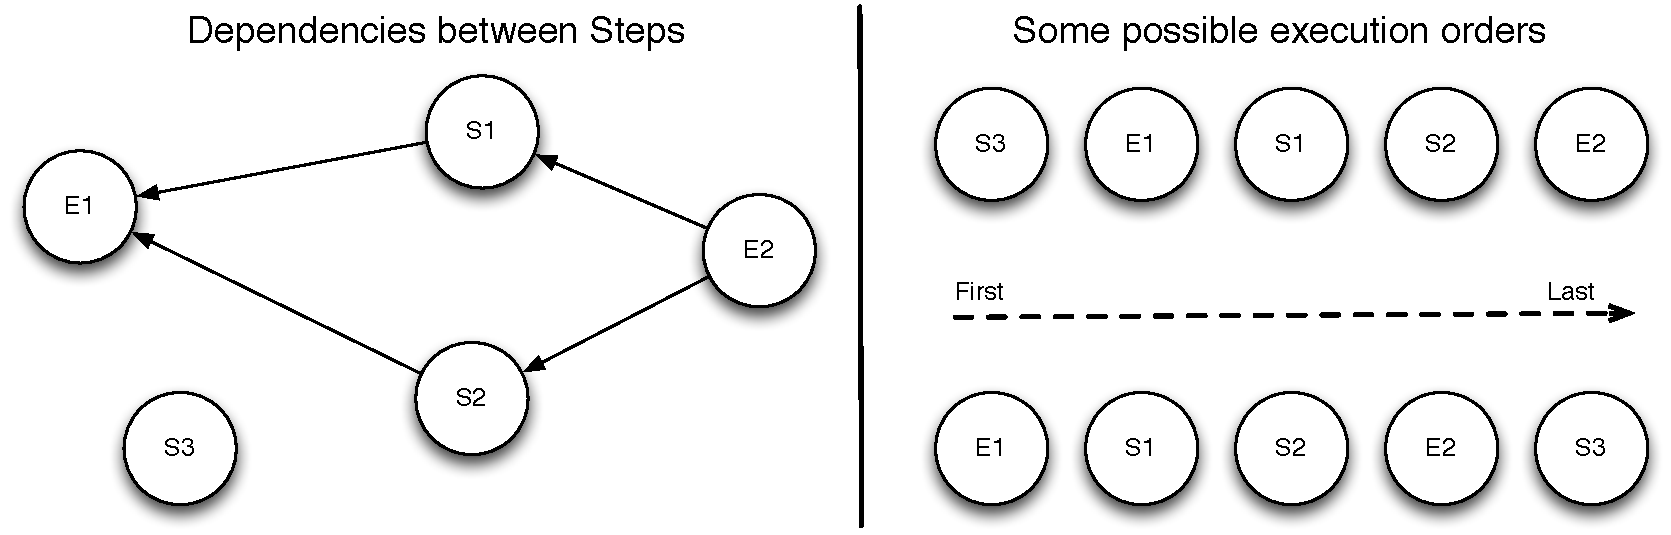
\includegraphics[width=1\linewidth]{Figures/ModellingStepDeps}
  \caption{An example of the dependencies between modelling steps is
    shown on the left. The arrow indicates the direction of the
    dependency so step S1 is dependent on the successful completion of
    step E1. So in this example step E1 must be executed before step
    S1 and S2, and those steps must both execute before step E2. On
    the right-hand figure we show two possible execution orders that
    correspond to the task dependecies on the left. It is important to
    remember that, as in this example, there can be more than one
    execution order for a given set of task dependencies.}
  \label{fig:modellingstep_deps}
\end{figure}

The \emph{Modelling Steps} section has two components that describe
simulation or estimation tasks. Multiple tasks can be linked together so
that a given estimation task can be placed before a given simulation
task or no order can be given in which case tasks can be executed in
parallel or in any order. A task is ordered by defining its dependent
tasks: tasks that must complete successfully before it can start (see
figure~\ref{fig:modellingstep_deps}). In this way the modelling steps
make no assumptions about how or where its tasks are executed, but
provides enough information for a workflow engine to parallelise the
execution of its tasks successfully, should it wish to.

At the moment tasks cannot specify how output is generated from either
an Estimation or Simulation step. A result of this restriction is that
it is \emph{not} possible to exchange information from one modelling
step to another: for example to use the output of an estimation to set
the parameter values in an estimation. We recognise that this is a
limitation of the current version and this functionality will be
provided in a future release of \pharmml.


\section{Supporting Resources}
\label{sec:supporting-res}

\subsection{Metadata: annotating the \pharmml document}
\label{sec:annotation}

As has been stated in Chapter \ref{chap:scope}, the purpose of
the \pharmml document is to provide a mathematical and structural
description of a pharmacometric model, sufficient for it to be
executed. Additional information, such as a description of the disease
process being modelled, the exact estimation algorithm or a
publication describing the model is not included in the \pharmml
document. Typically called metadata, this information is very 
important and \pharmml provides support for external annotation.

\begin{figure}[htbp]
\centering
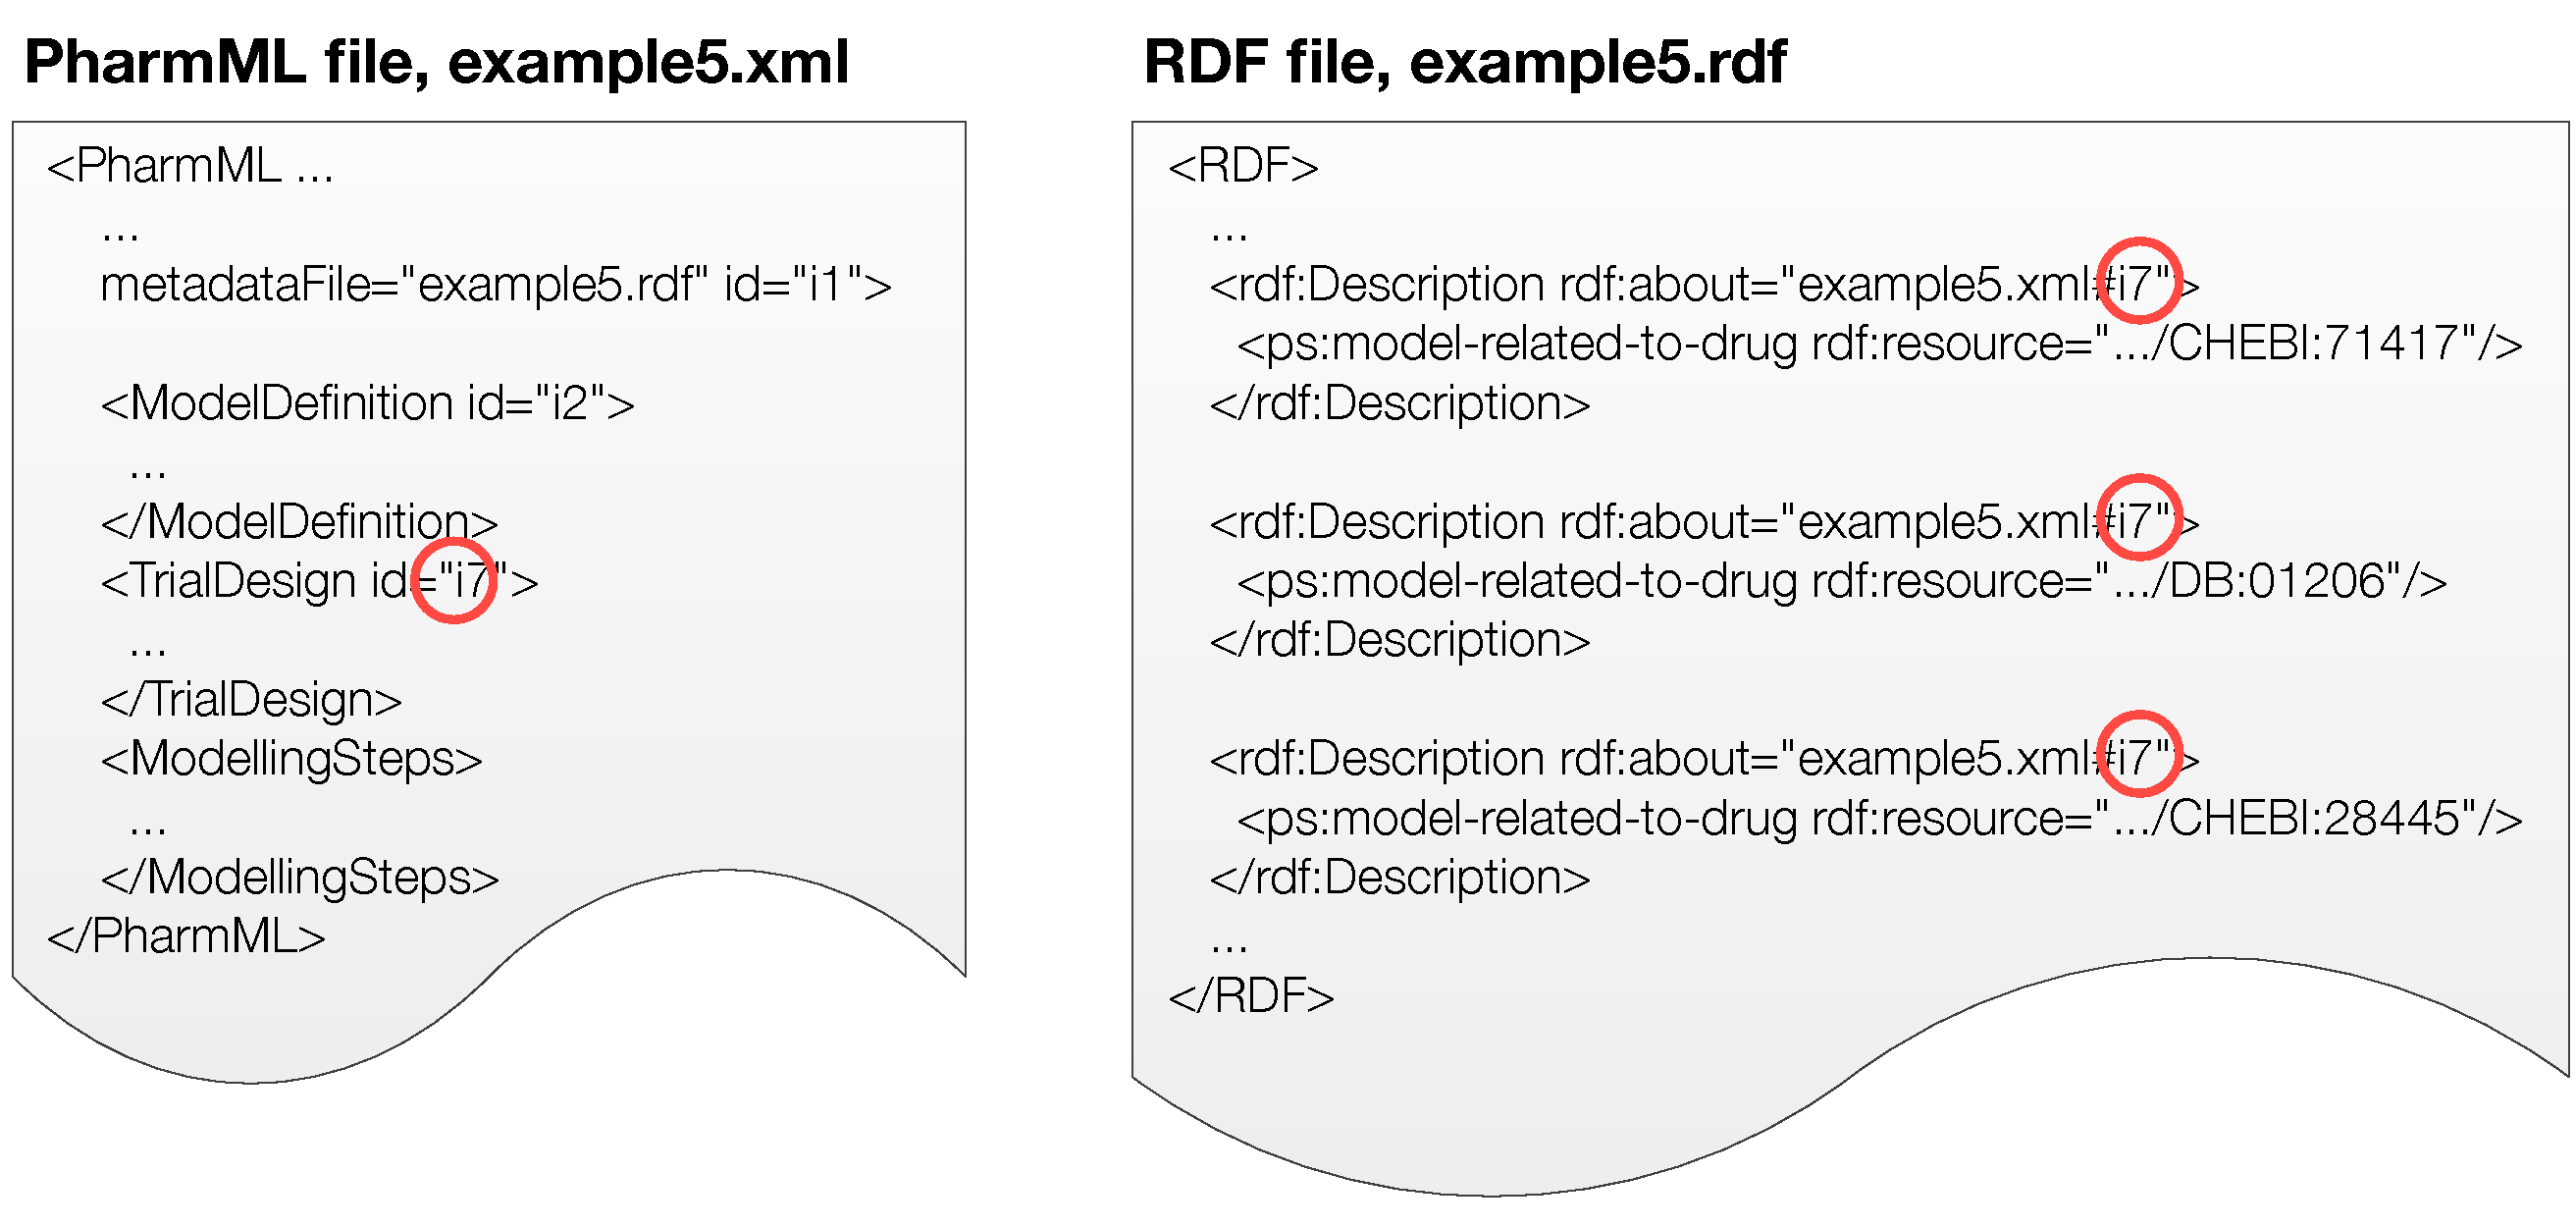
\includegraphics[width=0.8\linewidth]{pics/PharmML_RDF.pdf}
\caption{On schematic overview of the \pml, \emph{example5.xml} and RDF, 
\emph{example5.rdf}, files relationships. Note, that we use here, for the sake of clarity, 
a simplified RFD statements. See the code snippet at the end of this section 
for the correctly formatted RDF file \cite{RDF_1.1}.}
\label{fig:pharmmlRdf}
\end{figure}

We expect such metadata comes in the form of ontological annotation and
while the detail of what will be annotated is out of scope of this
document it is important to stress that every \pml element can be annotated. 
This is done by adding an attribute, e.g. \xatt{id="i7"}, to the \xelem{TrialDesign}
element, see Figure \ref{fig:pharmmlRdf}.\footnote{More information on 
annotating \pharmml models are described in the \pharmml Metadata Specification.} 
The following example gives you a flavour of what an RDF annotation of 
a \pharmml document would look like. 
The metadata above is encoded in RDF-XML, \cite{RDF_1.1},
and annotates 3 external terms; CHEBI:71417, DB01206, and CHEBI:28445.

\begin{figure}[htbp]
\centering
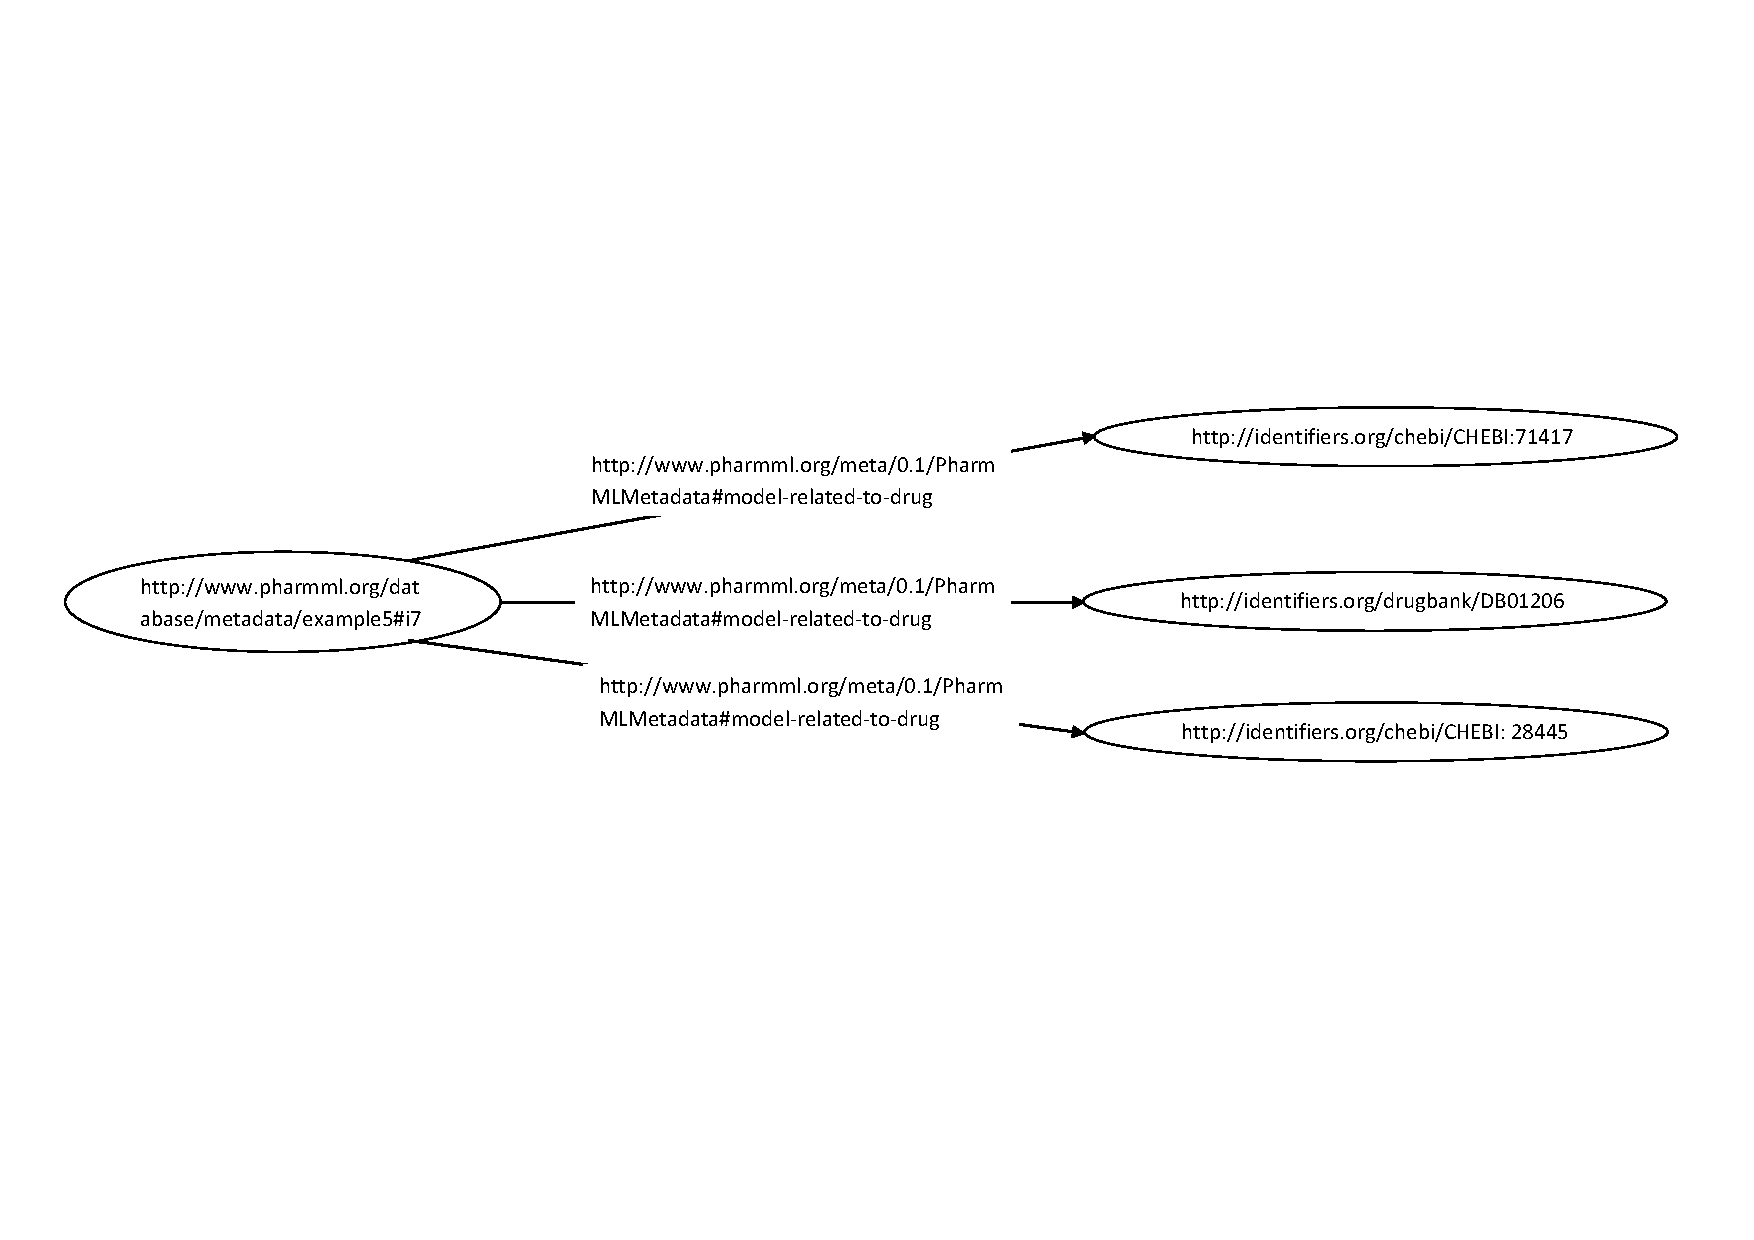
\includegraphics[width=0.95\linewidth]{pics/metadatadiagram.pdf}
\caption{This figure illustrates how information in the RDF example is
organised. Simply put the subject of the annotation is on the left and
is annotated by the object on the right. The meaning of that
annotation is described by the \emph{predicate} term labelling the
arrow. So reading the top subject from left to right we understand that
element assigned the attribute \xatt{i7} is \emph{model-related-to-drug} at \emph{CHEBI:71417}.}
\label{fig:rdf-graph}
\end{figure}
This is a basic example, but it illustrates how the \pharmml document can be annotated 
using metadata described in a separate RDF document

%
\lstset{language=XML}
\begin{lstlisting}
<rdf:RDF
    xmlns:rdf="http://www.w3.org/1999/02/22-rdf-syntax-ns#"
    xmlns:rdfs="http://www.w3.org/2000/01/rdf-schema#"
    xmlns:base="http://www.pharmml.org/database/metadata/example5#"
    xmlns:example5="http://www.pharmml.org/database/metadata/example5#"
    xmlns:ps="http://www.pharmml.org/meta/0.1/PharmMLMetadata#"> 
    
    <rdf:Description rdf:about="#i7">
        <ps:model-related-to-drug rdf:resource="http://identifiers.org/chebi/CHEBI:71417"/>
        <ps:model-related-to-drug rdf:resource="http://identifiers.org/drugbank/DB01206"/>
        <ps:model-related-to-drug rdf:resource="http://identifiers.org/chebi/CHEBI:28445"/>
    </rdf:Description>
</rdf:RDF>
\end{lstlisting}

\subsection{Extending PharmML}
\label{sec:extension}

As with any standard there will be circumstances when it does not
represent all the information that you would like and it would be
convenient to extend it. Typically there are two scenarios where this
is likely to be the case. The first is when the information is genuinely
not supported by \pharmml. This may be because it has not been
implemented yet, or it may be that there is no consensus about whether
this information should be included or no agreement about the best way
to represent it. The second scenario is when you want to
add application specific information to a \pharmml document. Perhaps
because a tool wishes to use \pharmml as its native storage format in
which case it would also want to store information about application
settings etc.

Whatever the reason \pharmml can be extended. Like the metadata
descriptions above (section \ref{sec:annotation}) this approach relies
on the element identifier (see section~\ref{sec:element-id}). The
recommended approach is that you develop a separate XML document
(typically in a separate file), which we will call the extension
document, using any XML representation you choose. Where information
in the extension document relates to the content of the \pharmml
document then you can refer to the relevant XML element using its
identifier.

\begin{figure}[htb]
\centering
  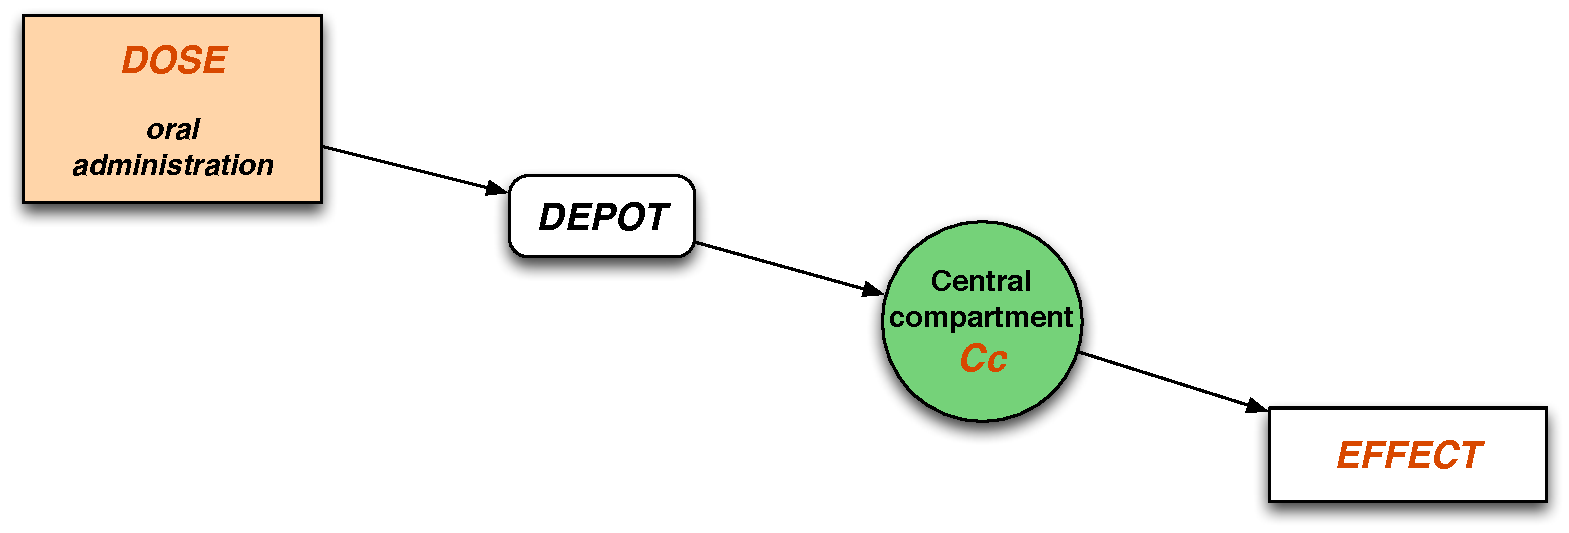
\includegraphics[height=0.2\textheight]{Figures/GraphicalModel}
  \caption{This diagram is reproduced from an example in the Monolix
    user manual \cite{Monolix4.1.4UserGuide:2012} and it provides a
    graphical description of a structural model. In the hypothetical
    example in the text we illustrate how you might extend \pharmml to
    link this graphic with the components of the model it represents.}
\label{fig:graphical-model}
\end{figure}

We can illustrate with an example based on the second scenario we
described above: application specific extensions. In this scenario our
software tool provides a graphical interface that lets you create a
pharmacometric model by drawing and connecting shapes such as the
diagram in figure~\ref{fig:graphical-model}. When you save the diagram
the application saves both the \pharmml that encodes the model and an
extension document that describes the graphical layout and maps the
graphical elements to the relevant parts of the model. The extension
document could look like this:
%
\lstset{language=XML}
\begin{lstlisting}
<Diagram resource="file:///anotherPharmMLFile.xml">
    <Rectangle id="1">
        <Name>Dose</Name>
        <Bounds x="10" y="10" w="50" h="30"/>
        <!-- Omitted other information such as colour and other text-->
        <Ref idRef="e35"/>
    </Rectangle>
    <!-- Omitted -->
    <Circle id="3">
        <Name>Central</Name>
        <Bounds x="10" y="200" w="45" h="45"/>
        <!-- Omitted other information such as colour and other text-->
        <Ref idRef="e46"/>
    </Circle>
    <!-- Omitted other shape definitions-->
    <Link src="1" tgt="2"/>
    <Link src="2" tgt="3"/>
    <Link src="3" tgt="4"/>
</Diagram>
\end{lstlisting}
%
The XML describes the shapes of the nodes, their location and the
connections between them. What allows it to extend the \pharmml document?
First the \xatt{resource} attribute provides a URL describing
the location of the \pharmml document being extended. Next the
\xelem{Ref} element defines a reference that points to an element in
the \pharmml document. From this information the application is able
to read both the \pharmml and the extension documents and then relate
the diagram to the relevant part of the model.

Note that while this is a hypothetical example for \pharmml, this type
of solution has been implemented by a graphical Systems Biology editor
called CellDesigner\footnote{\url{http://www.celldesigner.org}}. It uses SBML
as its native application format: encoding the model in SBML and using
SBML's extension facilities to store graphical information and other
application specific properties.

One final clarification. The extension mechanism does not require an
application to use the same XML elements as described in the example
above. The XML content of the extension document is entirely the
concern of the application. In order to extend a \pharmml document
all it must do is:
\begin{enumerate}
\item Specify how to find the \pharmml document. Using a URI is a good
  way to do this.
\item Use the element identifier to refer to the content of the \pharmml document.
\end{enumerate}

\subsection{Organising \pharmml resources}
\label{sec:pharmml-archive}

We expect that \pharmml will in normal usage consist of more than one
file. From the discussion about annotating
(section~\ref{sec:annotation}) and extending
(section~\ref{sec:extension}) \pharmml it is clear that both of these
cases require the creation of resources that are closely
related to a \pharmml document. It is therefore desirable that they
are kept together and exchanged and used together.

\begin{figure}[htb]
\centering
  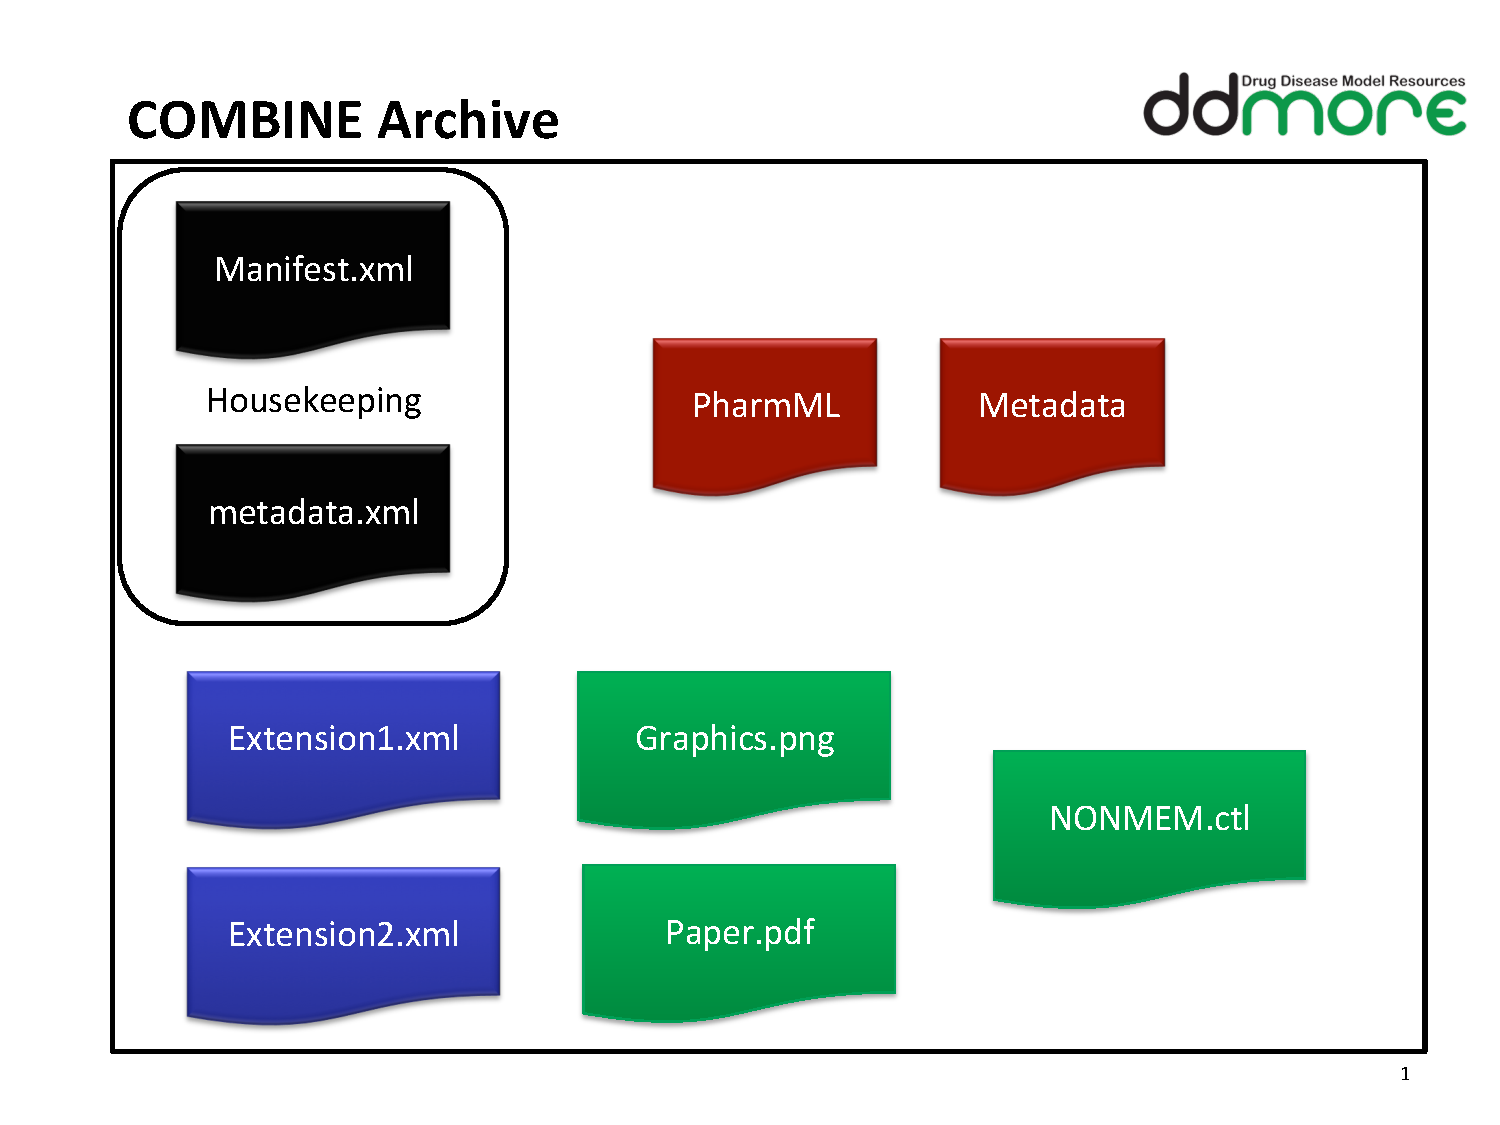
\includegraphics[width=0.6\textwidth]{Figures/AchiveOverview}
  \caption{An overview of how a COMBINE archive may be used to hold
    XML documents and files associated with a model encoded in
    \pharmml. In this example the archive holds the model and its
    metadata (in red) and two application specific extension
    documents (in blue). This also shows another advantage of using
    the archive: you can store other useful information, such as the
    original model file, relevant papers or images (in
    green). Finally, the archive contains a metadata file (in black)
    that helps an application reading the archive make sense of what
    it contains.}
  \label{fig:moml-archive-overview}
\end{figure}

An archive file can provide this functionality. It acts as a
container, and since it is a file can be easily exchanged and
stored. We recommend that you use an archive based on the emerging
COMBINE Archive
standard\footnote{\url{http://co.mbine.org/documents/archive}}. It is
based on a zip archive and holds additional information that allows
you to identify the modelling resources in the file. The exact details
of how it works is outside the scope of this document, but the
components of the archive and how it can be used to hold \pharmml
related resources is illustrated in
figure~\ref{fig:moml-archive-overview}
%\footnote{An example of a
%  CombineArchive file that contains a metadata file annotating a
%  \pharmml document can be found in \texttt{examples/CombineArchive/archive.zip}.}.

\subsection{Software support for \pharmml}
\label{sec:libpharmml}

\pharmml is a complex language. It is designed using an industry
standard, XML Schema\footnote{\url{http://www.w3.org/XML/Schema}}, which gives us the
ability to use widely available software packages to verify that the
XML file is correctly written and that elements are put in the right
place (syntax checking). However, \pharmml describes a pharmacometric
model and so there is a lot of information that is very specific to
this domain and cannot be validated by standard tools.  That's why we need
\pharmml specific software tools and libraries. Without such software
the burden of validation falls on the modelling tools reading and
writing \pharmml. Given the complexity of \pharmml's validation rules
it is unlikely that such validation would be complete and implemented
consistently, which makes our goal of exchange between modelling
tools less likely to succeed.

Therefore in parallel to the development of this specification a software library 
called libPharmML is being developed to support it.  This will allow you do the following:
%
\begin{enumerate}
\item Create a new \pharmml document.
\item Read an existing \pharmml document from a file (or other
  resource).
\item Write a \pharmml document to a file (or resource).
\item Validate that a \pharmml document complies with the XML Schema
  definition and the rules set out in this specification.
\end{enumerate}
%
The library is implemented in Java. There are no plans to implement an equivalent
version in another programming language, such as C++, but this could be done if
there was sufficient demand for it and sufficient developer resources were available
to implement it.


\chapter{The XML Schema Definition}
\label{techchap:design}
\label{chap:design}

\section{How is \pharmml Defined?}

The normative definition of \pharmml consists of two parts. First is
the XML Schema definition. This describes the syntax of the XML
document and defines some semantic rules such as constraints on
permitted attribute values (enumerations) and the uniqueness of some
identifiers. In order to be valid \pharmml, an XML document must conform to
this schema definition. The XML Schema definition files are
available with this specification and should be regarded as the
definitive authority. 
A documented form of the schema definition can be downloaded from the
PharmML related websites \url{http://ddmore.eu/pharmml} and \url{http://pharmml.org}.

Most of the semantic rules in \pharmml are \emph{not} captured by the XML
Schema definition, so the second part of the normative definition
is provided by the rules in chapter \ref{chapter:validation}. The rules
are enumerated to allow validating tools to conveniently refer to them
and also to make them clear. The rules specified here are definitive
and take precedence over sources such as software implementations.


\section{Design Guidelines}

In designing the XML Schema definition of \pharmml we adopted a number
of design and naming conventions. These were based on a number of best
practise recommendations\footnote{\url{http://alturl.com/jdmkn}}\textsuperscript{,}\footnote{\url{http://www.xml.com/pub/a/2002/11/20/schemas.html}}
and we have tried to be consistent in their application. Unless
specifically documented a deviation from these guidelines is an error on
our part.

%short url: http://alturl.com/jdmkn
% equiv to: http://www.summa-tech.com/blog/2009/11/07/ten-practical-recommendations-for-designing-and-building-highly-reusable-xml-schemas/

\subsection{XML Schema Compliance}

\pharmml is defined using version 1.0 of the XML Schema\footnote{\url{http://www.w3.org/TR/xmlschema-1/}}.

\subsection{Naming Conventions}

Obviously the XML Schema has rules about how names can be defined, but on
top of these rules we have adopted the following conventions:

\begin{itemize}
\item Names should, wherever possible be, be descriptive of the named
  component's purpose, and acronyms should be avoided.
\item Names should be in English with British English spellings.
\item Names should not be excessively long. Especially names used very
  frequently as they may clutter the XML and unnecessarily bloat the
  size of the resulting XML documents.
\item Element names should be capitalised and use camel case to
  delineate words.
\item Attribute names should start with a lowercase character and use
  camel case to delineate words.
\item Enumerations should follow the convention used for attributes.
\end{itemize}

\subsection{Design Pattern}

We adopted the Venetian Blind design
pattern\footnote{\url{http://www.oracle.com/technetwork/java/design-patterns-142138.html}}
for \pharmml. In this pattern all non-global XML Elements are
defined using a complex type. Complex types were inherited using
extension rather than restriction. Typically we tried to reduce the
number of global XML Elements to make identification of the top level
element easier (in cases where there was a single preferred top-level
element).

The benefit of this approach is that it maximises reuse and extension
of the schema by allowing other schemas to reuse or extend the complex
types. This is at the expense of cluttering the design with a surfeit
of complex type definitions.

\subsection{Namespaces}

The domain name \url{pharmml.org} has been reserved for use by
\pharmml. Consequently we use this domain name in all the namespaces
associated with \pharmml.

There are a number of possible strategies for defining
namespaces\footnote{\url{http://www.ibm.com/developerworks/library/x-namcar/index.html}}
and no definitive best practise. Following the practice used in SBML or PMML, 
and taking into account that we need three meaningful namespaces for 
PharmML, SO and metadata, we use the following form:
\begin{itemize}
\item
for PharmML -- \url{http://www.pharmml.org/pharmml/x.y/Resource}
\item
for SO -- \url{http://www.pharmml.org/so/x.y/Resource}
\item
for metadata -- \url{http://www.pharmml.org/meta/x.y/Resource}
\end{itemize}
with \emph{x} for major version and \emph{y} for minor version.
\emph{Resource} provides a short, but descriptive name of the purpose
of the schema. See also Table \ref{tab:NamespaceURI}.

\subsection{Elements}

Elements should always be qualified by a namespace. This corresponds
to the XML Schema declaration: \verb|elementFormDefault="qualified"|.

\subsection{Attributes}

Default attributes effectively change the structure of the DOM from
that described by the XML itself. This can cause problems with
validation and result in difficult to track errors. 
For these reasons the use of default attribute values is forbidden.

Attributes should never be qualified by a
namespace\footnote{\url{http://www.xml.com/pub/a/2002/11/20/schemas.html?page=3}}. This
corresponds to the XML Schema declaration
\verb|attributeFormDefault="unqualified"|.

\subsection{Elements vs.\@ Attributes}

It is a common dilema in design XML documents: when do I use an
element and when an attribute? In this schema design we have tried to
follow the advice provided in an IBM technical
document\footnote{\url{http://http://www.ibm.com/developerworks/xml/library/x-eleatt/index.html}}. The
advice can be summarised as follows:

\begin{description}
\item[Principle of core content] Briefly data or core content should
  be held in elements and metadata should be in attributes.
\item[Principle of structured information] If the information needs to
  be structured then it should be represented by an element. If it is
  atomic then us an attribute.
\item[Principle of readability] If the information is intended to be
  read and understood by a person then use elements. If it is intended
  to be used by a machine then use attributes.
\item[Principle of element/attribute binding] If the information to be
  represented can be modified by another attribute then use an element
  to represent it.
\end{description}

These rules are to some extent a matter of judgement and in some cases
there are marginal cases. The names of parameters, variables and other
symbols used in \pharmml are a case in point. The names for such
symbols have meaning for a modeller, but they are also used
computationally. In addition, variable names can have to forms, a
computer friendly form such as \texttt{omega\_V} and a mathematical
form such as $\omega_V$. Currently \pharmml only handles the latter
form, and although this is a computational name it is also commonly
used by modellers. Our solution has been to treat the symbol name as
an element that can in the future be extended to handle a mathematical
form of the variable, but with the computation name given as an
attribute. For example:

\lstset{language=XML}
\begin{lstlisting}
<Variable symbID="pV" symbolType="scalar" >
  <ct:Symbol>pop_V</Symbol>
</Variable>
\end{lstlisting}

In the above case the \xelem{ct:Symbol} element is optional so it is
only provided if the displayed name of the symbol is
required.

\subsection{Keys and Key References}

We use the XML Schema key and keyref mechanisms only. ID and IDREF
types should not be used\footnote{\url{http://www.xml.com/pub/a/2002/11/20/schemas.html?page=3\#identity_constraints}}.

\subsection{Versioning Strategy}

\pharmml will change over time and indeed we have described the
versioning strategy for \pharmml earlier in this document (section
\ref{intro:versioning} on page \pageref{intro:versioning}). While this
makes clear how we anticipate the specification document to change,
what we also need to accommodate are changes to the XML Schema
definition that such change implies.

\begin{table}[t!]
\begin{center}
\footnotesize
\begin{tabular}{lll}\toprule
File Name & Namespace URI & Description\\\midrule
\multicolumn{3}{c}{\pml}  \\[.1ex]
\hline
pharmml.xsd & \url{http://www.pharmml.org/pharmml/0.6/PharmML} & The overall \pharmml definition \\
		&			& including all the other components.\\
modelDefinition.xsd & \url{http://www.pharmml.org/pharmml/0.6/ModelDefinition} & Defines the model definition section.\\
trialDesign.xsd & \url{http://www.pharmml.org/pharmml/0.6/TrialDesign} & Defines the trial design section.\\
modellingSteps.xsd & \url{http://www.pharmml.org/pharmml/0.6/ModellingSteps} & Defines the modelling steps section.\\
commonTypes.xsd & \url{http://www.pharmml.org/pharmml/0.6/CommonTypes} & Defines the types and elements \\
		&			& common to the all schema \\
		&			& definitions.\\
dataset.xsd & \url{http://www.pharmml.org/pharmml/0.6/Dataset} & Defines the dataset and structures \\
		&			& used in the trial design and \\
		&			& modelling steps to represent tabular \\
		&			& data.\\
maths.xsd & \url{http://www.pharmml.org/pharmml/0.6/Maths} & Defines the representation of  \\
		&			& mathematical expressions \\
		&			& and statements.\\
UncertML30.xsd & \url{http://www.uncertml.org/3.0} & Defines the probability distributions. \\
\midrule
\multicolumn{3}{c}{SO}  \\[.1ex]
\midrule
standardisedOutput.xsd	& \url{http://www.pharmml.org/so/0.1/StandardisedOutput} 	& The definition of the Standardised  \\
		&												& Output format. \\
%\midrule
%\multicolumn{3}{c}{Metadata}  \\[.1ex]
\bottomrule
\end{tabular}
\end{center}
\caption{Namespace URI overview for PharmML (with UncertML) and SO.}
\label{tab:NamespaceURI}
\end{table}%

Unfortunately there is no definitive solution for versioning XML
Schema definitions, but we are following the conventions described
elsewhere\footnote{\url{http://www.xfront.com/Versioning.pdf}}. In particular we
will do the following:
\begin{enumerate}
\item Use the \xatt{version} attribute in the XML Schema definition to
  define the current version of the schema.
\item Add a version attribute in the top-most elements of the instance
  document indicating what version they were compliant with, when they
  were last updated.
\item Rely on the \pharmml validator to ensure that the version of the
  instance document and XML Schema definition are compatible.
\item The namespace URL will only change if there is a significant
  change in the symbols defined in the namespace or if the meaning of
  a significant proportion has been redefined.
\end{enumerate}

\section{XML Schema Organisation}

\pharmml is a large language and the XML Schema definition is
correspondingly large too. The language is naturally organised into three 
sections (see chapter \ref{chap:lang-overview}): Model Definition, Trial Design, 
and Modelling Steps, which provides a convenient way to modularise
the XML Schema definition. In addition, we have two components, which
are also naturally independent of the core \pharmml specification: the
definition of both mathematical expressions and probability
distributions. Using these natural divisions, we split the \pharmml XML Schema
definition into the a number of xsd files, see Table \ref{tab:NamespaceURI}.

Note that a \pharmml document must be compliant with the pharmml.xsd
definition, which includes all the other components. The other schema
definitions should not be used independently to validate a \pharmml
document.

%Note also that the namespace URIs have changed compared to the first public specification.
%Instead of \url{.../Year/Month/...} we now use the more informative pattern 
%\url{.../pharmml/majorVersion.minorVersion/...}, e.g. \url{.../0.6/...}. Patch versions will have 
%not be assigned a new namespace URI.

%\begin{center}
%\footnotesize
%\begin{tabular}[t]{l@{\hspace{1mm}} l@{\hspace{1mm}} p{5.9cm}}\toprule
%File Name & Namespace URI & Description\\\midrule
%pharmml.xsd & \url{http://www.pharmml.org/pharmml/0.6/PharmML} & The overall
%\pharmml definition that includes all the other components.\\
%modelDefinition.xsd & \url{http://www.pharmml.org/pharmml/0.6/ModelDefinition} &
%Defines the model definition section.\\
%trialDesign.xsd & \url{http://www.pharmml.org/pharmml/0.6/TrialDesign} & Defines
%the trial design section.\\
%modellingSteps.xsd & \url{http://www.pharmml.org/pharmml/0.6/ModellingSteps} &
%Defines the modelling steps section.\\
%commonTypes.xsd & \url{http://www.pharmml.org/pharmml/0.6/CommonTypes} & Defines
%the type definitions and structures common to the above
%schema definitions.\\
%dataset.xsd & \url{http://www.pharmml.org/pharmml/0.6/Dataset} & Defined the
%dataset and related structures that is used in the trial design and
%modelling steps to represent tabular data.\\
%maths.xsd & \url{http://www.pharmml.org/pharmml/0.6/Maths} & Defines the
%representation of mathematical expressions.\\
%UncertML30.xsd & \url{http://www.uncertml.org/3.0} & Defines
%the probability distributions provided by \pharmml.\\\bottomrule\\
%%\caption{Namespace URI overview.}
%\end{tabular}
%\end{center}


%\clearpage
%\chapter{Schema Description}
%\label{chap:schema-defn}
%
%In this chapter the detailed documentation of the XML
%Schemas used to define \pharmml is included. All the schemas except
%the \uncertml schema is included. \uncertml is maintained separately
%from \pharmml and for more information you should go to
%\url{http://www.uncertml.org}.
%
%%\includepdf[pages=6-,pagecommand={},picturecommand={\color{white}\put(300,42){\circle*{10}}}]{reference/moml}
%
%%\section{\pharmml}
%\includepdf[pages=1,pagecommand={\thispagestyle{plain}\section{\pharmml}},offset=0
%-1cm]{reference/pharmml}
%\includepdf[pages=2-,pagecommand={\thispagestyle{plain}}]{reference/pharmml}
%
%\includepdf[pages=1,pagecommand={\thispagestyle{plain}\section{Model Definition}},offset=0
%-1cm]{reference/modelDefinition}
%\includepdf[pages=2-,pagecommand={\thispagestyle{plain}}]{reference/modelDefinition}
%
%\includepdf[pages=1,pagecommand={\thispagestyle{plain}\section{Trial Design}},offset=0
%-1cm]{reference/trialDesign}
%\includepdf[pages=2-,pagecommand={\thispagestyle{plain}}]{reference/trialDesign}
%
%\includepdf[pages=1,pagecommand={\thispagestyle{plain}\section{Modelling
%  Steps}},offset=0 -1cm]{reference/modellingSteps}
%\includepdf[pages=2-,pagecommand={\thispagestyle{plain}}]{reference/modellingSteps}
%
%\includepdf[pages=1,pagecommand={\thispagestyle{plain}\section{Common Types}},offset=0
%-1cm]{reference/commonTypes}
%\includepdf[pages=2-,pagecommand={\thispagestyle{plain}}]{reference/commonTypes}
%
%\includepdf[pages=1,pagecommand={\thispagestyle{plain}\section{Dataset}},offset=0
%-1cm]{reference/dataset}
%\includepdf[pages=2-,pagecommand={\thispagestyle{plain}}]{reference/dataset}
%
%\includepdf[pages=1,pagecommand={\thispagestyle{plain}\section{Maths}},offset=0
%-1cm]{reference/maths}
%\includepdf[pages=2-,pagecommand={\thispagestyle{plain}}]{reference/maths}



\chapter{Validation of \pharmml}
\label{chapter:validation}

\newenvironment{valrules}{\begin{description}}{\end{description}}
\newcommand*{\valrule}[2]{\item[#1] \emph{#2}}

% Redefine row gaps for these tables.
\renewcommand{\arraystretch}{1.25}


\section{Introduction}

In this section we provide detailed rules about what constitutes a
valid \pharmml document. Where possible we have tried to keep each
rule definition discrete and also we have provided a unique
identifier for such rules. We recommend that developers implementing
support for \pharmml validation report such rule identifiers in their
error messages. Users can then cross-reference such errors with this
specification if they require more detailed information.

The rules are organised so that we cover the basic language features
and constructs first and then go into specific rules for each of the
sections of a \pharmml document: Model Definition, Trial Design and
Modelling Steps.

\section{Namespaces and Scopes}
\label{sec:symbolScoping}

\subsection{Defining Symbols and Objects}

\begin{figure}
\includegraphics[width=\linewidth]{figures/scope_namespaces_overview}
\caption{An overview of the scopes and namespaces used in
  \pharmml. The class of symbols within the scope are shown as
  ovals, symbols that also define a scope are rounded rectangles
  and the global scope is shown as rectangles. So for example, the
  function argument is a class of symbol that is scoped by the
  function definition which in turn belongs to the global scope.}
\label{fig:scopes-overview}
\end{figure}

The namespaces and scopes used in \pharmml are shown in
figure~\ref{fig:scopes-overview}. By namespace we mean a
dictionary of names, in which each name must be unique within its
given scope. As you can see from the figure there are
two namespaces, one which defines the symbols used to describe the
model (for more background information read section~\ref{sec:blocks})
and the other (namespace Element) is used to allow the \pharmml
document to be cross references externally (see
section~\ref{sec:element-id}).  The symbols can be classified as
follows:
\begin{description}
\item[Independent Variable] A special variable that defines the
  independent variable used throughout the model.
\item[Function Definition] A function that can be reused throughout
  the \pharmml document.
\item[Function Argument] The parameters of the function. Their scope
  extends into the body of the function. For example: $f(x) = x + 1$.
\item[Object] An identifier used to uniquely identify conceptual
  objects within the \pharmml document.
\item[Block] An identifier that defines a model within the Model
  Definition section of \pharmml. This provides a scope for symbols
  defined within the block and gives the model definition a degree of
  modularity.
\item[Variability Level] A symbol that defines a level of random
  variability.
\item[Covariate] A symbol that defines variability associated with an
  individual. It can be continuous or categorical. In the latter case
  categories are scoped by the covariate symbol.
\item[Category] A category of a categorical covariate.
\item[Simple Parameter] A parameter that cannot be assigned a random variable.
\item[Individual Parameter] A parameter that can be assigned a random
  variable.
\item[Random Variable] A special parameter than is described by a
  probability distribution.
\item[Variable] A variable in the model. This is distinguished from a
  parameter in that it can change over time, while a parameter cannot.
\item[Element ID] An identifier used by external resources to identify
  a specific element within the \pharmml document.
\end{description}
%
Using these concepts we can apply the following rule:
%
\begin{valrules}
  \valrule{S1}{Symbols must be unique with their scopes.} Duplicate
  symbols are not permitted within a given namespace.
\end{valrules}

\subsection{Symbol Resolution}
\label{sec:ref-symbol-resolution}

Symbols must be resolved using the scoping rules. This is described in
detail in section~\ref{sec:blocks}. Symbols are typically referred to
using the \xelem{SymbRef} element and objects by the \xelem{OidRef} element
or XML elements of type OidRefType. Resolution rules are:

\begin{valrules}
\valrule{S2}{References to symbols and objects must resolved.}
Dangling references are not permitted.
\valrule{S3}{The resolved symbol must be compatible with the \pharmml
  component referencing it.} This means that an \xelem{ArmRef}
which should match an arm definition should not point to an Epoch
definition. Compatibility is defined in the table \ref{tab:symbref-targets}.
\valrule{S4}{A \xelem{SymbRef} element must only reference symbols
  that are compatible with its parent element.} Compatibility is
defined by table~\ref{tab:symbref-targets}.  
\valrule{S5}{A \xelem{OidRef} element or element using the type
  \texttt{OidRefType} must only reference objects
  that are compatible with its parent element.} Compatibility is
defined by table~\ref{tab:oidref-targets}.  
\end{valrules}


%\begin{table}[ht!]
%\begin{center}
\begin{center}
\small
\begin{longtable}{ll}\toprule
Reference Parent & Target \\\midrule
VariableAssignment & SimpleParameter, CovariateModel/Covariate, RandomVariable \\
 & IndividualParameter, Variable, DerivativeVariable \\
ParentLevel & VariabilityModel/Level (The correct target is
  also affected by rule M6.) \\
PopulationParameter & SimpleParameter \\
LinearCovariate/Covariate & CovariateModel/Covariate \\
FixedEffect & SimpleParameter \\
GeneralCovariate & SimpleParameter, CovariateModel/Covariate \\
GaussianModel/\-RandomEffects & RandomVariable \\
IndividualParameter/\-Assign &  SimpleParameter,
CovariateModel/\-Covariate, RandomVariable, \\ 
& IndividualParameter \\
VariabilityReference & VariabilityModel/Level \\
SimpleParameter & SimpleParameter \\
RandomVariable1 & RandomVariable \\
RandomVariable2 & RandomVariable \\
CorrelationCoefficient & SimpleParameter \\
Covariance & SimpleParameter \\
Variable & SimpleParameter, CovariateModel/Covariate, RandomVariable, \\ 
& IndividualParameter, Variable, DerivativeVariable \\
DerivativeVariable/Assign & SimpleParameter, CovariateModel/Covariate, RandomVariable, \\ 
& IndividualParameter, Variable, DerivativeVariable \\
DerivativeVariable/\-IndependentVariable & Variable \\
InitialCondition & SimpleParameter, CovariateModel/Covariate, RandomVariable, \\ 
& IndividualParameter,Variable,DerivativeVariable \\
ObservationModel/\-General &  SimpleParameter,
CovariateModel/\-Covariate, RandomVariable, \\
& IndividualParameter \\
ObservationModel/\-Standard/\-Output & Variable, DerivativeVariable \\
ErrorModel &
FunctionDefinition, SimpleParameter, IndividualParameter, \\
& RandomVariable\\
RandomError & RandomVariable \\
DoseAmount & Variable, DerivativeVariable\footnote{The choice of
 valid target is governed by rules D11-13.}\\
SteadyState/EndTime & Variable, DerivativeVariable \\
SteadyState/Interval & Variable, DerivativeVariable \\
DosingTimes & Variable, DerivativeVariable \\
Duration & Variable, DerivativeVariable \\
Rate & Variable, DerivativeVariable \\
CovariateMapping & Covariate \\
SimulationStep/Observations/\-Continuous & Variable/DerivativeVariable
\\
ParameterEstimation & SimpleParameter, IndividualParameter, Covariate \\
InitialEstimate & Variable, DerivativeVariable, FunctionDefinition, SimpleParameter, \\
& IndividualParameter, RandomVariable \\
LowerBound & Variable, DerivativeVariable, FunctionDefinition, SimpleParameter, \\
& IndividualParameter, RandomVariable \\
UpperBound & Variable, DerivativeVariable, FunctionDefinition, SimpleParameter, \\ 
& IndividualParameter, RandomVariable \\\bottomrule
\caption{This table describes the compatibility of symbol
  references defined using \xelem{SymbRef}. The comparability is with
  the parent elements that use the \xelem{SymbRef} to refer to other
  symbols within the \pharmml document. In the table the Reference
  Parent column describes the element which is the immediate parent of
  the \xelem{SymbRef} element. The target column specifies the set
  of elements that can be the target of this reference. Where the
  parent element is required to identify the correct element a 'path'
  is indicated using the '/' symbol.}
\label{tab:symbref-targets}
%\end{table}%
\end{longtable}
\end{center}


\begin{table}[ht!]
\begin{center}
\small
\begin{tabular}{ll}\toprule
Reference Parent & Target \\\midrule
EpochRef & Epoch \\
ArmRef & Arm \\
SegmentRef & Segment\\
ActivityRef & Activity \\
DemographicMapping & Demographic\\
Step & SimulationStep, EstimationStep \\
Dependents & SimulationStep, EstimationStep \\\bottomrule
\end{tabular}
\end{center}
\caption{This table describes the compatibility of object
  references defined using \xelem{OidRef} or from elements of type
  \texttt{OidRefType}. The comparability is with the parent elements
  that use the above elements to refer to objects within the \pharmml
  document. In the table the Reference Parent column describes the
  element which is the immediate parent of the reference element. The
  target column specifies the set of elements that can be the target
  of the reference. Where the parent element is required to identify
  the correct element a 'path' is indicated using the '/'
  symbol.}
\label{tab:oidref-targets}
\end{table}%


\section{Type System}

\subsection{Types}

\pharmml has the types in the table \ref{tab:type-specification}. Some types can be
automatically converted (promoted) to another type. The rules are
described below, with detailed information provided in the specified tables.

\begin{valrules}
\valrule{S6}{\pharmml has a type system and all symbols and elements,
  if they have a type must conform to it.} The types are specified in table~\ref{tab:type-specification}.
\valrule{S7}{Symbol classes have a type.} The types are specified in table~\ref{tab:symbol-class-types}.
\valrule{S8}{Elements, that are explicitly typed must be associated with quantities of same type} Quantities
associated elements in a \pharmml document, must be of the same
type. The type of the relevant elements are described in
table~\ref{tab:element-types}.
\valrule{S9}{Literal values have a type.} The types of literal values
are specified in table~\ref{tab:literal-types}.
\end{valrules}

\begin{table}[ht!]
\begin{center}
\small
\begin{tabular}{lll}\toprule
Name & Promotion & Definition \\\midrule
real & real & Values of this type should conform to
  the double type defined by XML Schema \\
  & & (see \url{http://www.w3.org/TR/xmlschema-2/#double}).\\
  int & real & Values of this type should conform to
  the integer type defined by XML Schema \\
  & & (see \url{http://www.w3.org/TR/xmlschema-2/#integer}).\\
  array & array & A one-dimensional array of \texttt{real} values.\\
  string & string & The definition of string
  conforms to the XML Schema definition \\
  & & (see \url{http://www.w3.org/TR/xmlschema-2/#string}).\\
  boolean & boolean &  A two-valued logic value (True or False). In
  \moml we comply with the XML Schema \\
  & & definition (see \url{http://www.w3.org/TR/xmlschema-2/#boolean}). \\
  id & id & An identifier string, defined as equivalent to a non-colonised named in
  XMl Schema \\
  & & (see \url{http://www.w3.org/TR/xmlschema-2/#NCName}).\\
  void & void & A non-type. For consistency in defining language rules it is useful 
  to give some symbols \\
  & &  a type that do not have one in any meaningful sense. In such
cases we use this type. \\\bottomrule
\end{tabular}
\end{center}
\caption{Symbols can be created using these types. The types that can be used
with each symbol class can vary. In other cases the type is
implicit. This information is defined in the table below. Note that if
the type is ``explicit'' then this means that the range of possible
types are specified in the XML document and that the possible types are
encoded in the XML Schema definition.}
\label{tab:type-specification}
\end{table}%

%\begin{table}[ht!]
%\begin{center}
%\small
%\begin{tabular}{rrrrrrr}\toprule
%
%\end{tabular}
%\end{center}
%\caption{}
%\end{table}%


\begin{table}[ht!]
\begin{center}
\small
\begin{tabular}{ll}\toprule
 Symbol class & Type \\\midrule
 Independent Variable & real\\
Function Definition & string, real, boolean, id, int\\
Function Argument & string, real, boolean, id, int\\
Object & void\\
Block & void\\
Variability Level & void\\
\multirow{2}{*}{Covariate} & continuous: real \\
                & categorical: id \\
Simple Parameter & real \\
Individual Parameter & real \\
Random Variable & real \\
Variable & string, real, boolean, id, int\\
Element ID & void\\\bottomrule
\end{tabular}
\end{center}
\caption{Each symbol class has one or more types that it can be
  assigned to.}
\label{tab:symbol-class-types}
\end{table}%


\begin{table}[ht!]
\begin{center}
\small
\begin{tabular}{ll}\toprule
Element & Type \\\midrule
PopulationParameter & real \\
FixedEffect & real \\
GeneralCovariate & real \\
GaussianModel/\-RandomEffects & real \\
RandomVariable1 & real \\
RandomVariable2 & real \\
CorrelationCoefficient & real \\
Covariance & real \\
DerivativeVariable/\-IndependentVariable & real \\
InitialTime & real\\
InitialValue & real\\
ObservationModel/\-General &  real \\
ObservationModel/\-Standard/\-Output & real \\
ErrorModel & real \\
RandomError & real \\
DoseAmount & real \\
SteadyState/EndTime & real \\
SteadyState/Interval & real \\
DosingTimes & real \\
Duration & real \\
Rate & real \\
SimulationStep/Observations/\-Continuous & real\\
SimulationStep/Observations/\-Discrete & real\\
Property & real, int, string, boolean or array\\\bottomrule
\end{tabular}
\end{center}
\caption{As well as symbols defined by the language quantities can be
represented by constructs or concepts in the XML document. In many
cases such quantities are assigned by an \xelem{Assign} element. To
ensure type consistency we must understand the type of the quantity on
its left-hand side.}
\label{tab:element-types}
\end{table}%


\begin{table}[ht!]
\begin{center}
\small
\begin{tabular}{lll}\toprule
Literal & Type & Example \\\midrule
Real & real & \verb|<Real>22.3</Real>|\\
Int & integer & \verb|<Int>22</Int>|\\
String & string & \verb|<String>Hel lo</String>|\\
ID & id & \verb|<Id>hel10</Id>|\\
True & boolean & \verb|<True/>|\\
False & boolean & \verb|<False/>|\\\bottomrule
\end{tabular}
\end{center}
\caption{In common with other computational languages \pharmml provides a
mechanism to define literal values. In all cases these literals has a
type.}
\label{tab:literal-types}
\end{table}%


\section{Common Constructs}

\subsection{Assignment}
\label{subsec:AssinmentRules}

An assignment operation evaluates an expression, that may be a literal
value, a reference to a symbols or a mathematical equation. It then
associates that expression with a symbol, such as variable, parameter
or covariate, or with an element in the XML document. An assignment is
indicated by the \xelem{Assign} element. The following rules apply:

\begin{valrules}
  \valrule{S10} {No circular assignment for non-derivative symbols.} A
  circular assignment occurs if a symbol is initialised with an
  expression that when traced through the definition of each symbol in
  the expression ends back where it started. This generally
  prohibited, but permitted if the symbol being initialised is of
  derivative type. See section \ref{sec:blocks} for a more detailed
  description.
%
  \valrule{S11}{A symbol can be assigned only once.} See section
  \ref{sec:blocks}.
%
\valrule{S12}{Both sides of an assignment must have the same type.}
This means that the expression (the right-hand side of the assignment)
must evaluate to have a type that is identical to that of the symbol
or element it is to be associated with (the left-hand side).
\end{valrules}

\subsection{Mapping to a Dataset}

Elements map the symbol or model to a column in the \xelem{DataSet}
using the \xelem{ColumnRef} element. This gives us the following rules:

\begin{valrules}
  \valrule{S13}{A column reference must always resolve to a
    column in its associated dataset.} The associated dataset is clear
  from the content of reference in the XML Schema structure. To
  resolve correctly the value \xatt{columnIdRef} attribute must be identical
  to that of the \xatt{columnId} attribute in Column definition of
  dataset.
\valrule{S14}{A mapping between a symbol or object and a column in a
  dataset must be type consistent.} By this we mean that the type of
the object or element (defined in the table~\ref{tab:data-set-mapping}) must be the same as
the type specified in the column definition of the dataset.
\end{valrules}

%\begin{table}[ht!]
%\begin{center}
%\small
%\begin{tabular}{rrrrrrr}\toprule
%
%\end{tabular}
%\end{center}
%\caption{}
%\end{table}%

\begin{table}[ht!]
\begin{center}
\small
\begin{tabular}{llll}\toprule
Mapping Element & Column Type & Value type & Target of Mapping \\\midrule
ColumnMapping & idv & real & IndependentVariable  \\
			& id			& id/string & VariabilityModel/Level \\
			& covariate & id/string &  ModelDefinition/Covariate (categorical) \\	
			& covariate & real &  ModelDefinition/Covariate (continues) \\
			& covariate & int &  ModelDefinition/VariabilityModel \\
			& dose 	& real &  ModelDefinition/DerivativeVariable, Variable \\
			& dv 	& real &  ModelDefinition/ObservationModel \\
DemographicMapping & & scalar & Demographic \\
IndividualDosing/DoseAmount & & real & DosingRegimen/*/DoseAmount \\
IndividualDosing/DosingTime & & real & DosingRegimen/*/DoseAmount \\
IndividualDosing/Rate &  & real & Infusion/Rate \\
IndividualDosing/Duration & & real &Infusion/Duration \\
IndividualDosing/SSEndTime & & real & SteadyState/EndTime \\
IndividualDosing/SSPeriod & & real & SteadyState/Interval \\\bottomrule
\end{tabular}
\end{center}
\caption{There are a number of mapping constructs in \pharmml that assign the
values in the column of a dataset to symbols in the model or objects,
for example to instantiate the trial design. In some cases the symbol
or object mapped to is implied by the mapping element, in other cases
this is explicitly defined with a \xelem{SymbRef} or \xelem{OidRef}
element.}
\label{tab:data-set-mapping}
\end{table}%


\subsection{Array Literal Types}
Symbols of array type cannot be defined in PharmML, but there are cases where 
it is useful to define an array of values, for example when defining a set of dosing times, 
or a matrix of values. PharmML provides ways to do this. The \xelem{Sequence} 
element specifies a uniform sequence of scalar values and the \xelem{Vector} defines 
an indexed list of scalar values or expressions. The \xelem{Matrix} element specifies 
a 2-dimentional indexed structure of scalar values or expressions. Their usage is 
governed by the following rules.

\begin{valrules}
\valrule{C1}{Sequence element validation rules.}

\begin{enumerate}
\item Step size cannot be 0.
\item Steps greater than 0 implies that Begin must be greater than or equal to End.
\item Steps les than 0 implies that Begin must be less than or equal
  to End.
\item Repetitions must be greater than or equal to zero.
\item The type of the sequence must be consistent. Types may be
  promoted to maintain type consistency. For example if the value of
  the step size is real type and the begin and end elements have
  integer values then all will be promoted to a real type and the
  construct will generate sequence of real numbers.
\end{enumerate}

\valrule{C2}{Vector validation rules.}

\begin{enumerate}
\item It must contain values that are type
consistent. Types may be promoted to main type consistency, in which
case all values in the vector will be of the promoted type.
\item The order of elements in the vector are significant. Values can
  be repeated and the values are not sorted in any way.
\item Length of vector cannot be smaller the number of explicitly  defined elements.
\item The \xatt{default} and \xatt{length} attributes must be defined if not all elements are specified.
\end{enumerate}

\valrule{C3}{Matrix validation rules.}
\begin{enumerate}
\item No overlapping elements or indexes are allowed.
\item The \xatt{default} and \xatt{length} attributes must be defined if not all matrix elements are specified.
\end{enumerate}
\end{valrules}

\section{Dataset}
{\color{red} \scshape{check DS1 \& 2}}

The dataset defines a table of data. It is described in some detail in
section~\ref{sec:datasets}.

\begin{valrules}
\valrule{DS1}{Only one column with \xatt{columnType="id"} attribute is allowed.}
\valrule{DS1}{Columns in a dataset file.} All columns must be present in the file and 
must have a unique \xatt{columnNum} attribute value.
\valrule{DS2}{Each cell must contain a value that is type compatible
with the column definition.}
\valrule{DS3}{Each row must define a cell for each column.}
\valrule{DS4}{The dataset file must be present.}
\end{valrules}

\subsection{Trial design related datasets}
Additionally when trial design in defined explicitly in \pml with external dataset 
referenced in the \xelem{Population}, \xelem{IndividualDosing} and 
\xelem{ObjectiveDataSet} elements following rules apply
\begin{valrules}
\valrule{DS5}{Only CSV files are allowed.} The dataset must be in character-separated value 
(CSV) format.
\valrule{DS6}{Allowed set of delimiters.} Delimiters allowed are COMMA, SEMICOLON, SPACE 
and TAB and cannot be escaped with in the dataset.
\valrule{DS7}{Character set encoding.} The character set needs to be encoded in UTF-8.
\valrule{DS8}{Use of strings.} String values must be encoded within quotes.
\valrule{DS9}{File headings.} Headings are not allowed in the data file.
\valrule{DS10}{Commenting unused lines.} Lines can be commented using \#.
\end{valrules}


\section{Maths}
\label{sec:phmaths-defns}

As described in more detail in section~\ref{sec:maths} the definition
of mathematical expressions in \pharmml relies on a combination of
literal values, symbol references, and binary and unary
operators. The operands of the operators needs more detailed
definition.

\subsection{Numerical Operators}

\begin{valrules}
\valrule{T1}{The operands of the binary numerical operators have
  specified semantics.} The semantics are defined in
table~\ref{tab:bin-op-semantics}.
\valrule{T2}{The operands of the unary numerical operators have
  specified semantics.} The semantics are defined in
table~\ref{tab:unary-op-semantics}.
\valrule{T3}{All numerical operators take one or more operands of type real and
return a result of type real.}
\end{valrules}


%\begin{table}[ht!]
%\begin{center}
%\small
%\begin{tabular}{rrrrrrr}\toprule
%
%\end{tabular}
%\end{center}
%\caption{}
%\end{table}%

\begin{table}[ht!]
\begin{center}
\small
\begin{tabular}{lllllll}\toprule
Operator & Definition & Operand 1 & Operand 2 \\\midrule
plus & Addition: $a +b$ & $a$ & $b$ \\
minus & Subtraction: $a - b$ & $a$ & $b$ \\
times & Multiplication: $a \times b$ & $a$ & $b$ \\
divide & Division: $a/b$  & $a$ & $b$ \\
power & Power: $x^y$ & base ($x$) & exponent ($y$) \\
root & Root: $\sqrt[y]{x}$ & radicand ($x$) & degree ($y$) \\
logx & Logarithm: $\log_y(x)$ & power ($x$) & base ($y$) \\
min & Minimum: $min(a,b)$ & $a$ & $b$ \\ 
max & Maximum: $max(a,b)$ & $a$ & $b$ \\ 
rem & Remainder: $rem(a,b)$ & $a$ & $b$ \\ 
atan2 & $atan2(a,b)$ & $a$ & $b$ \\ \bottomrule
\end{tabular}
\end{center}
\caption{Numerical binary operator semantics}
\label{tab:bin-op-semantics}
\end{table}%


\begin{table}[ht!]
\begin{center}
\small
\begin{tabular}{ll}\toprule
Operator & Definition \\\midrule
exp & Exponential function $e^x$ \\
log & Natural logarithm: $\log(x)$ \\
minus & Negation: $-x$\\
sqrt & Square root : $\sqrt{x}$\\
factorial & Factorial: $x!$\\
sign & Sign: $sign(x)$\\
Heaviside & Heaviside function: $H(x)$\\
sin & Sine function: $\sin(x)$\\
cos & Cosine function: $\cos(x)$\\
tan & Tangent function: $\tan(x)$\\
sec & Secant function: $\sec(x)$\\
csc & Cosecant function: $\csc(x)$\\
cot & Cotangent function: $\cot(x)$\\
 sinh & Hyperbolic sine function: $\sinh(x)$\\
cosh & Hyperbolic cosine function: $\cosh(x)$\\
tanh & Hyperbolic tangent function: $\tanh(x)$\\
sech & Hyperbolic secant function: $sech(x)$\\
csch & Hyperbolic cosecant function: $csch(x)$\\
coth & Hyperbolic cotangent function: $\coth(x)$\\
arcsin & Inverse Sine function: $\arcsin(x)$\\
arccos & Inverse  Cosine function: $\arccos(x)$\\
arctan & Inverse  Tangent function: $\arctan(x)$\\
arcsec & Inverse  Secant function: $arcsec(x)$\\
arccsc & Inverse  Cosecant function: $arccsc(x)$\\
arccot & Inverse  Cotangent function: $arccot(x)$\\
arcsinh & Inverse  Hyperbolic sine function: $arcsinh(x)$\\
arccosh & Inverse  Hyperbolic cosine function: $arccosh(x)$\\
arctanh & Inverse  Hyperbolic tangent function: $arctanh(x)$\\
arcsech & Inverse  Hyperbolic secant function: $arcsech(x)$\\
arccsch & Inverse  Hyperbolic cosecant function: $arccsch(x)$\\
arccoth & Inverse  Hyperbolic cotangent function: $arccoth(x)$\\
floor & Floor: rounds down (towards $-\infty$) to the nearest integer.\\
ceiling & Ceiling: rounds up (towards $+\infty$) to the nearest integer.\\
abs & Absolute value: $|x|$ \\
logistic & Logistic function: $f(x) = \frac{1}{1 + e^{-x}}$\\
logit & Inverse of the logistic function: $\mathit{logit}(x)$\\
probit & Probit function: $\mathit{probit}(x)$\\\bottomrule
\end{tabular}
\end{center}
\caption{Numerical unary operator semantics}
\label{tab:unary-op-semantics}
\end{table}%



\subsection{Logical Operator}

\begin{valrules}
\valrule{T4}{The operands of the binary logical operators have
  specified semantics.} The semantics are defined in
table~\ref{tab:logic-bin-op-semantics}.
\valrule{T5}{The operands of the unary logical operators have
  specified semantics.} The semantics are defined in
table~\ref{tab:logic-unary-op-semantics}.
\valrule{T6}{The logical binary operators take operands of a specified
  type.} The types are defined in table~\ref{tab:logic-bin-op-semantics}.
\valrule{T7}{The logical unary operators take operands of a specified
  type.} The types are defined in table~\ref{tab:logic-unary-op-semantics}.
\valrule{T8}{All the logical operators return a result of type boolean.}
\end{valrules}

\begin{table}[ht!]
\begin{center}
\small
\begin{tabular}{llll}\toprule
Operator & Definition & Operand 1 & Operand 2 \\\midrule
lt & $<$ & real & real\\
leq & $\leq$ & real & real\\
gt & $>$ & real & real\\
geq & $\geq$ & real & real\\
eq & $=$ & real & real\\
& $=$ & boolean & boolean\\
neq & $\neq$ & real & real\\
 & $\neq$ & boolean & boolean\\
and & Boolean AND & boolean & boolean\\
or & Boolean OR & boolean & boolean\\
xor & Boolean XOR & boolean & boolean\\\bottomrule
\end{tabular}
\end{center}
\caption{Logical binary operator semantics and expected types.}
\label{tab:logic-bin-op-semantics}
\end{table}%


\subsubsection{Logical Unary Operators}

\begin{table}[ht!]
\begin{center}
\small
\begin{tabular}{lll}\toprule
Operator & Definition & Operand \\\midrule
isDefined & Test if a value is Not NULL & any scalar type\\
not & Boolean NOT & boolean \\\bottomrule
\end{tabular}
\end{center}
\caption{Logical unary operator semantics}
\label{tab:logic-unary-op-semantics}
\end{table}%


\subsection{Constants}

\begin{valrules}
  \valrule{T9}{All mathematical constants have type real.}
  \valrule{T10}{The constants have specified semantics.} The semantics
  are defined in table~\ref{tab:numerical-const-semantics}.
\end{valrules}

\begin{table}[ht!]
\begin{center}
\small
\begin{tabular}{ll}\toprule
Constant & Definition \\ \midrule
notanumber & Corresponds to the IEEE NaN\footnote{See
  \url{http://ieeexplore.ieee.org/xpl/freeabs_all.jsp?arnumber=4610935}}.\\
pi & Pi: $\pi$\\
exponentiale & Eulers number: $e$\\
infinity & Infinity: $\infty$\\\bottomrule
\end{tabular}
\end{center}
\caption{Numerical constant semantics}
\label{tab:numerical-const-semantics}
\end{table}%


\section{ModelDefinition}
{\color{red} \scshape{check M8}}

The following rules relate to the \xelem{ModelDefinition} element and
its children.

\begin{valrules}
\valrule{M1}{Only one uninitialised category permitted in a
  categorical covariates.}
If one category is assigned a value in the ModelDefinition then all
but at most one category must be assigned a
value.
\valrule{M2}{The sum of the discrete probabilities of categorical covariates must equal 1.}
If all categories are assigned a probability then they must sum to 1. If a category is 
unassigned then it has a probability of 1-sum of all the remaining probabilities. 
\valrule{M4} {All Variability Levels must be used.} All variability
levels in the model definition must be used by at least one random
effect in the model.
\valrule{M5} {Random effect correlations must be unique.} A
correlation between identical random effects at the same variability
level of the model is forbidden.
\valrule{M6}{The variability levels within a particular type must be
  defined as a list.} Each variability level can only have a maximum of one child
level and one parent level. Variability levels that belong to models
with different types (specified by the \xatt{type} attribute) cannot
be linked.
\valrule{M6} {Distribution of random effects.} When using \xelem{GaussianModel}, 
the according random effect must be normally distributed.
\valrule{M7} {Specification of variances of random effects must the unique.} 
The correlation structure of random effects can be defined by a variance-covariance 
matrix within the \xelem{Correlation} element along with the definition of individual
parameters and their according random effects.
The variances must then be identical of the corresponding random effects.
\valrule{M8} {Referencing variability model.} References within the 
\xelem{VariabilityReference} must point to an existing \xelem{VariabilityModel}.
\end{valrules}

\section{Trial Design}

\begin{valrules}
\valrule{D1}{Demographic values of must all have the same type.} The values of a demographic,
specified by the \xelem{Demogra\-phic} element, must all have the same
type.
\valrule{D2}{Dosing cannot start before the model is initialised.} This
means that all dosing times must start at or after the initial time of
the model.
\valrule{D3}{IV dependent attributes cannot begin before the model is
  initialised.} For example a time dependent covariate cannot occur
before the initial time of the model.
\valrule{D4}{Single dose amount and multiple dosing times permitted.} In a
dosing regiment, if a single dose amount is specified with multiple
doses then this indicates that the same dose amount should be
administered at each dosing time.
\valrule{D5}{Multiple dose amount and multiple dosing times permitted.} In a
dosing regiment, if a multiple doses amount is specified with multiple
doses then each dose amount is administered at the corresponding
dosing time. The order of the amounts and times is significant so the
first amount is administered at the first time and so on. Note that
the vectors of amount and time must be \emph{exactly the same length}.
\valrule{D6}{More than one dosing time implies multiple dosing.}
\valrule{D7}{An Epoch period must progress in time.} The end of an epoch
must be equal to or after its beginning. It must also have both a start and end time.
\valrule{D8}{A trial structure must be complete.} A \xelem{Structure}
element must contain at least one each of Epoch, Arm, Cell, Segment
and Activity.
\valrule{D9}{An Observation Group period must progress in time.} The end
of an observation group must be after its beginning. It must also have
a duration greater than zero. It must also have both a start and end
time.
\valrule{D10}{Dosing times relative to epoch.} Dosing times are
relative to the start time of the epoch to which they are assigned.
\valrule{D11}{Mapping of derivative variables} If dosing target is 
\texttt{derivativeVariable} then the dosing variable must be a
derivative variable.
\valrule{D12}{Mapping of non-derivative variables} If dosing target is 
\texttt{variable} or \texttt{parameter} then the dosing variable must be a
non-derivative variable.
\valrule{D13}{Mapping of PK macros} If dosing target is \texttt{admType} 
then the dosing is aimed at a PK macro \emph{depot}, \emph{absorption}, 
\emph{oral} or \emph{iv}.
\valrule{D14}{Mapping of column with \xatt{columnType="id"}} Dataset column 
with \xatt{columnType="id"} must be mapped to the variability level representing
the subject if more then the reference level are defined in a variability model.
%
\end{valrules}


% \subsection{Multiple Dosing}
% \label{rules:mult-dosing}

% Multiple dosing takes two forms.


\section{Modelling Step}

\begin{valrules}
\valrule{L1}{No uninitialised symbols.} All symbols such as variables,
parameters, and covariates must be initialised. By initialised we mean
that they must have an initial assignment (including an initial
condition) or an initial estimate defined.
\valrule{L2}{Times used in a modelling step cannot occur before the
  initial time of the model.}
\end{valrules}




%%% Local Variables: 
%%% mode: latex
%%% TeX-master: "../pharmml-specification"
%%% End: 


\chapter{Worked Examples}
\label{chap:worked-egs}

During the development process of an exchange format such as \pharmml it is 
very useful to test, validate and explain it using real-life examples. 
After providing a short (mathematical) description of some basic pharmacometric 
models the corresponding XML representation in \pharmml will be provided and
commented. Each example is designed to illustrate different aspects of 
\pharmml and what it can do and --- perhaps equally importantly --- what it cannot 
do. For clarity and to save space we will only show key excerpts from the
examples, but the complete examples are available and will be
distributed with this document and can be downloaded from PharmML related 
websites\footnote{\url{http://ddmore.eu/pharmml} and \url{http://pharmml.org}} . 

%%%%%%%%%%%%%%%%%%%%%%%%%%%%%%%%%%%%%%%%%%%%%%%%%%%%%%%%%%%%%%%%%%%%%
\section{Model structure is task and approach dependent}
\label{sec:eg-modelStructure}

\begin{figure}[ht!]
 \centering	
 \includegraphics[width=.8\linewidth]{pics/SimulationTask}%
 \caption{PharmML building blocks used for a \textbf{SIMULATION} task implemented 
 using the \xelem{TrialDesign} (left) or NONMEM dataset (right) driven option. 
(DS) indicates that tabular data structure is used.}
 \label{fig:SimulationTask_List}
 \end{figure}
Figures \ref{fig:EstimationTask_List} and \ref{fig:SimulationTask_List} show 
an comparison in the structure to be implemented for typical simulation 
and estimation tasks.
Colours underline elements where the structure of 
\pharmml for these tasks differs dependent whether the \xelem{TrialDesing}
or NONMEM datasets are used to inform the model about the underlying 
study design and experimental data.

\begin{figure}[htb!]
 \centering	
 \includegraphics[width=.8\linewidth]{pics/EstimationTask}%
 \caption{PharmML building blocks used for an \textbf{ESTIMATION} task implemented 
 using the \xelem{TrialDesign} (left) or NONMEM dataset (right) driven option. 
(DS) indicates that tabular data structure is used.}
 \label{fig:EstimationTask_List}
 \end{figure}
The following sections will provide two versions of a number of simulation and estimation 
examples, each with the complete description of the according model, trial design 
and task implementation. 

%%%%%%%%%%%%%%%%%%%%%%%%%%%%%%%%%%%%%%%%%%%%%%%%%%%%%%%%%%%%%%%%%%%%%
%%%%%%%%%%%%%%%%%%%%%%%%%%%%%%%%%%%%%%%%%%%%%%%%%%%%%%%%%%%%%%%%%%%%%
\eglabel{1}
\section{Example \theexamples: Simulation, PK + PD response}
\label{sec:eg1}

The following example\footnote{The example is encoded in two versions,  
\xatt{example1.xml} and \xatt{example1\_NONMEM.xml}, with explicit encoded trial 
design and design sourced from a NONMEM datafile, respectively.} is 
based on the CTS1 use case \cite{Lavielle:2011}. Both PK (the drug 
concentration) and PD (the drug effect) are simulated. A one compartment 
PK model is linked to an indirect response PD model, see Figure 
\ref{fig:simplePKPD} for a typical simulation result for one patient.

\begin{figure}[ht!]
\begin{center}
\includegraphics[width=.45\textwidth]{pics/CTS1_smallPKPD}
\caption{Simulated combined model as defined in the example with PK (blue) and PD (green) time courses for one subject. Here three doses were administered every $48h$.}
\label{fig:simplePKPD}
\vspace{-20pt}
\end{center}
\end{figure}

%%%%%%%%%%%%%%%%%%%%%%%%%%%%%%%%%%%%%%%%%%%%%%%%%%%%%%%%%%%%%%%%%%%%%
\subsection{Model Definition}

\subsubsection{Structural model}
This is an oral one compartment model and an indirect response model
with parameters \var{ka}, \var{V}, \var{CL}, \var{Imax}, \var{IC50},
\var{Rin} and \var{kout}.

\begin{align}
k&=\frac{\CL}{V}  \label{eqn:eg1-struct-model}\\
\frac{dAd}{dt} &=-ka \times Ad  \nonumber\\
\frac{dAc}{dt}&=ka \times Ad - k \times Ac  \nonumber\\
\frac{dE}{dt} &=Rin \times \Bigg(1-\frac{\Imax \times \Cc}{\Cc+\IC50}\Bigg)
- kout \times E \nonumber\\
\Cc &= \frac{Ac}{V} \nonumber
\intertext{initial conditions:}
E(t=0) &= \frac{Rin}{kout}  \label{eqn:eg1-init-conds}\\
Ad(t=0) &= 0  \nonumber\\
Ac(t=0) &= 0 \nonumber
\end{align}


\subsubsection{Covariate model}

The only covariate is Weight, $W$, and it is a continuous covariate:
\begin{gather}
W \sim \mathcal{N}(\pop_{\Weight}, \omega_{\Weight}) \label{eqn:eg1-covariate-defn}
\intertext{The following transformation is applied:}
\log(\Weight/70) \label{eqn:eg1-covariate-trans}
\intertext{and the initial values are:}
\pop_{\Weight} =70.07, \quad \omega_{\Weight} =14.09 \nonumber
\end{gather}

\subsubsection{Parameter model}

\paragraph{PK parameters}

The model uses the following individual parameters:
\begin{description}
\item[\var{ka}] absorption rate constant
\item[\var{V}] volume of distribution
\item[\var{CL}] clearance of elimination
\end{description}
All follow a log-normal distribution:
\begin{align}
\log(ka_{i}) &=  \log(\pop_{ka}) + \eta_{ka,i}   \label{eqn:eg1-param-ka}\\
\log(V_i) &= \log(\pop_{V}) + \beta_{1,V}\log(W_i/70) + \eta_{V,i}   \label{eqn:eg1-param-V}\\
\log(\CL_i) &=  \log(\pop_{\CL}) + \beta_{1,\CL}\log(W_i/70) +
\eta_{\CL,i} \nonumber
\end{align}
where
\begin{gather*}
\eta_{ka,i} \sim N(0, \omega_{ka}), \quad \eta_{V,i} \sim N(0,
\omega_{V}), \quad \eta_{\CL,i} \sim N(0, \omega_{\CL})
\intertext{with initial values:}
\pop_{ka}=1,\quad \omega_{ka}=0.6  \qquad \pop_V=8,\quad \omega_V=0.2 \\
\pop_{\CL}=0.13,\quad \omega_{\CL}=0.2  \qquad \beta_{1,V}=1 , \quad \beta_{1,\CL}=0.75  \\
\rho_{V,\CL}=0.7\footnotemark
\end{gather*}
\footnotetext{Correration coefficient between $\eta_{V,i}$ and $\eta_{\CL,i}$}

\paragraph{PD parameters}

The model uses the following individual parameters:
\begin{description}
\item[\var{Imax}] maximal antagonistic response
\item[\var{IC50}] concentration giving half the maximal response
\item[\var{Rin}] input (synthesis) rate
\item[\var{kout}] output (elimination) rate
\end{description}
All follow a log-normal distribution, except \var{Imax}, which follows a logit-normal distribution.
\begin{align*}
\logit(Imax_i) =& \logit(\pop_{Imax})  + \eta_{Imax,i}   \\
\log(\IC50_{i}) =& \log(\pop_{\IC50}) + \eta_{\IC50,i}  \\
\log(\Rin_i) =& \log(\pop_{\Rin}) + \eta_{\Rin,i}  \\
\log(\kout_i) =& \log(\pop_{\kout}) + \eta_{\kout,i}
\end{align*}
where
\begin{gather*}
  \eta_{Imax,i} \sim N(0, \omega_{Imax}), \quad \eta_{\IC50,i} \sim
  N(0, \omega_{\IC50}), \\
\eta_{\Rin,i} \sim N(0, \omega_{\Rin}), \quad \eta_{\kout,i} \sim N(0, \omega_{\kout})
\intertext{with initial values:}
\pop_{Imax} =0.9,\quad \omega_{Imax}=2  \qquad \pop_{\IC50} =
0.4,\quad \omega_{\IC50} =0.4  \\
\pop_{\Rin}=5, \quad \omega_{\Rin}=0.05  \qquad \pop_{\kout} =0.05,
\quad \omega_{\kout} =0.05
\end{gather*}

\paragraph{Variance-covariance matrix}
\label{sec:covariance-matrix}
The full variance-covariance matrix for the random effects is:
\begin{gather}
 \Omega =
 \begin{pmatrix}
  \omega_{ka}^2 	& 0 				& 0  				& 0  				& 0  				& 0  				& 0  				\\
   			  	& \omega_{V}^2	& \omega_{V,\CL} 	& 0  				& 0  				& 0  				& 0  				\\
  				& 				& \omega_{\CL}^2	& 0  				& 0  				& 0  				& 0  				\\
 				&				&   				& \omega_{Imax}^2  & 0  				& 0  				& 0  				\\
				&   				&   				&   				& \omega_{IC50}^2  & 0  				& 0  				\\
				&   				&   				&   				&   				& \omega_{Rin}^2 	& 0  				\\
				&   				&   				&   				&   				&   				& \omega_{kout}^2
 \end{pmatrix}
\intertext{where}
\omega_{V,\CL} = \omega_\var{V} \, \omega_{\CL} \,\rho_{\var{V},\CL}\nonumber
\label{sec:eg-covariance-mat}
\end{gather}

\subsubsection{Observation model}
\label{sec:eg1-desc-obs-model}

We apply a residual error model to the output variables \var{Cc} and \var{E}
from the PK and PD models respectively.

%\begin{table*}[h!]
\begin{center}
\begin{tabular*}{0.8\linewidth}{@{\extracolsep{\fill}} >{\bfseries}l l l}\toprule
Output Variable & \textbf{\itshape Cc} &\textbf{\itshape E}\\\midrule
Observation Name & Concentration & PCA\\
Units & $\mg/l$ & $\%$\\
Type & Continuous & Continuous \\
Model & Combined & Constant \\
Parameters & $a = 0.5,\quad b=0.1$ & $a=4$\\
\bottomrule
\end{tabular*}
\end{center}

%%%%%%%%%%%%%%%%%%%%%%%%%%%%%%%%%%%%%%%%%%%%%%%%%%%%%%%%%%%%%%%%
\subsection{Trial Design}
\label{subsec:exp2_TaskDescription}

\begin{figure}[h!]
\centering
\includegraphics[width=0.7\linewidth]{pics/FourArmsOneEpoch}
\caption{Design overview: this study consists of four arms and one epoch. 
The differences between arms lie in the number of subjects, dose amount and 
times. See table below for the details.}
\label{fig:designPattern_4Arms1Epoch}
\end{figure}

Figure \ref{fig:designPattern_4Arms1Epoch} shows the \textit{Structure} of
this example consisting of four arms and one epoch, meaning there are four treatment
types for which only one time period needs to be specified.

The dosing regimen for the trial is given for each arm below. Note
that all dosing is bolus dosing (discrete administration at specific
times) and all doses are administered to the same compartment.

%\begin{table*}[h!]
\begin{center}
\begin{tabular*}{0.9\linewidth}{@{\extracolsep{\fill}} >{\bfseries}l rrrr}\toprule
Arm & \textbf{1} &\textbf{2} &\textbf{3} & \textbf{4}\\ \midrule
Number of subjects & 20 & 20 & 40 & 40 \\
Dose target & \var{Ad} & \var{Ad} & \var{Ad} & \var{Ad}\\
Dosing Amount & 0.25 & 0.5 & 0.5 & 1\\
Dose Units & $\mg/\kg$  & $\mg/\kg$  & $\mg/\kg$  & $\mg/\kg$ \\
Dose per kg & yes & yes & yes & yes\\
Dosing times (h) & 0:24:192 &  0:48:192 &  0:24:192 & 0:48:192 \\
\bottomrule
\end{tabular*}
\end{center}


%%%%%%%%%%%%%%%%%%%%%%%%%%%%%%%%%%%%%%%%%%%%%%%%%%%%%%%%%%%%%%%%
\subsection{Modelling Steps}

Time of measurement for PK and PD happens according to different
schedules and these observation time points are produced by the
simulation. The output variables to be generated by the simulation and
their associated time points are shown below:

\begin{center}
\begin{tabular*}{0.9\linewidth}{@{\extracolsep{\fill}} >{\bfseries}l c c}\toprule
Output Variable & \textbf{\itshape Cc} &\textbf{\itshape E}\\\midrule
Observation times & [0.5,4 : 4 : 48, 52 : 24 : 192, 192 : 4 : 250] & 0 : 24 : 288\\
\bottomrule
\end{tabular*}
\end{center}

%%%%%%%%%%%%%%%%%%%%%%%%%%%%%%%%%%%%%%%%%%%%%%%%%%%%%%%%%%%%%%%%
\subsection{\pharmml Document Structure}
\label{sec:symbol-defn}
An overview of the model with the key sections collapsed  as shown in this listing
%\inputxml{exp1_lst1.xml}
\lstset{language=XML}
\begin{lstlisting}
<PharmML xmlns:xsi="http://www.w3.org/2001/XMLSchema-instance"
    xmlns="http://www.pharmml.org/pharmml/0.6/PharmML"
    xsi:schemaLocation="http://www.pharmml.org/pharmml/0.6/PharmML http://www.pharmml.org/pharmml/0.6/PharmML"
    xmlns:math="http://www.pharmml.org/pharmml/0.6/Maths"
    xmlns:ct="http://www.pharmml.org/pharmml/0.6/CommonTypes"
    xmlns:ds="http://www.pharmml.org/pharmml/0.6/Dataset"
    xmlns:mdef="http://www.pharmml.org/pharmml/0.6/ModelDefinition"
    xmlns:mstep="http://www.pharmml.org/pharmml/0.6/ModellingSteps"
    xmlns:mml="http://www.pharmml.org/pharmml/0.6/PharmML"
    implementedBy="MJS" writtenVersion="0.5.1" 
    metadataFile="example1.rdf" id="i1">
    <ct:Name>Example 1 - simulation continuous PK/PD</ct:Name>
    <IndependentVariable symbId="t"/>
    <FunctionDefinition xmlns="http://www.pharmml.org/pharmml/0.6/CommonTypes" 
    	symbId="constantErrorModel" symbolType="real">
        <!-- omitted details -->
    </FunctionDefinition>
    <FunctionDefinition xmlns="http://www.pharmml.org/pharmml/0.6/CommonTypes" 
    	symbId="combinedErrorModel" symbolType="real">
        <!-- omitted details -->
    </FunctionDefinition>
    <ModelDefinition xmlns="http://www.pharmml.org/pharmml/0.6/ModelDefinition">
        <!-- omitted details -->
    </ModelDefinition>
    <TrialDesign xmlns="http://www.pharmml.org/pharmml/0.6/TrialDesign">
        <!-- omitted details -->
    </TrialDesign>
    <ModellingSteps xmlns="http://www.pharmml.org/pharmml/0.6/ModellingSteps">
        <!-- omitted details -->
    </ModellingSteps>
</PharmML>
\end{lstlisting}


illustrates the main sections of the model as described
in Section \ref{sec:structure-overview}. The key points to note are
the use of the \xelem{IndependentVariable}  element to set the time
variable to $t$ (c.f.\xspace section \ref{sec:independent-var}), and
how the element \xelem{Name} defines the name of the model. In addition
the top-level \xelem{PharmML} element contains a number of attributes
prefixed \texttt{xmlns} (\texttt{xmlns} stands for XML namespace.). These 
are required by the XML Schema standard
and can be ignored as we go through the examples\footnote{To learn more 
about the technical aspects of XML and the XML Schema standard
  used to define \pharmml then the recommend place to start is:
  \url{http://www.w3.org/TR/xmlschema-0/}.}.

Few attributes are use, such as
\begin{itemize}
\item
\xatt{implementedBy} -- to identify the person who implemented the model
\item
\xatt{writtenVersion} -- to identify the \pharmml version
\item
\xatt{metadataFile} -- specifies the RDF file associated with the model
introduced in Section \ref{sec:annotation}
\item
\xatt{id} -- metadata element, described in Section \ref{sec:element-id}.
\end{itemize}

The following listing introduces the \xelem{FunctionDefinition} element. 
It defines a function that returns a real type as shown in the following listing 
\lstset{language=XML}
\begin{lstlisting}
    <FunctionDefinition xmlns="http://www.pharmml.org/pharmml/0.6/CommonTypes" 
    	symbId="combinedErrorModel" symbolType="real">
        <FunctionArgument symbId="a" symbolType="real"/>
        <FunctionArgument symbId="b" symbolType="real"/>
        <FunctionArgument symbId="f" symbolType="real"/>
        <Definition>
            <Equation xmlns="http://www.pharmml.org/pharmml/0.6/Maths">
                <Binop op="plus">
                    <ct:SymbRef symbIdRef="a"/>
                    <Binop op="times">
                        <ct:SymbRef symbIdRef="b"/>
                        <ct:SymbRef symbIdRef="f"/>
                    </Binop>
                </Binop>
            </Equation>
        </Definition>
    </FunctionDefinition>
\end{lstlisting}

The function takes three arguments of scalar type and defines the
function:
\begin{displaymath}
\var{combinedError}(a, b, f) = a + bf
\end{displaymath}
This function is used to encode the combined error model function used later in
the observation model (see Section \ref{sec:eg1-obs-model}).


%%%%%%%%%%%%%%%%%%%%%%%%%%%%%%%%%%%%%%%%%%%%%%%%%%%%%%%%%%%%%%%%
\subsection{Model Definition}

As you can see in the following listing 
%\inputxml{exp1_lst3.xml}
\lstset{language=XML}
\begin{lstlisting}
    <ModelDefinition xmlns="http://www.pharmml.org/pharmml/0.6/ModelDefinition">
        <VariabilityModel blkId="vm1" type="parameterVariability">
            <!-- omitted details -->
        </VariabilityModel>
        <VariabilityModel blkId="vm2" type="residualError">
            <!-- omitted details -->
        </VariabilityModel>
        <CovariateModel blkId="cm1">
            <!-- omitted details -->
        </CovariateModel>
        <ParameterModel blkId="p1">
            <!-- omitted details -->
        </ParameterModel>
        <StructuralModel blkId="sm1">
            <!-- omitted details -->
        </StructuralModel>
        <ObservationModel blkId="om1">
            <!-- omitted details -->
        </ObservationModel>
        <ObservationModel blkId="om2">
            <!-- omitted details -->
        </ObservationModel>
    </ModelDefinition>
\end{lstlisting}
the model definition section defines the main components that you will see in
the subsequent examples. All of these elements are optional and all follow the 
scoping rules described in section \ref{sec:blocks}.


%%%%%%%%%%%%%%%%%%%%%%%%%%%%%%%%%%%%%%%%%%%%%%%%%%%%%%%%%%%%%%%%
\subsubsection{Variability Model}
\label{sec:eg1-variability}
\begin{figure}[ht!]
\centering
 \includegraphics[width=130mm]{pics/IOV0}
\caption{There is only one level of variability in this example -- inter-individual variability.}
\label{fig:tree_IOV0}
\end{figure}
From the following listing one can also see that there
are two variability models defined using the element
\xelem{Vari\-abilityModel}. This is how we explicitly define the
level of variability in the model (c.f.\ section
\ref{sec:variabilityModel}). In this case there is one level of 
variability, the inter-individual, Figure \ref{fig:tree_IOV0} and the residual
error model variability, see the following listing 
%\inputxml{exp1_lst3A.xml}
\lstset{language=XML}
\begin{lstlisting}
    <VariabilityModel blkId="vm1" type="parameterVariability">
        <Level referenceLevel="true" symbId="indiv">
            <ct:Name>Individual Variability</ct:Name>
        </Level>
    </VariabilityModel>
    <VariabilityModel blkId="vm2" type="residualError">
        <Level symbId="residual">
            <ct:Name>Residual Error</ct:Name>
        </Level>
    </VariabilityModel>
\end{lstlisting}
for the details of the implementation. Please, note that we use two different variability 
attribute types, \xatt{parameterVariability} and \xatt{residualError}. The former stands for random variability
associated with the parameters, as described in section \ref{sec:variabilityModel}. 
For this example we are defining one level of variability in the parameter model and this
corresponds to variability between subjects. The latter stands for residual error variability.

The attribute \xatt{referenceLevel="true"} identifies the \xatt{indiv} level as the reference level.
This attribute is not required if there is only one level and the proper mapping from the 
dataset or \xelem{Population} in the \xelem{TrialDesign} section is defined. However it is 
required if a model is implemented using the \xelem{ModelDefinition} section only.
This will be explained again when dealing with examples with more complex variability models (section \ref{eg4:variabilityModel}).

%%%%%%%%%%%%%%%%%%%%%%%%%%%%%%%%%%%%%%%%%%%%%%%%%%%%%%%%%%%%%%%%
\subsubsection{Covariate Model}
\label{sec:eg1-covariate}


The \xelem{CovariateModel} block corresponds to the covariate model
defined in section \ref{maths:covariate_model}. In this example, as shown
in this listing 
%\inputxml{exp1_lst4and5.xml}
\lstset{language=XML}
\begin{lstlisting}
        <CovariateModel blkId="cm1">
            <SimpleParameter symbId="pop_W"/>
            <SimpleParameter symbId="omega_W"/>
            <Covariate symbId="W">
                <Continuous>
                    <NormalDistribution xmlns="http://www.uncertml.org/3.0" 
                    		definition="http://www.uncertml.org/distributions/normal">
                        <mean>
                            <var varId="pop_W"/>
                        </mean>
                        <variance>
                            <var varId="omega_W"/>
                        </variance>
                    </NormalDistribution>
                    <Transformation>
                        <TransformedCovariate symbId="logW70"/>
                        <Equation xmlns="http://www.pharmml.org/pharmml/0.6/Maths">
                            <Uniop op="log">
                                <Binop op="divide">
                                    <ct:SymbRef symbIdRef="W"/>
                                    <ct:Real>70.0</ct:Real>
                                </Binop>
                            </Uniop>
                        </Equation>
                    </Transformation>
                </Continuous>
            </Covariate>
        </CovariateModel>
\end{lstlisting}
we are defining a continuous covariate, \var{W}, indicated by the 
\xelem{Continuous} element and the covariate is sampled from a 
normal distribution as in equation \ref{eqn:eg1-covariate-defn}.  
The element \xelem{Transformation} beneath the definition of the 
distribution describes the transformation applied to this covariate. 
We can either refer to the untransformed or transformed form of the 
covariate whatever form is required. The later will be refered to as 
\emph{logW70} as defined in the \xelem{TransformedCovariate} element. 
In this case the transformation being 
applied is defined in equation~\ref{eqn:eg1-covariate-trans}.


%%%%%%%%%%%%%%%%%%%%%%%%%%%%%%%%%%%%%%%%%%%%%%%%%%%%%%%%%%%%%%%%
\subsubsection{Parameter Model}
\label{sec:eg1-pk}
All parameters in the current example can be defined
using the Gaussian model with linear covariates (see section
\ref{sec:parameterModel}). We will start with a simple case in this
example, shown in the following listing 
%\inputxml{exp1_lst6.xml}
\lstset{language=XML}
\begin{lstlisting}
    <ParameterModel blkId="p1">
        <!-- omitted other parameters -->
        <!-- ka -->
        <SimpleParameter symbId="pop_ka"/>
        <SimpleParameter symbId="omega_ka"/>
        <RandomVariable symbId="eta_ka">
            <ct:VariabilityReference>
                <ct:SymbRef blkIdRef="vm1" symbIdRef="indiv"/>
            </ct:VariabilityReference>
            <NormalDistribution xmlns="http://www.uncertml.org/3.0" 
                definition="http://www.uncertml.org/distributions/normal">
                <mean><rVal>0</rVal></mean>
                <stddev><var varId="omega_ka"/></stddev>
            </NormalDistribution>
        </RandomVariable>
        <IndividualParameter symbId="ka">
            <GaussianModel>
                <Transformation>log</Transformation>
                <LinearCovariate>
                    <PopulationParameter>
                        <ct:Assign>
                            <ct:SymbRef symbIdRef="pop_ka"/>
                        </ct:Assign>
                    </PopulationParameter>
                </LinearCovariate>
                <RandomEffects>
                    <ct:SymbRef symbIdRef="eta_ka"/>
                </RandomEffects>
            </GaussianModel>
        </IndividualParameter>
\end{lstlisting}
the absorption rate constant \var{ka}.  First the typical value for \var{ka}, \var{pop\_ka}
and the standard deviation of the random effect, \var{omega\_ka}, are
defined as \xelem{SimpleParameter}'s. Then the random effect \var{eta\_ka}
is defined, which follows a normal distribution with mean $0$ and
standard deviation \var{omega\_ka}.

Then the actual individual parameter \var{ka} is
defined with the \xelem{Transformation} attribute set to
\texttt{log}. This tells us that the parameter is log-transformed. We
are using the Gaussian model described previously (section
\ref{maths:parameter-model}), and it follows a log-normal distribution
with the mean \var{pop\_ka} and the standard deviation
 \var{omega\_ka}, as shown in equation \ref{eqn:eg1-param-ka}.
Even though \var{ka} is modelled without a covariate, we still use the
element \xelem{LinearCovariate}, which contains here logically only the
typical value element \xelem{PopulationParameter}.

The \xelem{RandomVariable} element is very important here. It tells us
what the random effect is, and, by assigning a variability level to
the attribute \xatt{symbIdRef} within the \xelem{VariabilityRef\-erence} element,
it effectively tells us that the random effect is sampled for every subject.
The importance of this will become clearer in later examples that describe
multiple levels of variability. Note that the \xelem{RandomVariable} element
also defines a new symbol \var{eta\_ka}, which is a parameter.


Of course not all parameter definitions are so straight forward. In the
following listing 
%\inputxml{exp1_lst7.xml}
\lstset{language=XML}
\begin{lstlisting}
    <ParameterModel blkId="p1">
        <!-- V -->
        <SimpleParameter symbId="beta_V"/>
        <SimpleParameter symbId="pop_V"/>
        <SimpleParameter symbId="omega_V"/>
        <RandomVariable symbId="eta_V">
            <ct:VariabilityReference>
                <ct:SymbRef blkIdRef="vm1" symbIdRef="indiv"/>
            </ct:VariabilityReference>
            <NormalDistribution xmlns="http://www.uncertml.org/3.0" 
                definition="http://www.uncertml.org/distributions/normal">
                <mean><rVal>0</rVal></mean>
                <stddev><var varId="omega_V"/></stddev>
            </NormalDistribution>                            
        </RandomVariable>
        <IndividualParameter symbId="V">
            <GaussianModel>
                <Transformation>log</Transformation>
                <LinearCovariate>
                    <PopulationParameter>
                        <ct:Assign>
                            <ct:SymbRef symbIdRef="pop_V"/>
                        </ct:Assign>
                    </PopulationParameter>
                    <Covariate>
                        <ct:SymbRef blkIdRef="cm1" symbIdRef="logW70"/>
                        <FixedEffect>
                            <ct:SymbRef symbIdRef="beta_V"/>
                        </FixedEffect>
                    </Covariate>
                </LinearCovariate>
                <RandomEffects>
                    <ct:SymbRef symbIdRef="eta_V"/>
                </RandomEffects>
            </GaussianModel>
        </IndividualParameter>
\end{lstlisting}
you can see the definition of a
parameter, \var{V}, that is related to the covariate, $W$. We do this
using the element \xelem{Covariate} to indicate there is a
relationship. Then we reference the specific covariate (using the
\xelem{SymbRef} element) and describe the fixed effect relating the
covariate to this parameter: in this case we are referring to the
parameter \var{beta\_V}. We define here a linear covariate model
when relating covariates to parameters (c.f.\xspace section
\ref{maths:covariate_model}), so this example corresponds to
equation (\ref{eqn:eg1-param-V}).

Equation (\ref{eqn:eg1-param-V}) uses the transformed covariate 
$\log\left(W/70\right)$ as defined in (\ref{eqn:eg1-covariate-trans}), 
and implemented in the \xelem{CovariateModel} (section \ref{sec:eg1-covariate}).
It is the decision of the modeller whether to use an untransformed or 
transformed form of a covariate and part of the covariate model building. 

Having defined the individual and other parameters in the parameter
model we need to describe the correlation of the random effects, if any.
As described above (see section \ref{subsec:correlationModel} for
a complete description) this is done using a covariance matrix.
In \pharmml, if the random effects of both
parameters follow a normal distribution, then we assume that the
diagonal of the covariance matrix can be derived from the variance or
standard deviation of each parameter (c.f section
\ref{maths:covariance-mat-derivation}). This is true in this example,
so one only needs to define the parts of the covariance structure that
define the correlation between parameters \var{V} and \var{CL}
as shown in this listing 
%\inputxml{exp1_lst8.xml}
\lstset{language=XML}
\begin{lstlisting}
    <Correlation>
        <ct:VariabilityReference>
            <ct:SymbRef blkIdRef="vm1" symbIdRef="indiv"/>
        </ct:VariabilityReference>
        <Pairwise>
            <RandomVariable1>
                <ct:SymbRef symbIdRef="eta_V"/>
            </RandomVariable1>
            <RandomVariable2>
                <ct:SymbRef symbIdRef="eta_Cl"/>
            </RandomVariable2>
            <CorrelationCoefficient>
                <ct:SymbRef symbIdRef="rho_V_Cl"/>
            </CorrelationCoefficient>
        </Pairwise>
    </Correlation>
\end{lstlisting}

With the \xelem{VariabilityReference} element and its \xatt{symbIdRef} 
attribute the correlation is associated with a certain variability level 
as defined at the beginning of the model definition. 
To specify the correlation structure we can either defined the full covariance
matrix using \xelem{Matrix} or as in this case the \xelem{Pairwise} element
because only two random effects are correlated. Accordingly we need to 
define the random effects of interest and either correlation coefficient or
their covariance.
This single \xelem{Correlation} element is all we need to define the sparse 
covariance matrix mentioned above (section \ref{sec:eg-covariance-mat}). 


%%%%%%%%%%%%%%%%%%%%%%%%%%%%%%%%%%%%%%%%%%%%%%%%%%%%%%%%%%%%%%%%
\subsubsection{Structural Model}

In \pharmml the structural model can be described using algebraic
equations or using ODEs/DDEs. In this case the model is defined 
as a combination of algebraic and ODE equations (c.f.\xspace equation \ref{eqn:eg1-struct-model}).
We demonstrate how to encode two different assignment types, e.g.
\begin{align}
k & = Cl / V \nonumber \\
\frac{d \var{Ad}}{dt} 	& = -\var{ka} \times \var{Ad}, \quad Ad(t=0)=0 \nonumber \\
\frac{d \var{Ac}}{dt}	& = ka \times Ad - k \times Ac, \quad Ac(t=0)=0  \nonumber
\end{align}
The following listing 
\lstset{language=XML}
\begin{lstlisting}
        <StructuralModel blkId="sm1">
            <SimpleParameter symbId="k">
                <ct:Assign>
                    <Equation xmlns="http://www.pharmml.org/pharmml/0.6/Maths">
                        <Binop op="divide">
                            <ct:SymbRef blkIdRef="p1" symbIdRef="Cl"/>
                            <ct:SymbRef blkIdRef="p1" symbIdRef="V"/>
                        </Binop>
                    </Equation>
                </ct:Assign>
            </SimpleParameter>
            <ct:DerivativeVariable symbId="Ad" symbolType="real">
                <ct:Assign>
                    <Equation xmlns="http://www.pharmml.org/pharmml/0.6/Maths">
                        <Binop op="times">
                            <Uniop op="minus">
                                <ct:SymbRef blkIdRef="p1" symbIdRef="ka"/>
                            </Uniop>
                            <ct:SymbRef symbIdRef="Ad"/>
                        </Binop>
                    </Equation>
                </ct:Assign>
                <ct:IndependentVariable>
                    <ct:SymbRef symbIdRef="t"/>
                </ct:IndependentVariable>
                <ct:InitialCondition>
                    <ct:InitialValue>
                        <ct:Assign>
                            <ct:Real>0</ct:Real>
                        </ct:Assign>
                    </ct:InitialValue>
                </ct:InitialCondition>
            </ct:DerivativeVariable>
            <!-- omitted dAc/dt = ... --> 
\end{lstlisting}
illustrates how the parameter \var{k} is defined, i.e. as the ratio of $CL$ and $V$, 
which are parameters as well but defined in the \xelem{ParameterModel}, \var{p1}. 
Then the derivative \var{Ad} is defined using the element \xelem{DerivativeVariable}
(see section \ref{sec:odes} for a more detailed explanation)
with $t$ as the independent variable, the time. The absorption parameter \var{ka} 
is again defined in \var{p1}.
Finally the \xelem{InitialValue} element within the \xelem{InitialCondition} defines
the initial value for \var{Ad} at time 0, which is the default 
initial time in \pharmml and doesn't have to be specified in this case explicitly. 
Alternatively, any initial time values can be encoded using \xelem{InitialTime} element.


\subsubsection{Structural model -- using PK macros}
The structural model is this time formulated using the PK macros. 
The PK model corresponds to the ADVAN2/TRANS combination 
in the PREDPP library, see Table \ref{tab:ADVAN_translation}.
Following table shows the two allowed parameterizations for ADVAN2 
and the re-parameterization formula. 
\begin{table}[ht]
\begin{center}
\begin{tabular*}{.8\textwidth}{@{\extracolsep{\fill} } lll}
  \hline
  \hline
  TRANS1								& TRANS2						& Formula \\
  \hline
K Rate constant of elimination				& CL Clearance 					& K=CL/V \\
									& V Volume of distribution				& \\
\end{tabular*}
\caption{ADVAN2 with two available parameterization routines, TRANS1 and TRANS2.}
\end{center}
\end{table}
\begin{figure}[htbp]
\centering
\includegraphics[width=.8\textwidth]{pics/Advan2_Parameterizations}
\caption{Relationship between PK macros and the predefined PREDPP models and 
alternative parameterizations for the structural model, corresponding 
to ADVAN2/TRANS1 and ADVAN2/TRANS2.}
\label{fig:lambdasurface}
\end{figure}

Table \ref{tab:ADVAN2TRANS1reparameterisation} shows the PK macros for the two options
\begin{table}[ht]
\begin{center}
\begin{tabular*}{.9\textwidth}{@{\extracolsep{\fill} } ll}
  \hline
  \hline
ADVAN2, TRANS1 & ADVAN2, TRANS2 \\
  \hline
\lstset{language=NONMEMdataSet}
\begin{lstlisting}
compartment(cmt=1, amount=Ac, volume=V)
oral(cmt=1,ka)
elimination(cmt=1, k)
Cc = Ac/V
\end{lstlisting}
&
\lstset{language=NONMEMdataSet}
\begin{lstlisting}
compartment(cmt=1, amount=Ac, volume=V)
oral(cmt=1,ka)
elimination(cmt=1, CL)
Cc = Ac/V
\end{lstlisting}

\end{tabular*}
\caption{The set of macros for the PK model with additional equation for the 
concentration, $Cc$. It corresponds to a ADVAN2/TRANS2 model, see 
Section \ref{subsec:PREDPPinMACROS} and Table \ref{tab:ADVAN_translation} 
for detailed description. Here the two allowed parameterizations are used.}
\label{tab:ADVAN2TRANS1reparameterisation}
\end{center}
\end{table}
and the following code snippet shows how this can be encoded in \pml
\lstset{language=XML}
\begin{lstlisting}
        <StructuralModel blkId="sm1">
            <ct:Variable symbolType="real" symbId="Ac"/>
            <ct:Variable symbolType="real" symbId="Cc">
                <ct:Assign>
                    <math:Equation>
                        <math:Binop op="divide">
                            <ct:SymbRef symbIdRef="Ac"/>
                            <ct:SymbRef blkIdRef="pm1" symbIdRef="V"/>
                        </math:Binop>
                    </math:Equation>
                </ct:Assign>
            </ct:Variable>
            
            <PKmacros>
                <Compartment>
                    <Value argument="cmt">
                        <ct:Int>1</ct:Int>
                    </Value>
                    <Value argument="amount">
                        <ct:SymbRef symbIdRef="Ac"/>
                    </Value>
                    <Value argument="volume">
                        <ct:SymbRef blkIdRef="pm1" symbIdRef="V"/>
                    </Value>
                </Compartment>
                <IV>
                    <Value argument="adm">
                        <ct:Int>1</ct:Int>
                    </Value>
                    <Value argument="cmt">
                        <ct:Int>1</ct:Int>
                    </Value>
                </IV>
                <Elimination>
                    <Value argument="cmt">
                        <ct:Int>1</ct:Int>
                    </Value>
                    <Value>
                        <ct:SymbRef blkIdRef="pm1" symbIdRef="k"/>
                    </Value>
                </Elimination>
            </PKmacros>
        </StructuralModel>
\end{lstlisting}
with the re-paramerization encoded in the \xelem{ParameterModel}, \xatt{pm1}, 
as the following code shows
\lstset{language=XML}
\begin{lstlisting}
        <ParameterModel blkId="pm1">
            <SimpleParameter symbId="V"/>
            <SimpleParameter symbId="CL"/>
            <SimpleParameter symbId="k">
                <ct:Assign>
                    <math:Equation>
                        <math:Binop op="divide">
                            <ct:SymbRef symbIdRef="CL"/>
                            <ct:SymbRef symbIdRef="V"/>
                        </math:Binop>
                    </math:Equation>
                </ct:Assign>
            </SimpleParameter>
            <!-- omitted other parameters and IIV -->

\end{lstlisting}

%%%%%%%%%%%%%%%%%%%%%%%%%%%%%%%%%%%%%%%%%%%%%%%%%%%%%%%%%%%%%%%%
\subsubsection{Observation Model}
\label{sec:eg1-obs-model}

In this example there are two observations for the continuous
variables \var{Cc} and \var{E}, which are outputs from the structural
model. As described above each has a residual error model applied to it.


The XML is very similar for both variables so in the following listing 
\lstset{language=XML}
\begin{lstlisting}
        <ObservationModel blkId="om1">
            <ContinuousData>
                <SimpleParameter symbId="a"/>
                <SimpleParameter symbId="b"/>
                <RandomVariable symbId="epsilon_Cc">
                    <ct:VariabilityReference>
                        <ct:SymbRef blkIdRef="vm2" symbIdRef="residual"/>
                    </ct:VariabilityReference>
                    <NormalDistribution xmlns="http://www.uncertml.org/3.0" 
                    	definition="http://www.uncertml.org/distributions/normal">
                        <mean><rVal>0</rVal></mean>
                        <variance><prVal>1</prVal></variance>
                    </NormalDistribution>
                </RandomVariable>
                <Standard symbId="Cc_obs">
                    <Output>
                        <ct:SymbRef blkIdRef="sm1" symbIdRef="Cc"/>
                    </Output>
                    <ErrorModel>
                        <ct:Assign>
                            <math:Equation>
                                <math:FunctionCall>
                                    <ct:SymbRef symbIdRef="combinedErrorModel"/>
                                    <math:FunctionArgument symbId="a">
                                        <ct:SymbRef symbIdRef="a"/>
                                    </math:FunctionArgument>
                                    <math:FunctionArgument symbId="b">
                                        <ct:SymbRef symbIdRef="b"/>
                                    </math:FunctionArgument>
                                    <math:FunctionArgument symbId="f">
                                        <math:Equation>
                                            <ct:SymbRef blkIdRef="sm1" symbIdRef="Cc"/>
                                        </math:Equation>
                                    </math:FunctionArgument>
                                </math:FunctionCall>
                            </math:Equation>
                        </ct:Assign>
                    </ErrorModel>
                    <ResidualError>
                        <ct:SymbRef symbIdRef="epsilon_Cc"/>
                    </ResidualError>
                </Standard>
            </ContinuousData>
        </ObservationModel>
\end{lstlisting}

we only show how the residual error model for \var{Cc}, the continuous PK variable, is defined.
First the parameters of the residual error model \var{a} and \var{b} are
defined using \xelem{SimpleParameter}; here a combined additive
and proportional error model is applied. Then \var{epsilon\_Cc} as \xelem{RandomVariable}
of the residual error model with a mean of $0$ and standard deviation \var{sigma\_Cc} is defined
to be used in the subsequent parts of the model. Note that we need to 
indicate the type and level of the according random effect which were
defined in the 'Variability Model' section above. This is done
using the \xelem{VariabilityReference} 

The subsequent element \xelem{Standard} states that we are defining a standard
continuous observation model. This means in short that we can define
an observation model of the form $y_{ij} = f_{ij} + g\times\epsilon_{ij}$
(for details, see the discussion below and section \ref{sec:observationModel}).

The attribute \xatt{symbId} of \xelem{Standard} defines the name of the
variable that will hold the result of the applied residual error model.
The \xelem{Output} element then defines the
variable in the structural model that the residual error model applies to
(in this case \var{Cc}). Next we define the actual residual error
model with the \xelem{ErrorModel} element. The error model is invoked
by calling the function \var{combinedErrorModel} defined in the symbol
definition at the beginning of the \pharmml document (see section
\ref{sec:symbol-defn}). We pass in the appropriate parameter values
(see section \ref{maths:combined-err-model} for a description of the
residual error model) and this defines our residual error model.\\
Finally we use the \xelem{ResidualError} element to reference the
\var{epsilon\_Cc} specified before.



%%%%%%%%%%%%%%%%%%%%%%%%%%%%%%%%%%%%%%%%%%%%%%%%%%%%%%%%%%%%%%%%%%
\paragraph{Residual model implementation}
Most residual error model types have two or three equivalent forms, by which 
we mean they have the same variance, although they use one or more residual 
errors, $\epsilon_{ij}$, see examples in section \ref{subsec:modelExamples}. 
Other types contain two or more predictions from the structural model, \var{f_{ij}}. 
From a computational point of view it makes a lot of sense to reflect such 
differences in the language structure.
This was the motivation to allow for the implementation of two types of observation models
\begin{itemize}
\item
\xelem{Standard} -- any observation model of the form
\begin{align*}
	u(y_{ij}) = u(f_{ij}) + g\times\epsilon_{ij}
\end{align*}
which can be defined using exactly one of the following items
\begin{itemize}
\item
a transformation, $u$, e.g. \var{log} or \var{logit}
\item
one structural model prediction, \var{f_{ij}}
\item
one standard deviation function, \var{g}
\item
one random variable, $\epsilon_{ij}$
\end{itemize}
\item
\xelem{General} -- using any number of the items listed above and arbitrary functional relationship between them.
\end{itemize}
This chapter contains more examples illustrating these constructs.

%%%%%%%%%%%%%%%%%%%%%%%%%%%%%%%%%%%%%%%%%%%%%%%%%%%%%%%%%%%%%%%%
\subsection{Trial Design}
\subsubsection{Structure}

In this fairly simple case, there is only one epoch and four arms, \var{Arm\_1}, \var{Arm\_2} etc.,
cf. Figure \ref{fig:designPattern_4Arms1Epoch}.
The resulting four cells \var{Cell\_1}, \var{Cell\_2} etc. each correspond
to one arm and contain one segment.
Figure \ref{fig:CellSegmentEpochArm_example1} (right) illustrates the inter-relationship between
cells, arms, epochs and segments. Here a segment consists of one activity --
a certain type of treatment. In general, a segment can contain more
than one activity. Dosing regimen can be defined for different
compartments in the structural model. In this example there are four
treatments with one dosing regimen per treatment.

\begin{figure}[htbp!]
\centering
\includegraphics[width=0.7\linewidth]{pics/CellSegmentEpochArm_example1.pdf}
\caption{(left) General cell hierarchy; (right) How it is applied in example (\egref{1}).
There is only one epoch and four arms, \var{Arm\_1}, \var{Arm\_2} etc.
The resulting four cells \var{Cell\_1}, \var{Cell\_2}, etc. each correspond
to one arm and contain one segment. See the listing bellow for how
these features are implemented and structured.}
\label{fig:CellSegmentEpochArm_example1}
\end{figure}

In the following listing 
\lstset{language=XML}
\begin{lstlisting}
            <Activity oid="d1">
                <Bolus>
                    <DoseAmount inputTarget="derivativeVariable">
                        <ct:SymbRef blkIdRef="sm1" symbIdRef="Ad"/>
                        <ct:Assign>
                            <Equation xmlns="http://www.pharmml.org/pharmml/0.6/Maths">
                                <Binop op="times">
                                    <ct:Real>0.25</ct:Real>
                                    <ct:SymbRef blkIdRef="cm1" symbIdRef="W"/>
                                </Binop>
                            </Equation>
                        </ct:Assign>
                    </DoseAmount>
                    <DosingTimes>
                        <ct:Assign>
                            <ct:Sequence>
                                <ct:Begin><ct:Int>0</ct:Int></ct:Begin>
                                <ct:StepSize><ct:Int>24</ct:Int></ct:StepSize>
                                <ct:End><ct:Int>192</ct:Int></ct:End>
                            </ct:Sequence>
                        </ct:Assign>
                    </DosingTimes>
                </Bolus>
            </Activity>
\end{lstlisting}
we show an activity defined for \var{Arm\_1},
here treatment in the form of a bolus administration: the others are very similar.
The \xelem{Activity} element is given an identifier, ``\texttt{d1}'',
and the element \xelem{Bolus} defines a
bolus administration\footnote{Bolus and infusion are the only types of
dosing regimen permitted. We make no distinction between oral and IV
administration as such differences are handled by the structural
model used.}.  \xelem{DoseAmount} defines the amount of drug to be
administered. The are four options here. The dose can be assigned
to the variable defined by an ODE, such is the case here, for which we use
\xatt{inputTarget="derivativeVariable"} attribute. Alternatively, the target can 
be the dosing variable \var{D} as in algebraic equations, an arbitrary model variable 
or in case we use PK macros the according administration type.

Additionally, in this case the administration is adjusted for body
weight using the expression $0.25W$. The element \xelem{SymbIdRef}
defines the target of dosing. This effectively defines an input
function that adds the dose amount
to the variable \var{Ad} at the specified dosing time. The dosing
times themselves are given by the \xelem{DosingTimes} element as the
sequence $0:24:192$.
% (see section \ref{sec:arrays} for more information about sequences).

%%%%%%%%%%%%%%%%%%%%%%%%%%%%%%%%%%%%%%%%%%%%%%%%%%%%%%%%%%%%%%%%%
%\subsubsection{Treatment Epoch and Group}

%In this example (listing \ref{exp1_lst13}) the purpose of the
%Treatment Epoch is not clear. In general the treatment epoch provides
%a time-frame that dosing times are relative to, and this permits us to
%define more complex trial design structures as you will see in later
%examples. However, in this simple example no time-frame is defined so
%it is assumed to be the interval $[0, \inf]$ (see section
%\ref{maths:epoch-defn}). The epoch can contain one or more treatments,
%which are referenced using the \xelem{TreatmentRef} element.

%\begin{listing}[htb]
%\inputxml{exp1_lst13.xml}
%\caption{Arm, cell, epoch and segment/activity definition (see Figure
%\ref{fig:CellSegmentEpochArm_example1} for the relationship between
%these elements).}
%\label{exp1_lst13}
%\end{listing}

Once the segments with their according treatments/activities are defined, 
we can define epochs using the element \xelem{Epoch} with their start and 
stopping time along with their order. After the arms are specified, the 
\xelem{Cell} and \xelem{Segment} elements are used to put all of the 
components together as the following this listing shows 
%\inputxml{exp1_lst13.xml}
\lstset{language=XML}
\begin{lstlisting}
        <Structure>
            <Epoch oid="e1">
                <Start>
                    <ct:Real>0</ct:Real>
                </Start>
                <End>
                    <ct:Real>300</ct:Real>
                </End>
                <Order>1</Order>
            </Epoch>
            <Arm oid="a1"/>
            <Cell oid="c1">
                <EpochRef oidRef="e1" />
                <ArmRef oidRef="a1"/>
                <SegmentRef oidRef="ta"/>
            </Cell>
            <Segment oid="ta">
                <ActivityRef oidRef="d1"/>
            </Segment>
\end{lstlisting}

%%%%%%%%%%%%%%%%%%%%%%%%%%%%%%%%%%%%%%%%%%%%%%%%%%%%%%%%%%%%%%%%
\subsubsection{Population}

The \xelem{Population} is the second and in the case of a simulation example,
also the last block in the trial design definition. As explained in chapter \ref{sec:CTS}
this is the place to define the number of subjects per study arm, constant
or time-varying covariates and other properties, if available.
In this particular case covariates are simulated according to the definition in 
eq.\ref{eqn:eg1-covariate-defn}. This is the reason the following table with 
population data will have only three columns. (In case of estimation the covariates would have to 
be listed explicitly in this table as well, this will be described in the next example \ref{sec:eg4})\\
The definition of the table is in the \xelem{IndividualTemplate} block where the columns
\var{id}, \var{arm} and \var{reps} are specified, see the following listing 
%\inputxml{exp1_lst13A.xml}
\lstset{language=XML}
\begin{lstlisting}
        <Population>
            <ct:VariabilityReference>
                <ct:SymbRef blkIdRef="vm1" symbIdRef="indiv"/>
            </ct:VariabilityReference>
            <ds:DataSet>
                <ds:Definition>
                    <ds:Column columnId="id" columnType="id" valueType="id" columnNum="1"/>
                    <ds:Column columnId="arm" columnType="arm" valueType="id" columnNum="2"/>
                    <ds:Column columnId="reps" columnType="replicate" valueType="int" columnNum="3"/>
                </ds:Definition>
                <ds:Table>
                    <ds:Row><ct:Id>i1</ct:Id><ct:Id>a1</ct:Id><ct:Int>20</ct:Int></ds:Row>
                    <ds:Row><ct:Id>i2</ct:Id><ct:Id>a2</ct:Id><ct:Int>20</ct:Int></ds:Row>
                    <ds:Row><ct:Id>i3</ct:Id><ct:Id>a3</ct:Id><ct:Int>40</ct:Int></ds:Row>
                    <ds:Row><ct:Id>i4</ct:Id><ct:Id>a4</ct:Id><ct:Int>40</ct:Int></ds:Row>
                </ds:Table>
            </ds:DataSet>
        </Population>
\end{lstlisting}

Using the \var{reps} variable allows us
to shorten the definition in cases where all other features are the same across subjects in
an arm, which is the case here. Here four arms with 20, 20, 40 and 40 subjects, respectively, are defined.
An alternative would be to list all subjects explicitly, in which case only two columns would be
sufficient, \var{id} and \var{arm}. The attribute \xatt{columnType} informs the target tool about
the meaning of each column to allow for the correct association of store data and model elements.
The allowed values for this attribute has been listed in Table \ref{sec:datasets} in 
section \ref{tab:MDLPharmML_columnTypes}.\\
In the estimation case another block \xelem{IndividualDosing} would have to be defined as next.
This will be explained in the example \ref{sec:eg4}.

%The trial group, defined by the \xelem{Group} element, brings together
%the epochs (referred to by the \xelem{TreatmentEpochRef} element) and the
%individuals (or subjects) in the trial. We define the number of
%individuals in the trial using the \xelem{Individuals} element and we
%also assign them a variable, \var{i}. This variable can be used to refer
%to the individuals within this group (see example \egref{5} in section
%\ref{sec:eg4}) and will also be useful when \pharmml is extended
%to describe the export of results to a file. Note that for the purposes
%of variable scoping the \xelem{Group} element defines a block and so
%this variable must be referred to as: \verb|<math:Var block="a1" symbId="i"/>|


%\begin{listing}[htb]
%\inputxml{exp1_lst13A.xml}
%\caption{Population definition.}
%\label{eg:eg1-population}
%\end{listing}


%%%%%%%%%%%%%%%%%%%%%%%%%%%%%%%%%%%%%%%%%%%%%%%%%%%%%%%%%%%%%%%%
\subsection{NONMEM dataset}
\label{sec:eg1-NONMEMdataset}

As explained before in the specification document, see for example sections 
\ref{subsec:twoModes} or \ref{sec:eg-modelStructure}, a NONMEM dataset 
carries the entire information about a trail design and any required numerical 
data, and is the default option used by the two main target tools, Monolix and 
NONMEM.

In such case, according to the schema in Figure \ref{fig:SimulationTask_List},
the only remaining model parts to be encoded are in \xelem{SimulationStep}
of the \xelem{ModellingSteps} section, starting with the definition of the 
dataset and data-model mappings. The Table \ref{tab:example1_dataSet} shows
the data for two subjects from the first and second study arm.
\begin{table}[htdp]
\begin{center}
\small
\begin{tabular}{cccrccccc}\toprule
ID	& WT	& ARM	& TIME	& DV		& ORIG	& AMT	& MDV	& EVID \\\midrule
1	& 60		& 1		& 0		& 		& .		& 0.25	& 1		& 1 \\
1	& 60		& 1		& 0.5	& 		& 1		& .		& 0		& 0 \\
1	& 60		& 1		& 4		& 		& 1		& .		& 0		& 0 \\
... 	& ...		& ...		& ...		& ...		& ...		& ...		& ...		& ... \\
1	& 60		& 1		& 20		& 		& 1		& .		& 0		& 0 \\
1	& 60		& 1		& 24		& 		& .		& 0.25	& 1		& 1 \\
1	& 60		& 1		& 24		& 		& 1		& .		& 0		& 0 \\
1	& 60		& 1		& 24		&		& 2		& .		& 0		& 0 \\
... 	& ...		& ...		& ...		& ...		& ...		& ...		& ...		& ... \\
1	& 60		& 1		& 250	& 		& 1		& .		& 0		& 0 \\
1	& 60		& 1		& 264	& 		& 2		& .		& 0		& 0 \\
1	& 60		& 1		& 288	& 		& 2		& .		& 0		& 0 \\
... 	& ...		& ...		& ...		& ...		& ...		& ...		& ...		& ... \\
21	& 72		& 2		& 0		& 		& .		& 0.5	& 1		& 1 \\
21	& 72		& 2		& 0.5	& 		& 1		& .		& 0		& 0 \\
21	& 72		& 2		& 4		& 		& 1		& .		& 0		& 0 \\
...	& ...		& ...		& ...		& ...		&...		& ...		& ...		& ... \\ \bottomrule
\end{tabular}
\end{center}
\caption{A dataset for first two subjects in \emph{Arm1} and one subject in \emph{Arm2} 
used in example \theexamples.}
\label{tab:example1_dataSet}
\end{table}%
The next listing shows how to 
\begin{itemize}
\item
define the columns of the dataset in Table \ref{tab:example1_dataSet}
\item 
reference an external csv-dataset
\item
define the mapping between the columns and elements in the model
\item
scale the dose amount with respect to body weight.
\end{itemize}

\lstset{language=XML}
\begin{lstlisting}
        <ExternalDataSet toolName="NONMEM" oid="nmOid">
            <ColumnMapping>
                <ds:ColumnRef columnIdRef="ID"/>
                <ct:SymbRef blkIdRef="vm1" symbIdRef="indiv"/>
            </ColumnMapping>
            <ColumnMapping>
                <ds:ColumnRef columnIdRef="TIME"/>
                <ct:SymbRef symbIdRef="t"/>
            </ColumnMapping>
            <ColumnMapping>
                <ds:ColumnRef columnIdRef="WT"/>
                <ct:SymbRef blkIdRef="cm1" symbIdRef="W"/>
            </ColumnMapping>
            
            <!-- Bodyweight scaled AMT, defined in transformation T1, is mapped to target Ad -->
            <ColumnMapping>
                <ds:ColumnRef columnIdRef="AMT" transformIdRef="T1"/>
                <ct:SymbRef blkIdRef="sm1" symbIdRef="Ad"/>
            </ColumnMapping>
            <ColumnTransformation transformId="T1">
                <math:Equation>
                    <math:Binop op="times">
                        <ds:ColumnRef columnIdRef="AMT"/>
                        <ct:SymbRef blkIdRef="cm1" symbIdRef="W"/>
                    </math:Binop>
                </math:Equation>
            </ColumnTransformation>
            <MultipleDVMapping>
                <ds:ColumnRef columnIdRef="DV"/>
                <!-- DV is mapped to 'Cc_obs' in observation model 'om2' if ORIG=1 -->
                <Piecewise>
                    <math:Piece>
                        <ct:SymbRef blkIdRef="om1" symbIdRef="E_obs"/>
                        <math:Condition>
                            <math:LogicBinop op="eq">
                                <ds:ColumnRef columnIdRef="ORIG"/>
                                <ct:Real>1</ct:Real>
                            </math:LogicBinop>
                        </math:Condition>
                    </math:Piece>
                    <!-- DV is mapped to E_obs in observation model 'om1' if ORIG=2 -->
                    <math:Piece>
                        <ct:SymbRef blkIdRef="om2" symbIdRef="Cc_obs"/>
                        <math:Condition>
                            <math:LogicBinop op="eq">
                                <ds:ColumnRef columnIdRef="ORIG"/>
                                <ct:Real>2</ct:Real>
                            </math:LogicBinop>
                        </math:Condition>
                    </math:Piece>
                </Piecewise>
            </MultipleDVMapping>
            
            <ds:DataSet>
                <ds:Definition>
                    <ds:Column columnId="ID" columnType="id" valueType="string" columnNum="1"/>
                    <ds:Column columnId="WT" columnType="covariate" valueType="real" columnNum="2"/>
                    <ds:Column columnId="ARM" columnType="arm" valueType="id" columnNum="3"/>
                    <ds:Column columnId="TIME" columnType="idv" valueType="real" columnNum="4"/>
                    <ds:Column columnId="DV" columnType="dv" valueType="real" columnNum="5"/>
                    <ds:Column columnId="ORIG" columnType="undefined" valueType="real" columnNum="6"/>
                    <ds:Column columnId="AMT" columnType="dose" valueType="int" columnNum="7"/>
                    <ds:Column columnId="MDV" columnType="mdv" valueType="real" columnNum="8"/>
                    <ds:Column columnId="EVID" columnType="evid" valueType="real" columnNum="9"/>
                </ds:Definition>
                <ds:ImportData oid="dataOid">
                    <ds:path>example1.csv</ds:path>
                    <ds:format>CSV</ds:format>
                    <ds:delimiter>COMMA</ds:delimiter>
                </ds:ImportData>
            </ds:DataSet>
        </ExternalDataSet>
\end{lstlisting}
Note, that although the listing starts with column mapping and scaling it is 
recommended to start with the dataset 
and the external file reference definitions, using \xelem{Definion} and 
\xelem{ImportData} with \xelem{DataSet}. Once this is done, using the attribute
\xatt{columnType} as described in Section \ref{subsec:externalDataset}, 
the mappings are straightforward.
The basic idea is to specify the first the column we want to map, with \xelem{ColumnRef}
and then the according target element in the model with \xelem{SymbRef}. For example,
the column \emph{TIME} is mapped with the symbol \emph{t} as defined by the 
\xelem{IndependentVariable} element at the beginning of the model file.
The ID column doesn't have to be mapped, 
the attribute \xatt{columnType="id"}, the \emph{subject identifiers}, assigns the 
proper meaning to this symbol, see Table \ref{tab:MDLPharmML_columnTypes}. 

The dose scaling with respect to the body weight, as described in the table in Section \ref{subsec:exp2_TaskDescription}, 
is defined in the \xelem{ColumnTransformation}.
One needs to assign a user-defined value to the attribute \xatt{transformId} of the element, 
here e.g. \emph{T1}, which is then referred to when mapping the \emph{AMT} column.

The last column mapping we will look is a conditional mapping which 
applies to situations when the dataset contains multiple observations 
in one and the same DV column. In such cases one needs an additional column, 
here ORIG to point the target tool to correct value. In this example two different 
DV's are stored and the column ORIG carries the numbers to facilitate the mapping
of DV values to the appropriate targets, i.e. 1 to identify \emph{E\_obs} from the 
\xelem{ObservationModel} \xatt{om1} and 2 to identify \emph{Cc\_obs} from \xatt{om2}.

For this purpose we use the element \xelem{MultipleDVMapping}. It works similar to 
the \xelem{ColumnMapping} tag in that its first child element refers to the appropriate 
dataset column. The second child element refers as before to the target variable 
but this time using a piecewise statement to condition the mapping based on the 
value of the ORIG column.

%%%%%%%%%%%%%%%%%%%%%%%%%%%%%%%%%%%%%%%%%%%%%%%%%%%%%%%%%%%%%%%%
\subsection{Modelling Steps}
\label{sec:eg1-NONMEM}
Independent whether the model file is equipped with a \xelem{TrailDesign} section
or whether it sources the design from a NONMEM dataset, a modelling 
task needs to the defined. As mentioned before, right now, only two tasks are 
supported explicitly, estimation and simulation. Although a model can contain 
the description for multiple tasks, for now we limit the use cases to single tasks.

\subsubsection{Simulation settings and dependencies}

In the following listing 
%\inputxml{exp1_lst14.xml}
\lstset{language=XML}
\begin{lstlisting}
    <ModellingSteps xmlns="http://www.pharmml.org/pharmml/0.6/ModellingSteps">
        <SimulationStep oid="s1">
            <!-- omitted initial values and observations -->
        </SimulationStep>
        <StepDependencies>
            <Step>
                <ct:OidRef oidRef="s1"/>
            </Step>
        </StepDependencies>
    </ModellingSteps>
\end{lstlisting}
you can see the structure of the
\xelem{ModellingSteps} section of \pharmml.  In this example we are
describing a simulated model and so use the \xelem{SimulationStep}
element.

%The step is given an ``\texttt{oid}'' identifier, ``\texttt{s1}'', and then we
%specify the number of times the simulation is to be executed (number
%of replicates) using the \xelem{Replicates} element. A variable name
%is defined here (of scalar type), in this case \var{r}, that is holds
%the number of the current replicate. This variable is not currently
%used by the rest of the simulation, block, but the intention is that
%it will become useful in the future when describing the export of
%results within \pharmml. In the meantime this variable is likely to be
%useful for software tools as it gives a recognisable variable name to
%describe the replicates in an implementation based on this \pharmml
%document.

%\begin{listing}[htb]
%\inputxml{exp1_lst14.xml}
%\caption{Simulations steps in outline.}
%\label{eg:eg1-ms-deps}
%\end{listing}

The first part of the simulation block sets initial values for
parameters in the model and defines the outputs of the simulation. We
will go into more detail on these elements below. Then at the end of
the modelling steps block is the \xelem{StepDependencies}
element. This describes the ordering of the steps in the modelling
steps section (see section \ref{sec:stepdeps}), but in this case it is
redundant as we only have one step in this example.

\subsubsection{Initial Values}

The code snippet in listing 
%\inputxml{exp1_lst15.xml}
\lstset{language=XML}
\begin{lstlisting}
            <ct:VariableAssignment>
                <ct:SymbRef blkIdRef="c1" symbIdRef="pop_W"/>
                <ct:Assign>
                    <ct:Real>70.07</ct:Real>
                </ct:Assign>
            </ct:VariableAssignment>
            <ct:VariableAssignment>
                <ct:Description>omega_W = 1409/100 assignment</ct:Description>
                <ct:SymbRef blkIdRef="c1" symbIdRef="omega_W"/>
                <ct:Assign>
                    <math:Equation>
                        <math:Binop op="divide">
                            <ct:Real>1409</ct:Real>
                            <ct:Real>100</ct:Real>
                        </math:Binop>
                    </math:Equation>
                </ct:Assign>
            </ct:VariableAssignment>
            <ct:VariableAssignment>
                <ct:SymbRef blkIdRef="p1" symbIdRef="pop_ka"/>
                <ct:Assign>
                    <ct:Real>1</ct:Real>
                </ct:Assign>
            </ct:VariableAssignment>
\end{lstlisting}

shows how we set
initial values. Very simply we refer to a previously defined variable,
here the typical value for a covariate \var{pop\_W}, or parameter and then assign
it a numerical value within the \xelem{VariableAssignment} element.
In this example the value for \var{omega_W} is
calculated from a mathematical expression, which is allowed, if this expression
resolves to a numerical value.  The order of the \xelem{VariableAssignment}
elements is not significant and the ordering is based on variable
dependencies (as described in section \ref{sec:symbolScoping} on page
\pageref{sec:symbolScoping}).

%\begin{listing}[htb]
%\inputxml{exp1_lst15.xml}
%\caption{Assigning initial values in the simulation step.}
%\label{eg:eg1-ms-init-vals}
%\end{listing}

\subsubsection{Observations}
The following applies to the case when the trial design is explicitly encoded in \pml,
in the NONMEM dataset driven scenario the observations are defined in the dataset
as described in Section \ref{sec:eg1-NONMEMdataset}.

Typically, what drives a simulation task are its outputs. One needs to simulate 
the time courses of the variables of interest at well specified time points. In
\pharmml the \xelem{Observations} element where this is defined, as can be seen
in this listing 
%\inputxml{exp1_lst16.xml}
\lstset{language=XML}
\begin{lstlisting}
            <Observations>
                <Timepoints>
                    <ct:Vector>
                        <ct:VectorElements>
                            <ct:Real>0.5</ct:Real>
                            <ct:Sequence>
                                <ct:Begin><ct:Int>4</ct:Int></ct:Begin>
                                <ct:StepSize><ct:Int>4</ct:Int></ct:StepSize>
                                <ct:End><ct:Int>48</ct:Int></ct:End>
                            </ct:Sequence>
                            <ct:Sequence>
                                <ct:Begin><ct:Int>52</ct:Int></ct:Begin>
                                <ct:StepSize><ct:Int>24</ct:Int></ct:StepSize>
                                <ct:End><ct:Int>192</ct:Int></ct:End>
                            </ct:Sequence>
                            <ct:Sequence>
                                <ct:Begin><ct:Int>192</ct:Int></ct:Begin>
                                <ct:StepSize><ct:Int>4</ct:Int></ct:StepSize>
                                <ct:End><ct:Int>250</ct:Int></ct:End>
                            </ct:Sequence>
                        </ct:VectorElements>
                    </ct:Vector>
                </Timepoints>
                <Continuous>
                    <ct:SymbRef blkIdRef="sm1" symbIdRef="Cc"/>
                    <ct:SymbRef blkIdRef="om2" symbIdRef="Cc_obs"/>
                </Continuous>
            </Observations>
\end{lstlisting}
In this example we define, using the \xelem{Vector} construct explained in 
section \ref{sec:vectorsAndMatrices}, a set of time points, $0.5, 4:4:48, 
52:24:192, 192:4:250$, and the
variables we would like to see simulated at those points in time. 
One or more output variables can be defined here using the \xelem{Continuous}
element. It is noteworthy here that by choosing the \var{Cc} and $Cc_{obs}$ defined
in the structural model, \xatt{sm1}, and observation model, \xatt{om1}, blocks, 
respectively, we can instruct the target tool to output the results from the structural model 
and the observation model.


% BONATE
%%%%%%%%%%%%%%%%%%%%%%%%%%%%%%%%%%%%%%%%%%%%%%%%%%%%%%%%%%%%%%%%
\eglabel{2}
\section{Example \theexamples: Simulation with steady state dosing}
\label{sec:eg2}

\subsection{Description}

The following example is taken from \cite{Bonate:2011fk}, p.535, and 
represents another simple case of a PK simulation\footnote{The example is encoded in two versions,  
\xatt{example2.xml} and \xatt{example2\_NONMEM.xml}, with explicit encoded trial 
design and design sourced from a NONMEM datafile, respectively.}. However, here 
we discuss a system under steady state resulting from a twice daily 
dosing in 50 adult subjects who received a dose of 100 mg per administration. 
The drug concentration follows a 1-comp model with first order absorption 
with a proportional residual error model.
\begin{figure}[ht!]
\begin{center}
\includegraphics[width=.45\textwidth]{pics/Bonate_Css_proportionalError}
\caption{Simulated PK model as defined in the example for 10 subjects.}
\label{fig:BonatePK}
\vspace{-20pt}
\end{center}
\end{figure}
The only essential new aspect compared to the previous example is the fact
that we have here so called steady-state administration. For this to be defined
one needs to provide the time point of the last dosing event and the dose interval.

\subsection{Model Definition}
\subsubsection{Variability model}
The variability structure is identical to that in the previous example -- there is only
one level of subject related variability, see Figure \ref{fig:tree_IOV0}.

\subsubsection{Parameter model}

The model uses the following parameters:

\begin{align*}
\theta_{1,i} &=  \pop_{\theta_1} + \eta_{\theta_1,i}   \\
\log(V_i) &= \log(\pop_{V}) + \eta_{V,i}   \\
\theta_2 &= 0.75 \\
CL_i &= \theta_{1,i} \Big(\frac{W_i}{70}\Big)^{\theta_2} \\
K_a &= 0.5
\end{align*}
where
\begin{gather*}
\eta_{\theta_{1,i}} \sim N(0, \omega_{\theta_1}), \quad \eta_{V,i} \sim N(0,\omega_{V})
\intertext{and with}
\pop_{\theta_1}=25,\quad \omega_{\theta_1}=5  \quad \pop_V=250,\quad \omega_V=100.
\end{gather*}

\subsubsection{Covariate model}
%\begin{align*}
%\Covariates &: \Weight/70  \\
%\CovariatesType &: \Continuous  \\
%\CovariatesFile &: e.g. \textit{some\_filename.txt}  \\
%\Weight &\sim  \mbox{logNormal}(pop_{\Weight}, \omega_{\Weight}); \quad \pop_{\Weight}=80,\quad \omega_{\Weight}=9.6 
%\end{align*}

Body weight is the only covariate used in this model. It is used in the model
for the individual clearance only.
\begin{table}[h]
\begin{center}
\begin{tabular}{lr}\toprule
 & \textbf{Weight} \\\midrule
Type & Continues \\
Transformation & $(\Weight/70)^{\theta_2}$ \\
Distribution & Normal \\
Mean, $pop_{\Weight}$ & 80 \\
Standard deviation, $\omega_{\Weight}$ & 9.6 \\
\bottomrule
\end{tabular}
\end{center}
\caption{Covariates overview.}
\label{tab:eg2-CovariatesOverview}
\end{table}


\subsubsection{Structural model}
\begin{align}
k &= \frac{CL}{V} \nonumber \\
C_{SS}(t) &= \frac{D}{V}\frac{K_a}{K_a - k} \bigg(\frac{e^{-k (t-t_D)}}{1-e^{-k \tau}}-\frac{e^{-K_a (t-t_D)}}{1-e^{-K_a\tau}}\bigg) \label{eqn:eg2-Css}
\end{align}

\subsubsection{Observation model}

We apply a residual error models to the output variable \var{C_{SS}}.

%\noindent
\begin{center}
\begin{tabular*}{0.6\textwidth}{@{\extracolsep{\fill}} >{\bfseries}l l}\toprule
Output Variable  & \textbf{\itshape $C_{SS}$} \\\midrule
Observations Name & Concentration\\
Units & $\mg/l$ \\
Observations Type & Continuous \\
Residual Error Model & Proportional \\
Error Model Parameters & $b=0.1$\\
\bottomrule
\end{tabular*}
\end{center}

%%%%%%%%%%%%%%%%%%%%%%%%%%%%%%%%%%%%%%%%%%%%%%%%%%%%%%%%%%%%%%%%
\subsubsection{Trial design}

Table below summarises the information about the design in this example. 

%\noindent
\begin{center}
\begin{tabular*}{0.45\textwidth}{@{\extracolsep{\fill}} >{\bfseries}l r}\toprule
Arm & \textbf{1} \\\midrule
Number of subjects & 50\\
Dose variable & \var{D} \\
Dosing Amount & 100 \\
Dose Units & $\mg$  \\
Dose per kg & no \\
Dosing times (h) & 0\\
Dose intervals (h) & 12\\
\bottomrule
\end{tabular*}
\end{center}

%%%%%%%%%%%%%%%%%%%%%%%%%%%%%%%%%%%%%%%%%%%%%%%%%%%%%%%%%%%%%%%%
\subsection{Simulation Step}
The concentration $C_{SS}$ is going to be read out at equidistant time points
after the dosing:
\begin{center}
\begin{tabular*}{0.6\linewidth}{@{\extracolsep{\fill}} >{\bfseries}l c}\toprule
Output Variable & \textbf{\itshape $C_{SS}$}\\
Observation times & 0,1,2,3,4,5,6,7,8,9,10,11,12\\
\bottomrule
\end{tabular*}
\end{center}

\subsection{Structural model}
In the last example we defined the structural model by using an ODE system. 
Here, we implement an algebraic formula for the calculation of the drug
concentration in steady-state, \var{C_{SS}}, as shown in the following listing
%\inputxml{bonate_sm1_part1.xml}
\lstset{language=XML}
\begin{lstlisting}
            <ct:Variable symbolType="real" symbId="Css">
                <ct:Assign>
                    <Equation xmlns="http://www.pharmml.org/pharmml/0.6/Maths">
                        <Binop op="times">
                            <Binop op="divide">
                                <ct:SymbRef symbIdRef="D"/>
                                <ct:SymbRef blkIdRef="pm1" symbIdRef="V"/>
                            </Binop>
                            <Binop op="times">
                                <Binop op="divide">
                                    <ct:SymbRef blkIdRef="pm1" symbIdRef="Ka"/>
                                    <Binop op="minus">
                                        <ct:SymbRef blkIdRef="pm1" symbIdRef="Ka"/>
                                        <ct:SymbRef symbIdRef="k"/>
                                    </Binop>
                                </Binop>
                                <Binop op="minus">
                                    <Binop op="divide">
                                        <Uniop op="exp">
                                            <Binop op="times">
                                                <Uniop op="minus">
                                                    <ct:SymbRef symbIdRef="k"/>
                                                </Uniop>
                                                <Binop op="minus">
                                                    <ct:SymbRef symbIdRef="t"/>
                                                    <ct:SymbRef symbIdRef="tD"/>                                                    
                                                </Binop>
                                            </Binop>
                                        </Uniop>
                                        <Binop op="minus">
                                            <ct:Real>1</ct:Real>
                                            <Uniop op="exp">
                                                <Binop op="times">
                                                    <Uniop op="minus">
                                                        <ct:SymbRef symbIdRef="k"/>
                                                    </Uniop>
                                                    <ct:SymbRef blkIdRef="pm1" symbIdRef="tau"/>
                                                </Binop>
                                            </Uniop>
                                        </Binop>
                                    </Binop>
                                    <Binop op="divide">
                                        <Uniop op="exp">
                                            <Binop op="times">
                                                <Uniop op="minus">
                                                    <ct:SymbRef blkIdRef="pm1" symbIdRef="Ka"/>
                                                </Uniop>
                                                <Binop op="minus">
                                                    <ct:SymbRef symbIdRef="t"/>
                                                    <ct:SymbRef symbIdRef="tD"/>                                                    
                                                </Binop>
                                            </Binop>
                                        </Uniop>
                                        <Binop op="minus">
                                            <ct:Real>1</ct:Real>
                                            <Uniop op="exp">
                                                <Binop op="times">
                                                    <Uniop op="minus">
                                                        <ct:SymbRef blkIdRef="pm1" symbIdRef="Ka"/>
                                                    </Uniop>
                                                    <ct:SymbRef blkIdRef="pm1" symbIdRef="tau"/>
                                                </Binop>
                                            </Uniop>
                                        </Binop>
                                    </Binop>
                                </Binop>
                            </Binop>
                        </Binop>
                    </Equation>
                </ct:Assign>
            </ct:Variable>
\end{lstlisting}

Consequently, we use for \var{C_{SS}} the \xelem{Variable}, instead of \xelem{DerivativeVariable},
element as in the previous example which is of \xatt{real} type.

\subsection{Trial design model}
\subsubsection{Structure}

Figure \ref{fig:designPatternBonate} shows the \textit{Structure} of
this simple example consisting of 1 arm and one epoch, meaning one treatment
type for everybody.

\begin{figure}[ht!]
\centering
\includegraphics[width=0.7\linewidth]{pics/OneArmOneEpoch}
\caption{Design overview: this study consists of one arm and one epoch.}
\label{fig:designPatternBonate}
\end{figure}

\begin{table}[htdp!]
\begin{center}
\begin{tabular}{ccccccc}
\hline
Segment&Activity & Treatment & DoseTime & DoseSize & Target Variable \\
\hline
TA& bolusOR &  OR bolus & 0 & 100 & D \\
\hline
\end{tabular}
\end{center}
\caption{Segment/activity overview.}
\label{tab:segementActivity_Ribba}
\end{table}

\begin{table}[htdp!]
\begin{center}
\begin{tabular}{ccc}
\hline
Epoch & Start time & End time \\
\hline
Treatment Epoch & 0 &  12  \\
\hline
\end{tabular}
\end{center}
\caption{Epoch definition -- there is only one epoch here.}
\label{fig:Bonate:epochDef}
\end{table}

While the implementation of epoch, arm, cell and segment is analog to that in the 
previous example, the \xelem{Activity} element contains new items. After we 
defined \xelem{DoseAmount} as before as well, the steady-state administration 
is easily implemented using the \xelem{SteadyState} with last doing event as
\xelem{EndTime} and the dose interval as \xelem{Interval} as can be seen 
in the following listing 
%\inputxml{bonate_activity.xml}
\lstset{language=XML}
\begin{lstlisting}
            <Activity oid="bolusOR">
                <Bolus>
                    <DoseAmount inputTarget="parameter">
                        <ct:SymbRef blkIdRef="sm1" symbIdRef="D"/>
                        <ct:Assign>
                            <ct:Real>100</ct:Real>
                        </ct:Assign>
                    </DoseAmount>
                    <SteadyState>
                        <EndTime>
                            <ct:SymbRef blkIdRef="sm1" symbIdRef="tD"/>
                            <ct:Assign>
                                <ct:Real>0</ct:Real>
                            </ct:Assign>
                        </EndTime>
                        <Interval>
                            <ct:SymbRef blkIdRef="pm1" symbIdRef="tau"/>
                            <ct:Assign>
                                <ct:Real>12</ct:Real>
                            </ct:Assign>
                        </Interval>
                    </SteadyState>
                </Bolus>
            </Activity>
\end{lstlisting}


%%%%%%%%%%%%%%%%%%%%%%%%%%%%%%%%%%%%%%%%%%%%%%%%%%%%%%%%%%%%%%%%
\subsection{NONMEM dataset}
\label{sec:eg2-NONMEMdataset}
Table \ref{tab:example2_dataSet} shows the typical NONMEM dataset 
to be used with this model for few selected subject. The subsequent
listing shows then its definition and mappings  


\begin{table}[htdp]
\begin{center}
\small
\begin{tabular}{rrrrrrr}\toprule
ID	& TIME 	& WT	& DV		& EVID	& MDV \\\midrule
1	& 0		& 82		& 		& 0		& 0	\\
1	& 1		& 82		& 		& 0		& 0	\\
1	& 2		& 82		& 		& 0		& 0	\\
...	& ...		& ...		& ...		& ...		& ...	\\
1	& 11		& 82		& 		& 0		& 0	\\
1	& 12		& 82		& 		& 0		& 0	\\
2	& 0		& 77		& 		& 0		& 0	\\
2	& 1		& 77		& 		& 0		& 0	\\
2	& 2		& 77		& 		& 0		& 0	\\
...	& ...		& ...		& ...		& ...		& ...	\\
2	& 11		& 77		& 		& 0		& 0	\\
2	& 12		& 77		& 		& 0		& 0	\\
3	& 0		& 94		& 		& 0		& 0	\\
...	& ...		& ...		&...		& ...		& ...	\\ \bottomrule
\end{tabular}
\end{center}
\caption{A dataset used in example \theexamples. WT data has to be provided 
as sampled from normal distribution as specified in Table \ref{tab:eg2-CovariatesOverview}.}
\label{tab:example2_dataSet}
\end{table}%
\lstset{language=XML}
\begin{lstlisting}
        <ExternalDataSet toolName="NONMEM" oid="NMoid">
            
            <ColumnMapping>
                <ColumnRef xmlns="http://www.pharmml.org/pharmml/0.6/Dataset" columnIdRef="ID"/>
                <ct:SymbRef blkIdRef="vm1" symbIdRef="indiv"/>
            </ColumnMapping>
            <ColumnMapping>
                <ColumnRef xmlns="http://www.pharmml.org/pharmml/0.6/Dataset" columnIdRef="TIME"/>
                <ct:SymbRef symbIdRef="t"/>
            </ColumnMapping>
            <ColumnMapping>
                <ColumnRef xmlns="http://www.pharmml.org/pharmml/0.6/Dataset" columnIdRef="WT"/>
                <ct:SymbRef blkIdRef="cm1" symbIdRef="Weight"/>
            </ColumnMapping>            
            <ColumnMapping>
                <ColumnRef xmlns="http://www.pharmml.org/pharmml/0.6/Dataset" columnIdRef="DV"/>
                <ct:SymbRef blkIdRef="om1" symbIdRef="Css_obs"/>
            </ColumnMapping>
            
            <DataSet xmlns="http://www.pharmml.org/pharmml/0.6/Dataset">
                <Definition>
                    <Column columnId="ID" columnType="id" valueType="string" columnNum="1"/>
                    <Column columnId="TIME" columnType="idv" valueType="real" columnNum="2"/>
                    <Column columnId="WT" columnType="covariate" valueType="real" columnNum="3"/>
                    <Column columnId="DV" columnType="dv" valueType="real" columnNum="4"/>
                    <Column columnId="EVID" columnType="evid" valueType="int" columnNum="5"/>
                    <Column columnId="MDV" columnType="mdv" valueType="int" columnNum="6"/>
                </Definition>
                <ImportData oid="dataOid">
                    <path>example2.csv</path>
                    <format>CSV</format>
                    <delimiter>COMMA</delimiter>
                </ImportData>
            </DataSet>
        </ExternalDataSet>
\end{lstlisting}
        
Note, that the sampling distribution defined in the covariate model
cannot be used, this applies to situations when e.g. NONMEM is the target tool, 
and the dataset needs to provide the sampled normal distributed weight values for each 
subject. This is why the column $WT$ is in the dataset, Table \ref{tab:example2_dataSet}. 
This continues covariate is mapped to the 
\xelem{CovariateModel} which shorter then the one before and contains 
only the allometric transformation as the following snippet shows
\lstset{language=XML}
\begin{lstlisting}
        <CovariateModel blkId="cm1">
            <Covariate symbId="Weight">
                <Continuous>
                    <Transformation>
                        <TransformedCovariate symbId="theta2Weight"/>
                        <Equation xmlns="http://www.pharmml.org/pharmml/0.6/Maths">
                            <Binop op="power">
                                <Binop op="divide">
                                    <ct:SymbRef symbIdRef="Weight"/>
                                    <ct:Real>70</ct:Real>
                                </Binop>
                                <ct:SymbRef blkIdRef="pm1" symbIdRef="theta2"/>
                            </Binop>
                        </Equation>
                    </Transformation>
                </Continuous>
            </Covariate>
        </CovariateModel>
\end{lstlisting}

Here the dose or dosing time are not stored in the dataset, they can be defined
and assigned in the \xelem{StructuralModel} and \xelem{SimulationStep}, respectively
This corresponds to the situation when these data together with the structural model
are implemented in the \emph{\$PRED} section in NMTRAN.


%%%%%%%%%%%%%%%%%%%%%%%%%%%%%%%%%%%%%%%%%%%%%%%%%%%%%%%%%%%%%%%%
%%%%%%%%%%%%%%%%%%%%%%%%%%%%%%%%%%%%%%%%%%%%%%%%%%%%%%%%%%%%%%%%
%%%%%%%%%%%%%%%%%%%%%%%%%%%%%%%%%%%%%%%%%%%%%%%%%%%%%%%%%%%%%%%%
\eglabel{3}
\section{Example \theexamples: Estimation, Warfarin PK}
\label{sec:eg3}

\subsection{Description}

This model describes the PK of warfarin\footnote{The example is encoded in two versions,  
\xatt{example3.xml} and \xatt{example3\_NONMEM.xml}, with explicit encoded trial 
design and design sourced from a NONMEM datafile, respectively.}.
 
% and corresponds to the \ddmore WP3 use case 
% Warfarin\_PK\_PRED\footnote{\raggedright Available via Interface Europe:
% \url{https://cp1.interfaceurope.eu/LotusQuickr/ddmore/PageLibraryC125786900388659.nsf/h_Toc/92be13faec1b58390525670800167238/?OpenDocument\#{type=0\&unid=5801C48FC6C39BB141257B2A007D6F31}}}. 

\subsubsection{Structural model}

The model is a one compartment model with first-order absorption with
lag time and first-order elimination.

\begin{description}
\item[\itshape D] Dosing variable.
\item[\itshape t\textsubscript{D}] Time of the dose.
\item[\itshape C] Concentration of drug in the compartment.
\end{description}
\begin{align*}
k &= \frac{\CL}{V}\\
C(t) &= \begin{cases}
  0 & \text{if } \quad t - t_D < \Tlag \\
  \frac{D}{V}\frac{k_a}{k_a-k}\left[e^{-k\,
       \left(t-t_D-T_{lag}\right)}-e^{-k_a \, \left(t-t_D-T_{lag}\right)}\right] &
  \text{otherwise}
\end{cases}
\end{align*}


\subsubsection{Covariate model}

Body weight, $W$, is the only continue covariate used in this model. It is used in the model
for the individual clearance and volume.
\begin{table}[h]
\begin{center}
\begin{tabular}{lr}\toprule
 & \textbf{Weight} \\\midrule
Type & Continues \\
Transformation & $\log(\Weight/70)$ \\
\bottomrule
\end{tabular}
\end{center}
\caption{Covariates overview.}
\label{tab:CovariatesOverview}
\end{table}


\subsubsection{Parameters}

\paragraph{PK Parameters}

The following PK parameters are used in the model:
\begin{description}
\item[\Tlag] The lag time.
\item[\ka] The absorption rate constant.
\item[\var{V}] The volume of distribution.
\item[\CL] Clearance of elimination.
\end{description}

\begin{align*}
\intertext{The parameters are defined as follows:}
\log(\Tlag) &= \log(pop\_\Tlag) + \eta_\Tlag\\
\log(\ka) &= \log(pop\_\ka) + \eta_\ka\\
\log(\var{V}) &= \log(pop\_\var{V}) + \beta_{1,V} \log(W_i/70) + \eta_\var{V}\\
\log(\CL) &= \log(pop\_\CL) + \beta_{1,\CL} \log(W_i/70) + \eta_\CL
\end{align*}
where
\begin{gather*}
\eta_\Tlag \sim \mathcal{N}(0, \omega_{\Tlag}), \quad \eta_\ka \sim \mathcal{N}(0, \omega_{\ka}),\\
\eta_\var{V} \sim  \mathcal{N}(0, \omega_{V}), \quad \eta_\CL \sim \mathcal{N}(0, \omega_{\CL})
\end{gather*}
Note please that, in this case, $\beta_{1,V}=0.75$ and $\beta_{1,CL}=1$, i.e. are fixed and will not be estimated.

\paragraph{Variance-covariance matrix}
The full variance-covariance matrix for the random effects is :
\begin{equation*}
 \Omega =
 \begin{pmatrix}
  \omega_{Tlag}^2 	& 0 				& 0                                 & 0  \\
   			  	& \omega_{\ka}^2	& 0                                 & 0  \\
  				& 				& \omega_{\var{V}}^2     & 0  \\
 				&				&                                    & \omega_{\CL}^2 \\
 \end{pmatrix}
%\label{sec:eg-covariance-mat}
\end{equation*}

\subsubsection{Observation model}

We apply a residual error models to the output variable \var{C}.

%\noindent
\begin{center}
\begin{tabular*}{0.6\textwidth}{@{\extracolsep{\fill}} >{\bfseries}l l}\toprule
Output Variable  & \textbf{\itshape C} \\\midrule
Observations Name & Concentration\\
Units & $\mg/l$ \\
Observations Type & Continuous \\
Residual Error Model & Combined2 \\
Error Model Parameters & $a = 0.1,\quad b=0.1$\\
\bottomrule
\end{tabular*}
\end{center}

\subsubsection{Trial Design}
\label{sec:eg4-trial-design}

The dosing regimen for the trial is given below --- there is only one
for each arm. Note that all dosing is bolus dosing (discrete
administration at specific times) and all doses are administered to
the same compartment.

%\noindent
\begin{center}
\begin{tabular*}{0.45\textwidth}{@{\extracolsep{\fill}} >{\bfseries}l r}\toprule
Arm & \textbf{1} \\\midrule
Number of subjects & 33\\
Dose variable & \var{D} \\
Dosing Amount & 100 \\
Dose Units & $\mg$  \\
Dose per kg & no \\
Dosing times (h) & 0\\
\bottomrule
\end{tabular*}
\end{center}

% The trial is has just one study group of 33 individuals.
% \begin{align*}
% \DoseTime (t_D)&= 0    \\
% \TimeUnit&= h
% \intertext{Dosing is adjusted to body weight}
% \DoseSize&= 100  \\
% \DosePerKg&=\no   \\
% \DoseUnit&=\mg
% \intertext{Time of measurement for PK}
% \ObservationTime&= 0.5,1,2,3,6,9,24,36,48,72,96,120
% \end{align*}

\subsubsection{Modelling Steps}

The observations for the output variable is shown below. These
time-points correspond to those define in the data-file. The task to
be performed is a parameter estimation which will involved the
following steps:
\begin{itemize}
\item Estimation of population paramaters.
\item Estimation of Fisher information matrix.
\item Estimation of the individual parameters.
\end{itemize}

%\noindent
\begin{center}
\begin{tabular*}{0.6\linewidth}{@{\extracolsep{\fill}} >{\bfseries}l c}\toprule
Output Variable & \textbf{\itshape C}\\
Observation times & 0.5,1,2,3,6,9,24,36,48,72,96,120\\
\bottomrule
\end{tabular*}
\end{center}

\begin{figure}[ht!]
\centering
\includegraphics[width=0.7\linewidth]{pics/OneArmOneEpoch_IV}
\caption{Design overview: this study consists of one arm and one epoch.}
\label{fig:designPattern_1Arm1Epoch}
\end{figure}

Figure \ref{fig:designPattern_1Arm1Epoch} shows the \textit{Structure} of
this simple example consisting of 1 arm and one epoch, meaning one treatment
type for everybody.

%
% The output variable is:
% \begin{description}
% \item[\var{C}] Concentration in the central compartment, in this case
%     the bloodstream.
% \end{description}

\subsection{Overview}

This our first estimation case. From figure \ref{fig:EstimationTask_List} 
it follows that we can expect significant differences in the Trial Design and Modelling Steps
sections compared to the previous simulation case.

%, see listing \ref{fig:exp5_modelOverview}
%for an overview.

Accordingly, the Model Definition is very similar to that in the
previous example.  The main \pharmml feature we have not seen
previously is the algebraic structural model (i.e., the model is not
defined as a system of ODEs). The XML is too long to show here and is
similar to the examples shown previously (section \ref{sec:maths}). If
you are interested then please consult the full example associated
with this specification.

We will start with the description of the Trail design. Note that because
every subject receives the same dosing regimen, this can be encoded 
in the \xelem{Activity} block. Otherwise we would have to define the 
individual dosing regimens in the \xelem{IndividualDosing} element, see
section \ref{subsubsec:Ribba_indivDosing} in example \ref{sec:Ribba} how
this is done.

%\begin{listing}[htb]
%\inputxml{exp5_modelOverview.xml}
%\caption{Defining the complete model.}
%\label{fig:exp5_modelOverview}
%\end{listing}


\subsection{Trial Design}
\label{eg4_subsec:trialDesign}
\subsubsection{Structure}

As explained in the chapter \ref{sec:CTS} on trial design, we base the following 
structure on the CDISC standard Study Design Model \cite{CDISC:2011a}. 
The design elements are contained in the \xelem{Structure} block and you can see 
in following listing 
%\inputxml{exp5_structure.xml}
\lstset{language=XML}
\begin{lstlisting}
        <Structure>
            <Epoch oid="epoch1">
                <Start><ct:Real>0</ct:Real></Start>
                <End><ct:Real>180</ct:Real></End>
                <Order>1</Order>
            </Epoch>
            <Arm oid="arm1"/>
            <Cell oid="cell1">
                <EpochRef oidRef="epoch1"/>
                <ArmRef oidRef="arm1"/>
                <SegmentRef oidRef="segment1"/>
            </Cell>
            <Segment oid="segment1">
                <ActivityRef oidRef="d1"/>
            </Segment>
            <Activity oid="d1">
                <Bolus>
                    <DoseAmount inputTarget="parameter">
                        <ct:SymbRef blkIdRef="sm1" symbIdRef="D"/>
                        <ct:Assign>
                            <ct:Real>100</ct:Real>
                        </ct:Assign>
                    </DoseAmount>
                    <DosingTimes>
                        <ct:SymbRef blkIdRef="sm1" symbIdRef="tD"/>
                        <ct:Assign>
                            <ct:Real>0</ct:Real>
                        </ct:Assign>
                    </DosingTimes>
                </Bolus>
            </Activity>
        </Structure>
\end{lstlisting}

how the study is constructed of a single epoch, 
with a single arm and a single cell that contains a single segment. Note, though 
that this structure is not hierarchical and the \xelem{Cell} element joins the arm, 
epoch and segments together. 

The last section of the structure, the \xelem{Activity} element, is of interest for 
the discussion. This is because, as already mentioned above, the administration
and dosing regimen is identical for every patient. The dose amount is $D=100\; mg$ 
and the dose time is $t_D=0$.
As in the previous example, the structural model is defined using an algebraic
function with the dosing variable \var{D} which means the \xelem{DoseAmount} element
has the attribute \xatt{inputType="parameter"}. Additionally the dosing time variable \var{tD} is
referenced here and initialised. 


%\begin{listing}[htb]
%\inputxml{exp5_structure.xml}
%\caption{Structure overview.}
%\label{lst:exp5_structure}
%\end{listing}

\subsubsection{Population}

This is the place where we describe the individuals in the study, which 
\var{Arm} they belong to and any possible individual characteristics, such as 
body weight, age and other covariates. In this example we only know the
body weight of the subjects. 
We define the known attributes of all individuals using the 
\xelem{IndividualTemplate} and then map each individual to this template 
using a \xelem{Dataset}. In the following listing 
%\inputxml{exp5_population.xml}
\lstset{language=XML}
\begin{lstlisting}
        <Population>
            <ColumnMapping>
                <ds:ColumnRef columnIdRef="WEIGHT"/>
                <ct:SymbRef blkIdRef="cm1" symbIdRef="W"/>
            </ColumnMapping>
            
            <ds:DataSet>
                <ds:Definition>
                    <ds:Column columnId="ID" columnType="id" valueType="string" columnNum="1"/>
                    <ds:Column columnId="ARM" columnType="arm" valueType="id" columnNum="2"/>
                    <ds:Column columnId="WEIGHT" columnType="covariate" valueType="real" columnNum="3"/>
                </ds:Definition>
                <ds:Table>
                    <ds:Row><ct:String>1</ct:String><ct:Id>arm1</ct:Id><ct:Real>70.1</ct:Real></ds:Row>
                    <ds:Row><ct:String>2</ct:String><ct:Id>arm1</ct:Id><ct:Real>60.0</ct:Real></ds:Row>
                    <ds:Row><ct:String>3</ct:String><ct:Id>arm1</ct:Id><ct:Real>93.2</ct:Real></ds:Row>
                    <ds:Row><ct:String>4</ct:String><ct:Id>arm1</ct:Id><ct:Real>85.7</ct:Real></ds:Row>
                    <ds:Row><ct:String>5</ct:String><ct:Id>arm1</ct:Id><ct:Real>78.3</ct:Real></ds:Row>
                    <!-- SNIP -->
                    <ds:Row><ct:String>33</ct:String><ct:Id>arm1</ct:Id><ct:Real>94.1</ct:Real></ds:Row>
                </ds:Table>
            </ds:DataSet>
        </Population>
\end{lstlisting}

you can see how this 
is implemented in \pharmml. Column \var{2} in the table is equal for
every subject because they all belong to one arm, here denoted as \var{a1}.



%%%%%%%%%%%%%%%%%%%%%%%%%%%%%%%%%%%%%%%%%%%%%%%%%%%%%%%%%%%%%%%%
\subsection{NONMEM dataset}
\label{sec:eg3-NONMEMdataset}
Now we will describe the case when the data and trial design are sourced from the 
NONMEM dataset. Table \ref{tab:example3_dataSet} show a typical dataset required for 
an estimation task.
\begin{table}[htdp]
\begin{center}
\small
\begin{tabular}{rrrrrrrrr}\toprule
ID	& TIME	& WT	& AMT	& DVID	& DV		& MDV  \\\midrule
1	& 0		& 66.7	& 100	& 0		& .		& 1  \\
1	& 0.5	& 66.7	& .		& 1		& 0		& 0  \\
1	& 1		& 66.7	& .		& 1		& 1.9	& 0  \\
1	& 2		& 66.7	& .		& 1		& 3.3	& 0  \\
1	& 3		& 66.7	& .		& 1		& 6.6	& 0  \\
...	& ...		& ...		&...		& ...		& ...		& ... \\
1	& 120	& 66.7	& .		& 1		& 0.8	& 0  \\
2	& 0		& 80 	& 100	& 0		& .		& 1 \\
2	& 0.5	& 80 	& .		& 1		& 9.2	& 0 \\
2	& 1		& 80		& .		& 1		& 8.5	& 0 \\
2	& 2		& 80		& .		& 1		& 6.4	& 0 \\
2	& 3		& 80		& .		& 1		& 4.8	& 0 \\
...	& ...		& ...		& ...		& ...		& ...		& ... \\ \bottomrule
\end{tabular}
\end{center}
\caption{A fragment of the dataset used in example \theexamples\; for two first subjects.}
\label{tab:example3_dataSet}
\end{table}%

The following code shows how the dataset definition and column mappings 
are done
\lstset{language=XML}
\begin{lstlisting}
        <ExternalDataSet toolName="NONMEM" oid="NMoid">
            
            <ColumnMapping>
                <ds:ColumnRef columnIdRef="ID"/>
                <ct:SymbRef blkIdRef="vm1" symbIdRef="indiv"/>
            </ColumnMapping>
            <ColumnMapping>
                <ds:ColumnRef columnIdRef="TIME"/>
                <ct:SymbRef symbIdRef="t"/>
            </ColumnMapping>
            <ColumnMapping>
                <ds:ColumnRef columnIdRef="WT"/>
                <ct:SymbRef blkIdRef="cm1" symbIdRef="W"/>
            </ColumnMapping>
            <ColumnMapping>
                <ds:ColumnRef columnIdRef="DV"/>
                <ct:SymbRef blkIdRef="om1" symbIdRef="C_obs"/>
            </ColumnMapping>
            <ColumnMapping>
                <ColumnRef xmlns="http://www.pharmml.org/pharmml/0.6/Dataset" columnIdRef="AMT"/>
                <ct:SymbRef blkIdRef="sm1" symbIdRef="D"/>
            </ColumnMapping>
            <ColumnMapping>
                <ColumnRef xmlns="http://www.pharmml.org/pharmml/0.6/Dataset" columnIdRef="TIME"/>
                <Piecewise xmlns="http://www.pharmml.org/pharmml/0.6/Dataset">
                    <math:Piece>
                        <ct:SymbRef blkIdRef="sm1" symbIdRef="tD"/>
                        <math:Condition>
                            <math:LogicBinop op="neq">
                                <ColumnRef columnIdRef="AMT"/>
                                <ct:Real>0</ct:Real>
                            </math:LogicBinop>
                        </math:Condition>
                    </math:Piece>
                </Piecewise>
            </ColumnMapping>
            <ds:DataSet>
                <ds:Definition>
                    <ds:Column columnId="ID" columnType="id" valueType="string" columnNum="1"/>
                    <ds:Column columnId="TIME" columnType="time" valueType="real" columnNum="2"/>
                    <ds:Column columnId="WT" columnType="covariate" valueType="real" columnNum="3"/>
                    <ds:Column columnId="AMT" columnType="dose" valueType="real" columnNum="4"/>
                    <ds:Column columnId="DVID" columnType="dvid" valueType="real" columnNum="5"/>
                    <ds:Column columnId="DV" columnType="dv" valueType="real" columnNum="6"/>
                    <ds:Column columnId="MDV" columnType="mdv" valueType="real" columnNum="7"/>
                </ds:Definition>
                <ds:ImportData oid="dataOid">
                    <ds:path>example3.csv</ds:path>
                    <ds:format>CSV</ds:format>
                    <ds:delimiter>COMMA</ds:delimiter>
                </ds:ImportData>
            </ds:DataSet>
        </ExternalDataSet>
\end{lstlisting}

Contrary to the previous example, we store now the dosing data in the dataset
and therefore require to provide the additioanl column mapping. The column AMT
is mapped in the usual fashion to its target, the dose variable, $D$. 
The mapping of the dosing time variable, $tD$, is a bit more interesting as it requires 
a mapping of the $TIME$ column to variable $tD$ only when the actual doing happens. This is
the case when the $AMT \neq 0$. Which is what is encoded in the last 
\xelem{ColumnMapping} of the listing above using the \xelem{Piecewise} element.



%%%%%%%%%%%%%%%%%%%%%%%%%%%%%%%%%%%%%%%%%%%%%%%%%%%%%%%%%%%%%%%%
\subsection{Modelling Steps}

\subsubsection{Objective data}
Remember that according to Figure \ref{fig:EstimationTask_List} this element
is required only when working with explicit trial design.

An advantage of PharmML is that we do not have
to define the design in the data file. Instead of using NONMEM dataset as 
demonstrated in the previous section and after the structure of the trial is defined
as above, see Section \ref{eg4_subsec:trialDesign}, we just need to encode the 
measured experimental data, here the time and the independent variable, the 
concentration values. To achieve that we define a table in \xelem{Dataset} with 
columns: \var{ID}, \var{time} and \var{dv} and populate it with given experimental 
values, see \xelem{ObjectiveDataSet} block in the following listing 
%\inputxml{exp5_objDataSet.xml}
\lstset{language=XML}
\begin{lstlisting}
    <ObjectiveDataSet>
        <ColumnMapping>
            <ds:ColumnRef columnIdRef="time"/>
            <ct:SymbRef symbIdRef="t"/>
        </ColumnMapping>
        <ColumnMapping>
            <ds:ColumnRef columnIdRef="dv"/>
            <ct:SymbRef blkIdRef="om1" symbIdRef="C_obs"/>
        </ColumnMapping>
        <ds:DataSet>
            <ds:Definition>
                <ds:Column columnId="ID" columnType="id" valueType="string" columnNum="1"/>
                <ds:Column columnId="time" columnType="time" valueType="real" columnNum="2"/>
                <ds:Column columnId="dv" columnType="dv" valueType="real" columnNum="3"/>
            </ds:Definition>
            <ds:Table>
                <!-- SUBJECT 1 -->
                <ds:Row><ct:String>1</ct:String><ct:Real>0.5</ct:Real><ct:Real>0</ct:Real></ds:Row>
                <ds:Row><ct:String>1</ct:String><ct:Real>1</ct:Real><ct:Real>1.9</ct:Real></ds:Row>
                <ds:Row><ct:String>1</ct:String><ct:Real>2</ct:Real><ct:Real>3.3</ct:Real></ds:Row>
                <ds:Row><ct:String>1</ct:String><ct:Real>3</ct:Real><ct:Real>6.6</ct:Real></ds:Row>
                <ds:Row><ct:String>1</ct:String><ct:Real>6</ct:Real><ct:Real>9.1</ct:Real></ds:Row>
                <ds:Row><ct:String>1</ct:String><ct:Real>9</ct:Real><ct:Real>10.8</ct:Real></ds:Row>
                <!-- SUBJECT 2 -->
                <!-- SNIP -->
            </ds:Table>
        </ds:DataSet>
    </ObjectiveDataSet>
\end{lstlisting}

Similarly to the situation before we have to make sure that these values are 
correctly mapped to variable used in the model which is implemented in the 
\xelem{ColumnMapping} element. The ID column doesn't have to be mapped, 
the attribute \xatt{columnType="id"}, the \emph{subject identifiers}, assigns the 
proper meaning to this symbol, see Table \ref{tab:MDLPharmML_columnTypes}. 
Here the \var{time} as in the data is mapped 
to model time \var{t} and the measured concentration is mapped to the 
variable $C_{obs}$ as in the observation model.


%\begin{listing}[htb]
%\inputxml{exp5_objDataSet.xml}
%\caption{Objective dataset overview.}
%\label{fig:exp5_objDataSet}
%\end{listing}	

\subsubsection{Parameter estimation}


In a parameter estimation you do not necessarily want to estimate all
the parameters in your model or you may wish to define bounds within
which your parameter should be estimated, or provide an initial
estimate.  The \xelem{ParametersToEstimate} element controls this. As
you can see in the following listing 
%\inputxml{exp5_paramEstimation.xml}
\lstset{language=XML}
\begin{lstlisting}
                <ParameterEstimation>
                    <ct:SymbRef blkIdRef="pm1" symbIdRef="pop_V"/>
                    <InitialEstimate fixed="false">
                        <ct:Real>10</ct:Real>
                    </InitialEstimate>
                </ParameterEstimation>
                <ParameterEstimation>
                    <ct:SymbRef blkIdRef="pm1" symbIdRef="omega_V"/>
                    <InitialEstimate fixed="false">
                        <ct:Real>1</ct:Real>
                    </InitialEstimate>
                </ParameterEstimation>
\end{lstlisting}

we use a \xelem{ParameterEstimation} element that refers to the parameter in
the model definition.  In its simplest form you can decide whether the
parameter is to be estimated by setting the \xatt{fixed} attribute
(false indicates the parameter should be estimated). If a parameter is
not defined here, then it is assumed that it will not be estimated, in
which case it would be assigned an initial value elsewhere in the
PharmML document.  One of the validation rules (see chapter
\ref{chapter:validation}) is that every parameter has to be
initialised. 
%This can happen either in the \xelem{ParameterModel},
%\xelem{ObservationModel} or in this \xelem{ParametersToEstimate} block.
 

%\subsubsection{Operation}
%
%\begin{listing}[htb]
%\inputxml{exp5_operation.xml}
%\caption{Operation overview.}
%\label{fig:exp5_operation}
%\end{listing}


\subsubsection{Step dependencies}

Then at the end of the \xelem{ModellingSteps} block is the \xelem{StepDependencies} element. 
This describes the ordering of the steps in the modelling process, but in this case it is 
almost trivial as we only have one step in this example:
%\inputxml{exp5_steps.xml}
\lstset{language=XML}
\begin{lstlisting}
        <mstep:StepDependencies>
            <mstep:Step>
                <ct:OidRef oidRef="estimStep1"/>
            </mstep:Step>
        </mstep:StepDependencies>
\end{lstlisting}


%%%%%%%%%%%%%%%%%%%%%%%%%%%%%%%%%%%%%%%%%%%%%%%%%%%%%%%%%%%%%%%%
%%%%%%%%%%%%%%%%%%%%%%%%%%%%%%%%%%%%%%%%%%%%%%%%%%%%%%%%%%%%%%%%
%%%%%%%%%%%%%%%%%%%%%%%%%%%%%%%%%%%%%%%%%%%%%%%%%%%%%%%%%%%%%%%%
\eglabel{4}
\section{Example \theexamples: Estimation with IOV}
\label{sec:eg4}

%%%%%%%%%%%%%%%%%%%%%%%%%%%%%%%%%%%%%%%%%%%%%%%%%%%%%%%%%%%%%%%%
\subsection{Description}

In this example we will look at a more complex trial design and a
correspondingly complex variability model\footnote{The example is 
encoded in two versions, \xatt{example4.xml} and \xatt{example4\_NONMEM.xml}, 
with explicit encoded trial design and design sourced from a NONMEM datafile, 
respectively.}. The model also includes categorical covariates, which is again 
something we have not encountered thus far. The example is based on 
example IOV1 from Monolix 4.1 (see \cite{Monolix4.1.4UserGuide:2012} for a detailed
description) and features a cross-over design and inter-occasion
variability (see section \ref{sec:variabilityModel}). As before we will
go through the key elements of the model before we look at the
\pharmml examples, but given the complex nature of the trial design we
will describe that first then move onto the model definition.


\begin{figure}[htb]
\centering
 \includegraphics[width=0.7\linewidth]{pics/TwoArmsThreeEpochs_withWashout.pdf}
\caption{Schematic representation of a crossover design with washout. 
%The reader is referred to Figure \ref{fig:templateTrialDesign} for the colour code used to identify the elements of a trial. 
See tables \ref{fig:eg4:segmentCellArmEpoch} 
and \ref{fig:eg4:epochDef} for the detailed definition of segments, cells, arms, epochs
and occasions in this example.}
\label{fig:TwoArmsThreeEpochs_withWashout}
\end{figure}

%\noindent
\begin{table}[h]
\begin{center}
\begin{tabular}{lrr}\toprule
Arm & \textbf{1} & \textbf{2} \\\midrule
Number of subjects & 33 & 33\\
Dose variable & \var{D} & \var{D} \\
Dosing Amount & 100 & 150 \\
Dose Units & $\mg$ & $\mg$  \\
Dose per kg & no & no \\
Dosing times (h) &  0 &  0 \\
\bottomrule
\end{tabular}
\end{center}
\caption{Arms overview with dosing specification.}
\label{tab:ArmOverview}
\end{table}


%%%%%%%%%%%%%%%%%%%%%%%%%%%%%%%%%%%%%%%%%%%%%%%%%%%%%%%%%%%%%%%%
\subsubsection{Trial Design}
The model features a basic crossover design (see Figure
\ref{fig:TwoArmsThreeEpochs_withWashout}) with washout period and inter-occasion
variability (IOV). There are two treatments and the subjects are
organised into two arms that start with a different treatment. In
between each treatment there is a washout period during which time the
drug is eliminated from each subject. 
In the model the occasions, provide a second level of variability -- 
IOV \index{variability!IOV} (see section \ref{sec:variabilityModel}).  
This is summarised in Figure \ref{fig:eg4-IOV_2levels} (see also the listing 
in section \ref{eg4:variabilityModel}, showing relevant code 
within the element \xelem{VariabilityModel}).

The model also uses covariates to model the variability within the
model and so the treatments, the sequence of treatments (i.e.\xspace treatments A, B or
B,A) and the occasion itself are described in the covariate section
below.

\begin{figure}[ht!]
\centering
 \includegraphics[width=120mm]{pics/IOV_2levels}
\caption{Two levels of variability -- inter-individual and inter-occasion within individual variability.}
\label{fig:eg4-IOV_2levels}
\end{figure}


%%%%%%%%%%%%%%%%%%%%%%%%%%%%%%%%%%%%%%%%%%%%%%%%%%%%%%%%%%%%%%%%
\subsubsection{Covariate Model}
\label{eg4:covariates-defn}

As discussed about all covariates are used to capture the explained variability in the model, 
see Table \ref{tab:CovariatesOverview}, and the \emph{Occasion} additionally
the unexplained expressed as the $\eta^{(+1)}$ random effects associated with CL and V.

\begin{table}[h]
\begin{center}
\begin{tabular}{lrrrr}\toprule
 & \textbf{Sex} &{\color{red}\textbf{Treat}}&{\color{mediumgreen}\textbf{TreatSeq}}&{\color{magenta}\textbf{Occasion}}\\\midrule
Type & Categorical & Categorical & Categorical & Categorical  \\
Category Count & 2 & 2 & 2 & 2\\
Categories & F, M & A, B & AB,BA & 1, 2\\
Reference & F & A & AB & 1\\
%Reference Probability & $14/36$ & 0.5  & 0.5  & 0.5\\
\bottomrule
\end{tabular}
\end{center}
\caption{Covariates overview.}
\label{tab:CovariatesOverview}
\end{table}

%%%%%%%%%%%%%%%%%%%%%%%%%%%%%%%%%%%%%%%%%%%%%%%%%%%%%%%%%%%%%%%%
\subsubsection{Parameter Model}

The parameter model includes random effects that represent the IIV and
{\color{lightblue}IOV} levels of variability. It also relates the
parameters to the covariates described above:
\begin{align}
\log(ka_{i}) &= \log(ka_{pop}) +
{\color{mediumgreen}\beta_{ka,TreatSeq}}1_{TreatSeq_i=AB} +
\eta_{ka,i} \label{eqn:eg4-param-ka}\\
\begin{split}
\log(V_{ik}) &= \log(V_{pop}) + {\boldsymbol \beta_V}1_{S_i=F} +
{\color{magenta}\beta_{V,OCC}} 1_{OCC_{ik}=1} \\
&\quad+ {\color{red}\beta_{V,Treat}}1_{Treat_{ik}=A} + {\color{mediumgreen}\beta_{V,TreatSeq}}1_{TreatSeq_i=AB} \\
		& \quad+ \eta_{V,i}^{(0)} +  {\color{lightblue} \eta_{V,ik}^{(+1)} }
\end{split} \label{eqn:eg4-parameter-v}\\
\begin{split}
\log(\CL_{ik}) &= \log(\CL_{pop}) + {\boldsymbol \beta_{\CL}}1_{S_i=F}
+ {\color{magenta}\beta_{\CL,OCC}} 1_{OCC_{ik}=1}\\
&\quad + \eta_{\CL,i}^{(0)} + {\color{lightblue} \eta_{Cl,ik}^{(+1)} }
\end{split}\nonumber
\end{align}
where
\begin{gather*}
\eta_{ka,i}^{(0)} \sim \mathcal{N}(0, \omega_{ka}), \quad \eta_{V,i}^{(0)} \sim \mathcal{N}(0, \omega_{V}), \quad \eta_{\CL,i}^{(0)} \sim \mathcal{N}(0, \omega_{\CL}),  \\
 {\color{lightblue} \eta_{V,ik}^{(+1)} \sim \mathcal{N}(0,\gamma_V)}, \quad
 {\color{lightblue} \eta_{\CL,ik}^{(+1)} \sim \mathcal{N}(0, \gamma_{\CL})}
\end{gather*}

The full variance-covariance matrices for our model read
\begin{gather}
 \Omega^{(0)} =
 \begin{pmatrix}
  \omega_{ka}^2 	& 0 				& 0  \\
   			  	& \omega_{V}^2	& 0 	\\
  				& 				& \omega_{\CL}^2\\
 \end{pmatrix}\label{eqn:eg4-covariance-mat}\\
 \Omega^{(+1)} =
 \begin{pmatrix}
0 & 0 & 0\\
 & \gamma_{V}^2	& 0 	\\
 & & \gamma_{\CL}^2\\
 \end{pmatrix}\label{eqn:eg4-gamma-mat}
\end{gather}


%%%%%%%%%%%%%%%%%%%%%%%%%%%%%%%%%%%%%%%%%%%%%%%%%%%%%%%%%%%%%%%%
\subsubsection{Structural model}

The model is first order absorption with linear elimination. This is the equivalent to 
oral1\_1cpt\_kaVCl (model 8) from \cite[Appendix I]{Bertrand:2008}.


%%%%%%%%%%%%%%%%%%%%%%%%%%%%%%%%%%%%%%%%%%%%%%%%%%%%%%%%%%%%%%%%
\subsubsection{Observation model}

We apply a residual error models to the output variable \var{C}.

%\noindent
\begin{center}
\begin{tabular*}{0.6\textwidth}{@{\extracolsep{\fill}} >{\bfseries}l l}\toprule
Output Variable  & \textbf{\itshape C} \\\midrule
Observations Name & Concentration\\
Units & $\mg/l$ \\
Observations Type & Continuous \\
Residual Error Model & Combined \\
Error Model Parameters & $a = 0.1,\quad b=0.1$\\
\bottomrule
\end{tabular*}
\end{center}


%%%%%%%%%%%%%%%%%%%%%%%%%%%%%%%%%%%%%%%%%%%%%%%%%%%%%%%%%%%%%%%%
\subsubsection{Modelling Steps}
Compared to the last example, we have define here two tasks:
\begin{itemize}
\item Estimation of population paramaters.
\item Estimation of the individual parameters.
\end{itemize}

%%%%%%%%%%%%%%%%%%%%%%%%%%%%%%%%%%%%%%%%%%%%%%%%%%%%%%%%%%%%%%%%
\subsection{Trial Design}

We have summaries the dosing regimen and organisation of the trial
design below, see also Figure \ref{fig:TwoArmsThreeEpochs_withWashout}.

\begin{table}[htdp!]
\begin{center}
\begin{tabular}{ccccccc}
\hline
Segment&Activity & Treatment & DoseTime & DoseSize & Target Variable \\
\hline
TA& OR1 &  OR bolus & $0:12:72$ & 150 & D \\
TA& OR2 &  OR bolus & $0:24:72$ & 100 & D \\
\hline
\end{tabular}
\end{center}
\caption{Segment/activity overview.}
\label{fig:eg4:segmentCellArmEpoch}
\end{table}

\begin{table}[htdp!]
\begin{center}
\begin{tabular}{cccc}
\hline
Epoch & Occasion & Start time & End time \\
\hline
Treatment Epoch & OCC1 & 0 &  180  \\
Washout & -- & 0 &  10  \\
Treatment Epoch & OCC2 & 0 &  180  \\
\hline
\end{tabular}
\end{center}
\caption{Epoch and occasion definition.}
\label{fig:eg4:epochDef}
\end{table}


%%%%%%%%%%%%%%%%%%%%%%%%%%%%%%%%%%%%%%%%%%%%%%%%%%%%%%%%%%%%%%%%
\subsubsection{Structure}
The implementation of the treatments, in \pharmml we use the
\xelem{Activity} element, is different compared to the previous example. 
See Table \ref{fig:eg4:segmentCellArmEpoch} for the details. The difference
is that now we have one dose administered at multiple dosing time points 
instead of single time point. See the following listing 
%\inputxml{exp6_dosingTimes.xml}
\lstset{language=XML}
\begin{lstlisting}
            <Activity oid="d1">
                <Bolus>
                    <DoseAmount inputTarget="parameter">
                        <ct:SymbRef blkIdRef="sm1" symbIdRef="D"/>
                        <ct:Assign>
                            <ct:Real>150</ct:Real>
                        </ct:Assign>
                    </DoseAmount>
                    <DosingTimes>
                        <ct:SymbRef blkIdRef="sm1" symbIdRef="tD"/>
                        <ct:Assign>
                            <ct:Sequence>
                                <ct:Begin><ct:Real>0</ct:Real></ct:Begin>
                                <ct:StepSize><ct:Real>12</ct:Real></ct:StepSize>
                                <ct:End><ct:Real>72</ct:Real></ct:End>
                            </ct:Sequence>
                        </ct:Assign>
                    </DosingTimes>
                </Bolus>
            </Activity>
\end{lstlisting}

how one can describe it within the \xelem{DosingTimes} element using the \xelem{Sequence}
structure defining the start/end times and step size.

Table \ref{fig:eg4:epochDef} gives an overview of the \var{Epochs} and \var{Occasions} 
in this example. Here, the occasions overlap with the epochs, the start and end times 
are identical, this is not always the case, the occasions can span one or more epochs. 
The \var{Washout} epoch is given here with start/end times as well which is in fact 
a redundant piece of information (but required by construction of an \var{Epoch})
as a \var{Washout} always assumes total reset of all drug amounts. 

As discussed in the section \ref{subsec:TrialStructure}, in \xelem{Structure} block 
we encode the variability which is located below the subject (see the 
hierarchy of the random variability discussed in section \ref{sec:variabilityModel}).
We call it the \textit{inter-occasion variability}, IOV. The following listing 
%\inputxml{exp6_structure_part3.xml} 
\lstset{language=XML}
\begin{lstlisting}
            <ObservationsEvent oid="occasions"> 
                <ArmRef oidRef="a1"/>
                <ArmRef oidRef="a2"/>
                <ct:VariabilityReference>
                    <ct:SymbRef blkIdRef="vm1" symbIdRef="iov1"/>
                </ct:VariabilityReference>
                <ObservationGroup oid="occ1">
                    <EpochRef oidRef="ep1"/>
                </ObservationGroup>
                <ObservationGroup oid="occ2">
                    <EpochRef oidRef="ep3"/>
                </ObservationGroup>
            </ObservationsEvent>
        </Structure>
\end{lstlisting}

shows how this is done. 
In this case the occasions coincide with the epochs 
so we use the \xelem{EpochRef} element. Alternatively, we could use the \xelem{Period}
element to define explicitly the start and end times of the occasions as shown 
in this listing: 
%\inputxml{exp6_structure_part4.xml}
\lstset{language=XML}
\begin{lstlisting}
            <!-- alternative -->
            <ObservationsEvent oid="occasions"> 
                <ArmRef oidRef="a1"/>
                <ArmRef oidRef="a2"/>
                <ct:VariabilityReference>
                    <ct:SymbRef blkIdRef="vm1" symbIdRef="iov1"/>
                </ct:VariabilityReference>
                <ObservationGroup oid="occ1">
                    <Period>
                        <Start><ct:Real>0</ct:Real></Start>
                        <End><ct:Real>180</ct:Real></End>
                    </Period>
                </ObservationGroup>
                <ObservationGroup oid="occ2">
                    <Period>
                        <Start><ct:Real>0</ct:Real></Start>
                        <End><ct:Real>180</ct:Real></End>
                    </Period>
                </ObservationGroup>
            </ObservationsEvent>
        </Structure>
\end{lstlisting}

This is of course very useful if the occasions do not
coincide with the epochs, or there are two or more occasions within one epoch.
In this case we set the \var{Start} and \var{End} times to $0$ and $180$, respectively.
These are exactly the same time points as are used in the epoch definition 
(see the first listing in section \ref{eg4_subsec:trialDesign} for how to encode epochs in the 
\xelem{Structure} definition).   


%%%%%%%%%%%%%%%%%%%%%%%%%%%%%%%%%%%%%%%%%%%%%%%%%%%%%%%%%%%%%%%%
\subsubsection{Population}
We pick up where we left off in the \xelem{Structure}, implementing
the hooks to the variability structure. The aspect we have not covered
yet is related to IIV.  The \xelem{Population} element is the place to
define any subject related variability and those levels above
it. The following listing shows how this works 
%\inputxml{exp6_population_part0.xml}
\lstset{language=XML}
\begin{lstlisting}
        <Population>
            <ct:VariabilityReference>
                <ct:SymbRef blkIdRef="vm1" symbIdRef="indiv"/>
            </ct:VariabilityReference>
            <!-- SKIP -->
\end{lstlisting}
In this example we deal only with the IIV and a level below it, so this is 
all we have to encode variability-wise at this point.

The next part of the \xelem{Population} block was discussed previously. 
Beside the standard assignment of subjects to an \var{Arm}
and providing information regarding \var{SEX}, we need to encode the information
about study design related covariates, see Table \ref{tab:CovariatesOverview}. 
Treatment type, \var{TREAT} which varies in this cross-over design as the study 
progress from \var{Epoch1} to \var{Epoch3}, is considered here as covariate.
And so are the treatment sequence, \var{TREATSEQ}, and occasions associated
with EPOCHs. 
This table is populated with data as can be seen in the following listing 
%\inputxml{exp6_population_part2.xml}
\lstset{language=XML}
\begin{lstlisting}
<ColumnMapping>
    <ds:ColumnRef columnIdRef="SEX"/>
    <ct:SymbRef blkIdRef="cm1" symbIdRef="Sex"/>
</ColumnMapping>
<ColumnMapping>
    <ds:ColumnRef columnIdRef="TREAT"/>
    <ct:SymbRef blkIdRef="cm1" symbIdRef="Treat"/>
</ColumnMapping>
<ColumnMapping>
    <ds:ColumnRef columnIdRef="TREATSEQ"/>
    <ct:SymbRef blkIdRef="cm1" symbIdRef="TreatSeq"/>
</ColumnMapping>
<ColumnMapping>
    <ds:ColumnRef columnIdRef="EPOCH"/>
    <ct:SymbRef symbIdRef="Occasion"/>
    <ds:CategoryMapping>
        <ds:Map dataSymbol="ep1" modelSymbol="occ1"/>
        <ds:Map dataSymbol="ep3" modelSymbol="occ2"/>
    </ds:CategoryMapping>
</ColumnMapping>
<ds:DataSet>
    <ds:Definition>
        <ds:Column columnId="ID" columnType="id" valueType="string" columnNum="1"/>
        <ds:Column columnId="ARM" columnType="arm" valueType="id" columnNum="2"/>
        <ds:Column columnId="SEX" columnType="covariate" valueType="string" columnNum="3"/>
        <ds:Column columnId="EPOCH" columnType="epoch" valueType="id" columnNum="4"/>
        <ds:Column columnId="TREAT" columnType="covariate" valueType="string" columnNum="5"/>
        <ds:Column columnId="TREATSEQ" columnType="covariate" valueType="string" columnNum="6"/>
    </ds:Definition>
    <ds:Table>
        <!-- arm1 -->
        <ds:Row><ct:String>1</ct:String><ct:Id>a1</ct:Id><ct:Id>M</ct:Id><ct:Id>ep1</ct:Id>
        											<ct:Id>A</ct:Id><ct:Id>AB</ct:Id></ds:Row>
        <ds:Row><ct:String>1</ct:String><ct:Id>a1</ct:Id><ct:Id>M</ct:Id><ct:Id>ep3</ct:Id>
        											<ct:Id>B</ct:Id><ct:Id>AB</ct:Id></ds:Row>
        <ds:Row><ct:String>2</ct:String><ct:Id>a1</ct:Id><ct:Id>M</ct:Id><ct:Id>ep1</ct:Id>
        											<ct:Id>A</ct:Id><ct:Id>AB</ct:Id></ds:Row>
        <ds:Row><ct:String>2</ct:String><ct:Id>a1</ct:Id><ct:Id>M</ct:Id><ct:Id>ep3</ct:Id>
        											<ct:Id>B</ct:Id><ct:Id>AB</ct:Id></ds:Row>
        <!-- arm2 -->
        <ds:Row><ct:String>9</ct:String><ct:Id>a2</ct:Id><ct:Id>M</ct:Id><ct:Id>ep1</ct:Id>
        											<ct:Id>B</ct:Id><ct:Id>BA</ct:Id></ds:Row>
        <ds:Row><ct:String>9</ct:String><ct:Id>a2</ct:Id><ct:Id>M</ct:Id><ct:Id>ep3</ct:Id>
        											<ct:Id>A</ct:Id><ct:Id>BA</ct:Id></ds:Row>
        <ds:Row><ct:String>10</ct:String><ct:Id>a2</ct:Id><ct:Id>M</ct:Id><ct:Id>ep1</ct:Id>
        											<ct:Id>B</ct:Id><ct:Id>BA</ct:Id></ds:Row>
        <ds:Row><ct:String>10</ct:String><ct:Id>a2</ct:Id><ct:Id>M</ct:Id><ct:Id>ep3</ct:Id>
        											<ct:Id>A</ct:Id><ct:Id>BA</ct:Id></ds:Row>
    </ds:Table>
</ds:DataSet>
</Population>
\end{lstlisting}
shows few subject data records for \var{Arm1} and \var{Arm2}. We have used 
in this example a new element, \xelem{CategoryMapping}, which use will be 
discussed in detail later in Section \ref{sec:eg4-NONMEMdataset}.


%%%%%%%%%%%%%%%%%%%%%%%%%%%%%%%%%%%%%%%%%%%%%%%%%%%%%%%%%%%%%%%%
\subsection{Variability Model}
\label{eg4:variabilityModel}

In this example the variability model is more complex than before, with IIV\index{variability!IIV} 
and IOV\index{variability!IOV} levels of variability, see Figure \ref{fig:eg4-IOV_2levels}. 
At this point in the \pharmml document we need to define the variability levels to be 
used in the rest of the document. You can see in the following listing 
%\inputxml{exp6_iov.xml}
\lstset{language=XML}
\begin{lstlisting}
        <VariabilityModel blkId="vm1" type="parameterVariability">
            <Level referenceLevel="true" symbId="indiv"/>
            <Level symbId="iov1">
                <ParentLevel>
                    <ct:SymbRef symbIdRef="indiv"/>
                </ParentLevel>
            </Level>
        </VariabilityModel>
\end{lstlisting}

that this is done by listing the variability levels using the \xelem{VariabilityLevel} 
element and their relationship. There are few important points to note here:
\begin{enumerate}
\item 
If more then one variability levels is used/defined in a model, it is useful to specify 
the reference level explicitly using the attribute \xatt{referenceLevel="true"} as can be seen
for the level called \xatt{indiv}. As explained previously it is not strictly required when
the dataset and column mapping are exhaustively defined but it simplifies the 
understudying of the variability model structure.
\item There is parent-child relationship between the levels of variability. The reference 
\var{Subject} level is referenced with the attribute \xatt{symbId="indiv"} is above the 
\var{Occasion} level, referenced with the attribute \xatt{symbId="iov1"} which is  
what is done using the \xelem{ParentLevel} in the listing.
\item The name given to a level, using the \xatt{symbId} attribute, is \textbf{not} 
significant. We used the names \var{iov1} and \var{indiv} to provide clarity in other 
parts of the example document.
\item The type of each variability level (e.g.,\xspace between-subject, inter-occasion, 
between-centre) is not defined here or in the Model Definition as a 
whole\footnote{N.B.,\xspace The numerical levels described in the variability 
model (section \ref{sec:variabilityModel}) are not used.}.
\end{enumerate}

In this example the \pharmml document tells us that there are two variability levels,
the reference \xatt{indiv} level and the lower level of variability is 
called ``\texttt{iov1}''\index{variability!IOV}\@. Moreover, we need to know their order 
relative to each other.


%%%%%%%%%%%%%%%%%%%%%%%%%%%%%%%%%%%%%%%%%%%%%%%%%%%%%%%%%%%%%%%%
\subsection{Covariate Model}

The covariate model describes categorical covariates, listed in Table 
\ref{tab:CovariatesOverview}, \index{covariate!categorical}which we have 
not seen in the previous examples. 

Because this is an estimation example no probabilities are provided and only the 
categories are defined, placed in the \xelem{Categorical} element. 
Then the implementation of each covariate follows the same
schema, which will be explained for the gender covariate \var{Sex}. 
There are obviously two categories the covariate can be associate with \textit{F} or \textit{M},
which are encoded using the \xelem{Category} element followed by an optional
\xelem{Name}. 

See the following listing how this is done 
%\inputxml{exp6_covariates.xml}
\lstset{language=XML}
\begin{lstlisting}
        <CovariateModel blkId="cm1">
            <Covariate symbId="Sex">
                <Categorical>
                    <Category catId="F">
                        <ct:Name>Female</ct:Name>
                    </Category>
                    <Category catId="M">
                        <ct:Name>Male</ct:Name>
                    </Category>
                </Categorical>
            </Covariate>
            <Covariate symbId="Treat">
                <Categorical>
                    <Category catId="A"/>
                    <Category catId="B"/>
                </Categorical>
            </Covariate>
            <Covariate symbId="TreatSeq">
                <Categorical>
                    <Category catId="AB">
                        <ct:Name>AB</ct:Name>
                    </Category>
                    <Category catId="BA">
                        <ct:Name>BA</ct:Name>
                    </Category>
                </Categorical>
            </Covariate>
            <Covariate symbId="Occasion">
                <Categorical>
                    <Category catId="occ1">
                        <ct:Name>1</ct:Name>
                    </Category>
                    <Category catId="occ2">
                        <ct:Name>2</ct:Name>
                    </Category>
                </Categorical>
            </Covariate>
        </CovariateModel>
\end{lstlisting}


%%%%%%%%%%%%%%%%%%%%%%%%%%%%%%%%%%%%%%%%%%%%%%%%%%%%%%%%%%%%%%%%
\subsection{Parameter Model}

In example \egref{1} (section \ref{sec:eg1}) we showed you how to define an individual
parameter in \pharmml and relate that to a continuous covariate. Now
in this example we will show how \pharmml can be used to describe
parameters that have multiple levels of variability and are related to
categorical covariates\index{covariate!categorical}.


In the following listing 
%\inputxml{exp6_ka.xml}
\lstset{language=XML}
\begin{lstlisting}
            <SimpleParameter symbId="omega_ka"/>
            <SimpleParameter symbId="pop_ka"/>
            <RandomVariable symbId="eta_ka">
                <ct:VariabilityReference>
                    <ct:SymbRef blkIdRef="vm1" symbIdRef="indiv"/>
                </ct:VariabilityReference>
                <NormalDistribution xmlns="http://www.uncertml.org/3.0" definition="">
                    <mean><rVal>0</rVal></mean>
                    <stddev><var varId="omega_ka"/></stddev>
                </NormalDistribution>
            </RandomVariable>
            <IndividualParameter symbId="ka">
                <GaussianModel>
                    <Transformation>log</Transformation>
                    <LinearCovariate>
                        <PopulationParameter>
                            <ct:Assign><ct:SymbRef symbIdRef="pop_ka"/></ct:Assign>
                        </PopulationParameter>
                        <Covariate>
                            <ct:SymbRef blkIdRef="cm1" symbIdRef="TreatSeq"/>
                            <FixedEffect>
                                <ct:SymbRef symbIdRef="beta_ka_treatseq"/>
                                <Category catId="AB"/>
                            </FixedEffect>
                        </Covariate>
                    </LinearCovariate>
                    <RandomEffects>
                        <ct:SymbRef symbIdRef="eta_ka"/>
                    </RandomEffects>
                </GaussianModel>
            </IndividualParameter>
\end{lstlisting}

 we show the definition of
parameter \var{ka}, which corresponds to (\ref{eqn:eg4-param-ka}). You
should be familiar with this structure by now, but you should take
note of the \xelem{Category} element within the \xelem{FixedEffect}
element. We use this to tell \pharmml that this fixed effect is related
to the ``\texttt{AB}'' category of the \var{TreatSeq} covariate. This
is equivalent to the expression
$\beta_{ka,TreatSeq}1_{TreatSeq_i=AB}$ in
(\ref{eqn:eg4-param-ka}). Note that it is possible to do this more
than once, for example if the covariate has more than two categories.


Parameter \var{ka} has only one level of variability, but this 
%\inputxml{exp6_V_part1.xml} 
\lstset{language=XML}
\begin{lstlisting}
            <SimpleParameter symbId="pop_V"/>
            <SimpleParameter symbId="omega_V"/>
            <SimpleParameter symbId="gamma_V"/>
            <SimpleParameter symbId="beta_V"/>
            <SimpleParameter symbId="beta_V_occ1"/>
            <SimpleParameter symbId="beta_V_Treat"/>
            <SimpleParameter symbId="beta_V_TreatSeq"/>
            <RandomVariable symbId="eta_V">
                <ct:VariabilityReference>
                    <ct:SymbRef blkIdRef="vm1" symbIdRef="indiv"/>
                </ct:VariabilityReference>
                <NormalDistribution xmlns="http://www.uncertml.org/3.0" definition="">
                    <mean><rVal>0</rVal></mean>
                    <stddev><var varId="omega_V"/></stddev>
                </NormalDistribution>
            </RandomVariable>
            <RandomVariable symbId="kappa_V">
                <ct:VariabilityReference>
                    <ct:SymbRef blkIdRef="vm1" symbIdRef="iov1"/>
                </ct:VariabilityReference>
                <NormalDistribution xmlns="http://www.uncertml.org/3.0" definition="">
                    <mean><rVal>0</rVal></mean>
                    <stddev><var varId="gamma_V"/></stddev>
                </NormalDistribution>
            </RandomVariable>
\end{lstlisting}

and this listing 
%\inputxml{exp6_V_part2.xml}
\lstset{language=XML}
\begin{lstlisting}
            <IndividualParameter symbId="V">
                <GaussianModel>
                    <Transformation>log</Transformation>
                    <LinearCovariate>
                        <PopulationParameter>
                            <ct:Assign><ct:SymbRef symbIdRef="pop_V"/></ct:Assign>
                        </PopulationParameter>
                        <Covariate>
                            <ct:SymbRef blkIdRef="cm1" symbIdRef="sex"/>
                            <FixedEffect>
                                <ct:SymbRef symbIdRef="beta_V"/>
                                <Category catId="F"/>
                            </FixedEffect>
                        </Covariate>
                        <Covariate>
                            <ct:SymbRef blkIdRef="cm1" symbIdRef="Occasion"/>
                            <FixedEffect>
                                <ct:SymbRef symbIdRef="beta_V_occ1"/>
                                <Category catId="occ1"/>
                            </FixedEffect>
                        </Covariate>
                        <Covariate>
                            <ct:SymbRef blkIdRef="cm1" symbIdRef="Treat"/>
                            <FixedEffect>
                                <ct:SymbRef symbIdRef="beta_V_Treat"/>
                                <Category catId="A"/>
                            </FixedEffect>
                        </Covariate>
                        <Covariate>
                            <ct:SymbRef blkIdRef="cm1" symbIdRef="TreatSeq"/>
                            <FixedEffect>
                                <ct:SymbRef symbIdRef="beta_V_TreatSeq"/>
                                <Category catId="AB"/>
                            </FixedEffect>
                        </Covariate>
                    </LinearCovariate>
                    <RandomEffects>
                        <ct:SymbRef symbIdRef="eta_V"/>
                    </RandomEffects>
                    <RandomEffects>
                        <ct:SymbRef symbIdRef="kappa_V"/>
                    </RandomEffects>
                </GaussianModel>
            </IndividualParameter>
\end{lstlisting}

show how we describe parameter
\var{V} with both IIV and IOV levels of variability. Very simply we
add a \xelem{RandomVariable} for each level of variability and use
the \xatt{symbIdRef} attribute in the \xelem{RandomEffects} element 
to map the random effect to the appropriate variability model as defined at 
the beginning of the \xelem{ModelDefinition} element. 
Thus \var{eta\_V} and \var{kappa\_V} correspond to the 
random effects $\eta^{(0)}_{V,i}$ and $\eta^{(+1)}_{V,ik}$ in
(\ref{eqn:eg4-parameter-v}). This parameter is related to all four
covariates, but we only show the \var{Sex} covariate. The others
defined in a very similar manner as all the covariates in this model
contain just 2 categories.

%%% TODO
We will not show parameter \var{Cl} as it does not illustrate any new
concepts, nor are any of the random effects in the model
correlated. This does not mean there is no covariance matrix defined
within the \pharmml document. There is. The matrices in
(\ref{eqn:eg4-covariance-mat}) and (\ref{eqn:eg4-gamma-mat}) are
implicitly defined because the standard deviations of the random effects 
are explicitly defined and no correlation between them is defined.


%%%%%%%%%%%%%%%%%%%%%%%%%%%%%%%%%%%%%%%%%%%%%%%%%%%%%%%%%%%%%%%%
\subsection{NONMEM dataset}
\label{sec:eg4-NONMEMdataset}
Now we will describe the case when the data and trial design are sourced from the 
NONMEM dataset. Table \ref{tab:example4_dataSet} show a typical dataset required for 
an estimation task.
\begin{table}[htdp]
\begin{center}
\small
\begin{tabular}{lllccccccc}\toprule
ID	& TIME	& DV			& AMT	& OCC	& TREAT	& TREATSEQ	& SEX 	& MDV 	& EVID \\ \midrule
1	& 0		& .			& 100	& 1		& 1		& 12			& 0 		& 1		& 1 \\ 
1	& 0.25	& 2.1243964	& .		& 1		& 1		& 12			& 0 		& 0		& 0 \\ 
1	& 0.5	& 4.308573	& .		& 1		& 1		& 12			& 0 		& 0		& 0  \\ 
1	& 1		& 7.6059305	& .		& 1		& 1		& 12			& 0 		& 0		& 0  \\ 
1	& 2		& 6.9678311	& .		& 1		& 1		& 12			& 0 		& 0		& 0  \\ 
1	& 3.5	& 7.7741686	& .		& 1		& 1		& 12			& 0 		& 0		& 0  \\ 
...	& ...		& ...			& ...		& ...		&...		& ...			& ... 		& ...		& ...  \\
1	& 24		& 1.5194051	& .		& 1		& 1		& 12			& 0 		& 0		& 0  \\ 
1	& 0		& .			& 100	& 2		& 2		& 12			& 0 		& 0		& 0  \\ 
1	& 0.25	& 4.2049182	& .		& 2		& 2		& 12			& 0 		& 0		& 0  \\ 
1	& 0.5	& 7.2508737	& .		& 2		& 2		& 12			& 0 		& 0		& 0  \\ 
1	& 1		& 8.5792413	& .		& 2		& 2		& 12			& 0 		& 0		& 0  \\ 
1	& 2		& 8.5689542	& .		& 2		& 2		& 12			& 0 		& 0		& 0  \\ 
1	& 3.5	& 10.1764867	& .		& 2		& 2		& 12			& 0 		& 0		& 0  \\ 
...	& ...		& ...			& ...		& ...		&...		& ...			& ... 		& ...		& ...  \\
1	& 24		& 0.8831267	& .		& 2		& 2		& 12			& 0 		& 0		& 0  \\ 
2	& 0		& .			& 100	& 1		& 2		& 21			& 1 		& 0		& 0  \\ 
2	& 0.25	& 2.6643053	& .		& 1		& 2		& 21			& 1 		& 0		& 0  \\ 
...	& ...		& ...			& ...		& ...		&...		& ...			& ... 		& 0		& 0  \\ \bottomrule
\end{tabular}
\end{center}
\caption{A dataset used in example \theexamples.}
\label{tab:example4_dataSet}
\end{table}%
and the following code shows how the according dataset definition and column mappings 
\lstset{language=XML}
\begin{lstlisting}
        <ExternalDataSet toolName="NONMEM" oid="NMoid">
            <ColumnMapping>
                <ds:ColumnRef columnIdRef="ID"/>
                <ct:SymbRef blkIdRef="vm1" symbIdRef="indiv"/>
            </ColumnMapping>
            <ColumnMapping>
                <ds:ColumnRef columnIdRef="Time"/>
                <ct:SymbRef symbIdRef="t"/>
            </ColumnMapping>
            <ColumnMapping>
                <ds:ColumnRef columnIdRef="Y"/>
                <ct:SymbRef blkIdRef="om1" symbIdRef="Cc_obs"/>
            </ColumnMapping>
            <ColumnMapping>
                <ds:ColumnRef columnIdRef="AMT"/>
                <ct:SymbRef blkIdRef="sm1" symbIdRef="D"/>
            </ColumnMapping>
            <!-- mapping occasions column to the covariate model -->
            <ColumnMapping>
                <ds:ColumnRef columnIdRef="OCC"/>
                <ct:SymbRef blkIdRef="cm1" symbIdRef="Occasion"/>
                <ds:CategoryMapping>
                    <ds:Map modelSymbol="occ1" dataSymbol="1"/>
                    <ds:Map modelSymbol="occ2" dataSymbol="2"/>
                </ds:CategoryMapping>
            </ColumnMapping>
            <!-- mapping occasions column to the variability model -->
            <ColumnMapping>
                <ds:ColumnRef columnIdRef="OCC"/>
                <ct:SymbRef blkIdRef="vm1" symbIdRef="iov1"/>
            </ColumnMapping>
            <ColumnMapping>
                <ds:ColumnRef columnIdRef="TREAT"/>
                <ct:SymbRef blkIdRef="cm1" symbIdRef="Treat"/>
                <ds:CategoryMapping>
                    <ds:Map dataSymbol="1" modelSymbol="A"/>
                    <ds:Map dataSymbol="2" modelSymbol="B"/>
                </ds:CategoryMapping>
            </ColumnMapping>
            <ColumnMapping>
                <ds:ColumnRef columnIdRef="TREATSEQ"/>
                <ct:SymbRef blkIdRef="cm1" symbIdRef="TreatSeq"/>
                <ds:CategoryMapping>
                    <ds:Map dataSymbol="12" modelSymbol="AB"/>
                    <ds:Map dataSymbol="21" modelSymbol="BA"/>
                </ds:CategoryMapping>
            </ColumnMapping>
            <ColumnMapping>
                <ds:ColumnRef columnIdRef="SEX"/>
                <ct:SymbRef blkIdRef="cm1" symbIdRef="Sex"/>
                <ds:CategoryMapping>
                    <ds:Map dataSymbol="0" modelSymbol="M"/>
                    <ds:Map dataSymbol="1" modelSymbol="F"/>
                </ds:CategoryMapping>
            </ColumnMapping>
            
            <!-- map 'tD' and 'TIME' if 'AMT' != 0 -->
            <ColumnMapping>
                <ds:ColumnRef columnIdRef="TIME"/>
                <ds:Piecewise>
                    <math:Piece>
                        <ct:SymbRef blkIdRef="sm1" symbIdRef="tD"/>
                        <math:Condition>
                            <math:LogicBinop op="neq">
                                <ds:ColumnRef columnIdRef="AMT"/>
                                <ct:Real>0</ct:Real>
                            </math:LogicBinop>
                        </math:Condition>
                    </math:Piece>
                </ds:Piecewise>
            </ColumnMapping>

            <ds:DataSet>
                <ds:Definition>
                    <ds:Column columnId="ID" columnType="id" valueType="string" columnNum="1"/>
                    <ds:Column columnId="TIME" columnType="time" valueType="real" columnNum="2"/>
                    <ds:Column columnId="Y" columnType="dv" valueType="real" columnNum="3"/>
                    <ds:Column columnId="AMT" columnType="dose" valueType="real" columnNum="4"/>
                    <ds:Column columnId="OCC" columnType="covariate" valueType="int" columnNum="5"/>
                    <ds:Column columnId="TREAT" columnType="covariate" valueType="int" columnNum="6"/>
                    <ds:Column columnId="TREATSEQ" columnType="covariate" valueType="int" columnNum="7"/>
                    <ds:Column columnId="SEX" columnType="covariate" valueType="int" columnNum="8"/>
                </ds:Definition>
                <ds:ImportData oid="dataOid">
                    <ds:path>example4.csv</ds:path>
                    <ds:format>CSV</ds:format>
                    <ds:delimiter>COMMA</ds:delimiter>
                </ds:ImportData>
            </ds:DataSet>
        </ExternalDataSet>
\end{lstlisting}
The mapping of the column \emph{OCC} deserves a short description. It is mapped twice
\begin{itemize}
\item
first, to map the occasions to the according covariate in \xelem{CovariateModel} \emph{cm1}
\item
second, to map them to the variability level, \xatt{iov1}, associated with the occasions defined
in the \xelem{VariabilityModel} \emph{vm1}
\end{itemize}
Compared to the previous examples the column mappings contain a new 
element, the \xelem{CategoryMapping} and within the \xelem{Map} elements 
use when mapping categorical covariates and discrete data model categories. 
Its attributes \xatt{dataSymbol} and \xatt{modelSymbol} identify the according 
symbols used in the model definition and the dataset, respectively.
 
Consider for example the covariate \emph{TREATSEQ}, in the model it is 
much more intuitive to use the \emph{AB} or \emph{BA} symbol id's then 
the corresponding 12 or 21 identifiers required as the NONMEM datasets 
are not allowing strings. The latter is also the reason why in this case we much
more often use the \xelem{ds:CategoryMapping} element as the dataset and model
use different symbols for the identical categories.

\subsection{Covered in previous examples}
The remaining elements of this example to be encoded in \pharmml
are nearly identical to those described before, such as \xelem{EstimationStep}
and \xelem{StepDepend\-encies} within the \xelem{ModellingSteps} block,
and will not be discussed here.

%%%%%%%%%%%%%%%%%%%%%%%%%%%%%%%%%%%%%%%%%%%%%%%%%%%%%%%%%%%%%%%%
%%%%%%%%%%%%%%%%%%%%%%%%%%%%%%%%%%%%%%%%%%%%%%%%%%%%%%%%%%%%%%%%
%%%%%%%%%%%%%%%%%%%%%%%%%%%%%%%%%%%%%%%%%%%%%%%%%%%%%%%%%%%%%%%%
\eglabel{5}
\section{Example \theexamples: Estimation with individual dosing}
\label{sec:Ribba}

%%%%%%%%%%%%%%%%%%%%%%%%%%%%%%%%%%%%%%%%%%%%%%%%%%%%%%%%%%%%%%%%
\subsection{Description}
This example is based on \cite{Ribba:2012uq} and deals with a mathematical
model describing the inhibition of the tumour growth of low-grade glioma treated
with chemotherapy\footnote{The example is encoded in two versions,  
\xatt{example5.xml} and \xatt{example5\_NONMEM.xml}, with explicit encoded trial 
design and design sourced from a NONMEM datafile, respectively.}. 
Although previous estimation examples were complex
enough to illustrate most important aspects of the current \pharmml specification 
we would like briefly to discuss this example due to its role as a use case. It also 
illustrates a new feature of the language, the fact that we can encode explicitly 
using patient specific administration scenarios within the \xelem{TrialDesign} section.


%%%%%%%%%%%%%%%%%%%%%%%%%%%%%%%%%%%%%%%%%%%%%%%%%%%%%%%%%%%%%%%%
\subsection{Trial design}
We will start with the definition of \xelem{Structure}, \xelem{Population}. The next language element, 
\xelem{IndividualDosing}, is, as mentioned above.

%%%%%%%%%%%%%%%%%%%%%%%%%%%%%%%%%%%%%%%%%%%%%%%%%%%%%%%%%%%%%%%%
\subsubsection{Structure}
Figure \ref{fig:1Arm1Epoch_RibbaDesign} shows the design structure of this example 
consisting of one arm and one epoch, meaning there is one treatment type 'IV' for all patients. 
As explained in section \ref{sec:CTS} the design element \xelem{Cell} comprises the 
essential elements specifying the information about the arm, epoch and segment/activities. 
\xelem{Segment} contains treatment definition, here an IV bolus administration, 
defined in the \xelem{Activity} element. Figure \ref{fig:cellHierarchy_Ribba} shows 
the general relationship of these elements (left) and how it applies to the current example (right).
See the following listing 
%\inputxml{Ribba_structure.xml}
\lstset{language=XML}
\begin{lstlisting}
        <Structure>
            <Epoch oid="epoch1">
                <Start><ct:Real>0</ct:Real></Start>
                <End><ct:Real>200</ct:Real></End>
                <Order>1</Order>
            </Epoch>
            <Arm oid="arm1"/>
            <Cell oid="cell1">
                <EpochRef oidRef="epoch1"/>
                <ArmRef oidRef="arm1"/>
                <SegmentRef oidRef="TA"/>
            </Cell>
            <Segment oid="TA">
                <ActivityRef oidRef="bolusIV"/>
            </Segment>
            <Activity oid="bolusIV">
                <Bolus>
                    <DoseAmount inputTarget="derivativeVariable">
                        <ct:SymbRef blkIdRef="sm1" symbIdRef="C"/>
                    </DoseAmount>
                </Bolus>
            </Activity>
        </Structure> 
\end{lstlisting}
for the PharmML implementation.

\begin{figure}[ht!]
\centering
\includegraphics[width=0.7\linewidth]{pics/OneArmOneEpoch_IV}
\caption{Design overview: single arm design.}
\label{fig:1Arm1Epoch_RibbaDesign}
\end{figure}

\begin{figure}[ht!]
\centering
\includegraphics[width=0.7\linewidth]{pics/cellHierarchy_Ribba.pdf}
\caption{General cell hierarchy (left); The root of the trial design structure hierarchy is the 'Cell' which can contain one 'Segment',
one 'Epoch' and multiple 'Arms'. The 'Segment' element can have multiple child elements, the 'Activities', e.g. treatments or a washout. (right) An example of how it is applied in \cite{Ribba:2012uq}.}
\label{fig:cellHierarchy_Ribba}
\end{figure}

\begin{table}[htdp!]
\begin{center}
\begin{tabular}{ccccccc}
\hline
Segment&Activity & Treatment & DoseTime & DoseSize & Target Variable \\
\hline
TA& bolusIV &  IV bolus & individual & 1 & C \\
\hline
\end{tabular}
\end{center}
\caption{Segment/activity overview.}
\label{tab:segementActivity_Ribba}
\end{table}

%%%%%%%%%%%%%%%%%%%%%%%%%%%%%%%%%%%%%%%%%%%%%%%%%%%%%%%%%%%%%%%%
\subsubsection{Population}
In the next step, the \textit{Population} is defined, i.e. attributes of the individuals in the study. 
This means creating an individual template with columns for an identifier, arm and repetition and then
populating the table with appropriate data.
As no covariates are used here the \textit{Population} description reduces to the assignment 
of the subjects to the single study arm, \textit{Arm1}. As a shorthand we use the
\textit{repetition} method by defining the column 'rep', as can be seen in the following listing 
%\inputxml{Ribba_population.xml}
\lstset{language=XML}
\begin{lstlisting}
        <Population> 
            <ct:VariabilityReference>
                <ct:SymbRef blkIdRef="vm1" symbIdRef="indiv"/>
            </ct:VariabilityReference>
            
            <DataSet xmlns="http://www.pharmml.org/pharmml/0.6/Dataset">
                <Definition>
                    <Column columnId="ID" columnType="id" valueType="id" columnNum="1"/> 
                    <Column columnId="ARM" columnType="arm" valueType="id" columnNum="2"/> 
                    <Column columnId="REP" columnType="replicate" valueType="int" columnNum="3"/> 
                </Definition>
                <Table>
                    <Row>
                        <ct:Id>i</ct:Id>
                        <ct:Id>arm1</ct:Id>
                        <ct:Int>21</ct:Int>
                    </Row>
                </Table>
            </DataSet>
        </Population>
\end{lstlisting}

The identifiers, ID, created here are unique and will be used to the refer to specific subjects 
in the subsequent \xelem{IndividualDosing} structure element described in the following section.


%%%%%%%%%%%%%%%%%%%%%%%%%%%%%%%%%%%%%%%%%%%%%%%%%%%%%%%%%%%%%%%%
\subsubsection{Individual Dosing}
\label{subsubsec:Ribba_indivDosing}

This model utilises the idea of the so called K-PK model, meaning that the rate of the drug entry is relevant
but not its absolute value. Such models often assume, as it is the case here, that the dose is equal 1
for all subject and dosing events, see Table \ref{tab:example5_dataSet}.

The element \textit{IndividualDosing} is used to implementing all such subject specific
dosing events. First we have to associate the data which follow to an appropriate activity,
this is done by referring to the 'bolusIV' which defined previously in \xelem{Structure}, as 
as shown in the following listing 
%\inputxml{Ribba_individualDosing.xml}
\lstset{language=XML}
\begin{lstlisting}
        <IndividualDosing>
            <ActivityRef oidRef="bolusIV"/>
            <ColumnMapping>
                <ColumnRef xmlns="http://www.pharmml.org/pharmml/0.6/Dataset" columnIdRef="TIME"/>
                <ct:SymbRef symbIdRef="time"/>
            </ColumnMapping>
            <DataSet xmlns="http://www.pharmml.org/pharmml/0.6/Dataset">
                <Definition>
                    <Column columnId="ID" columnType="id" valueType="string" columnNum="1"/>
                    <Column columnId="TIME" columnType="idv" valueType="real" columnNum="2"/>
                    <Column columnId="DOSE" columnType="dose" valueType="real" columnNum="3"/>
                </Definition>
                <Table>
                    <!-- subject 1 -->
                    <Row><ct:String>1</ct:String><ct:Real>54.57</ct:Real><ct:Real>1</ct:Real></Row> 
                    <Row><ct:String>1</ct:String><ct:Real>59.77</ct:Real><ct:Real>1</ct:Real></Row> 
                    <!-- SNIP -->
                    <!-- subject 21 -->
                    <Row><ct:String>21</ct:String><ct:Real>1.5</ct:Real><ct:Real>1</ct:Real></Row> 
                    <Row><ct:String>21</ct:String><ct:Real>3.17</ct:Real><ct:Real>1</ct:Real></Row> 
                    <Row><ct:String>21</ct:String><ct:Real>4.85</ct:Real><ct:Real>1</ct:Real></Row> 
                    <Row><ct:String>21</ct:String><ct:Real>6.52</ct:Real><ct:Real>1</ct:Real></Row> 
                    <Row><ct:String>21</ct:String><ct:Real>8.19</ct:Real><ct:Real>1</ct:Real></Row> 
                    <Row><ct:String>21</ct:String><ct:Real>9.87</ct:Real><ct:Real>1</ct:Real></Row> 
                </Table>
            </DataSet>
        </IndividualDosing>
\end{lstlisting}

Next we map the subject's identifier \var{ID} to that created in the population definition. 
Finally a data set template using \xelem{Definition} element is defined, 
i.e. the columns \var{ID}, \var{TIME} and \var{DOSE}.
Then the table is populated with subject specific values as shown here for subjects 1, 2 and 21.


%%%%%%%%%%%%%%%%%%%%%%%%%%%%%%%%%%%%%%%%%%%%%%%%%%%%%%%%%%%%%%%%
\subsection{Structural model definition}
The following ODE system is defined:
\begin{align*}
\frac{dC}{dt} &= -\textit{KDE} \times C  \nonumber \\
\frac{dP}{dt} &= \lambda_P \times P \Big( 1 - \frac{P^\star}{K} \Big) + k_{\textit{QPP}} \times Q_P - k_{\textit{PQ}} \times P - \gamma \times C \times \textit{KDE} \times P  \nonumber \\
\frac{dQ}{dt} &= k_{PQ}\times P - \gamma \times C\times \mathit{KDE}\times Q \nonumber \\
\frac{dQ_P}{dt} &= \gamma \times C \times \textit{KDE} \times Q - k_{\textit{QPP}} \times Q_P - \delta_{\textit{QP}} \times Q_P  \nonumber \\ \nonumber \\
P^{\star} &= P + Q + Q_P \nonumber
\end{align*}
with initial conditions
\begin{align*}
C(t=0) = 1; \quad P(t=0) = P0; \quad Q(t=0) = Q0; \quad Q_P(t=0) = 0.  \nonumber
\end{align*}

%%%%%%%%%%%%%%%%%%%%%%%%%%%%%%%%%%%%%%%%%%%%%%%%%%%%%%%%%%%%%%%%
\subsubsection{Estimating initial conditions}
This example differs from the previous ones. It requires, in addition to model parameters, 
the estimation of the initial conditions of two tumour growth related variables. 
Moreover, the inter-individual variability is assumed for these variables.
The value for $Q_P(t=0)=Q_{P_0}$ is fixed to $0$ but the values for $P(t=0)=P_0$ and $Q(t=0)=Q_0$
are allowed to vary according to a log-normal distribution, see the following listing 
%\inputxml{Ribba_initialConditionsDef.xml} 
\lstset{language=XML}
\begin{lstlisting}
            <SimpleParameter symbId="pop_P0"/>
            <SimpleParameter symbId="omega_P0"/>
            <RandomVariable symbId="eta_P0">
                <ct:VariabilityReference>
                    <ct:SymbRef blkIdRef="vm1" symbIdRef="indiv"/>
                </ct:VariabilityReference>
                <NormalDistribution xmlns="http://www.uncertml.org/3.0" definition="">
                    <mean><rVal>0</rVal></mean>
                    <stddev><var varId="omega_P0"/></stddev>
                </NormalDistribution>
            </RandomVariable>
            <IndividualParameter symbId="P0">
                <GaussianModel>
                    <Transformation>log</Transformation>
                    <LinearCovariate>
                        <PopulationParameter>
                            <ct:Assign>
                                <ct:SymbRef symbIdRef="pop_P0"/>
                            </ct:Assign>
                        </PopulationParameter>
                    </LinearCovariate>
                    <RandomEffects>
                        <ct:SymbRef symbIdRef="eta_P0"/>
                    </RandomEffects>
                </GaussianModel>
            </IndividualParameter>            
\end{lstlisting}

where the definition of the distribution for the 
initial condition $P_0$ is shown.


%%%%%%%%%%%%%%%%%%%%%%%%%%%%%%%%%%%%%%%%%%%%%%%%%%%%%%%%%%%%%%%%
\subsection{NONMEM dataset}
\label{sec:eg5-NONMEMdataset}
Now we will describe the case when the data and trial design are sourced from the 
NONMEM dataset. Table \ref{tab:example4_dataSet} show a typical dataset required for 
an estimation task.
\begin{table}[htdp]
\begin{center}
\small
\begin{tabular}{rrrrrrrr}\toprule
ID	& TIME	& DV		& MDV	& AMT	& EVID \\ \midrule
1	& 0		& .		&  1		& .		& 0 \\
1	& 3.43	& 45.7	&  0		& .		& 0 \\
1	& 52.63	& 79.3	&  0		& .		& 0 \\
1	& 54.57	& .		&  1		& 1		& 1 \\
1	& 57.53	& 72.3	&  0		& .		& 0 \\
1	& 59.77	& .		&  1		& 1		& 1 \\
1	& 63.3	& 72.07	&  0		& .		& 0 \\
...	& ...		& ...		& ...		& ...		& ...  \\
1	& 121.87	& 90.16	&  0		& .		& 0 \\
2	& 0		& 50.17	&  0		& .		& 0 \\
2	& 12		& .		&  1		& 1		& 1 \\
2	& 14.09	& .		&  1		& 1		& 1 \\
2	& 14.17	& 52.82	&  0		& .		& 0 \\
...	& ...		& ...		& ...		& ...		& ... \\ \bottomrule
\end{tabular}
\end{center}
\caption{A dataset used in example \theexamples.
The columns are: the identifier, ID, time for measurements and dosing events, 
dependent variable, DV, which stands for \var{PSTAR} -- the total tumour size and 
the dose, DOSE. As common for K-PD models, the dose is equal 1 for all subjects and 
dosing events. }
\label{tab:example5_dataSet}
\end{table}%


The following code shows how the dataset definition and column mappings 
\lstset{language=XML}
\begin{lstlisting}
        <ExternalDataSet toolName="NONMEM" oid="NMoid">
            
            <ColumnMapping>
                <ColumnRef xmlns="http://www.pharmml.org/pharmml/0.6/Dataset" columnIdRef="ID"/>
                <ct:SymbRef blkIdRef="vm1" symbIdRef="indiv"/>
            </ColumnMapping>
            <ColumnMapping>
                <ColumnRef xmlns="http://www.pharmml.org/pharmml/0.6/Dataset" columnIdRef="TIME"/> 
                <ct:SymbRef symbIdRef="time"/>
            </ColumnMapping>
            <ColumnMapping>
                <ColumnRef xmlns="http://www.pharmml.org/pharmml/0.6/Dataset" columnIdRef="DV"/> 
                <ct:SymbRef blkIdRef="om1" symbIdRef="PSTAR_obs"/>
            </ColumnMapping>
            <ColumnMapping>
                <ColumnRef xmlns="http://www.pharmml.org/pharmml/0.6/Dataset" columnIdRef="AMT"/>
                <ct:SymbRef blkIdRef="om1" symbIdRef="C"/>
            </ColumnMapping>
            
            <!--columns: ID TIME DV MDV DOSE EVID-->
            <DataSet xmlns="http://www.pharmml.org/pharmml/0.6/Dataset">
                <Definition>
                    <Column columnId="ID" columnType="id" valueType="string" columnNum="1"/>
                    <Column columnId="TIME" columnType="time" valueType="real" columnNum="2"/>
                    <Column columnId="DV" columnType="dv" valueType="real" columnNum="3"/>
                    <Column columnId="MDV" columnType="mdv" valueType="int" columnNum="4"/>
                    <Column columnId="AMT" columnType="dose" valueType="real" columnNum="5"/>
                    <Column columnId="EVID" columnType="evid" valueType="int" columnNum="6"/>
                </Definition>
                <ImportData oid="dataOid">
                    <path>datasets/example5.csv</path>
                    <format>CSV</format>
                    <delimiter>COMMA</delimiter>
                </ImportData>
            </DataSet>
        </ExternalDataSet>
\end{lstlisting}


%%%%%%%%%%%%%%%%%%%%%%%%%%%%%%%%%%%%%%%%%%%%%%%%%%%%%%%%%%%%%%%%
\subsection{Modelling steps}
This requires the specification of the following items: \textit{EstimationStep} and \textit{StepDependencies}.
It has been described in previous examples in detail and will be skipped here.


%%%%%%%%%%%%%%%%%%%%%%%%%%%%%%%%%%%%%%%%%%%%%%%%%%%%%%%%%%%%%%%%
%%%%%%%%%%%%%%%%%%%%%%%%%%%%%%%%%%%%%%%%%%%%%%%%%%%%%%%%%%%%%%%%
%%%%%%%%%%%%%%%%%%%%%%%%%%%%%%%%%%%%%%%%%%%%%%%%%%%%%%%%%%%%%%%%

\eglabel{6}
\section{Example \theexamples: Joint PKPD model with count data}
\label{sec:eg6}
The following three examples features a new aspect of the \pml, the support of discrete 
data models\footnote{The discrete data models are coming in a large variety, which 
would be worth a detailed discussion. This and the next examples can cover, for 
the sake of space, only the very basic cases. More examples, encoded completely 
in \pml, can be found on our webpage \url{http://pharmml.org}. See also discrete data 
model templates in the appendix, \ref{chapter:codeTemplates}.}. The first one is using 
the Poisson distribution to describe count data\footnote{The example is encoded 
in \xatt{example6\_NONMEM.xml} with design sourced from a NONMEM datafile.}, 
from the MLXTRAN tutorial, \cite{Monolix4.3Tutorial:2014}.
%%%%%%%%%%%%%%%%%%%%%%%%%%%%%%%%%%%%%%%%%%%%%%%%%%%%%%%%%%%%%%%%
\subsection{Description}
\label{subsec:exp6_intro}
 
The essential bit of information for this task is the probability distribution, the probability 
mass function (PMF), of count data Y, which can be defined in either un-transformed, 
P(Y=k), or transformed, log(P(Y=k)), form. As in example \ref{sec:eg1}, the underlying 
PK model is 1-compartmental oral model and will be omitted here. We assume the basic 
Poisson model which reads
\begin{eqnarray}
&& P\big(Y_{\iijj}=k | \Cc_{\iijj}, \psi_i\big) =  \frac{e^{-\lambda_{\iijj}} \lambda^k_{\iijj}}{k!} \label{eq:poissonModel}
\end{eqnarray}
with concentration dependent mean $\lambda$, defined as
\begin{eqnarray}
&& \lambda_{\iijj} = \lambda_0 \Big(1 - \frac{\Cc_{\iijj}}{IC_{50} + \Cc_{\iijj}}\Big)  \label{eq:lambdasurface}
\end{eqnarray}
\begin{figure}[htbp]
\centering
%\begin{tabular}{cc}
\includegraphics[width=.43\textwidth]{pics/CTS4_lambda_threeSurfaces} 
%& \raisebox{0\height}{\includegraphics[scale=0.45]{pics/CTS4_poissonScan}}
%\end{tabular}
\caption{$\lambda$--surface as function of $\lambda_0$ and $IC_{50}$ 
plotted for $\Cc = \{1,5,15\}$.}
\label{fig:lambdasurface}
\end{figure}
also called \emph{Poisson intensity}. Here, $\lambda$, depends on the parameters 
$\lambda_0$ and $IC_{50}$ which are sampled from log-normal distribution. 
$\lambda_0$, stands here for the baseline seizure count prior to any drug. 
The value of $\lambda$ is reduced by the concentration in the central 
compartment, $\Cc$, which is visualised for three different values 
of $\Cc = \{1,5,15\}$ in \ref{fig:lambdasurface} ($1\equiv$ green, $5 \equiv$ 
red, $15 \equiv$ blue).


\begin{figure}[ht!]
\centering
\begin{tabular}{cc}
\includegraphics[width=.49\textwidth]{pics/CTS4_PK_meanLambda_armB} & 
\raisebox{0.05\height}{\includegraphics[scale=0.4875]{pics/CTS4_lambda}}
\end{tabular}
\caption{(left) The time courses for the concentration and mean Poisson intensity, $\lambda$. 
(right) Poisson intensity as given by eq.(\ref{eq:lambdasurface}) for all subject 
as function of the concentration between 0 and the maximum achievable 
concentration across 20 subjects.}
\label{fig:lambdaTiemCourse}
\end{figure}

\subsubsection{Individual parameters model}
\begin{eqnarray}
\lambda_0 & \sim&  \mbox{logNormal}(\pop_{\lambda_0}, \omega_{\lambda_0}); \quad  \pop_{\lambda_0} = 5, \quad \omega_{\lambda_0} = 0.2 \nonumber \\
IC_{50} &\sim& \mbox{logNormal}(\pop_{IC_{50}}, \omega_{IC_{50}}); \quad  \pop_{IC_{50}} = 5, \quad \omega_{IC_{50}} = 0 \nonumber
\end{eqnarray}


\subsubsection{Observation model}
We apply a combined residual error model to the continuous PK output variable 
\var{Cc} and Poisson error distribution for the discrete PD component, defined by \var{Y}, 
as the following table shows 

%\begin{table*}[h!]
\begin{center}
\small
\renewcommand{\arraystretch}{1.1}% 
\begin{tabular*}{0.8\linewidth}{@{\extracolsep{\fill}} >{\bfseries}l l l}\toprule
Output Variable & \textbf{\itshape Cc} &\textbf{\itshape Y}\\\midrule
Observation Name & Concentration & State \\
Units & $\mg/l$ & -- \\
Type & Continuous & Discrete/Count \\
Model & Combined & Poisson\\
Parameters 	& $a, b$ 	& $\lambda_0, IC_{50}$\\
%Regressor	& --		& $Cc$ \\
\bottomrule
\end{tabular*}
\end{center}
Two additional important bits of information which are part of the discrete observation
mode to be provided are 
\begin{itemize}
\item
Intensity Parameter, $\lambda$, given by eq. (\ref{eq:lambdasurface})
\item
Link function -- $\log$.
\end{itemize}

%%%%%%%%%%%%%%%%%%%%%%%%%%%%%%%%%%%%%%%%%%%%%%%%%%%%%%%%%%%%%%%%
\subsubsection{Modelling Steps}

The PK and PD output variables to be generated by the simulation and
their associated time points are shown below:

\begin{center}
\small
\renewcommand{\arraystretch}{1.1}% 
\begin{tabular*}{0.9\linewidth}{@{\extracolsep{\fill}} >{\bfseries}l c c}\toprule
Output Variable & \textbf{\itshape Cc} &\textbf{\itshape $\lambda$}\\\midrule
Observation times & [0.5,4 : 4 : 48, 52 : 24 : 192, 192 : 4 : 250] & 0 : 24 : 192\\
\bottomrule
\end{tabular*}
\end{center}


%%%%%%%%%%%%%%%%%%%%%%%%%%%%%%%%%%%%%%%%%%%%%%%%%%%%%%%%%%%%%%%%
\subsection{Observation model}
While the continuous observation model and its features as applied for example 
for the concentration have been described in very detail in the previous examples,
the error distribution of the discrete effect given by eqs.(\ref{eq:poissonModel}) 
and (\ref{eq:lambdasurface}) will be described in the following for the first time.

First we have to indicate the type of the observation model using the elements 
\xelem{Discrete} and specifically for this example the \xelem{CountData}. The next 
mandatory elements are the count index, \emph{k}, (required only when the PMF is 
explicitly specified, see below) and the \xelem{CountVariable} which will be used later
to establish the link between the model and the related date set, see Table 
\ref{tab:example6_dataSet}.
Then the characteristic parameter for the Poisson distribution is implemented, 
the \emph{Poisson intensity}, $\lambda$, as function of the drug concentration, $Cc$.

\lstset{language=XML}
\begin{lstlisting}
        <ObservationModel blkId="om1">
            <Discrete>
                <CountData>
                    <ct:Variable symbolType="int" symbId="k"/>
                    <CountVariable symbId="Y"/>
                    
                    <!-- Poisson intensity - function of drug concentration, Cc -->                    
                    <IntensityParameter symbId="Lambda">
                        <ct:Assign>
                            <math:Equation>
                                <math:Binop op="times">
                                    <ct:SymbRef blkIdRef="pm1" symbIdRef="lambda0"/>
                                    <math:Binop op="minus">
                                        <ct:Real>1</ct:Real>
                                        <math:Binop op="divide">
                                            <ct:SymbRef blkIdRef="sm1" symbIdRef="Cc"/>
                                            <math:Binop op="plus">
                                                <ct:SymbRef blkIdRef="pm1" symbIdRef="IC50"/>
                                                <ct:SymbRef blkIdRef="sm1" symbIdRef="Cc"/>
                                            </math:Binop>
                                        </math:Binop>
                                    </math:Binop>
                                </math:Binop>
                            </math:Equation>
                        </ct:Assign>
                    </IntensityParameter>
                    <!-- see next listing for the continuation of the observation model -->
\end{lstlisting}
Now the Poisson probability mass function (PMF) can be defined, but here 
in the transformed format 
\begin{align}
\log(P\big(Y_{\iijj} & =k | \Cc_{\iijj}, \psi_i\big)) =  -\lambda_{\iijj} +k\times \lambda_{\iijj} - \log(k!) \nonumber
\end{align}
which can be done in various ways, either
\begin{itemize}
\item
using the UncertML standard as in the following snippet
\lstset{language=XML}
\begin{lstlisting}
                    <PMF linkFunction="log">
                        <PoissonDistribution xmlns="http://www.uncertml.org/3.0" 
                            definition="http://www.uncertml.org/3.0">
                            <rate>
                                <var varId="Lambda"/>
                            </rate>
                        </PoissonDistribution>
                    </PMF>
                </CountData>
            </Discrete>
        </ObservationModel>
\end{lstlisting}
\item
by encoding explicitly the PMF in the transformed format and specifying the
the applied link function, here the logarithm, as the following snippet shows
\lstset{language=XML}
\begin{lstlisting}
                    <PMF linkFunction="log">
                        <math:LogicBinop op="eq">
                            <ct:SymbRef symbIdRef="Y"/>
                            <ct:SymbRef symbIdRef="k"/>
                        </math:LogicBinop>
                        <ct:Assign>
                            <Equation xmlns="http://www.pharmml.org/pharmml/0.6/Maths">
                                <Binop op="minus">
                                    <Binop op="plus">
                                        <Uniop op="minus">
                                            <ct:SymbRef symbIdRef="Lambda"/>
                                        </Uniop>
                                        <Binop op="times">
                                            <ct:SymbRef symbIdRef="k"/>
                                            <Uniop op="log">
                                                <ct:SymbRef symbIdRef="Lambda"/>
                                            </Uniop>
                                        </Binop>
                                    </Binop>
                                    <Uniop op="factln">
                                        <ct:SymbRef symbIdRef="k"/>
                                    </Uniop>
                                </Binop>
                            </Equation>
                        </ct:Assign>
                    </PMF>
                </CountData>
            </Discrete>
        </ObservationModel> 
\end{lstlisting}
\end{itemize}

Note, that although the UncertML driven solution is very simple and straightforward
to implement, it is also limited to only this case, see also Section \ref{subsec:DiscreteData}. 
In short, for count data models, only the basic Poisson model is available in the UncertML standard.


%%%%%%%%%%%%%%%%%%%%%%%%%%%%%%%%%%%%%%%%%%%%%%%%%%%%%%%%%%%%%%%%
\subsection{NONMEM dataset}
\label{sec:eg6-NONMEMdataset}
The remaining part is the the data and trial design as sourced from the 
NONMEM dataset. Table \ref{tab:example6_dataSet} show a typical dataset required for 
an estimation task.
\begin{table}[htdp]
\begin{center}
\small
\renewcommand{\arraystretch}{1.1}% 
\begin{tabular}{rrrrrrrr}\toprule
ID 	& TIME	& AMT	& Y		& DVID \\ \midrule
1 	& 0 		& 100 	& . 		& . \\ 
1 	& 4 		& . 		& 9.2 	& 1 \\ 
1 	& 8 		& . 		& 5 		& 2 \\ 
1 	& 12 	& . 		& 8.5 	& 1 \\ 
1 	& 18 	& . 		& 6.4 	& 1 \\ 
1 	& 24 	& . 		& 2 		& 2 \\ 
2 	& 0 		& 120	&  26 	& . \\ 
2 	& 4 		& . 		& 4.8 	& 1 \\ 
2 	& 8 		& . 		& 3 		& 2 \\ 
2 	& 12 	& . 		& 3.1 	& 1 \\ 
2 	& 18 	& . 		& 2.5 	& 1 \\ 
2 	& 24 	& . 		& 0 		& 2 \\ 
...	& ...		& ...		& ...		& ...	\\ \bottomrule
\end{tabular}
\end{center}
\caption{A dataset used in example for first two subjects.
The additional column DVID is used to specify the type of data. Here, 
DVID =1 is used for a continuous response and DVID =2 for count data.}
\label{tab:example6_dataSet}
\end{table}%

\lstset{language=XML}
\begin{lstlisting}
        <mstep:ExternalDataSet toolName="NONMEM" oid="NMoid">
            <mstep:ColumnMapping>
                <ds:ColumnRef columnIdRef="TIME"/>
                <ct:SymbRef symbIdRef="t"/>
            </mstep:ColumnMapping>
            <mstep:ColumnMapping>
                <ds:ColumnRef columnIdRef="AMT"/>
                <ct:SymbRef blkIdRef="sm1" symbIdRef="Ad"/>
            </mstep:ColumnMapping>
            <mstep:MultipleDVMapping>
                <ds:ColumnRef columnIdRef="DV"/>
                <mstep:Piecewise>
                    <math:Piece>
                        <ct:SymbRef blkIdRef="om1" symbIdRef="Y"/>
                        <math:Condition>
                            <math:LogicBinop op="eq">
                                <ds:ColumnRef columnIdRef="DVID"/>
                                <ct:Int>2</ct:Int>
                            </math:LogicBinop>
                        </math:Condition>
                    </math:Piece>
                    <math:Piece>
                        <ct:SymbRef blkIdRef="om2" symbIdRef="Cc_obs"/>
                        <math:Condition>
                            <math:LogicBinop op="eq">
                                <ds:ColumnRef columnIdRef="DVID"/>
                                <ct:Int>1</ct:Int>
                            </math:LogicBinop>
                        </math:Condition>
                    </math:Piece>
                </mstep:Piecewise>
            </mstep:MultipleDVMapping>
            <ds:DataSet>
                <ds:Definition>
                    <ds:Column columnId="ID" columnType="id" valueType="string" columnNum="1"/>
                    <ds:Column columnId="TIME" columnType="idv" valueType="real" columnNum="2"/>
                    <ds:Column columnId="AMT" columnType="dose" valueType="real" columnNum="3"/>
                    <ds:Column columnId="DV" columnType="dv" valueType="real" columnNum="4"/>
                    <ds:Column columnId="DVID" columnType="dvid" valueType="real" columnNum="5"/>
                </ds:Definition>
                <ds:ExternalFile oid="dataOid">
                    <ds:path>datasets/example_poisson.csv</ds:path>
                </ds:ExternalFile>
            </ds:DataSet>
        </mstep:ExternalDataSet>
\end{lstlisting}

Mapping of dosing related data has been described previously on
multiple occasions and will not be discussed here. The conditional mapping required 
in the case when multiple observations have to be mapped using the \xelem{mstep:MultipleDVMapping}
has been described in example 1, see section \ref{sec:eg1-NONMEMdataset}. 
What is new however is the mapping target when dealing with count data.
The count variable, \emph{Y}, as defined in the very beginning of the \xelem{CountData} 
in the observation model \xatt{om1} as the snippet shows
\lstset{language=XML}
\begin{lstlisting}
		<CountVariable symbId="Y"/>
\end{lstlisting}
is the target for this mapping and is conditional on the value of the column \emph{DVID}.




%%%%%%%%%%%%%%%%%%%%%%%%%%%%%%%%%%%%%%%%%%%%%%%%%%%%%%%%%%%%%%%%
%%%%%%%%%%%%%%%%%%%%%%%%%%%%%%%%%%%%%%%%%%%%%%%%%%%%%%%%%%%%%%%%
%%%%%%%%%%%%%%%%%%%%%%%%%%%%%%%%%%%%%%%%%%%%%%%%%%%%%%%%%%%%%%%%

\newpage

\eglabel{7}
\section{Example \theexamples: Joint PKPD model with categorical data}
\label{sec:eg7}

%%%%%%%%%%%%%%%%%%%%%%%%%%%%%%%%%%%%%%%%%%%%%%%%%%%%%%%%%%%%%%%%
\subsection{Description}
\label{subsec:exp7_intro} 
The following example features another type of discrete models supported by \pml -- 
the categorical data models.

In this example, there are two categories, $k \in {0,1}$, i.e. the effect outcome is either 0 or 1. 
The underlying PK model is again an 1-compartmental oral model and will no t be described. 
The probability for the category 1 is given by the following formula 
\begin{eqnarray}
	p1 &=& \frac{1}{1+\exp(-\theta_1 - \theta_2 \log(\Cc))} 	\label{eq:p1surface}
\end{eqnarray}
which is plotted in \ref{fig:p1surface}. This $p1$--surface is also function of $\theta_1$, 
$\theta_2$ and $log(\Cc)$ which is visualised for three different values of $\Cc = \{1,5,15\}$. 

\begin{figure}[htbp]
\begin{center}
\includegraphics[width=.45\textwidth]{pics/p1_threeSurfaces.png}
\caption{p1 probability surface as function of $\theta_1$ and $\theta_2$ plotted for 
Cc = \{1,5,15\} ($1\equiv$ green, $5 \equiv$ red, $15 \equiv$ blue). }
\label{fig:p1surface}
\end{center}
\end{figure}

\subsubsection{Individual parameters model}
\begin{eqnarray}
theta1& \sim&  \mbox{Normal}(\pop_{theta1}, \omega_{theta1}); \quad \pop_{theta1}=-1,\quad \omega_{theta1}=0.3 \nonumber \\
theta2& \sim&  \mbox{logNormal}(\pop_{theta2}, \omega_{theta2}); \quad \pop_{theta2}=1,\quad \omega_{theta2}=0.2 \nonumber 
\end{eqnarray}

\subsubsection{Observation model}
We apply a combined residual error model to the continuous PK output variable 
\var{Cc} and Poisson error distribution for the discrete PD component, defined by \var{Y}, 
as the following table shows 

%\begin{table*}[h!]
\begin{center}
\small
\renewcommand{\arraystretch}{1.1}% 
\begin{tabular*}{0.8\linewidth}{@{\extracolsep{\fill}} >{\bfseries}l l l}\toprule
Output Variable & \textbf{\itshape Cc} &\textbf{\itshape Y}\\\midrule
Observation Name & Concentration & State \\
Units & $\mg/l$ & -- \\
Type & Continuous & Discrete/Categorical \\
Model & Combined & Binomial\\
Parameters 	& $a, b$ 	& $\theta_1$, $\theta_2$\\
%Regressor	& --		& $Cc$ \\
\bottomrule
\end{tabular*}
\end{center}

%%%%%%%%%%%%%%%%%%%%%%%%%%%%%%%%%%%%%%%%%%%%%%%%%%%%%%%%%%%%%%%%
\subsubsection{Modelling Steps}

The PK and PD output variables to be generated by the simulation and
their associated time points are shown below:

\begin{center}
\small
\renewcommand{\arraystretch}{1.1}% 
\begin{tabular*}{0.9\linewidth}{@{\extracolsep{\fill}} >{\bfseries}l c c}\toprule
Output Variable & \textbf{\itshape Cc} &\textbf{\itshape $p1$}\\\midrule
Observation times & [0.5,4 : 4 : 48, 52 : 24 : 192, 192 : 4 : 250] & 0 : 24 : 288\\
\bottomrule
\end{tabular*}
\end{center}


\begin{figure}[htbp]
\centering
\begin{tabular}{cc}
\includegraphics[width=.6\textwidth]{pics/p1_armA} 
\end{tabular}
\caption{Plots for first arm in the study. (top) Concentration, \emph{Cc}, time course of the PK model. 
(bottom) Probability, \emph{p1}, time course as defined in eq.\ref{eq:p1surface}.}
\label{fig:lambdasurface}
\end{figure}


%%%%%%%%%%%%%%%%%%%%%%%%%%%%%%%%%%%%%%%%%%%%%%%%%%%%%%%%%%%%%%%%
\subsection{Observation model}

\lstset{language=XML}
\begin{lstlisting}
        <ObservationModel blkId="om1">
            <Discrete>
                <CategoricalData ordered="no">
                    
                    <ct:Variable symbolType="real" symbId="p1">
                        <ct:Assign>
                            <math:Equation>
                                <math:Binop op="divide">
                                    <ct:Real>1</ct:Real>
                                    <math:Binop op="plus">
                                        <ct:Real>1</ct:Real>
                                        <math:Uniop op="exp">
                                            <math:Binop op="minus">
                                                <math:Uniop op="minus">
                                                    <ct:SymbRef blkIdRef="pm1" symbIdRef="theta1"/>
                                                </math:Uniop>
                                                <math:Binop op="times">
                                                    <ct:SymbRef blkIdRef="pm1" symbIdRef="theta2"/>
                                                    <math:Uniop op="log">
                                                        <ct:SymbRef blkIdRef="sm1" symbIdRef="Cc"/>
                                                    </math:Uniop>
                                                </math:Binop>
                                            </math:Binop>
                                        </math:Uniop>
                                    </math:Binop>
                                </math:Binop>
                            </math:Equation>                            
                        </ct:Assign>
                    </ct:Variable>
                    
                    <ListOfCategories> 
                        <Category symbId="cat0"/>
                        <Category symbId="cat1"/>
                    </ListOfCategories>
                    
                    <CategoryVariable symbId="y"/>
                    
                    <PMF linkFunction="identity">
                        <BinomialDistribution xmlns="http://www.uncertml.org/3.0" definition="">
                            <numberOfTrials>
                                <nVal>1</nVal>
                            </numberOfTrials>
                            <probabilityOfSuccess>
                                <var varId="p1"/>
                            </probabilityOfSuccess>
                        </BinomialDistribution>
                    </PMF>
                </CategoricalData>
            </Discrete>
        </ObservationModel>
\end{lstlisting}

%%%%%%%%%%%%%%%%%%%%%%%%%%%%%%%%%%%%%%%%%%%%%%%%%%%%%%%%%%%%%%%%
\subsection{NONMEM dataset}
\label{sec:eg7-NONMEMdataset}
The remaining part is the the data and trial design as sourced from the 
NONMEM dataset. Table \ref{tab:example7_dataSet} show a typical dataset required for 
an estimation task.
\begin{table}[htdp]
\begin{center}
\small
46	1	1
46	2	0
46	3	0
46	4	0
47	1	0
47	2	0
47	3	0
47	4	3
48	1	0
48	2	1
48	3	2
48	4	0
49	1	0
\renewcommand{\arraystretch}{1.1}% 
\begin{tabular}{rrrrrrrr}\toprule
ID 	& TIME	& AMT	& Y		& DVID \\ \midrule
1 	& 0 		& 100 	& . 		& . \\ 
1 	& 1 		& . 		& 1	 	& 2 \\ 
1 	& 4 		& . 		& 9.2 	& 1 \\ 
1 	& 8 		& . 		& 0 		& 2 \\ 
1 	& 10		& . 		& 0	 	& 2 \\ 
1 	& 12 	& . 		& 8.5 	& 1 \\ 
1 	& 18 	& . 		& 6.4 	& 1 \\ 
1 	& 24 	& . 		& 1 		& 2 \\ 
2 	& 0 		& 120	&  26 	& . \\ 
2 	& 4 		& . 		& 4.8 	& 1 \\ 
2 	& 8 		& . 		& 0 		& 2 \\ 
2 	& 12 	& . 		& 3.1 	& 1 \\ 
2 	& 18 	& . 		& 2.5 	& 1 \\ 
2 	& 24 	& . 		& 1 		& 2 \\ 
...	& ...		& ...		& ...		& ...	\\ \bottomrule
\end{tabular}
\end{center}
\caption{A dataset used in example for first two subjects.
The additional column DVID is used to specify the type of data. Here, 
DVID =1 is used for a continuous response and DVID =2 for count data.}
\label{tab:example7_dataSet}
\end{table}%

%%%%%%%%%%%%%%%%%%%%%%%%%%%%%%%%%%%%%%%%%%%%%%%%%%%%%%%%%%%%%%%%
\subsubsection{'Nested' mapping}

\lstset{language=XML}
\begin{lstlisting}
        <mstep:ExternalDataSet toolName="NONMEM" oid="NMoid">
            
            <mstep:ColumnMapping>
                <ds:ColumnRef columnIdRef="TIME"/>
                <ct:SymbRef symbIdRef="t"/>
            </mstep:ColumnMapping>
            <mstep:ColumnMapping>
                <ds:ColumnRef columnIdRef="AMT"/>
                <ct:SymbRef blkIdRef="sm1" symbIdRef="Ad"/>
            </mstep:ColumnMapping>
            <mstep:MultipleDVMapping>
                <ds:ColumnRef columnIdRef="DV"/>
                <mstep:Piecewise>
                    <math:Piece>
                        <ct:SymbRef blkIdRef="om1" symbIdRef="y"/>
                        <math:CategoryMapping>
                            <ds:Map dataSymbol="0" modelSymbol="cat0"/>
                            <ds:Map dataSymbol="1" modelSymbol="cat1"/>
                        </math:CategoryMapping>
                        <math:Condition>
                            <math:LogicBinop op="eq">
                                <ds:ColumnRef columnIdRef="DVID"/>
                                <ct:Int>2</ct:Int>
                            </math:LogicBinop>
                        </math:Condition>
                    </math:Piece>
                    <math:Piece>
                        <ct:SymbRef blkIdRef="om2" symbIdRef="C_obs"/>
                        <math:Condition>
                            <math:LogicBinop op="eq">
                                <ds:ColumnRef columnIdRef="DVID"/>
                                <ct:Int>1</ct:Int>
                            </math:LogicBinop>
                        </math:Condition>
                    </math:Piece>
                </mstep:Piecewise>
            </mstep:MultipleDVMapping>
            
            <!-- Dataset omitted, identical as in previous example -->
        </mstep:ExternalDataSet>
\end{lstlisting}



%%%%%%%%%%%%%%%%%%%%%%%%%%%%%%%%%%%%%%%%%%%%%%%%%%%%%%%%%%%%%%%%
%%%%%%%%%%%%%%%%%%%%%%%%%%%%%%%%%%%%%%%%%%%%%%%%%%%%%%%%%%%%%%%%
%%%%%%%%%%%%%%%%%%%%%%%%%%%%%%%%%%%%%%%%%%%%%%%%%%%%%%%%%%%%%%%%

\newpage

\eglabel{8}
\section{Example \theexamples: Joint PKPD model with Time-to-event effect}
\label{sec:eg8}

%%%%%%%%%%%%%%%%%%%%%%%%%%%%%%%%%%%%%%%%%%%%%%%%%%%%%%%%%%%%%%%%
\subsection{Description}
\label{subsec:exp8_intro} 
Time-to-effect is yet another type of discrete models supported by \pml, see Section 
\ref{subsec:DiscreteData} for detailed description.
In this example we consider a concentration dependent hazard function for which 
the cumulative hazard reads

\begin{eqnarray}
\frac{dCh}{dt} = hazard = \beta \times Cc(t) \quad \Longrightarrow \quad Ch(t) = \beta \int_0^{t} Cc(\tilde{t}) \;d\tilde{t} = \beta \times AUC(Cc(0,t))  \label{eq:hazardODE1}
\end{eqnarray}
The survival function reads, eq.\eqref{eq:survivalFct},
\begin{eqnarray}
S(t) = \exp(-Ch(t)) = \exp(- \beta \times AUC(Cc(0,t))) \label{eq:survivalFct}
\end{eqnarray}

\begin{figure}[htb!]
\centering
\begin{tabular}{cc}
 \includegraphics[width=70mm]{pics/example8_singleCc} & 
 \includegraphics[width=70mm]{pics/example8_singleCh} \\
 \includegraphics[width=70mm]{pics/example8_singleS} &
\end{tabular}
\caption{Single subject time course for concentration, \emph{Cc}, cumulative hazard, \emph{Ch}, 
and survival function, \emph{S}.}
\end{figure}


\subsubsection{Individual parameters model}
\begin{eqnarray}
beta& \sim&  \mbox{logNormal}(pop_{beta}, \omega_{beta}); \quad \pop_{beta}=0.13,\quad \omega_{beta}=0.2 \nonumber
\end{eqnarray}

\subsubsection{Observation model}
We apply a combined residual error model to the continuous PK output variable 
\var{Cc} and Poisson error distribution for the discrete PD component, defined by \var{Y}, 
as the following table shows 

%\begin{table*}[h!]
\begin{center}
\small
\renewcommand{\arraystretch}{1.1}% 
\begin{tabular*}{0.8\linewidth}{@{\extracolsep{\fill}} >{\bfseries}l l l}\toprule
Output Variable & \textbf{\itshape Cc} &\textbf{\itshape Y}\\\midrule
Observation Name & Concentration & State \\
Units & $\mg/l$ & -- \\
Type & Continuous & Discrete/Categorical \\
Model & Combined & Binomial\\
Parameters 	& $a, b$ 	& $\theta_1$, $\theta_2$\\
%Regressor	& --		& $Cc$ \\
\bottomrule
\end{tabular*}
\end{center}

%%%%%%%%%%%%%%%%%%%%%%%%%%%%%%%%%%%%%%%%%%%%%%%%%%%%%%%%%%%%%%%%
\subsubsection{Modelling Steps}

The PK and PD output variables to be generated by the simulation and
their associated time points are shown below:

\begin{center}
\small
\renewcommand{\arraystretch}{1.1}% 
\begin{tabular*}{0.9\linewidth}{@{\extracolsep{\fill}} >{\bfseries}l c c}\toprule
Output Variable & \textbf{\itshape Cc} &\textbf{\itshape $p1$}\\\midrule
Observation times & [0.5,4 : 4 : 48, 52 : 24 : 192, 192 : 4 : 250] & 0 : 24 : 288\\
\bottomrule
\end{tabular*}
\end{center}


%%%%%%%%%%%%%%%%%%%%%%%%%%%%%%%%%%%%%%%%%%%%%%%%%%%%%%%%%%%%%%%%
\subsection{Observation model}

\lstset{language=XML}
\begin{lstlisting}

\end{lstlisting}

%\begin{figure}
%\centering
%\begin{tabular}{cc}
% \includegraphics[width=80mm]{pics/example8_PK1_PK2} &
% \includegraphics[width=80mm]{pics/example8_hazardPD_S}
%\end{tabular}
%\caption{PK as calculated from the PK model (top left) and with residual error model (bottom left). Hazard and survival function plot, here for arm A (right.)}
%\end{figure}


%%%%%%%%%%%%%%%%%%%%%%%%%%%%%%%%%%%%%%%%%%%%%%%%%%%%%%%%%%%%%%%%
\subsection{NONMEM dataset}
\label{sec:eg8-NONMEMdataset}
The remaining part is the the data and trial design as sourced from the 
NONMEM dataset. Table \ref{tab:example8_dataSet} show a typical dataset required for 
an estimation task.
\begin{table}[htdp]
\begin{center}
\small
\renewcommand{\arraystretch}{1.1}% 
\begin{tabular}{rrrrrrrr}\toprule
ID 	& TIME	& AMT	& Y		& DVID \\ \midrule
1 	& 0 		& 100 	& . 		& . \\ 
1 	& 1 		& . 		& 1	 	& 2 \\ 
1 	& 4 		& . 		& 9.2 	& 1 \\ 
1 	& 8 		& . 		& 0 		& 2 \\ 
1 	& 10		& . 		& 0	 	& 2 \\ 
1 	& 12 	& . 		& 8.5 	& 1 \\ 
1 	& 18 	& . 		& 6.4 	& 1 \\ 
1 	& 24 	& . 		& 1 		& 2 \\ 
2 	& 0 		& 120	&  26 	& . \\ 
2 	& 4 		& . 		& 4.8 	& 1 \\ 
2 	& 8 		& . 		& 0 		& 2 \\ 
2 	& 12 	& . 		& 3.1 	& 1 \\ 
2 	& 18 	& . 		& 2.5 	& 1 \\ 
2 	& 24 	& . 		& 1 		& 2 \\ 
...	& ...		& ...		& ...		& ...	\\ \bottomrule
\end{tabular}
\end{center}
\caption{A dataset used in example for first two subjects.
The additional column DVID is used to specify the type of data. Here, 
DVID =1 is used for a continuous response and DVID =2 for count data.}
\label{tab:example8_dataSet}
\end{table}%







%%% Local Variables:
%%% mode: latex
%%% TeX-master: "../moml-specification"
%%% End:





\chapter{Changelog}
\label{cht:changeLog}
The first public release, version 0.2.1, was on 21$^{st}$ November 2013. The developers involved
were Stuart Moodie, Maciej Swat, Niels Rode Kristensen and Nicolas Le Nov\`{e}re. 
At the time of the first public release, PharmML structure allowed to implement continuous 
data models using not only a flexible parameter model but also variability, covariate
and observation models. Already then the user was able to specify estimation and simulation 
tasks. The explicit encoded trial design was the only option to inform the model about the underlying 
study structure, i.e. the available covariates, dosing and observations with inline dataset support
for every required data component.  
Mid October 2013 the team underwent a reconstruction and includes until today: 
Maciej Swat, Niels Rode Kristensen, Sarala Wimalaratne and Florent Yvon.

Apart from the public releases, PharmML went through a number of internal changes. 
The following tables give a detailed overview of this evolution (see also the timeline, 
Figure \ref{fig:DDMoReTimeline}, for an brief overview).

\section{Changes in version 0.3 \& 0.3.1}
\begin{center}
\small
\renewcommand{\arraystretch}{1.1}% 
\begin{longtable}{lll}
  \hline
  \hline
\pml element 		&  version 0.2.1 				& \textbf{version 0.3} \\
or modelling aspect 	&							& \\
  \hline
Experimental data 	& Inline data support only 		& Following options are available \\
				& with up to 3 tables for			& 1. Inline data support \\ [-.25ex]
				& -- Observations				& (see left column for details) \\ [-.25ex]
				& -- Dosing 					& \\ [-.25ex]
				& -- Covariates					& \\ [-.25ex]
				&							& 2. External data files support \\ [-.25ex]
				&							&  \\ 
				&							& 3. NONMEM-format dataset  \\ [-.25ex]
				&							& support with \xelem{NONMEMdataSet} \\ [-.25ex]
				&							& \\
				&							& 4. Lookup tables  \\ [1ex]
\hline
Column Mapping	& \multicolumn{2}{c}{\xelem{Population} table} \\  [.5ex]
%\hline
				& Multiple mapping elements:		& Only one type is available: \\ [-.25ex]
				& -- \xelem{Demographic}		& -- \xelem{ColumnMapping} \\ [-.25ex]
				& -- \xelem{IndividualTemplate}	& everything else defined using\\ [-.25ex]
				& --- \xelem{IndividualMapping}	& new attribute \xatt{columnType}  \\ [-.25ex]
				& --- \xelem{ArmMapping}		& \\ [-.25ex]
				& --- \xelem{CovariateMapping}	& \\ [-.25ex]
				& --- \xelem{DemographicMapping}	& \\ [-.25ex]
				& --- \xelem{ReplicateMapping}	& \\ [-.25ex]
				& --- \xelem{IVDependentMapping} with & \\ [-.25ex]
				& \xelem{IndependentVariableMapping}, & \\ [-.25ex]
				& \xelem{EpochMapping} and		& \\ [-.25ex]
				& \xelem{CovariateMapping}		& \\  [1ex]
%\hline 
				& \multicolumn{2}{c}{\xelem{IndividualDosing} table}  \\  [.5ex]
%\hline
				& Multiple mapping elements:		& Activity reference is required  \\  [-.25ex]
				& -- \xelem{ActivityRef}			& \xelem{ActivityRef} \\ 
				& -- \xelem{IndividualRef}			& and \xelem{ColumnMapping}  \\ 
				& ...							& \\  [1ex]
%\hline
				& \multicolumn{2}{c}{\xelem{ObjectiveDataSet} table}  \\ [.5ex]
%\hline
				& -- \xelem{IndividualMapping}		& \xelem{ColumnMapping}  \\ 
				& -- \xelem{VariableMapping}		& \\  [1ex]
\hline
ODE's 			& \xelem{InitialCondition}	with no	& \xelem{InitialCondition} \\ [-.25ex]
				& child elements				& with two new elements:  \\
				&							& \xelem{InitialTime} \& \xelem{InitialValue}  \\ [1ex]
\hline
\textbf{Matrix} 			& \emph{not supported}			& \xelem{Matrix} element with attributes: \\
				&							& -- \xatt{VariabilityReference}  \\
				&							& -- \xatt{matrixType} with values \\
				&							& \xatt{CovMatrix}, \xatt{CorrMatrix}, \\
				&							& \xatt{StDevCorrMatrix}, \xatt{Cholesky}	\\
				&							& -- \xatt{RowNames} \\
				&							& -- \xatt{ColumnNames} (optional) \\ [1ex]
\hline
External tools 		& \emph{not supported}			& \xelem{TargetTool} tag  \\ [-.25ex]
				&							& with \emph{mandatory} element \\
				& 							& \xelem{TargetToolName} and \\
				&							& \emph{optional} \xelem{CodeInjection} \\ [1ex]
\hline
Trial Design 		& Explicitly coded in 				& Following options are available \\
				& \xelem{TrialDesign}			& 1. Explicitly coded in \\
				& 							& \xelem{TrialDesign} \\
				&							& 2. Design \& data from \\
				&							& NONMEM-format dataset  \\ [1ex]
\hline
Interpolation of covariates & \emph{not supported}		& \xelem{Interpolation} element  \\
and variables		&							& with \\
				&							& -- \xelem{Algorithm} taking a value \\
				&							& from list: \xatt{constant}, \xatt{nearest}, \\
				&							& \xatt{linear}, \dots, \xatt{cubic} or \\
				&							& -- user-defined in element \\
				&							& \xelem{FunctionDefinition} \\ [1ex]
\hline
Changes in attribute  & \multicolumn{2}{c}{in \xelem{DoseAmount} and \xelem{LookupTable}/\xelem{Target} elements} \\ [.25ex]
names			& \xatt{inputType} 				& \xatt{inputTarget} \\
				& with values					& with values \\
				& -- \xatt{dose}					& -- \xatt{parameter} \\
				& -- \xatt{target}				& -- \xatt{derivativeVariable} \\
				& 							& -- \xatt{variable}  \\ [1ex]
				& \multicolumn{2}{c}{in \xelem{VariabilityReference} element} \\ [-.25ex]
				& \multicolumn{2}{c}{values of the \xatt{type} attribute} \\				
				& \xatt{model}					& \xatt{parameterVariability} \\
				& \xatt{error}					& \xatt{residualError} \\ [1ex]
  \hline
 Nested tables 		& supported in all datasets		& \emph{not supported} \\	 [1ex]
  \hline
Gaussian parameter & 							& \xatt{identity} transformation  \\
model 			&							& in \xelem{Transformation} added \\ [1ex]
  \hline
Missing mathematical  & 							& new \xatt{BinOp}:  \xatt{min}, \xatt{max} \\ 
functions			&							& \xatt{UniOp} with \xatt{normcdf}, \xatt{sqrt}, \\
				&							& \xatt{ln}, \xatt{factln}, \xatt{gammaln} \\ [1ex] 
  \hline
  Metadata attribute	&	not defined for number of 	& added in the root \xelem{PharmML} \\
  				&	elements					& and child elements of \xelem{TrialDesign} \\ [1ex]
  \hline
  Random errors	& multiple \xelem{SymbRef} allowed	& only one \xelem {SymbRef} allowed \\
  				& in \xelem{RandomEffects}		& per \xelem{RandomEffects} \\[1ex]
  \hline
  \hline
				&							& \textbf{version 0.3.1} \\ 
  \hline
  \hline
Mapping multiple  		& \emph{not supported}				& \xelem{MultipleDVMapping} element \\
dependent variables 	& 								&   \\ 
					&								& \\
\hline
Dosing mapping		& \emph{not supported}				& -- \xatt{cmt} attribute  \\ 
from NONMEM datasets	&								& -- \xatt{compartmentNo} attribute \\
\hline
File referencing 		& using \xelem{filename} and \xelem{url} 	& -- \xelem{path} element instead \\
 					&								& -- \xatt{SEMICOLON} delimiter \\
\hline
Referencing NONMEM 	& using \xelem{TargetToolReference}	& \xelem{NONMEMdataSetReference} \\
datasets 				&								&  \\
\hline
Simulation support 		& -- only explicitly via \xelem{TrialDesign} & -- \xelem{Observations} optional \\
					& -- \xelem{Observations} element mandatory		& -- NONMEM datasets can be used \\
\hline
Referencing categorical	& possible using strings only			& extended to numerical identifiers \\
covariates	 			&								&   \\
  \hline
\label{figTable:overviewTable}
\end{longtable}
\end{center}


\section{Changes in version 0.4 \& 0.4.1}
\begin{center}
\small
\renewcommand{\arraystretch}{1.1}% 
\begin{longtable}{lll}
\hline
\hline
\pml element 			&  version $\le$ 0.3.1 			&  \textbf{version 0.4} \\
or modelling aspect 		&							& \\
\hline
\textbf{Discrete data models} 	& \emph{not supported}			& \xelem{Discrete} with child elements such as  \\
		 			&							& -- \xelem{CountData} with \xelem{CountVariable}, \\
					&							& \xelem{PreviousCountVariable}, \xelem{Dependance},\\
					&							& \xelem{IntensityParameter}, etc.  \\
					&							& and \xelem{PMF} with \xatt{linkFunction} attribute \\
					&							& -- \xelem{CategoricalData} with child elements \\
					&							& such as \xelem{ListOfCategories}, \xelem{CategoryVariable}, \\
					&							& \xelem{InitialStateVariable} (plus few other \\
					&							& variable elements), \xelem{ProbabilityAssignment} and \\
					&							& its child elements: \xelem{Probability},  \xelem{CurrentState}, \\
					&							& \xelem{PreviousState} and \xelem{Condition} \\
					&							& -- \xelem{TimeToEventData} with child elements \\
					&							& \xelem{EventVariable}, \xelem{HazardFunction}, \\
					&							& \xelem{SurvivalFunction}, \xelem{Censoring} and \\
					&							& \xelem{MaximumNumberEvents} \\
\hline
Observation model 		& --							& new \xelem{DiscreteData} and \xelem{ContinuousData} tags \\ 
\hline
Delay differential equations & \emph{not supported}			& \xelem{Delay} and \xelem{History}  \\
(DDE) 				&			 				& with child elements \\ 
					&							& -- \xelem{HistoryValue} and \\
					&							& -- \xelem{HistoryTime}  \\ 
\hline
Extended vector definition & basic support 		 		& \xelem{Vector} with a number of child elements such as\\
					&							& \xelem{VectorElements}, \xelem{VectorCell}, \xelem{VectorSegment} \\
					& 							& and attributes \xatt{default}, \xatt{length}  \\ 
\hline
Extended matrix definition & basic support 		 		& \xelem{Matrix} with a number of child elements such as\\
					& 							& \xelem{MatrixRow}, \xelem{MatrixCell}, \xelem{MatrixBlock} \\
					& 							& and attributes \xatt{matrixType}, \xatt{diagDefault}, \\
					&							& \xatt{offDiagDefault} and others  \\
  \hline
  \hline
					& version $\le$ 0.4	 			&  \textbf{version 0.4.1} \\
  \hline
  \hline
Mapping between model 	& \emph{limited support}		& -- \xatt{compartmentNo} attribute has been removed \\ 
elements and dataset or 	&						& --  \xelem{TargetMapping} and \xelem{Map} element with \\ 
\xelem{TrialDesign}		&						& attributes \xatt{dataSymbol} and \xatt{modelSymbol}   \\
\hline
Covariate model		& \emph{not supported}		& \xelem{TransformedCovariate} element   \\
					&						& \\
\hline
Parameter model		& element was mandatory	& -- \xelem{FixedEffect} element in optional \\
					& \emph{feature not supported}	& -- \xelem{FixedEffect} takes numerical children \\
\hline
Vector/Matrix			& \emph{not supported}		& lower/upper indexes can be defined using expressions   \\
\hline
Vector elements renamed & \xelem{VectorIndex}		& \xelem{CellIndex} \\
					& \xelem{SegmentIndex} 		& \xelem{SegmentStartIndex} \\
\hline
\xelem{Sum} and \xelem{Product}					& \emph{features missing}& -- lower/upper indexes can be defined using \\
elements				& 	 					& arbitrary expressions   \\
\hline
Dose scaling when working 						& \emph{not supported}	& \xelem{ColumnTransformation} element with \xatt{tranformId} \\
with datasets			&						& attribute and new \xatt{tranformIdRef} attribute within \\
					&						& \xelem{ColumnRef}   \\

\hline
Discrete data models 	& \emph{link functions missing}& link functions \xatt{loglog}, \xatt{comploglog}  \\
					&						& \\
\hline
Simulations			& \emph{missing element}	&  \xelem{Discrete} element within \xelem{Observations} tag \\
\hline
\xelem{Operation} definition						& limited number of options	& arbitrary string allowed in the \xatt{opType} attribute \\ 
\hline
\label{figTable:overviewTable}
\end{longtable}
\end{center}

\section{Changes in version 0.5 \& 0.5.1}
\begin{center}
\small
\renewcommand{\arraystretch}{1.1}% 
\begin{longtable}{lll}
\hline
\hline
\pml element 			&  version $\le$ 0.4.1 			& \textbf{version 0.5} \\
or modelling aspect 		&							& \\
\hline
\textbf{PK macros}		& \emph{not supported}			& \xelem{PKmacros} element with child elements, such as  \xelem{Compartment}, \dots,\\
					&							& \xelem{Elimination} and their attributes \xatt{cmt}, \xatt{amount} etc. \\
\hline
Monolix datasets		&			& \xelem{MONOLIXdataSet} and \xelem{MONOLIXdataSetReference} elements \\
\hline
Annotation reference  	& \emph{not supported}			& new \xatt{metadataFile} attribute in the \xelem{PharmML} root element  \\
  \hline
  \hline
					&  version $\le$ 0.5				&  \textbf{version 0.5.1} \\
  \hline
  \hline
Mathematical functions	& 							&  new \xatt{UniOp}:  \xatt{Heaviside}, \xatt{sign} \\
\hline
Variability model 		& -- 							& new \xatt{ReferenceLevel} attribute in the \xelem{Level} element \\
\hline

%\caption{dsffsdf}
\label{figTable:overviewTable}
\end{longtable}
\end{center}



\section{Changes in version 0.6}
\begin{center}
\small
\renewcommand{\arraystretch}{1.1}% 
\begin{longtable}{lll}
\hline
\hline
\pml element 			&  version $\le$ 0.5.1			& \textbf{version 0.6} \\
or modelling aspect 		&							& \\
\hline
Dataset specification	& \xelem{NONMEMdataSet} and	& replaced by \xelem{ExternalDataSet} with \xatt{toolName} \\
					& \xelem{MONOLIXdataSet}		& attribute with values \xatt{BUGS}, \xatt{Monolix} and \xatt{NONMEM} \\
\hline
Dataset referencing		& \xelem{NONMEMdataSetReference}	& replaced by \xelem{ExternalDataSetReference} \\
					& \xelem{MONOLIXdataSetReference} 	& \\
\hline
External file			& \xelem{ImportData} 			& renamed to \xelem{ExternalFile} \\
\hline
Namespace URI format	& $\dots$\url{/Year/Month/}$\dots$	& $\dots$\url{/pharmml/verNo/}$\dots$, e.g. $\dots$\url{/pharmml/0.6/Dataset} \\
\hline
Multiple DV mapping	&  \emph{not supported} 			& added \xelem{CategoryMapping} in the piece-wise statement \\
\hline
\label{figTable:overviewTable}
\end{longtable}
\end{center}




\chapter*{Acknowledgements}

PharmML was designed and implemented by a relative small group of individuals, 
but its development has very much been a collaborative process.
We would like to acknowledge people who influenced it and made PharmML
what it is today (listed alphabetically): Andrea Mari, Alain Munafo, Andy Hooker, 
Benjamin Ribba, Bernard de Bono, Camille Laibe, Celine Sarr, Charlotte Kloft, Chris Franklin, 
Christian Laveille, Daniel Serafin, Duncan Edwards, Elodie Plan, 
Emmanuelle Comets, Enrica Mezzalana, Eric Blaudez, Florent Yvon, France Mentr\`{e}, 
Gareth Smith, Giulia Lestini, Henning Hermjakob, Henrik B. Nyberg, 
I\~{n}aki F. Troc\'{o}niz, Ivan Matthews, Jonathan Chard, Joost N. Kok, Kaelig Chatel, 
Kajsa Harling, Lorenzo Pasotti, Lutz Harnisch, Marc Lavielle, 
Marylore Chenel, Mateusz Rogalski, Mats Karlsson, Mihai Glon\c{t}, Mike Smith, 
Nadia Terranova, Natallia Kokash, Nick Holford, Paolo Magni, Pascal Girard, Peter A. Milligan, 
Phylinda Chan, Pierre Grenon, Raza Ali, Richard Kaye, Rikard Nordgren, Roberto Bizzotto, 
Ron Keizer, Sarah Keating, Simon Thomas, Toni Giorgino, Vijayalakshmi Chelliah, 
Vincent Buchheit, Zinnia P. Parra-Guillen.

We would like to acknowledge Wendy Aartsen, our scientific officer, for her outstanding support
from the start of the project. The Interface Europe team with  Angel Rafael, Geraldine Dupin, 
Landry Cochard and Elisabetta Cargnello has always been very helpful as well.

The research leading to these results has received support from the Innovative Medicines 
Initiative Joint Undertaking under grant agreement n$^{\circ}$ 115156, resources of which are 
composed of financial contributions from the European Union's Seventh Framework 
Programme (FP7/2007-2013) and EFPIA companies' in kind contribution. The DDMoRe 
project is also supported by financial contribution from Academic and SME partners.

\appendix
\chapter{Code templates for discrete data models}
\label{chapter:codeTemplates}

%\section{Two modes of operation {\color{red} \scshape{*}}}
%\label{sec:twoModes}
%As indicated before, there are many ways to implement discrete data models. We would like to 
%highlight certain issues related to this fact when dealing with the categorical data models. More precisely, 
%two types of encoding of the left-hand side expressions with transformations such as log or logits, 
%probabilities and other terms are of special interest for us because they are used by the main target 
%tools, NONMEM and Monolix. The former one uses notation based on defining variables expressing 
%certain probabilities or transformed entities, while the latter is closer to the mathematical notation 
%as used in math/stat textbooks. 
%
%More specifically, NONMEM is not able to handle explicit transformation-based expressions 
%so they have to be first recalculated as, in this case, cumulative probabilities and subsequently 
%exact probabilities. At each step they have to be assigned to according variables. 
%Table \ref{tab:twoModes} shows the code for a cumulative logit probabilities 
%model as implemented in NMTRAN and MLXTRAN, illustrating these two modes.
%
%\begin{table}[ht!]
%\setlength{\tabcolsep}{15pt}
%\begin{center}
%\begin{tabular}{ll}
%  \hline \hline
%NMTRAN -- encoding of categorical models  	& MLXTRAN -- encoding of categorical models \\[-.25ex]
%is based on subsequent assignments   		& is based on standard mathematical notation \\[-.25ex]
%									& (alternatively, the assignment based option \\[-.25ex]
%									&  is also available in Monolix) \\
%  \hline
%\lstset{language=NONMEMdataSet}
%\begin{lstlisting}
%# A0 ... A2 cumul. logits
%A0 = EDRUG + B0
%A1 = EDRUG + B0 + B1
%A2 = EDRUG + B0 + B1+ B2
% 
%# CP0 ... CP2 cumul. prob.
%CP0 = 1/(1+exp(-A0))
%CP1 = 1/(1+exp(-A1))
%CP2 = 1/(1+exp(-A2))
% 
%# P0 ... P3 exact probabs
%P0 = CP0
%P1 = CP1 - CP0
%P2 = CP2 - CP1
%P3 = 1 - CP2
%\end{lstlisting}
%&
%\lstset{language=MLXTRANcode}
%\begin{lstlisting}
%y = {
%  type = categorical
%  categories = {0, 1, 2, 3}
%  logit(P(y<=0)) = EDRUG + B0
%  logit(P(y<=1)) = EDRUG + B0 + B1
%  logit(P(y<=2)) = EDRUG + B0 + B1+ B2}
%}
%\end{lstlisting} 
%
%\\
%\hline
%\lstset{language=MLXTRANcode}
%\begin{lstlisting}
%Common for both, NMTRAN and MLXTRAN models
%# PK input
%     EDRUG=POP_BETA*CP
%
%# Parameters
%    B0 with IIV
%    B1 - fixed
%    B2 - fixed
%\end{lstlisting}
%\\
%  \hline
%\end{tabular}
%\caption[Comparison of differences in encoding of discrete data models.]{%
%      Comparison of differences in encoding of discrete data models\tablefootnote{The examples have 
%      been slightly modified compared to the previous version, without changing the conclusions resulting 
%      from their analysis as described in this section.}\label{tab:}.}
%\label{tab:twoModes}
%\end{center}
%\end{table}
%
%%ADD FIGURE HERE
%%\begin{figure}[htbp]
%%\centering
%%\caption{Translation of these two representations.}
%%\label{fig:translatingRepresentations}
%%\end{figure}
%
%While both notations result in mathematically correct formulation of a model, there are clear 
%advantages for the users and tools of the concise MLXTRAN-like syntax
%\begin{itemize}
%\item
%The declarative format based code is easier to parse and translate to target tools because 
%of its very explicit structure and doesn't require annotation in contrast to the alternative option.
%\item
%It is easier to understand for everyone familiar with the underlying mathematics and newcomers 
%to the field of pharmacometrics not aware with the NMTRAN language.
%\item
%While the translation from the right-hand side to the left-hand side (Table \ref{tab:twoModes})
%is straightforward, the revers direction is virtually impossible to be performed automatically.
%\end{itemize}
%Nevertheless, the proposed PharmML structure supports both encoding styles.  \marginpar{\HandCuffLeft} 
%This means more complex structure but at the same time it makes sure that these both options 
%are applicable. 


The code for discrete data model, as introduced briefly with two examples in Sections 
\ref{sec:eg6} and \ref{sec:eg7}, can be quite complex compared to its continuous 
counterparts and the following model templates are intended to provide a quick 
overview of the model types covered by this \pharmml version. The template are 
simpler to read then the full examples because here only essential elements of 
the structure are shown without the often lengthily mathematical formulas. These 
templates can be used as initial help for model encoding or just to understand 
the overall structure. 

The full code of templates and other discrete data models examples can be 
downloaded from the PharmML website \url{http://pharmml.org}.

\section{Count data -- basic example}
Simplified PharmML code for a basic Poisson count data models
\lstset{language=XML}
\begin{lstlisting}
        <ObservationModel blkId="om1">
            <Discrete>
                <CountData>
                    <SimpleParameter symbId="k"/>
                    <CountVariable symbId="Y"/>

                    <IntensityParameter symbId="Lambda">
                        <!-- e.g. assignment for Lambda -->
                    </IntensityParameter>
                    
                    <!-- Using UncertML -->
                    <PMF linkFunction="log">
                        <math:LogicBinop op="eq">
                            <ct:SymbRef symbIdRef="Y"/>
                            <ct:SymbRef symbIdRef="k"/>
                        </math:LogicBinop>
                        <PoissonDistribution xmlns="http://www.uncertml.org/3.0">
                            <rate>
                                <var varId="Lambda"/>
                            </rate>
                        </PoissonDistribution>
                    </PMF>
                    
                    <!-- ALTERNATIVELY explicit implementation -->
                    <!-- log(P(Y=k)) = -Lambda+k*log(Lambda)-log(k!)-->
                    <PMF linkFunction="log">
                        <math:LogicBinop op="eq">
                            <ct:SymbRef symbIdRef="Y"/>
                            <ct:SymbRef symbIdRef="k"/>
                        </math:LogicBinop>
                        <ct:Assign>
                            <!-- -Lambda+k*log(Lambda)-log(k!) -->
                        </ct:Assign>
                    </PMF>
                </CountData>
            </Discrete>
        </ObservationModel>
\end{lstlisting}


\section{Count data -- over-dispersed data models}
Simplified PharmML code for count data models with over-dispersed data
\lstset{language=XML}
\begin{lstlisting}
        <ObservationModel blkId="om2">
            <Discrete>
                <CountData>
                    <SimpleParameter symbId="k"/>
                    <CountVariable symbId="Y"/>
                    <PreviousCountVariable symbId="Yp"/>

                    <Dependance type="continuousMarkov">
                        <!-- ... or discreteMarkov -->
                    </Dependance>
                    
                    <IntensityParameter symbId="Lambda">
                        <!-- e.g. assignment for Lambda -->
                    </IntensityParameter>
                    
                    <DispersionParameter symbId="Delta">
                        <!-- e.g. assignment for Delta -->
                    </DispersionParameter>

                    <OverDispersionParameter symbId="Tau">
                        <!-- e.g. assignment for Tau -->
                    </OverDispersionParameter>
                    
                    <ZeroProbabilityParameter symbId="P0">
                        <!-- e.g. assignment for  -->
                    </ZeroProbabilityParameter>
                    
                    <MixtureProbabilityParameter symbId="Pi">
                        <!-- e.g. assignment for Pi -->
                    </MixtureProbabilityParameter>
                    
                    <!-- Using UncertML -->
                    <!-- log(P(Y=k)) = -Lambda+k*log(Lambda)-log(k!) -->
                    <PMF linkFunction="log">
                        <math:LogicBinop op="eq">
                            <ct:SymbRef symbIdRef="Y"/>
                            <ct:SymbRef symbIdRef="k"/>
                        </math:LogicBinop>
                        <PoissonDistribution xmlns="http://www.uncertml.org/3.0">
                            <rate>
                                <var varId="Lambda"/>
                            </rate>
                        </PoissonDistribution>
                    </PMF>
                    
                    <!-- ALTERNATIVELY explicit implementation -->
                    <!-- log(P(Y=k)) = -Lambda+k*log(Lambda)-log(k!) -->
                    <PMF linkFunction="log">
                        <math:LogicBinop op="eq">
                            <ct:SymbRef symbIdRef="Y"/>
                            <ct:SymbRef symbIdRef="k"/>
                        </math:LogicBinop>
                        <ct:Assign>
                            <!-- -Lambda+k*log(Lambda)-log(k!) -->
                        </ct:Assign>
                    </PMF>
                </CountData>
            </Discrete>
        </ObservationModel>
\end{lstlisting}
Note, that the use of named distribution parameters elements as in the template, 
such as \xelem{IntensityParameter}, \xelem{DispersionParameter} and others, listed in section 
\ref{subsec:mmCountData}, is optional. 
They provide the advantage that the translation engine to any other target tool will immediately 
recognise their role in the model which enhances its translation and the handling of the models in the 
target tool.

\section{Nominal categorical data}
Simplified PharmML code for nominal categorical models
\lstset{language=XML}
\begin{lstlisting}
        <ObservationModel blkId="om1">
            <Discrete>
                <CategoricalData ordered="yes">
                    <SimpleParameter symbId="p"/>
                    
                    <ListOfCategories> 
                        <Category symbId="cat0"/>
                        ...
                    </ListOfCategories>
                    
                    <CategoryVariable symbId="y"/>
                    
                    <!-- P(y = 1) = p -->
                    <ProbabilityAssignment>
                        <Probability linkFunction="identity">
                            <math:LogicBinop op="eq">
                                <ct:SymbRef symbIdRef="y"/>
                                <ct:SymbRef symbIdRef="cat1"/>
                            </math:LogicBinop>
                        </Probability>
                        <ct:Assign>
                            <ct:SymbRef symbIdRef="p"/>
                        </ct:Assign>
                    </ProbabilityAssignment>
                    
                    <!-- ALTERNATIVE -->
                    <!-- Using UncertML -->
                    <PMF linkFunction="identity">
                        <un:BernoulliDistribution definition="http://www.uncertml.org/3.0">
                            <un:categoryProb definition="http://www.uncertml.org/3.0">
                                <un:name>cat0</un:name>
                                <un:probability>
                                    <un:var varId="p"/>
                                </un:probability>
                            </un:categoryProb>
                        </un:BernoulliDistribution>
                    </PMF>  
                </CategoricalData>
            </Discrete>
        </ObservationModel>
\end{lstlisting}
As before, the alternative way to encode categorical models is to use 
the assignment based notation, as common 
in NONMEM. The user can simply define standard PharmML elements, such as \xelem{SimpleParameter} or 
\xelem{Variable} instead. The disadvantage is the lower information content of such code and its limited
usability in other tools.

\section{Ordered categorical data}
Simplified PharmML code for ordered categorical models with cumulative probabilities
\lstset{language=XML}
\begin{lstlisting}
        <ObservationModel blkId="om2">
            <Discrete>
                <CategoricalData ordered="yes">
                    <ListOfCategories> 
                        <Category symbId="cat1"/>
                        <!-- omitted other assignments -->
                    </ListOfCategories>
                    
                    <CategoryVariable symbId="y"/>
                    
                    <!-- P(y <= 1) = a1/(a1+a2+a3) --> 
                    <ProbabilityAssignment>
                        <Probability>
                            <math:LogicBinop op="leq">
                                <ct:SymbRef symbIdRef="y"/>
                                <ct:SymbRef symbIdRef="cat1"/>
                            </math:LogicBinop>
                        </Probability>
                        <ct:Assign>
                            <math:Equation>
                                <math:Binop op="divide">
                                    <ct:SymbRef symbIdRef="a1"/>
                                    <math:Binop op="plus">
                                        <ct:SymbRef symbIdRef="a1"/>
                                        <math:Binop op="plus">
                                            <ct:SymbRef symbIdRef="a2"/>
                                            <ct:SymbRef symbIdRef="a3"/>
                                        </math:Binop>
                                    </math:Binop>
                                </math:Binop>
                            </math:Equation>
                        </ct:Assign>
                    </ProbabilityAssignment>
                </CategoricalData>
            </Discrete>
        </ObservationModel>
\end{lstlisting}

\section{Ordered categorical data with Markov dependency ($1^{st}$ and $2^{nd}$ order)}
Simplified PharmML code for ordered categorical model with cumulative probabilities 
and discrete time Markov dependency for 1st and 2nd order Markov models.
\lstset{language=XML}
\begin{lstlisting}
        <ObservationModel blkId="om3">
            <Discrete>
                <CategoricalData ordered="yes">
                    <SimpleParameter symbId="p01"/>
                    <SimpleParameter symbId="a112"/>
                        <!-- omitted parameters -->
                    
                    <ListOfCategories>
                        <Category symbId="cat1"/>
                    </ListOfCategories>
                    
                    <CategoryVariable symbId="y"/>
                    <InitialStateVariable symbId="yinit"/>
                    <PreviousStateVariable symbId="yp1"/>
                    <PreviousStateVariable symbId="yp2"/>
                    
                    <Dependance type="discreteMarkov"/>
                    
                    <!-- Initial state probability (optional) -->
                    <!-- P(y = 1) = a1 -->
                    <ProbabilityAssignment>
                        <Probability>
                            <!-- yinit = 1 -->
                        </Probability>
                        <ct:Assign>
                            <ct:SymbRef symbIdRef="a1"/>
                        </ct:Assign>
                    </ProbabilityAssignment>
                    
                    <!-- 1st order -->
                    <!-- P(y<=1|yp1=0)=p01 -->
                    <ProbabilityAssignment>
                        <Probability>
                            <CurrentState>
                                <!-- y<=1 -->
                            </CurrentState>
                            <PreviousState>
                                <!-- yp1=0 -->
                            </PreviousState>
                        </Probability>
                        <ct:Assign>
                            <ct:SymbRef symbIdRef="p01"/>
                        </ct:Assign>
                    </ProbabilityAssignment>
                    
                    <!-- 2nd order -->
                    <!-- logit(P(y <= 1 | yp1 = 1, yp2 = 2)) = a112 -->
                    <ProbabilityAssignment>
                        <Probability linkFunction="logit">
                            <CurrentState>
                                <!-- y<=1 -->
                            </CurrentState>
                            <PreviousState MarkovOrder="1">
                                <!-- yp1=1 -->
                            </PreviousState>
                            <PreviousState MarkovOrder="2">
                                <!-- yp2=2 -->
                            </PreviousState>
                            <Condition>
                                <!-- other condition -->
                            </Condition>
                        </Probability>
                        <ct:Assign>
                            <ct:SymbRef symbIdRef="a112"/>
                        </ct:Assign>
                    </ProbabilityAssignment>
                </CategoricalData>
            </Discrete>
        </ObservationModel>
\end{lstlisting}

\section{Ordered categorical data with continuous time Markov dependency}
Simplified PharmML code for ordered categorical model with cumulative probabilities 
and continuous Markov dependency.
\lstset{language=XML}
\begin{lstlisting}
        <ObservationModel blkId="om4">
            <Discrete>
                <CategoricalData ordered="yes">
                    <SimpleParameter symbId="p01"/>
                    
                    <ListOfCategories>
                        <Category symbId="cat0"/>
                    </ListOfCategories>
                    
                    <CategoryVariable symbId="y"/>
                    <PreviousStateVariable symbId="yp1"/>
                    
                    <Dependance type="continuousMarkov"/>
                    
                    <!-- rho(y2,y1) = exp(a+b*t) -->
                    <ProbabilityAssignment>
                        <TransitionRate>
                            <CurrentState>
                                <!-- y=1 -->
                            </CurrentState>
                            <PreviousState>
                                <!-- yp1=1 -->
                            </PreviousState>
                        </TransitionRate>
                        <ct:Assign>
                            <!-- exp(a+b*t) -->
                        </ct:Assign>
                    </ProbabilityAssignment>
                </CategoricalData>
            </Discrete>
        </ObservationModel>
\end{lstlisting}

\section{Time-to-event data}
Simplified PharmML code template for TTE data models
\lstset{language=XML}
\begin{lstlisting}
        <ObservationModel blkId="om1">
            <Discrete>
                <TimeToEventData>
                    <EventVariable symbId="y"/>
                    
                    <HazardFunction symbId="H">
                        <!-- h0*exp(-beta*C) -->
                    </HazardFunction>
                    
                    <SurvivalFunction symbId="S">
                        <!-- exp(-lambda*t) -->
                    </SurvivalFunction>
                    
                    <Censoring censoringType="intervalCensored">    
                        <IntervalLength>
                            <!-- e.g. <ct:Real>10</ct:Real> -->
                        </IntervalLength>
                        
                        <RightCensoringTime>
                            <!-- e.g. <ct:Real>200</ct:Real> -->
                        </RightCensoringTime>
                    </Censoring>
                    
                    <MaximumNumberEvents>
                        <!-- e.g. <ct:Real>5</ct:Real> -->
                    </MaximumNumberEvents>
                </TimeToEventData>
            </Discrete>
        </ObservationModel>
\end{lstlisting}



%\bibliographystyle{plain}
\bibliographystyle{apalike}
\bibliography{pharmml-specification}

\end{document}


%\printindex